\documentclass[12pt,]{krantz}
\usepackage{lmodern}
\usepackage{amssymb,amsmath}
\usepackage{ifxetex,ifluatex}
\usepackage{fixltx2e} % provides \textsubscript
\ifnum 0\ifxetex 1\fi\ifluatex 1\fi=0 % if pdftex
  \usepackage[T1]{fontenc}
  \usepackage[utf8]{inputenc}
\else % if luatex or xelatex
  \ifxetex
    \usepackage{mathspec}
  \else
    \usepackage{fontspec}
  \fi
  \defaultfontfeatures{Ligatures=TeX,Scale=MatchLowercase}
    \setmonofont[Mapping=tex-ansi,Scale=0.7]{Source Code Pro}
\fi
% use upquote if available, for straight quotes in verbatim environments
\IfFileExists{upquote.sty}{\usepackage{upquote}}{}
% use microtype if available
\IfFileExists{microtype.sty}{%
\usepackage[]{microtype}
\UseMicrotypeSet[protrusion]{basicmath} % disable protrusion for tt fonts
}{}
\PassOptionsToPackage{hyphens}{url} % url is loaded by hyperref
\usepackage[unicode=true]{hyperref}
\PassOptionsToPackage{usenames,dvipsnames}{color} % color is loaded by hyperref
\hypersetup{
            pdftitle={An Introduction to Bayesian Data Analysis for Cognitive Science},
            pdfauthor={Bruno Nicenboim, Daniel Schad, and Shravan Vasishth},
            colorlinks=true,
            linkcolor=Maroon,
            citecolor=Blue,
            urlcolor=Blue,
            breaklinks=true}
\urlstyle{same}  % don't use monospace font for urls
\usepackage{natbib}
\bibliographystyle{apalike}
\usepackage{color}
\usepackage{fancyvrb}
\newcommand{\VerbBar}{|}
\newcommand{\VERB}{\Verb[commandchars=\\\{\}]}
\DefineVerbatimEnvironment{Highlighting}{Verbatim}{commandchars=\\\{\}}
% Add ',fontsize=\small' for more characters per line
\usepackage{framed}
\definecolor{shadecolor}{RGB}{248,248,248}
\newenvironment{Shaded}{\begin{snugshade}}{\end{snugshade}}
\newcommand{\KeywordTok}[1]{\textcolor[rgb]{0.13,0.29,0.53}{\textbf{#1}}}
\newcommand{\DataTypeTok}[1]{\textcolor[rgb]{0.13,0.29,0.53}{#1}}
\newcommand{\DecValTok}[1]{\textcolor[rgb]{0.00,0.00,0.81}{#1}}
\newcommand{\BaseNTok}[1]{\textcolor[rgb]{0.00,0.00,0.81}{#1}}
\newcommand{\FloatTok}[1]{\textcolor[rgb]{0.00,0.00,0.81}{#1}}
\newcommand{\ConstantTok}[1]{\textcolor[rgb]{0.00,0.00,0.00}{#1}}
\newcommand{\CharTok}[1]{\textcolor[rgb]{0.31,0.60,0.02}{#1}}
\newcommand{\SpecialCharTok}[1]{\textcolor[rgb]{0.00,0.00,0.00}{#1}}
\newcommand{\StringTok}[1]{\textcolor[rgb]{0.31,0.60,0.02}{#1}}
\newcommand{\VerbatimStringTok}[1]{\textcolor[rgb]{0.31,0.60,0.02}{#1}}
\newcommand{\SpecialStringTok}[1]{\textcolor[rgb]{0.31,0.60,0.02}{#1}}
\newcommand{\ImportTok}[1]{#1}
\newcommand{\CommentTok}[1]{\textcolor[rgb]{0.56,0.35,0.01}{\textit{#1}}}
\newcommand{\DocumentationTok}[1]{\textcolor[rgb]{0.56,0.35,0.01}{\textbf{\textit{#1}}}}
\newcommand{\AnnotationTok}[1]{\textcolor[rgb]{0.56,0.35,0.01}{\textbf{\textit{#1}}}}
\newcommand{\CommentVarTok}[1]{\textcolor[rgb]{0.56,0.35,0.01}{\textbf{\textit{#1}}}}
\newcommand{\OtherTok}[1]{\textcolor[rgb]{0.56,0.35,0.01}{#1}}
\newcommand{\FunctionTok}[1]{\textcolor[rgb]{0.00,0.00,0.00}{#1}}
\newcommand{\VariableTok}[1]{\textcolor[rgb]{0.00,0.00,0.00}{#1}}
\newcommand{\ControlFlowTok}[1]{\textcolor[rgb]{0.13,0.29,0.53}{\textbf{#1}}}
\newcommand{\OperatorTok}[1]{\textcolor[rgb]{0.81,0.36,0.00}{\textbf{#1}}}
\newcommand{\BuiltInTok}[1]{#1}
\newcommand{\ExtensionTok}[1]{#1}
\newcommand{\PreprocessorTok}[1]{\textcolor[rgb]{0.56,0.35,0.01}{\textit{#1}}}
\newcommand{\AttributeTok}[1]{\textcolor[rgb]{0.77,0.63,0.00}{#1}}
\newcommand{\RegionMarkerTok}[1]{#1}
\newcommand{\InformationTok}[1]{\textcolor[rgb]{0.56,0.35,0.01}{\textbf{\textit{#1}}}}
\newcommand{\WarningTok}[1]{\textcolor[rgb]{0.56,0.35,0.01}{\textbf{\textit{#1}}}}
\newcommand{\AlertTok}[1]{\textcolor[rgb]{0.94,0.16,0.16}{#1}}
\newcommand{\ErrorTok}[1]{\textcolor[rgb]{0.64,0.00,0.00}{\textbf{#1}}}
\newcommand{\NormalTok}[1]{#1}
\usepackage{longtable,booktabs}
% Fix footnotes in tables (requires footnote package)
\IfFileExists{footnote.sty}{\usepackage{footnote}\makesavenoteenv{long table}}{}
\usepackage{graphicx,grffile}
\makeatletter
\def\maxwidth{\ifdim\Gin@nat@width>\linewidth\linewidth\else\Gin@nat@width\fi}
\def\maxheight{\ifdim\Gin@nat@height>\textheight\textheight\else\Gin@nat@height\fi}
\makeatother
% Scale images if necessary, so that they will not overflow the page
% margins by default, and it is still possible to overwrite the defaults
% using explicit options in \includegraphics[width, height, ...]{}
\setkeys{Gin}{width=\maxwidth,height=\maxheight,keepaspectratio}
\IfFileExists{parskip.sty}{%
\usepackage{parskip}
}{% else
\setlength{\parindent}{0pt}
\setlength{\parskip}{6pt plus 2pt minus 1pt}
}
\setlength{\emergencystretch}{3em}  % prevent overfull lines
\providecommand{\tightlist}{%
  \setlength{\itemsep}{0pt}\setlength{\parskip}{0pt}}
\setcounter{secnumdepth}{5}
% Redefines (sub)paragraphs to behave more like sections
\ifx\paragraph\undefined\else
\let\oldparagraph\paragraph
\renewcommand{\paragraph}[1]{\oldparagraph{#1}\mbox{}}
\fi
\ifx\subparagraph\undefined\else
\let\oldsubparagraph\subparagraph
\renewcommand{\subparagraph}[1]{\oldsubparagraph{#1}\mbox{}}
\fi

% set default figure placement to htbp
\makeatletter
\def\fps@figure{htbp}
\makeatother

\usepackage{booktabs}
\usepackage{longtable}
\usepackage[bf,singlelinecheck=off]{caption}
%% \usepackage[framemethod=tikz]{mdframed}
%% \usepackage{tcolorbox}

\setmainfont[UprightFeatures={SmallCapsFont=AlegreyaSC-Regular}]{Alegreya}
\usepackage{framed,color}
\definecolor{shadecolor}{RGB}{248,248,248}

\renewcommand{\textfraction}{0.05}
\renewcommand{\topfraction}{0.8}
\renewcommand{\bottomfraction}{0.8}
\renewcommand{\floatpagefraction}{0.75}

\renewenvironment{quote}{\begin{VF}}{\end{VF}}
\let\oldhref\href
\renewcommand{\href}[2]{#2\footnote{\url{#1}}}

\ifxetex
  \usepackage{letltxmacro}
  \setlength{\XeTeXLinkMargin}{1pt}
  \LetLtxMacro\SavedIncludeGraphics\includegraphics
  \def\includegraphics#1#{% #1 catches optional stuff (star/opt. arg.)
    \IncludeGraphicsAux{#1}%
  }%
  \newcommand*{\IncludeGraphicsAux}[2]{%
    \XeTeXLinkBox{%
      \SavedIncludeGraphics#1{#2}%
    }%
  }%
\fi

\makeatletter
\newenvironment{kframe}{%
\medskip{}
\setlength{\fboxsep}{.8em}
 \def\at@end@of@kframe{}%
 \ifinner\ifhmode%
  \def\at@end@of@kframe{\end{minipage}}%
  \begin{minipage}{\columnwidth}%
 \fi\fi%
 \def\FrameCommand##1{\hskip\@totalleftmargin \hskip-\fboxsep
 \colorbox{shadecolor}{##1}\hskip-\fboxsep
     % There is no \\@totalrightmargin, so:
     \hskip-\linewidth \hskip-\@totalleftmargin \hskip\columnwidth}%
 \MakeFramed {\advance\hsize-\width
   \@totalleftmargin\z@ \linewidth\hsize
   \@setminipage}}%
 {\par\unskip\endMakeFramed%
 \at@end@of@kframe}
\makeatother

\makeatletter
\@ifundefined{Shaded}{
}{\renewenvironment{Shaded}{\begin{kframe}}{\end{kframe}}}
\makeatother

\newenvironment{rmdblock}[1]
  {
  \begin{itemize}
  \renewcommand{\labelitemi}{
    \raisebox{-.7\height}[0pt][0pt]{
      {\setkeys{Gin}{width=3em,keepaspectratio}\includegraphics{images/#1}}
    }
  }
  \setlength{\fboxsep}{1em}
  \begin{kframe}
  \item
  }
  {
  \end{kframe}
  \end{itemize}
  }
\newenvironment{rmdnote}
  {\begin{rmdblock}{note}}
  {\end{rmdblock}}
\newenvironment{rmdcaution}
  {\begin{rmdblock}{caution}}
  {\end{rmdblock}}
\newenvironment{rmdimportant}
  {\begin{rmdblock}{important}}
  {\end{rmdblock}}
\newenvironment{rmdtip}
  {\begin{rmdblock}{tip}}
  {\end{rmdblock}}
\newenvironment{rmdwarning}
  {\begin{rmdblock}{warning}}
  {\end{rmdblock}}

%%%%% BN:

%% \usepackage{verbatim}
% hack to allow Begin and End in pandoc
\newcommand{\hideFromPandoc}[1]{#1}
         \hideFromPandoc{
             %% \let\Begin{comment}\begin{comment}
             %% \let\End{comment}\end{comment}
             \let\Begin\begin
             \let\End\end
         }

%% \usepackage{comment}
% comment to include solution
%% \excludecomment{Solution}
\usepackage{environ}
\NewEnviron{comment}{}

\usepackage{threeparttablex}

\usepackage[framemethod=TikZ]{mdframed}
% my envs:
\definecolor{nicegreen}{HTML}{488214}
\newmdenv[linecolor=nicegreen, middlelinewidth=2pt, roundcorner=10pt, skipabove=10pt]{extra}  
\usepackage{float}

%%%%%%%%%%%%%%

\usepackage{makeidx}
\makeindex

\urlstyle{tt}

\usepackage{amsthm}
\makeatletter
\def\thm@space@setup{%
  \thm@preskip=8pt plus 2pt minus 4pt
  \thm@postskip=\thm@preskip
}
\makeatother

\frontmatter
\usepackage{booktabs}
\usepackage{longtable}
\usepackage{array}
\usepackage{multirow}
\usepackage{wrapfig}
\usepackage{float}
\usepackage{colortbl}
\usepackage{pdflscape}
\usepackage{tabu}
\usepackage{threeparttable}
\usepackage{threeparttablex}
\usepackage[normalem]{ulem}
\usepackage{makecell}
\usepackage{xcolor}

\title{An Introduction to Bayesian Data Analysis for Cognitive Science}
\author{Bruno Nicenboim, Daniel Schad, and Shravan Vasishth}
\date{2020-09-06}

\usepackage{amsthm}
\newtheorem{theorem}{Box}[chapter]
\newtheorem{lemma}{Lemma}[chapter]
\newtheorem{corollary}{Corollary}[chapter]
\newtheorem{proposition}{Proposition}[chapter]
\newtheorem{conjecture}{Conjecture}[chapter]
\theoremstyle{definition}
\newtheorem{definition}{Definition}[chapter]
\theoremstyle{definition}
\newtheorem{example}{Example}[chapter]
\theoremstyle{definition}
\newtheorem{exercise}{Exercise}[chapter]
\theoremstyle{remark}
\newtheorem*{remark}{Remark}
\newtheorem*{solution}{Solution}
\begin{document}
\maketitle

%\cleardoublepage\newpage\thispagestyle{empty}\null
%\cleardoublepage\newpage\thispagestyle{empty}\null
%\cleardoublepage\newpage
\thispagestyle{empty}
\begin{center}
This book is dedicated to the thousands, perhaps millions, of psycholinguists and psychologists struggling to understand what their data is/are trying to tell them.
\end{center}

\setlength{\abovedisplayskip}{-5pt}
\setlength{\abovedisplayshortskip}{-5pt}

{
\hypersetup{linkcolor=black}
\setcounter{tocdepth}{2}
\tableofcontents
}
\chapter*{Preface}\label{preface}


This book is intended to be a relatively gentle introduction to carrying
out Bayesian data analysis and cognitive modeling using the
probabilistic programming language Stan \citep{carpenter2017stan}, and
the front-end to Stan called \texttt{brms} \citep{R-brms}. Our target
audience is cognitive scientists (e.g., linguists and psychologists) who
carry out behavioral experiments, and who are interested in learning the
Bayesian data analysis methodology from the ground up and in a
principled manner. Our aim is to make Bayesian statistics a standard
part of the data analysis toolkit for experimental linguistics,
psycholinguistics, psychology, and related disciplines.

Many excellent introductory textbooks exist already for Bayesian data
analysis. Why write yet another book? Our text is different from other
attempts in two respects. First, our main focus is on showing how to
analyze data from planned experiments involving repeated measures; this
type of experimental data involves unique complexities. We provide many
examples of data-sets involving eyetracking (visual world and reading),
self-paced reading, event-related potentials, reaction time,
acceptability rating judgements, speeded grammaticality judgements, and
question-response accuracies. Second, from the very outset, we stress a
particular workflow that has as its centerpiece simulating data; we aim
to teach a philosophy that involves thinking hard about the assumed
underlying generative process, \textbf{even before the data are
collected}. The data analysis approach that we hope to teach through
this book involves a cycle of prior predictive and posterior predictive
checks, and model validation using simulated data. We try to inculcate a
sense of how inferences can be drawn from the posterior distribution of
theoretically interesting parameters without resorting to binary
decisions like ``significant'' or ``not-significant''. We are hopeful
that this will set a new standard for reporting results of data analyses
in a more nuanced manner, and lead to more measured claims in the
published literature.

\section{Prerequisites}\label{prerequisites}

Any rigorous introduction to Bayesian data analysis requires at least a
passive knowledge of probability theory, calculus, and linear algebra.
We do not require that the reader already has this background when they
start the book. Instead, the relevant ideas are introduced informally
and just in time, as soon as they are needed. The reader is never
required to have an active ability to solve probability problems, to
solve integrals or compute derivatives, or to carry out matrix
computations by hand. What we do expect is some relatively simple high
school arithmetic and algebra; a quick look through chapter 1 of
\citet{gill2006essential} before starting this book is highly
recommended. We also expect that the reader is willing to learn enough
of the programming language R \citep{R-base} and Stan/brms to reproduce
the examples presented. For newcomers to R, we provide a quick
introduction in the appendix that covers all the constructs used in the
book. There are many good online resources on R that the reader can
consult. Examples are: \href{https://r4ds.had.co.nz/}{R for data
science}, and \href{https://csgillespie.github.io/efficientR/}{Efficient
R programming}.

We also assume that the reader is familiar with basic linear modeling,
and linear mixed models \citep[\citet{baayen2008mixed}]{lme4new}. In
order to understand the Cognitive Science literature, it is critical to
have a thorough understanding of frequentist statistics. We will cover
frequentist statistics in another book \citep{VasishthEtAlFreq2021};
here, we focus only on Bayesian methodology, building on the linear
modeling framework.

\begin{rmdnote} provide comprehensive book recommendations
\end{rmdnote}

\section{Developing the right mindset for this
book}\label{developing-the-right-mindset-for-this-book}

One very important characteristic that the reader should develop is a
can-do spirit. There will be many places where the going will get tough,
and the reader will have to play around with the material, or refresh
their understanding of arithmetic or middle-school algebra, to
understand it. The basic principles of such a can-do spirit are nicely
summarized in the book by \citet{burger}. Although we cannot summarize
the insights in that book in a few words, inspired by the authors' work,
we provide a short enumeration of the kind of mindset we want the reader
to cultivate:

\begin{itemize}
\tightlist
\item
  Spend time on the basic, apparently easy material; make sure you
  understand it deeply. Look for gaps in your understanding. Reading
  different presentations of the same material (in different books or
  articles) can yield new insights.
\item
  Let mistakes and errors be your teacher. We instinctively recoil from
  our mistakes, but errors are ultimately our friends; they have the
  potential to teach us more than our correct answers can. In this
  sense, a correct solution is less interesting than an incorrect one.
\item
  When you are intimidated by some exercise or problem, give up and
  admit defeat immediately. This relaxes the mind; you've already given
  up, there's nothing more to do. Then, after a while, try to solve a
  simpler version of the problem. Sometimes, it is useful to break the
  problem down to smaller parts, each of which may be easier to solve.
\item
  Create your own questions. Don't wait to be asked questions; develop
  your own problems and then try to solve them.
\item
  Don't expect to understand everything in the first pass. Just mentally
  note the gaps in your understanding, and return to them later and work
  on these gaps.
\item
  Step back periodically to try to sketch out a broader picture of what
  you are learning. Writing down what you know, without looking up
  anything, is one helpful way to achieve this. Don't wait for the
  teacher to give you bullet-point summaries of what you should have
  learnt; develop such summaries yourself.
\item
  Develop the art of finding information. When confronted with something
  you don't know, or with some obscure error message, use google to find
  some answers.
\end{itemize}

As instructors, we have noticed over the years that students with such a
mindset generally do very well. Some students already have that spirit,
but other need to explicitly develop it. We firmly believe that everyone
can develop such a mindset; but one may have to work on acquiring it.

In any case, such an attitude is absolutely necessary for a book of this
sort.

\section{How to read this book}\label{how-to-read-this-book}

The chapters in this book are intended to be read in sequence, but
during the first pass through the book, the reader should feel free to
completely skip the sections marked with an asterisk. These sections
provide a more formal development that will be useful when the reader
transitions to more advanced textbooks like \citet{Gelman14}.

\begin{rmdnote} to-do: add a Mackay type chapter ordering for
different scenarios. \end{rmdnote}

\section{Online materials}\label{online-materials}

The entire book, including all data and source code, is available online
for free on \url{https://github.com/vasishth/bayescogsci}. The solutions
to exercises are provided there under the directory solutions (to-do).

\begin{rmdnote} to-do: provide solutions
\end{rmdnote}

\section{Software needed}\label{software-needed}

Before you start, please install

\begin{itemize}
\tightlist
\item
  \href{https://cran.r-project.org/}{R} (and
  \href{https://www.rstudio.com/}{RStudio}, or any other Integrated
  Development Environment that you prefer)
\item
  The R package \texttt{rstan} (please pay close attention to the
  installation instructions!):

  \begin{itemize}
  \tightlist
  \item
    \href{https://github.com/stan-dev/rstan/wiki/Installing-RStan-on-Windows}{Instructions
    for Windows}
  \item
    \href{https://github.com/stan-dev/rstan/wiki/Installing-RStan-on-Mac-or-Linux}{Instructions
    for Mac or Linux}
  \end{itemize}
\item
  The R packages \texttt{MASS}, \texttt{dplyr}, \texttt{tidyr},
  \texttt{purrr}, \texttt{readr}, \texttt{extraDistr}, \texttt{ggplot2},
  \texttt{loo}, \texttt{bridgesampling}, \texttt{brms},
  \texttt{bayesplot}, \texttt{tictoc}, \texttt{hypr}, can be installed
  the usual way:
  \texttt{install.packages(c("MASS",\ "dplyr",\ "tidyr",\ "purrr",\ "readr",\ "extraDistr",\ "ggplot2",\ "loo",\ "bridgesampling",\ "brms",\ "bayesplot",\ "tictoc",\ "hypr")}
\end{itemize}

In every R session, we'll need to set a seed (this ensures that the
random numbers are always the same when we re-run our code).

\begin{Shaded}
\begin{Highlighting}[]
\KeywordTok{set.seed}\NormalTok{(}\DecValTok{42}\NormalTok{)}
\KeywordTok{library}\NormalTok{(MASS)}
\NormalTok{##be careful to load dplyr after MASS}
\KeywordTok{library}\NormalTok{(dplyr)}
\KeywordTok{library}\NormalTok{(tidyr)}
\KeywordTok{library}\NormalTok{(purrr)}
\KeywordTok{library}\NormalTok{(readr)}
\KeywordTok{library}\NormalTok{(extraDistr)}
\KeywordTok{library}\NormalTok{(ggplot2)}
\KeywordTok{library}\NormalTok{(loo)}
\KeywordTok{library}\NormalTok{(bridgesampling)}
\KeywordTok{library}\NormalTok{(brms)}
\KeywordTok{library}\NormalTok{(rstan)}
\NormalTok{## Save compiled models:}
\KeywordTok{rstan_options}\NormalTok{(}\DataTypeTok{auto_write =} \OtherTok{TRUE}\NormalTok{)}
\KeywordTok{rstan_options}\NormalTok{(}\DataTypeTok{silent =} \OtherTok{TRUE}\NormalTok{, }\DataTypeTok{open_progress=}\OtherTok{FALSE}\NormalTok{,}\DataTypeTok{show_messages=}\OtherTok{FALSE}\NormalTok{)}
\NormalTok{## Parallelize the chains using all the cores:}
\KeywordTok{options}\NormalTok{(}\DataTypeTok{mc.cores =}\NormalTok{ parallel}\OperatorTok{::}\KeywordTok{detectCores}\NormalTok{())}
\KeywordTok{library}\NormalTok{(bayesplot)}
\KeywordTok{library}\NormalTok{(tictoc)}
\KeywordTok{library}\NormalTok{(hypr)}
\CommentTok{# To solve some conflicts between  packages}
\NormalTok{select <-}\StringTok{ }\NormalTok{dplyr}\OperatorTok{::}\NormalTok{select}
\NormalTok{extract <-}\StringTok{ }\NormalTok{rstan}\OperatorTok{::}\NormalTok{extract}
\end{Highlighting}
\end{Shaded}

\section{Acknowledgments}\label{acknowledgments}

We are grateful to the many generations of students at the University of
Potsdam, various summer schools at ESSLLI, the LOT winter school, other
short courses we have taught at various institutions, and the annual
summer school on Statistical Methods for Linguistics and Psychology
(SMLP). The participants in these courses helped us considerably in
improving the material presented here. We are also grateful to members
of Vasishth lab for comments on earlier drafts of this book. In
particular, we would like to thank Jan Winkowski, Anna Laurinavichuyute,
Daniela Mertzen, and Masataka Ogawa for their close reading of the
chapter drafts and for pointing out typos and other errors in the book.

Vasishth acknowledges the University of Potsdam for granting a
sabbatical semester during 2019-20, and the Zentrum für
Interdisziplinäre Forschung (ZiF) at the University of Bielefeld,
Germany, for providing time for writing during Septemer 2019; this stay
at ZiF was part of the activities of the research group
\emph{Statistical Models for Psychological and Linguistic Data} (led by
Reinhold Kliegl, Douglas Bates, and Harald Baayen).

This book would have been impossible to write without the following
software: R \citep[Version 3.6.3;][]{R-base} and the R-packages
\emph{barsurf} \citep[Version 0.5.0;][]{R-barsurf}, \emph{bayesplot}
\citep[Version 1.7.2;][]{R-bayesplot}, \emph{bibtex} \citep[Version
0.4.2.2;][]{R-bibtex}, \emph{bivariate} \citep[Version
0.5.0;][]{R-bivariate}, \emph{bookdown} \citep[Version
0.20.2;][]{R-bookdown}, \emph{bridgesampling} \citep[Version
1.0.0;][]{R-bridgesampling}, \emph{brms} \citep[Version
2.13.5;][]{R-brms}, \emph{citr} \citep[Version 0.3.2;][]{R-citr},
\emph{dplyr} \citep[Version 1.0.1;][]{R-dplyr}, \emph{DT} \citep[Version
0.15;][]{R-DT}, \emph{extraDistr} \citep[Version
1.8.11;][]{R-extraDistr}, \emph{forcats} \citep[Version
0.4.0;][]{R-forcats}, \emph{gdtools} \citep[Version
0.2.2;][]{R-gdtools}, \emph{ggplot2} \citep[Version
3.3.2;][]{R-ggplot2}, \emph{gridExtra} \citep[Version
2.3;][]{R-gridExtra}, \emph{htmlwidgets} \citep[Version
1.5.1;][]{R-htmlwidgets}, \emph{hypr} \citep[Version
0.1.9;][]{R-hypr_a, R-hypr_b}, \emph{intoo} \citep[Version
0.4.0;][]{R-intoo}, \emph{kableExtra} \citep[Version
1.1.0;][]{R-kableExtra}, \emph{knitr} \citep[Version 1.29;][]{R-knitr},
\emph{loo} \citep[Version 2.3.1;][]{R-loo_a, R-loo_b}, \emph{MASS}
\citep[Version 7.3.51.5;][]{R-MASS}, \emph{miniUI} \citep[Version
0.1.1.1;][]{R-miniUI}, \emph{papaja} \citep[Version
0.1.0.9942;][]{R-papaja}, \emph{purrr} \citep[Version
0.3.4;][]{R-purrr}, \emph{Rcpp} \citep[Version 1.0.5;][]{R-Rcpp},
\emph{readr} \citep[Version 1.3.1;][]{R-readr}, \emph{RefManageR}
\citep[Version 1.2.12;][]{R-RefManageR}, \emph{rmarkdown} \citep[Version
2.3.3;][]{R-rmarkdown}, \emph{rstan} \citep[Version 2.21.2;][]{R-rstan},
\emph{servr} \citep[Version 0.15;][]{R-servr}, \emph{StanHeaders}
\citep[Version 2.21.0.6;][]{R-StanHeaders}, \emph{stringr}
\citep[Version 1.4.0;][]{R-stringr}, \emph{tibble} \citep[Version
3.0.3;][]{R-tibble}, \emph{tictoc} \citep[Version 1.0;][]{R-tictoc},
\emph{tidyr} \citep[Version 1.1.0;][]{R-tidyr}, \emph{tidyverse}
\citep[Version 1.3.0;][]{R-tidyverse}, and \emph{webshot} \citep[Version
0.5.2;][]{R-webshot}

\begin{flushright} Bruno Nicenboim, Daniel Schad, Shravan
Vasishth, Potsdam, Germany \end{flushright}

\chapter*{About the Authors}\label{about-the-authors}


Bruno Nicenboim (\url{https:://bnicenboim.github.io}) is an assistant
professor in the department of Cognitive Science and AI at Tilburg
University. He started studying Electronic Engineering in the National
University of Rosario, Argentina, then transitioned to Human Sciences
and spent eight years in Israel where he completed a Bachelors degree in
Sociology and Linguistics and a Masters degree in Linguistics in Tel
Aviv University. During this time, he also worked in several IT
companies. He then moved to Germany where he completed a PhD in
Cognitive Science at the University of Potsdam, and worked two years as
a postdoctoral researcher. His research interests are sentence
comprehension, memory processes, decision making, and predictive
processing.

Daniel J. Schad (\url{https://danielschad.github.io/}) is an assistant
professor in the department of Cognitive Science and AI at Tilburg
University. He studied Psychology at the University of Potsdam, Germany,
and at the University of Michigan, Ann Arbor, USA. He did a PhD in
Cognitive Psychology at the University of Potsdam, working on
computational models of eye-movement control and on mindless reading. He
then did a five-year post-doc in the novel field of Computational
Psychiatry at the Charité, Universität Berlin, Germany (partly also at
the University of Potsdam), with research visits at the ETH Zürich,
Switzerland, and the University College London, UK, working on
model-free and model-based decision-making and Pavlovian-instrumental
transfer in alcohol dependence, and on the cognitive and brain
mechanisms underlying Pavlovian conditioning. He has worked as a
postdoctoral researcher at the University of Potsdam, conducting
research on quantitative methods in Cognitive Science, including
contrasts, properties of significance tests, Bayesian Workflow, and
Bayes factor analyses.

Shravan Vasishth (\url{http://vasishth.github.io}) is professor of
Psycholinguistics at the University of Potsdam, Germany. He holds the
chair for Psycholinguistics and Neurolinguistics (Language Processing).
After completing his Bachelors degree in Japanese from Jawaharlal Nehru
University, New Delhi, India, he spent five years in Osaka, Japan,
studying Japanese and then working as a translator in a patent law firm
in Osaka. He completed an MS in Computer and Information Science
(2000-2002) and a PhD in Linguistics (1997-2002) from the Ohio State
University, Columbus, USA, and an MSc in Statistics (2011-2015) from the
School of Mathematics and Statistics, University of Sheffield, UK. He is
a professional member of the Royal Statistical Society (GradStat ID:
128307), a member of the International Society for Bayesian Analysis,
and a lifetime member of the Linguistic Society of America (LSA). He is
on the editorial board of the Linguistic Society of America flagship
journal Language as their statistics consultant for journal submissions.
His research focuses on computational modeling of sentence processing in
unimpaired and impaired populations, and the application of
mathematical, computational, experimental, and statistical methods
(particularly Bayesian methods) in linguistics and psychology. He runs
an annual summer school, Statistical Methods in Linguistics and
Psychology (SMLP): vasishth.github.io/smlp. He regularly teaches short
courses on statistical data analysis (Bayesian and frequentist methods).

\mainmatter

\part{Foundational ideas}\label{part-foundational-ideas}

\chapter{Introduction}\label{introduction}

The central idea we will explore in this book is: given some data, how
to use Bayes' theorem to quantify uncertainty about our belief regarding
a scientific question of interest. Before we get into the details of the
underlying theory and its application, some familiarity with the
following topics needs to be in place: the basic concepts behind
probability, the concept of random variables, probability distributions,
and the concept of likelihood. We therefore turn to these topics first.

\section{Probability}\label{introprob}

Informally, we all understand what the term ``probability'' means. We
routinely talk about things like the probability of it raining today.
However, there are two distinct ways to think about probability. One can
think of the probability of an event with reference to the frequency
with which it might occur in repeated observations. Such a conception of
probability is easy to imagine in cases where an event can, at least in
principle, occur repeatedly. An example would be obtaining a 6 when
tossing a die again and again. However, this frequentist view of
probability is difficult to justify when talking about certain
one-of-a-kind events, such as earthquakes. In such situations,
probability is expressing our uncertainty about the event happening.
Moreover, we could even be uncertain about exactly how probable the
event in question is; for example, we might say something like ``I am
90\% certain that the probability of an earthquake happening in the next
year is between 10 and 40\%''. In this book, we will be particularly
interested in quantifying uncertainty in this way: we will always want
to know how unsure we are of the estimate we are interested in.

Both the frequency-based and the uncertain-belief perspective have their
place in statistical inference, and depending on the situation, we are
going to rely on both ways of thinking. Regardless of these differences
in perspective, the probability of an event happening is defined to be
constrained in the following way.

\begin{itemize}
\tightlist
\item
  The probability of an event must lie between 0 and 1, where 0 means
  that the event is impossible and cannot happen, and 1 means that the
  event is certain to happen.
\item
  For any two mutually exclusive events, the probability that one or the
  other occurs is the sum of their individual probabilities.
\item
  Two events are independent if and only if the probability of both
  events happening is equal to the product of the probabilities of each
  event happening.
\item
  The probabilities of all possible events in the entire sample space
  must sum up to 1.
\end{itemize}

The above definitions are based on the axiomatic definition of
probability by \citet{kolmogorov2018foundations}.

In the context of data analysis, we will talk about probability in the
following way. Consider some data that you might have collected. This
could be discrete 0,1 responses in a question-response accuracy task, or
continuous measurements of reading times in milliseconds from an
eyetracking study, etc. In any such cases, we will say that the data are
being generated from a so-called \textbf{random variable}, which we will
designate with a capital letter such as \(Y\).\footnote{Here, we use
  \(Y\), but we could have used any letter, such as \(X, Z,...\). Later
  on, in some situations we will use Greek letters like
  \(\theta, \mu, \sigma\) to represent a random variable; however,
  following convention in statistics, we will always use lower-case
  Greek letters for these.}

The actually observed data will be distinguished from the random
variable that generated it by using lower case \(y\). We can call \(y\)
an instance of \(Y\); every new set of data will be slightly different
due to random variability.

So what is a random variable? As a concrete example, consider an
experiment where we ask subjects to respond to 10 questions that can
either have a correct or incorrect answer. We will say that the number
of correct responses from a subject is generated from a random variable
\(Y\). Because only discrete responses are possible (the number of
correct responses can be 0, 1, 2, \ldots{}, 10), this is an example of a
\textbf{discrete random variable}.

This random variable will be assumed to have a parameter \(\theta\) that
represents the probability of producing a correct response. In
statistics, given some observed data, typically our goal is to obtain an
estimate of this parameter's true (unknown) value.

We will follow the convention that the actually observed number of
correct responses is written as \(y\), as opposed to the abstract random
variable \(Y\). As mentioned above, given that we have \(10\) trials,
\(y\) can have values 0,1,2,\ldots{},10.

This discrete random variable \(Y\) has associated with it a function
called a \textbf{probability mass function} or PMF. This function, which
is written \(p(y)\), gives us the probability of obtaining each of these
\(11\) possible correct responses. Note that we are using lower-case
\(p(\cdot)\) here, and this is distinct from \(P(\cdot)\), which we will
use to talk about probabilities.

We will write that this PMF \(p(y)\) depends on, or is conditional on, a
particular fixed but unknown value for \(\theta\); the PMF will be
written \(p(y|\theta)\).

In frequentist approaches to data analysis, the observed data \(y\) are
used to draw inferences about \(\theta\). A typical question that we ask
in the frequentist paradigm is: does \(\theta\) have a particular value
\(\theta_0\)? One can obtain estimates of the unknown value of
\(\theta\) from the observed data \(y\), and then draw inferences about
how different--or more precisely how far away--this estimate is from the
hypothesized \(\theta_0\). This is the essence of null hypothesis
significance testing. The conclusions from such a procedure are framed
in terms of either rejecting the hypothesis that \(\theta\) has value
\(\theta_0\), or failing to reject this hypothesis. Here, rejecting the
null hypothesis is the primary goal of the statistical test.

Bayesian data analysis begins with a different question. What is common
to the frequentist paradigm is the assumption that the data are
generated from a random variable \(Y\) and that there is a function
\(p(y|\theta)\) indexed by the parameter \(\theta\). Where the Bayesian
approach diverges from the frequentist one is that the goal now is to
express our uncertainty about \(\theta\). In other words, we treat the
parameter \(\theta\) itself as a random variable, which means that we
assign a probability distribution \(p(\theta)\) to this random variable.
This distribution \(p(\theta)\) is called the \textbf{prior
distribution} on \(\theta\); such a distribution could express our
belief about the probability of correct responses, before we observe any
data.

In a later chapter, we will spend some time trying to understand how
such a prior distribution can be defined for a range of different
research problems.

Given such a prior distribution and some data \(y\), the end-product of
a Bayesian data analysis is the so-called \textbf{posterior
distribution} of the parameter given the data: \(p(\theta | y)\). This
posterior distribution is the probability distribution of \(\theta\)
after conditioning on \(y\), i.e., after the data has been observed and
is therefore known. All our statistical inference is based on this
posterior distribution of \(\theta\); we can even carry out hypothesis
tests analogous to the frequentist one sketched above.

We already mentioned conditional probability above when discussing the
probability of the data given some parameter \(\theta\), which we wrote
as the PMF \(p(y|\theta)\). Conditional probability is an important
concept in Bayesian data analysis, not least because it allows us to
derive Bayes' theorem. Let's look at the definition of conditional
probability next.

\section{Conditional probability}\label{conditional-probability}

Suppose that A stands for some discrete event; an example would be ``the
streets are wet.'' Suppose also that B stands for some other discrete
event; an example is ``it has been raining.'' We can talk about the
probability of the streets being wet given that it has rained; or more
generally, the probability of A given that B has happened.

This kind of statement is written as \(Prob(A|B)\) or more simply
\(P(A|B)\). This is the conditional probability of event A given B.
Conditional probability is defined as follows.

\begin{equation} 
P(A|B)= \frac{P(A,B)}{P(B)} \hbox{ where } P(B)>0
\end{equation}

We can rearrange the above equation so that we can talk about the joint
probability of both events A and B happening. This joint probability can
be computed by first taking \(P(B)\), the probability that event B (it
has been raining) happens, and multipling this by the probability that A
happens conditional on B, i.e., the probability that the streets are wet
given it has been raining. This multiplication will give us \(P(A,B)\),
the joint probability of A and B, i.e., that it has been raining and
that the streets are wet. We will write the above description as:
\(P(A,B)=P(A|B)P(B)\)

\begin{rmdnote} to-do: include venn diagram?
\end{rmdnote}

Now, since the probability A and B happening is the same as the
probability of B and A happening, i.e., since \(P(B,A)=P(A,B)\), we can
equate the expansions of these two terms:

\begin{equation}
P(A,B) = P(A|B) P(B) \hbox{ and } P(B,A) = P(B|A)P(A) 
\end{equation}

Equating the two expansions, we get:

\begin{equation}
P(A|B) P(B) = P(B|A)P(A) 
\end{equation}

Dividing both sides by \(P(B)\):

\begin{equation}
P(A|B)=\frac{P(B|A)P(A)}{P(B)}
\end{equation}

The above statement is Bayes' rule, and is the basis for all the
statistical inference we will do in this book.

\section{The law of total
probability}\label{the-law-of-total-probability}

Related to the above discussion of conditional probability is the law of
total probability. Suppose you have \(A_1,\dots,A_n\) distinct events
that are pairwise disjoint which together make up the entire sample
space \(S\); see Figure \ref{fig:lotp}. Then, \(P(B)\), the probability
of an event B, will be the sum of the probabilities \(P(B\cap A_i)\),
i.e., the sum of the joint probabilities of B and each A occurring.
Formally:

\begin{equation}
P(B) = \sum_{i=1}^n P(B \cap A_i)
\end{equation}

Because of the conditional probability rule, we can rewrite this as:

\begin{equation}
P(B) = \sum_{i=1}^n P(B | A_i) P(A_i)
\end{equation}

Thus, the probability of B is the sum of the conditional probabilities
\(P(B|A_i)\) weighted by the probability \(P(A_i)\). You will see the
law of total probability in action below when we talk about
\emph{marginal likelihood}.

\begin{figure}

{\centering 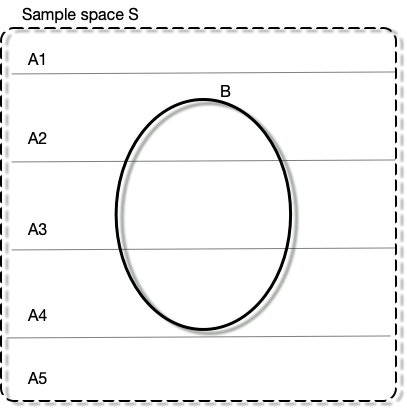
\includegraphics[width=0.8\linewidth]{cc_figure/LOTP} 

}

\caption{Illustration of law of total probability.}\label{fig:lotp}
\end{figure}

For now, this is all the probability theory we need to know!

The next sections expand on the idea of a random variable, the
probability distributions associated with the random variable, what it
means to specify a prior distribution on a parameter, and how the prior
and data can be used to derive the posterior distribution of \(\theta\).

To make the discussion concrete, we will use an example of a discrete
random variable, the Binomial. After discussing this discrete random
variable, we present another example, this time involving a continuous
random variable, the Normal random variable.

The Binomial and Normal cases serve as the canonical examples that we
will need in the initial stages of this book. We will introduce other
random variables as needed: the Uniform, Beta, Poisson, Gamma, and the
Exponential, among others. The properties of all the distributions we
will eventually need are summarized in the appendix.

\section{Discrete random variables: An example using the Binomial
distribution}\label{sec:binomialcloze}

Consider the following sentence:

\emph{``It's raining, I'm going to take the \ldots{}.''}

Suppose that our research goal is to estimate the probability, call it
\(\theta\), of the word ``umbrella'' appearing in this sentence, versus
any other word. If the sentence is completed with the word ``umbrella'',
we will refer to it as a success; any other completion will be referred
to as a failure. This is an example of a Binomial random variable: there
can be only two possible outcomes, a success or a failure, and there is
some true unknown probability \(\theta\) of success that we want to
estimate.\footnote{Technically, each single trial that can result in
  either a success or failure is called a Bernoulli random
  variable---but this random variable is just a special case of the
  Binomial when the number of trials is 1.}

One way to empirically estimate this probability of success is to carry
out a so-called cloze task. In a cloze task, subjects are asked to
complete a fragment of the original sentence, such as ``It's raining,
I'm going to take the \ldots{}''. The predictability or cloze
probability of ``umbrella'' is then calculated as the proportion of
times that the target word ``umbrella'' was produced as an answer by
subjects.

Assume for simplicity that \(10\) subjects are asked to complete the
above sentence; each subject does this task only once. This gives us
independent responses from \(10\) trials that are either coded a success
(``umbrella'' was produced) or as a failure (some other word was
produced). We can sum up the number of sucesses to calculate how many of
the 10 trials had ``umbrella'' as a response. For example, if \(8\)
instances of ``umbrella'' are produced in \(10\) trials, we would
estimate the cloze probability of producing ``umbrella'' would be
\(8/10\).

We can repeatedly generate simulated sequences of the number of
successes in R (later on we will demonstrate how to generate such random
sequences of simulated data). Here is a case where we run the same
experiment \(20\) times (the sample size is \(10\) each time).

\begin{Shaded}
\begin{Highlighting}[]
\KeywordTok{rbinom}\NormalTok{(}\DecValTok{10}\NormalTok{,}\DataTypeTok{n=}\DecValTok{20}\NormalTok{,}\DataTypeTok{prob=}\FloatTok{0.5}\NormalTok{)}
\end{Highlighting}
\end{Shaded}

\begin{verbatim}
##  [1] 7 7 4 7 6 5 6 3 6 6 5 6 7 4 5 7 8 3 5 5
\end{verbatim}

The number of successes in each of the \(20\) simulated experiments
above is being generated by a discrete random variable \(Y\) with a
probability distribution \(p(y|\theta)\) called the \textbf{Binomial
distribution}.

For discrete random variables such as the Binomial, the probability
distribution \(p(y|\theta)\) is called a \textbf{probability mass
function} (PMF). The PMF defines the probability of each possible
outcome. In the above example, with \(n=10\) trials, there are 11
possible outcomes: \(y=0,1,2,...,10\) successes. Which of these outcomes
is most probable depends on the parameter \(\theta\) in the Binomial
distribution that represents the probability of success.

The left-hand side plot in Figure \ref{fig:binomplot} shows an example
of a Binomial PMF with \(10\) trials, with the parameter \(\theta\)
fixed at \(0.5\). Setting \(\theta\) to \(0.5\) leads to a PMF where the
most probable outcome is \(5\) successes out of \(10\). If we had set
\(\theta\) to, say 0.1, then the most probable outcome would be \(1\)
success out of \(10\); and if we had set \(\theta\) to \(0.9\), then the
most probable outcome would be \(9\) successes out of \(10\).

\begin{figure}
\centering
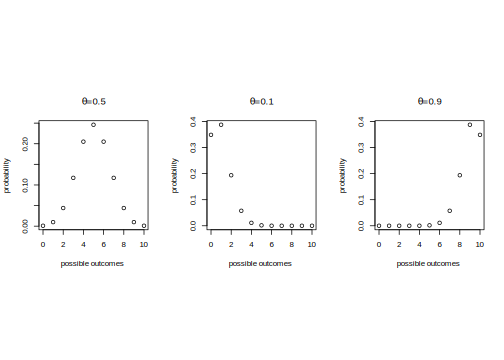
\includegraphics{bookdown_files/figure-latex/binomplot-1.pdf}
\caption{\label{fig:binomplot}Probability mass functions of a binomial
distribution assuming 10 trials, with 50\%, 10\%, and 90\% probability
of success.}
\end{figure}

\begin{rmdnote} to-do bar or line graphs above, instead of
points \end{rmdnote}

The probability mass function for the binomial is written as follows.

\begin{equation}
\hbox{Binomial}(k|n,\theta) = 
\binom{n}{k} \theta^{k} (1-\theta)^{n-k}
\end{equation}

Here, \(n\) represents the total number of trials, \(k\) the number of
successes (this could range from 0 to 10), and \(\theta\) the
probability of success. The term \(\binom{n}{k}\), pronounced
n-choose-k, represents the number of ways in which one can choose \(k\)
successes out of \(n\) trials. For example, 1 success out of 10 can
occur in 10 possible ways: the very first trial could be a 1, the secone
trial could be a 1, etc. The term \(\binom{n}{k}\) expands to
\(\frac{n!}{k!(n-k)!}\). In \texttt{R}, it is computed using the
function \texttt{choose(n,k)}, with \(n\) and \(k\) representing
positive integer values.

When we want to express the fact that the data is assumed to be
generated from a Binomial random variable, we will write
\(Y \sim Binomial(n,\theta)\), where \(\sim\) should be read as ``is
being generated from''. If the data is generated from a random variable
that has some other probability distribution \(f(\theta)\), we will
write \(Y\sim f(\theta)\). Note that we are using \(f(\cdot)\)
synonymously with \(p(\cdot)\) to represent a probability distribution.

\subsection{The mean and variance of the Binomial
distribution}\label{the-mean-and-variance-of-the-binomial-distribution}

It is possible to analytically compute the mean and variance of the PMF
associated with the Binomial random variable \(Y\). Without getting into
the details of how these are derived mathematically, we just state here
that the mean of \(Y\) (also called the expectation, conventionally
written \(E[Y]\)) and variance of \(Y\) (written \(Var(Y)\)) of a
Binomial distribution with parameter \(\theta\) and \(n\) trials are
\(E[Y] = n\theta\) and \(Var(Y) = n\theta (1-\theta)\).

Of course, \(n\) is a fixed number because we decide on the total number
of trials before running the experiment. In the PMF \(\theta\) is also a
fixed value; the only variable in a PMF is \(k\). In real experimental
situations we never know the true value of \(\theta\). But \(\theta\)
can be estimated from the data. From the observed data, we can compute
the estimate of \(\theta\), \(\hat \theta=k/n\). The quantity
\(\hat \theta\) is the observed proportion of successes, and is called
the \textbf{maximum likelihood estimate} of the true (but unknown)
parameter \(\theta\). Once we have estimated \(\theta\) in this way, we
can also obtain an estimate of the variance by computing
\(n\theta (1-\theta)\). These estimates are then used for statistical
inference.

What does the term ``maximum likelihood estimate'' mean? The term
\textbf{likelihood} refers to the Binomial distribution function, i.e.,
the PMF we saw above, \(p(k|n,\theta)\). Recall that the PMF assumes
that \(\theta\) and \(n\) are fixed, and \(k\) will vary from 0 to 10
when the experiment is repeated multiple times. The likelihood function
is the same function as the PMF, \(p(k|n,\theta)\), but assumes that the
data is fixed and only the parameter \(\theta\) varies (from 0 to 1).

For example, suppose you record \(n=10\) trials, and observe \(k=7\)
successes. What is the probability of observing \(7\) successes out of
\(10\)? We need the Binomial distribution to compute this value:

\begin{equation}
\hbox{Binomial}(k=7,n=10|\theta) = 
\binom{10}{7} \theta^{7} (1-\theta)^{10-7}
\end{equation}

Once we have observed the data (k=7 successes), both \(n\) and \(k\) are
fixed. The only variable in the above equation now is \(\theta\): the
above function is now only dependent on the value of \(\theta\).

When the data are fixed, the probability mass function is only dependent
on the value of the parameter \(\theta\), and is called a
\textbf{likelihood function}. It is therefore often expressed as a
function of \(\theta\):

\(p( k=7, n=10 | \theta) = \mathcal{L}(\theta)\)

Since the PMF and the likelihood refer to the same function seen in two
different ways, sometimes the likelihood is written
\(p(\theta | k=7, n=10)\) to distinguish it from the PMF, which has the
data appearing first (\(p(k|n,\theta)\)). We will write both the PMF and
the likelihood identically in this book; context will disambiguate what
we are referring to.

If we now plot the likelihood function for all possible values of
\(\theta\) ranging from \(0\) to \(1\), we get the plot shown in Figure
\ref{fig:binomlik}.

\begin{figure}
\centering
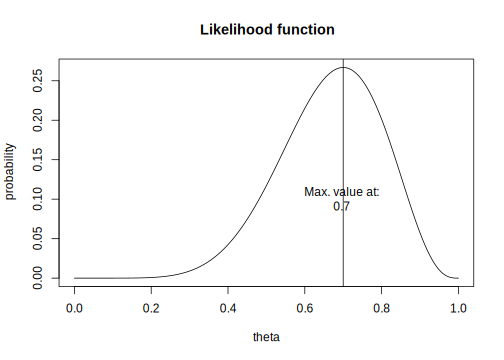
\includegraphics{bookdown_files/figure-latex/binomlik-1.pdf}
\caption{\label{fig:binomlik}The likelihood function for 7 successes out of
10.}
\end{figure}

\begin{rmdnote} DS comment: do we want to show the code for
computing all likelihood values? (maybe this comes later?)
\end{rmdnote}

What is important about this plot is that it shows that, given the data,
the maximum point is at the point \(0.7\), which corresponds to the
estimated mean using the formula shown above: \(k/n = 7/10\). Thus, the
maximum likelihood estimate (MLE) gives us the most likely value that
the parameter \(\theta\) has, given the data. In the binomial, the
proportion of successes \(k/n\) happens to be the maximum likelihood
estimate of the parameter \(\theta\).

It is crucial to note here that the ``most likely'' value of the
parameter is with respect to the data at hand. The data are used to
choose as an estimate of the unknown parameter a value for which the
probability (discrete case) or probability density (continuous case) of
getting the sample values is a maximum. The MLE from a particular sample
of data need not invariably gives us an accurate estimate of \(\theta\).
For example, if we run our experiment for \(10\) trials and get \(1\)
success out of \(10\), the MLE is \(0.10\). We could have just happened
to observe only one success out of ten by chance, even if the true
\(\theta\) were \(0.5\). If you were to repeatedly run the experiment,
in the long run, the MLE computed each time would converge around the
true value of the parameter.

\subsection{What information does a probability distribution
provide?}\label{what-information-does-a-probability-distribution-provide}

In Bayesian data analysis, we will constantly be asking the question:
what information does a probability distribution give us? In particular,
we will treat each parameter \(\theta\) as a random variable; this will
raise questions like: ``what is the probability that the parameter
\(\theta\) lies between two values \(a\) and \(b\)''; and ``what is the
range over which we can be 95\% certain that the true value of the
parameter lies''? In order to be able to answer questions like these, we
need to know what information we can obtain once we have a probability
distribution, and how to extract this information. We therefore discuss
the different kinds of information we can obtain from a probability
distribution. For now we focus only on the Binomial random variable
discussed above.

\subsubsection{Compute the probability of a particular outcome (discrete
case
only)}\label{compute-the-probability-of-a-particular-outcome-discrete-case-only}

The Binomial distribution shown in Figure \ref{fig:binomplot} already
shows the probability of each possible outcome under a different value
for \(\theta\). In R, there is a built-in function that allows us to
calculate the probability of \(k\) successes out of \(n\), given a
particular value of \(k\) (this number constitutes our data), the number
of trials \(n\), and given a particular value of \(\theta\); this is the
\texttt{dbinom} function. For example, the probability of 5 successes
out of 10 when \(\theta\) is 0.5 is:

\begin{Shaded}
\begin{Highlighting}[]
\KeywordTok{dbinom}\NormalTok{(}\DecValTok{5}\NormalTok{,}\DataTypeTok{size=}\DecValTok{10}\NormalTok{,}\DataTypeTok{prob=}\FloatTok{0.5}\NormalTok{)}
\end{Highlighting}
\end{Shaded}

\begin{verbatim}
## [1] 0.246
\end{verbatim}

The probabilities of success when \(\theta\) is 0.1 or 0.9 can be
computed by replacing 0.5 above by each of these probabilities. One can
just do this by giving \texttt{dbinom} a vector of probabilities:

\begin{Shaded}
\begin{Highlighting}[]
\KeywordTok{dbinom}\NormalTok{(}\DecValTok{5}\NormalTok{,}\DataTypeTok{size=}\DecValTok{10}\NormalTok{,}\DataTypeTok{prob=}\KeywordTok{c}\NormalTok{(}\FloatTok{0.1}\NormalTok{,}\FloatTok{0.9}\NormalTok{))}
\end{Highlighting}
\end{Shaded}

\begin{verbatim}
## [1] 0.00149 0.00149
\end{verbatim}

Note that the probability of a particular outcome is only computable in
the discrete case; in the continuous case, this probability will always
be zero (we discuss this when we turn to continuous probability
distributions below).

\subsubsection{Compute the cumulative probability of k or less (more)
than k
successes}\label{compute-the-cumulative-probability-of-k-or-less-more-than-k-successes}

Using the \texttt{dbinom} function, we can compute the cumulative
probability of obtaining 1 or less, 2 or less successes etc. This is
done through a simple summation procedure:

\begin{Shaded}
\begin{Highlighting}[]
\NormalTok{## the cumulative probability of obtaining}
\NormalTok{## 0, 1, or 2 successes out of 10,}
\NormalTok{## with theta=0.5:}
\KeywordTok{dbinom}\NormalTok{(}\DecValTok{0}\NormalTok{,}\DataTypeTok{size=}\DecValTok{10}\NormalTok{,}\DataTypeTok{prob=}\FloatTok{0.5}\NormalTok{)}\OperatorTok{+}\KeywordTok{dbinom}\NormalTok{(}\DecValTok{1}\NormalTok{,}\DataTypeTok{size=}\DecValTok{10}\NormalTok{,}\DataTypeTok{prob=}\FloatTok{0.5}\NormalTok{)}\OperatorTok{+}
\StringTok{  }\KeywordTok{dbinom}\NormalTok{(}\DecValTok{2}\NormalTok{,}\DataTypeTok{size=}\DecValTok{10}\NormalTok{,}\DataTypeTok{prob=}\FloatTok{0.5}\NormalTok{)}
\end{Highlighting}
\end{Shaded}

\begin{verbatim}
## [1] 0.0547
\end{verbatim}

Mathematically, we could write the above summation as:

\begin{equation}
\sum_{k=0}^2 \binom{n}{k} \theta^{k} (1-\theta)^{n-k} 
\end{equation}

An alternative to the cumbersome addition in the R code above is this
more compact statement, which closely mimics the above mathematical
expression:

\begin{Shaded}
\begin{Highlighting}[]
\KeywordTok{sum}\NormalTok{(}\KeywordTok{dbinom}\NormalTok{(}\DecValTok{0}\OperatorTok{:}\DecValTok{2}\NormalTok{,}\DataTypeTok{size=}\DecValTok{10}\NormalTok{,}\DataTypeTok{prob=}\FloatTok{0.5}\NormalTok{))}
\end{Highlighting}
\end{Shaded}

\begin{verbatim}
## [1] 0.0547
\end{verbatim}

R has a built-in function called \texttt{pbinom} that does this
summation for us. If we want to know the probability of \(2\) or less
successes as in the above example, we can write:

\begin{Shaded}
\begin{Highlighting}[]
\KeywordTok{pbinom}\NormalTok{(}\DecValTok{2}\NormalTok{,}\DataTypeTok{size=}\DecValTok{10}\NormalTok{,}\DataTypeTok{prob=}\FloatTok{0.5}\NormalTok{,}\DataTypeTok{lower.tail=}\OtherTok{TRUE}\NormalTok{)}
\end{Highlighting}
\end{Shaded}

\begin{verbatim}
## [1] 0.0547
\end{verbatim}

The specification \texttt{lower.tail=TRUE} ensures that the summation
goes from \(2\) to numbers smaller than \(2\) (which lie in the lower
tail of the distribution in Figure \ref{fig:binomplot}). If we wanted to
know what the probability is of obtaining \(2\) or more successes out of
\(10\), we can set \texttt{lower.tail} to \texttt{FALSE}:

\begin{Shaded}
\begin{Highlighting}[]
\KeywordTok{pbinom}\NormalTok{(}\DecValTok{2}\NormalTok{,}\DataTypeTok{size=}\DecValTok{10}\NormalTok{,}\DataTypeTok{prob=}\FloatTok{0.5}\NormalTok{,}\DataTypeTok{lower.tail=}\OtherTok{FALSE}\NormalTok{)}
\end{Highlighting}
\end{Shaded}

\begin{verbatim}
## [1] 0.945
\end{verbatim}

The cumulative distribution function or CDF can be plotted by computing
the cumulative probabilities for any value \(k\) or less than \(k\),
where \(k\) ranges from \(0\) to \(10\) in our running example. The CDF
is shown in Figure \ref{fig:binomcdf}.

\begin{figure}
\centering
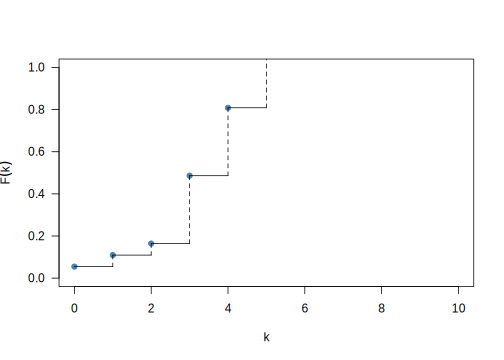
\includegraphics{bookdown_files/figure-latex/binomcdf-1.pdf}
\caption{\label{fig:binomcdf}The cumulative distribution function for a
Binomial distribution assuming 10 trials, with 50\% probability of
success.}
\end{figure}

\subsubsection{Compute the inverse of the cumulative distribution
function (the quantile
function)}\label{compute-the-inverse-of-the-cumulative-distribution-function-the-quantile-function}

We can also find out the value of the variable \(k\) (the quantile) such
that the probability of obtaining \(k\) or less than \(k\) successes is
some specific probability value \(p\). If we switch the x and y axes of
Figure \ref{fig:binomcdf}, we obtain another very useful function, the
inverse CDF.

The inverse of the CDF (known as the quantile function in R because it
returns the quantile, the value k) is available in R as the function
\texttt{qbinom}. The usage is as follows: to find out what the value
\(k\) of the outcome is such that the probability of obtaining \(k\) or
less successes is \(0.37\), type:

\begin{Shaded}
\begin{Highlighting}[]
\KeywordTok{qbinom}\NormalTok{(}\FloatTok{0.37}\NormalTok{,}\DataTypeTok{size=}\DecValTok{10}\NormalTok{,}\DataTypeTok{prob=}\FloatTok{0.5}\NormalTok{)}
\end{Highlighting}
\end{Shaded}

\begin{verbatim}
## [1] 4
\end{verbatim}

\begin{rmdnote} to-do: explain why qbinom(0.77 gives 5 as an
answer and not 4) \end{rmdnote}

\begin{rmdnote} DS comment: maybe it's good to include an
additional Figure for the inverse CDF and an example
\end{rmdnote}

\subsubsection{\texorpdfstring{Generate simulated data from a
\(\hbox{Binomial}(n,\theta)\)
distribution}{Generate simulated data from a \textbackslash{}hbox\{Binomial\}(n,\textbackslash{}theta) distribution}}\label{generate-simulated-data-from-a-hboxbinomialntheta-distribution}

We can generate simulated data from a Binomial distribution by
specifying the number of trials and the probability of success
\(\theta\). In \texttt{R}, we do this as follows:

\begin{Shaded}
\begin{Highlighting}[]
\KeywordTok{rbinom}\NormalTok{(}\DecValTok{1}\NormalTok{,}\DataTypeTok{size=}\DecValTok{10}\NormalTok{,}\DataTypeTok{prob=}\FloatTok{0.5}\NormalTok{)}
\end{Highlighting}
\end{Shaded}

\begin{verbatim}
## [1] 7
\end{verbatim}

\begin{rmdnote} to-do: introduce Bernoulli here and link it
with the code below \end{rmdnote}

The above code generates the number of successes in an experiment with
\(10\) trials. Repeatedly run the above code; you will get different
sequences each time. For each generated sequence, one can calculate the
number of successes by just summing up the vector, or computing its mean
and multiplying by the number of trials, here \(10\):

\begin{Shaded}
\begin{Highlighting}[]
\NormalTok{y<-}\KeywordTok{rbinom}\NormalTok{(}\DecValTok{10}\NormalTok{,}\DataTypeTok{size=}\DecValTok{1}\NormalTok{,}\DataTypeTok{prob=}\FloatTok{0.5}\NormalTok{)}
\KeywordTok{mean}\NormalTok{(y)}\OperatorTok{*}\DecValTok{10}\NormalTok{ ; }\KeywordTok{sum}\NormalTok{(y)}
\end{Highlighting}
\end{Shaded}

\begin{verbatim}
## [1] 6
\end{verbatim}

\begin{verbatim}
## [1] 6
\end{verbatim}

\section{Continuous random variables: An example using the Normal
distribution}\label{continuous-random-variables-an-example-using-the-normal-distribution}

We will now revisit the idea of the random variable using a continuous
distribution. Imagine that you have a vector of reading time data \(y\)
measured in milliseconds and coming from a Normal distribution. The
Normal distribution is defined in terms of two parameters: a mean value
\(\mu\), which determines its center, and the variance \(\sigma^2\),
which determines how much spread there is around this center point.

The probability density function (PDF) of the Normal distribution is
defined as follows:

\begin{equation}
Normal(y|\mu,\sigma)=f(y)= \frac{1}{\sqrt{2\pi \sigma^2}} \exp \left(-\frac{(y-\mu)^2}{2\sigma^2} \right)
\end{equation}

Here, \(\mu\) is some true, unknown mean, and \(\sigma^2\) is some true,
unknown variance of the Normal distribution that the reading times have
been sampled from. There is a built-in function in R that computes the
above function once we specify the mean \(\mu\) and the standard
deviation \(\sigma\) (in R, this parameter is specified in terms of the
standard deviation rather than the variance).

Figure \ref{fig:normdistrn} visualizes the Normal distribution for
particular values of \(\mu\) and \(\sigma\), as a PDF (using
\texttt{dnorm}), a CDF (using \texttt{pnorm}), and the inverse CDF
(using \texttt{qnorm}). It is clear from the figure that these are three
different ways of looking at the same information.

\begin{figure}
\centering
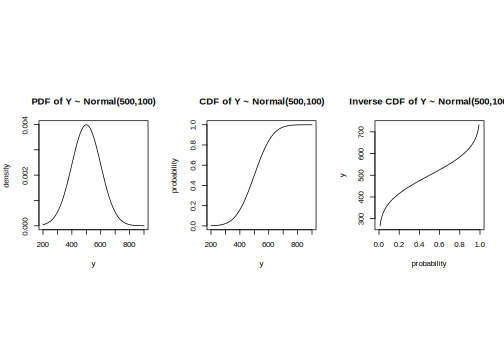
\includegraphics{bookdown_files/figure-latex/normdistrn-1.pdf}
\caption{\label{fig:normdistrn}The PDF, CDF, and inverse CDF for the
\(Normal(\mu=500,\sigma=100)\).}
\end{figure}

\begin{rmdnote} to-do: Maybe this is the place to mention some
interesting properties like: Normal(mu, sigma) = mu + Normal(0,1) *
sigma (We'll use this property a lot later when we code in Stan)
\end{rmdnote}

As in the discrete example, the PDF, CDF, and inverse of the CDF allow
us to ask questions like:

\begin{itemize}
\tightlist
\item
  \textbf{What is the probability of observing values between \(a\) and
  \(b\) from a Normal distribution with mean \(\mu\) and standard
  deviation \(\sigma\)}? Using the above example, we can ask what the
  probability of observing values between 200 and 700 ms:
\end{itemize}

\begin{Shaded}
\begin{Highlighting}[]
\KeywordTok{pnorm}\NormalTok{(}\DecValTok{700}\NormalTok{,}\DataTypeTok{mean=}\DecValTok{500}\NormalTok{,}\DataTypeTok{sd=}\DecValTok{100}\NormalTok{)}\OperatorTok{-}\KeywordTok{pnorm}\NormalTok{(}\DecValTok{200}\NormalTok{,}\DataTypeTok{mean=}\DecValTok{500}\NormalTok{,}\DataTypeTok{sd=}\DecValTok{100}\NormalTok{)}
\end{Highlighting}
\end{Shaded}

\begin{verbatim}
## [1] 0.976
\end{verbatim}

\begin{rmdnote} to-do: add figure illustrating the above
\end{rmdnote}

Notice here that the probability of any point value in a PDF is always
\(0\). This is because the probability in a continuous probability
distribution is the area under the curve, and the area at any point on
the x-axis is always \(0\). The implication here is that we can only ask
about probabilities between two different points; e.g., the probability
that \(Y\) lies between \(a\) and \(b\), or \(P(a<Y<b)\).

\begin{itemize}
\tightlist
\item
  \textbf{What is the quantile \(q\) such that the probability of
  observing that value \(q\) or something less (or more) than it is
  \(p\)}? For example, we can work out the quantile \(q\) such that the
  probability of observing \(q\) or something less than it is 0.975, in
  the Normal(500,100) distribution. Formally, we would write this as
  \(P(Y<a)\).
\end{itemize}

\begin{Shaded}
\begin{Highlighting}[]
\KeywordTok{qnorm}\NormalTok{(}\FloatTok{0.975}\NormalTok{,}\DataTypeTok{mean=}\DecValTok{500}\NormalTok{,}\DataTypeTok{sd=}\DecValTok{100}\NormalTok{)}
\end{Highlighting}
\end{Shaded}

\begin{verbatim}
## [1] 696
\end{verbatim}

The above output says that the probability that the random variable is
less than \(q=695\) is 97.5\%.

\begin{itemize}
\tightlist
\item
  \textbf{Generate simulated data}. Given a vector of \(n\) independent
  and identically distributed data \(y\), i.e., given that each data
  point is being generated independently from
  \(Y \sim Normal(\mu,\sigma)\) for some values of the parameters, the
  maximum likelihood estimates for the expectation and
  variance\footnote{R will compute variance by dividing by \(n-1\), not
    \(n\); this is because dividing by \(n\) gives a biased estimate.
    This is not an important detail for our purposes, and in any case
    for large \(n\) it doesn't really matter whether one divides by
    \(n\) or \(n-1\).} are:
\end{itemize}

\begin{equation}
\bar{y} =  \frac{\sum_{i=1}^n y_i}{n} 
\end{equation}

\begin{equation}
Var(y) = \frac{\sum_{i=1}^n (y_i-
\bar{y})^2}{n}
\end{equation}

For example, we can generate \(10\) data points using the \texttt{rnorm}
function, and then use the simulated data to compute the mean and
variance:

\begin{Shaded}
\begin{Highlighting}[]
\NormalTok{y<-}\KeywordTok{rnorm}\NormalTok{(}\DecValTok{10}\NormalTok{,}\DataTypeTok{mean=}\DecValTok{500}\NormalTok{,}\DataTypeTok{sd=}\DecValTok{100}\NormalTok{)}
\KeywordTok{mean}\NormalTok{(y);}\KeywordTok{var}\NormalTok{(y)}
\end{Highlighting}
\end{Shaded}

\begin{verbatim}
## [1] 560
\end{verbatim}

\begin{verbatim}
## [1] 6778
\end{verbatim}

Again, the sample mean and sample variance computed from a particular
(simulated or real) data-set need not necessarily be close to the true
values of the respective parameters. Especially when sample size is
small, one can end up with misestimates of the mean and sd.

Incidentally, notice that simulated data can be used to generate all
kinds of statistics. For example, we can compute the lower and upper
bounds of a confidence interval from simulated data as follows:

\begin{Shaded}
\begin{Highlighting}[]
\KeywordTok{quantile}\NormalTok{(y,}\DataTypeTok{probs=}\KeywordTok{c}\NormalTok{(}\FloatTok{0.025}\NormalTok{,}\FloatTok{0.975}\NormalTok{))}
\end{Highlighting}
\end{Shaded}

\begin{verbatim}
##  2.5% 97.5% 
##   433   689
\end{verbatim}

Later on, we will be using samples to produce summary statistics like
the ones shown above.

\subsection{An important distinction: probability vs.~density in a
continuous random
variable}\label{an-important-distinction-probability-vs.density-in-a-continuous-random-variable}

In continuous distributions like the Normal discussed above, it is
important to understand that the probability density function or PDF,
\(p(y| \mu, \sigma)\) defines a mapping from the \(y\) values (the
possible values that the data can have) to a quantity called the density
of each possible value. We can see this function in action when we use
\texttt{dnorm} to compute, say, the density value corresponding to
\(y=1\) in the \(Normal(\mu=0,\sigma=1)\) distribution.

\begin{Shaded}
\begin{Highlighting}[]
\NormalTok{## density:}
\KeywordTok{dnorm}\NormalTok{(}\DecValTok{1}\NormalTok{,}\DataTypeTok{mean=}\DecValTok{0}\NormalTok{,}\DataTypeTok{sd=}\DecValTok{1}\NormalTok{)}
\end{Highlighting}
\end{Shaded}

\begin{verbatim}
## [1] 0.242
\end{verbatim}

The quantity above is \emph{not} the probability of observing 1 in this
distribution. As mentioned earlier, probability in a continuous
distribution is the area under the curve, and this area will always be
zero at any point value. If we want to know the probability of obtaining
values between an upper and lower bound \(b\) and \(a\), i.e.,
\(P(a<Y<b)\) where these are two distinct values, we must use the
\texttt{pnorm} function. For example, the probability of observing a
value between +2 and -2 in a Normal distribution with mean 0 and
standard deviation 1 is:

\begin{Shaded}
\begin{Highlighting}[]
\KeywordTok{pnorm}\NormalTok{(}\DecValTok{2}\NormalTok{,}\DataTypeTok{mean=}\DecValTok{0}\NormalTok{,}\DataTypeTok{sd=}\DecValTok{1}\NormalTok{)}\OperatorTok{-}\KeywordTok{pnorm}\NormalTok{(}\OperatorTok{-}\DecValTok{2}\NormalTok{,}\DataTypeTok{mean=}\DecValTok{0}\NormalTok{,}\DataTypeTok{sd=}\DecValTok{1}\NormalTok{)}
\end{Highlighting}
\end{Shaded}

\begin{verbatim}
## [1] 0.954
\end{verbatim}

Notice that the situation is different in discrete random variables.
These have a probability mass function (PMF) associated with them---the
Binomial distribution that we saw earlier is an example. There, the PMF
maps the possible \(y\) values to the probabilities of those values
occurring. That is why, in the Binomial distribution, the probability of
observing exactly 2 successes when sampling from a
\(Binomial(n=10,\theta=0.5)\) can be computed using either
\texttt{dbinom} or \texttt{pbinom}:

\begin{Shaded}
\begin{Highlighting}[]
\KeywordTok{dbinom}\NormalTok{(}\DecValTok{2}\NormalTok{,}\DataTypeTok{size=}\DecValTok{10}\NormalTok{,}\DataTypeTok{prob=}\FloatTok{0.5}\NormalTok{)}
\end{Highlighting}
\end{Shaded}

\begin{verbatim}
## [1] 0.0439
\end{verbatim}

\begin{Shaded}
\begin{Highlighting}[]
\KeywordTok{pbinom}\NormalTok{(}\DecValTok{2}\NormalTok{,}\DataTypeTok{size=}\DecValTok{10}\NormalTok{,}\DataTypeTok{prob=}\FloatTok{0.5}\NormalTok{)}\OperatorTok{-}\KeywordTok{pbinom}\NormalTok{(}\DecValTok{1}\NormalTok{,}\DataTypeTok{size=}\DecValTok{10}\NormalTok{,}\DataTypeTok{prob=}\FloatTok{0.5}\NormalTok{)}
\end{Highlighting}
\end{Shaded}

\begin{verbatim}
## [1] 0.0439
\end{verbatim}

In the second line of code above, we are computing the cumulative
probability of observing two or less successes, minus the probability of
observing one or less successes. This gives us the probability of
observing exactly two successes. The \texttt{dbinom} gives us this same
information.

\section{Bivariate and multivariate
distributions}\label{bivariate-and-multivariate-distributions}

So far, we have only discussed univariate distributions. It is also
possible to specify distributions with two or more dimensions.

\subsection{Example 1: Discrete bivariate
distributions}\label{example-1-discrete-bivariate-distributions}

Starting with the discrete case, consider the discrete bivariate
distribution shown below. These are data from an experiment where, inter
alia, in each trial a Likert acceptability rating and a
question-response accuracy were recorded (the data are from a study by
\citet{AnnaLphd}, used with permission here).

This figure shows the \emph{joint probability mass function} of two
random variables X and Y. The random variable X consists of 7 possible
values (this is the 1-7 Likert response scale), and the random variable
Y is question-response accuracies, with 0 representing incorrect
responses, and 1 representing correct responses.

\begin{Shaded}
\begin{Highlighting}[]
\NormalTok{agrmt<-}\KeywordTok{read.csv}\NormalTok{(}\StringTok{"data/agrmt_discrete_binomial.csv"}\NormalTok{)}
\NormalTok{rating0<-}\KeywordTok{table}\NormalTok{(}\KeywordTok{subset}\NormalTok{(agrmt,accuracy}\OperatorTok{==}\DecValTok{0}\NormalTok{)}\OperatorTok{$}\NormalTok{rating)}
\NormalTok{rating1<-}\KeywordTok{table}\NormalTok{(}\KeywordTok{subset}\NormalTok{(agrmt,accuracy}\OperatorTok{==}\DecValTok{1}\NormalTok{)}\OperatorTok{$}\NormalTok{rating)}

\NormalTok{ratingsbivar<-}\KeywordTok{data.frame}\NormalTok{(}\DataTypeTok{rating0=}\NormalTok{rating0,}\DataTypeTok{rating1=}\NormalTok{rating1)}

\NormalTok{ratingsbivar<-ratingsbivar[,}\KeywordTok{c}\NormalTok{(}\DecValTok{2}\NormalTok{,}\DecValTok{4}\NormalTok{)]}
\KeywordTok{colnames}\NormalTok{(ratingsbivar)<-}\KeywordTok{c}\NormalTok{(}\DecValTok{0}\NormalTok{,}\DecValTok{1}\NormalTok{)}

\NormalTok{## function from the bivariate package:}
\NormalTok{f <-}\StringTok{ }\KeywordTok{cbvpmf}\NormalTok{ (ratingsbivar)}
\KeywordTok{plot}\NormalTok{ (f, }\OtherTok{TRUE}\NormalTok{,}
       \DataTypeTok{arrows=}\OtherTok{FALSE}\NormalTok{)}
\end{Highlighting}
\end{Shaded}

\begin{figure}
\centering
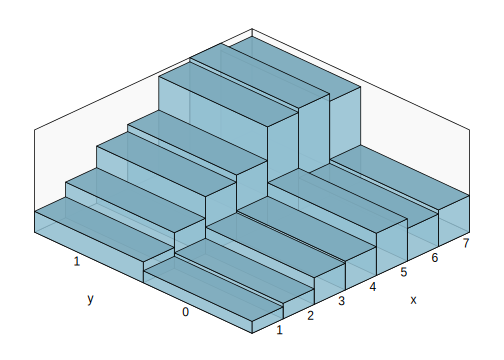
\includegraphics{bookdown_files/figure-latex/bivardiscrete-1.pdf}
\caption{\label{fig:bivardiscrete}Example of a discrete bivariate
distribution. In these data, in every trial, two pieces of information
were collected: Likert responses and yes-no question responses. The
random variable X represents Likert scale responses on a scale of 1-7.
and the random variable Y represents 0, 1 (incorrect, correct) responses
to comprehension questions.}
\end{figure}

One can also display the figure as a table.

\begin{Shaded}
\begin{Highlighting}[]
\NormalTok{probs<-}\KeywordTok{attr}\NormalTok{(f,}\StringTok{"p"}\NormalTok{)}
\KeywordTok{t}\NormalTok{(probs)}
\end{Highlighting}
\end{Shaded}

\begin{verbatim}
##     [,1]   [,2]   [,3]   [,4]   [,5]   [,6]   [,7]
## 0 0.0179 0.0233 0.0400 0.0431 0.0633 0.0489 0.0549
## 1 0.0312 0.0533 0.0857 0.0964 0.1469 0.1532 0.1420
\end{verbatim}

For each possible value of X and Y, we have a joint probability. Given
such a bivariate distribution, there are two useful quantities we can
compute: the \emph{marginal} distributions (\(p_{X}\) and \(p_Y\)), and
the \emph{conditional} distributions (\(p_{X|Y}\) and \(p_{Y|X}\)).\\
The table below shows the joint probability mass function
\(p_{X,Y}(x,y)\).

\begin{table}[!htbp] 
\begin{center}
\begin{tabular}{c|ccccccc}
$p_{X,Y}$ & x=1 & x=2 & x=3 & x=4 & x=5 & x=6 & x=7\\
\hline
y = 0 & 0.018 & 0.023 & 0.040 & 0.043 & 0.063 & 0.049 & 0.055\\
y = 1 & 0.031 & 0.053 & 0.086 & 0.096 &  0.147 & 0.153 &  0.142\\
\end{tabular}
\end{center}
\caption{The joint PMF for two random variables $X$ and $Y$.}\label{discretebivartable}
\end{table}

The marginal distribution \(p_Y\) is defined as follows. \(S_{X}\) is
the support of X, i.e., all the possible values of X.

\begin{equation}
p_{Y}(y)=\sum_{x\in S_{X}}p_{X,Y}(x,y).\label{eq-marginal-pmf}
\end{equation}

Similarly, the marginal distribution \(p_X\) is defined as:

\begin{equation}
p_{X}(x)=\sum_{y\in S_{Y}}p_{X,Y}(x,y).\label{eq-marginal-pmf2}
\end{equation}

\(p_Y\) is easily computed, by summing up the rows; and \(p_X\) by
summing up the columns. You can see why this is called the marginal
distribution; the result appears in the margins of the table.

\begin{Shaded}
\begin{Highlighting}[]
\CommentTok{#P(Y)}
\NormalTok{(PY<-}\KeywordTok{rowSums}\NormalTok{(}\KeywordTok{t}\NormalTok{(probs)))}
\end{Highlighting}
\end{Shaded}

\begin{verbatim}
##     0     1 
## 0.291 0.709
\end{verbatim}

\begin{Shaded}
\begin{Highlighting}[]
\KeywordTok{sum}\NormalTok{(PY) ## sums to 1}
\end{Highlighting}
\end{Shaded}

\begin{verbatim}
## [1] 1
\end{verbatim}

\begin{Shaded}
\begin{Highlighting}[]
\CommentTok{#P(X)}
\NormalTok{(PX<-}\KeywordTok{colSums}\NormalTok{(}\KeywordTok{t}\NormalTok{(probs)))}
\end{Highlighting}
\end{Shaded}

\begin{verbatim}
## [1] 0.0491 0.0766 0.1257 0.1394 0.2102 0.2020 0.1969
\end{verbatim}

\begin{Shaded}
\begin{Highlighting}[]
\KeywordTok{sum}\NormalTok{(PX) ## sums to 1}
\end{Highlighting}
\end{Shaded}

\begin{verbatim}
## [1] 1
\end{verbatim}

The marginal probabilities sum to 1, as they should. The table below
shows the marginal probabilities.

\small

\begin{table}[!htbp]
\begin{center}
\begin{tabular}{c|ccccccc|c}
$p_{X,Y}$ & x=1 & x=2 & x=3 & x=4 & x=5 & x=6 & x=7 & P(Y)\\
\hline
y = 0 & 0.018 & 0.023 & 0.040 & 0.043 & 0.063 & 0.049 & 0.055 &  \textbf{0.291}\\
y = 1 & 0.031 & 0.053 & 0.086 & 0.096 &  0.147 & 0.153 &  0.142 &  \textbf{0.709}\\
\hline
P(X) & \textbf{0.049} & \textbf{0.077} & \textbf{0.126} & \textbf{0.139} & \textbf{0.210} & \textbf{0.202} & \textbf{0.197}\\
\end{tabular}
\end{center}
\caption{The joint and marginal distributions of X and Y.}\label{discretebivartable2}
\end{table}

\normalsize

Notice that to compute the marginal distribution of X, one is summing
over all the Ys; and to compute the marginal distribution of Y, one sums
over all the X's. We say that we are \emph{marginalizing out} the random
variable that we are summing over. One can visualize the two marginal
distributions using barplots.

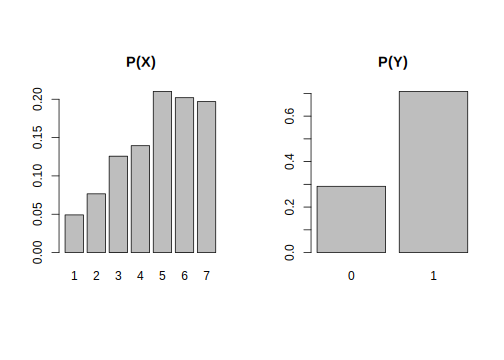
\includegraphics{bookdown_files/figure-latex/unnamed-chunk-24-1.pdf}

For computing conditional distributions, recall that conditional
probability is defined as:

\begin{equation}
p_{X\mid Y}(x\mid y) = \frac{p_{X,Y}(x,y)}{p_Y(y)}  
\end{equation}

and

\begin{equation}
p_{Y\mid X}(x\mid y) = \frac{p_{X,Y}(x,y)}{p_X(x)}  
\end{equation}

The conditional distribution of a random variable \(X\) given that
\(Y=y\), where \(y\) is some specific (fixed) value, is:

\begin{equation}
p_{X\mid Y} (x\mid y) = \frac{p_{X,Y}(x,y)}{p_Y(y)} \quad \hbox{provided } p_Y(y)=P(Y=y)>0
\end{equation}

As an example, let's consider how \(p_{X\mid Y}\) would be computed. The
possible values of \(y\) are \(0,1\), and so we have to find the
conditional distribution (defined above) for each of these values. I.e.,
we have to find \(p_{X\mid Y}(x\mid y=0)\), and
\(p_{X\mid Y}(x\mid y=1)\).

Let's do the calculation for \(p_{X\mid Y}(x\mid y=0)\).

\begin{equation}
\begin{split}
p_{X\mid Y} (1\mid 0) =& \frac{p_{X,Y}(1,0)}{p_Y(0)}\\
    =&  \frac{0.018}{0.291}\\
    =& 0.062
\end{split} 
\end{equation}

This conditional probability value will occupy the cell X=1, Y=0 in the
table below summarizing the conditional probability distribution
\(p_{X|Y}\). In this way, one can fill in the entire table, which will
then represent the conditional distributions \(p_{X|Y=0}\) and
\(p_{X|Y=1}\). The reader may want to take a few minutes to complete the
table.

\begin{table}[!htbp]
\begin{center}
\begin{tabular}{c|ccccccc}
    & x=1 & x=2 & x=3 & x=4 & x=5 & x=6 & x=7\\ 
\hline  
$p_{X\mid Y}(x\mid y=0)$  & 0.062 &  & & & & & \\
$p_{X\mid Y}(x\mid y=1)$  &  &  & & & & &  \\
\end{tabular}
\end{center}
\caption{The conditional probability distribution of X given Y.}
\label{XgivenY}
\end{table}

Similarly, one can construct a table that shows \(p_{Y|X}\).

\subsection{Example 2: Continuous bivariate
distributions}\label{example-2-continuous-bivariate-distributions}

Consider now the continuous bivariate case; this time, we will use
simulated data. Consider two normal random variables \(X\) and \(Y\),
each of which coming from, for example, a Normal(0,1) distribution, with
some correlation \(\rho\) between the two random variables.

A bivariate distribution for two random variables \(X\) and \(Y\), each
of which comes from a normal distribution, is expressed in terms of the
means and standard deviations of each of the two distributions, and the
correlation \(\rho\) between them. The standard deviations and
correlation are expressed in a special form of a \(2\times 2\) matrix
called a variance-covariance matrix \(\Sigma\). If \(\rho_u\) is the
correlation between the two random variables, and \(\sigma _{x}\) and
\(\sigma _{y}\) the respective standard deviations, the
variance-covariance matrix is written as:

\begin{equation}\label{eq:covmatfoundations}
\Sigma
=
\begin{pmatrix}
\sigma _{x}^2  & \rho\sigma _{x}\sigma _{y}\\
\rho\sigma _{x}\sigma _{y}    & \sigma _{y}^2\\
\end{pmatrix}
\end{equation}

The off-diagonals of this matrix contain the covariance between \(X\)
and \(Y\).

The joint distribution of \(X\) and \(Y\) is defined as follows:

\begin{equation}\label{eq:jointpriordistfoundations}
\begin{pmatrix}
  X \\ 
  Y \\
\end{pmatrix}
\sim 
\mathcal{N}_2 \left(
\begin{pmatrix}
  0 \\
  0 \\
\end{pmatrix},
\Sigma
\right)
\end{equation}

The joint PDF is written with reference to the two variables
\(f_{X,Y}(x,y)\). It has the property that the area under the curve sums
to 1. Formally, we would write this as a double integral: we are summing
up the area under the curve for both dimensions X and Y (hence two
integrals).

\begin{equation}
\iint_{S_{X,Y}} f_{X,Y}(x,y)\, dx dy = 1
\end{equation}

Here, the terms \(dx\) and \(dy\) express the fact that we are summing
the area under the curve along the X axis and the Y axis.

The joint CDF would be written as follows. The equation below gives us
the probability of observing a value like \((u,v)\) or some value
smaller than that (i.e., some \((u',v')\), such that \(u'<u\) and
\(v'<v\).

\begin{equation}
\begin{split}
F_{X,Y}(u,v) =& P(X<u,Y<v)\\
             =& \int_{-\infty}^u \int_{-\infty}^v f_{X,Y}(x,y)\, dy dx \hbox{ for } (x,y)\in \mathbb{R}^2\\
\end{split}
\end{equation}

As an aside, notice that the support for the normal distribution ranges
from minus infinity to plus infinity. There can however be other PDFs
with a more limited support; an example would be a normal distribution
whose pdf \(f(x)\) is such that the lower bound is truncated at, say, 0.
In such a case, the area under the range \(\int_{-\infty}^0 f(x) \, dx\)
will be 0 because the range lies outside the support of the truncated
normal distribution.

Just as in the discrete case, the marginal distributions can be derived
by marginalizing out the other random variable:

\begin{equation}
f_X(x) = \int_{S_Y} f_{X,Y}(x,y)\, dy \quad f_Y(y) = \int_{S_X} f_{X,Y}(x,y)\, dx
\end{equation}

Here, \(S_X\) and \(S_Y\) are the respective supports.

Here, the integral sign \(\int\) is the continuous equivalent of the
summation sign \(\sum\) in the discrete case. Luckily, we will never
have to compute such integrals ourselves; but it is important to
appreciate how a marginal distribution arises from a bivariate
distributation---by integrating out or marginalizing out the other
random variable.

A visualization will help. The figures below shows a bivariate
distribution with correlation zero (Figure \ref{fig:zerocor}), a
positive (Figure \ref{fig:poscor}) and a negative correlation (Figure
\ref{fig:negcor}).

\begin{figure}
\centering
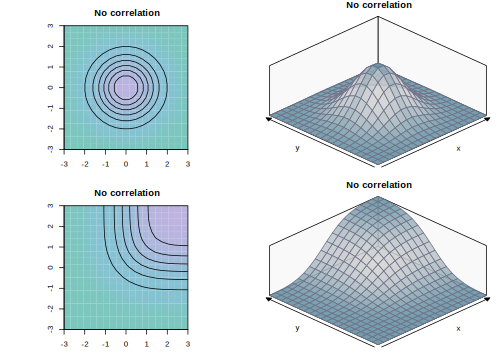
\includegraphics{bookdown_files/figure-latex/zerocor-1.pdf}
\caption{\label{fig:zerocor}A bivariate Normal distribution with zero
correlation. Shown are four plots: the top-right plot shows the
three-dimensional bivariate density, the top-left plot the contour plot
of the distribution (seen from above). The lower plots show the
cumulative distribution function from two views, as a three-dimensional
plot and as a contour plot.}
\end{figure}

\begin{figure}
\centering
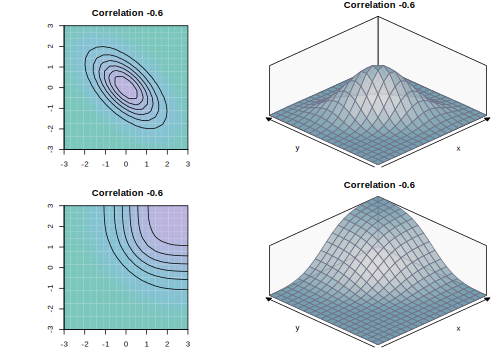
\includegraphics{bookdown_files/figure-latex/poscor-1.pdf}
\caption{\label{fig:poscor}A bivariate Normal distribution with a positive
correlation of -0.6. Shown are four plots: the top-right plot shows the
three-dimensional bivariate density, the top-left plot the contour plot
of the distribution (seen from above). The lower plots show the
cumulative distribution function from two views, as a three-dimensional
plot and as a contour plot.}
\end{figure}

\begin{figure}
\centering
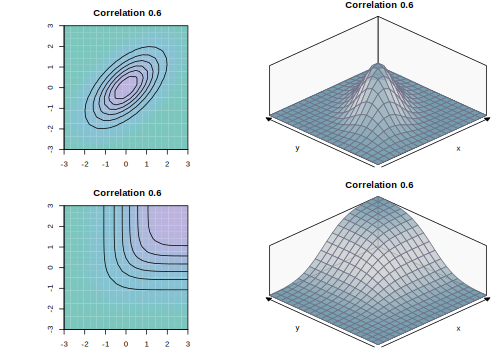
\includegraphics{bookdown_files/figure-latex/negcor-1.pdf}
\caption{\label{fig:negcor}A bivariate Normal distribution with a negative
correlation of -0.6. Shown are four plots: the top-right plot shows the
three-dimensional bivariate density, the top-left plot the contour plot
of the distribution (seen from above). The lower plots show the
cumulative distribution function from two views, as a three-dimensional
plot and as a contour plot.}
\end{figure}

In this book, we will make use of such multivariate distributions a lot,
and it will soon become important to know how to generate simulated
bivariate or multivariate data that is correlated. So let's look at that
next.

\subsection{Generate simulated bivariate (multivariate)
data}\label{generate-simulated-bivariate-multivariate-data}

Suppose we want to generate 100 correlated pairs of data, with
correlation \(\rho=0.6\). The two random variables have mean 0, and
standard deviations 5 and 10 respectively.

Here is how we would generate such data. First, define a
variance-covariance matrix; then, use the multivariate analog of the
\texttt{rnorm} function, \texttt{mvrnorm}, to generate \(100\)
data-points.

\begin{Shaded}
\begin{Highlighting}[]
\KeywordTok{library}\NormalTok{(MASS)}
\NormalTok{## define a variance-covariance matrix:}
\NormalTok{Sigma<-}\KeywordTok{matrix}\NormalTok{(}\KeywordTok{c}\NormalTok{(}\DecValTok{5}\OperatorTok{^}\DecValTok{2}\NormalTok{,}\DecValTok{5}\OperatorTok{*}\DecValTok{10}\OperatorTok{*}\NormalTok{.}\DecValTok{6}\NormalTok{,}\DecValTok{5}\OperatorTok{*}\DecValTok{10}\OperatorTok{*}\NormalTok{.}\DecValTok{6}\NormalTok{,}\DecValTok{10}\OperatorTok{^}\DecValTok{2}\NormalTok{),}
              \DataTypeTok{byrow=}\OtherTok{FALSE}\NormalTok{,}\DataTypeTok{ncol=}\DecValTok{2}\NormalTok{)}
\NormalTok{## generate data:}
\NormalTok{u<-}\KeywordTok{mvrnorm}\NormalTok{(}\DataTypeTok{n=}\DecValTok{100}\NormalTok{,}
           \DataTypeTok{mu=}\KeywordTok{c}\NormalTok{(}\DecValTok{0}\NormalTok{,}\DecValTok{0}\NormalTok{),}
           \DataTypeTok{Sigma=}\NormalTok{Sigma)}
\KeywordTok{head}\NormalTok{(u)}
\end{Highlighting}
\end{Shaded}

\begin{verbatim}
##        [,1]  [,2]
## [1,]  1.801 -5.02
## [2,]  2.466  7.92
## [3,] -0.672  7.71
## [4,] -3.662 -9.29
## [5,] -0.961  0.74
## [6,] 11.522 19.53
\end{verbatim}

A plot confirms that the simulated data are positively correlated.

\begin{Shaded}
\begin{Highlighting}[]
\KeywordTok{plot}\NormalTok{(u[,}\DecValTok{1}\NormalTok{],u[,}\DecValTok{2}\NormalTok{])}
\end{Highlighting}
\end{Shaded}

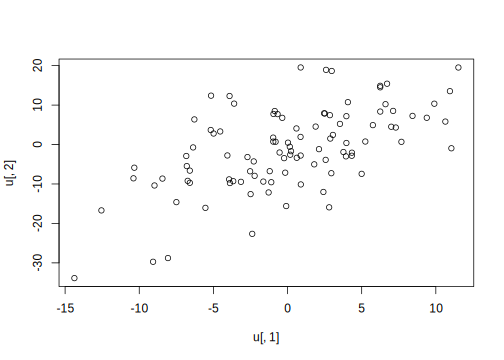
\includegraphics{bookdown_files/figure-latex/unnamed-chunk-26-1.pdf}

As an exercise, try changing the correlation to \(0\) or to \(-0.6\),
and then plot the bivariate distribution that results.

One final useful thing to notice about the variance-covariance matrix is
that it can be decomposed into the component standard deviations and an
underlying correlation matrix. For example, consider the matrix above:

\begin{Shaded}
\begin{Highlighting}[]
\NormalTok{Sigma}
\end{Highlighting}
\end{Shaded}

\begin{verbatim}
##      [,1] [,2]
## [1,]   25   30
## [2,]   30  100
\end{verbatim}

One can decompose the matrix as follows. The matrix can be seen as the
product of a diagonal matrix of the standard deviations and the
correlation matrix:

\begin{Shaded}
\begin{Highlighting}[]
\NormalTok{## sds:}
\NormalTok{(sds<-}\KeywordTok{c}\NormalTok{(}\DecValTok{5}\NormalTok{,}\DecValTok{10}\NormalTok{))}
\end{Highlighting}
\end{Shaded}

\begin{verbatim}
## [1]  5 10
\end{verbatim}

\begin{Shaded}
\begin{Highlighting}[]
\NormalTok{## diagonal matrix:}
\NormalTok{(sd_diag<-}\KeywordTok{diag}\NormalTok{(sds))}
\end{Highlighting}
\end{Shaded}

\begin{verbatim}
##      [,1] [,2]
## [1,]    5    0
## [2,]    0   10
\end{verbatim}

\begin{Shaded}
\begin{Highlighting}[]
\NormalTok{## correlation matrix:}
\NormalTok{(corrmatrix<-}\KeywordTok{matrix}\NormalTok{(}\KeywordTok{c}\NormalTok{(}\DecValTok{1}\NormalTok{,}\FloatTok{0.6}\NormalTok{,}\FloatTok{0.6}\NormalTok{,}\DecValTok{1}\NormalTok{),}\DataTypeTok{ncol=}\DecValTok{2}\NormalTok{))}
\end{Highlighting}
\end{Shaded}

\begin{verbatim}
##      [,1] [,2]
## [1,]  1.0  0.6
## [2,]  0.6  1.0
\end{verbatim}

Given these two matrices, one can reassemble the variance-covariance
matrix:

\begin{Shaded}
\begin{Highlighting}[]
\NormalTok{sd_diag}\OperatorTok\NormalTok{corrmatrix}\OperatorTok\NormalTok{sd_diag                   }
\end{Highlighting}
\end{Shaded}

\begin{verbatim}
##      [,1] [,2]
## [1,]   25   30
## [2,]   30  100
\end{verbatim}

There is a built-in convenience function, \texttt{sdcor3cov} in the
\texttt{SIN} package that does this calculation, taking the vector of
standard deviatios (not the diagonal matrix) and the correlation matrix
to yield the variance-covariance matrix:

\begin{Shaded}
\begin{Highlighting}[]
\NormalTok{SIN}\OperatorTok{::}\KeywordTok{sdcor2cov}\NormalTok{(}\DataTypeTok{stddev=}\NormalTok{sds,}\DataTypeTok{corr=}\NormalTok{corrmatrix)}
\end{Highlighting}
\end{Shaded}

\begin{verbatim}
##      [,1] [,2]
## [1,]   25   30
## [2,]   30  100
\end{verbatim}

We will be using this function a lot when simulating data from
hierarchical models.

\section{An important concept: The marginal likelihood (integrating out
a parameter)}\label{sec:marginal}

Here, we introduce a concept that will turn up many times in this book.
The concept we unpack here is called ``integrating out a parameter''. We
will need this when we encounter Bayes' rule in the next chapter, and
when we use Bayes factors later in the book.

Integrating out a parameter refers to the following situation. Suppose
we have a Binomial random variable \(Y\) with PMF \(p(Y)\). Suppose also
that this PMF is defined in terms of parameter \(\theta\) that can have
only three possible values, \(0.1, 0.5, 0.9\), each with equal
probability. In other words, the probability that \(\theta\) is
\(0.1, 0.5,\) or \(0.9\) is 1/3 each.

We stick with our earlier example of \(n=10\) trials and \(k=8\)
successes. The \textbf{likelihood function} then is

\begin{equation}
p(k=8,n=10|\theta) = \binom{10}{8} \theta^8 (1-\theta)^{2}
\end{equation}

There is a related concept of \textbf{marginal likelihood}, which we can
write here as \(p(k=8,n=10)\). Marginal likelihood is the likelihood
computed by ``marginalizing'' out the parameter \(\theta\): for each
possible value that the parameter \(\theta\) can have, we compute the
likelihood at that value and multiply that likelihood with the
probability/density of that \(\theta\) value occurring. Then we sum up
each of the products computed in this way. Mathematically, this means
that we carry out the following operation.

In our example, there are three possible values of \(\theta\), call them
\(\theta_1=0.1\), \(\theta_2=0.5\), and \(\theta_3=0.9\). Each has
probability \(1/3\); so \(p(\theta_1)=p(\theta_2)=p(\theta_3)=1/3\).
Given this information, we can compute the marginal likelihood as
follows:

\begin{equation}
\begin{split}
p(k=8,n=10) =& \binom{10}{8} \theta_1^8 (1-\theta_1)^{2} \times p(\theta_1) \\
            +& \binom{10}{8} \theta_2^8 (1-\theta_2)^{2}\times p(\theta_2) \\
            +& \binom{10}{8} \theta_3^8 (1-\theta_3)^{2}\times p(\theta_3)
\end{split}
\end{equation}

Writing the \(\theta\) values and their probabilities, we get:

\begin{equation}
\begin{split}
p(k=8,n=10) =& \binom{10}{8} 0.1^8 (1-0.1)^{2} \times \frac{1}{3} \\
            +& \binom{10}{8} 0.5^8 (1-0.5)^{2}\times \frac{1}{3} \\
            +& \binom{10}{8} 0.9^8 (1-0.9)^{2}\times \frac{1}{3}
\end{split}
\end{equation}

We can simplify this summation by collecting together the common terms:

\begin{equation}
\begin{split}
p(k=8,n=10) =& \frac{1}{3} [\binom{10}{8}  0.1^8 (1-0.1)^{2} \\
+& \binom{10}{8} 0.5^8 (1-0.5)^{2} \\
+& \binom{10}{8} 0.9^8 (1-0.9)^{2}] \\
=& 0.058 
\end{split}
\end{equation}

Thus, a marginal likelihood is a kind of weighted sum of the likelihood,
weighted by the possible values of the parameter.\footnote{Where does
  the above formula come from? It falls out from the law of total
  probability discussed above!}

The above example was contrived, because we stated that the parameter
\(\theta\) has only three possible values. In reality, because the
parameter \(\theta\) can have all possible values between 0 and 1, the
summation has to be done over a continuous space \([0,1]\). The way this
summation is expressed in mathematics is through the integral symbol:

\begin{equation}
p(k=8,n=10) = \int_0^1 \binom{10}{8} \theta^8 (1-\theta)^{2}\, d\theta
\end{equation}

This statement is saying exactly what we computed above, except that the
summation is being done over a continuous space ranging from 0 to 1. We
say that the parameter \(\theta\) has been integrated out, or
marginalized. Integrating out a parameter will be a very common
operation in this book, but fortunately we will never have to do the
calculation ourselves. For the above case, we can easily compute the
integral in R:

\begin{Shaded}
\begin{Highlighting}[]
\NormalTok{BinLik<-}\ControlFlowTok{function}\NormalTok{(theta)\{}
  \KeywordTok{choose}\NormalTok{(}\DecValTok{10}\NormalTok{,}\DecValTok{8}\NormalTok{)}\OperatorTok{*}\NormalTok{theta}\OperatorTok{^}\DecValTok{8} \OperatorTok{*}\StringTok{ }\NormalTok{(}\DecValTok{1}\OperatorTok{-}\NormalTok{theta)}\OperatorTok{^}\DecValTok{2}
\NormalTok{\}}
\KeywordTok{integrate}\NormalTok{(BinLik,}\DataTypeTok{lower=}\DecValTok{0}\NormalTok{,}\DataTypeTok{upper=}\DecValTok{1}\NormalTok{)}\OperatorTok{$}\NormalTok{value}
\end{Highlighting}
\end{Shaded}

\begin{verbatim}
## [1] 0.0909
\end{verbatim}

This completes our discussion of random variables and probability
distributions. We now summarize what we have learnt so far.

\section{Summary of useful R functions relating to
distributions}\label{summary-of-useful-r-functions-relating-to-distributions}

Table \ref{tab:dpqrfunctions} summarizes the different functions
relating to PMFs and PDFs, using the Binomial and Normal as examples.

\begin{longtable}[]{@{}lcc@{}}
\caption{\label{tab:dpqrfunctions} Important R functions relating to random
variables.}\tabularnewline
\toprule
& Discrete & Continuous\tabularnewline
\midrule
\endfirsthead
\toprule
& Discrete & Continuous\tabularnewline
\midrule
\endhead
Example: & Binomial(\(y|n,\theta\)) &
Normal(\(y|\mu,\sigma\))\tabularnewline
Likelihood function & dbinom & dnorm\tabularnewline
Prob Y=y & dbinom & always 0\tabularnewline
Prob \(Y\geq y, Y\leq y, y_1<Y<y_2\) & pbinom & pnorm\tabularnewline
Inverse CDF & qbinom & qnorm\tabularnewline
Generate simulated data & rbinom & rnorm\tabularnewline
\bottomrule
\end{longtable}

Later on, we will use other distributions, such as the Uniform, Beta,
etc., and each of these has their own set of d-p-q-r functions in R. The
appendix summarizes the properties of the distributions that we will
need in this book.

\section{Summary of concepts introduced in this
chapter}\label{summary-of-concepts-introduced-in-this-chapter}
\begin{rmdnote} to-do: add summary \end{rmdnote}
\section{Further reading}\label{further-reading}

A quick review of the mathematical foundations needed for statistics is
available in the short book by \citet{fox2009mathematical}.
\citet{morin2016probability} and \citet{blitzstein2014introduction} are
accessible introductions to probability theory.

\section{Exercises}\label{exercises}

\subsection{\texorpdfstring{Practice using the \texttt{pnorm}
function}{Practice using the pnorm function}}\label{practice-using-the-pnorm-function}

\subsubsection{Part 1}\label{part-1}

Given a normal distribution with mean \texttt{74} and standard deviation
\texttt{101}, use the pnorm function to calculate the probability of
obtaining values between \texttt{100} and \texttt{45} from this
distribution.

\subsubsection{Part 2}\label{part-2}

Calculate the following probabilities. Given a normal distribution with
mean \texttt{53} and standard deviation \texttt{2}, what is the
probability of getting

\begin{itemize}
\tightlist
\item
  a score of \texttt{48} or less
\item
  a score of \texttt{48} or more
\item
  a score of \texttt{52} or more
\end{itemize}

\subsubsection{Part 3}\label{part-3}

Given a normal distribution with mean \texttt{46} and standard deviation
\texttt{7}, what is the probability of getting

\begin{itemize}
\tightlist
\item
  a score of \texttt{41} or less.
\item
  a score between \texttt{43} and \texttt{49}.
\item
  a score of \texttt{47} or more.
\end{itemize}

\subsection{\texorpdfstring{Practice using the \texttt{qnorm}
function}{Practice using the qnorm function}}\label{practice-using-the-qnorm-function}

\subsubsection{Part 1}\label{part-1-1}

Consider a normal distribution with mean 1 and standard deviation 1.

Compute the lower and upper boundaries such that:

\begin{itemize}
\tightlist
\item
  the area (the probability) to the left of the lower boundary is
  \texttt{0.32}.
\item
  the area (the probability) to the left of the upper boundary is
  \texttt{0.63}.
\end{itemize}

\subsubsection{Part 2}\label{part-2-1}

Given a normal distribution with mean \texttt{53.938} and standard
deviation \texttt{1.362}. There exist two quantiles, the lower quantile
q1 and the upper quantile q2, that are equidistant from the mean
\texttt{53.938}, such that the area under the curve of the Normal
between q1 and q2 is \texttt{80}\%. Find q1 and q2.

\subsection{\texorpdfstring{Practice using
\texttt{qt}}{Practice using qt}}\label{practice-using-qt}

Take an independent random sample of size \texttt{140} from a normal
distribution with mean \texttt{175}, and standard deviation \texttt{78}.
Next, we are going to pretend we don't know the population parameters
(the mean and standard deviation). We compute the MLEs of the mean and
standard deviation using the data and get the sample mean
\texttt{173.423} and the sample standard deviation \texttt{73.971}.

\begin{itemize}
\tightlist
\item
  Compute the estimated standard error using the sample standard
  deviation provided above.
\item
  What are your degrees of freedom for the relevant t-distribution?
\item
  Calculate the \textbf{absolute} critical t-value for a 95\% confidence
  interval using the relevant degrees of freedom you just wrote above.
\item
  Next, compute the lower bound of the 95\% confidence interval using
  the estimated standard error and the critical t-value.
\item
  Finally, compute the upper bound of the 95\% confidence interval using
  the estimated standard error and the critical t-value.
\end{itemize}

\subsection{Maximum likelihood estimation
1}\label{maximum-likelihood-estimation-1}

Given the data point \texttt{6.453}. The function \texttt{dnorm} gives
the likelihood given a data point (or multiple data points) and a value
for the mean and the standard deviation (sd). Using \texttt{dnorm},
compute

\begin{itemize}
\tightlist
\item
  the likelihood of the data point \texttt{6.453} assuming a mean of
  \texttt{12} and standard deviation 5.
\item
  the likelihood of the data point \texttt{6.453} assuming a mean of
  \texttt{11} and standard deviation 5.
\item
  the likelihood of the data point \texttt{6.453} assuming a mean of
  \texttt{10} and standard deviation 5.
\item
  the likelihood of the data point \texttt{6.453} assuming a mean of
  \texttt{9} and standard deviation 5.
\end{itemize}

\subsection{Maximum likelihood estimation
2}\label{maximum-likelihood-estimation-2}

You are given \(10\) independent and identically distributed data points
that are assumed to come from a Normal distribution with unknown mean
and unknown standard deviation:

\begin{Shaded}
\begin{Highlighting}[]
\NormalTok{x}
\end{Highlighting}
\end{Shaded}

\begin{verbatim}
##  [1] 501 518 524 489 505 514 498 498 497 506
\end{verbatim}

The function \texttt{dnorm} gives the likelihood given multiple data
points and a value for the mean and the standard deviation. The
log-likelihood can be computed by typing \texttt{dnorm(...,log=TRUE)}.

The product of the likelihoods for two independent data points can be
computed like this: Suppose we have two independent and identically
distributed data points 5 and 10. Then, assuming that the Normal
distribution they come from has mean 10 and standard deviation 2, the
joint likelihood of these is:

\begin{Shaded}
\begin{Highlighting}[]
\KeywordTok{dnorm}\NormalTok{(}\DecValTok{5}\NormalTok{,}\DataTypeTok{mean=}\DecValTok{10}\NormalTok{,}\DataTypeTok{sd=}\DecValTok{2}\NormalTok{)}\OperatorTok{*}\KeywordTok{dnorm}\NormalTok{(}\DecValTok{10}\NormalTok{,}\DataTypeTok{mean=}\DecValTok{10}\NormalTok{,}\DataTypeTok{sd=}\DecValTok{2}\NormalTok{)}
\end{Highlighting}
\end{Shaded}

\begin{verbatim}
## [1] 0.00175
\end{verbatim}

It is easier to do this on the log scale, because then one can add
instead of multiplying. This is because
\(\log(x\times y)= \log(x) + \log(y)\). For example:

\begin{Shaded}
\begin{Highlighting}[]
\KeywordTok{log}\NormalTok{(}\DecValTok{2}\OperatorTok{*}\DecValTok{3}\NormalTok{)}
\end{Highlighting}
\end{Shaded}

\begin{verbatim}
## [1] 1.79
\end{verbatim}

\begin{Shaded}
\begin{Highlighting}[]
\KeywordTok{log}\NormalTok{(}\DecValTok{2}\NormalTok{) }\OperatorTok{+}\StringTok{ }\KeywordTok{log}\NormalTok{(}\DecValTok{3}\NormalTok{)}
\end{Highlighting}
\end{Shaded}

\begin{verbatim}
## [1] 1.79
\end{verbatim}

So the joint log likelihood of the two data points is:

\begin{Shaded}
\begin{Highlighting}[]
\KeywordTok{dnorm}\NormalTok{(}\DecValTok{5}\NormalTok{,}\DataTypeTok{mean=}\DecValTok{10}\NormalTok{,}\DataTypeTok{sd=}\DecValTok{2}\NormalTok{,}\DataTypeTok{log=}\OtherTok{TRUE}\NormalTok{)}\OperatorTok{+}\KeywordTok{dnorm}\NormalTok{(}\DecValTok{10}\NormalTok{,}\DataTypeTok{mean=}\DecValTok{10}\NormalTok{,}\DataTypeTok{sd=}\DecValTok{2}\NormalTok{,}\DataTypeTok{log=}\OtherTok{TRUE}\NormalTok{)}
\end{Highlighting}
\end{Shaded}

\begin{verbatim}
## [1] -6.35
\end{verbatim}

Even more compactly:

\begin{Shaded}
\begin{Highlighting}[]
\KeywordTok{sum}\NormalTok{(}\KeywordTok{dnorm}\NormalTok{(}\KeywordTok{c}\NormalTok{(}\DecValTok{5}\NormalTok{,}\DecValTok{10}\NormalTok{),}\DataTypeTok{mean=}\DecValTok{10}\NormalTok{,}\DataTypeTok{sd=}\DecValTok{2}\NormalTok{,}\DataTypeTok{log=}\OtherTok{TRUE}\NormalTok{))}
\end{Highlighting}
\end{Shaded}

\begin{verbatim}
## [1] -6.35
\end{verbatim}

\begin{itemize}
\tightlist
\item
  Given the 10 data points above, calculate the maximum likelihood
  estimate (MLE) of the expectation.
\item
  The sum of the log-likelihoods of the data-points x, using as the mean
  the MLE from the sample, and standard deviation 5.
\item
  What is the sum of the log-likelihood if the mean used to compute the
  log-likelihood is \texttt{503}?
\item
  Which value for the mean, the MLE or \texttt{503}, gives the higher
  log-likelihood?
\end{itemize}

\chapter{Introduction to Bayesian data analysis}\label{introBDA}

Recall Bayes' rule: When A and B are observable events, we can state the
rule as follows:

\begin{equation}
P(A\mid B) = \frac{P(B\mid A) P(A)}{P(B)}
\label{eq:bayes-P}
\end{equation}

Given a vector of data \(y\), Bayes' rule allows us to work out the
posterior distributions of the parameters of interest, which we can
repesent as the vector of parameters \(\Theta\). This computation is
achieved by rewriting \eqref{eq:bayes-P} as \eqref{eq:bayes}. What is
different here is that Bayes' rule is written in terms of probability
distributions. Here, \(p(\cdot)\) is a probability density, not the
probability of a single event, which we represent above using
\(P(\cdot)\).

\begin{equation}
p(\Theta|y) = \cfrac{ p(y|\Theta) \cdot p(\Theta) }{p(y)}
\label{eq:bayes}
\end{equation}

The above statement can be rewritten in words as follows:

\begin{equation}
\hbox{Posterior} = \frac{\hbox{Likelihood} \cdot \hbox{Prior}}{\hbox{Marginal Likelihood}}
\end{equation}

The terms here have the following meaning. We elaborate on each point
with an example below.

\begin{itemize}
\item
  The \emph{Posterior}, \(p(\Theta|y)\) is the probability distribution
  of the parameters conditional on the data.
\item
  The \emph{Likelihood} is as described in chapter 1: it is the PMF
  (discrete case) or the PDF (continuous case) expressed as a function
  of \(\Theta\).
\item
  The \emph{Prior} is the initial probability distribution of the
  parameter, before seeing the data.
\item
  The \emph{Marginal Likelihood} was introduced in chapter 1 and
  standardizes the posterior distribution to ensure that the area under
  the curve of the distribution sums to 1, that is, it ensures that the
  posterior is a valid probability distribution.
\end{itemize}

An example will clarify all these terms, as we explain below.

\section{Deriving the posterior using Bayes' rule: An analytical
example}\label{sec:analytical}

Recall our cloze probability example earlier. Participants are shown
sentences like

``It's raining. I'm going to take the \ldots{}''

Ten participants are asked to complete the sentence. If \(8\) out of
\(10\) participants complete the sentence with ``umbrella,'' the
estimated cloze probability or predictability (given the preceding
context) would be \(\frac{8}{10}=0.8\). This is the maximum likelihood
estimate of the probability of producing this word; we will designate
the estimate with a ``hat'' on the parameter name: \(\hat \theta=0.8\).

Notice an important point here: one shortcoming of simply writing down
the proportion in this way is that it ignores the uncertainty of our
measurement: \(0.8\) could come from \(10\) participants
(\(\frac{8}{10}\)), \(100\) participants (\(\frac{80}{100}\)), or
\(100,000\) participants (\(\frac{80000}{100000}\)). The uncertainty of
the estimate \(0.8\) is different in each of these cases, and that is
very relevant when drawing conclusions from data.

In the frequentist framework, the only thing we can characterize our
uncertainty about is the \textbf{sampling distribution} of this
parameter under imaginary repeated sampling; we can never talk about our
uncertainty about the parameter's true value itself. Thus, for a sample
size of \(10\), our uncertainty of the sampling distribution would be
computed by calculating the sample variance \(\sigma^2\) (here,
\(n\times \hat\theta(1-\hat\theta)= 10\times 0.8 \times (1-0.8)=1.6\)),
and then calculating the standard error: \(\sigma/\sqrt{n}=0.4\).
Increasing the sample size will make this standard error smaller and
smaller for the same estimated proportion of successes of \(0.8\). This
increased precision is a statement about the uncertainty of the sampling
distribution of \(\theta\) under imaginary repeated sampling; it is not
an estimate of the uncertainty of \(\theta\) itself.

The Bayesian framework gives us the opportunity to talk directly about
our uncertainty of the parameter itself, given the data. This is
achieved by obtaining the posterior distribution of the parameter using
Bayes' rule, as we show below.

\subsection{Choosing a likelihood}\label{choosing-a-likelihood}

Under the assumptions we have set up above, the responses follow a
Binomial distribution, and so the PMF can be written as follows.

\begin{equation}
p(k|n,\theta) = \binom{n}
{k} \theta^k (1-\theta)^{n-k}
\label{eq:binom}
\end{equation}

where \(k\) indicates the number of times ``umbrella'' is given as an
answer, and \(n\) the total number of answers given.

In a particular experiment that we carry out, if \(n=10\) and \(k = 8\),
these data are now a fixed quantity. The PMF above now becomes a
function of \(\theta\), the likelihood function:

\begin{equation}
p(k=8 | n= 10, \theta) = \binom{n}{k} \theta^8 (1-\theta)^{2}
\end{equation}

The above function is a now a continuous function of the value
\(\theta\), which has possible values ranging from 0 to 1. Compare this
to the PMF of the Binomial, which treats \(\theta\) as a fixed value and
defines a discrete distribution over the n+1 possible discrete values
\(k\) that we can observe (the possible number of successes).

Recall that the PMF and the likelihood are the same function seen from
different points of view. The only difference between the two is what is
considered to be fixed and what is varying. The PMF treats data as
varying from experiment to experiment and \(\theta\) as fixed, whereas
the likelihood function treats the data as fixed and the parameter
\(\theta\) as varying.

We now turn our attention back to our main goal, which is to find out,
using Bayes' rule, the posterior distribution of \(\theta\) given our
data: \(p(\theta|n,k)\). In order to use Bayes' rule to calculate this
posterior distribution, we need to define a prior distribution over the
parameter \(\theta\). In doing so, we are explicitly expressing our
prior uncertainty about plausible values of \(\theta\).

\subsection{\texorpdfstring{Choosing a prior for
\(\theta\)}{Choosing a prior for \textbackslash{}theta}}\label{choosing-a-prior-for-theta}

For the choice of prior for \(\theta\) in the Binomial distribution, we
need to assume that the parameter \(\theta\) is a random variable that
has a PDF whose range lies within {[}0,1{]}, the range over which
\(\theta\) can vary (this is because \(\theta\) represents a
probability). The Beta distribution, which is a PDF for a continuous
random variable, is commonly used as prior for parameters representing
probabilities. One reason for this choice is that its PDF ranges over
the interval \([0,1]\). The other reason for this choice is that it
makes the Bayes' rule calculation remarkably easy.

The Beta distribution has the following PDF.

\begin{equation}
p(\theta|a,b)=  \frac{1}{B(a,b)} \theta^{a - 1} (1-\theta)^{b-1}   
\label{eq:beta}
\end{equation}

The term \(B(a,b)\) expands to
\(\int_0^1 \theta^{a-1}(1-\theta)^{b-1}\, d\theta\), and is a
normalizing constant that ensures that the area under the curve sums to
one.\footnote{In some textbooks, you may see the PDF of the Beta
  distribution with the normalizing constant
  \(\frac{\Gamma(a+b)}{\Gamma(a)\Gamma(b)}\) (the expression
  \(\Gamma(n)\) is defined as (n-1)!):
  \[p(\theta|a,b)=  \frac{\Gamma(a+b)}{\Gamma(a)\Gamma(b)} \theta^{a - 1} (1-\theta)^{b-1}\]
  These two statements for the Beta distribution are identical because
  \(B(a,b)\) can be shown to be equal to
  \(\frac{\Gamma(a)\Gamma(b)}{\Gamma(a+b)}\).}

The Beta distribution's parameters \(a\) and \(b\) can be interpreted as
expressing our prior beliefs about the probability of success; \(a\)
represents the number of ``successes'', in our case, answers that are
``umbrella'' and \(b\) the number of failures, the answers that are not
``umbrella''. Figure \ref{fig:betas2} shows the different Beta
distribution shapes given different values of \(a\) and \(b\).

\begin{figure}
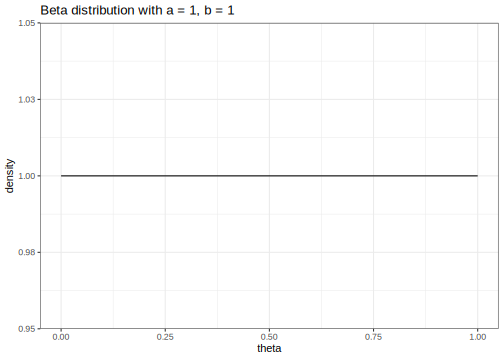
\includegraphics[width=0.48\linewidth]{bookdown_files/figure-latex/betas2-1} 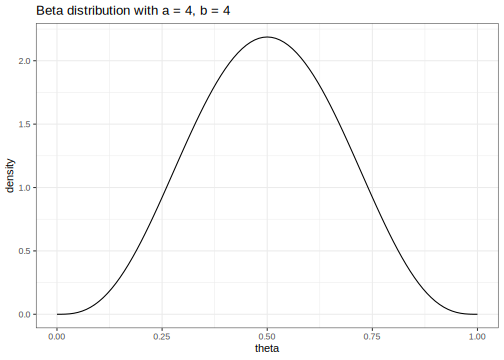
\includegraphics[width=0.48\linewidth]{bookdown_files/figure-latex/betas2-2} 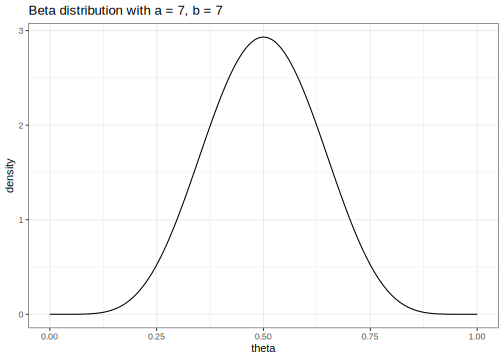
\includegraphics[width=0.48\linewidth]{bookdown_files/figure-latex/betas2-3} 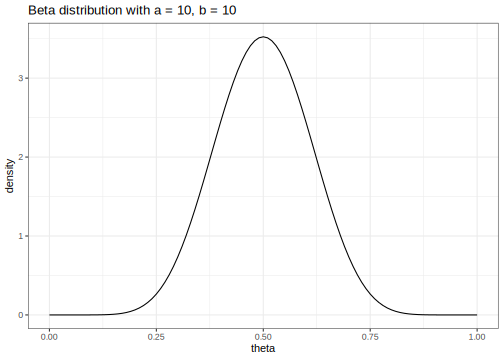
\includegraphics[width=0.48\linewidth]{bookdown_files/figure-latex/betas2-4} 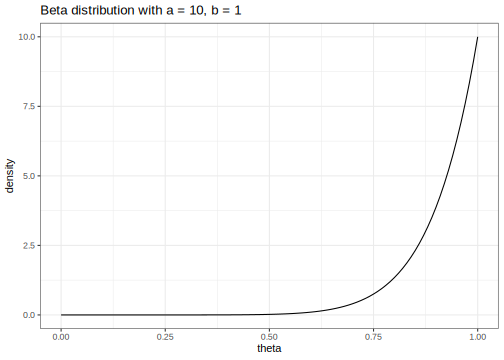
\includegraphics[width=0.48\linewidth]{bookdown_files/figure-latex/betas2-5} 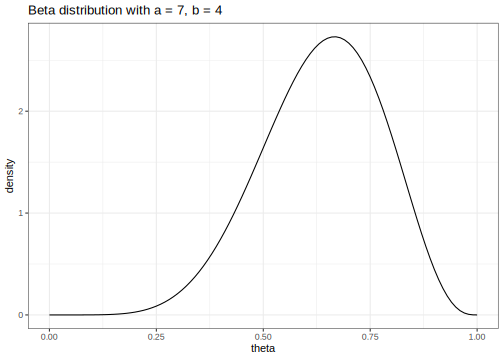
\includegraphics[width=0.48\linewidth]{bookdown_files/figure-latex/betas2-6} 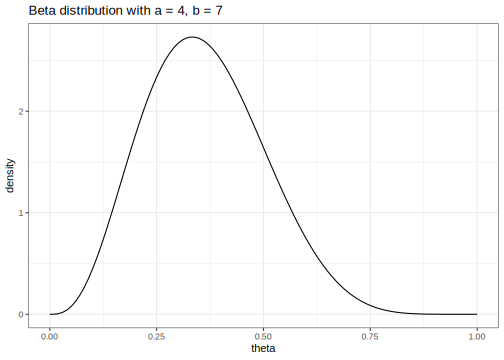
\includegraphics[width=0.48\linewidth]{bookdown_files/figure-latex/betas2-7} 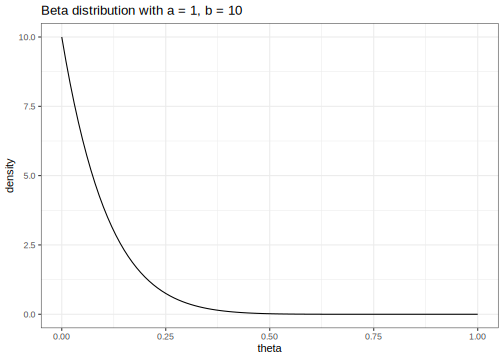
\includegraphics[width=0.48\linewidth]{bookdown_files/figure-latex/betas2-8} \caption{Examples of Beta distributions with different parameters.}\label{fig:betas2}
\end{figure}

As in the Binomial and Normal distributions that we saw in chapter 1,
one can analytically derive the formulas for the expectation and
variance of the Beta distribution. These are:

\begin{equation}
\operatorname{E}[X] = \frac{a}{a+b} \quad \operatorname{var}(X)=\frac {a \cdot b }{(a + b )^{2}(a + b +1)}
\label{eq:meanvar}
\end{equation}

As an example, choosing \(a=4\) and \(b=4\) would mean that the answer
``umbrella'' is as likely as a different answer, but we are relatively
unsure about this. We could express our uncertainty by computing the
region over which we are 95\% certain that the value of the parameter
lies; this is the \textbf{95\% credible interval}. For this, we would
use the \texttt{qbeta} function in R; the parameters \(a\) and \(b\) are
called \texttt{shape1} and \texttt{shape2} in \texttt{R}.

\begin{Shaded}
\begin{Highlighting}[]
\KeywordTok{qbeta}\NormalTok{(}\KeywordTok{c}\NormalTok{(}\FloatTok{0.025}\NormalTok{,}\FloatTok{0.975}\NormalTok{),}\DataTypeTok{shape1=}\DecValTok{4}\NormalTok{,}\DataTypeTok{shape2=}\DecValTok{4}\NormalTok{)}
\end{Highlighting}
\end{Shaded}

\begin{verbatim}
## [1] 0.184 0.816
\end{verbatim}

If we were to choose \(a=10\) and \(b=10\), we would still be assuming
that a priori the answer ``umbrella'' is just as likely as some other
answer, but now our prior uncertainty about this mean is lower, as the
95\% credible interval computed below shows.

\begin{Shaded}
\begin{Highlighting}[]
\KeywordTok{qbeta}\NormalTok{(}\KeywordTok{c}\NormalTok{(}\FloatTok{0.025}\NormalTok{,}\FloatTok{0.975}\NormalTok{),}\DataTypeTok{shape1=}\DecValTok{10}\NormalTok{,}\DataTypeTok{shape2=}\DecValTok{10}\NormalTok{)}
\end{Highlighting}
\end{Shaded}

\begin{verbatim}
## [1] 0.289 0.711
\end{verbatim}

In Figure \ref{fig:betas2}, we can see also the difference in
uncertainty in these two examples graphically.

Which prior should we choose? In a real data analysis problem, the
choice of prior would depend on what prior knowledge we want to bring
into the analysis. If we don't have much prior information, we could use
\(a=b=1\); this gives us a uniform prior. This kind of prior goes by
various names: \textbf{non-informative prior}, or \textbf{uninformative
prior}. By contrast, if we have a lot of prior knowledge and/or a strong
belief (e.g., based on a particular theory's predictions, or prior data)
that \(\theta\) has a particular range of plausible values, we can use a
different set of a,b values to reflect our belief about the parameter.
Notice in the above example that the larger our parameters a and b, the
narrower the spread of the distribution; i.e., the lower our uncertainty
about the mean value of the parameter.

For the moment, just for illustration, we choose the values \(a=4\) and
\(b=4\) for the Beta prior. Then, our prior for \(\theta\) is the
following Beta PDF:

\begin{equation}
p(\theta) = \frac{1}{B(4,4)} \theta^{3} (1-\theta)^{3}
\end{equation}

Having chosen a likelihood, and having defined a prior on \(\theta\), we
are ready to carry out our first Bayesian analysis to derive a posterior
distribution for \(\theta\).

\subsection{\texorpdfstring{Using Bayes' rule to compute the posterior
\(p(\theta|n,k)\)}{Using Bayes' rule to compute the posterior p(\textbackslash{}theta\textbar{}n,k)}}\label{using-bayes-rule-to-compute-the-posterior-pthetank}

Having specified the likelihood and the prior, we will now use Bayes'
rule to calculate \(p(\theta|n,k)\). Using Bayes' rule simply involves
replacing the Likelihood and the Prior we defined above into the
equation we saw earlier:

\begin{equation}
\hbox{Posterior} = \frac{\hbox{Likelihood} \cdot \hbox{Prior}}{\hbox{Marginal Likelihood}}
\end{equation}

Replace the terms for likelihood and prior into this equation:

\begin{equation}
p(\theta|n=10,k=8) = \frac{\left[\binom{10}{8} \theta^8 \cdot (1-\theta)^{2}\right]  \times \left[\frac{1}{B(4,4)} \times \theta^{3} (1-\theta)^{3}\right]}{p(k=8)}
\label{eq:betaunpost}
\end{equation}

where \(p(k=8)\) is \(\int_{0}^1 p(k=8|n,\theta) p(\theta)\, d\theta\).
This term will be a constant once the number of successes \(k\) is
known; this is the marginal likelihood we encountered in chapter 1. In
fact, once \(k\) is known, there are several constant values in the
above equation; they are constants because none of them depend on the
parameter of interest, \(\theta\). We can collect all of these together:

\begin{equation}
p(\theta|n=10,k=8) =   \left[ \frac{\binom{10}{8}}{B(4,4)\times p(k=8)} \right]   [\theta^8 (1-\theta)^{2} \times  \theta^{3} (1-\theta)^{3}]
\label{eq:betaunpost2}
\end{equation}

The first term that is in square brackets,
\(\frac{\binom{10}{8}}{B(4,4)\times p(k=8)}\), is all the constants
collected together, and is the normalizing constant we have seen before;
it makes the posterior distribution \(p(\theta|n=10,k=8)\) sum to one.
Since it is a constant, we can ignore it for now and focus on the two
other terms in the equation. Because we are ignoring the constant, we
will now say that the posterior is proportional to the right-hand side.

\begin{rmdnote} to-do: introduce the idea of an unnormalized
posterior here? see other suggestion elsewhere. \end{rmdnote}

\begin{equation}
p(\theta|n=10,k=8) \propto   [\theta^8 (1-\theta)^{2} \times \theta^{3} (1-\theta)^{3} ]
\label{eq:betaunpost3}
\end{equation}

A common way of writing the above equation is:

\begin{equation}
\hbox{Posterior} \propto \hbox{Likelihood} \times \hbox{Prior}
\end{equation}

Resolving the right-hand side now simply involves adding up the
exponents! In this example, computing the posterior really does boil
down to this simple addition operation on the exponents.

\begin{equation}
p(\theta|n=10,k=8) \propto   [\theta^{8+3} (1-\theta)^{2+3}] = \theta^{11} (1-\theta)^{5}
\label{eq:betaunpost4}
\end{equation}

The expression on the right-hand side corresponds to a Beta distribution
with parameters \(a=12\), and \(b=6\). This becomes evidence if we
rewrite the right-hand side such that it represents the core part of a
Beta PDF (see equation \eqref{eq:beta}). All that is missing is a
normalizing constant which would make the area under the curve sum to
one.

\begin{equation}
\theta^{11} (1-\theta)^{5} = \theta^{12-1} (1-\theta)^{6-1} 
\end{equation}

This core part of any PDF or PMF is called the kernel of that
distribution. Without a normalizing constant, the area under the curve
will not sum to one. Let's check this:

\begin{Shaded}
\begin{Highlighting}[]
\NormalTok{PostFun<-}\ControlFlowTok{function}\NormalTok{(theta)\{}
\NormalTok{  theta}\OperatorTok{^}\DecValTok{11} \OperatorTok{*}\StringTok{ }\NormalTok{(}\DecValTok{1}\OperatorTok{-}\NormalTok{theta)}\OperatorTok{^}\DecValTok{5}
\NormalTok{\}}
\NormalTok{(AUC<-}\KeywordTok{integrate}\NormalTok{(PostFun,}\DataTypeTok{lower=}\DecValTok{0}\NormalTok{,}\DataTypeTok{upper=}\DecValTok{1}\NormalTok{)}\OperatorTok{$}\NormalTok{value)}
\end{Highlighting}
\end{Shaded}

\begin{verbatim}
## [1] 0.0000135
\end{verbatim}

So the area under the curve (AUC) is not 1---the posterior that we
computed above is not a proper probability distribution.

All that is needed to make this into a proper probability distribution
is to include a normalizing constant, which, according to the definition
of the Beta distribution, would be \(B(12,6)\). This term is in fact the
integral we computed above.

\begin{equation}
p(\theta|n=10,k=8) = \frac{1}{B(12,6)} \theta^{12-1} (1-\theta)^{6-1} 
\end{equation}

Now, this function will sum to one:

\begin{Shaded}
\begin{Highlighting}[]
\NormalTok{PostFun<-}\ControlFlowTok{function}\NormalTok{(theta)\{}
\NormalTok{  theta}\OperatorTok{^}\DecValTok{11} \OperatorTok{*}\StringTok{ }\NormalTok{(}\DecValTok{1}\OperatorTok{-}\NormalTok{theta)}\OperatorTok{^}\DecValTok{5}\OperatorTok{/}\NormalTok{AUC}
\NormalTok{\}}
\KeywordTok{round}\NormalTok{(}\KeywordTok{integrate}\NormalTok{(PostFun,}\DataTypeTok{lower=}\DecValTok{0}\NormalTok{,}\DataTypeTok{upper=}\DecValTok{1}\NormalTok{)}\OperatorTok{$}\NormalTok{value,}\DecValTok{2}\NormalTok{)}
\end{Highlighting}
\end{Shaded}

\begin{verbatim}
## [1] 1
\end{verbatim}

\subsection{Summary of the procedure}\label{summary-of-the-procedure}

To summarize, we started with a Binomial likelihood, multiplied it with
the prior \(\theta \sim Beta(4,4)\), and obtained the posterior
\(p(\theta|n,k) \sim Beta(12,6)\). The constants were ignored when
carrying out the multiplication; we say that we computed the posterior
\textbf{up to proportionality}. Finally, we showed how, in this simple
example, the posterior can be rescaled to become a probability
distribution, by including a proportionality constant.

The above example is a case of a \textbf{conjugate} analysis: the
posterior on the parameter has the same form as the prior. The above
combination of likelihood and prior is called the Beta-Binomial
conjugate case. There are several other such combinations of Likelihoods
and Priors that yield a posterior that has the same PDF as the prior on
the parameter; some examples will appear in the exercises.

Formally, conjugacy is defined as follows:

\begin{quote}
DEFINITION Given the likelihood \(p(y| \theta)\), if the prior
\(p(\theta)\) results in a posterior \(y(\theta|y)\) that has the same
form as \(p(\theta)\), then we call \(p(\theta)\) a conjugate prior.
\end{quote}

For the Beta-Binomial case, we can derive a very general relationship
between the likelihood, prior, and posterior. Given the Binomial
likelihood up to proportionality (ignoring the constant)
\(\theta^k (1-\theta)^{n-k}\), and given the prior, also up to
proportionality, \(\theta^{a-1} (1-\theta)^{b-1}\), their product will
be:

\begin{equation}
\theta^k (1-\theta)^{n-k} \theta^{a-1} (1-\theta)^{b-1} = \theta^{a+k-1} (1-\theta)^{b+n-k-1} 
\end{equation}

Thus, given a \(Binomial(n,k|\theta)\) likelihood, and a \(Beta(a,b)\)
prior on \(\theta\), the posterior will be \(Beta(a+k,b+n-k)\).

\subsection{Visualizing the prior, likelihood, and the
posterior}\label{visualizing-the-prior-likelihood-and-the-posterior}

We established in the example above that the posterior is a Beta
distribution with parameters \(a=12\), and \(b = 6\). We visualize the
likelihood, prior, and the posterior alongside each other in
\ref{fig:postbeta-viz}.

\begin{figure}
\centering
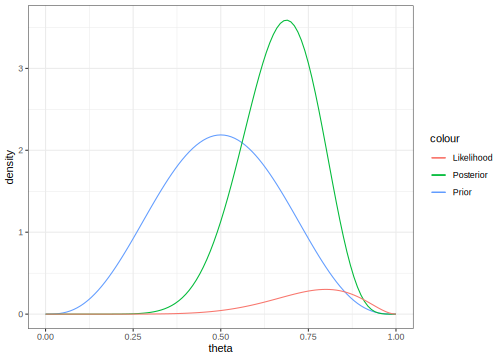
\includegraphics{bookdown_files/figure-latex/postbeta-viz-1.pdf}
\caption{\label{fig:postbeta-viz}The likelihood, prior, and posterior in the
Beta-Binomial example.}
\end{figure}

We can summarize the posterior distribution either graphically as we did
above, or summarize it by computing the mean and the variance. The mean
gives us an estimate of the Cloze probability of producing ``umbrella''
in that sentence (given the model, i.e., given the likelihood and
prior):

\begin{equation}
\operatorname{E}[\hat\theta] = \frac{12}{12+6}=0.67
\label{eq:meanPb}
\end{equation}

\begin{equation}
\operatorname{var}[\hat\theta]=\frac {12 \cdot 6 }{(12 + 6 )^{2}(12 + 6 +1)}= .01
\label{eq:varPb}
\end{equation}

We could also display the 95\% credible interval, the range over which
we are 95\% certain the true value of \(\theta\) lies, given the data
and model.

\begin{Shaded}
\begin{Highlighting}[]
\KeywordTok{qbeta}\NormalTok{(}\KeywordTok{c}\NormalTok{(}\FloatTok{0.025}\NormalTok{,}\FloatTok{0.975}\NormalTok{),}\DataTypeTok{shape1=}\DecValTok{12}\NormalTok{,}\DataTypeTok{shape2=}\DecValTok{6}\NormalTok{)}
\end{Highlighting}
\end{Shaded}

\begin{verbatim}
## [1] 0.440 0.858
\end{verbatim}

Typically, we would summarize the results of a Bayesian analysis by
displaying the posterior distribution of the parameter (or parameters)
graphically, along with the above summary statistics: the mean, the
standard deviation or variance, and the 95\% credible interval. You will
see many examples of such summaries later.

\subsection{The posterior distribution is a compromise between the prior
and the
likelihood}\label{the-posterior-distribution-is-a-compromise-between-the-prior-and-the-likelihood}

Just for the sake of illustration, let's take four different Beta
priors, each reflecting increasing certainty.

\begin{itemize}
\tightlist
\item
  Beta(a=2,b=2)
\item
  Beta(a=3,b=3)
\item
  Beta(a=6,b=6)
\item
  Beta(a=21,b=21)
\end{itemize}

Each prior reflects a belief that \(\theta=0.5\), with varying degrees
of (un)certainty. Given the general formula we developed above for the
Beta-Binomial case, we just need to plug in the likelihood and the prior
to get the posterior:

\begin{equation}
p(\theta | n,k) \propto p(k |n,\theta) p(\theta)
\end{equation}

The four corresponding posterior distributios would be:

\begin{equation}
p(\theta\mid k,n) \propto [\theta^{8} (1-\theta)^{2}] [\theta^{2-1}(1-\theta)^{2-1}] = \theta^{10-1} (1-\theta)^{4-1}
\end{equation}

\begin{equation}
p(\theta\mid k,n) \propto [\theta^{8} (1-\theta)^{2}] [\theta^{3-1}(1-\theta)^{3-1}] = \theta^{11-1} (1-\theta)^{5-1}
\end{equation}

\begin{equation}
p(\theta\mid k,n) \propto [\theta^{8} (1-\theta)^{2}] [\theta^{6-1}(1-\theta)^{6-1}] = \theta^{14-1} (1-\theta)^{8-1}
\end{equation}

\begin{equation}
p(\theta\mid k,n) \propto [\theta^{8} (1-\theta)^{2}] [\theta^{21-1}(1-\theta)^{21-1}] = \theta^{29-1} (1-\theta)^{23-1}
\end{equation}

We can easily visualize each of these triplets of priors, likelihoods
and posteriors. Use the Shiny app embedded below to visualize these
different prior-likelihood combinations and look at the posterior in
each case.

\begin{rmdnote} to-do: put in a shiny app that varies the a,b
parameters and the amount of data, to show how the posterior is
influenced by the data and the prior under different scenarios.
\end{rmdnote}

\begin{Shaded}
\begin{Highlighting}[]
\NormalTok{## this is just  a placeholder for the relevant shinyapp:}
\NormalTok{knitr}\OperatorTok{::}\KeywordTok{include_app}\NormalTok{(}\StringTok{"https://vasishth.shinyapps.io/AppTypeIPower"}\NormalTok{, }
  \DataTypeTok{height =} \StringTok{"500px"}\NormalTok{)}
\end{Highlighting}
\end{Shaded}

\begin{verbatim}
## Qt: Session management error: Could not open network socket
## TypeError: Attempting to change the setter of an unconfigurable property.
## TypeError: Attempting to change the setter of an unconfigurable property.
\end{verbatim}

\href{https://vasishth.shinyapps.io/AppTypeIPower}{\includegraphics{bookdown_files/figure-latex/shinybetabinomial-1.png}}

If you hold the likelihood function constant (held constant at
\(n=10, k=8\) in the above example), the tighter the prior, the greater
the extent to owhichh the posterior orients itself towards the prior. In
general, we can say the following about the likelihood-prior-posterior
relationship:

\begin{itemize}
\tightlist
\item
  The posterior distribution is a compromise between the prior and the
  likelihood.
\item
  For a given set of data, the greater the certainty in the prior, the
  more heavily the posterior will be influenced by the prior mean.
\item
  Conversely, for a given set of data, the greater the
  \textbf{un}certainty in the prior, the more heavily the posterior will
  be influenced by the likelihood.
\end{itemize}

Another important observation emerges if we increase the sample size
from \(10\) to, say, \(1,000,000\). Suppose we still get a sample mean
of \(0.8\) here, so that \(k=800,000\). Now, the posterior mean will be
influenced almost entirely by the sample mean. This is because, in the
general form for the posterior \(Beta(a+k,b+n-k)\) that we computed
above, the \(n\) and \(k\) become very large relative to the a, b
values, and dominate in determining the posterior mean.

Whenever we do a Bayesian analysis, it is good practice to check whether
the parameter you are interested in estimating is sensitive to the prior
specification. Such an investigation is called a \textbf{sensitivity
analysis}. Later in this book, we will see many examples of sensitivity
analyses in realistic data-analysis settings.

\subsection{Incremental knowledge gain using prior
knowledge}\label{incremental-knowledge-gain-using-prior-knowledge}

In the above example, we used an artificial example where we asked
\(10\) participants to complete the sentence shown at the beginning of
the chapter, and then we counted the number of times that they produced
``umbrella'' vs.~some other word as a continuation. Given 8 instances of
``umbrella'', and using a \(Beta(4,4)\) prior, we derived the posterior
to be \(Beta(12,6)\). We could now use this posterior as our prior for
the next study. Suppose that we were to carry out a second experiment,
again with 10 participants, and this time \(6\) produced ``umbrella''.
We could now use our new prior (Beta(12,6)) to obtain an updated
posterior. We have \(a=12, b=6, n=10, k=6\). This gives us as posterior:
\(Beta(a+k,b+n-k) = Beta(12+6,6+10-6)=Beta(18,10)\).

Now, if we were to pool all our data that we have from the two
experiments, then we would have as data \(n=20, k=14\). Suppose that we
keep our initial prior of \(a=4,b=4\). Then, our posterior would be
\(Beta(4+14,4+20-14)=Beta(18,10)\). This is exactly the same posterior
that we got when first analyzed the first \(10\) participants' data,
derived the posterior, and then used that posterior as a prior for the
next \(10\) participants' data.

This toy example illustrates an important point that has great practical
importance for cognitive science. One can incrementally gain information
about a research question by using information from previous studies and
deriving a posterior, and then use that posterior as a prior. For
practical examples from psycholinguistics showing how information can be
pooled from previous studies, see \citet{JaegerEngelmannVasishth2017}
and \citet{NicenboimRoettgeretal}. \citet{VasishthEngelmann2020}
illustrates an example of how the posterior from a previous study or
collection of studies can be used to compute the posterior derived from
new data. We return to this point in later chapters.

\begin{rmdnote} to-do: check that we do.
\end{rmdnote}

\section{Summary of concepts introduced in this
chapter}\label{summary-of-concepts-introduced-in-this-chapter-1}

In this chapter, we learnt how to use Bayes' rule in the specific case
of a Binomial likelihood, and a Beta prior on the \(\theta\) parameter
in the likelihood function. Our goal in any Bayesian analysis will
follow the path we took in this simple example: decide on an appropriate
likelihood function, decide on priors for all the parameters involved in
the likelihood function, and using this model (i.e., the likelihood and
the priors) derive the posterior distribution of each parameter. Then we
draw inferences about our research question based on the posterior
distribution of the parameter.

In the example discussed in this chapter, Bayesian analysis was easy.
This was because we considered the simple conjugate case of the
Beta-Binomial. In realistic data-analysis settings, our likelihood
function will be very complex, and many parameters will be involved.
Multiplying the likelihood function and the priors will become
mathematically difficult or impossible. For such situations, we use
computational methods to obtain samples from the posterior distributions
of the parameters.
\begin{rmdnote} to-do: add summary \end{rmdnote}
\section{Further reading}\label{further-reading-1}

to-do

\section{Exercises}\label{exercises-1}

\subsection{Exercise: Deriving Bayes'
rule}\label{exercise-deriving-bayes-rule}

Let A and B be two observable events. P(A) is the probability that A
occurs, and P(B) is the probability that B occurs. \(P(A|B)\) is the
conditional probability that A occurs given that B has happened.
\(P(A,B)\) is the joint probability of A and B both occurring.

You are given the definition of conditional probability:

\begin{equation}
P(A|B)= \frac{P(A,B)}{P(B)} \hbox{ where } P(B)>0
\end{equation}

Using the above definition, and using the fact that \(P(A,B)=P(B,A)\)
(i.e., the probability of A and B both occurring is the same as the
probability of B and A both occurring), derive an expression for
\(P(B|A)\). Show the steps clearly in the derivation.

\subsection{Exercise: Conjugate forms
1}\label{exercise-conjugate-forms-1}

\subsubsection{Computing the general form of a PDF for a
posterior}\label{computing-the-general-form-of-a-pdf-for-a-posterior}

Suppose you are given data \(k\) consisting of the number of successes,
coming from a \(Binomial(n,\theta)\) distribution. Example data are
shown below, generated with probability of success \(\theta=0.5\), just
for illustration:

\begin{Shaded}
\begin{Highlighting}[]
\NormalTok{## data:}
\NormalTok{k<-}\KeywordTok{rbinom}\NormalTok{(}\DataTypeTok{n=}\DecValTok{1}\NormalTok{,}\DataTypeTok{size=}\DecValTok{10}\NormalTok{,}\DataTypeTok{prob=}\FloatTok{0.5}\NormalTok{)}
\NormalTok{k}
\end{Highlighting}
\end{Shaded}

\begin{verbatim}
## [1] 6
\end{verbatim}

Here, \(n\) represents the number of trials, and \(k\) the number of
successes. The above code and output is just an example, and is no
longer relevant for the question below.

Given \(k\) successes in n trials coming from a Binomial distribution,
we define a \(Beta(a,b)\) prior on the parameter \(\theta\).

Write down the Beta distribution that represents the posterior, in terms
of \(a,b, n,\) and \(k\).

\subsubsection{Practical application}\label{practical-application}

We ask 10 yes/no questions from a participant, and the participant
returns 0 correct answers. We assume a Binomial likelihood function for
these data. Also assume a Beta(1,1) prior on the parameter \(\theta\),
which represents the probability of success. Use the result you derived
above to write down the posterior distribution of the \(\theta\)
parameter.

\subsection{Exercise: Conjugate forms
2}\label{exercise-conjugate-forms-2}

Suppose you have \(n\) independent and identically distributed data
points from a distribution that has the likelihood function
\(f(x|\theta)=\theta(1-\theta)^{\sum_{i=1}^n x_i}\), where the data
points \(x\) can have values 0,1,2,\dots. Let the prior on \(\theta\) be
Beta(a,b), a Beta distribution with parameters a,b. The posterior
distribution is a Beta distribution with parameters a* and b*. Determine
these parameters in terms of \(a\), \(b\), and \(\sum_{i=1}^n x_i\).

\subsection{Exercise: Conjugate forms
3}\label{exercise-conjugate-forms-3}

The Gamma distribution is defined in terms of the parameters a, b:
Ga(a,b). Given some data \(x\), the probability density function is:

\begin{equation}
Ga(x | a,b)=\frac{b^a x^{a-1} \exp\{-bx\}}{\Gamma(a)}
\end{equation}

We have data \(x_1,\dots, x_n\), with sample size \(n\) that is
exponentially distributed. The exponential likelihood function is:

\begin{equation}
p(x_1,\dots,x_n | \lambda)=\lambda^n \exp \{-\lambda \sum_{i=1}^n x_i \}
\end{equation}

It turns out that if we assume a Ga(a,b) prior distribution and the
above Exponential likelihood, the posterior distribution is a Gamma
distribution. In other words, the Gamma(a,b) prior on the \(\lambda\)
parameter in the Exponential distribution will be written:

\begin{equation}
Ga(\lambda | a,b)=\frac{b^a \lambda^{a-1} \exp\{-b\lambda\}}{\Gamma(a)}
\end{equation}

Find the parameters \(a'\) and \(b'\) of the posterior distribution.

\subsection{Exercise: Conjugate forms
4}\label{exercise-conjugate-forms-4}

\subsubsection{a. Computing the
posterior}\label{a.-computing-the-posterior}

This is a contrived example. Suppose we are modeling the number of times
that a speaker says the word ``I'' per day. This could be of interest if
we are studying, for example, how self-oriented a speaker is. The number
of times \(x\) that the word is uttered in over a particular time period
(here, one day) can be modeled by a Poisson distribution:

\begin{equation}
f(x\mid \theta) = \frac{\exp(-\theta) \theta^x}{x!}
\end{equation}

where the rate \(\theta\) is unknown, and the numbers of utterances of
the target word on each day are independent given \(\theta\).

We are told that the prior mean of \(\theta\) is 100 and prior variance
for \(\theta\) is 225. This information is based on the results of
previous studies on the topic. We will use the Gamma(a,b) density (see
previous question) as a prior for \(\theta\) because this is a conjugate
prior to the Poisson distribution.

\begin{itemize}
\tightlist
\item
  First, visualize the prior, a Gamma density prior for \(\theta\) based
  on the above information.
\end{itemize}

{[}Hint: Note that we know that for a Gamma density with parameters a,
b, the mean is \(\frac{a}{b}\) and the variance is \(\frac{a}{b^2}\).
Since we are given values for the mean and variance, we can solve for
a,b, which gives us the Gamma density.{]}

\begin{itemize}
\tightlist
\item
  Next, derive the posterior distribution of the parameter \(\theta\) up
  to proportionality, and write down the posterior distribution in terms
  of the parameters of a Gamma distribution.
\end{itemize}

\subsubsection{b. Practical application}\label{b.-practical-application}

Suppose we know that the number of ``I'' utterances from a particular
individual is \(115, 97, 79, 131\). Use the result you derived above to
obtain the posterior distribution. In other words, write down the a,b
parameters of the Gamma distribution representing the posterior
distribution of \(\theta\).

Plot the prior, likelihood, and the posterior alongside each other.

Now suppose you get one new data point: 200. Write down the updated
posterior (the a,b parameters of the Gamma distribution) given this new
data-point. Add the updated posterior to the plot you made above.

\part{Regression models}\label{part-regression-models}

\chapter{Computational Bayesian data analysis}\label{ch:compbda}

In the previous chapter, we learned how to analytically derive the
posterior distribution of the parameters in our model. In practice,
however, this is possible for only a very limited number of cases.
Although the numerator of the Bayes rule, the unnormalized posterior, is
easy to calculate (by multiplying the probability density/mass functions
analytically), the denominator, the marginal likelihood, requires us to
integrate the numerator; see \eqref{eq:bayesbrms}.

\begin{equation}
\begin{aligned}
p(\Theta|y) &= \cfrac{ p(y|\Theta) \cdot p(\Theta) }{p(y)}\\
p(\Theta|y) &= \cfrac{ p(y|\Theta) \cdot p(\Theta) }{\int_{\Theta} p(y|\Theta) \cdot p(\Theta) d\Theta }
\end{aligned}
\label{eq:bayesbrms}
\end{equation}

Unless we are dealing with conjugate distributions, the solution will be
extremely hard to derive or there will be no analytical solution. This
was the major bottleneck of Bayesian analysis in the past, and required
Bayesian practitioners to program an approximation method by themselves
before they could even begin the Bayesian analysis. Fortunately, many of
the probabilistic programming languages freely available today (see the
next section for a listing) allow us to define our models without having
to acquire expert knowledge about the relevant numerical techniques.

\section{Deriving the posterior through sampling}\label{sec:sampling}

Let's say that we want to derive the posterior of the model from
\ref{sec:analytical}, that is, the posterior distribution of the Cloze
probability of \emph{``umbrella''}, \(\theta\), given the following
data: a word (e.g., \emph{``umbrella''}) was answered 80 out of 100
times, and assuming a binomial distribution as the likelihood function,
and \(Beta(a=4,b=4)\) as a prior distribution for the Cloze probability.
If we have samples from the posterior distribution of \(\theta\),
instead of an analytically derived posterior distribution, given enough
samples we will have a good approximation of the real posterior
distribution. Getting samples from the posterior will be the only viable
option in the models that we will discuss in this book. By ``getting
samples'', we are talking about a situation analogous to when we use
\texttt{rbinom} or \texttt{rnorm} to obtain samples from a particular
distribution.

Thanks to probabilistic programming languages, it will be relatively
straightforward to get these samples, and we will discuss how we will do
it in more detail in the next section. For now let's assume that we used
some probabilistic programming language to obtain 20000 samples from the
posterior distribution of the Cloze probability, \(\theta\): 0.803,
0.675, 0.706, 0.749, 0.79, 0.704, 0.747, 0.762, 0.768, 0.813, 0.75,
0.787, 0.735, 0.781, 0.752, 0.785, 0.763, 0.716, 0.763, 0.742, \ldots{}
Figure \ref{fig:betapost} shows that the approximation of the posterior
looks quite similar to the real posterior. And in fact the difference
between the true and the approximated mean and variance are -0.0004 and
0.00002 respectively.





\begin{figure}
\centering
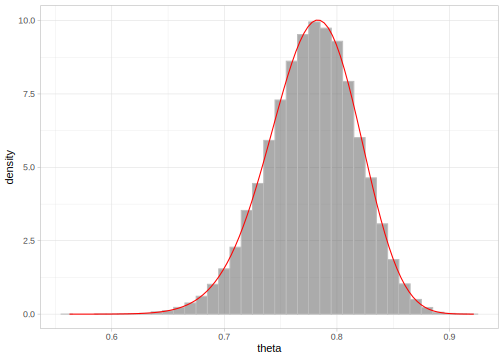
\includegraphics{bookdown_files/figure-latex/betapost-1.pdf}
\caption{\label{fig:betapost}Histogram of the samples of \(\theta\) from the posterior
distribution calculated through sampling in gray; density plot of the
exact posterior in red.}
\end{figure}

\subsection{\texorpdfstring{Bayesian Regression Models using `Stan':
brms}{Bayesian Regression Models using Stan: brms}}\label{bayesian-regression-models-using-stan-brms}

The surge in popularity of Bayesian statistics is closely tied to the
increase in computing power and the appearance of probabilistic
programming languages, such as WinBUGS \citep{lunn2000winbugs}, JAGS
\citep{plummer2016jags}, and more recently pymc3 \citep{Salvatier2016},
Turing \citep{turing}, and Stan \citep{carpenter2017stan}. These
statistical languages allow the user to define models without having to
deal (for the most part) with the complexities of the sampling process.
However, they require learning a new language since the user has to
fully specify the statistical model using a particular syntax.\footnote{The
  Python package pymc3 and the Julia package Turings are recent
  exceptions since they are fully integrated into the languages.}
Furthermore, some knowledge of the sampling process is needed to
correctly parameterize the models and to avoid convergences issues
(these topics will be covered in detail later in this book).

There are some alternatives that allow Bayesian inference in \texttt{R}
without having to fully specify the model ``by hand''. The packages
\texttt{rstanarm} \citep{rstanarm} and \texttt{brms} \citep{R-brms}
provide Bayesian equivalents of many popular R model-fitting functions,
such as (g)lmer \citep{lme4new}; both these packages use Stan for the
back-end estimation and sampling. JASP \citep{JASP2019} provides a
graphical user interface for both frequentist and Bayesian modeling, and
is intended to be an open-source alternative to SPSS.

We will focus on \texttt{brms} in the first part of the book. This is
because it can be useful for a smooth transition from frequentist models
to their Bayesian equivalents. Although \texttt{brms} is powerful enough
to satisfy the statistical needs of many cognitive scientists, it has
the added benefit that the Stan code can be inspected (with the
functions \texttt{make\_stancode} and \texttt{make\_standata}), allowing
the users to customize their models or learn from the code produced
internally by \texttt{brms} to eventually transition to write the models
entirely in Stan.

\subsubsection{A simple linear model: A single participant pressing a
button repeatedly}\label{sec:simplenormal}

We'll use the following example to illustrate the basic steps for
fitting a model. Let's say we have data from a participant repeatedly
pressing the space bar as fast as possible, without paying attention to
any stimuli. The data are reaction times in milliseconds in each trial.
We would like to know how long it takes to press a key when there is no
decision involved.

Let's model the data with the following assumptions:

\begin{enumerate}
\def\labelenumi{\arabic{enumi}.}
\tightlist
\item
  There is a true underlying time, \(\mu\), that the participant needs
  to press the space bar.
\item
  There is some noise in this process.
\item
  The noise is normally distributed (this assumption is questionable
  given that reaction times are generally skewed; we fix this assumption
  later).
\end{enumerate}

This means that the likelihood for each observation \(n\) will be:

\begin{equation}
\begin{aligned}
rt_n \sim Normal(\mu, \sigma)
\end{aligned}
\label{eq:rtlik}
\end{equation}

where \(n =1 \ldots N\), and \(rt\) is the dependent variable (reaction
times in milliseconds). The variable \(N\) indexes the total number of
data points. The letter \(\mu\) indicates the \emph{location} of the
normal distribution function; the location parameter shifts the
distribution left or right on the horizontal axis. For the normal
distribution, the location is also the mean of the distribution. The
letter \(\sigma\) indicates the \emph{scale} of the distribution; as the
scale decreases, the distribution gets narrower. This compressing
approaches a spike (all the probability mass in one point) as the scale
parameter goes to zero. For the normal distribution, the scale is also
its standard deviation.

For a frequentist model that will give us the maximum likelihood
estimate (the sample mean) of the time it takes to press the space bar,
this would be enough information to write the formula in \texttt{R},
\texttt{rt\ \textasciitilde{}\ 1}, and plug it into the function
\texttt{lm()} together with the data:
\texttt{lm(rt\ \textasciitilde{}\ 1,\ data)}. The meaning of the
\texttt{1} here is that there is no predictor associated with this
parameter, and \texttt{lm} will estimate the so-called intercept of the
model, in our case \(\mu\).

For a Bayesian model, we will also need to define priors for the two
parameters of our model. Let's say that we know for sure that the time
it takes to press a key will be positive and lower than a minute
(60000ms), but we don't want to make a commitment regarding which values
are more likely. We encode what we know about the noise in the task in
\(\sigma\): we know that this parameter must be positive and we'll
assume that any value below 2000ms is equally likely. These priors are
in general strongly discouraged because even when we know very little, a
flat (or very wide) prior will almost never be the best approximation of
what we know. We'll use them in this section for pedagogical purposes;
the next chapter will show more realistic uses of priors.

\begin{equation}
\begin{aligned}
\mu &\sim Uniform(0, 60000) \\
\sigma &\sim Uniform(0, 2000) 
\end{aligned}
\label{eq:rtpriors}
\end{equation}

We'll first load the data from \texttt{data/button\_press.csv}:

\begin{Shaded}
\begin{Highlighting}[]
\NormalTok{df_noreading_data <-}\StringTok{ }\KeywordTok{read_csv}\NormalTok{(}\StringTok{"./data/button_press.csv"}\NormalTok{)}
\NormalTok{df_noreading_data}
\end{Highlighting}
\end{Shaded}

\begin{verbatim}
## # A tibble: 361 x 2
##      rt trialn
##   <dbl>  <dbl>
## 1   141      1
## 2   138      2
## 3   128      3
## 4   132      4
## 5   126      5
## # ... with 356 more rows
\end{verbatim}

It is a good idea to look at the distribution of the data before doing
anything else; see Figure \ref{fig:m1visualize}. As we suspected, the
data look a bit skewed, but we ignore this for the moment.

\begin{Shaded}
\begin{Highlighting}[]
\KeywordTok{ggplot}\NormalTok{(df_noreading_data, }\KeywordTok{aes}\NormalTok{(rt)) }\OperatorTok{+}
\StringTok{  }\KeywordTok{geom_density}\NormalTok{() }\OperatorTok{+}
\StringTok{  }\KeywordTok{ggtitle}\NormalTok{(}\StringTok{"Button-press data"}\NormalTok{)}
\end{Highlighting}
\end{Shaded}

\begin{figure}
\centering
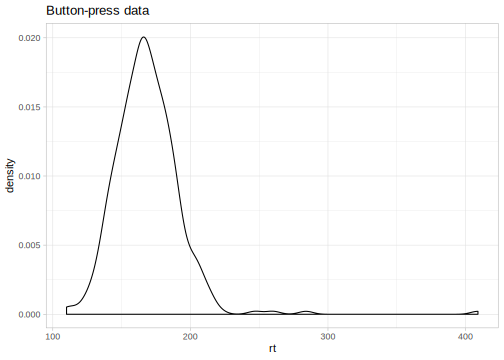
\includegraphics{bookdown_files/figure-latex/m1visualize-1.pdf}
\caption{\label{fig:m1visualize}Visualizing the data}
\end{figure}

\paragraph{\texorpdfstring{Specifying the model in
\texttt{brms}}{Specifying the model in brms}}\label{specifying-the-model-in-brms}

We'll fit the model defined by equations
\eqref{eq:rtlik}-\eqref{eq:rtpriors} with \texttt{brms} in the following
way; as we mentioned before the uniform distribution is not entirely
appropriate and we will ignore this warnings \emph{for now}:

\begin{Shaded}
\begin{Highlighting}[]
\NormalTok{fit_press <-}\StringTok{ }\KeywordTok{brm}\NormalTok{(rt }\OperatorTok{~}\StringTok{ }\DecValTok{1}\NormalTok{,}
  \DataTypeTok{data =}\NormalTok{ df_noreading_data,}
  \DataTypeTok{family =} \KeywordTok{gaussian}\NormalTok{(),}
  \DataTypeTok{prior =} \KeywordTok{c}\NormalTok{(}
    \KeywordTok{prior}\NormalTok{(}\KeywordTok{uniform}\NormalTok{(}\DecValTok{0}\NormalTok{, }\DecValTok{60000}\NormalTok{), }\DataTypeTok{class =}\NormalTok{ Intercept),}
    \KeywordTok{prior}\NormalTok{(}\KeywordTok{uniform}\NormalTok{(}\DecValTok{0}\NormalTok{, }\DecValTok{2000}\NormalTok{), }\DataTypeTok{class =}\NormalTok{ sigma)}
\NormalTok{  ),}
  \DataTypeTok{chains =} \DecValTok{4}\NormalTok{,}
  \DataTypeTok{iter =} \DecValTok{2000}\NormalTok{,}
  \DataTypeTok{warmup =} \DecValTok{1000}
\NormalTok{)}
\end{Highlighting}
\end{Shaded}

\begin{verbatim}
## Warning: It appears as if you have specified an upper bounded prior on a parameter that has no natural upper bound.
## If this is really what you want, please specify argument 'ub' of 'set_prior' appropriately.
## Warning occurred for prior 
## sigma ~ uniform(0, 2000)
\end{verbatim}

The \texttt{brms} code has some differences from a model fit with
\texttt{lm} (or \texttt{lmer} from the \texttt{lme4} package). At this
beginning stage, we'll focus on the following options:

\begin{enumerate}
\def\labelenumi{\arabic{enumi}.}
\tightlist
\item
  The term \texttt{family\ =\ gaussian()} makes explicit that the
  underlying likelihood function is a normal distribution (Gaussian and
  normal are synonyms) that is implicit in lm(er). Other linking
  functions are possible, exactly as in the glm(er) function.
\item
  The term \texttt{prior} takes as argument a vector of priors. Although
  this specification of priors is optional, the researcher should always
  explicitly specify each prior. Otherwise, \texttt{brms} will define a
  prior by default, which may or may not be appropriate for the research
  area.
\item
  The term \texttt{chains} refers to the number of independent runs for
  sampling (by default four).
\item
  The term \texttt{iter} refers to the number of iterations that the
  sampler makes to sample from the posterior distribution of each
  parameter (by default 2000).
\item
  The term \texttt{warmup} refers to the number of iterations from the
  start of sampling that are eventually discarded (by default half of
  \texttt{iter}).
\end{enumerate}

The last three options (together with \texttt{control} that was not used
before) determine the behavior of the sampler algorithm: the No-U-Turn
Sampler \citep[NUTS;][]{hoffmanNoUTurnSamplerAdaptively2014} extension
of Hamiltonian Monte Carlo
\citep{duaneHybridMonteCarlo1987, nealMCMCUsingHamiltonian2011}. We will
discuss sampling in more depth in chapter ??, but we explain here the
basic process.

\paragraph{Sampling and convergence in a
nutshell}\label{sec:convergencenut}

We start four chains independent from each other. Each chain
``searches'' for samples of the posterior in a multidimensional space,
where each parameter corresponds to a dimension, and the shape of this
space is determined by the priors and the likelihood. The chains start
in random locations and in each iteration they take one sample each. The
samples at the beginning do not belong to the posterior distribution.
Eventually, the chains end up in the vicinity of the posterior
distribution, and from that point onwards the samples will belong to the
posterior. That means that at the beginning the samples from the
different chains will be far from each other, but that \emph{at some
point} they will converge. While there are no guarantees that we are
running the chains for enough iterations, the default values of
\texttt{brms} (and Stan) are in many cases enough to achieve that, and
when they are not, we will receive warnings with recommendations. If the
chains converged to the same distribution, by removing the ``warmup''
(also called burn-in) samples--by default half of a total of 2000
iterations--, we make sure that we do not get samples from the path to
the posterior distribution. Figure \ref{fig:warmup} shows the path of
the chains from the warmup to the posterior and it is called a trace or
caterpillar plot. We show the warmup for illustration purposes, but
generally one should inspect the chains after the point where we assume
that convergence was achieved (i.e., after the dashed line). The chains
should look like one ``fat hairy caterpillar''. Compare the trace plot
of our model in Figure \ref{fig:warmup} with the traceplot of a model
that did not converge in Figure \ref{fig:warmup2}. Trace plots are,
however, not always that obvious. Traceplots might look fine, and still
the model may not have converged. Fortunately, Stan automatically runs
diagnostics with the information from the chains, and if there are no
warnings after fitting the model and the trace plots look fine, we can
be reasonably sure that the model converged and our samples are from the
true posterior distribution. However, we do need to run more than one
chain (preferably four), with a couple of thousands of iterations (at
least) so that the diagnostics will work.



\begin{figure}
\centering
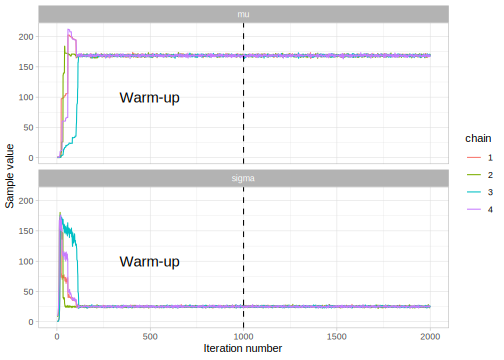
\includegraphics{bookdown_files/figure-latex/warmup-1.pdf}
\caption{\label{fig:warmup}Trace plot of our \texttt{brms} model}
\end{figure}



\begin{figure}
\centering
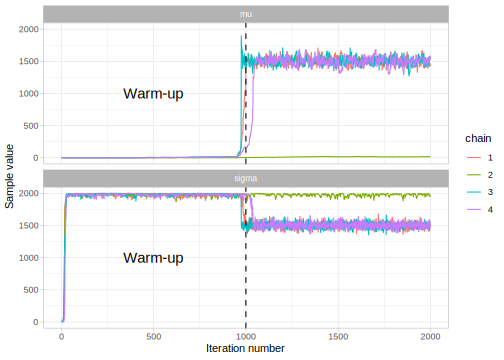
\includegraphics{bookdown_files/figure-latex/warmup2-1.pdf}
\caption{\label{fig:warmup2}Trace plot of a model that \textbf{did not} converge.}
\end{figure}

\paragraph{\texorpdfstring{Output of
\texttt{brms}}{Output of brms}}\label{output-of-brms}

If the model converged (i.e., if we didn't have any warning messages),
the output of the sampling process shows the samples of the posterior
distributions of each of the parameters:

\begin{Shaded}
\begin{Highlighting}[]
\KeywordTok{posterior_samples}\NormalTok{(fit_press) }\OperatorTok\StringTok{ }\KeywordTok{str}\NormalTok{() }
\end{Highlighting}
\end{Shaded}

\begin{verbatim}
## 'data.frame':    4000 obs. of  3 variables:
##  $ b_Intercept: num  170 168 169 169 168 ...
##  $ sigma      : num  22.9 23.7 26.4 26.3 24.2 ...
##  $ lp__       : num  -1691 -1689 -1689 -1689 -1688 ...
\end{verbatim}

Notice that \texttt{b\_Intercept} corresponds to our \(\mu\) and that
\texttt{lp} is not really part of the posterior, it's the density of the
unnormalized posterior for each iteration.

We can plot the histogram and the trace plot after the warmup:

\begin{Shaded}
\begin{Highlighting}[]
\KeywordTok{plot}\NormalTok{(fit_press)}
\end{Highlighting}
\end{Shaded}

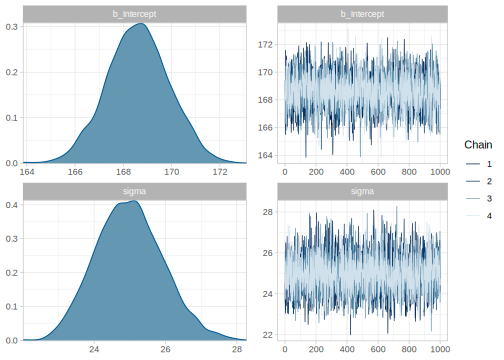
\includegraphics{bookdown_files/figure-latex/unnamed-chunk-65-1.pdf}

And \texttt{brms} provides a nice summary:

\begin{Shaded}
\begin{Highlighting}[]
\NormalTok{fit_press}
\CommentTok{# posterior_summary(fit_press) is also useful}
\end{Highlighting}
\end{Shaded}

\begin{verbatim}
##  Family: gaussian 
##   Links: mu = identity; sigma = identity 
## Formula: rt ~ 1 
##    Data: df_noreading_data (Number of observations: 361) 
## Samples: 4 chains, each with iter = 2000; warmup = 1000; thin = 1;
##          total post-warmup samples = 4000
## 
## Population-Level Effects: 
##           Estimate Est.Error l-95% CI u-95% CI Rhat Bulk_ESS Tail_ESS
## Intercept   168.63      1.31   166.09   171.15 1.00     3204     2635
## 
## Family Specific Parameters: 
##       Estimate Est.Error l-95% CI u-95% CI Rhat Bulk_ESS Tail_ESS
## sigma    25.04      0.96    23.25    27.00 1.00     3754     2382
## 
## Samples were drawn using sampling(NUTS). For each parameter, Bulk_ESS
## and Tail_ESS are effective sample size measures, and Rhat is the potential
## scale reduction factor on split chains (at convergence, Rhat = 1).
\end{verbatim}

Notice that the \texttt{Estimate} is just the mean of the posterior
sample, and CI are the 95\% quantiles:

\begin{Shaded}
\begin{Highlighting}[]
\KeywordTok{posterior_samples}\NormalTok{(fit_press)}\OperatorTok{$}\NormalTok{b_Intercept }\OperatorTok\StringTok{ }\KeywordTok{mean}\NormalTok{()}
\end{Highlighting}
\end{Shaded}

\begin{verbatim}
## [1] 169
\end{verbatim}

\begin{Shaded}
\begin{Highlighting}[]
\KeywordTok{posterior_samples}\NormalTok{(fit_press)}\OperatorTok{$}\NormalTok{b_Intercept }\OperatorTok\StringTok{ }\KeywordTok{quantile}\NormalTok{(}\KeywordTok{c}\NormalTok{(}\FloatTok{0.025}\NormalTok{, }\FloatTok{.975}\NormalTok{))}
\end{Highlighting}
\end{Shaded}

\begin{verbatim}
##  2.5% 97.5% 
##   166   171
\end{verbatim}

We see that we can fit our model without problems, and we get some
posterior distributions for our parameters. However, we should ask
ourselves the following questions:

\begin{enumerate}
\def\labelenumi{\arabic{enumi}.}
\tightlist
\item
  What information are the priors encoding? Do the priors make sense?
\item
  Does the likelihood assumed in the model make sense for the data?
\end{enumerate}

We'll try to answer these questions by looking at the \emph{Prior and
posterior predictive distributions}, and by doing sensitivity analyses
as described in the following sections.

\section{Prior predictive distribution}\label{sec:priorpred}

We had defined the following priors for our linear model:

\begin{equation}
\begin{aligned}
\mu &\sim Uniform(0, 60000) \\
\sigma &\sim Uniform(0, 2000) 
\label{eq:rtpriorsrepeated}
\end{aligned}
\end{equation}

These priors encode assumptions about the kind of data we would expect
to see in a future study. To understand these assumptions, we are going
to generate data from the model; such data, which is generated entirely
by the prior distributions, is called the prior predictive distribution.
Generating prior predictive distributions repeatedly helps us to check
whether the priors make sense. What we want to know here is, do the
priors generate realistic-looking data?

Formally, we want to know the density \(p(\cdot)\) of data points
\(y_{pred_1},\dots,y_{pred_N}\) from a dataset \(y_{pred}\) of length
\(N\), given a vector of priors \(\Theta\) and our likelihood
\(p(\cdot|\Theta)\); (in our example,
\(\Theta=\langle\mu,\sigma \rangle\)). The prior predictive density is
written as follows:

\begin{equation}
\begin{aligned}
p(y_{pred}) &= p(y_{pred_1},\dots,y_{pred_n})\\
&= \int_\Theta p(y_{pred_1}|\Theta)\cdot p(y_{pred_2}|\Theta)\cdots p(y_{pred_N}|\Theta) p(\Theta) \, d\Theta 
\end{aligned}
\end{equation}

In essence, we integrate out the vector of parameters, and we end up
with the probability distribution of possible datasets given the priors
and the likelihood we have defined, \emph{before we encounter any
observations}.

We can completely avoid doing the integration by generating samples from
the prior distribution instead. Notice here that each sample is an
imaginary or potential dataset.

Here is one way to generate prior predictive distributions:

Repeat the following many times:

\begin{enumerate}
\def\labelenumi{\arabic{enumi}.}
\tightlist
\item
  Take one sample from each of the priors.
\item
  Plug those samples in the likelihood and generate a dataset
  \(y_{pred_1},\ldots,y_{pred_n}\).
\end{enumerate}

We can create a function that does this:

\begin{Shaded}
\begin{Highlighting}[]
\NormalTok{normal_predictive_distribution <-}\StringTok{ }\ControlFlowTok{function}\NormalTok{(mu_samples, sigma_samples, N_obs) \{}
  \CommentTok{# empty data frame with headers:}
\NormalTok{  df_pred <-}\StringTok{ }\KeywordTok{tibble}\NormalTok{(}\DataTypeTok{trialn =} \KeywordTok{numeric}\NormalTok{(}\DecValTok{0}\NormalTok{),}
                    \DataTypeTok{rt_pred =} \KeywordTok{numeric}\NormalTok{(}\DecValTok{0}\NormalTok{),}
                    \DataTypeTok{iter =} \KeywordTok{numeric}\NormalTok{(}\DecValTok{0}\NormalTok{))}
  \CommentTok{# i iterates from 1 to the length of mu_samples,}
  \CommentTok{# which we assume is identical to }
  \CommentTok{# the length of the sigma_samples:}
  \ControlFlowTok{for}\NormalTok{ (i }\ControlFlowTok{in} \KeywordTok{seq_along}\NormalTok{(mu_samples)) \{}
\NormalTok{    mu <-}\StringTok{ }\NormalTok{mu_samples[i]}
\NormalTok{    sigma <-}\StringTok{ }\NormalTok{sigma_samples[i]}
\NormalTok{    df_pred <-}\StringTok{ }\KeywordTok{bind_rows}\NormalTok{(}
\NormalTok{      df_pred,}
      \KeywordTok{tibble}\NormalTok{(}\DataTypeTok{trialn =} \KeywordTok{seq_len}\NormalTok{(N_obs), }\CommentTok{#1, 2,... N_obs}
             \DataTypeTok{rt_pred =} \KeywordTok{rnorm}\NormalTok{(N_obs, mu, sigma),}
             \DataTypeTok{iter =}\NormalTok{ i)}
\NormalTok{    )}
\NormalTok{  \}}
\NormalTok{  df_pred}
\NormalTok{\}}
\end{Highlighting}
\end{Shaded}

The following code produces 1000 samples of the prior predictive
distribution of the model that we defined in \ref{sec:simplenormal}.
Although this approach works, it's quite slow (it takes about 5
seconds):

\begin{Shaded}
\begin{Highlighting}[]
\KeywordTok{tic}\NormalTok{()}
\NormalTok{N_samples <-}\StringTok{ }\DecValTok{1000}
\NormalTok{N_obs <-}\StringTok{ }\KeywordTok{nrow}\NormalTok{(df_noreading_data)}
\NormalTok{mu_samples <-}\StringTok{ }\KeywordTok{runif}\NormalTok{(N_samples, }\DecValTok{0}\NormalTok{, }\DecValTok{60000}\NormalTok{)}
\NormalTok{sigma_samples <-}\StringTok{ }\KeywordTok{runif}\NormalTok{(N_samples, }\DecValTok{0}\NormalTok{, }\DecValTok{2000}\NormalTok{)}

\NormalTok{prior_pred_slow <-}\StringTok{ }\KeywordTok{normal_predictive_distribution}\NormalTok{(}
  \DataTypeTok{mu_samples =}\NormalTok{ mu_samples,}
  \DataTypeTok{sigma_samples =}\NormalTok{ sigma_samples,}
  \DataTypeTok{N_obs =}\NormalTok{ N_obs}
\NormalTok{)}
\KeywordTok{toc}\NormalTok{()}
\end{Highlighting}
\end{Shaded}

\begin{verbatim}
## 3.678 sec elapsed
\end{verbatim}

\begin{Shaded}
\begin{Highlighting}[]
\NormalTok{prior_pred_slow}
\end{Highlighting}
\end{Shaded}

\begin{verbatim}
## # A tibble: 361,000 x 3
##   trialn rt_pred  iter
##    <dbl>   <dbl> <dbl>
## 1      1  39942.     1
## 2      2  42751.     1
## 3      3  39438.     1
## 4      4  40750.     1
## 5      5  39254.     1
## # ... with 360,995 more rows
\end{verbatim}

We can create a more efficient function in the following way using a
\texttt{map\_} function from \texttt{purrr} package. With this function,
we see an approximately 10-fold increase in speed. Notice that while the
distributions should be the same with both functions, the numbers that
we see in the tables won't be, due to the randomness in the process of
sampling.

\begin{Shaded}
\begin{Highlighting}[]
\NormalTok{normal_predictive_distribution_fast <-}\StringTok{ }\ControlFlowTok{function}\NormalTok{(mu_samples,}
\NormalTok{                                                sigma_samples,}
\NormalTok{                                                N_obs) \{}
  \CommentTok{# map_dfr works similarly to lapply, it essentially runs}
  \CommentTok{# a for-loop, and builds a dataframe with the output.}
  \CommentTok{# We iterate over the values of mu_samples and sigma_samples}
  \CommentTok{# simultaneously, and in each iteration we bind a new}
  \CommentTok{# data frame with N_obs observations.}
  \KeywordTok{map2_dfr}\NormalTok{(mu_samples, sigma_samples, }\ControlFlowTok{function}\NormalTok{(mu, sigma) \{}
    \KeywordTok{tibble}\NormalTok{(}
      \DataTypeTok{trialn =} \KeywordTok{seq_len}\NormalTok{(N_obs),}
      \DataTypeTok{rt_pred =} \KeywordTok{rnorm}\NormalTok{(N_obs, mu, sigma)}
\NormalTok{    )}
\NormalTok{  \}, }\DataTypeTok{.id =} \StringTok{"iter"}\NormalTok{) }\OperatorTok
\StringTok{    }\CommentTok{# .id is always a string and needs to be converted to a number}
\StringTok{    }\KeywordTok{mutate}\NormalTok{(}\DataTypeTok{iter =} \KeywordTok{as.numeric}\NormalTok{(iter))}
\NormalTok{\}}

\KeywordTok{tic}\NormalTok{()}
\NormalTok{prior_pred <-}\StringTok{ }\KeywordTok{normal_predictive_distribution_fast}\NormalTok{(}
  \DataTypeTok{mu_samples =}\NormalTok{ mu_samples,}
  \DataTypeTok{sigma_samples =}\NormalTok{ sigma_samples,}
\NormalTok{  N_obs)}
\KeywordTok{toc}\NormalTok{()}
\end{Highlighting}
\end{Shaded}

\begin{verbatim}
## 0.523 sec elapsed
\end{verbatim}

\begin{Shaded}
\begin{Highlighting}[]
\NormalTok{prior_pred}
\end{Highlighting}
\end{Shaded}

\begin{verbatim}
## # A tibble: 361,000 x 3
##    iter trialn rt_pred
##   <dbl>  <int>   <dbl>
## 1     1      1  39081.
## 2     1      2  42052.
## 3     1      3  39363.
## 4     1      4  40853.
## 5     1      5  39583.
## # ... with 360,995 more rows
\end{verbatim}

Figure \ref{fig:priorpred-simple} shows the first 18 samples of the
prior predictive distribution. These are 18 predicted datasets.




\begin{Shaded}
\begin{Highlighting}[]
\NormalTok{prior_pred }\OperatorTok
\StringTok{  }\KeywordTok{filter}\NormalTok{(iter }\OperatorTok{<=}\StringTok{ }\DecValTok{18}\NormalTok{) }\OperatorTok
\StringTok{  }\KeywordTok{ggplot}\NormalTok{(}\KeywordTok{aes}\NormalTok{(rt_pred)) }\OperatorTok{+}
\StringTok{  }\KeywordTok{geom_histogram}\NormalTok{() }\OperatorTok{+}
\StringTok{  }\KeywordTok{facet_wrap}\NormalTok{(}\OperatorTok{~}\NormalTok{iter, }\DataTypeTok{ncol =} \DecValTok{3}\NormalTok{)}
\end{Highlighting}
\end{Shaded}

\begin{figure}
\centering
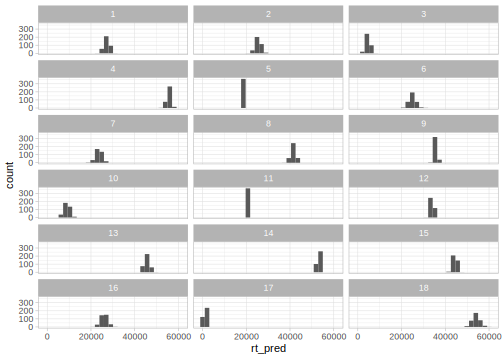
\includegraphics{bookdown_files/figure-latex/priorpred-simple-1.pdf}
\caption{\label{fig:priorpred-simple}Eighteen samples from the prior predictive
distribution of the model defined in \ref{sec:simplenormal}.}
\end{figure}

The prior predictive distribution in Figure \ref{fig:priorpred-simple}
shows prior datasets that are not realistic: Besides the fact that the
datasets show that reaction times distributions are symmetrical--and we
know that they are generally right-skewed--, some datasets present
reaction times that are unrealistically long, and worse yet, if we
inspect enough samples will find that a few datasets presents negative
press time values.

We can also look at the distribution of statistics here. Even if we
don't know beforehand what the data should look like, it's very likely
that we have some expectations for possible mean, minimum, or maximum
values.





\begin{Shaded}
\begin{Highlighting}[]
\NormalTok{prior_pred }\OperatorTok
\StringTok{  }\KeywordTok{group_by}\NormalTok{(iter) }\OperatorTok
\StringTok{  }\KeywordTok{summarize}\NormalTok{(}
    \DataTypeTok{min_rt =} \KeywordTok{min}\NormalTok{(rt_pred),}
    \DataTypeTok{max_rt =} \KeywordTok{max}\NormalTok{(rt_pred),}
    \DataTypeTok{average_rt =} \KeywordTok{mean}\NormalTok{(rt_pred)}
\NormalTok{  ) }\OperatorTok
\StringTok{  }\CommentTok{# we convert the previous data frame to a long one,}
\StringTok{  }\CommentTok{# where min_rt, max_rt, average_rt are possible values}
\StringTok{  }\CommentTok{# of the columns "stat"}
\StringTok{  }\KeywordTok{pivot_longer}\NormalTok{(}\DataTypeTok{cols =} \KeywordTok{ends_with}\NormalTok{(}\StringTok{"rt"}\NormalTok{),}
               \DataTypeTok{names_to =} \StringTok{"stat"}\NormalTok{,}
               \DataTypeTok{values_to =} \StringTok{"rt"}\NormalTok{) }\OperatorTok
\StringTok{  }\KeywordTok{ggplot}\NormalTok{(}\KeywordTok{aes}\NormalTok{(rt)) }\OperatorTok{+}
\StringTok{  }\KeywordTok{geom_histogram}\NormalTok{(}\DataTypeTok{binwidth =} \DecValTok{500}\NormalTok{) }\OperatorTok{+}
\StringTok{  }\KeywordTok{facet_wrap}\NormalTok{(}\OperatorTok{~}\NormalTok{stat, }\DataTypeTok{ncol =} \DecValTok{1}\NormalTok{)}
\end{Highlighting}
\end{Shaded}

\begin{figure}
\centering
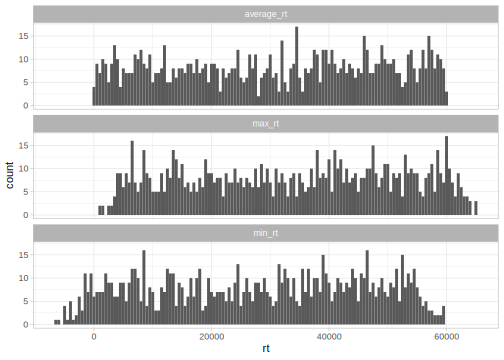
\includegraphics{bookdown_files/figure-latex/priorpred-stats-1.pdf}
\caption{\label{fig:priorpred-stats}Prior predictive distribution of averages,
maximum, and minimum value of the model defined in
\ref{sec:simplenormal}.}
\end{figure}

Figure \ref{fig:priorpred-stats} shows us that we used much less prior
information than what we really had: Our priors were encoding the
information that any mean between 0 and 60000 is expected, even though
we know that a value close to 0 or to 60000 would be extremely
surprising. It should be clear that this is because we are seeing the
effects of our uniform prior on \(\mu\). Similarly, maximum values are
quite ``uniform'', spanning a much wider range than what we would
expect. Finally, in the distribution of minimum values, we see that
negative observations are predicted. This might seem surprising (our
prior for \(\mu\) excluded negative values), but the reason we observe
negative values is that the prior is interpreted together with the
likelihood \citep{gelmanPriorCanOften2017}, and our likelihood is a
normal distribution, which will allow for negative samples no matter the
value of the parameter \(\mu\).

To summarize the above discussion, our priors are clearly not very
realistic given what we know about reaction times for such a button
pressing task. This raises the question: what priors should we have
chosen? In the next section, we consider this question.

\section{The influence of priors: sensitivity
analysis}\label{sec:sensitivity}

For most cases that we will encounter in this book, there are four main
classes of priors that we can choose from:

\subsection{Flat uninformative priors}\label{flat-uninformative-priors}

One option is to choose priors that are as uninformative as possible.
The idea behind this approach is to let the data ``speak for itself''
and to not bias the statistical inference with ``subjective'' priors.
There are several issues with this approach: First, the prior is as
subjective as the likelihood, and in fact, different choices of
likelihood might have a much stronger impact on the posterior than
different choices of priors. Second, uninformative priors are in general
unrealistic because they give equal weight to any value, ignoring the
fact that we do have some minimal information about our parameters of
interest, at the very least, the order of magnitude (reaction times will
be in milliseconds and not days, EEG signals some microvolts and not
volts, etc). Finally, uninformative priors make the sampling slower and
might lead to problems of convergence. Unless we have a large amount of
data, it would be wise to avoid them.

\subsection{Regularizing priors}\label{regularizing-priors}

If we don't have much prior information, and we have enough data (what
enough means here will presently become clear when we look at specific
examples), it is fine to use so-called \emph{regularizing priors}. These
are priors that downweight extreme values (that is, they provide
regularization), they are not very informative, and mostly let the
likelihood dominate in determining the posteriors. These priors are
theory-neutral; that is, they do not bias the parameters to values
supported by any theory. The idea behind this type of prior is to help
to stabilize computation. For many applications, they perform well, but
as we will see later, they tend to be problematic if we want to use
Bayes factors.

\subsection{Principled priors}\label{principled-priors}

The idea here is to have priors that encode all (or most of) the
theory-neutral information that we do have. Since we generally know how
our data do and do not look like, we can build priors that truly reflect
the properties of potential datasets.

\subsection{Informative priors}\label{informative-priors}

There are cases where we have a lot of prior knowledge, and not much
data. In general, unless we have \emph{very} good reasons for having
informative priors, we don't want our priors to have too much influence
on our posterior. An example where informative priors would be important
is when we are investigating a language-impaired population from which
we can't get many participants.

These four options constitute a continuum. The model from section
\ref{sec:simplenormal} falls between flat uninformative and regularizing
priors. The priors we used were flat but they allowed for values with at
least the right order of magnitude. In practical data analysis
situations, we are mostly going to choose priors that fall between
regularizing and principled.

\begin{rmdnote} to-do: I guess this section could be
completed. We should do a bit more justice to people advocating for
uninformative priors, and also refer to this idea of uninformative
priors that are invariant to transformations. SV: I think more
discussion would help beginners. We need to test this section out with
readers who are complete beginners. \end{rmdnote}

\section{Revisiting the button-pressing example with different
priors}\label{sec:revisit}

\begin{rmdnote} to-do: SV: could we show the posteriors from
the last and this model side by side using ridge plots?
\end{rmdnote}

What would happen if we use even wider priors for the model defined in
\ref{sec:simplenormal}? We could assume that every mean between
\(-10^{10}\) and \(10^{10}\) ms is equally likely. Regarding the
standard deviation, we could assume that any value between \(0\) and
\(10^{10}\) is equally likely. We keep the likelihood as it is, and we
encode the following priors:

\begin{equation}
\begin{aligned}
\mu &\sim Uniform(-10^{10}, 10^{10}) \\
\sigma &\sim Uniform(0,  10^{10}) 
\end{aligned}
\label{eq:rtpriorsflat}
\end{equation}

\begin{Shaded}
\begin{Highlighting}[]
\CommentTok{# We fit the model with the default setting of the sampler:}
\CommentTok{# 4 chains, 2000 iterations with half of them as warmup.}
\NormalTok{fit_press_unif <-}\StringTok{ }\KeywordTok{brm}\NormalTok{(rt }\OperatorTok{~}\StringTok{ }\DecValTok{1}\NormalTok{,}
  \DataTypeTok{data =}\NormalTok{ df_noreading_data,}
  \DataTypeTok{family =} \KeywordTok{gaussian}\NormalTok{(),}
  \DataTypeTok{prior =} \KeywordTok{c}\NormalTok{(}
    \KeywordTok{prior}\NormalTok{(}\KeywordTok{uniform}\NormalTok{(}\OperatorTok{-}\DecValTok{10}\OperatorTok{^}\DecValTok{10}\NormalTok{, }\DecValTok{10}\OperatorTok{^}\DecValTok{10}\NormalTok{), }\DataTypeTok{class =}\NormalTok{ Intercept),}
    \KeywordTok{prior}\NormalTok{(}\KeywordTok{uniform}\NormalTok{(}\DecValTok{0}\NormalTok{, }\DecValTok{10}\OperatorTok{^}\DecValTok{10}\NormalTok{), }\DataTypeTok{class =}\NormalTok{ sigma)}
\NormalTok{  )}
\NormalTok{)}
\end{Highlighting}
\end{Shaded}

\begin{verbatim}
## Warning: It appears as if you have specified an upper bounded prior on a parameter that has no natural upper bound.
## If this is really what you want, please specify argument 'ub' of 'set_prior' appropriately.
## Warning occurred for prior 
## sigma ~ uniform(0, 10^10)
\end{verbatim}

Notice that even with these extremely unrealistic priors the output of
the model is virtually identical!

\begin{Shaded}
\begin{Highlighting}[]
\NormalTok{fit_press_unif}
\end{Highlighting}
\end{Shaded}

\begin{verbatim}
##  Family: gaussian 
##   Links: mu = identity; sigma = identity 
## Formula: rt ~ 1 
##    Data: df_noreading_data (Number of observations: 361) 
## Samples: 4 chains, each with iter = 2000; warmup = 1000; thin = 1;
##          total post-warmup samples = 4000
## 
## Population-Level Effects: 
##           Estimate Est.Error l-95% CI u-95% CI Rhat Bulk_ESS Tail_ESS
## Intercept   168.65      1.33   166.07   171.26 1.00     4058     2933
## 
## Family Specific Parameters: 
##       Estimate Est.Error l-95% CI u-95% CI Rhat Bulk_ESS Tail_ESS
## sigma    24.99      0.94    23.24    26.88 1.00     3650     2985
## 
## Samples were drawn using sampling(NUTS). For each parameter, Bulk_ESS
## and Tail_ESS are effective sample size measures, and Rhat is the potential
## scale reduction factor on split chains (at convergence, Rhat = 1).
\end{verbatim}

What would happen if we had used very informative priors? We will assume
that mean values very close to 400 ms are the most likely, and that the
standard deviation of the reaction times is very close to 100. We
already know that this information is clearly wrong, because we have
already seen the output of some models. Notice that the \(Normal_+\)
notation indicates a normal distribution truncated in zero that only
allows positive values (Box \ref{thm:truncation} discusses this type of
distribution with more details):

\begin{equation}
\begin{aligned}
\mu &\sim Normal(400, 10) \\
\sigma &\sim Normal_+(100, 10) 
\end{aligned}
\label{eq:infrtpriors}
\end{equation}

\begin{Shaded}
\begin{Highlighting}[]
\NormalTok{fit_press_inf <-}\StringTok{ }\KeywordTok{brm}\NormalTok{(rt }\OperatorTok{~}\StringTok{ }\DecValTok{1}\NormalTok{,}
  \DataTypeTok{data =}\NormalTok{ df_noreading_data,}
  \DataTypeTok{family =} \KeywordTok{gaussian}\NormalTok{(),}
  \DataTypeTok{prior =} \KeywordTok{c}\NormalTok{(}
    \KeywordTok{prior}\NormalTok{(}\KeywordTok{normal}\NormalTok{(}\DecValTok{400}\NormalTok{, }\DecValTok{10}\NormalTok{), }\DataTypeTok{class =}\NormalTok{ Intercept),}
    \CommentTok{# brms knows that SD needs to be bounded by zero:}
    \KeywordTok{prior}\NormalTok{(}\KeywordTok{normal}\NormalTok{(}\DecValTok{100}\NormalTok{, }\DecValTok{10}\NormalTok{), }\DataTypeTok{class =}\NormalTok{ sigma)}
\NormalTok{  )}
\NormalTok{)}
\end{Highlighting}
\end{Shaded}

Even in this case, the likelihood mostly dominates and the new estimates
are just a couple of milliseconds away from our previous estimates:

\begin{Shaded}
\begin{Highlighting}[]
\NormalTok{fit_press_inf}
\end{Highlighting}
\end{Shaded}

\begin{verbatim}
##  Family: gaussian 
##   Links: mu = identity; sigma = identity 
## Formula: rt ~ 1 
##    Data: df_noreading_data (Number of observations: 361) 
## Samples: 4 chains, each with iter = 2000; warmup = 1000; thin = 1;
##          total post-warmup samples = 4000
## 
## Population-Level Effects: 
##           Estimate Est.Error l-95% CI u-95% CI Rhat Bulk_ESS Tail_ESS
## Intercept   172.93      1.45   170.19   175.83 1.00     2420     2352
## 
## Family Specific Parameters: 
##       Estimate Est.Error l-95% CI u-95% CI Rhat Bulk_ESS Tail_ESS
## sigma    26.08      1.05    24.20    28.22 1.00     2848     2473
## 
## Samples were drawn using sampling(NUTS). For each parameter, Bulk_ESS
## and Tail_ESS are effective sample size measures, and Rhat is the potential
## scale reduction factor on split chains (at convergence, Rhat = 1).
\end{verbatim}

This doesn't mean that priors never matter. When there is enough data,
the likelihood will dominate in determining the posterior distributions.
However, even in the cases where the likelihood dominates, more accurate
priors (i.e., more consistent with our real previous belief about the
data) will in general speed-up model convergence.

If we are not sure about the extent to which the posterior is influenced
by our priors, we can do a \emph{sensitivity analysis}: we try different
priors and either verify that the posterior doesn't change drastically,
or report how the posterior is affected by some specific priors
\citep[for a published example in psycholinguistics,
see][]{vasishthProcessingChineseRelative2013}. We will see later in this
book that \emph{sensitivity analysis} becomes crucial for reporting
Bayes factors (in chapter \ref{ch:bf}); even in cases where the choice
of priors does not affect the posterior distribution, it generally
affects the Bayes factor.

\section{Posterior predictive distribution}\label{sec:ppd}

The prior predictive distribution is a collection of datasets generated
from the model (the likelihood and the priors). After we have seen the
data and obtained the posterior distributions of the parameters, we can
now use the \emph{posterior distributions} to generate future data from
the model. In other words, given the posterior distributions of the
parameters of the model, the posterior predictive distribution shows how
future data might look like.

Once we have the posterior distribution \(p(\Theta\mid y)\), we can
derive the predictions based on this distribution:

\begin{equation}
p(y_{pred}\mid y ) = \int_\Theta p(y_{pred}, \Theta\mid y)\, d\Theta= \int_\Theta 
p(y_{pred}\mid \Theta,y)p(\Theta\mid y)\, d\Theta
\end{equation}

Assuming that past and future observations are conditionally independent
given \(\Theta\), i.e.,
\(p(y_{pred}\mid \Theta,y)= p(y_{pred}\mid \Theta)\), we can write:

\begin{equation}
p(y_{pred}\mid y )=\int_\Theta p(y_{pred}\mid \Theta) p(\Theta\mid y)\, d\Theta
\label{eq:postpp}
\end{equation}

Note that we are conditioning \(y_{pred}\) only on \(y\), we do not
condition on what we don't know (\(\Theta\)); we integrate out the
unknown parameters. This posterior predictive distribution is different
from the frequentist approach, which gives only a predictive
distribution of \(y_{pred}\) given our maximum likelihood estimate of
\(\theta\) (a point value). As with the prior predictive distribution,
we can avoid performing the integration explicitly by generating samples
from the posterior predictive distribution. We can use the same function
that we created before, \texttt{normal\_predictive\_distribution\_fast},
with the only difference in that instead of sampling \texttt{mu} and
\texttt{sigma} from the priors, we use samples from the posterior.

\begin{Shaded}
\begin{Highlighting}[]
\NormalTok{N_obs <-}\StringTok{ }\KeywordTok{nrow}\NormalTok{(df_noreading_data)}
\NormalTok{mu_samples <-}\StringTok{ }\KeywordTok{posterior_samples}\NormalTok{(fit_press)}\OperatorTok{$}\NormalTok{b_Intercept}
\NormalTok{sigma_samples <-}\StringTok{ }\KeywordTok{posterior_samples}\NormalTok{(fit_press)}\OperatorTok{$}\NormalTok{sigma}
\KeywordTok{normal_predictive_distribution_fast}\NormalTok{(}
  \DataTypeTok{mu_samples =}\NormalTok{ mu_samples,}
  \DataTypeTok{sigma_samples =}\NormalTok{ sigma_samples,}
\NormalTok{  N_obs}
\NormalTok{)}
\end{Highlighting}
\end{Shaded}

\begin{verbatim}
## # A tibble: 1,444,000 x 3
##    iter trialn rt_pred
##   <dbl>  <int>   <dbl>
## 1     1      1    149.
## 2     1      2    167.
## 3     1      3    127.
## 4     1      4    132.
## 5     1      5    203.
## # ... with 1,443,995 more rows
\end{verbatim}

There is a built-in function provided in \texttt{brms}, that will give
us the posterior predictive distribution:
\texttt{posterior\_predict(fit\_press)} provides the predicted reaction
times in a matrix, with the number of samples as rows and the number of
observations (data-points) as columns.

We can use the posterior predictive distribution to examine the
``descriptive adequacy'' of our models \citetext{\citealp[Chapter
6]{Gelman14}; \citealp{shiffrinSurveyModelEvaluation2008}}; these are
called posterior predictive checks, and what we want to establish here
is that the posterior predictive data look more or less similar to the
observed data. Achieving descriptive adequacy means that the current
data could have been generated by the model. While passing a test of
descriptive adequacy is not strong evidence in favor of a model, a major
failure in descriptive adequacy can be interpreted as strong evidence
against a model \citep{shiffrinSurveyModelEvaluation2008}. Thus,
posterior predictive checking is an important sanity check to assess
whether the model behavior is reasonable.

In many cases, we can simply use the plot functions from \texttt{brms}
and \texttt{bayesplot} that take the model as an argument for the
visualization of posterior predictive checks. For example, we can use
\texttt{pp\_check} to investigate how well the observed distribution of
reaction times fit our model based on some number (11 and 100) of
samples of the posterior predictive distributions; see figures
\ref{fig:normalppc} and \ref{fig:normalppc2}.




\begin{Shaded}
\begin{Highlighting}[]
\KeywordTok{pp_check}\NormalTok{(fit_press, }\DataTypeTok{nsamples =} \DecValTok{11}\NormalTok{, }\DataTypeTok{type =} \StringTok{"hist"}\NormalTok{)}
\end{Highlighting}
\end{Shaded}

\begin{figure}
\centering
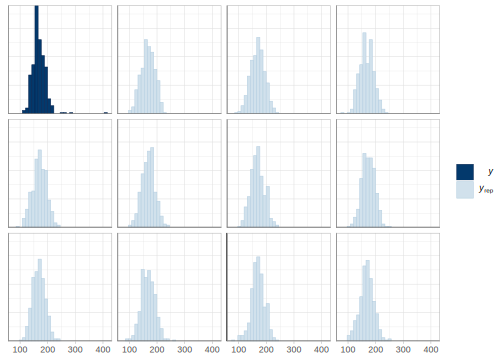
\includegraphics{bookdown_files/figure-latex/normalppc-1.pdf}
\caption{\label{fig:normalppc}Eleven samples from the posterior predictive
distribution of the model \texttt{fit\_press}.}
\end{figure}





\begin{Shaded}
\begin{Highlighting}[]
\KeywordTok{pp_check}\NormalTok{(fit_press, }\DataTypeTok{nsamples =} \DecValTok{100}\NormalTok{)}
\end{Highlighting}
\end{Shaded}

\begin{figure}
\centering
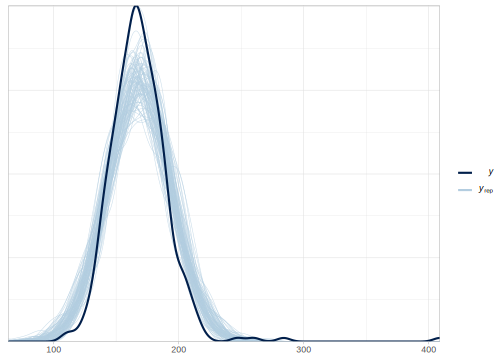
\includegraphics{bookdown_files/figure-latex/normalppc2-1.pdf}
\caption{\label{fig:normalppc2}Posterior predictive check that shows the fit of the
model \texttt{fit\_press} in comparison to datasets from the posterior
predictive distribution.}
\end{figure}

Notice that the real data is slightly skewed and has no values shorter
than 100 ms, while the predictive distributions are centered and
symmetrical; see figures \ref{fig:normalppc} and \ref{fig:normalppc2}.
This posterior predictive check shows a slight mismatch between the
observed and predicted data. Can we build a better model? We'll come
back to this issue in the next section.

\subsection{Comparing different
likelihoods}\label{comparing-different-likelihoods}

Since we know that the reaction times shouldn't be normally distributed,
we can choose a more realistic distribution for the likelihood. A good
candidate is the log-normal distribution since a variable (such as time)
that is log-normally distributed takes only positive real values and is
right skewed.

\subsection{The log-normal likelihood}\label{sec:lnfirst}

If \(y\) is log-normally distributed, this means that \(\log(y)\) is
normally distributed.\footnote{In fact, \(\log_e(y)\) or \(\ln(y)\), but
  we'll write it as just \(log()\)} Something important to notice is
that the log-normal distribution is again defined using \(\mu\) and
\(\sigma\), but these correspond to the mean and standard deviation of
the normally distributed logarithm of the data \(y\): \(\log(y)\). Thus,
when we model some data \(y\) using the log-normal likelihood, the
parameters \(\mu\) and \(\sigma\) are on a different scale than the data
\(y\).

We can create a log-normal distribution by exponentiating the samples of
a normal distribution. See Figure \ref{fig:logndemo}.

\begin{equation}
\begin{aligned}
\log(y) &\sim Normal( \mu, \sigma)\\
y &\sim \exp(Normal( \mu, \sigma)) \\
y &\sim LogNormal( \mu, \sigma)
\end{aligned}
\end{equation}

\begin{Shaded}
\begin{Highlighting}[]
\NormalTok{mu <-}\StringTok{ }\DecValTok{6}
\NormalTok{sigma <-}\StringTok{ }\FloatTok{0.5}
\NormalTok{N <-}\StringTok{ }\DecValTok{500000}
\CommentTok{# Generate N random samples from a log-normal distribution}
\NormalTok{sl <-}\StringTok{ }\KeywordTok{rlnorm}\NormalTok{(N, mu, sigma)}
\KeywordTok{ggplot}\NormalTok{(}\KeywordTok{tibble}\NormalTok{(}\DataTypeTok{samples =}\NormalTok{ sl), }\KeywordTok{aes}\NormalTok{(samples)) }\OperatorTok{+}
\StringTok{  }\KeywordTok{geom_histogram}\NormalTok{(}\DataTypeTok{binwidth =} \DecValTok{50}\NormalTok{) }\OperatorTok{+}
\StringTok{  }\KeywordTok{ggtitle}\NormalTok{(}\StringTok{"Log-normal distribution}\CharTok{\textbackslash{}n}\StringTok{"}\NormalTok{) }\OperatorTok{+}
\StringTok{  }\KeywordTok{coord_cartesian}\NormalTok{(}\DataTypeTok{ylim =} \KeywordTok{c}\NormalTok{(}\DecValTok{0}\NormalTok{, }\DecValTok{70000}\NormalTok{), }\DataTypeTok{xlim =} \KeywordTok{c}\NormalTok{(}\DecValTok{0}\NormalTok{, }\DecValTok{2000}\NormalTok{))}
\CommentTok{# Generate N random samples from a normal distribution,}
\CommentTok{# and then exponentiate them}
\NormalTok{sn <-}\StringTok{ }\KeywordTok{exp}\NormalTok{(}\KeywordTok{rnorm}\NormalTok{(N, mu, sigma))}
\KeywordTok{ggplot}\NormalTok{(}\KeywordTok{tibble}\NormalTok{(}\DataTypeTok{samples =}\NormalTok{ sn), }\KeywordTok{aes}\NormalTok{(samples)) }\OperatorTok{+}
\StringTok{  }\KeywordTok{geom_histogram}\NormalTok{(}\DataTypeTok{binwidth =} \DecValTok{50}\NormalTok{) }\OperatorTok{+}
\StringTok{  }\KeywordTok{ggtitle}\NormalTok{(}\StringTok{"Exponentiated samples of}\CharTok{\textbackslash{}n}\StringTok{a normal distribution"}\NormalTok{) }\OperatorTok{+}
\StringTok{    }\KeywordTok{coord_cartesian}\NormalTok{(}\DataTypeTok{ylim =} \KeywordTok{c}\NormalTok{(}\DecValTok{0}\NormalTok{, }\DecValTok{70000}\NormalTok{), }\DataTypeTok{xlim =} \KeywordTok{c}\NormalTok{(}\DecValTok{0}\NormalTok{, }\DecValTok{2000}\NormalTok{))}
\end{Highlighting}
\end{Shaded}

\begin{figure}
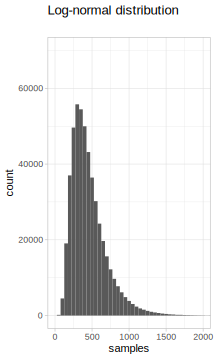
\includegraphics[width=0.48\linewidth]{bookdown_files/figure-latex/logndemo-1} 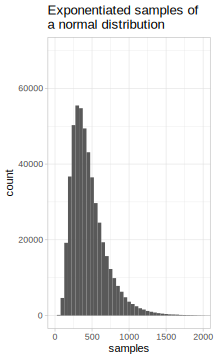
\includegraphics[width=0.48\linewidth]{bookdown_files/figure-latex/logndemo-2} \caption{Two log-normal distributions with the same parameters generated by either generating samples from a log-normal distribution or exponentiating samples from a normal distribution.}\label{fig:logndemo}
\end{figure}

\subsection{Re-fitting a single participant pressing a button repeatedly
with a log-normal likelihood}\label{sec:lognormal}

If we assume that reaction times are log-normally distributed, we'll
need to change our likelihood function as follows:

\begin{equation}
rt_n \sim LogNormal(\mu,\sigma)
\end{equation}

But now the scale of our priors needs to change! We'll continue with the
uniform priors for ease of exposition, even though, as we mentioned
earlier, these are not recommended.

\begin{equation}
\begin{aligned}
\mu &\sim Uniform(0, 8) \\
\sigma &\sim Uniform(0, 1) \\
\end{aligned}
\label{eq:logpriorsunif}
\end{equation}

Because the parameters are in a different scale than the dependent
variable, their interpretation changes and it is more complex than if we
were dealing with a linear model that assumes a normal likelihood
(location and scale do not coincide with the mean and standard deviation
of the log-normal):

\begin{itemize}
\tightlist
\item
  \emph{The location, \(\mu\)}: In our previous linear model, \(\mu\)
  represented the grand mean (or the grand median, or grand mode, since
  in a normal distribution the three coincide). But now, the grand mean
  needs to be calculated in the following way,
  \(\exp(\mu +\sigma ^{2}/2)\). Interestingly, the grand median will
  just be \(\exp(\mu)\). We could assume that the grand median,
  \(\exp(\mu)\), represents the underlying time it takes to press the
  space bar if there would be no noise, that is, if \(\sigma\) would be
  0. This also means that the prior of \(\mu\) is not in milliseconds,
  but in log(milliseconds).
\item
  \emph{The scale, \(\sigma\)}: This is the standard deviation of the
  normal distribution of \(\log(y)\). The standard deviation of a
  log-normal distribution with \emph{location} \(\mu\) and \emph{scale}
  \(\sigma\) will be
  \(\exp(\mu +\sigma ^{2}/2)\times \sqrt(\exp(\sigma^2)- 1)\). It's
  important to notice that, unlike the normal distribution, the spread
  of the log-normal distribution depends on both \(\mu\) and \(\sigma\).
\end{itemize}

To understand the meaning of our priors in the millisecond scale, we
need to take into account both the priors and the likelihood. We can do
this by generating a prior predictive distribution. Notice that we can
just exponentiate the samples produced by
\texttt{normal\_predictive\_distribution\_fast()} (or, alternatively, we
could have edited the function and replaced \texttt{rnorm} for
\texttt{rlnorm}).

\begin{Shaded}
\begin{Highlighting}[]
\NormalTok{N_samples <-}\StringTok{ }\DecValTok{1000}
\NormalTok{N_obs <-}\StringTok{ }\KeywordTok{nrow}\NormalTok{(df_noreading_data)}
\NormalTok{mu_samples <-}\StringTok{ }\KeywordTok{runif}\NormalTok{(N_samples, }\DecValTok{0}\NormalTok{, }\DecValTok{8}\NormalTok{)}
\NormalTok{sigma_samples <-}\StringTok{ }\KeywordTok{runif}\NormalTok{(N_samples, }\DecValTok{0}\NormalTok{, }\DecValTok{1}\NormalTok{)}
\NormalTok{prior_pred_ln <-}\StringTok{ }\KeywordTok{normal_predictive_distribution_fast}\NormalTok{(}
  \DataTypeTok{mu_samples =}\NormalTok{ mu_samples,}
  \DataTypeTok{sigma_samples =}\NormalTok{ sigma_samples,}
\NormalTok{  N_obs}
\NormalTok{) }\OperatorTok
\StringTok{  }\KeywordTok{mutate}\NormalTok{(}\DataTypeTok{rt_pred =} \KeywordTok{exp}\NormalTok{(rt_pred))}
\end{Highlighting}
\end{Shaded}

And then we plot the distribution of some representative statistics:





\begin{Shaded}
\begin{Highlighting}[]
\NormalTok{prior_pred_ln }\OperatorTok
\StringTok{  }\KeywordTok{group_by}\NormalTok{(iter) }\OperatorTok
\StringTok{  }\KeywordTok{summarize}\NormalTok{(}
    \DataTypeTok{min_rt =} \KeywordTok{min}\NormalTok{(rt_pred),}
    \DataTypeTok{max_rt =} \KeywordTok{max}\NormalTok{(rt_pred),}
    \DataTypeTok{average_rt =} \KeywordTok{mean}\NormalTok{(rt_pred),}
    \DataTypeTok{median_rt =} \KeywordTok{median}\NormalTok{(rt_pred)}
\NormalTok{  ) }\OperatorTok
\StringTok{  }\KeywordTok{pivot_longer}\NormalTok{(}\DataTypeTok{cols =} \KeywordTok{ends_with}\NormalTok{(}\StringTok{"rt"}\NormalTok{), }\DataTypeTok{names_to =} \StringTok{"stat"}\NormalTok{, }\DataTypeTok{values_to =} \StringTok{"rt"}\NormalTok{) }\OperatorTok
\StringTok{  }\KeywordTok{ggplot}\NormalTok{(}\KeywordTok{aes}\NormalTok{(rt)) }\OperatorTok{+}
\StringTok{  }\KeywordTok{scale_x_continuous}\NormalTok{(}\StringTok{"Reaction times in ms"}\NormalTok{,}
    \DataTypeTok{trans =} \StringTok{"log"}\NormalTok{, }\DataTypeTok{breaks =} \KeywordTok{c}\NormalTok{(}\FloatTok{0.001}\NormalTok{, }\DecValTok{1}\NormalTok{, }\DecValTok{10}\NormalTok{, }\DecValTok{100}\NormalTok{, }\DecValTok{1000}\NormalTok{, }\DecValTok{10000}\NormalTok{, }\DecValTok{100000}\NormalTok{)}
\NormalTok{  )}\OperatorTok{+}
\StringTok{  }\KeywordTok{geom_histogram}\NormalTok{() }\OperatorTok{+}
\StringTok{  }\KeywordTok{facet_wrap}\NormalTok{(}\OperatorTok{~}\NormalTok{stat, }\DataTypeTok{ncol =} \DecValTok{1}\NormalTok{)}
\end{Highlighting}
\end{Shaded}

\begin{figure}
\centering
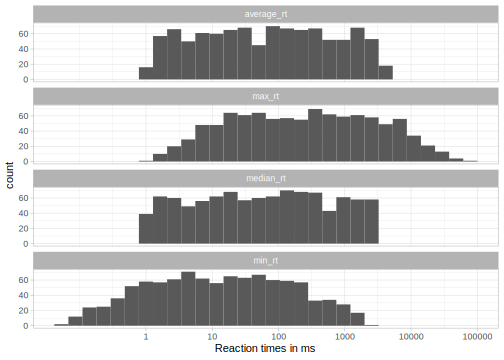
\includegraphics{bookdown_files/figure-latex/priorpredlogunif-1.pdf}
\caption{\label{fig:priorpredlogunif}Prior predictive distribution of averages,
maximum, and minimum value of the log-normal model with priors defined
in \eqref{eq:logpriorsunif}. Notice that the x-axis is log-transformed.}
\end{figure}

While we cannot generate negative values anymore, since \(\exp(\)any
number\() > 0\), and these priors might work, we can choose better
regularizing priors for our model, such as the following:

\begin{equation}
\begin{aligned}
\mu &\sim Normal(6, 1.5) \\
\sigma &\sim Normal_+(0, 1) \\
\end{aligned}
\label{eq:logpriorsnorm}
\end{equation}

Notice that while \(\mu\) can be negative, the dependent variable won't,
since the exponent of a negative value, \(\exp(\)some negative
value\()\), is always greater than \(0\). Even before generating the
prior predictive distributions, we can calculate the values within which
we are 95\% sure that the expected median of the observations will lie.
We do this by looking at what happens at two standard deviations away
from the mean of the \emph{prior}, \(\mu\), that is \(6 - 2\times 1.5\)
and \(6 + 2\times 1.5\), and exponentiating these values:

\begin{rmdnote} to-do: We should explain more the meaning of
location of the prior of sigma being 0. Maybe using
extraDistr::rtnorm(0,1,a=0) \end{rmdnote}

\begin{Shaded}
\begin{Highlighting}[]
\KeywordTok{c}\NormalTok{(}\DataTypeTok{lower =} \KeywordTok{exp}\NormalTok{(}\DecValTok{6} \OperatorTok{-}\StringTok{ }\DecValTok{2} \OperatorTok{*}\StringTok{ }\FloatTok{1.5}\NormalTok{),}
  \DataTypeTok{higher =} \KeywordTok{exp}\NormalTok{(}\DecValTok{6} \OperatorTok{+}\StringTok{ }\DecValTok{2} \OperatorTok{*}\StringTok{ }\FloatTok{1.5}\NormalTok{))}
\end{Highlighting}
\end{Shaded}

\begin{verbatim}
##  lower higher 
##   20.1 8103.1
\end{verbatim}

This means that our prior for \(\mu\) is still not too informative
(these are medians; the actual values generated by the distribution can
be much more spread out). We plot the distribution of some
representative statistics in Figure \ref{fig:priorpredlognorm}.





\begin{Shaded}
\begin{Highlighting}[]
\NormalTok{N_samples <-}\StringTok{ }\DecValTok{1000}
\NormalTok{N_obs <-}\StringTok{ }\KeywordTok{nrow}\NormalTok{(df_noreading_data)}
\NormalTok{mu_samples <-}\StringTok{ }\KeywordTok{rnorm}\NormalTok{(N_samples, }\DecValTok{6}\NormalTok{, }\FloatTok{1.5}\NormalTok{)}
\NormalTok{sigma_samples <-}\StringTok{ }\KeywordTok{rtnorm}\NormalTok{(N_samples, }\DecValTok{0}\NormalTok{, }\DecValTok{1}\NormalTok{, }\DataTypeTok{a =} \DecValTok{0}\NormalTok{)}
\NormalTok{prior_pred_ln_better <-}\StringTok{ }\KeywordTok{normal_predictive_distribution_fast}\NormalTok{(}
  \DataTypeTok{mu_samples =}\NormalTok{ mu_samples,}
  \DataTypeTok{sigma_samples =}\NormalTok{ sigma_samples,}
\NormalTok{  N_obs) }\OperatorTok
\StringTok{  }\KeywordTok{mutate}\NormalTok{(}\DataTypeTok{rt_pred =} \KeywordTok{exp}\NormalTok{(rt_pred))}
  

\NormalTok{prior_pred_ln_better }\OperatorTok
\StringTok{  }\KeywordTok{group_by}\NormalTok{(iter) }\OperatorTok
\StringTok{  }\KeywordTok{summarize}\NormalTok{(}
    \DataTypeTok{min_rt =} \KeywordTok{min}\NormalTok{(rt_pred),}
    \DataTypeTok{max_rt =} \KeywordTok{max}\NormalTok{(rt_pred),}
    \DataTypeTok{average_rt =} \KeywordTok{mean}\NormalTok{(rt_pred),}
    \DataTypeTok{median_rt =} \KeywordTok{median}\NormalTok{(rt_pred)}
\NormalTok{  ) }\OperatorTok
\StringTok{ }\KeywordTok{pivot_longer}\NormalTok{(}\DataTypeTok{cols =} \KeywordTok{ends_with}\NormalTok{(}\StringTok{"rt"}\NormalTok{),}
              \DataTypeTok{names_to =} \StringTok{"stat"}\NormalTok{, }\DataTypeTok{values_to =} \StringTok{"rt"}\NormalTok{) }\OperatorTok
\StringTok{  }\KeywordTok{ggplot}\NormalTok{(}\KeywordTok{aes}\NormalTok{(rt)) }\OperatorTok{+}
\StringTok{  }\KeywordTok{scale_x_continuous}\NormalTok{(}\DataTypeTok{trans =} \StringTok{"log"}\NormalTok{, }\DataTypeTok{breaks =} \KeywordTok{c}\NormalTok{(}\FloatTok{0.001}\NormalTok{, }\DecValTok{1}\NormalTok{, }\DecValTok{100}\NormalTok{, }\DecValTok{1000}\NormalTok{, }\DecValTok{10000}\NormalTok{, }\DecValTok{100000}\NormalTok{)) }\OperatorTok{+}
\StringTok{  }\KeywordTok{geom_histogram}\NormalTok{() }\OperatorTok{+}
\StringTok{  }\KeywordTok{facet_wrap}\NormalTok{(}\OperatorTok{~}\NormalTok{stat, }\DataTypeTok{ncol =} \DecValTok{1}\NormalTok{) }\OperatorTok{+}
\StringTok{  }\KeywordTok{coord_cartesian}\NormalTok{(}\DataTypeTok{xlim =} \KeywordTok{c}\NormalTok{(}\FloatTok{0.001}\NormalTok{, }\DecValTok{300000}\NormalTok{))}
\end{Highlighting}
\end{Shaded}

\begin{figure}
\centering
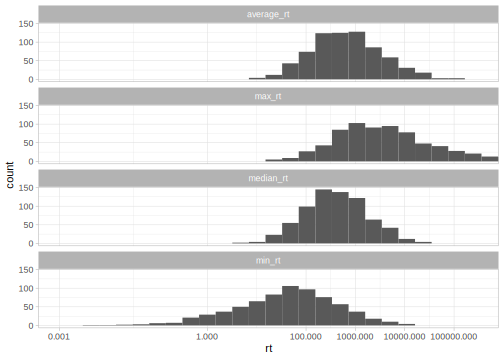
\includegraphics{bookdown_files/figure-latex/priorpredlognorm-1.pdf}
\caption{\label{fig:priorpredlognorm}Prior predictive distribution of averages,
maximum, and minimum value of the log-normal model with priors defined
in \eqref{eq:logpriorsnorm}. Notice that the x-axis is log-transformed.}
\end{figure}

We see that the priors that we are using are still too uninformative.
The tails of the prior predictive distributions that correspond to our
normal priors shown in Figure \ref{fig:priorpredlognorm} are even
further to the right reaching more extreme values than for the
predictive distributions generated by uniform priors shown in Figure
\ref{fig:priorpredlogunif}. Our new priors are still far from perfectly
encoding our prior knowledge. We could do more iterations of choosing
priors and generating prior predictive distributions until we have
priors that generate realistic data. However, for most cases, priors
that generate data whose statistics (mean, median, min, max, etc.) lie
roughly in the correct order of magnitude are going to be acceptable.

We can fit the model now, but notice that we need to specify that the
family is \texttt{lognormal()}. In our first example, we had used the
family \texttt{gaussian()}.

\begin{Shaded}
\begin{Highlighting}[]
\NormalTok{fit_press_ln <-}\StringTok{ }\KeywordTok{brm}\NormalTok{(rt }\OperatorTok{~}\StringTok{ }\DecValTok{1}\NormalTok{,}
  \DataTypeTok{data =}\NormalTok{ df_noreading_data,}
  \DataTypeTok{family =} \KeywordTok{lognormal}\NormalTok{(),}
  \DataTypeTok{prior =} \KeywordTok{c}\NormalTok{(}
    \KeywordTok{prior}\NormalTok{(}\KeywordTok{normal}\NormalTok{(}\DecValTok{6}\NormalTok{, }\FloatTok{1.5}\NormalTok{), }\DataTypeTok{class =}\NormalTok{ Intercept),}
    \KeywordTok{prior}\NormalTok{(}\KeywordTok{normal}\NormalTok{(}\DecValTok{0}\NormalTok{, }\DecValTok{1}\NormalTok{), }\DataTypeTok{class =}\NormalTok{ sigma)}
\NormalTok{  )}
\NormalTok{)}
\end{Highlighting}
\end{Shaded}

When we look at the summary of the posterior, the parameters are in
log-scale:

\begin{Shaded}
\begin{Highlighting}[]
\NormalTok{fit_press_ln}
\end{Highlighting}
\end{Shaded}

\begin{verbatim}
##  Family: lognormal 
##   Links: mu = identity; sigma = identity 
## Formula: rt ~ 1 
##    Data: df_noreading_data (Number of observations: 361) 
## Samples: 4 chains, each with iter = 2000; warmup = 1000; thin = 1;
##          total post-warmup samples = 4000
## 
## Population-Level Effects: 
##           Estimate Est.Error l-95% CI u-95% CI Rhat Bulk_ESS Tail_ESS
## Intercept     5.12      0.01     5.10     5.13 1.00     3654     2838
## 
## Family Specific Parameters: 
##       Estimate Est.Error l-95% CI u-95% CI Rhat Bulk_ESS Tail_ESS
## sigma     0.13      0.00     0.13     0.14 1.00     2956     2738
## 
## Samples were drawn using sampling(NUTS). For each parameter, Bulk_ESS
## and Tail_ESS are effective sample size measures, and Rhat is the potential
## scale reduction factor on split chains (at convergence, Rhat = 1).
\end{verbatim}

If we want to know how long does it take to press the space bar in
milliseconds, we need to transform the \(\mu\) (or \texttt{Intercept} in
the model) to milliseconds. Since we know that the median of the
log-normal distribution is \(exp(\mu)\), we do the following to
calculate an estimate in milliseconds:

\begin{Shaded}
\begin{Highlighting}[]
\NormalTok{estimate_ms <-}\StringTok{ }\KeywordTok{exp}\NormalTok{(}\KeywordTok{posterior_samples}\NormalTok{(fit_press_ln)}\OperatorTok{$}\NormalTok{b_Intercept)}
\end{Highlighting}
\end{Shaded}

If we want to know the mean and 95\% credible interval, we do the
following:

\begin{Shaded}
\begin{Highlighting}[]
\KeywordTok{c}\NormalTok{(}\DataTypeTok{mean =} \KeywordTok{mean}\NormalTok{(estimate_ms), }\KeywordTok{quantile}\NormalTok{(estimate_ms, }\DataTypeTok{probs =} \KeywordTok{c}\NormalTok{(.}\DecValTok{025}\NormalTok{, }\FloatTok{.975}\NormalTok{)))}
\end{Highlighting}
\end{Shaded}

\begin{verbatim}
##  mean  2.5% 97.5% 
##   167   165   169
\end{verbatim}

We can now verify whether our predicted datasets look similar to the
real dataset. See Figure \ref{fig:lognppc}; compare this with the
earlier Figure \ref{fig:normalppc2}.




\begin{Shaded}
\begin{Highlighting}[]
\KeywordTok{pp_check}\NormalTok{(fit_press_ln, }\DataTypeTok{nsamples =} \DecValTok{100}\NormalTok{)}
\end{Highlighting}
\end{Shaded}

\begin{figure}
\centering
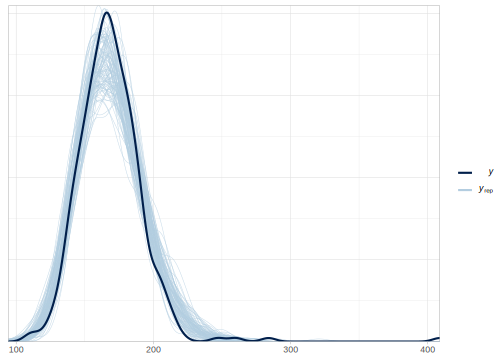
\includegraphics{bookdown_files/figure-latex/lognppc-1.pdf}
\caption{\label{fig:lognppc}Posterior predictive distribution of
\texttt{fit\_noreading\_ln}}
\end{figure}

\emph{Are the posterior predicted data now more similar to the real
data, compared to the case where we had a Normal likelihood?}

It seems so, but it's not easy to tell. Another way to examine this
would be to look at the distribution of summary statistics. We compare
the distribution of representative summary statistics for the datasets
generated by different models and compare them to the observed
statistics. We suspect that the normal distribution would generate
reaction times that are too fast (since it's symmetrical) and that the
log-normal distribution may capture the long tail better than the normal
model. Based on our hunch, we compute the distribution of minimum and
maximum values for the posterior predictive distributions, and we
compare them with the minimum and maximum value respectively in the
data.

\begin{Shaded}
\begin{Highlighting}[]
\KeywordTok{pp_check}\NormalTok{(fit_press, }\DataTypeTok{type =} \StringTok{"stat"}\NormalTok{, }\DataTypeTok{stat =} \StringTok{"min"}\NormalTok{) }\OperatorTok{+}\StringTok{ }\KeywordTok{ggtitle}\NormalTok{(}\StringTok{"Normal model"}\NormalTok{)}
\KeywordTok{pp_check}\NormalTok{(fit_press_ln, }\DataTypeTok{type =} \StringTok{"stat"}\NormalTok{, }\DataTypeTok{stat =} \StringTok{"min"}\NormalTok{) }\OperatorTok{+}\StringTok{ }\KeywordTok{ggtitle}\NormalTok{(}\StringTok{"Log-normal model"}\NormalTok{)}
\end{Highlighting}
\end{Shaded}

\begin{figure}
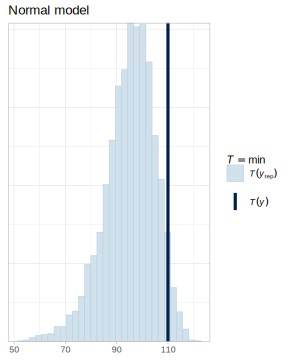
\includegraphics[width=0.45\linewidth]{bookdown_files/figure-latex/ppcheckmin-1} 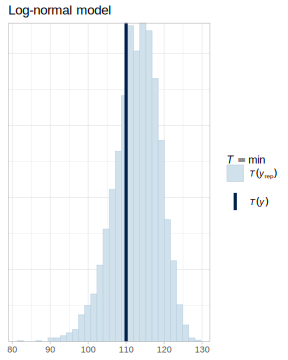
\includegraphics[width=0.45\linewidth]{bookdown_files/figure-latex/ppcheckmin-2} \caption{Distribution of minimum values in a posterior predictive check. The minimum in the data is 110 ms.}\label{fig:ppcheckmin}
\end{figure}

\begin{Shaded}
\begin{Highlighting}[]
\KeywordTok{pp_check}\NormalTok{(fit_press, }\DataTypeTok{type =} \StringTok{"stat"}\NormalTok{, }\DataTypeTok{stat =} \StringTok{"max"}\NormalTok{) }\OperatorTok{+}\StringTok{ }\KeywordTok{ggtitle}\NormalTok{(}\StringTok{"Normal model"}\NormalTok{)}
\KeywordTok{pp_check}\NormalTok{(fit_press_ln, }\DataTypeTok{type =} \StringTok{"stat"}\NormalTok{, }\DataTypeTok{stat =} \StringTok{"max"}\NormalTok{) }\OperatorTok{+}\StringTok{ }\KeywordTok{ggtitle}\NormalTok{(}\StringTok{"Log-normal model"}\NormalTok{)}
\end{Highlighting}
\end{Shaded}

\begin{figure}
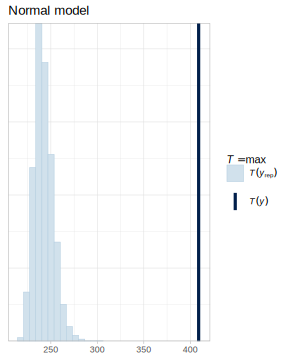
\includegraphics[width=0.45\linewidth]{bookdown_files/figure-latex/ppcheckmax-1} 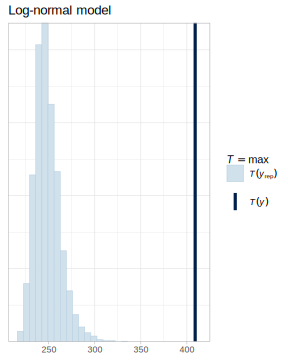
\includegraphics[width=0.45\linewidth]{bookdown_files/figure-latex/ppcheckmax-2} \caption{Distribution of maximum values in a posterior predictive check. The maximum in the data is 409 ms.}\label{fig:ppcheckmax}
\end{figure}

Figure \ref{fig:ppcheckmin} shows that the log-normal likelihood does a
slightly better job since the minimum value is contained in the bulk of
the log-normal distribution and in the tail of the normal one. Figure
\ref{fig:ppcheckmax} shows that both models are unable to capture the
maximum value of the observed data. One explanation for this is that the
log-normal-ish observations in our data are being generated by the task
of pressing as fast as possible, while the observations with long
reaction times are being generated by lapses of attention. This would
mean that two probability distributions are mixed here; modeling this
process involves more complex tools that we will treat in chapter
\ref{ch:mixture}.

\section{Summary}\label{summary}

In this chapter, we learned how to fit and interpret a Bayesian model
with a normal likelihood. We looked at the effect of priors by means of
prior predictive distributions and sensitivity analysis. We also looked
at the fit of the posterior, by inspecting the posterior predictive
distribution (descriptive adequacy). Furthermore, we learned how to fit
a Bayesian model with a log-normal likelihood, and how to compare the
predictive accuracy of different models.

\section{Further reading}\label{further-reading-2}

On the topic of priors:

\begin{itemize}
\tightlist
\item
  Chapter 5 of Lunn D, Jackson C, Spiegelhalter DJ, Best N, Thomas A
  (2012)., \emph{The BUGS book: A practical introduction to Bayesian,
  analysis}, volume 98. CRC Press.
\item
  Gelman A, Simpson D, Betancourt M (2017). ``The prior can often, only
  be understood in the context of the likelihood.'', \emph{Entropy},
  \emph{19}(10), 555. doi: 10.3390/e19100555 (URL:,
  \url{https://doi.org/10.3390/e19100555}), .
\item
  Simpson D, Rue H, Riebler A, Martins TG, Sørbye SH (2017).,
  ``Penalising Model Component Complexity: A Principled,, Practical
  Approach to Constructing Priors.'' \emph{Statistical, Science},
  \emph{32}(1), 1-28. ISSN 0883-4237, 2168-8745, doi:, 10.1214/16-STS576
  (URL: \url{https://doi.org/10.1214/16-STS576}),, \textless{}URL:
  \url{https://projecteuclid.org/euclid.ss/1491465621}\textgreater{}.
\item
  Prior distributions for \texttt{rstanarm} models in
  \url{https://mc-stan.org/rstanarm/articles/priors.html}
\item
  Prior choice recommendations in
  \url{https://github.com/stan-dev/stan/wiki/Prior-Choice-Recommendations}
\end{itemize}

\section{Exercises}\label{ex:compbda}

\begin{exercise}
\protect\hypertarget{exr:linearmod}{}{\label{exr:linearmod} }A simple linear
model. \end{exercise}

\vspace{-.5cm}

\begin{enumerate}
\def\labelenumi{\alph{enumi}.}
\tightlist
\item
  Fit the model \texttt{fit\_press} with just a few iterations, say 50
  iterations. What happens?
\item
  Using uniform distributions, choose priors that represent better
  \textbf{your} assumptions about reaction times. What happens with the
  new model?
\end{enumerate}

\begin{exercise}
\protect\hypertarget{exr:compbda-biasedpost}{}{\label{exr:compbda-biasedpost}
}Revisiting the button-pressing example with different priors.
\end{exercise}

\vspace{-.5cm} Can you come up with very informative priors that biases
the posterior in a noticeable way (use normal distributions for priors,
not uniform priors)? Generate and plot prior predictive distributions
based on this prior.

\begin{exercise} \protect\hypertarget{exr:ppd}{}{\label{exr:ppd}
}Posterior predictive distribution and log-normal model.
\end{exercise}

\vspace{-.5cm}

\begin{enumerate}
\def\labelenumi{\alph{enumi}.}
\tightlist
\item
  Generate posterior predictive distributions based on the previous
  model (\ref{ex:compbda-biasedpost}) and plot them.
\item
  For the log-normal model \texttt{fit\_press\_ln}, change the prior of
  \(\sigma\) so that it is a log-normal distribution with location
  (\(\mu\)) of \(-2\) and scale (\(\sigma\)) of \(.5\). What does such a
  prior imply about your belief regarding button-pressing times in
  milliseconds? Is it a good prior? Generate and plot prior predictive
  distributions. Do the new estimates change compared to earlier models
  when you fit the model?
\item
  For the log-normal model, what is the mean (rather than median) time
  that takes to press the space bar, what is the standard deviation of
  the reaction times in milliseconds?
\end{enumerate}

\begin{exercise} \protect\hypertarget{exr:skew}{}{\label{exr:skew}
}A skew normal distribution. \end{exercise}

Would it make sense to use a ``skew normal distribution'' instead of the
lognormal? The skew normal distribution has three parameters location
\(\xi\), scale \(\omega\), and shape \(\alpha\). The distribution is
right skewed if \(\alpha >0\), is left skewed if \(\alpha <0\), and is
identical to the regular normal distribution if \(\alpha =0\). For
fitting this in \texttt{brms}, one needs to change \texttt{family} and
set it to \texttt{skew\_normal()}, and add a prior of
\texttt{class\ =\ alpha} (location remains \texttt{class\ =\ Intercept}
and scale, \texttt{class\ =\ sigma}).

\begin{enumerate}
\def\labelenumi{\alph{enumi}.}
\tightlist
\item
  Fit this model with a prior that assigns approximately 95\% of the
  prior probability mass of \texttt{alpha} to be between 0 and 10.
\item
  Generate posterior predictive distributions and compare the posterior
  distribution of summary statistics of the skew normal with the normal
  and log-normal
\end{enumerate}

\section{Appendix}\label{appendix}

\subsection{\texorpdfstring{Generating prior predictive distributions
with
\texttt{brms}}{Generating prior predictive distributions with brms}}\label{app:pp}

\texttt{brms} can generate prior predictive distributions for us
ignoring the data, by using \texttt{sample\_prior\ =\ "only"}. Since we
are not fitting any model, we can ignore the messages and warnings, and
we set only one chain with 1000 iterations and no warmup.
\texttt{posterior\_predict(...)} and
\texttt{predict(...,\ summary\ =\ FALSE)} will return an array of
\(N_{samples}\) by \(N_{observations}\) of prior predictions (this is
because of \texttt{sample\_prior\ =\ "only"}), and we'll need to
manipulate the array to get the desired data frame.

\begin{Shaded}
\begin{Highlighting}[]
\NormalTok{fit_press_prior <-}\StringTok{ }\KeywordTok{brm}\NormalTok{(rt }\OperatorTok{~}\StringTok{ }\DecValTok{1}\NormalTok{,}
  \DataTypeTok{family =} \KeywordTok{gaussian}\NormalTok{(),}
  \DataTypeTok{prior =} \KeywordTok{c}\NormalTok{(}
    \KeywordTok{prior}\NormalTok{(}\KeywordTok{uniform}\NormalTok{(}\DecValTok{0}\NormalTok{, }\DecValTok{60000}\NormalTok{), }\DataTypeTok{class =}\NormalTok{ Intercept),}
    \KeywordTok{prior}\NormalTok{(}\KeywordTok{uniform}\NormalTok{(}\DecValTok{0}\NormalTok{, }\DecValTok{2000}\NormalTok{), }\DataTypeTok{class =}\NormalTok{ sigma)}
\NormalTok{  ),}
  \DataTypeTok{sample_prior =} \StringTok{"only"}\NormalTok{,}
  \DataTypeTok{warmup =} \DecValTok{0}\NormalTok{,}
  \DataTypeTok{chains =} \DecValTok{1}\NormalTok{,}
  \DataTypeTok{iter =} \DecValTok{1000}\NormalTok{,}
  \DataTypeTok{data =}\NormalTok{ df_noreading_data}
\NormalTok{)}

\CommentTok{# predict with summary = FALSE returns a N_samples * N_obs array:}
\NormalTok{prior_pred <-}\StringTok{ }\KeywordTok{predict}\NormalTok{(fit_press_prior, }\DataTypeTok{summary =} \OtherTok{FALSE}\NormalTok{) }\OperatorTok
\StringTok{  }\CommentTok{# array_banch converts it in a list of N_samples elements,}
\StringTok{  }\CommentTok{# and in each element a dataset of N_obs:}
\StringTok{  }\KeywordTok{array_branch}\NormalTok{(}\DecValTok{1}\NormalTok{) }\OperatorTok
\StringTok{  }\CommentTok{# map_dfr loops over the N_sample elements of the list and builds a data frame}
\StringTok{  }\KeywordTok{map_dfr}\NormalTok{(}\OperatorTok{~}\StringTok{ }\KeywordTok{tibble}\NormalTok{(}\DataTypeTok{rt_pred =}\NormalTok{ .x, }\DataTypeTok{trialn =} \KeywordTok{seq_along}\NormalTok{(.x)), }\DataTypeTok{.id =} \StringTok{"sample_n"}\NormalTok{) }\OperatorTok
\StringTok{  }\CommentTok{# .id is always a string and needs to be converted}
\StringTok{  }\KeywordTok{mutate}\NormalTok{(}\DataTypeTok{sample_n =} \KeywordTok{as.numeric}\NormalTok{(sample_n))}
\end{Highlighting}
\end{Shaded}

\chapter{Bayesian regression models}\label{ch:reg}

We generally run experiments because we are interested in the
relationship between two or more observables. A regression will tell us
how our \emph{dependent variable}, also called the \emph{response} or
\emph{outcome variable} (e.g., pupil size, reaction times, accuracy,
etc) is affected by one or many \emph{independent variables},
\emph{predictors}, or \emph{explanatory variables}. Predictors can be
categorical (e.g., male or female), ordinal (first, second, third, etc),
or continuous. We will assume that our predictors are continuous in this
chapter, and we will refer to them (mostly) as \emph{covariates}.
Unfortunately, many times it will happen that the same concept has
different names, and a name can be associated with different concepts
(mostly depending on the context). \emph{Covariates} are sometimes used
to refer to control variables; we won't use them with this meaning in
the book, but it's a good idea to bear this in mind.

\begin{rmdnote} to-do: This could be expanded much more.
\end{rmdnote}

\section{A first linear regression: Does attentional load affect pupil
size?}\label{sec:pupil}

We'll look at the effect of cognitive processing on human pupil size to
illustrate the use of Bayesian linear regression models. Although pupil
size is mostly related to the amount of light that reaches the retina or
the distance to a perceived object, pupil sizes are also systematically
influenced by cognitive processing: It has been found that increased
cognitive load leads to an increase in the pupil size \citep[for a
review, see][]{mathotPupillometryPsychologyPhysiology2018}.

For this example, we'll use the data of one participant's pupil size of
the control experiment of \citet{wahnPupilSizesScale2016} averaged by
trial.\footnote{The full dataset can be found in
  \url{https://osf.io/z43dz/}. We show our preprocessing in the appendix
  of this chapter, section \ref{sec:preprocessingpupil}.} In this
experiment, a participant covertly tracked between zero and five objects
among several randomly moving objects on a computer screen. This task is
called multiple object tracking \citep[or
MOT:][]{pylyshynTrackingMultipleIndependent1988} task. First, several
objects appear on the screen, and a subset of them are indicated as
``targets'' at the beginning. Then, the objects start moving randomly
across the screen and become indistinguishable. After several seconds,
the objects stop moving and the participant need to indicate which
objects were the targets. See also Figure \ref{fig:mot}. Our research
goal is to examine how the number of moving objects being tracked, that
is how the attentional load, affects pupil size.




\begin{figure}

{\centering 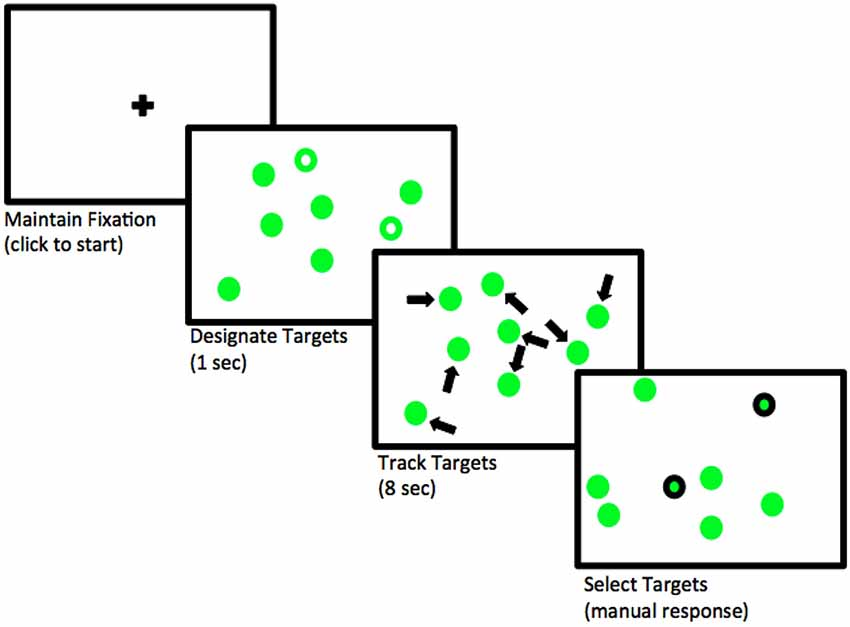
\includegraphics[width=0.8\linewidth]{cc_figure/MOT} 

}

\caption{Flow of events in a trial where two objects need to be
tracked. Adapted from \citet{Blumberg2015}; licensed under CC BY 4.0.}\label{fig:mot}
\end{figure}

\subsection{Likelihood and priors}\label{likelihood-and-priors}

We will model pupil size as normally distributed, because we are not
expecting a skew, and we have no further information available about the
distribution of pupil sizes. (Notice that pupil sizes cannot be of size
zero or negative, so we know for sure that this choice is not exactly
right.) For simplicity, we are also going to assume a linear
relationship between load and the pupil size.

Let's summarize our assumptions:

\begin{enumerate}
\def\labelenumi{\arabic{enumi}.}
\tightlist
\item
  There is some average pupil size represented by \(\alpha\).
\item
  The increase of attentional load has a linear relationship with pupil
  size, determined by \(\beta\).
\item
  There is some noise in this process, that is, variability around the
  true pupil size i.e., a scale, \(\sigma\).
\item
  The noise is normally distributed.
\end{enumerate}

Our likelihood will be as follows:

\begin{equation}
p\_size_n \sim Normal(\alpha + c\_load_n \cdot \beta,\sigma)
\end{equation}

where \(n\) indicates the observation number with \(n = 1 \ldots N\)

This means that the formula that we'll use in \texttt{brms} will be
\texttt{p\_size\ \textasciitilde{}\ 1\ +\ c\_load}, where \texttt{1}
represents the intercept, \(\alpha\), which doesn't depend on a
covariate or predictor, and \texttt{c\_load} is our covariate that is
multiplied by \(\beta\). We will generally indicate with the prefix
\texttt{c\_}, that a covariate (in this case load) is centered (i.e., we
subtract from each value the mean of all values). If load is centered,
the intercept represents the pupil size at the average load in the
experiment (because at the average load, the centered load is zero, and
then \(\alpha + 0 \cdot \beta\)). Alternatively, if the load would not
have been centered (i.e., starts with no load, then one, two, etc), then
the intercept would represent the pupil size when there is no load.
Although this formula would be enough to fit a frequentist model with
\texttt{lm(p\_size\ \textasciitilde{}\ 1\ +\ c\_load,\ dataset)}, when
we fit a Bayesian model, we have to specify priors for each of the
parameters.

For setting the priors, we need information about pupil sizes. While we
might know that pupil diameters range between 2 to 4 mm in bright light
to 4 to 8 mm in the dark \citep{spectorPupils1990}, this experiment was
conducted with the Eyelink-II eyetracker which measures the pupils in
arbitrary units \citep{hayesMappingCorrectingInfluence2016}. If this is
our first analysis of pupil size, before setting up the priors, we'll
need to look at some measures of pupil size. (If we had analyzed this
type of data before, we could also look at estimates from previous
experiments). Fortunately, we have some measurements of the same
participant with no attentional load for the first 100ms, each 10 ms, in
\texttt{pupil\_pilot.csv}: This will give us some idea about the order
of magnitude of our dependent variable.

\begin{Shaded}
\begin{Highlighting}[]
\NormalTok{df_pupil_pilot <-}\StringTok{ }\KeywordTok{read_csv}\NormalTok{(}\StringTok{"./data/pupil_pilot.csv"}\NormalTok{)}
\NormalTok{df_pupil_pilot}\OperatorTok{$}\NormalTok{p_size }\OperatorTok\StringTok{ }\KeywordTok{summary}\NormalTok{()}
\end{Highlighting}
\end{Shaded}

\begin{verbatim}
##    Min. 1st Qu.  Median    Mean 3rd Qu.    Max. 
##     852     856     862     861     866     868
\end{verbatim}

With this information we can set a regularizing prior for \(\alpha\). We
center the prior around 1000 to be in the right order of
magnitude.\footnote{The average pupil size will probably be higher than
  800, since this measurement was with no load, but, in any case, the
  exact number won't matter, any mean between 500-1500 would be fine if
  the standard deviation is large.} Since we don't know how much pupil
sizes are going to vary by load yet, we include a rather wide prior by
defining it as a normal distribution and setting its standard deviation
as \(500\).

\begin{equation}
\alpha \sim Normal(1000, 500) 
\end{equation}

Given that our covariate load is centered, with the prior for
\(\alpha\), we are saying that we suspect that the average pupil size
for the average load in the experiment will be in a 95\% central
interval limited by approximately \(1000 \pm 2 \cdot 500 = [0, 2000]\)
units. We can caclulate this with more precision in \texttt{R} using the
\texttt{qnorm} function:

\begin{Shaded}
\begin{Highlighting}[]
\KeywordTok{qnorm}\NormalTok{(}\KeywordTok{c}\NormalTok{(.}\DecValTok{025}\NormalTok{, }\FloatTok{.975}\NormalTok{), }\DataTypeTok{mean =} \DecValTok{1000}\NormalTok{, }\DataTypeTok{sd =} \DecValTok{500}\NormalTok{)}
\end{Highlighting}
\end{Shaded}

\begin{verbatim}
## [1]   20 1980
\end{verbatim}

We know that the measurements of the pilot data are strongly correlated
because they were taken together just some milliseconds apart. For this
reason, they won't tell us how much the pupil size can vary. We set up a
quite weak prior for \(\sigma\) that encodes our lack of precise
information: \(\sigma\) is surely larger than zero and has to be in the
order of magnitude of the pupil size with no load.

\begin{equation}
\sigma \sim Normal_+(0, 1000)
\end{equation}

With this prior for \(\sigma\), we are saying that we expect that the
standard deviation of the pupil sizes should be in the following 95\%
central interval. (Notice that we use \texttt{qtnorm(...,\ a\ =\ 0)} and
not \texttt{qnorm()}).

\begin{Shaded}
\begin{Highlighting}[]
\KeywordTok{c}\NormalTok{(}\KeywordTok{qtnorm}\NormalTok{(.}\DecValTok{025}\NormalTok{, }\DataTypeTok{mean =} \DecValTok{0}\NormalTok{, }\DataTypeTok{sd =} \DecValTok{1000}\NormalTok{, }\DataTypeTok{a =} \DecValTok{0}\NormalTok{),}
  \KeywordTok{qtnorm}\NormalTok{(.}\DecValTok{975}\NormalTok{, }\DataTypeTok{mean =} \DecValTok{0}\NormalTok{, }\DataTypeTok{sd =} \DecValTok{1000}\NormalTok{, }\DataTypeTok{a =} \DecValTok{0}\NormalTok{))}
\end{Highlighting}
\end{Shaded}

\begin{verbatim}
## [1]   31.3 2241.4
\end{verbatim}

Notice that the mean of \(Normal_+\), a normal distribution truncated in
zero allowing for only positive values, does not coincide with its
location indicated with the parameter \(\mu\) (and neither the standard
deviation coincides with the scale, \(\sigma\)); see also Box
\ref{thm:truncation}.

\begin{Shaded}
\begin{Highlighting}[]
\NormalTok{samples <-}\StringTok{ }\KeywordTok{rtnorm}\NormalTok{(}\DecValTok{20000}\NormalTok{, }\DataTypeTok{mean =} \DecValTok{0}\NormalTok{, }\DataTypeTok{sd =} \DecValTok{1000}\NormalTok{, }\DataTypeTok{a =} \DecValTok{0}\NormalTok{)}
\KeywordTok{mean}\NormalTok{(samples)}
\end{Highlighting}
\end{Shaded}

\begin{verbatim}
## [1] 794
\end{verbatim}

We still need to set a prior for \(\beta\), the change in pupil size
produced by the attentional load. Given that pupil size changes are not
easily perceptible (we don't see them in our day-to-day life), we expect
them to be much smaller than the pupil size, so we use the following
prior:

\begin{equation}
\beta \sim Normal(0, 100)
\end{equation}

With the prior of \(\beta\), we are saying that we don't really know if
the attentional load will increase or even decrease the pupil size
(notice that is centered in zero), but we do know that one unit of load
(that is one more object to track) will potentially change the pupil
size in a way that is consistent with the following 95\% central
interval.

\begin{Shaded}
\begin{Highlighting}[]
\KeywordTok{c}\NormalTok{(}\KeywordTok{qnorm}\NormalTok{(.}\DecValTok{025}\NormalTok{, }\DataTypeTok{mean =} \DecValTok{0}\NormalTok{, }\DataTypeTok{sd =} \DecValTok{100}\NormalTok{), }\KeywordTok{qnorm}\NormalTok{(.}\DecValTok{975}\NormalTok{, }\DataTypeTok{mean =} \DecValTok{0}\NormalTok{, }\DataTypeTok{sd =} \DecValTok{100}\NormalTok{))}
\end{Highlighting}
\end{Shaded}

\begin{verbatim}
## [1] -196  196
\end{verbatim}

That is, we don't expect changes in size that increase or decrease the
pupil size in more than 200 units.

\Begin{extra}

\begin{theorem}
\protect\hypertarget{thm:truncation}{}{\label{thm:truncation}
}\textbf{Truncated distributions} \end{theorem}

Any distribution can be truncated. For a continuous distribution, the
truncated version of the original distribution will have non zero
probability density values for a continuous subset of the original
coverage. To make it more concrete, in our previous example, the normal
distribution has coverage for values between minus infinity to plus
infinity, and our truncated version \(Normal_+\) has coverage between
zero and plus inifinity: all negative values have a probability density
of zero. Let's see how we can generalize this to be able to understand
any truncation of any continuous distribution. (For the discrete case we
can simply replace the integral for a sum, and PDF for PMF).

From the axiomatic definitions of probability we know that the area
below a PDF, \(f(x)\), must be equal to one (\ref{introprob}). More
formally, this means that the integral of \(f\) evaluated as
\(f(\infty <X < \infty)\) should be equal to one:

\begin{equation}
\int_{-\infty}^{\infty} f(x) dx = 1
\end{equation}

But if the distribution is truncated, \(f\), is going to be evaluated in
some subset of its possible values, \(f(a <X < b)\); in the specific
case of \(Normal_+\), for example, \(a = 0\), and \(b=\infty\). In the
general case, this means that the integral of the PDF evaluated for
\(a <X < b\) can be lower than one.

\begin{equation}
\int_{a}^{b} f(x) dx \leq 1
\end{equation}

We want to ensure that we build a new PDF for the truncated distribution
so that even though it has less coverage than the non-truncated version
still integrates to one. To achieve this, we normalize the PDF with
restricted coverage, by conditioning the PDF to the actual range it has
coverage, that is, by dividing the ``unnormalized'' PDF by the total
area of \(f(a <X < b)\):

\begin{equation}
f_{[a,b]}(x) = \frac{f(x)}{\int_{a}^{b} f(x) dx}
\end{equation}

The denominator of the previous equation is the difference between the
CDF evaluated at \(X = b\) and the CDF evaluated at \(X =a\); this can
be written as \(F(b) - F(a)\):

\begin{equation}
f_{[a,b]}(x) = \frac{f(x)}{F(b) - F(a)}
\label{eq:truncPDF}
\end{equation}

For the specific case, where \(f(x)\) is \(Normal(x | 0, \sigma)\) and
we want the PDF of \(Normal_+(x | 0, \sigma)\), and thus \(a= 0\) and
\(b =\infty\).

\begin{equation}
Normal_+(x |0, \sigma) = \frac{Normal(x | 0, \sigma)}{1/2}
\end{equation}

Because \(F(X= b =\infty) = 1\) and \(F(X = a = 0) = 1/2\).

You can verify this in R (and this is valid for any value of
\texttt{sd}).

\begin{Shaded}
\begin{Highlighting}[]
\KeywordTok{dnorm}\NormalTok{(}\DecValTok{1}\NormalTok{,}\DataTypeTok{mean =} \DecValTok{0}\NormalTok{) }\OperatorTok{*}\StringTok{ }\DecValTok{2} \OperatorTok{==}\StringTok{ }\KeywordTok{dtnorm}\NormalTok{(}\DecValTok{1}\NormalTok{, }\DataTypeTok{mean =} \DecValTok{0}\NormalTok{, }\DataTypeTok{a =} \DecValTok{0}\NormalTok{)}
\end{Highlighting}
\end{Shaded}

\begin{verbatim}
## [1] TRUE
\end{verbatim}

Notice that unless the truncation of the normal distribution is
symmetrical, the location, \(\mu\), of the truncated normal does not
coincide with the mean, and for any type of truncation, the scale,
\(\sigma\), does not coincide with the standard deviation. Confusingly
enough, the arguments of the family of functions \texttt{*tnorm} keep
the names of the family of functions \texttt{*norm}, and the location is
called \texttt{mean} and the scale \texttt{sd}.

For example, the mean of the truncated normal with boundaries \(a\) and
\(b\), given its location and scale is as follows:

\begin{equation}
\operatorname {E} (X\mid a<X<b) = \mu +\sigma {\frac {\phi (\alpha )-\phi (\beta )}{\Phi (\beta )-\Phi (\alpha )}} 
\end{equation}

where \(\alpha =(a-\mu )/\sigma\), \(\beta =(b-\mu )/\sigma\),
\(\phi(X)\) is the PDF of the standard normal (\(\mu=0, \sigma=1\))
evaluated at \(X\), and \(\Phi(X)\) is the CDF of the standard normal
evaluated at \(X\).

We build a function in R that calculates the mean for any truncated
normal as follows:

\begin{Shaded}
\begin{Highlighting}[]
\NormalTok{mean_n_ab <-}\StringTok{ }\ControlFlowTok{function}\NormalTok{(}\DataTypeTok{mu =} \DecValTok{0}\NormalTok{, }\DataTypeTok{sigma =} \DecValTok{1}\NormalTok{, }\DataTypeTok{a =} \OperatorTok{-}\OtherTok{Inf}\NormalTok{, }\DataTypeTok{b =} \OtherTok{Inf}\NormalTok{) \{}
\NormalTok{  alpha <-}\StringTok{ }\NormalTok{(a }\OperatorTok{-}\StringTok{ }\NormalTok{mu) }\OperatorTok{/}\StringTok{ }\NormalTok{sigma}
\NormalTok{  beta <-}\StringTok{ }\NormalTok{(b }\OperatorTok{-}\StringTok{ }\NormalTok{mu) }\OperatorTok{/}\StringTok{ }\NormalTok{sigma}
\NormalTok{  mu }\OperatorTok{+}\StringTok{ }\NormalTok{sigma }\OperatorTok{*}\StringTok{ }\NormalTok{(}\KeywordTok{dnorm}\NormalTok{(alpha) }\OperatorTok{-}\StringTok{ }\KeywordTok{dnorm}\NormalTok{(beta))}\OperatorTok{/}
\StringTok{    }\NormalTok{(}\KeywordTok{pnorm}\NormalTok{(beta) }\OperatorTok{-}\StringTok{ }\KeywordTok{pnorm}\NormalTok{(alpha))}
\NormalTok{\}}
\end{Highlighting}
\end{Shaded}

We can try it in R for our \(Normal_+(0, 1000)\):

\begin{Shaded}
\begin{Highlighting}[]
\KeywordTok{mean_n_ab}\NormalTok{(}\DataTypeTok{mu =} \DecValTok{0}\NormalTok{, }\DataTypeTok{sigma =} \DecValTok{1000}\NormalTok{, }\DataTypeTok{a =} \DecValTok{0}\NormalTok{)}
\end{Highlighting}
\end{Shaded}

\begin{verbatim}
## [1] 798
\end{verbatim}

We get similar results calculating the average of 20000 samples.

\begin{Shaded}
\begin{Highlighting}[]
\KeywordTok{mean}\NormalTok{(}\KeywordTok{rtnorm}\NormalTok{(}\DecValTok{20000}\NormalTok{, }\DataTypeTok{mean =} \DecValTok{0}\NormalTok{, }\DataTypeTok{sd =} \DecValTok{1000}\NormalTok{, }\DataTypeTok{a =} \DecValTok{0}\NormalTok{))}
\end{Highlighting}
\end{Shaded}

\begin{verbatim}
## [1] 796
\end{verbatim}

\End{extra}

\subsection{\texorpdfstring{The \texttt{brms}
model}{The brms model}}\label{the-brms-model}

Before fitting the \texttt{brms} model, we load the data and center the
predictor \texttt{load}:

\begin{Shaded}
\begin{Highlighting}[]
\NormalTok{(df_pupil_data <-}\StringTok{ }\KeywordTok{read_csv}\NormalTok{(}\StringTok{"data/pupil.csv"}\NormalTok{) }\OperatorTok
\StringTok{   }\KeywordTok{mutate}\NormalTok{(}\DataTypeTok{c_load =}\NormalTok{ load }\OperatorTok{-}\StringTok{ }\KeywordTok{mean}\NormalTok{(load)))}
\end{Highlighting}
\end{Shaded}

\begin{verbatim}
## # A tibble: 41 x 4
##   trial  load p_size c_load
##   <dbl> <dbl>  <dbl>  <dbl>
## 1     1     2  1021. -0.439
## 2     2     1   951. -1.44 
## 3     3     5  1064.  2.56 
## 4     4     4   913.  1.56 
## 5     5     0   603. -2.44 
## # ... with 36 more rows
\end{verbatim}

Now we can fit the \texttt{brms} model:

\begin{Shaded}
\begin{Highlighting}[]
\NormalTok{fit_pupil <-}\StringTok{ }\KeywordTok{brm}\NormalTok{(p_size }\OperatorTok{~}\StringTok{ }\DecValTok{1} \OperatorTok{+}\StringTok{ }\NormalTok{c_load,}
                 \DataTypeTok{data =}\NormalTok{ df_pupil_data,}
                 \DataTypeTok{family =} \KeywordTok{gaussian}\NormalTok{(),}
                 \DataTypeTok{prior =} \KeywordTok{c}\NormalTok{(}
                     \KeywordTok{prior}\NormalTok{(}\KeywordTok{normal}\NormalTok{(}\DecValTok{1000}\NormalTok{, }\DecValTok{500}\NormalTok{), }\DataTypeTok{class =}\NormalTok{ Intercept),}
                     \KeywordTok{prior}\NormalTok{(}\KeywordTok{normal}\NormalTok{(}\DecValTok{0}\NormalTok{, }\DecValTok{1000}\NormalTok{), }\DataTypeTok{class =}\NormalTok{ sigma),}
                     \KeywordTok{prior}\NormalTok{(}\KeywordTok{normal}\NormalTok{(}\DecValTok{0}\NormalTok{, }\DecValTok{100}\NormalTok{), }\DataTypeTok{class =}\NormalTok{ b, }\DataTypeTok{coef =}\NormalTok{ c_load)}
\NormalTok{                 )) }
\end{Highlighting}
\end{Shaded}

The only difference from our previous models is that we now have a
predictor in the formula and in the priors. Priors for predictors are
indicated with \texttt{class\ =\ b}, and the specific predictor with
\texttt{coef\ =\ c\_load}. If we want to set the same priors to
different predictors we can omit the argument \texttt{coef}. We can
remove the \texttt{1} of the formula, and \texttt{brm()} will fit the
exact same model as when we specify \texttt{1} explicitly. If we really
want to remove the intercept we indicate this with \texttt{0\ +...} or
\texttt{-1\ +...}. See also the Box \ref{thm:intercept} for more details
about the treatment of the intercepts by \texttt{brms}.

We can inspect the output of our model now:

\begin{Shaded}
\begin{Highlighting}[]
\KeywordTok{plot}\NormalTok{(fit_pupil)}
\end{Highlighting}
\end{Shaded}

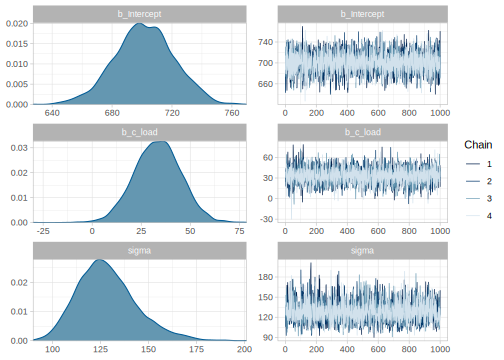
\includegraphics{bookdown_files/figure-latex/unnamed-chunk-98-1.pdf}

\begin{Shaded}
\begin{Highlighting}[]
\NormalTok{fit_pupil}
\end{Highlighting}
\end{Shaded}

\begin{verbatim}
##  Family: gaussian 
##   Links: mu = identity; sigma = identity 
## Formula: p_size ~ 1 + c_load 
##    Data: df_pupil_data (Number of observations: 41) 
## Samples: 4 chains, each with iter = 2000; warmup = 1000; thin = 1;
##          total post-warmup samples = 4000
## 
## Population-Level Effects: 
##           Estimate Est.Error l-95% CI u-95% CI Rhat Bulk_ESS Tail_ESS
## Intercept   701.39     20.29   662.13   741.93 1.00     3682     2696
## c_load       33.54     12.10    10.24    57.61 1.00     3728     2804
## 
## Family Specific Parameters: 
##       Estimate Est.Error l-95% CI u-95% CI Rhat Bulk_ESS Tail_ESS
## sigma   128.39     14.99   103.79   161.41 1.00     3680     2542
## 
## Samples were drawn using sampling(NUTS). For each parameter, Bulk_ESS
## and Tail_ESS are effective sample size measures, and Rhat is the potential
## scale reduction factor on split chains (at convergence, Rhat = 1).
\end{verbatim}

We discuss how we could communicate the relevant information in the next
section.

\Begin{extra}

\begin{theorem}
\protect\hypertarget{thm:intercept}{}{\label{thm:intercept}
}\textbf{Intercepts in \texttt{brms}} \end{theorem}

When we set up a prior for the intercept in \texttt{brms}, we actually
set a prior for an intercept given that all the predictors are centered.
The reason for this is that \texttt{brms} increases sampling efficiency
by \emph{automatically} centering all the predictors (that is the
population-level design matrix X is internally centered around its
column means when \texttt{brms} fits a model). This did not matter in
our previous examples because we centered our predictor (or we had
none), but it might matter if we want to have uncentered predictors. In
the design we are discussing, a non-centered predictor of load will mean
that the intercept, \(\alpha\), has a straightforward interpretation (in
many cases, however, an intercept with a non-centered predictor won't
have a straightforward interpretation): the pupil size when there is no
attention load.

We might be more sure about prior values for the no load condition, and
we want to set the following prior to our new \(\alpha\):
\(Normal(800,200)\). In this case, we should fit the following model:

\begin{Shaded}
\begin{Highlighting}[]
\NormalTok{fit_pupil_non_centered <-}\StringTok{ }\KeywordTok{brm}\NormalTok{(p_size }\OperatorTok{~}\StringTok{ }\DecValTok{0} \OperatorTok{+}\StringTok{ }\NormalTok{Intercept }\OperatorTok{+}\StringTok{ }\NormalTok{load,}
                 \DataTypeTok{data =}\NormalTok{ df_pupil_data,}
                 \DataTypeTok{family =} \KeywordTok{gaussian}\NormalTok{(),}
                 \DataTypeTok{prior =} \KeywordTok{c}\NormalTok{(}
                     \KeywordTok{prior}\NormalTok{(}\KeywordTok{normal}\NormalTok{(}\DecValTok{800}\NormalTok{, }\DecValTok{200}\NormalTok{), }\DataTypeTok{class =}\NormalTok{ b, }\DataTypeTok{coef =}\NormalTok{ Intercept),}
                     \KeywordTok{prior}\NormalTok{(}\KeywordTok{normal}\NormalTok{(}\DecValTok{0}\NormalTok{, }\DecValTok{1000}\NormalTok{), }\DataTypeTok{class =}\NormalTok{ sigma),}
                     \KeywordTok{prior}\NormalTok{(}\KeywordTok{normal}\NormalTok{(}\DecValTok{0}\NormalTok{, }\DecValTok{100}\NormalTok{), }\DataTypeTok{class =}\NormalTok{ b, }\DataTypeTok{coef =}\NormalTok{ load)}
\NormalTok{                 ))}
\end{Highlighting}
\end{Shaded}

Notice that we remove the regular centered intercept by adding
\texttt{0} to the formula, and we replace it with the ``actual''
intercept we want to set priors to with \texttt{Intercept}---this is a
reserved word, and thus we cannot name any predictor with this name.
This new parameter is also of the class \texttt{b}, so its prior needs
to be defined accordingly.

The output below shows that, as expected, while the posterior for the
intercept has changed noticeably, the posterior for the effect of load
remains virtually unchanged.

\begin{Shaded}
\begin{Highlighting}[]
\KeywordTok{posterior_summary}\NormalTok{(fit_pupil_non_centered)}
\end{Highlighting}
\end{Shaded}

\begin{verbatim}
##             Estimate Est.Error    Q2.5  Q97.5
## b_Intercept    623.5     35.63  552.05  692.9
## b_load          32.4     12.07    8.77   56.4
## sigma          129.0     15.56  102.56  163.3
## lp__          -271.1      1.27 -274.39 -269.6
\end{verbatim}

Notice the following potential pitfall. A model like the one below will
fit a non-centered load predictor, but will assign a prior of
\(Normal(800,200)\) to the intercept of a \emph{centered} model,
\(\alpha_{centered}\), and not the current intercept, \(\alpha\).

\begin{Shaded}
\begin{Highlighting}[]
\NormalTok{fit_pupil_wrong <-}\StringTok{ }\KeywordTok{brm}\NormalTok{(p_size }\OperatorTok{~}\StringTok{ }\DecValTok{1} \OperatorTok{+}\StringTok{ }\NormalTok{load,}
                 \DataTypeTok{data =}\NormalTok{ df_pupil_data,}
                 \DataTypeTok{family =} \KeywordTok{gaussian}\NormalTok{(),}
                 \DataTypeTok{prior =} \KeywordTok{c}\NormalTok{(}
                     \KeywordTok{prior}\NormalTok{(}\KeywordTok{normal}\NormalTok{(}\DecValTok{800}\NormalTok{, }\DecValTok{100}\NormalTok{), }\DataTypeTok{class =}\NormalTok{ Intercept),}
                     \KeywordTok{prior}\NormalTok{(}\KeywordTok{normal}\NormalTok{(}\DecValTok{0}\NormalTok{, }\DecValTok{1000}\NormalTok{), }\DataTypeTok{class =}\NormalTok{ sigma),}
                     \KeywordTok{prior}\NormalTok{(}\KeywordTok{normal}\NormalTok{(}\DecValTok{0}\NormalTok{, }\DecValTok{100}\NormalTok{), }\DataTypeTok{class =}\NormalTok{ b, }\DataTypeTok{coef =}\NormalTok{ load)}
\NormalTok{                 ))}
\end{Highlighting}
\end{Shaded}

What does it mean to set a prior to \(\alpha_{centered}\) in a model
that \emph{doesn't} include \(\alpha_{centered}\)?

Notice that the fitted values of the non-centered model and the centered
one are identical, that is, the expected values of the response
distribution without the residual error (when \(\sigma =0\)) are
identical for both models:

\begin{equation}
\alpha + load_n \cdot \beta = \alpha_{centered} + (load_n - mean(load)) \cdot \beta 
\label{eq:fitted}
\end{equation}

The left side of Equation \eqref{eq:fitted} refers to the fitted values
based on our current non-centered model, and the right side refers to
the fitted values based on the centered model. We can re-arrange terms
to understand what is the effect of a prior on \(\alpha_{centered}\) in
our model that \emph{doesn't} include \(\alpha_{centered}\).

\begin{equation}
\begin{aligned}
\alpha + load_n \cdot \beta &= \alpha_{centered} + load_n\cdot \beta - mean(load) \cdot \beta\\
\alpha  &= \alpha_{centered}  - mean(load) \cdot \beta\\
\alpha + mean(load) \cdot \beta  &= \alpha_{centered}  
\end{aligned}
\end{equation}

That means that we are actually setting our prior to
\(\alpha + mean(load) \cdot \beta\). When \(\beta\) is very small, and
the prior for \(\alpha\) is very wide, we might hardly notice the
difference between setting a prior to \(\alpha_{centered}\) or to our
actual \(\alpha\) in a non-centered model (especially if the likelihood
dominates anyway). But it's a good idea to pay attention to what are the
parameters we are setting priors to.

\End{extra}

\subsection{How to communicate the
results?}\label{how-to-communicate-the-results}

We want to answer our research question ``What is the effect of
attentional load on the participant's pupil size?'' For that we'll need
to examine what happens with \(\beta\), which is \texttt{c\_load} in the
summary of \texttt{brms}. The summary of the posterior tells us that the
most likely values of \(\beta\) will be around the mean of the
posterior, 33.54, and we can be 95\% certain that the true value of
\(\beta\) \emph{given the model and the data} lies between 10.24 and
57.61.

We see that as the attentional load increases, the pupil size of the
participant becomes larger. If we want to determine how likely it is
that the pupil size increased rather than decreased, we can examine the
proportion of samples above zero. (Notice that the intercept and the
slopes, are always preceded by \texttt{b\_} in \texttt{brms}. One can
see all the names of parameters being estimated with
\texttt{parnames()}.)

\begin{Shaded}
\begin{Highlighting}[]
\KeywordTok{mean}\NormalTok{(}\KeywordTok{posterior_samples}\NormalTok{(fit_pupil)}\OperatorTok{$}\NormalTok{b_c_load }\OperatorTok{>}\StringTok{ }\DecValTok{0}\NormalTok{)}
\end{Highlighting}
\end{Shaded}

\begin{verbatim}
## [1] 0.996
\end{verbatim}

\textbf{Take into account that this probability ignores the possibility
of the participant not being affected at all by the manipulation, this
is because \(P(\beta=0)=0\), we'll come back to this issue in the model
comparison chapter \ref{ch:comparison}.}

\subsection{Descriptive adequacy}\label{sec:pupiladq}

Our model converged and we obtained a posterior distribution. There is,
however, no guarantee that our model was adequate to represent our data.
We can use posterior predictive checks to verify this.

Sometimes it's useful to build our own posterior predictive check to
visualize the fit of our model, as opposed to use the \texttt{pp\_check}
functions as we did before in section \ref{sec:ppd}. For example, here
we use \texttt{posterior\_predict()} to generate 1000 posterior
predictive distributions, and we convert them from an array to a long
data frame.

\begin{Shaded}
\begin{Highlighting}[]
\CommentTok{# we start from an array of 1000 samples by 41 observations}
\NormalTok{df_pupil_pred <-}\StringTok{ }\KeywordTok{posterior_predict}\NormalTok{(fit_pupil, }\DataTypeTok{nsamples =} \DecValTok{1000}\NormalTok{) }\OperatorTok
\StringTok{    }\CommentTok{# we convert it to a list of length 1000, with 41 observations in each element:}
\StringTok{    }\KeywordTok{array_branch}\NormalTok{(}\DataTypeTok{margin =} \DecValTok{1}\NormalTok{) }\OperatorTok
\StringTok{    }\CommentTok{# We iterate over the elements (the predicted distributions)}
\StringTok{    }\CommentTok{# and we convert them into a long data frame similar to the data,}
\StringTok{    }\CommentTok{# but with an extra column `iter` indicating from which iteration}
\StringTok{    }\CommentTok{# the sample is coming from.}
\StringTok{    }\KeywordTok{map_dfr}\NormalTok{( }\ControlFlowTok{function}\NormalTok{(yrep_iter) \{}
\NormalTok{        df_pupil_data }\OperatorTok
\StringTok{            }\KeywordTok{mutate}\NormalTok{(}\DataTypeTok{p_size =}\NormalTok{ yrep_iter)}
\NormalTok{    \}, }\DataTypeTok{.id =} \StringTok{"iter"}\NormalTok{) }\OperatorTok
\StringTok{    }\KeywordTok{mutate}\NormalTok{(}\DataTypeTok{iter =} \KeywordTok{as.numeric}\NormalTok{(iter))}
\end{Highlighting}
\end{Shaded}

Then we plot 100 of the densities of the predicted distributions in
blue, and the distribution of our data in black for the five levels of
load in Figure \ref{fig:postpreddens}. We don't have enough data to
derive a strong conclusion: Notice that both the predictive
distributions and our data look very wide, and it hard to tell if the
distribution of the observations could have been generated by our model.
For now we can say that it doesn't look too bad.






\begin{Shaded}
\begin{Highlighting}[]
\NormalTok{df_pupil_pred }\OperatorTok\StringTok{ }\KeywordTok{filter}\NormalTok{(iter }\OperatorTok{<}\StringTok{ }\DecValTok{100}\NormalTok{) }\OperatorTok
\StringTok{    }\KeywordTok{ggplot}\NormalTok{(}\KeywordTok{aes}\NormalTok{(p_size, }\DataTypeTok{group=}\NormalTok{iter)) }\OperatorTok{+}
\StringTok{    }\KeywordTok{geom_line}\NormalTok{(}\DataTypeTok{alpha =} \FloatTok{.05}\NormalTok{, }\DataTypeTok{stat=}\StringTok{"density"}\NormalTok{, }\DataTypeTok{color =} \StringTok{"blue"}\NormalTok{) }\OperatorTok{+}
\StringTok{    }\KeywordTok{geom_density}\NormalTok{(}\DataTypeTok{data=}\NormalTok{df_pupil_data, }\KeywordTok{aes}\NormalTok{(p_size),}
                 \DataTypeTok{inherit.aes =} \OtherTok{FALSE}\NormalTok{, }\DataTypeTok{size =}\DecValTok{1}\NormalTok{)}\OperatorTok{+}
\StringTok{    }\KeywordTok{geom_point}\NormalTok{(}\DataTypeTok{data=}\NormalTok{df_pupil_data, }\KeywordTok{aes}\NormalTok{(}\DataTypeTok{x=}\NormalTok{p_size, }\DataTypeTok{y =} \FloatTok{-0.001}\NormalTok{), }\DataTypeTok{alpha =}\NormalTok{.}\DecValTok{5}\NormalTok{,}
               \DataTypeTok{inherit.aes =} \OtherTok{FALSE}\NormalTok{)}\OperatorTok{+}
\StringTok{    }\KeywordTok{coord_cartesian}\NormalTok{(}\DataTypeTok{ylim=}\KeywordTok{c}\NormalTok{(}\OperatorTok{-}\FloatTok{0.002}\NormalTok{, }\FloatTok{.01}\NormalTok{))}\OperatorTok{+}
\StringTok{    }\KeywordTok{facet_grid}\NormalTok{(load }\OperatorTok{~}\StringTok{ }\NormalTok{.) }
\end{Highlighting}
\end{Shaded}

\begin{figure}
\centering
\includegraphics{bookdown_files/figure-latex/postpreddens-1.pdf}
\caption{\label{fig:postpreddens}The plot shows 100 predicted distributions in blue
density plots, the distribution of pupil size data in black density
plots, and the observed pupil sizes in black dots for the five levels of
attentional load.}
\end{figure}

We can instead look at the distribution of a statistic, such as mean
pupil size by load:

\begin{Shaded}
\begin{Highlighting}[]
\CommentTok{# predicted means:}
\NormalTok{df_pupil_pred_summary <-}\StringTok{ }\NormalTok{df_pupil_pred }\OperatorTok
\StringTok{    }\KeywordTok{group_by}\NormalTok{(iter, load) }\OperatorTok
\StringTok{    }\KeywordTok{summarize}\NormalTok{(}\DataTypeTok{av_p_size =} \KeywordTok{mean}\NormalTok{(p_size))}
\CommentTok{# observed means:}
\NormalTok{df_pupil_summary <-}\StringTok{ }\NormalTok{df_pupil_data }\OperatorTok
\StringTok{    }\KeywordTok{group_by}\NormalTok{(load) }\OperatorTok
\StringTok{    }\KeywordTok{summarize}\NormalTok{(}\DataTypeTok{av_p_size =} \KeywordTok{mean}\NormalTok{(p_size))}
\end{Highlighting}
\end{Shaded}




\begin{Shaded}
\begin{Highlighting}[]
\KeywordTok{ggplot}\NormalTok{(df_pupil_pred_summary, }\KeywordTok{aes}\NormalTok{(av_p_size)) }\OperatorTok{+}
\StringTok{    }\KeywordTok{geom_histogram}\NormalTok{(}\DataTypeTok{alpha=}\NormalTok{.}\DecValTok{5}\NormalTok{)}\OperatorTok{+}
\StringTok{    }\KeywordTok{geom_vline}\NormalTok{(}\KeywordTok{aes}\NormalTok{(}\DataTypeTok{xintercept=}\NormalTok{ av_p_size),}\DataTypeTok{data=}\NormalTok{ df_pupil_summary)}\OperatorTok{+}
\StringTok{    }\KeywordTok{facet_grid}\NormalTok{(load }\OperatorTok{~}\StringTok{ }\NormalTok{.)}
\end{Highlighting}
\end{Shaded}

\begin{figure}
\centering
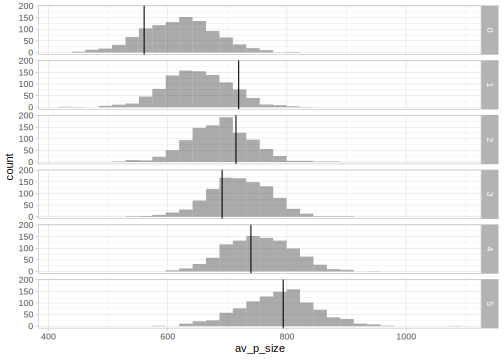
\includegraphics{bookdown_files/figure-latex/postpredmean-1.pdf}
\caption{\label{fig:postpredmean}Distribution of posterior predicted means in gray and
observed pupil size means in black lines by load.}
\end{figure}

Figure \ref{fig:postpredmean} shows that the observed means for no load
and for a load of one are falling in the tails of the distributions.
While our model predicts a monotonic increase of pupil size, the data
might be indicating that the relevant difference is between (i) no load,
(ii) a load between two and three, and then (iii) a load of four, and
(iv) of five. However, given the uncertainty in the posterior predictive
distributions and that the observed means are contained somewhere in the
predicted distributions, it could be the case that with this we are
overinterpreting noise.

\section{Log-normal model: Does trial affect reaction
times?}\label{sec:trial}

Let us revisit the small experiment from section \ref{sec:simplenormal},
where a participant repeatedly pressed the space bar as fast as
possible, without paying attention to the stimuli. We want to know
whether the participant tended to speedup (practice effect) or slowdown
(fatigue effect) while pressing the space bar.

\subsection{Likelihood and priors for the log-normal
model}\label{likelihood-and-priors-for-the-log-normal-model}

If we assume that reaction times are log-normally distributed, we could
fit a likelihood such as the following:

\begin{equation}
rt_n \sim LogNormal(\alpha + c\_trial_n \cdot \beta,\sigma)
\label{eq:rtloglik}
\end{equation}

where \(n =1, \ldots, N\), and \(rt\) is the dependent variable
(reaction times in milliseconds). The variable \(N\) represents the
total number of data points.

We use the same priors as in section \ref{sec:lognormal} for \(\alpha\)
(which is equivalent to \(\mu\) in the previous model) and for
\(\sigma\).

\begin{equation}
\begin{aligned}
\alpha &\sim Normal(6, 1.5) \\
\sigma &\sim Normal_+(0, 1)\\
\end{aligned}
\end{equation}

We still need a prior for \(\beta\). Notice that effects are
multiplicative rather than additive when we assume a log-normal
likelihood and that means that we need to take into account \(\alpha\)
in order to interpret \(\beta\); for more details, see Box
\ref{thm:lognormal}. We are going to try to understand how all our
priors interact together generating some prior predictive distributions.
We start with the following prior centered in zero, a prior agnostic
regarding the direction of the effect, which allows for both a slowdowns
(\(\beta>0\)) or a speedups (\(\beta<0\)):

\begin{equation}
\beta \sim Normal(0, 1)
\end{equation}

We can edit our \texttt{normal\_predictive\_distribution\_fast} from
section \ref{sec:ppd} and make it log-normal and dependent on trial:

\begin{Shaded}
\begin{Highlighting}[]
\NormalTok{lognormal_model_pred <-}\StringTok{ }\ControlFlowTok{function}\NormalTok{(alpha_samples,}
\NormalTok{                                 beta_samples,}
\NormalTok{                                 sigma_samples,}
\NormalTok{                                 N_obs) \{}
    \CommentTok{# pmap extends map2 (and map) for a list of lists:}
    \KeywordTok{pmap_dfr}\NormalTok{(}\KeywordTok{list}\NormalTok{(alpha_samples, beta_samples, sigma_samples),}
             \ControlFlowTok{function}\NormalTok{(alpha, beta, sigma) \{}
                 \KeywordTok{tibble}\NormalTok{(}
                     \DataTypeTok{trialn =} \KeywordTok{seq_len}\NormalTok{(N_obs),}
                     \CommentTok{# we center trial:}
                     \DataTypeTok{c_trial =}\NormalTok{ trialn }\OperatorTok{-}\StringTok{ }\KeywordTok{mean}\NormalTok{(trialn),}
                     \CommentTok{# we change the likelihood: }
                     \CommentTok{# Notice rlnorm and the use of alpha and beta}
                     \DataTypeTok{rt_pred =} \KeywordTok{rlnorm}\NormalTok{(N_obs, alpha }\OperatorTok{+}\StringTok{ }\NormalTok{c_trial }\OperatorTok{*}\StringTok{ }\NormalTok{beta, sigma)}
\NormalTok{                 )}
\NormalTok{             \}, }\DataTypeTok{.id =} \StringTok{"iter"}\NormalTok{) }\OperatorTok
\StringTok{    }\CommentTok{# .id is always a string and needs to be converted to a number}
\StringTok{        }\KeywordTok{mutate}\NormalTok{(}\DataTypeTok{iter =} \KeywordTok{as.numeric}\NormalTok{(iter))}
\NormalTok{\}}
\end{Highlighting}
\end{Shaded}

This is our first attempt for a prior predictive distribution:

\begin{Shaded}
\begin{Highlighting}[]
\NormalTok{N_obs =}\StringTok{ }\DecValTok{361}
\NormalTok{alpha_samples <-}\StringTok{ }\KeywordTok{rnorm}\NormalTok{(}\DecValTok{1000}\NormalTok{, }\DataTypeTok{mean =} \DecValTok{6}\NormalTok{, }\DataTypeTok{sd =}\FloatTok{1.5}\NormalTok{)}
\NormalTok{sigma_samples <-}\StringTok{ }\KeywordTok{rtnorm}\NormalTok{(}\DecValTok{1000}\NormalTok{, }\DataTypeTok{mean =} \DecValTok{0}\NormalTok{, }\DataTypeTok{sd =} \DecValTok{1}\NormalTok{, }\DataTypeTok{a =} \DecValTok{0}\NormalTok{)}
\NormalTok{beta_samples <-}\StringTok{ }\KeywordTok{rnorm}\NormalTok{(}\DecValTok{1000}\NormalTok{, }\DataTypeTok{mean =} \DecValTok{0}\NormalTok{, }\DataTypeTok{sd =} \DecValTok{1}\NormalTok{)}
\NormalTok{prior_pred <-}\StringTok{ }\KeywordTok{lognormal_model_pred}\NormalTok{(}
    \DataTypeTok{alpha_samples =}\NormalTok{ alpha_samples,}
    \DataTypeTok{beta_samples =}\NormalTok{ beta_samples, }
    \DataTypeTok{sigma_samples =}\NormalTok{ sigma_samples,}
    \DataTypeTok{N_obs =}\NormalTok{ N_obs)}
\end{Highlighting}
\end{Shaded}

We look here at the median effect:

\begin{Shaded}
\begin{Highlighting}[]
\NormalTok{median_effect <-}
\StringTok{     }\NormalTok{prior_pred }\OperatorTok
\StringTok{     }\KeywordTok{group_by}\NormalTok{(iter) }\OperatorTok
\StringTok{     }\KeywordTok{mutate}\NormalTok{(}\DataTypeTok{diff =}\NormalTok{ rt_pred }\OperatorTok{-}\StringTok{ }\KeywordTok{lag}\NormalTok{(rt_pred)) }\OperatorTok
\StringTok{     }\KeywordTok{summarize}\NormalTok{(}
         \DataTypeTok{median_rt =} \KeywordTok{median}\NormalTok{(diff, }\DataTypeTok{na.rm =} \OtherTok{TRUE}\NormalTok{)}
\NormalTok{ )}
\end{Highlighting}
\end{Shaded}

We plot it in Figure \ref{fig:priorbeta}, and as expected is center in
zero (as our prior), but we see that the distribution of possible
medians for the effect is too widely spread out and includes values that
are too extreme.




\begin{Shaded}
\begin{Highlighting}[]
\NormalTok{median_effect }\OperatorTok
\StringTok{    }\KeywordTok{ggplot}\NormalTok{(}\KeywordTok{aes}\NormalTok{(median_rt)) }\OperatorTok{+}
\StringTok{    }\KeywordTok{geom_histogram}\NormalTok{()}
\end{Highlighting}
\end{Shaded}

\begin{figure}
\centering
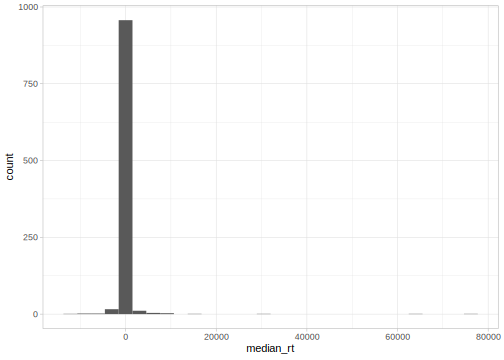
\includegraphics{bookdown_files/figure-latex/priorbeta-1.pdf}
\caption{\label{fig:priorbeta}Prior predictive distribution of the median effect of
the model defined in \ref{sec:trial} with \(\beta \sim Normal(0, 1)\).}
\end{figure}

We repeat the same procedure with \(\beta \sim Normal(0,.01)\), and we
plot it in Figure \ref{fig:priorbeta2}. The prior predictive
distribution shows us that the prior is still quite vague, it is,
however at least in the right order of magnitude. Notice that we are
using a distribution of medians because they are less affected by the
variance in the posterior predicted distribution; distributions of means
will have much more spread. If we want to make the distribution of means
more realistic, we would also need to find a more accurate prior for the
scale, \(\sigma\).




\begin{figure}
\centering
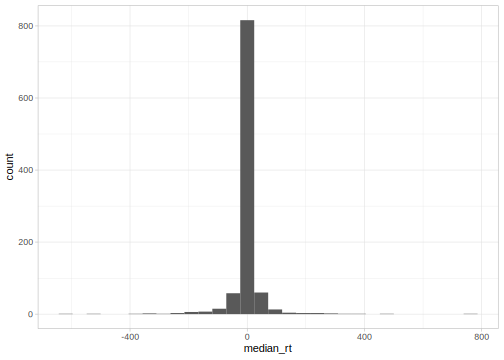
\includegraphics{bookdown_files/figure-latex/priorbeta2-1.pdf}
\caption{\label{fig:priorbeta2}Prior predictive distribution of the median effect of
the model defined in \ref{sec:trial} with \(\beta \sim Normal(0, .01)\).}
\end{figure}

Prior selection might look daunting and a lot of work. However, this
work is usually done only the first time we encounter an experimental
paradigm; besides, priors can be informed by the estimates from previous
experiments (even maximum likelihood estimates from frequentist models
can be useful). We will generally use very similar (or identical priors)
for analyses dealing with the same type of task. When in doubt, a
sensitivity analysis (see section \ref{sec:sensitivity}) can tell us
whether the posterior distribution depends unintentionally strongly on
our prior selection.

\Begin{extra}

\begin{theorem}
\protect\hypertarget{thm:lognormal}{}{\label{thm:lognormal}
}\textbf{Understanding the Log-normal likelihood}
\end{theorem}

It is important to understand what we are assuming with our log-normal
likelihood. Formally, if a random variable \(Y\) is normally distributed
with mean \(\mu\) and variance \(\sigma^2\), then the transformed random
variable \(V = \exp(Y)\) is log-normally distributed and has density:

\begin{equation}
LogNormal(v|\mu,\sigma)=f(y)= \frac{1}{\sqrt{2\pi \sigma^2}v} \exp \left(-\frac{(\log(v)-\mu)^2}{2\sigma^2} \right)
\end{equation}

As explained in section \ref{sec:lnfirst}, the model from
\eqref{eq:rtloglik} is equivalent to the following:

\begin{equation}
\log(rt_n) \sim Normal(\alpha + c\_trial_n \cdot \beta,\sigma)\\
\end{equation}

This, in turn, can be written as follows (see \ref{sec:something}):

\begin{equation}
\log(rt_n) \sim Normal(\alpha, \sigma) + c\_trial_n \cdot \beta
\label{eq:rtlogliknoncen}
\end{equation}

We exponentiate both sides, and we use the property of exponents that
\(\exp(x+y)\) is equivalent to \(\exp(x) \cdot exp(y)\).

\begin{equation}
\begin{aligned}
rt_n &\sim \exp \big(Normal(\alpha, \sigma)  + c\_trial_n \cdot \beta\big) \\
rt_n &\sim \exp\big(Normal(\alpha, \sigma)\big)   \cdot \exp\big(c\_trial_n \cdot \beta\big) \\
rt_n &\sim LogNormal(\alpha, \sigma)   \cdot \exp\big(c\_trial_n \cdot \beta\big) 
\end{aligned}
\end{equation}

So, essentially, we are assuming that reaction times are log-normally
distributed with a median of \(\exp(\alpha)\) and that the effect of
trial number is multiplicative and grows or decays exponentially with
the trial number. This has two important consequences:

\begin{enumerate}
\def\labelenumi{\arabic{enumi}.}
\tightlist
\item
  Different values of the intercept, \(\alpha\), given the same
  \(\beta\), will affect the difference in reaction times for two
  adjacent trials (this is in contrast to what happens with an additive
  model such as normal likelihood); see Figure \ref{fig:logexp}. This is
  because, unlike in the additive case, the intercept doesn't cancel
  out:
\end{enumerate}

\begin{itemize}
\item
  Additive case:

  \begin{equation}
   \begin{aligned}
   & (\alpha + trial_n \cdot \beta) - (\alpha + trial_{n-1} \cdot \beta) = \\
   &=\alpha -\alpha + ( trial_n - trial_{n-1} ) \cdot \beta\\
   &= ( trial_n - trial_{n-1} ) \cdot \beta
   \end{aligned}
   \end{equation}
\item
  Multiplicative case:

  \begin{equation}
   \begin{aligned}
      &\exp(\alpha) \cdot \exp(trial_n \cdot \beta) -\exp(\alpha) \cdot \exp(trial_{n-1} \cdot \beta) =\\ 
      &= \exp(\alpha) \big(\exp(trial_n  \cdot \beta)  - \exp(trial_{n-1}\cdot \beta) \big)\\
      &= \exp(\alpha) \big(\exp(trial_n)  - \exp(trial_{n-1}  \big) \cdot \exp(\beta)\\
      &\neq \big(\exp(trial_n)  - \exp(trial_{n-1}  \big) \cdot \exp(\beta) 
   \end{aligned}
      \end{equation}
\end{itemize}






\begin{figure}[H]
  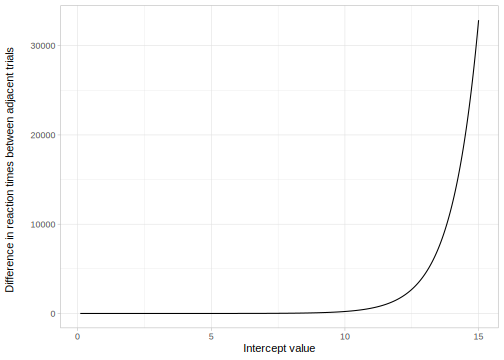
\includegraphics{bookdown_files/figure-latex/logexp-1} \caption{Fitted value of the difference in reaction time between two
adjacent trials, when \(\beta=0.01\) and \(\alpha\) lies between 0.1 and
15. The graph shows how changes in the intercept lead to changes in the
difference in reaction times between trials, even if \(\beta\) is fixed.}\label{fig:logexp}
  \end{figure}

\begin{enumerate}
\def\labelenumi{\arabic{enumi}.}
\setcounter{enumi}{1}
\tightlist
\item
  As the trial number increases, the same value of \(\beta\) will have a
  very different impact on the original scale of the dependent variable:
  \(\beta <0\) will lead to exponential decay and \(\beta >0\) will lead
  to exponential growth; see figure \ref{fig:expgd}.
\end{enumerate}





\begin{figure}[H]
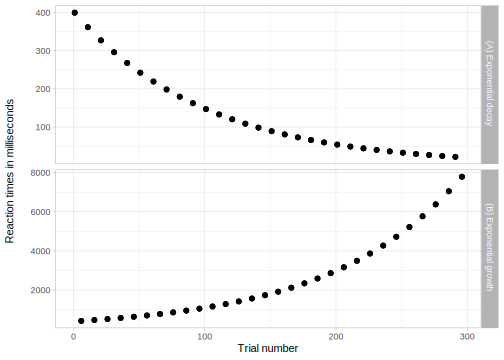
\includegraphics{bookdown_files/figure-latex/expgd-1} \caption{Fitted value of the dependent variable (reaction times in
ms) as function of trial number, when (A) \(\beta = -0.01\), exponential
decay, and when (B) \(\beta =.01\), exponential growth.}\label{fig:expgd}
\end{figure}

Can exponential growth or decay make sense? We need to consider that if
they do make sense, they will be an approximation valid for a specific
range of values, at some point we will expect a ceiling or a floor
effect: reaction times cannot truly be 0 milliseconds, or take minutes.
However, in our specific model, exponential growth or decay \emph{by
trial} is probably a bad approximation: We will predict that our
participant will take extremely long (if \(\beta >0\)) or extremely
short (if \(\beta <0\)) time in pressing the space bar in a relatively
low number of trials. This doesn't mean that the likelihood is wrong by
itself, but it does mean that at least we need to put a cap on the
growth or decay of our experimental manipulation. We can do this if the
exponential growth or decay is a function of, for example,
log-transformed trial numbers:

\begin{equation}
rt_n \sim LogNormal(\alpha + c\_\log\_trial_n) \cdot \beta,\sigma)\\
\end{equation}






\begin{figure}[H]
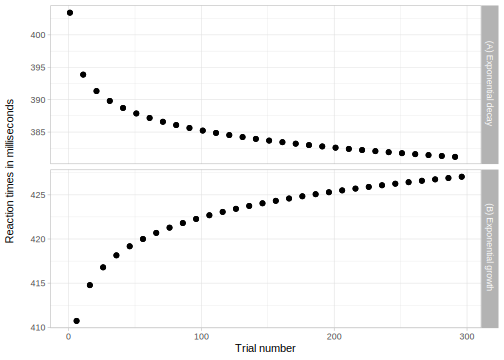
\includegraphics{bookdown_files/figure-latex/expgd2-1} \caption{Fitted value of the dependent variable (reaction times in
ms) as function of the natural logarithm of the trial number, when (A)
\(\beta=-0.01\), exponential decay, and when (B) \(\beta =.01\),
exponential growth.}\label{fig:expgd2}
\end{figure}

\textbf{Log-normal distributions all the way down}

The normal distribution is most often assumed to describe the random
variation that occurs in the data from many scientific disciplines.
However, most measurements actually show skewed distributions.
\citet{limpertLognormalDistributionsSciences2001} discuss the log-normal
distribution in scientific disciplines and how diverse type of data,
from lengths of latent periods of infectious diseases to distribution of
mineral resources in the Earth's crust, including even body height--the
quintessential example of a normal distribution--, closely fit the
log-normal distribution.

\citet{limpertLognormalDistributionsSciences2001} point out that because
a random variable that results from multiplicating many independent
variables has an approximate log-normal distribution, the most basic
indicator of the importance of the log-normal distribution may be very
general: Chemistry and physics are fundamental in life, and the
prevailing operation in the laws of these disciplines is multiplication
rather than addition.

Furthermore, at many physiological and anatomical levels in the brain,
the distribution of numerous parameters is in fact strongly skewed with
a heavy tail, suggesting that skewed (typically log-normal)
distributions are fundamental to structural and functional brain
organization. This might be explained given that the majority of
interactions in highly interconnected systems, especially in biological
systems, are multiplicative and synergistic rather than additive
\citep{buzsakiLogdynamicBrainHow2014}.

Does the log-normal distribution make sense for reaction times? It has
been long noticed that the log-normal distribution often provides a good
fit to reaction times distributions
\citep{breeDistributionProblemsolvingTimes1975, ulrichEffectsTruncationReaction1994}.
One advantage of assuming log-normally distributed reaction times (but,
in fact, this is true for many skewed distributions), is that it entails
that the standard deviation of the reaction time distribution will
increases with the mean, as has been observed in empirical distributions
of reaction times \citep{wagenmakersRelationMeanVariance2005}.
Interestingly, it turns out that log-normal reaction times are also
easily generated by certain process models.
\citet{ulrichInformationProcessingModels1993} show, for example, that
models in which reaction times are determined by a series of processes
cascading activation from an input level to an output level (usually
passing through a number of intervening processing levels along the way)
can generate log-normally distributed reaction times.

\End{extra}

\subsection{\texorpdfstring{The \texttt{brms}
model}{The brms model}}\label{the-brms-model-1}

We are now relatively satisfied with the priors for our model, and we
can fit the data with \texttt{brms}. Notice that we need to specify that
the family is \texttt{lognormal()}.

\begin{Shaded}
\begin{Highlighting}[]
\NormalTok{df_noreading_data <-}\StringTok{ }\KeywordTok{read_csv}\NormalTok{(}\StringTok{"./data/button_press.csv"}\NormalTok{)}
\NormalTok{df_noreading_data <-}\StringTok{ }\NormalTok{df_noreading_data }\OperatorTok
\StringTok{    }\KeywordTok{mutate}\NormalTok{(}\DataTypeTok{c_trial =}\NormalTok{ trialn }\OperatorTok{-}\StringTok{ }\KeywordTok{mean}\NormalTok{(trialn))}

\NormalTok{fit_press_trial <-}\StringTok{ }\KeywordTok{brm}\NormalTok{(rt }\OperatorTok{~}\StringTok{ }\DecValTok{1} \OperatorTok{+}\StringTok{ }\NormalTok{c_trial,}
  \DataTypeTok{data =}\NormalTok{ df_noreading_data,}
  \DataTypeTok{family =} \KeywordTok{lognormal}\NormalTok{(),}
  \DataTypeTok{prior =} \KeywordTok{c}\NormalTok{(}
    \KeywordTok{prior}\NormalTok{(}\KeywordTok{normal}\NormalTok{(}\DecValTok{6}\NormalTok{, }\FloatTok{1.5}\NormalTok{), }\DataTypeTok{class =}\NormalTok{ Intercept),}
    \KeywordTok{prior}\NormalTok{(}\KeywordTok{normal}\NormalTok{(}\DecValTok{0}\NormalTok{, }\DecValTok{1}\NormalTok{), }\DataTypeTok{class =}\NormalTok{ sigma),}
    \KeywordTok{prior}\NormalTok{(}\KeywordTok{normal}\NormalTok{(}\DecValTok{0}\NormalTok{, }\FloatTok{.01}\NormalTok{), }\DataTypeTok{class =}\NormalTok{ b, }\DataTypeTok{coef =}\NormalTok{ c_trial)}
\NormalTok{  )}
\NormalTok{)}
\end{Highlighting}
\end{Shaded}

Instead of printing out the complete output from the model, look at the
estimates from the posteriors for the parameters \(\alpha\), \(\beta\),
and \(\sigma\). Notice that these parameters are on the log scale:

\begin{Shaded}
\begin{Highlighting}[]
\KeywordTok{posterior_summary}\NormalTok{(fit_press_trial)[,}\KeywordTok{c}\NormalTok{(}\StringTok{"Estimate"}\NormalTok{,}\StringTok{"Q2.5"}\NormalTok{,}\StringTok{"Q97.5"}\NormalTok{)]}
\end{Highlighting}
\end{Shaded}

\begin{verbatim}
##                 Estimate         Q2.5        Q97.5
## b_Intercept     5.118349     5.105267     5.131714
## b_c_trial       0.000525     0.000405     0.000649
## sigma           0.123252     0.114256     0.133375
## lp__        -1603.747598 -1607.095317 -1602.289668
\end{verbatim}

The posterior distributions can be plotted to obtain a graphical summary
of all the parameters in the model:

\begin{Shaded}
\begin{Highlighting}[]
\KeywordTok{plot}\NormalTok{(fit_press_trial)}
\end{Highlighting}
\end{Shaded}

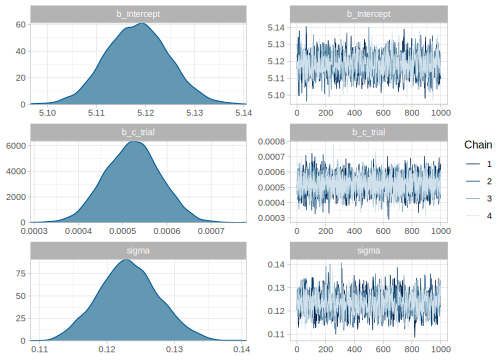
\includegraphics{bookdown_files/figure-latex/unnamed-chunk-112-1.pdf}

Next, we turn to the question of what we can report as our results, and
what we can conclude from the data.

\subsection{How to communicate the
results?}\label{how-to-communicate-the-results-1}

As shown above, the first step is to summarize the posteriors in a table
or graphically (or both). If the research relates to the effect
estimated by the model, the posterior of \(\beta\) can be summarized in
the following way: \(\hat\beta = 0.00053\), 95\% CrI =
\([ 0.00041 , 0.00065 ]\).

But in most cases, the effect is easier to interpret in milliseconds. We
can transform the estimates back to the millisecond scale from the log
scale, but we need to take into account that the scale is not linear,
and that the effect between two button presses will differ depending on
where we are in the experiment.

We will have a different estimate if we consider the difference between
reaction times in a trial at the middle of the experiment (when the
centered trial number is zero) and the previous one (when the centered
trial number is minus one).

\begin{Shaded}
\begin{Highlighting}[]
\NormalTok{alpha_samples <-}\StringTok{ }\KeywordTok{posterior_samples}\NormalTok{(fit_press_trial)}\OperatorTok{$}\NormalTok{b_Intercept}
\NormalTok{beta_samples <-}\StringTok{ }\KeywordTok{posterior_samples}\NormalTok{(fit_press_trial)}\OperatorTok{$}\NormalTok{b_c_trial}
\NormalTok{effect_middle_ms <-}\StringTok{ }\KeywordTok{exp}\NormalTok{(alpha_samples) }\OperatorTok{-}\StringTok{ }\KeywordTok{exp}\NormalTok{(alpha_samples }\OperatorTok{-}\StringTok{ }\DecValTok{1}\OperatorTok{*}\StringTok{ }\NormalTok{beta_samples)}
\NormalTok{## ms effect in the middle of the expt (mean trial vs. mean trial - 1 ) }
\KeywordTok{c}\NormalTok{(}\DataTypeTok{mean =} \KeywordTok{mean}\NormalTok{(effect_middle_ms), }\KeywordTok{quantile}\NormalTok{(effect_middle_ms, }\KeywordTok{c}\NormalTok{(.}\DecValTok{025}\NormalTok{,.}\DecValTok{975}\NormalTok{)))}
\end{Highlighting}
\end{Shaded}

\begin{verbatim}
##   mean   2.5%  97.5% 
## 0.0877 0.0676 0.1084
\end{verbatim}

than if we consider the difference between the second trial and the
first one:

\begin{Shaded}
\begin{Highlighting}[]
\NormalTok{first_trial <-}\StringTok{ }\KeywordTok{min}\NormalTok{(df_noreading_data}\OperatorTok{$}\NormalTok{c_trial)}
\NormalTok{second_trial <-}\StringTok{ }\KeywordTok{min}\NormalTok{(df_noreading_data}\OperatorTok{$}\NormalTok{c_trial) }\OperatorTok{+}\DecValTok{1}
\NormalTok{effect_beginning_ms <-}\StringTok{ }\KeywordTok{exp}\NormalTok{(alpha_samples}\OperatorTok{+}\StringTok{  }\NormalTok{second_trial }\OperatorTok{*}\StringTok{ }\NormalTok{beta_samples) }\OperatorTok{-}
\StringTok{    }\KeywordTok{exp}\NormalTok{(alpha_samples}\OperatorTok{+}\StringTok{  }\NormalTok{first_trial }\OperatorTok{*}\StringTok{ }\NormalTok{beta_samples)}
\NormalTok{## ms effect from first to second trial:}
\KeywordTok{c}\NormalTok{(}\DataTypeTok{mean =} \KeywordTok{mean}\NormalTok{(effect_beginning_ms), }\KeywordTok{quantile}\NormalTok{(effect_beginning_ms, }\KeywordTok{c}\NormalTok{(.}\DecValTok{025}\NormalTok{,.}\DecValTok{975}\NormalTok{)))}
\end{Highlighting}
\end{Shaded}

\begin{verbatim}
##   mean   2.5%  97.5% 
## 0.0797 0.0628 0.0964
\end{verbatim}

There is a slowdown in both cases; when reporting the results of these
analyses, one could present the posterior mean and the 95\% credible
interval and then reason about whether the observed estimates are
consistent with the prediction from the theory being investigated.

The practical relevance of the effect for the research question can be
important too. For example, only after 100 button presses do we see a
slowdown of 9 ms on average (\(0.088 \cdot 100\)), with a 95\% credible
interval ranging from 6.755 to 10.837. We need to consider whether our
uncertainty of this estimate, and the estimated mean effect have any
scientific relevance. Such relevance can be established by considering
the previous literature, predictions from a quantitative model, or other
expert domain knowledge. Sometimes, a quantitative meta-analysis is
helpful; for examples, see \citet{JaegerEngelmannVasishth2017},
\citet{mahowald2016meta}, \citet{NicenboimRoettgeretal}, and
\citet{vasishthProcessingChineseRelative2013}. We will discuss concrete
examples later in the book, in chapters \ref{ch:remame}.

Sometimes, researchers are only interested in establishing that there is
an effect; the magnitude and uncertainty of the estimate is of secondary
interest. Here, the goal is to argue that there is \textbf{evidence} of
a slowdown. The word evidence has a special meaning in statistics
\citep{Royall}, and in null hypothesis significance testing, a
likelihood ratio test is the standard way to argue that one has evidence
for an effect. In the Bayesian data analysis context, a Bayes factor
hypothesis test must be carried out. We'll come back to this issue in
the model comparison chapters \ref{ch:comparison}-\ref{ch:cv}.

\section{Logistic regression: Does set size affect free
recall?}\label{sec:logistic}

We'll look at the capacity limit of working memory to illustrate how the
principles we have learned so far can naturally extend to
\emph{generalized} linear models (GLMs). In this section, we focus on
one special case of GLMs, logistic regression.

For this example, we'll use a subset of the data of
\citet{oberauerWorkingMemoryCapacity2019} from
\url{https://osf.io/qy5sd/}. We'll focus on one subject who was
presented word lists of varying lengths (2, 4, 6, and 8 elements), and
then was asked to recall a word given its position on the list; see
Figure \ref{fig:oberauer}.\footnote{We will only use data from the
  recall test in which the participant had to type the probed word (and
  we will ignore the trials with multiple forced choice for ease of
  explanation).}





\begin{figure}
\includegraphics[width=1\linewidth]{cc_figure/fig1_oberauer_2019_modified} \caption{Flow of events in a trial with memory set size 4 and free
recall. Adapted from \citet{oberauerWorkingMemoryCapacity2019}; licensed
under CC BY 4.0.}\label{fig:oberauer}
\end{figure}

It is well established that as the number of items to be held in working
memory increases, performance, that is accuracy, decreases \citep[among
others][]{oberauerkliegel2001}. We will investigate whether we can
establish this finding with data from only one subject.

\begin{Shaded}
\begin{Highlighting}[]
\NormalTok{df_recall_data <-}\StringTok{ }\KeywordTok{read_csv}\NormalTok{(}\StringTok{"./data/PairsRSS1_all.csv"}\NormalTok{) }\OperatorTok
\StringTok{    }\CommentTok{# We ignore the type of incorrect responses (the focus of the paper)}
\StringTok{    }\KeywordTok{mutate}\NormalTok{(}\DataTypeTok{correct =} \KeywordTok{if_else}\NormalTok{(response_category }\OperatorTok{==}\DecValTok{1}\NormalTok{, }\DecValTok{1}\NormalTok{, }\DecValTok{0}\NormalTok{)) }\OperatorTok
\StringTok{    }\CommentTok{# and we only use the data from the free recall task:}
\StringTok{    }\CommentTok{# (when there was no list of possible responses)}
\StringTok{    }\KeywordTok{filter}\NormalTok{(response_size_list }\OperatorTok{+}\StringTok{ }\NormalTok{response_size_new_words }\OperatorTok{==}\StringTok{ }\DecValTok{0}\NormalTok{) }\OperatorTok
\StringTok{    }\CommentTok{# We select one subject}
\StringTok{    }\KeywordTok{filter}\NormalTok{(subject }\OperatorTok{==}\StringTok{ }\DecValTok{10}\NormalTok{) }\OperatorTok
\StringTok{    }\KeywordTok{mutate}\NormalTok{(}\DataTypeTok{c_set_size =}\NormalTok{ set_size }\OperatorTok{-}\StringTok{ }\KeywordTok{mean}\NormalTok{(set_size)) }\OperatorTok
\StringTok{    }\KeywordTok{select}\NormalTok{(subject, set_size, c_set_size, correct, trial, session, block, tested)}

\CommentTok{# we can ignore the warning from read_table}

\CommentTok{# Set sizes in the dataset:}
\NormalTok{df_recall_data}\OperatorTok{$}\NormalTok{set_size }\OperatorTok
\StringTok{    }\NormalTok{unique}
\end{Highlighting}
\end{Shaded}

\begin{verbatim}
## [1] 4 8 2 6
\end{verbatim}

\begin{Shaded}
\begin{Highlighting}[]
\CommentTok{# Trials by set size}
\NormalTok{df_recall_data }\OperatorTok
\StringTok{    }\KeywordTok{group_by}\NormalTok{(set_size) }\OperatorTok
\StringTok{    }\KeywordTok{count}\NormalTok{()}
\end{Highlighting}
\end{Shaded}

\begin{verbatim}
## # A tibble: 4 x 2
## # Groups:   set_size [4]
##   set_size     n
##      <dbl> <int>
## 1        2    23
## 2        4    23
## 3        6    23
## 4        8    23
\end{verbatim}

The data look like this: the column \texttt{correct} records the 0
(incorrect) or 1 (correct) responses, and the column
\texttt{c\_set\_size} records the centered memory set size; these latter
scores have continuous values -3, -1, 1, and 3. These continuous values
are centered versions of 2, 4, 6, and 8.

\begin{Shaded}
\begin{Highlighting}[]
\NormalTok{df_recall_data}
\end{Highlighting}
\end{Shaded}

\begin{verbatim}
## # A tibble: 92 x 8
##   subject set_size c_set_size correct trial session block tested
##     <dbl>    <dbl>      <dbl>   <dbl> <dbl>   <dbl> <dbl>  <dbl>
## 1      10        4         -1       1     1       1     1      2
## 2      10        8          3       0     4       1     1      8
## 3      10        2         -3       1     9       1     1      2
## 4      10        6          1       1    23       1     1      2
## 5      10        4         -1       1     5       1     2      3
## # ... with 87 more rows
\end{verbatim}

We want to model the trial by trial accuracy and examine whether the
probability of recalling a word is related to the number of words in the
set that the subject needs to remember.

\subsection{The likelihood for the logistic regression
model}\label{the-likelihood-for-the-logistic-regression-model}

Recall that the Bernoulli likelihood generates a 0 or 1 response with a
particular probability \(\theta\). For example, one can generate
simulated data for 10 trials, with 50\% chances of getting a one as
follows:

\begin{Shaded}
\begin{Highlighting}[]
\NormalTok{extraDistr}\OperatorTok{::}\KeywordTok{rbern}\NormalTok{(}\DecValTok{10}\NormalTok{, }\DataTypeTok{prob =} \FloatTok{0.5}\NormalTok{)}
\end{Highlighting}
\end{Shaded}

\begin{verbatim}
##  [1] 1 1 0 1 0 1 1 1 1 0
\end{verbatim}

We can therefore define each dependent value \texttt{correct\_n} in the
data as being generated from a Bernoulli random variable with
probability of success \(\theta_n\). Here, \(n =1, \ldots, N\) indexes
the trial, correct\_n is the dependent variable (0 indicates an
incorrect recall and 1 a correct recall), and \(\theta_n\) is the
probability of correctly recalling a probe in a given trial \(n\).

\begin{equation}
correct_n \sim Bernoulli(\theta_n)
\label{eq:bernoullilik}
\end{equation}

Since \(\theta_n\) is bounded to be between 0 and 1 (it is a
probability), we cannot just fit a regression model using the normal or
lognormal likelihood as we did in the preceding examples. Such a model
would be inappropriate because it would assume that the data range from
\(-\infty\) to \(+\infty\), rather than from 0 to 1.

The generalized linear modeling framework solves this problem by
defining a so-called \emph{link function} \(g(\cdot)\) that connects the
linear model to the quantity to be estimated (here, the probabilities
\(\theta_n\)). The link function used for 0,1 responses is called the
\emph{logit link}, and is defined as follows.

\begin{equation}
\eta_n = g(\theta_n) = \log\left(\frac{\theta_n}{1-\theta_n}\right)
\end{equation}

The term \(\frac{\theta_n}{1-\theta_n}\) is called the
\emph{odds}.\footnote{Odds are defined to be the ratio of the
  probability of success to the probability of failure. For example, the
  odds of obtaining a one in a fair six-sided die are
  \(\frac{1/6}{1-1/6}=1/5\). The odds of obtaining a heads in a fair
  coin are 1/1.} The logit link function is therefore a log-odds; it
maps probability values ranging from \([0,1]\) to real numbers ranging
from \((-\infty,+\infty)\). Figure \ref{fig:logisticfun} shows the logit
link function, \(\eta = g(\theta)\), and the inverse logit,
\(\theta = g^{-1}(\eta)\), which is called the \textbf{logistic
function}; the relevance of this logistic function will become clear in
a moment.

\begin{figure}
\centering
\includegraphics{bookdown_files/figure-latex/logisticfun-1.pdf}
\caption{\label{fig:logisticfun}The logit and inverse logit (logistic)
function.}
\end{figure}

The linear model is now fit not to the 0,1 responses as the dependent
variable, but to \(\eta_n\), i.e., log-odds, as the dependent variable:

\begin{equation}
\eta_n = \log\left(\frac{\theta_n}{1-\theta_n}\right) = \alpha + \beta \cdot c\_set\_size
\end{equation}

Once \(\eta_n\) is estimated, one can solve the above equation for
\(\theta_n\) (in other words, we compute the inwverse of the logit
function). This gives the above-mentioned logistic regression function:

\begin{equation}
\theta_n = g^{-1}(\eta_n) =  \log\left(\frac{\exp(\eta_n)}{1+\exp(\eta_n)}\right)
\end{equation}

In summary, the generalized linear model with the logit link fits the
following Bernoulli likelihood:

\begin{equation}
correct_n \sim Bernoulli(\theta_n)
\label{eq:bernoullilogislik}
\end{equation}

The model is fit on the log-odds scale,
\(\eta_n = \alpha + c\_set\_size_n \cdot \beta\). Once \(\eta_n\) has
been estimated, the inverse logit or the logistic function is used to
compute the probability estimates
\(\theta_n = \log(\frac{\exp(\eta_n)}{1+\exp(\eta_n)})\). An example of
the calculations will be shown in the next section.

\subsection{Priors for the logistic
regression}\label{priors-for-the-logistic-regression}

In order to decide on priors for \(\alpha\) and \(\beta\) we need to
take into account that these parameter do not represent probabilities or
proportions, but \emph{log-odds}, the x-axis in Figure
\ref{fig:logisticfun} (right-hand side figure). As shown in the figure,
the relationship between log-odds and probabilities is not linear.

There are two functions in R that implement the logit and inverse logit
functions: \texttt{qlogis(p)} for the logit function and
\texttt{plogis(x)} for the inverse logit or logistic function.

Now we need to set priors for \(\alpha\) and \(\beta\). Given that we
centered our predictor, the intercept, \(\alpha\), represents the
log-odds of correctly recalling one word in a random position for the
average set size of five (since \(5 = \frac{2+4+6+8}{4}\)), which,
incidentally, was not presented in the experiment. This is one case
where the intercept doesn't have a clear interpretation if we leave the
prediction uncentered: With non-centered set size, the intercept will be
the log-odds of recalling one word in a set of \emph{zero} words.

The prior for \(\alpha\) will depend on how difficult the recall task
is. If we are not sure, we could assume that the probability of
recalling a word for an average set size, \(\alpha\), is centered in .5
(a 50/50 chance) with a great deal of uncertainty. The \texttt{R}
command \texttt{qlogis(.5)} tells us that .5 corresponds to zero in
log-odds. How do we include a great deal of uncertainty? We could look
at Figure \ref{fig:logisticfun}, and decide on a standard deviation of 4
in a normal distribution centered in zero:

\begin{equation}
\alpha \sim Normal(0, 4) 
\end{equation}

Let's plot this prior in log-odds and in probability scale by drawing
random samples.




\begin{Shaded}
\begin{Highlighting}[]
\NormalTok{samples_logodds <-}\StringTok{ }\KeywordTok{tibble}\NormalTok{(}\DataTypeTok{alpha =} \KeywordTok{rnorm}\NormalTok{(}\DecValTok{100000}\NormalTok{, }\DecValTok{0}\NormalTok{, }\DecValTok{4}\NormalTok{))}
\NormalTok{samples_prob <-}\StringTok{ }\KeywordTok{tibble}\NormalTok{(}\DataTypeTok{p =} \KeywordTok{plogis}\NormalTok{(}\KeywordTok{rnorm}\NormalTok{(}\DecValTok{100000}\NormalTok{, }\DecValTok{0}\NormalTok{, }\DecValTok{4}\NormalTok{)))}
\KeywordTok{ggplot}\NormalTok{(samples_logodds, }\KeywordTok{aes}\NormalTok{(alpha)) }\OperatorTok{+}
\StringTok{    }\KeywordTok{geom_density}\NormalTok{()}
\KeywordTok{ggplot}\NormalTok{(samples_prob, }\KeywordTok{aes}\NormalTok{(p)) }\OperatorTok{+}
\StringTok{    }\KeywordTok{geom_density}\NormalTok{()}
\end{Highlighting}
\end{Shaded}

\begin{figure}
\includegraphics[width=0.45\linewidth]{bookdown_files/figure-latex/logoddspriorsf-1} \includegraphics[width=0.45\linewidth]{bookdown_files/figure-latex/logoddspriorsf-2} \caption{Prior for \(\alpha \sim Normal(0, 4)\) in log-odds
and in probability space.}\label{fig:logoddspriorsf}
\end{figure}

Figure \ref{fig:logoddspriorsf} shows that our prior assigns more
probability mass to extreme probabilities of recall than to intermediate
values. Clearly, this is not what we intended.

We could try several values for standard deviation of the prior, until
we find a prior that make sense for us. Reducing the standard deviation
to 1.5 seems to make sense as shown in Figure \ref{fig:logoddspriorsf2}.

\begin{equation}
\alpha \sim Normal(0, 1.5) 
\end{equation}




\begin{figure}
\includegraphics[width=0.45\linewidth]{bookdown_files/figure-latex/logoddspriorsf2-1} \includegraphics[width=0.45\linewidth]{bookdown_files/figure-latex/logoddspriorsf2-2} \caption{Prior for \(\alpha \sim Normal(0, 1.5)\) in
log-odds and in probability space.}\label{fig:logoddspriorsf2}
\end{figure}

We need to decide now on the prior for the effect in log-odds of
increasing the set size, \(\beta\). We are going to choose a normal
distribution centered on zero, reflecting our lack of any commitment
regarding the direction of the effect. Let's get some intuitions
regarding different possible standard deviations for this prior, by
testing the following distributions as priors:

\begin{enumerate}
\def\labelenumi{(\alph{enumi})}
\tightlist
\item
  \(\beta \sim Normal(0, 1)\)
\item
  \(\beta \sim Normal(0, .5)\)
\item
  \(\beta \sim Normal(0, .1)\)
\item
  \(\beta \sim Normal(0, .01)\)
\item
  \(\beta \sim Normal(0, .001)\)
\end{enumerate}

The following function is an edited version of the earlier
\texttt{normal\_predictive\_distribution\_fast} from section
\ref{sec:ppd}; it has been edited to make it compatible with logistic
regression and dependent on set size:

\begin{Shaded}
\begin{Highlighting}[]
\NormalTok{logistic_model_pred <-}\StringTok{ }\ControlFlowTok{function}\NormalTok{(alpha_samples,}
\NormalTok{                                beta_samples,}
\NormalTok{                                set_size,}
\NormalTok{                                 N_obs) \{}
    \KeywordTok{map2_dfr}\NormalTok{(alpha_samples, beta_samples,}
             \ControlFlowTok{function}\NormalTok{(alpha, beta) \{}
                 \KeywordTok{tibble}\NormalTok{(}
                     \DataTypeTok{set_size =}\NormalTok{ set_size,}
                     \CommentTok{# we center size:}
                     \DataTypeTok{c_set_size =}\NormalTok{ set_size }\OperatorTok{-}\StringTok{ }\KeywordTok{mean}\NormalTok{(set_size),}
                     \CommentTok{# change the likelihood: }
                     \CommentTok{# Notice the use of a link function for alpha and beta}
                     \DataTypeTok{theta =} \KeywordTok{plogis}\NormalTok{(alpha }\OperatorTok{+}\StringTok{ }\NormalTok{c_set_size }\OperatorTok{*}\StringTok{ }\NormalTok{beta),}
                     \DataTypeTok{correct_pred =} \KeywordTok{rbernoulli}\NormalTok{(N_obs,  }\DataTypeTok{p =}\NormalTok{ theta)}
\NormalTok{                 )}
\NormalTok{             \}, }\DataTypeTok{.id =} \StringTok{"iter"}\NormalTok{) }\OperatorTok
\StringTok{    }\CommentTok{# .id is always a string and needs to be converted to a number}
\StringTok{        }\KeywordTok{mutate}\NormalTok{(}\DataTypeTok{iter =} \KeywordTok{as.numeric}\NormalTok{(iter))}
\NormalTok{\}}
\end{Highlighting}
\end{Shaded}

Let's assume 800 observations with 200 observation of each set size:

\begin{Shaded}
\begin{Highlighting}[]
\NormalTok{N_obs <-}\StringTok{ }\DecValTok{800}
\NormalTok{set_size <-}\StringTok{ }\KeywordTok{rep}\NormalTok{(}\KeywordTok{c}\NormalTok{(}\DecValTok{2}\NormalTok{,}\DecValTok{4}\NormalTok{,}\DecValTok{6}\NormalTok{,}\DecValTok{8}\NormalTok{),}\DecValTok{200}\NormalTok{)}
\end{Highlighting}
\end{Shaded}

We iterate over the four possible standard deviations of \(\beta\):

\begin{Shaded}
\begin{Highlighting}[]
\NormalTok{alpha_samples <-}\StringTok{ }\KeywordTok{rnorm}\NormalTok{(}\DecValTok{1000}\NormalTok{, }\DecValTok{0}\NormalTok{, }\FloatTok{1.5}\NormalTok{)}
\NormalTok{sds_beta <-}\StringTok{ }\KeywordTok{c}\NormalTok{(}\DecValTok{1}\NormalTok{, }\FloatTok{0.5}\NormalTok{, }\FloatTok{0.1}\NormalTok{,}\FloatTok{0.01}\NormalTok{, }\FloatTok{0.001}\NormalTok{) }
\NormalTok{prior_pred <-}\StringTok{ }\KeywordTok{map_dfr}\NormalTok{(sds_beta, }\ControlFlowTok{function}\NormalTok{(sd) \{}
\NormalTok{    beta_samples <-}\StringTok{ }\KeywordTok{rnorm}\NormalTok{(}\DecValTok{1000}\NormalTok{, }\DecValTok{0}\NormalTok{, sd)}
    \KeywordTok{logistic_model_pred}\NormalTok{(}\DataTypeTok{alpha_samples =}\NormalTok{ alpha_samples,}
                        \DataTypeTok{beta_samples =}\NormalTok{ beta_samples,}
                        \DataTypeTok{set_size =}\NormalTok{ set_size,}
                        \DataTypeTok{N_obs =}\NormalTok{ N_obs}
\NormalTok{                        ) }\OperatorTok
\StringTok{        }\KeywordTok{mutate}\NormalTok{(}\DataTypeTok{prior_beta_sd =}\NormalTok{ sd)}
\NormalTok{\})}
\end{Highlighting}
\end{Shaded}

And we calculate the accuracy for each one of the priors we want to
examine, for each iteration, and for each set size.

\begin{Shaded}
\begin{Highlighting}[]
\NormalTok{mean_accuracy <-}
\StringTok{     }\NormalTok{prior_pred }\OperatorTok
\StringTok{     }\KeywordTok{group_by}\NormalTok{(prior_beta_sd, iter, set_size) }\OperatorTok
\StringTok{     }\KeywordTok{summarize}\NormalTok{(}\DataTypeTok{accuracy =} \KeywordTok{mean}\NormalTok{(correct_pred)) }\OperatorTok
\StringTok{     }\KeywordTok{mutate}\NormalTok{(}\DataTypeTok{prior =} \KeywordTok{paste0}\NormalTok{(}\StringTok{"Normal(0, "}\NormalTok{,prior_beta_sd,}\StringTok{")"}\NormalTok{))}
\end{Highlighting}
\end{Shaded}

We plot it in Figure \ref{fig:priors4beta}, and as expected the priors
are centered at zero. We see that the distribution of possible
accuracies for the prior that has a standard deviation of one is
problematic: There is too much probability mass concentrated near zero
and one for set sizes of 2 and 8.





\begin{Shaded}
\begin{Highlighting}[]
\NormalTok{mean_accuracy }\OperatorTok
\StringTok{    }\KeywordTok{ggplot}\NormalTok{(}\KeywordTok{aes}\NormalTok{(accuracy)) }\OperatorTok{+}
\StringTok{    }\KeywordTok{geom_histogram}\NormalTok{() }\OperatorTok{+}
\StringTok{    }\KeywordTok{facet_grid}\NormalTok{(set_size}\OperatorTok{~}\NormalTok{prior)}
\end{Highlighting}
\end{Shaded}

\begin{figure}
\centering
\includegraphics{bookdown_files/figure-latex/priors4beta-1.pdf}
\caption{\label{fig:priors4beta}Prior predictive distribution of mean accuracy of the
model defined in \ref{sec:logistic}, for different set sizes and
different priors for \(\beta\).}
\end{figure}

It's hard to tell the differences between the other priors, and it might
be more useful to look at the predicted differences in accuracy between
set sizes. We calculate them as follows:

\begin{Shaded}
\begin{Highlighting}[]
\NormalTok{diff_accuracy <-}\StringTok{ }\NormalTok{mean_accuracy }\OperatorTok
\StringTok{    }\KeywordTok{arrange}\NormalTok{(set_size) }\OperatorTok
\StringTok{    }\KeywordTok{group_by}\NormalTok{(iter, prior_beta_sd) }\OperatorTok
\StringTok{    }\KeywordTok{mutate}\NormalTok{(}\DataTypeTok{diffaccuracy =}\NormalTok{ accuracy }\OperatorTok{-}\StringTok{ }\KeywordTok{lag}\NormalTok{(accuracy) ) }\OperatorTok
\StringTok{    }\KeywordTok{mutate}\NormalTok{(}\DataTypeTok{diffsize =} \KeywordTok{paste}\NormalTok{(set_size,}\StringTok{"-"}\NormalTok{,  }\KeywordTok{lag}\NormalTok{(set_size))) }\OperatorTok
\StringTok{    }\KeywordTok{filter}\NormalTok{(set_size }\OperatorTok{>}\DecValTok{2}\NormalTok{)}
\end{Highlighting}
\end{Shaded}





\begin{Shaded}
\begin{Highlighting}[]
\NormalTok{diff_accuracy }\OperatorTok
\StringTok{    }\KeywordTok{ggplot}\NormalTok{(}\KeywordTok{aes}\NormalTok{(diffaccuracy)) }\OperatorTok{+}
\StringTok{    }\KeywordTok{geom_histogram}\NormalTok{() }\OperatorTok{+}
\StringTok{    }\KeywordTok{facet_grid}\NormalTok{(diffsize}\OperatorTok{~}\NormalTok{prior)}
\end{Highlighting}
\end{Shaded}

\begin{figure}
\centering
\includegraphics{bookdown_files/figure-latex/priors4beta2-1.pdf}
\caption{\label{fig:priors4beta2}Prior predictive distribution of differences in mean
accuracy between set sizes of the model defined in \ref{sec:logistic}
for different priors for \(\beta\).}
\end{figure}

We plot them in Figure \ref{fig:priors4beta2}. If we are not sure
whether the increase of set size could produce something between a null
effect and a relatively large effect, we can choose the prior with a
standard deviation of \(0.1\). Thus we settle on the following priors:

\begin{equation}
\begin{aligned}
\alpha &\sim Normal(0, 1.5) \\
\beta &\sim Normal(0, 0.1) 
\end{aligned}
\end{equation}

\subsection{\texorpdfstring{The \texttt{brms}
model}{The brms model}}\label{the-brms-model-2}

Having decided on the likelihood, the link function, and the priors, the
model can now be fit using \texttt{brms}. Notice that we need to specify
that the family is \texttt{bernoulli()}, and the link is \texttt{logit}.

\begin{Shaded}
\begin{Highlighting}[]
\NormalTok{fit_recall <-}\StringTok{ }\KeywordTok{brm}\NormalTok{(correct }\OperatorTok{~}\StringTok{ }\DecValTok{1} \OperatorTok{+}\StringTok{ }\NormalTok{c_set_size,}
  \DataTypeTok{data =}\NormalTok{ df_recall_data,}
  \DataTypeTok{family =} \KeywordTok{bernoulli}\NormalTok{(}\DataTypeTok{link =}\NormalTok{ logit),}
  \DataTypeTok{prior =} \KeywordTok{c}\NormalTok{(}
    \KeywordTok{prior}\NormalTok{(}\KeywordTok{normal}\NormalTok{(}\DecValTok{0}\NormalTok{, }\FloatTok{1.5}\NormalTok{), }\DataTypeTok{class =}\NormalTok{ Intercept),}
    \KeywordTok{prior}\NormalTok{(}\KeywordTok{normal}\NormalTok{(}\DecValTok{0}\NormalTok{, }\FloatTok{.1}\NormalTok{), }\DataTypeTok{class =}\NormalTok{ b, }\DataTypeTok{coef =}\NormalTok{ c_set_size)}
\NormalTok{  )}
\NormalTok{)}
\end{Highlighting}
\end{Shaded}

Next, look at the summary of the posteriors of each of the parameters.
Keep in mind that the parameters are in log-odds space:

\begin{Shaded}
\begin{Highlighting}[]
\KeywordTok{posterior_summary}\NormalTok{(fit_recall, }\DataTypeTok{pars =} \KeywordTok{c}\NormalTok{(}\StringTok{"b_Intercept"}\NormalTok{, }\StringTok{"b_c_set_size"}\NormalTok{))}
\end{Highlighting}
\end{Shaded}

\begin{verbatim}
##              Estimate Est.Error   Q2.5   Q97.5
## b_Intercept     1.919    0.3063  1.344  2.5512
## b_c_set_size   -0.185    0.0815 -0.344 -0.0218
\end{verbatim}

Plot the posteriors as well:

\begin{Shaded}
\begin{Highlighting}[]
\KeywordTok{plot}\NormalTok{(fit_recall)}
\end{Highlighting}
\end{Shaded}

\includegraphics{bookdown_files/figure-latex/unnamed-chunk-126-1.pdf}

Next, we turn to the question of what we can report as our results, and
what we can conclude from the data.

\subsection{How to communicate the results?}\label{sec:comlogis}

We are here in a situation analogous as before with the log-normal
model. If we want to talk about the effect estimated by the model in
log-odds space, we summarize the posterior of \(\beta\) in the following
way: \(\hat\beta = -0.185\), 95\% CrI = \([ -0.344 , -0.022 ]\).

However, the effect might be easier to understand in proportions rather
than in log-odds. Let's look at the average accuracy for the task first:

\begin{Shaded}
\begin{Highlighting}[]
\NormalTok{alpha_samples<-}\StringTok{ }\KeywordTok{posterior_samples}\NormalTok{(fit_recall)}\OperatorTok{$}\NormalTok{b_Intercept}
\NormalTok{av_accuracy <-}\StringTok{ }\KeywordTok{plogis}\NormalTok{(alpha_samples)}
\KeywordTok{c}\NormalTok{(}\DataTypeTok{mean =} \KeywordTok{mean}\NormalTok{(av_accuracy), }\KeywordTok{quantile}\NormalTok{(av_accuracy, }\KeywordTok{c}\NormalTok{(.}\DecValTok{025}\NormalTok{,.}\DecValTok{975}\NormalTok{)))}
\end{Highlighting}
\end{Shaded}

\begin{verbatim}
##  mean  2.5% 97.5% 
## 0.868 0.793 0.928
\end{verbatim}

As before, to transform the effect of our manipulation to an easier to
interpret scale (i.e., proportion), we need to take into account that
the scale is not linear, and that the effect of increasing the set size
depends on the average accuracy, and the set size that we start from.

We can do the following calculation, similar to what we did for the
trial effects experiment, to find out the decrease in accuracy in
proportions or probability scale:

\begin{Shaded}
\begin{Highlighting}[]
\NormalTok{beta_samples<-}\StringTok{ }\KeywordTok{posterior_samples}\NormalTok{(fit_recall)}\OperatorTok{$}\NormalTok{b_c_set_size}
\NormalTok{effect_middle <-}\StringTok{ }\KeywordTok{plogis}\NormalTok{(alpha_samples) }\OperatorTok{-}\StringTok{ }\KeywordTok{plogis}\NormalTok{(alpha_samples }\OperatorTok{-}\StringTok{ }\NormalTok{beta_samples)}
\KeywordTok{c}\NormalTok{(}\DataTypeTok{mean =} \KeywordTok{mean}\NormalTok{(effect_middle), }\KeywordTok{quantile}\NormalTok{(effect_middle, }\KeywordTok{c}\NormalTok{(.}\DecValTok{025}\NormalTok{,.}\DecValTok{975}\NormalTok{)))}
\end{Highlighting}
\end{Shaded}

\begin{verbatim}
##     mean     2.5%    97.5% 
## -0.01903 -0.03680 -0.00256
\end{verbatim}

Notice the interpretation here, if we increase the set size from the
average set size minus one to the average set size, we get a reduction
in the accuracy of recall of \(-0.019\), 95\% CrI =
\([ -0.037 , -0.003 ]\). Recall that the average set size, 5, was not
presented to the subject! We could also look at the decrease in accuracy
from a set size of 2 to 4:

\begin{Shaded}
\begin{Highlighting}[]
\NormalTok{effect_4m2 <-}
\StringTok{  }\KeywordTok{plogis}\NormalTok{(alpha_samples }\OperatorTok{+}\StringTok{ }\NormalTok{(}\DecValTok{4} \OperatorTok{-}\StringTok{ }\KeywordTok{mean}\NormalTok{(df_recall_data}\OperatorTok{$}\NormalTok{set_size)) }\OperatorTok{*}\StringTok{ }\NormalTok{beta_samples) }\OperatorTok{-}
\StringTok{  }\KeywordTok{plogis}\NormalTok{(alpha_samples }\OperatorTok{+}\StringTok{ }\NormalTok{(}\DecValTok{2} \OperatorTok{-}\StringTok{ }\KeywordTok{mean}\NormalTok{(df_recall_data}\OperatorTok{$}\NormalTok{set_size)) }\OperatorTok{*}\StringTok{ }\NormalTok{beta_samples)}
\KeywordTok{c}\NormalTok{(}\DataTypeTok{mean =} \KeywordTok{mean}\NormalTok{(effect_4m2), }\KeywordTok{quantile}\NormalTok{(effect_4m2, }\KeywordTok{c}\NormalTok{(.}\DecValTok{025}\NormalTok{,.}\DecValTok{975}\NormalTok{)))}
\end{Highlighting}
\end{Shaded}

\begin{verbatim}
##     mean     2.5%    97.5% 
## -0.02969 -0.05315 -0.00501
\end{verbatim}

We see that increasing the set size does have a detrimental effect in
recall, as we suspected.

\subsection{Descriptive adequacy}\label{descriptive-adequacy}

One potentially useful aspect of posterior distributions is that we
could also make predictions for other conditions not presented in the
actual experiment, such as set sizes that weren't tested. We could then
verify if our model was right with another experiment. To make
predictions for other set sizes, we extend our dataset adding rows with
set sizes of 3, 5, and 7. To be consistent with the data of the other
set sizes in the experiment, we add 23 trials of each new set size (this
is the number of trial by set sizes in the dataset). Something important
to notice is that \textbf{we need to center our predictor based on the
original mean set size}. This is because we want to maintain our
interpretation of the intercept. We extend the data as follows, and we
summarize the data and plot it in Figure \ref{fig:postpredsum2}.

\begin{Shaded}
\begin{Highlighting}[]
\NormalTok{df_recall_data_ext <-}\StringTok{ }\NormalTok{df_recall_data }\OperatorTok
\StringTok{    }\KeywordTok{bind_rows}\NormalTok{(}\KeywordTok{tibble}\NormalTok{(}\DataTypeTok{set_size =} \KeywordTok{rep}\NormalTok{(}\KeywordTok{c}\NormalTok{(}\DecValTok{3}\NormalTok{, }\DecValTok{5}\NormalTok{, }\DecValTok{7}\NormalTok{), }\DecValTok{23}\NormalTok{),}
                     \DataTypeTok{c_set_size =}\NormalTok{ set_size }\OperatorTok{-}
\StringTok{                       }\KeywordTok{mean}\NormalTok{(df_recall_data}\OperatorTok{$}\NormalTok{set_size)))}
\NormalTok{df_recall_pred_ext <-}
\StringTok{  }\KeywordTok{posterior_predict}\NormalTok{(fit_recall,}
                    \DataTypeTok{newdata =}\NormalTok{ df_recall_data_ext,}
                    \DataTypeTok{nsamples =} \DecValTok{1000}\NormalTok{) }\OperatorTok
\StringTok{  }\KeywordTok{array_branch}\NormalTok{(}\DataTypeTok{margin =} \DecValTok{1}\NormalTok{) }\OperatorTok
\StringTok{  }\KeywordTok{map_dfr}\NormalTok{( }\ControlFlowTok{function}\NormalTok{(yrep_iter) \{}
\NormalTok{    df_recall_data_ext }\OperatorTok
\StringTok{      }\KeywordTok{mutate}\NormalTok{(}\DataTypeTok{correct =}\NormalTok{ yrep_iter)}
\NormalTok{  \}, }\DataTypeTok{.id =} \StringTok{"iter"}\NormalTok{) }\OperatorTok
\StringTok{  }\KeywordTok{mutate}\NormalTok{(}\DataTypeTok{iter =} \KeywordTok{as.numeric}\NormalTok{(iter))}
\end{Highlighting}
\end{Shaded}





\begin{Shaded}
\begin{Highlighting}[]
\NormalTok{df_recall_pred_ext_summary <-}\StringTok{ }\NormalTok{df_recall_pred_ext }\OperatorTok
\StringTok{    }\KeywordTok{group_by}\NormalTok{(iter, set_size) }\OperatorTok
\StringTok{    }\KeywordTok{summarize}\NormalTok{(}\DataTypeTok{accuracy =} \KeywordTok{mean}\NormalTok{(correct))}
\CommentTok{# observed means:}
\NormalTok{df_recall_summary<-}\StringTok{ }\NormalTok{df_recall_data }\OperatorTok
\StringTok{    }\KeywordTok{group_by}\NormalTok{(set_size) }\OperatorTok
\StringTok{    }\KeywordTok{summarize}\NormalTok{(}\DataTypeTok{accuracy =} \KeywordTok{mean}\NormalTok{(correct))}
\KeywordTok{ggplot}\NormalTok{(df_recall_pred_ext_summary, }\KeywordTok{aes}\NormalTok{(accuracy)) }\OperatorTok{+}
\StringTok{    }\KeywordTok{geom_histogram}\NormalTok{(}\DataTypeTok{alpha=}\NormalTok{.}\DecValTok{5}\NormalTok{)}\OperatorTok{+}
\StringTok{    }\KeywordTok{geom_vline}\NormalTok{(}\KeywordTok{aes}\NormalTok{(}\DataTypeTok{xintercept=}\NormalTok{ accuracy),}\DataTypeTok{data=}\NormalTok{ df_recall_summary)}\OperatorTok{+}
\StringTok{    }\KeywordTok{facet_grid}\NormalTok{(set_size }\OperatorTok{~}\StringTok{ }\NormalTok{.)}
\end{Highlighting}
\end{Shaded}

\begin{figure}
\centering
\includegraphics{bookdown_files/figure-latex/postpredsum2-1.pdf}
\caption{\label{fig:postpredsum2}Distribution of posterior predicted mean accuracies
in gray for tested set sizes (2, 4, 6, and 8) and untested ones (3, 5,
and 7), and observed mean accuracy in black lines by tested set sizes.}
\end{figure}

\section{Summary}\label{summary-1}

\section{Further reading}\label{further-reading-3}

\section{Exercises}\label{exercises-2}

\begin{exercise}
\protect\hypertarget{exr:pupils}{}{\label{exr:pupils} }A first linear
regression: Revisitng attentional load effect on pupil size.
\end{exercise}

\begin{enumerate}
\def\labelenumi{\alph{enumi}.}
\tightlist
\item
  Our priors for this experiment were quite arbitrary. How do the prior
  predictive distributions look like? Do they make sense?
\item
  Is our posterior distribution sensitive to the priors that we
  selected? Perform a sensitivity analysis to find out whether the
  posterior is affected by our choice of prior for the \(\sigma\).
\item
  Our dataset includes also a column that indicates the trial number.
  Could it be that trial has also an effect on the pupil size? As in
  \texttt{lm}, we indicate another main effect with a \texttt{+} sign.
  How would you communicate the new results?
\end{enumerate}

\begin{exercise}
\protect\hypertarget{exr:lognormalm}{}{\label{exr:lognormalm} }Log-normal
model: Revisiting the effect of trial on reaction times.
\end{exercise}

\begin{enumerate}
\def\labelenumi{\alph{enumi}.}
\tightlist
\item
  Estimate the slowdown in milliseconds between the last two times the
  subject pressed the space bar in the experiment.
\item
  How would you change your model (keeping the log-normal likelihood) so
  that it includes centered log-transformed trial numbers or
  square-root-transformed trial numbers (instead of centered trial
  numbers)? Does the effect in milliseconds change?
\end{enumerate}

\begin{exercise}
\protect\hypertarget{exr:reg-logistic}{}{\label{exr:reg-logistic} }Logistic
regression: Revisiting the effect of set size on free recall.
\end{exercise}

Our dataset includes also a column coded as \texttt{tested} that
indicates the position of the queued word. (In Figure \ref{fig:oberauer}
\texttt{tested} would be 3). Could it be that the position has also an
effect on the recall accuracy? How would you incorporate this in the
model? Verify the descriptive adequacy of our new model.

\section{Appendix}\label{appendix-1}

\subsection{Preparation of the pupil size data (section
\ref{sec:pupil})}\label{sec:preprocessingpupil}

We prepared the data for the linear model of section \ref{sec:pupil}
with a dataset from \citet{wahnPupilSizesScale2016} downloaded from
(\url{https://osf.io/z43dz/}). The following code creates the pilot data
and the averages by trial.

\begin{Shaded}
\begin{Highlighting}[]
\NormalTok{df_pupil_full_control <-}\StringTok{ }\KeywordTok{read_csv}\NormalTok{(}\StringTok{"./data/PLOS_raw_pupildata_controlexperiment.csv"}\NormalTok{) }\OperatorTok
\StringTok{    }\KeywordTok{rename}\NormalTok{(}\DataTypeTok{p_size =}\NormalTok{ Pupilsize, }\DataTypeTok{load =}\NormalTok{ Attentionalload, }\DataTypeTok{trial =}\NormalTok{ Trial, }\DataTypeTok{time =}\NormalTok{ Time)}
\CommentTok{# "Pilot" data}
\NormalTok{df_pupil_pilot <-}\StringTok{ }\NormalTok{df_pupil_full_control }\OperatorTok
\StringTok{    }\KeywordTok{filter}\NormalTok{(Subnum}\OperatorTok{==}\DecValTok{701}\NormalTok{, load }\OperatorTok{==}\DecValTok{0}\NormalTok{,time }\OperatorTok{<}\DecValTok{100}\NormalTok{, trial }\OperatorTok{==}\DecValTok{5}\NormalTok{) }\OperatorTok
\StringTok{    }\KeywordTok{select}\NormalTok{(time, p_size, load)}
\KeywordTok{write_csv}\NormalTok{(df_pupil_pilot, }\StringTok{"./data/pupil_pilot.csv"}\NormalTok{)}
\CommentTok{# Averaged by trial data}
\NormalTok{df_pupil <-}\StringTok{ }\NormalTok{df_pupil_full_control }\OperatorTok
\StringTok{    }\KeywordTok{filter}\NormalTok{(Subnum}\OperatorTok{==}\DecValTok{701}\NormalTok{, time }\OperatorTok{>}\StringTok{ }\DecValTok{100}\NormalTok{) }\OperatorTok
\StringTok{    }\KeywordTok{group_by}\NormalTok{(trial, load) }\OperatorTok
\StringTok{    }\KeywordTok{summarize}\NormalTok{(}\DataTypeTok{p_size =} \KeywordTok{mean}\NormalTok{(p_size, }\DataTypeTok{na.rm=} \OtherTok{TRUE}\NormalTok{))}
\KeywordTok{write_csv}\NormalTok{(df_pupil, }\StringTok{"./data/pupil.csv"}\NormalTok{)}
\end{Highlighting}
\end{Shaded}

\chapter{Bayesian hierarchical models}\label{ch:hierarchical}

Usually, experimental data in cognitive science contain ``clusters''.
These are natural groups that contain observations that are more similar
within the clusters than between them. The most common examples of
clusters in experimental designs are participants and items. These
clusters arise because we have multiple (repeated) observations for each
participant, and for each item. If we want to incorporate this structure
in our analysis, we need to use a hierarchical model (also called
multi-level and mixed models).

The notion of exchangeability is important to understand in hierarchical
models. Suppose we assign a numerical index to each of the levels of a
cluster (e.g., to each participant). When the levels are exchangeable,
we can reassign the indices arbitrarily and lose no information. In
hierarchical models, we treat the clusters as exchangeable, and
observations within each cluster as also exchangeable. In practice, we
include predictors at the level of the observations, those are the
predictors that correspond to the experimental manipulations (e.g.,
attentional load, trial number, Cloze probability, etc.); and maybe also
at the cluster level, these are predictors that indicate characteristics
of the cluster (e.g., working memory capacity score of each
participant). Then the conditional distributions given these explanatory
variables would be exchangeable, that is, our predictors incorporate all
the information that is not exchangeable, and when we factor the
predictors out, the observations or clusters are exchangeable. This is
the reason why while the item number is an appropriate cluster (the
indexes are exchangeable), trial number is not. Notice that even if we
are not interested in the specific cluster-levels estimates,
hierarchical models allow us to generalize to the underlying population
(subjects, items) from which the clusters in the sample were drawn. See
Chapter 5 of \citet{Gelman14} for a more technical treatment of
exchangeability.

\begin{rmdnote} to-do: make this better
\end{rmdnote}

\section{A hierarchical normal model: The N400
effect}\label{sec:N400hierarchical}

Event-related potentials (ERPs) allow scientists to observe
electrophysiological responses in the brain measured by means of
electroencephalography (EEG) that are time-locked to a specific event
(i.e., the presentation of the stimuli). A very robust ERP effect in the
study of language is the so-called N400. It has been shown that words
with low predictability are accompanied by an \emph{N400 effect} in
comparison with high-predictable words, this is a relative negativity
that peaks around 300-500 after word onset over central parietal scalp
sites \citetext{\citealp[first noticed
in][]{kutasReadingSenselessSentences1980}; \citealp[for semantic
anomalies and in][ for low predictable
word]{kutasBrainPotentialsReading1984}; \citealp[for a
review:][]{kutasThirtyYearsCounting2011}}; see Figure
\ref{fig:N400noun}.









\begin{figure}
\centering
\includegraphics{bookdown_files/figure-latex/N400noun-1.pdf}
\caption{\label{fig:N400noun}Typical ERP for the grand average across the N400 spatial
window (central parietal electrodes: Cz, CP1, CP2, P3, Pz, P4, POz) for
high and low predictability nouns \citep[specifically from the
constraining context of the experiment reported
in][]{nicenboim_vasishth_rosler_2020}. The x-axis indicates time in
seconds and the y-axis indicates voltage in microvolts (note that unlike
many EEG/ERP plots, the negative polarity is plotted downwards).}
\end{figure}

In 1, for example, the continuation \emph{`paint'} has higher
predictability than the continuation \emph{`dog'}, and thus we would
expect a more negative signal, that is, an N400 effect, in \emph{`dog'}
in (b) in comparison with \emph{`paint'} in (a). It is often the case
that predictability is measured with a Cloze task (see section
\ref{sec:binomialcloze}).

\begin{enumerate}
\def\labelenumi{\arabic{enumi}.}
\tightlist
\item
  Example from \citet{kutasBrainPotentialsReading1984}

  \begin{enumerate}
  \def\labelenumii{\alph{enumii}.}
  \tightlist
  \item
    Don't touch the wet paint.
  \item
    Don't touch the wet dog.
  \end{enumerate}
\end{enumerate}

The EEG data are typically recorded in tens of electrodes every couple
of milliseconds, but for our purposes (i.e., for learning about Bayesian
hierarchical models), we can safely ignore the complexity of the data. A
common way to simplify the high-dimensional EEG data when we are dealing
with the N400 is to focus on the average amplitude of the EEG signal at
the typical spatio-temporal window of the N400 \citep[see for
example][]{frankERPResponseAmount2015}.

For this example, we are going to focus on the N400 effect for critical
nouns from a subset of the data of
\citet{nieuwlandLargescaleReplicationStudy2018}.
\citet{nieuwlandLargescaleReplicationStudy2018} presented a replication
attempt of an original experiment of
\citet{delongProbabilisticWordPreactivation2005} with sentences like (2)

\begin{enumerate}
\def\labelenumi{\arabic{enumi}.}
\setcounter{enumi}{1}
\tightlist
\item
  Example from \citet{delongProbabilisticWordPreactivation2005}

  \begin{enumerate}
  \def\labelenumii{\alph{enumii}.}
  \tightlist
  \item
    The day was breezy so the boy went outside to fly a kite.
  \item
    The day was breezy so the boy went outside to fly an airplane.
  \end{enumerate}
\end{enumerate}

We'll ignore the goal of original experiment
\citep{delongProbabilisticWordPreactivation2005}, and its replication
\citep{nieuwlandLargescaleReplicationStudy2018}. We are going to focus
on the N400 at the final nouns in the experimental stimuli. In example
(2), for example, the final noun \emph{`kite'} has higher predictability
than \emph{`airplane'}, and thus we would expect a more negative signal
in \emph{`airplane'} in (b) in comparison with \emph{`kite'} in (a).

To speed-up computation, we'll restrict the dataset to the participants
from the Edinburgh lab; the entire dataset can be found in
\url{https://osf.io/q7dsk/}.

\begin{Shaded}
\begin{Highlighting}[]
\NormalTok{df_eeg_data <-}\StringTok{ }\KeywordTok{read_tsv}\NormalTok{(}\StringTok{"data/public_noun_data.txt"}\NormalTok{) }\OperatorTok
\StringTok{  }\KeywordTok{filter}\NormalTok{(lab}\OperatorTok{==}\StringTok{"edin"}\NormalTok{) }\OperatorTok
\StringTok{  }\CommentTok{# choose only the relevant columns:}
\StringTok{  }\KeywordTok{select}\NormalTok{(subject, cloze, item, n400) }\OperatorTok
\StringTok{  }\CommentTok{# we simplify the subjects id }
\StringTok{  }\KeywordTok{mutate}\NormalTok{(}\DataTypeTok{subject =} \KeywordTok{as.factor}\NormalTok{(subject) }\OperatorTok\StringTok{ }\KeywordTok{as.numeric}\NormalTok{())}
\NormalTok{df_eeg_data}
\end{Highlighting}
\end{Shaded}

\begin{verbatim}
## # A tibble: 2,827 x 4
##   subject cloze  item  n400
##     <dbl> <dbl> <dbl> <dbl>
## 1       1     0   101  7.08
## 2       1     3   102 -0.68
## 3       1   100   103  1.39
## 4       1    93   104 22.8 
## 5       1     0   105  1.61
## # ... with 2,822 more rows
\end{verbatim}

\begin{Shaded}
\begin{Highlighting}[]
\CommentTok{# Number of subjects}
\NormalTok{df_eeg_data }\OperatorTok
\StringTok{    }\KeywordTok{distinct}\NormalTok{(subject) }\OperatorTok
\StringTok{    }\KeywordTok{count}\NormalTok{()}
\end{Highlighting}
\end{Shaded}

\begin{verbatim}
## # A tibble: 1 x 1
##       n
##   <int>
## 1    37
\end{verbatim}

In the data, the Cloze is in percentages, we'll transform it to
proportions and center it before using it as a predictor in
\texttt{c\_cloze}.

\begin{Shaded}
\begin{Highlighting}[]
\NormalTok{df_eeg_data  <-}\StringTok{ }\NormalTok{df_eeg_data }\OperatorTok
\StringTok{    }\KeywordTok{mutate}\NormalTok{(}\DataTypeTok{c_cloze=}\NormalTok{ cloze}\OperatorTok{/}\DecValTok{100} \OperatorTok{-}\StringTok{ }\KeywordTok{mean}\NormalTok{(cloze}\OperatorTok{/}\DecValTok{100}\NormalTok{) )}
\NormalTok{df_eeg_data}\OperatorTok{$}\NormalTok{c_cloze }\OperatorTok\StringTok{ }\KeywordTok{summary}\NormalTok{() }
\end{Highlighting}
\end{Shaded}

\begin{verbatim}
##    Min. 1st Qu.  Median    Mean 3rd Qu.    Max. 
##  -0.471  -0.441   0.029   0.000   0.429   0.529
\end{verbatim}

One nice aspect of using averages of EEG data is that they are roughly
normally distributed. This allows us to use the Normal likelihood. Here
is a histogram showing the distribution of the data:

\begin{Shaded}
\begin{Highlighting}[]
\NormalTok{df_eeg_data }\OperatorTok\StringTok{ }\KeywordTok{ggplot}\NormalTok{(}\KeywordTok{aes}\NormalTok{(n400)) }\OperatorTok{+}
\StringTok{  }\KeywordTok{geom_histogram}\NormalTok{(}\DataTypeTok{binwidth =} \DecValTok{4}\NormalTok{, }\DataTypeTok{colour=}\StringTok{"gray"}\NormalTok{, }\DataTypeTok{alpha =} \FloatTok{.5}\NormalTok{, }\KeywordTok{aes}\NormalTok{(}\DataTypeTok{y =}\NormalTok{ ..density..)) }\OperatorTok{+}
\StringTok{  }\KeywordTok{stat_function}\NormalTok{(}\DataTypeTok{fun =}\NormalTok{ dnorm, }\DataTypeTok{args =} \KeywordTok{list}\NormalTok{(}\DataTypeTok{mean =} \KeywordTok{mean}\NormalTok{(df_eeg_data}\OperatorTok{$}\NormalTok{n400),}
                                         \DataTypeTok{sd =} \KeywordTok{sd}\NormalTok{(df_eeg_data}\OperatorTok{$}\NormalTok{n400))) }\OperatorTok{+}
\StringTok{  }\KeywordTok{xlab}\NormalTok{(}\StringTok{"Average voltage in microvolts for the N400 spatiotemporal window"}\NormalTok{)}
\end{Highlighting}
\end{Shaded}

\begin{figure}
\centering
\includegraphics{bookdown_files/figure-latex/unnamed-chunk-137-1.pdf}
\caption{\label{fig:unnamed-chunk-137}Histogram of the N400 averages for
every trial in gray; density plot of a normal distribution in black.}
\end{figure}

\subsection{\texorpdfstring{Complete-pooling model
(\(M_{cp}\))}{Complete-pooling model (M\_\{cp\})}}\label{complete-pooling-model-m_cp}

We'll start from the simplest model which is basically the linear
regression we encountered in the preceding chapter.

\subsubsection{Model assumptions}\label{model-assumptions}

This model, call it \(M_{cp}\), makes the following assumptions.

\begin{enumerate}
\def\labelenumi{\arabic{enumi}.}
\tightlist
\item
  The EEG averages for the N400 spatiotemporal window are normally
  distributed.
\item
  Observations are \emph{independent}.
\item
  There is a linear relationship between cloze and the EEG signal for
  the trial.
\end{enumerate}

\textbf{Note that this model is incorrect for these data due to
assumption 2 being violated.}

With the last assumption, we are saying that the difference in the
average signal when we compare nouns with Cloze probability 0-.1, .1-.2,
.2-.3, and so forth is the same. Notice that this \emph{is} an
assumption, and it may not necessarily be the case in the actual data.
This means that we are going to get a posterior for \(\beta\)
\emph{conditional} on the assumption that the linear relationship holds.
Even if it \emph{approximately} holds, we still don't know how much we
deviate from this assumption. We'll come back to this issue in chapters
\ref{ch:bf}-\ref{ch:cv} when we deal with model comparison.

We can now decide on a likelihood and priors:

\subsubsection{Likelihood and priors}\label{likelihood-and-priors-1}

A normal likelihood seems reasonable for these data:

\begin{equation}
   signal_n \sim Normal( \alpha + c\_cloze_n \cdot \beta,\sigma)
  \label{eq:Mcp}
 \end{equation}

where \(n =1, \ldots, N\), and \(signal\) is the dependent variable
(average signal in the N400 spatiotemporal window in microvolts). The
variable \(N\) represents the total number of data points.

As always we need to rely on our previous knowledge and domain expertise
to decide on priors. We know that ERPs (signals time-locked to a
stimulus) have mean amplitudes of a couple of microvolts, this is easy
to see in any plot of the EEG literature. This means that we don't
expect the effect of our manipulation to exceed, say, 10 \(\mu V\). As
before we'll assume that effects can be negative or positive. We can
quantify our prior knowledge regarding plausible values of \(\beta\) as
normally distributed centered at zero with a standard deviation of 10
\(\mu V\).

If the signal for each ERP is \emph{baselined}, that is, the mean signal
of a time window before the time window of interest is subtracted from
the time window of interest, then the mean signal would be relatively
close to 0. Since we know that the ERPs were baselined in this study, we
expect that the grand mean of our signal should be relatively close to
zero. Our prior for \(\alpha\) is then normally distributed centered in
zero with a standard deviation of 10 \(\mu V\).

The standard deviation of our signal distribution is harder to guess. We
know that EEG signals are quite noisy, and that the standard deviation
must be higher than zero. Our prior for \(\sigma\) is a truncated normal
distribution with location zero and scale as 50. Recall that since we
truncate the distribution, the parameters location and scale do not
correspond to the mean and standard deviation of the new distribution;
see Box \ref{thm:truncation}.

We can draw random samples from this distribution and calculate their
mean and standard deviation:

\begin{Shaded}
\begin{Highlighting}[]
\NormalTok{samples <-}\StringTok{ }\KeywordTok{rtnorm}\NormalTok{(}\DecValTok{20000}\NormalTok{, }\DataTypeTok{mean =} \DecValTok{0}\NormalTok{, }\DataTypeTok{sd =} \DecValTok{50}\NormalTok{, }\DataTypeTok{a =} \DecValTok{0}\NormalTok{)}
\KeywordTok{c}\NormalTok{(}\DataTypeTok{mean =} \KeywordTok{mean}\NormalTok{(samples), }\KeywordTok{sd}\NormalTok{(samples))}
\end{Highlighting}
\end{Shaded}

\begin{verbatim}
## mean      
## 39.9 30.3
\end{verbatim}

So we are essentially saying that we assume a prior that we will find
the true standard deviation of the signal in the following interval with
95\% probability:

\begin{Shaded}
\begin{Highlighting}[]
\KeywordTok{quantile}\NormalTok{(samples, }\DataTypeTok{probs =} \KeywordTok{c}\NormalTok{(}\FloatTok{0.025}\NormalTok{, }\FloatTok{.975}\NormalTok{))}
\end{Highlighting}
\end{Shaded}

\begin{verbatim}
##   2.5%  97.5% 
##   1.59 111.54
\end{verbatim}

\begin{Shaded}
\begin{Highlighting}[]
\CommentTok{# or c(qtnorm(.025, 0, 50, a = 0), qtnorm(.975, 0, 50, a = 0))}
\end{Highlighting}
\end{Shaded}

To sum up, we are going to use the following priors:

\begin{equation}
 \begin{aligned}
 \alpha &\sim Normal(0,10)\\
 \beta  &\sim Normal(0,10)\\
 \sigma  &\sim Normal_{+}(0,50)
 \end{aligned}
 \end{equation}

A model such as \(M_{cp}\) is sometimes called a \emph{fixed-effects}
model: all the parameters are fixed and do not vary from subject to
subject or from item to item. A similar frequentist model would
correspond to fitting a simple linear model using the \texttt{lm}
function:
\texttt{lm(n400\ \textasciitilde{}\ 1\ +\ cloze,\ data\ =\ df\_eeg\_data)}.

We fit this model in \texttt{brms} as follows (the default family is
\texttt{gaussian()} so we can omit it). As with \texttt{lm}, by default
an intercept is fitted and thus
\texttt{n400\ \textasciitilde{}\ c\_cloze} is equivalent to
\texttt{n400\ \textasciitilde{}\ 1\ +\ c\_cloze}:

\begin{Shaded}
\begin{Highlighting}[]
\NormalTok{fit_N400_cp <-}\StringTok{ }\KeywordTok{brm}\NormalTok{(n400 }\OperatorTok{~}\StringTok{ }\NormalTok{c_cloze,}
  \DataTypeTok{prior =} 
    \KeywordTok{c}\NormalTok{(}\KeywordTok{prior}\NormalTok{(}\KeywordTok{normal}\NormalTok{(}\DecValTok{0}\NormalTok{, }\DecValTok{10}\NormalTok{), }\DataTypeTok{class =}\NormalTok{ Intercept),}
      \KeywordTok{prior}\NormalTok{(}\KeywordTok{normal}\NormalTok{(}\DecValTok{0}\NormalTok{, }\DecValTok{10}\NormalTok{), }\DataTypeTok{class =}\NormalTok{ b, }\DataTypeTok{coef =}\NormalTok{ c_cloze),}
      \KeywordTok{prior}\NormalTok{(}\KeywordTok{normal}\NormalTok{(}\DecValTok{0}\NormalTok{, }\DecValTok{50}\NormalTok{), }\DataTypeTok{class =}\NormalTok{ sigma)),}
  \DataTypeTok{data =}\NormalTok{ df_eeg_data}
\NormalTok{)}
\end{Highlighting}
\end{Shaded}

For now, we'll check the summary and plot the posterior of the model. To
save space we use the function \texttt{posterior\_summary()}, but it's a
good idea to inspect the full summary.

\begin{Shaded}
\begin{Highlighting}[]
\KeywordTok{posterior_summary}\NormalTok{(fit_N400_cp)}
\end{Highlighting}
\end{Shaded}

\begin{verbatim}
##              Estimate Est.Error      Q2.5     Q97.5
## b_Intercept      3.65     0.217      3.24      4.07
## b_c_cloze        2.26     0.560      1.15      3.36
## sigma           11.84     0.162     11.52     12.16
## lp__        -11005.92     1.207 -11008.92 -11004.51
\end{verbatim}

\begin{Shaded}
\begin{Highlighting}[]
\KeywordTok{plot}\NormalTok{(fit_N400_cp)}
\end{Highlighting}
\end{Shaded}

\includegraphics{bookdown_files/figure-latex/unnamed-chunk-141-1.pdf}

\subsection{\texorpdfstring{No-pooling model
(\(M_{np}\))}{No-pooling model (M\_\{np\})}}\label{no-pooling-model-m_np}

One of the assumptions of the previous model is clearly wrong:
observations are not independent, they are clustered by participant (and
also by the specific item, but we'll ignore this until section
\ref{sec:mcvivs}). It is reasonable to assume that EEG signals are more
similar within participants than between them. The following model
assumes that each participant is completely independent from each
other.\footnote{For simplicity, we assume that they share the same
  standard deviation.}

\subsubsection{Model assumptions}\label{model-assumptions-1}

\begin{enumerate}
\def\labelenumi{\arabic{enumi}.}
\tightlist
\item
  EEG averages for the N400 spatio-temporal window are normally
  distributed.
\item
  Every participant's model is fit independently of the other
  participants; the participants have no parameters in common (an
  exception is the standard deviation; this is the same for all
  participants).
\item
  There is a linear relationship between cloze and the EEG signal for
  the trial.
\end{enumerate}

What likelihood and priors can we choose here?

\subsubsection{Likelihood and priors}\label{likelihood-and-priors-2}

The likelihood is a normal distribution as before:

\begin{equation}
 signal_n \sim Normal( \alpha_{subj[n]} + c\_cloze_n \cdot \beta_{subj[n]},\sigma)
 \end{equation}

But notice that this model is actually fitting one linear model for each
participant, with a single standard deviation \(\sigma\) across all
participants.

As before, \(n\) represents each observation, that is, the \(n\)th row
in the data frame, which has \(N\) rows, and now \(i\) identifies the
participant. The notation \(subj[n]\), which roughly follows
\citet{GelmanHill2007}, identifies the participant index; for example,
if \(subj[10]=3\), then the \(10\)th row of the data-frame is from
participant \(3\).

We define the priors as follows:

\begin{equation}
 \begin{aligned}
 \alpha_i &\sim Normal(0,10)\\
 \beta_i  &\sim Normal(0,10)\\
 \sigma  &\sim Normal_+(0,50)
 \end{aligned}
 \end{equation}

In \texttt{brms}, such a model can be fit by removing the common
intercept with \texttt{0\ +}. Instead, we force the model to estimate
one intercept and one slope for \emph{each} level of \texttt{subject}.
The by-subject intercepts are indicated with \texttt{factor(subject)}
and the by-subject slopes with \texttt{c\_cloze:factor(subject)}. It's
very important to specify that \texttt{subject} should be treated as a
factor and not as a number; we don't assume that subject number 3 will
show 3 times more positive (or negative) average signal than subject
number 1! The model fits 37 independent intercepts and 37 independent
slopes. By setting a prior to \texttt{class\ =\ b} and omitting
\texttt{coef}, we are essentially setting identical priors to all the
intercepts and slopes of the model. Notice that the parameters are
independent from each other, it's only our previous knowledge about
their possible values (encoded in the priors) that is identical. We can
set different priors to each intercept and slope, but that will mean to
set 74 priors!

\begin{Shaded}
\begin{Highlighting}[]
\NormalTok{fit_N400_np <-}\StringTok{ }\KeywordTok{brm}\NormalTok{(n400 }\OperatorTok{~}\StringTok{ }\DecValTok{0} \OperatorTok{+}\StringTok{ }\KeywordTok{factor}\NormalTok{(subject) }\OperatorTok{+}\StringTok{ }\NormalTok{c_cloze}\OperatorTok{:}\KeywordTok{factor}\NormalTok{(subject),}
                 \DataTypeTok{prior =}
                     \KeywordTok{c}\NormalTok{(}\KeywordTok{prior}\NormalTok{(}\KeywordTok{normal}\NormalTok{(}\DecValTok{0}\NormalTok{, }\DecValTok{10}\NormalTok{), }\DataTypeTok{class =}\NormalTok{ b),}
                       \KeywordTok{prior}\NormalTok{(}\KeywordTok{normal}\NormalTok{(}\DecValTok{0}\NormalTok{, }\DecValTok{50}\NormalTok{), }\DataTypeTok{class =}\NormalTok{ sigma)),}
                 \DataTypeTok{data =}\NormalTok{ df_eeg_data)}
\end{Highlighting}
\end{Shaded}

For this model, printing a summary means printing the 75 parameters
(\(\alpha_{1,...,37}\), \(\beta_{1,...,37}\), and \(\sigma\)). We could
do this as always by printing out the model results: just type
\texttt{fit\_N400\_np}. Instead, one can plot \(\beta_{1,..,37}\) using
\texttt{bayesplot}. (\texttt{brms} also a includes a wrapper to this
function called \texttt{stanplot}). We can peek at the internal names
that \texttt{brms} gives to the parameters with
\texttt{parnames(fit\_N400\_np)}; they are \texttt{b\_factorsubject},
then the subject index and then \texttt{:c\_cloze}. The code below
changes the subject labels back to their original numerical indices and
plots them in Figure \ref{fig:nopooling}. The subjects are ordered by
the magnitude of their mean effects.

The model \(M_{np}\) does not estimate a unique population-level effect;
instead, there is a different effect estimated for each subject.
However, given the posterior means from each subject, it is still
possible to calculate the average of these estimates
\(\hat\beta_{1,...,n}\):

\begin{Shaded}
\begin{Highlighting}[]
\CommentTok{# parameter name of beta by subject: }
\NormalTok{ind_effects_np <-}\StringTok{ }\KeywordTok{paste0}\NormalTok{(}\StringTok{"b_factorsubject"}\NormalTok{,}\KeywordTok{unique}\NormalTok{(df_eeg_data}\OperatorTok{$}\NormalTok{subject), }\StringTok{":c_cloze"}\NormalTok{)}
\NormalTok{beta_across_subj <-}\StringTok{ }\KeywordTok{posterior_samples}\NormalTok{(fit_N400_np, }\DataTypeTok{pars=}\NormalTok{ind_effects_np)}\OperatorTok\StringTok{ }\KeywordTok{rowMeans}\NormalTok{() }
\CommentTok{# We calculate the average of these estimates}
\NormalTok{(grand_av_beta <-}\StringTok{ }\KeywordTok{tibble}\NormalTok{(}\DataTypeTok{mean =} \KeywordTok{mean}\NormalTok{(beta_across_subj),}
                    \DataTypeTok{lq =} \KeywordTok{quantile}\NormalTok{(beta_across_subj, }\KeywordTok{c}\NormalTok{(.}\DecValTok{025}\NormalTok{)),}
                    \DataTypeTok{hq =} \KeywordTok{quantile}\NormalTok{(beta_across_subj, }\KeywordTok{c}\NormalTok{(.}\DecValTok{975}\NormalTok{))))}
\end{Highlighting}
\end{Shaded}

\begin{verbatim}
## # A tibble: 1 x 3
##    mean    lq    hq
##   <dbl> <dbl> <dbl>
## 1  2.19  1.15  3.21
\end{verbatim}

The 95\% credible interval of this overall mean effect is plotted in
Figure \ref{fig:nopooling} as two vertical lines together with the
effect of Cloze probability for each subject (ordered by effect size).




\begin{Shaded}
\begin{Highlighting}[]
\CommentTok{# We make a table of beta by subject  }
\NormalTok{beta_by_subj <-}\StringTok{ }\KeywordTok{posterior_summary}\NormalTok{(fit_N400_np, }\DataTypeTok{pars=}\NormalTok{ind_effects_np) }\OperatorTok
\StringTok{  }\KeywordTok{as_tibble}\NormalTok{() }\OperatorTok
\StringTok{  }\KeywordTok{mutate}\NormalTok{(}\DataTypeTok{subject =} \DecValTok{1}\OperatorTok{:}\KeywordTok{n}\NormalTok{()) }\OperatorTok
\StringTok{  }\NormalTok{## reorder plot by magnitude of mean:}
\StringTok{  }\KeywordTok{arrange}\NormalTok{(Estimate) }\OperatorTok
\StringTok{  }\KeywordTok{mutate}\NormalTok{(}\DataTypeTok{subject =} \KeywordTok{factor}\NormalTok{(subject, }\DataTypeTok{levels =}\NormalTok{ subject))}
\CommentTok{# We plot: }
\KeywordTok{ggplot}\NormalTok{(beta_by_subj, }\KeywordTok{aes}\NormalTok{(}\DataTypeTok{x =}\NormalTok{ Estimate, }\DataTypeTok{xmin =}\NormalTok{ Q2}\FloatTok{.5}\NormalTok{, }\DataTypeTok{xmax =}\NormalTok{ Q97}\FloatTok{.5}\NormalTok{, }\DataTypeTok{y =}\NormalTok{ subject)) }\OperatorTok{+}
\StringTok{  }\KeywordTok{geom_point}\NormalTok{() }\OperatorTok{+}
\StringTok{  }\KeywordTok{geom_errorbarh}\NormalTok{() }\OperatorTok{+}
\StringTok{  }\KeywordTok{geom_vline}\NormalTok{(}\DataTypeTok{xintercept =}\NormalTok{ grand_av_beta}\OperatorTok{$}\NormalTok{mean) }\OperatorTok{+}
\StringTok{  }\KeywordTok{geom_vline}\NormalTok{(}\DataTypeTok{xintercept =}\NormalTok{ grand_av_beta}\OperatorTok{$}\NormalTok{lq, }\DataTypeTok{linetype =} \StringTok{"dashed"}\NormalTok{) }\OperatorTok{+}
\StringTok{  }\KeywordTok{geom_vline}\NormalTok{(}\DataTypeTok{xintercept =}\NormalTok{ grand_av_beta}\OperatorTok{$}\NormalTok{hq, }\DataTypeTok{linetype =} \StringTok{"dashed"}\NormalTok{) }\OperatorTok{+}
\StringTok{  }\KeywordTok{xlab}\NormalTok{(}\StringTok{"By-subject effect of cloze probability in microvolts"}\NormalTok{)}
\end{Highlighting}
\end{Shaded}

\begin{figure}
\centering
\includegraphics{bookdown_files/figure-latex/nopooling-1.pdf}
\caption{\label{fig:nopooling}95\% credible intervals of the effect of Cloze
probability for each subject according to the no pooling model.}
\end{figure}

\subsection{\texorpdfstring{Varying intercept and varying slopes model
(\(M_{v}\))}{Varying intercept and varying slopes model (M\_\{v\})}}\label{sec:uncorrelated}

One major problem with the no-pooling model is that we ignore completely
that the subjects were after all doing the same experiment. We fit each
subject's data ignoring the information available in the other subjects'
data. The no-pooling model is very likely to \emph{overfit} the
individual subjects' data; we are likely to ignore the generalities of
the data and we may end up overinterpreting the noise. The model can be
modified to explicitly assume that the subjects have an overall effect
common to all the subjects, with the individual subjects deviating from
this common effect.

Assuming that there is an overall effect that is common to the subjects
will result in the estimation of posteriors for each participant being
also influenced by what we know about all the subjects together. We'll
first fit a hierarchical model with uncorrelated varying intercept and
slope.\footnote{An analogous frequentist model can be fit with
  \texttt{lmer} from the package \texttt{lme4}, using
  \texttt{(c\_cloze\textbar{}\textbar{}subj)} for the random effects.}

\subsubsection{Model assumptions}\label{model-assumptions-2}

\begin{enumerate}
\def\labelenumi{\arabic{enumi}.}
\tightlist
\item
  EEG averages for the N400 spatio-temporal window are normally
  distributed. 
\item
  Each subject deviates to some extent (this is made precise below) from
  the grand mean and from the mean effect of predictability. This
  implies that there is some between-subject variability in the
  individual-level intercept and slope adjustments by subject.
\item
  There is a linear relationship between cloze and the EEG signal.
\end{enumerate}

\subsubsection{Likelihood and priors}\label{likelihood-and-priors-3}

The likelihood now incorporates the assumption that both the intercept
and slope are adjusted by participant.

\begin{equation}
  signal_n \sim Normal(\alpha + u_{1,subj[n]} + c\_cloze_n \cdot (\beta+ u_{2,subj[n]}),\sigma)
 \end{equation}

\begin{equation}
 \begin{aligned}
 \alpha &\sim Normal(0,10)\\
 \beta  &\sim Normal(0,10)\\
 u_1 &\sim Normal(0,\tau_{u_1})\\
 u_2 &\sim Normal(0,\tau_{u_2})\\
 \tau_{u_1} &\sim Normal_+(0,20) \\
 \tau_{u_2} &\sim Normal_+(0,20) \\
 \sigma  &\sim Normal_+(0,50)
 \end{aligned}
 \end{equation}

In this model each subject has their own intercept adjustment,
\(u_{1,subj}\), and slope adjustment, \(u_{2,subj}\).\footnote{Notice
  that the intercept adjustment is many times called \(u_0\) in
  statistics books, where the intercept might be called \(\alpha\) or
  (sometimes also \(\beta_0\)), and thus \(u_1\) refers to the
  adjustment to the slope. However, in this book, we start the indexing
  with 1 to be consistent with the Stan language.} If \(u_{1,subj}\) is
positive, the subject will have a more positive EEG signal than the
grand mean average. If \(u_{2,subj}\) is positive, the subject will have
a more positive EEG response to a change of one unit in
\texttt{c\_cloze} than the overall mean effect. The parameters \(u\) are
sometimes called random effects and thus a model with fixed effects
(\(\alpha\) and \(\beta\)) and random effects is called a mixed model.
However, random effects have different meanings in different contexts.
To avoid ambiguity, \texttt{brms} calls these parameters
\emph{group-level} effects. Notice that since we are estimating
\(\alpha\) and \(u\) at the same time and we assume that the average of
the \(u\)'s is 0 (since it is assumed to be normally distributed with
mean 0), what is common between the subjects, the grand mean, is
estimated as the intercept \(\alpha\), and the deviations of individual
subjects' means from this grand mean are the adjustments \(u_1\).
Similarly, the mean effect of cloze is estimated as \(\beta\), and the
deviations of individual subjects' mean effects of cloze from \(\beta\)
are the adjustment \(u_2\). The standard deviations of these two
adjustment terms, \(\tau_{u_1}\) and \(\tau_{u_2}\), respectively,
represent between participant variability; see also Box
\ref{thm:hierarchical}.

Thus, the model \(M_{v}\) has three \emph{standard deviations}:
\(\sigma\), \(\tau_{u_1}\) and \(\tau_{u_2}\). In statistics, it is
conventional to talk about variances (the square of these standard
deviations); for this reason, these standard deviations are also
(confusingly) called \emph{variance components}. The variance components
\(\tau_{u_1}\) and \(\tau_{u_2}\) characterize between-subject
variability, and the variance component \(\sigma\) characterizes
within-subject variability.

Notice that the by-subject adjustments \(u_1\) and \(u_2\) are
parameters in the model, and therefore have priors defined on them.
Parameters that appear in the prior specifications for parameters, such
as \(\tau_u\), are often called \emph{hyperparameters}, and the priors
on such hyperparameters are called \emph{hyperpriors}. Thus, the
parameter \(u_1\) has \(Normal(0,\tau_{u_1})\) as a prior;
\(\tau_{u_1}\) is a hyperparameter, and the hyperprior on \(\tau_{u_1}\)
is \(Normal(0,20)\).\footnote{One could in theory keep going deeper and
  deeper, definer hyper-hyperpriors etc., but the model would quickly
  become impossible to fit.}

In general, the standard deviations for the by-subject adjustments are
smaller than the standard deviation of the observations (which is the
within-subjects standard deviation). That is, usually the
between-subject variability in the intercepts and slopes is smaller than
the within-subjects variability in the data. For this reason, reducing
the scale of the truncated normal distribution to \(20\) (in comparison
to \(50\)) seems reasonable for the priors of the \(\tau\) parameters.
As always, we can do a sensitivity analysis to verify that our priors
are reasonably uninformative (if we intended them to be uninformative).

\Begin{extra}

\begin{theorem}
\protect\hypertarget{thm:hierarchical}{}{\label{thm:hierarchical}
}\textbf{Some important (and sometimes confusing) points:}
\end{theorem}

\begin{itemize}
\tightlist
\item
  Why does \(u\) have a mean of 0?
\end{itemize}

Because we want \(u\) to capture only differences between subjects, we
could achieve the same by assuming the following relationship between
the likelihood and the intercept and slope:

\begin{equation}
   \begin{aligned}
   signal_n &\sim Normal(\alpha_{subj[n]} + \beta_{subj[n]} \cdot c\_cloze_n, \sigma)  \\
   \alpha_i &\sim Normal(\alpha,\tau_{u_1})\\
   \beta_i &\sim Normal(\beta,\tau_{u_2})\\
   \end{aligned}
   \end{equation}

And in fact, that's another common way to write the model.

\begin{itemize}
\tightlist
\item
  Why do the adjustments \(u\) have a normal distribution?
\end{itemize}

Mostly because of convention, that's the way it's implemented in most
frequentist mixed models. But also because if we don't know anything
about the distribution besides its mean and variance, the normal
distribution is the most conservative assumption \citep[see also chapter
9 of][]{mcelreath2015statistical}.

\End{extra}

For now, we are assuming that there is no relationship (no correlation)
between the by-subject intercept and slope adjustments \(u_1\) and
\(u_2\); as in \texttt{lmer}, this lack of correlation is indicated
using in \texttt{brms} using the double pipe
\texttt{\textbar{}\textbar{}}. In \texttt{brms}, we need to specify
hyperpriors for \(\tau_{u_1}\) and \(\tau_{u_2}\); these are called
\texttt{sd} in \texttt{brms}, to distinguish these standard deviations
from \(\sigma\). As with the population-level effects, the by-subjects
intercept adjustments are implicitly fit for the group-level effects and
thus \texttt{(c\_cloze\ \textbar{}\textbar{}\ subject)} is equivalent to
\texttt{(1\ +\ c\_cloze\ \textbar{}\textbar{}\ subject)}. If we don't
want an intercept we need to explicitly indicate it with
\texttt{(0\ +\ c\_cloze\ \textbar{}\textbar{}\ subject)} or
\texttt{(-1\ +\ c\_cloze\ \textbar{}\textbar{}\ subject)}. Such a
removal of the intercept is not normally done.

\begin{Shaded}
\begin{Highlighting}[]
\NormalTok{fit_N400_v <-}\StringTok{ }\KeywordTok{brm}\NormalTok{(n400 }\OperatorTok{~}\StringTok{ }\NormalTok{c_cloze }\OperatorTok{+}\StringTok{ }\NormalTok{(c_cloze }\OperatorTok{||}\StringTok{ }\NormalTok{subject),}
                  \DataTypeTok{prior =}
                      \KeywordTok{c}\NormalTok{(}\KeywordTok{prior}\NormalTok{(}\KeywordTok{normal}\NormalTok{(}\DecValTok{0}\NormalTok{, }\DecValTok{10}\NormalTok{), }\DataTypeTok{class =}\NormalTok{ Intercept),}
                        \KeywordTok{prior}\NormalTok{(}\KeywordTok{normal}\NormalTok{(}\DecValTok{0}\NormalTok{, }\DecValTok{10}\NormalTok{), }\DataTypeTok{class =}\NormalTok{ b, }\DataTypeTok{coef =}\NormalTok{ c_cloze),}
                        \KeywordTok{prior}\NormalTok{(}\KeywordTok{normal}\NormalTok{(}\DecValTok{0}\NormalTok{, }\DecValTok{50}\NormalTok{), }\DataTypeTok{class =}\NormalTok{ sigma),}
                        \KeywordTok{prior}\NormalTok{(}\KeywordTok{normal}\NormalTok{(}\DecValTok{0}\NormalTok{, }\DecValTok{20}\NormalTok{), }\DataTypeTok{class =}\NormalTok{ sd, }\DataTypeTok{coef =}\NormalTok{ Intercept, }\DataTypeTok{group =}\NormalTok{ subject),}
                        \KeywordTok{prior}\NormalTok{(}\KeywordTok{normal}\NormalTok{(}\DecValTok{0}\NormalTok{, }\DecValTok{20}\NormalTok{), }\DataTypeTok{class =}\NormalTok{ sd, }\DataTypeTok{coef =}\NormalTok{ c_cloze, }\DataTypeTok{group =}\NormalTok{ subject)}
\NormalTok{                        ),}
              \DataTypeTok{data =}\NormalTok{ df_eeg_data)}
\end{Highlighting}
\end{Shaded}

When we print a \texttt{brms} fit, we first see the summaries of the
posteriors of the standard deviation of the by-group intercept and
slopes, \(\tau_{u_1}\) and \(\tau_{u_2}\) as \texttt{sd(Intercept)} and
\texttt{sd(c\_cloze)}, and then, as with previous models, the
population-level effects, \(\alpha\) and \(\beta\) as \texttt{Intercept}
and \texttt{c\_cloze}, and the scale of the likelihood, \(\sigma\), as
\texttt{sigma}.

\begin{Shaded}
\begin{Highlighting}[]
\NormalTok{fit_N400_v}
\end{Highlighting}
\end{Shaded}

Because the above command will result in pages of output, it is easier
to understand the summary graphically:

\begin{Shaded}
\begin{Highlighting}[]
\KeywordTok{plot}\NormalTok{(fit_N400_v, }\DataTypeTok{N=}\DecValTok{6}\NormalTok{)}
\end{Highlighting}
\end{Shaded}

\includegraphics{bookdown_files/figure-latex/unnamed-chunk-146-1.pdf}

Because we estimated how the population-level effect of Cloze is
adjusted for each subject, we could examine how each subject is being
affected by the manipulation. For this we do the following, and we plot
it in Figure \ref{fig:partialpooling}. Notice that these are
adjustments, \(u_{1,1},u_{1,...},u_{1,37}\), and not the effect of the
manipulation by subject, \(\beta + [u_{1,1},u_{1,...},u_{1,37}]\).





\begin{Shaded}
\begin{Highlighting}[]
\CommentTok{# We make a table of u_2s}
\NormalTok{ind_effects_v <-}\StringTok{ }\KeywordTok{paste0}\NormalTok{(}\StringTok{"r_subject["}\NormalTok{,}\KeywordTok{unique}\NormalTok{(df_eeg_data}\OperatorTok{$}\NormalTok{subject), }\StringTok{",c_cloze]"}\NormalTok{)}
\NormalTok{u_}\DecValTok{2}\NormalTok{_v <-}\StringTok{ }\KeywordTok{posterior_summary}\NormalTok{(fit_N400_v)[ind_effects_v, ] }\OperatorTok
\StringTok{  }\KeywordTok{as_tibble}\NormalTok{() }\OperatorTok
\StringTok{  }\KeywordTok{mutate}\NormalTok{(}\DataTypeTok{subject =} \DecValTok{1}\OperatorTok{:}\KeywordTok{n}\NormalTok{()) }\OperatorTok
\StringTok{  }\NormalTok{## reorder plot by magnitude of mean:}
\StringTok{  }\KeywordTok{arrange}\NormalTok{(Estimate) }\OperatorTok
\StringTok{  }\KeywordTok{mutate}\NormalTok{(}\DataTypeTok{subject =} \KeywordTok{factor}\NormalTok{(subject, }\DataTypeTok{levels =}\NormalTok{ subject))}
\CommentTok{# We plot:}
\KeywordTok{ggplot}\NormalTok{(u_}\DecValTok{2}\NormalTok{_v, }\KeywordTok{aes}\NormalTok{(}\DataTypeTok{x =}\NormalTok{ Estimate, }\DataTypeTok{xmin =}\NormalTok{ Q2}\FloatTok{.5}\NormalTok{, }\DataTypeTok{xmax =}\NormalTok{ Q97}\FloatTok{.5}\NormalTok{, }\DataTypeTok{y =}\NormalTok{ subject)) }\OperatorTok{+}
\StringTok{  }\KeywordTok{geom_point}\NormalTok{() }\OperatorTok{+}
\StringTok{  }\KeywordTok{geom_errorbarh}\NormalTok{() }\OperatorTok{+}
\StringTok{  }\KeywordTok{xlab}\NormalTok{(}\StringTok{"By-subject adjustment to the slope in microvolts"}\NormalTok{)}
\end{Highlighting}
\end{Shaded}

\begin{figure}
\centering
\includegraphics{bookdown_files/figure-latex/partialpooling-1.pdf}
\caption{\label{fig:partialpooling}95\% credible intervals of adjustments to the
effect of Cloze probability for each subject (\(u_{1,1..37}\)) according
to the varying intercept and varying slopes model.}
\end{figure}

There is an important difference between the no-pooling model and the
varying intercepts and slopes model we just fit. The no-pooling model
fits each individual subject's intercept and slope independently for
each subject. By contrast, the varying intercepts and slopes model takes
\emph{all} the subjects' data into account in order to compute the fixed
effects \(\alpha\) and \(\beta\); and the model shrinks the by-subject
intercept and slope adjustments towards the fixed effects estimates. We
can see the shrinkage of the estimates in the varying intercepts model
when we compare them with the estimates of the no pooling model
(\(M_{np}\)) in Figure \ref{fig:comparison}.





\begin{Shaded}
\begin{Highlighting}[]
\CommentTok{# No pooling model}
\NormalTok{ind_effects_v <-}\StringTok{ }\KeywordTok{paste0}\NormalTok{(}\StringTok{"r_subject["}\NormalTok{,}\KeywordTok{unique}\NormalTok{(df_eeg_data}\OperatorTok{$}\NormalTok{subject), }\StringTok{",c_cloze]"}\NormalTok{)}

\NormalTok{par_np <-}\StringTok{ }\KeywordTok{posterior_summary}\NormalTok{(fit_N400_np)[ind_effects_np,] }\OperatorTok
\StringTok{    }\KeywordTok{as_tibble}\NormalTok{() }\OperatorTok
\StringTok{    }\KeywordTok{mutate}\NormalTok{(}\DataTypeTok{model =} \StringTok{"No pooling"}\NormalTok{,}
           \DataTypeTok{subj =} \KeywordTok{unique}\NormalTok{(df_eeg_data}\OperatorTok{$}\NormalTok{subject))}
\CommentTok{# For the hierarchical model is more complicated,}
\CommentTok{# because we want the effect (beta) + adjustment:}
\NormalTok{par_h <-}\StringTok{ }\KeywordTok{posterior_samples}\NormalTok{(fit_N400_v) }\OperatorTok
\StringTok{    }\KeywordTok{select}\NormalTok{(}\KeywordTok{all_of}\NormalTok{(ind_effects_v))  }\OperatorTok
\StringTok{    }\CommentTok{# We create a dataframe where each column is beta + u_\{2,subj\}}
\StringTok{    }\KeywordTok{mutate_all}\NormalTok{( }\OperatorTok{~}\StringTok{ }\NormalTok{. }\OperatorTok{+}\StringTok{ }\KeywordTok{posterior_samples}\NormalTok{(fit_N400_v)}\OperatorTok{$}\NormalTok{b_c_cloze) }\OperatorTok
\StringTok{    }\CommentTok{# We iterate over each column and create a dataframe with}
\StringTok{    }\CommentTok{# estimate and the 95% CI of each iteration:}
\StringTok{    }\KeywordTok{map_dfr}\NormalTok{(}\OperatorTok{~}\StringTok{ }\KeywordTok{tibble}\NormalTok{(}\DataTypeTok{Estimate =} \KeywordTok{mean}\NormalTok{(.),}
                \DataTypeTok{Q2.5 =} \KeywordTok{quantile}\NormalTok{(.,.}\DecValTok{025}\NormalTok{),}
                \DataTypeTok{Q97.5 =} \KeywordTok{quantile}\NormalTok{(., }\FloatTok{.975}\NormalTok{))) }\OperatorTok
\StringTok{    }\CommentTok{# We add a column to identify that the model,}
\StringTok{    }\CommentTok{# and one with the subject labels:}
\StringTok{    }\KeywordTok{mutate}\NormalTok{(}\DataTypeTok{model =} \StringTok{"Hierarchical"}\NormalTok{,}
           \DataTypeTok{subj =} \KeywordTok{unique}\NormalTok{(df_eeg_data}\OperatorTok{$}\NormalTok{subject))}
\CommentTok{# The mean and 95% CI of both models in one dataframe:}
\NormalTok{by_subj_df <-}\StringTok{ }\KeywordTok{bind_rows}\NormalTok{(par_h, par_np) }\OperatorTok
\StringTok{  }\KeywordTok{arrange}\NormalTok{(Estimate) }\OperatorTok
\StringTok{  }\KeywordTok{mutate}\NormalTok{(}\DataTypeTok{subj =} \KeywordTok{factor}\NormalTok{(subj, }\DataTypeTok{levels=} \KeywordTok{unique}\NormalTok{(.data}\OperatorTok{$}\NormalTok{subj)))}

\KeywordTok{ggplot}\NormalTok{(by_subj_df,}
       \KeywordTok{aes}\NormalTok{(}\DataTypeTok{ymin =}\NormalTok{ Q2}\FloatTok{.5}\NormalTok{, }\DataTypeTok{ymax =}\NormalTok{ Q97}\FloatTok{.5}\NormalTok{,}\DataTypeTok{x=}\NormalTok{subj, }\DataTypeTok{y =}\NormalTok{ Estimate, }\DataTypeTok{color=}\NormalTok{model,}
           \DataTypeTok{shape =}\NormalTok{ model)) }\OperatorTok{+}
\StringTok{    }\KeywordTok{geom_errorbar}\NormalTok{(}\DataTypeTok{position =} \KeywordTok{position_dodge}\NormalTok{(}\DecValTok{1}\NormalTok{)) }\OperatorTok{+}
\StringTok{    }\KeywordTok{geom_point}\NormalTok{(}\DataTypeTok{position =} \KeywordTok{position_dodge}\NormalTok{(}\DecValTok{1}\NormalTok{)) }\OperatorTok{+}
\StringTok{    }\CommentTok{# We'll also add the mean and 95% CrI of the overall difference to the plot:}
\StringTok{    }\KeywordTok{geom_hline}\NormalTok{(}\DataTypeTok{yintercept =} \KeywordTok{posterior_summary}\NormalTok{(fit_N400_v)[}\StringTok{"b_c_cloze"}\NormalTok{,}\StringTok{"Estimate"}\NormalTok{]) }\OperatorTok{+}
\StringTok{    }\KeywordTok{geom_hline}\NormalTok{(}\DataTypeTok{yintercept =} \KeywordTok{posterior_summary}\NormalTok{(fit_N400_v)[}\StringTok{"b_c_cloze"}\NormalTok{,}\StringTok{"Q2.5"}\NormalTok{],}
               \DataTypeTok{linetype =} \StringTok{"dotted"}\NormalTok{,}\DataTypeTok{size =} \FloatTok{.5}\NormalTok{)}\OperatorTok{+}
\StringTok{    }\KeywordTok{geom_hline}\NormalTok{(}\DataTypeTok{yintercept =} \KeywordTok{posterior_summary}\NormalTok{(fit_N400_v)[}\StringTok{"b_c_cloze"}\NormalTok{,}\StringTok{"Q97.5"}\NormalTok{],}
               \DataTypeTok{linetype =} \StringTok{"dotted"}\NormalTok{,}\DataTypeTok{size =} \FloatTok{.5}\NormalTok{) }\OperatorTok{+}
\StringTok{    }\KeywordTok{xlab}\NormalTok{(}\StringTok{"N400 effect of predictability"}\NormalTok{) }\OperatorTok{+}
\StringTok{    }\KeywordTok{coord_flip}\NormalTok{()}
\end{Highlighting}
\end{Shaded}

\begin{figure}
\centering
\includegraphics{bookdown_files/figure-latex/comparison-1.pdf}
\caption{\label{fig:comparison}Comparison of the estimates of effect of Cloze
probability for each subject between the no pooling and the varying
intercept and varying slopes, hierarchical, model.}
\end{figure}

\subsection{\texorpdfstring{Correlated varying intercept varying slopes
model
(\(M_{h}\))}{Correlated varying intercept varying slopes model (M\_\{h\})}}\label{sec:mcvivs}

The model \(M_{v}\) allowed for differences in intercept (mean voltage)
and slopes (effects of Cloze) across subjects, but it has the implicit
assumption that these are independent. It is in principle possible that
subjects showing more negative voltage may also show stronger effects
(or weaker effects). Next, we fit a model that assumes a correlation
between the intercepts and slopes. We model the correlation between
varying intercepts and slopes, by defining a variance-covariance matrix
\(\boldsymbol{\Sigma}\) between the by-subject varying intercepts and
slopes, and by assuming that both adjustments (intercept and slope) come
from a multivariate (in this case, a bivariate) normal distribution.

\begin{itemize}
\tightlist
\item
  In \(M_h\), we model the EEG data with the following assumptions:
\end{itemize}

\begin{enumerate}
\def\labelenumi{\arabic{enumi}.}
\tightlist
\item
  EEG averages for the N400 spatio-temporal window are normally
  distributed.
\item
  Some aspects of the mean signal voltage and of the effect of
  predictability depend on the participant, and these two might be
  correlated, i.e., we assume group-level intercepts, and slopes, and a
  correlation between them by-subject. 
\item
  There is a linear relationship between cloze and the EEG signal for
  the trial.
\end{enumerate}

The likelihood remains identical to the model without a correlation
between group-level intercepts and slopes (section
\ref{sec:uncorrelated}):

\begin{equation}
  signal_n \sim Normal(\alpha + u_{1,subj[n]} + c\_cloze_n \cdot  (\beta + u_{2,subj[n]}),\sigma)
  \end{equation}

The correlation is indicated in the priors on the adjustments for
intercept \(u_{,1}\) and slopes \(u_{,2}\).

\begin{itemize}
\tightlist
\item
  Priors:

  \begin{equation}
   \begin{aligned}
     \alpha & \sim Normal(0,10) \\
     \beta  & \sim Normal(0,10) \\
  \sigma  &\sim Normal_+(0,50)\\
  {\begin{pmatrix}
  u_{i,1} \\
  u_{i,2}
  \end{pmatrix}}
     &\sim {\mathcal {N}}
  \left(
     {\begin{pmatrix} 
  0\\
  0
     \end{pmatrix}}
   ,\boldsymbol{\Sigma_u} \right)
   \end{aligned}
   \end{equation}
\end{itemize}

In this model, we define an \(n\times 2\) matrix \(\mathbf{u}\) as
coming from a bivariate normal distribution with a variance-covariance
matrix \(\boldsymbol{\Sigma_u}\). This matrix has the variances of the
adjustment to the intercept and to the slope respectively along the
diagonal, and the covariances on the off-diagonal (lower and upper
triangles). The covariance \(Cov(u_1,u_2)\) between two variables
\(u_1\) and \(u_2\) is defined as the product of their correlation
\(\rho\) and their standard deviations \(\tau_{u_1}\) and
\(\tau_{u_2}\), such that,
\(Cov(u_1,u_2) = \rho_u \tau_{u_1} \tau_{u_2}\).

\begin{equation}
\boldsymbol{\Sigma_u} = 
{\begin{pmatrix} 
\tau_{u_1}^2 & \rho_u \tau_{u_1} \tau_{u_2} \\ 
\rho_u \tau_{u_1} \tau_{u_2} & \tau_{u_2}^2
\end{pmatrix}}
\end{equation}

In order to specify a prior for \(\Sigma_u\), we need priors for the
standard deviations, \(\tau_{u_1}\), and \(\tau_{u_2}\), and also for
their correlation, \(\rho_u\). We can use the same priors for \(\tau\)
as before. For the correlation parameter \(\rho_u\) (and the correlation
matrix more generally), we use the so-called LKJ prior. The basic idea
of the LKJ correlation distribution is that as its parameter (usually
called \emph{eta}, \(\eta\), here is \(2\)) increases, the prior
increasingly concentrates around the unit correlation matrix (i.e.,
favors less correlation: ones in the diagonals and values close to zero
in the lower and upper triangles). At \(\eta = 1\), the LKJ correlation
distribution is uninformative (similar to \(Beta(1,1)\)), at
\(\eta < 1\), it favors extreme correlations (similar to
\(Beta(a<1,b<1)\)). We set \(\eta = 2\) so that we don't favor extreme
correlations and we still represent our lack of knowledge. Figure
\ref{fig:lkjviz} shows a visualization of different parametrizations of
the LKJ prior.




\begin{figure}
\includegraphics[width=0.48\linewidth]{bookdown_files/figure-latex/lkjviz-1} \includegraphics[width=0.48\linewidth]{bookdown_files/figure-latex/lkjviz-2} \includegraphics[width=0.48\linewidth]{bookdown_files/figure-latex/lkjviz-3} \includegraphics[width=0.48\linewidth]{bookdown_files/figure-latex/lkjviz-4} \caption{Visualization of the LKJ correlation distribution prior
with four different values of the \(\eta\) parameter.}\label{fig:lkjviz}
\end{figure}

\begin{equation}
\begin{aligned}
\tau_{u_1} &\sim Normal_+(0,20)\\
\tau_{u_2} &\sim Normal_+(0,20)\\
\rho_u &\sim LKJcorr(2) 
\end{aligned}
\end{equation}

We indicate in our \texttt{brms} model that we assume a possible
correlation between the by-subject intercept and slope with the single
pipe \texttt{\textbar{}}. As before the intercept is implicitly fit.
This means that we need to add a new prior for the correlation,
\(\rho_{u}\), \texttt{cor} in \texttt{brms}.

\begin{Shaded}
\begin{Highlighting}[]
\NormalTok{fit_N400_h <-}\StringTok{ }\KeywordTok{brm}\NormalTok{(n400 }\OperatorTok{~}\StringTok{ }\NormalTok{c_cloze }\OperatorTok{+}\StringTok{ }\NormalTok{(c_cloze }\OperatorTok{|}\StringTok{ }\NormalTok{subject),}
                  \DataTypeTok{prior =}
                      \KeywordTok{c}\NormalTok{(}\KeywordTok{prior}\NormalTok{(}\KeywordTok{normal}\NormalTok{(}\DecValTok{0}\NormalTok{, }\DecValTok{10}\NormalTok{), }\DataTypeTok{class =}\NormalTok{ Intercept),}
                        \KeywordTok{prior}\NormalTok{(}\KeywordTok{normal}\NormalTok{(}\DecValTok{0}\NormalTok{, }\DecValTok{10}\NormalTok{), }\DataTypeTok{class =}\NormalTok{ b, }\DataTypeTok{coef =}\NormalTok{ c_cloze),}
                        \KeywordTok{prior}\NormalTok{(}\KeywordTok{normal}\NormalTok{(}\DecValTok{0}\NormalTok{, }\DecValTok{50}\NormalTok{), }\DataTypeTok{class =}\NormalTok{ sigma),}
                        \KeywordTok{prior}\NormalTok{(}\KeywordTok{normal}\NormalTok{(}\DecValTok{0}\NormalTok{, }\DecValTok{20}\NormalTok{), }\DataTypeTok{class =}\NormalTok{ sd, }\DataTypeTok{coef =}\NormalTok{ Intercept, }\DataTypeTok{group =}\NormalTok{ subject),}
                        \KeywordTok{prior}\NormalTok{(}\KeywordTok{normal}\NormalTok{(}\DecValTok{0}\NormalTok{, }\DecValTok{20}\NormalTok{), }\DataTypeTok{class =}\NormalTok{ sd, }\DataTypeTok{coef =}\NormalTok{ c_cloze, }\DataTypeTok{group =}\NormalTok{ subject),}
                        \KeywordTok{prior}\NormalTok{(}\KeywordTok{lkj}\NormalTok{(}\DecValTok{2}\NormalTok{), }\DataTypeTok{class =}\NormalTok{ cor, }\DataTypeTok{group=}\NormalTok{ subject)),}
              \DataTypeTok{data =}\NormalTok{ df_eeg_data)}
\end{Highlighting}
\end{Shaded}

The estimates do not change much in comparison with the varying
intercept/slope model, probably because the estimation of the
correlation is quite poor (i.e., there is a lot of uncertainty). As
before we show the estimates graphically, one can access the complete
summary as always with \texttt{fit\_N400\_h}.

\begin{Shaded}
\begin{Highlighting}[]
\KeywordTok{plot}\NormalTok{(fit_N400_h, }\DataTypeTok{N=}\DecValTok{6}\NormalTok{)}
\end{Highlighting}
\end{Shaded}

\includegraphics{bookdown_files/figure-latex/unnamed-chunk-148-1.pdf}

We are now half-way to the so-called maximal hierarchical model
\citep{barr2013}, because everything that we said about subjects is also
relevant for items. The next section spells out this type of model.

\subsection{\texorpdfstring{By-subjects and by-items correlated varying
intercept varying slopes model
(\(M_{sih}\))}{By-subjects and by-items correlated varying intercept varying slopes model (M\_\{sih\})}}\label{sec:sih}

Our new model, \(M_{sih}\) will allow for differences in intercept (mean
voltage) and slopes (effects of predictability) across subjects
\emph{and} across items. Here we assume a possible correlation between
varying intercepts and slopes by subjects, and another one by items.

\begin{itemize}
\tightlist
\item
  In \(M_{sih}\), we model the EEG data with the following assumptions:
\end{itemize}

\begin{enumerate}
\def\labelenumi{\arabic{enumi}.}
\tightlist
\item
  EEG averages for the N400 spatio-temporal window are normally
  distributed.
\item
  Some aspects of the mean signal voltage and of the effect of
  predictability depend on the participant, i.e., we assume group-level
  intercepts, and slopes, and a correlation between them by-subject.
\item
  Some aspects of the mean signal voltage and of the effect of
  predictability depend on the item, i.e., we assume group-level
  intercepts, and slopes, and a correlation between them by-item. 
\item
  There is a linear relationship between cloze and the EEG signal for
  the trial.
\end{enumerate}

\begin{itemize}
\tightlist
\item
  Likelihood:
\end{itemize}

\begin{equation}
  signal_n \sim Normal(\alpha + u_{subj[n],1} + w_{item[n],1} + c\_cloze_n \cdot  (\beta + u_{subj[n],2}+ w_{item[n],2}), \sigma)
  \end{equation}

\begin{itemize}
\tightlist
\item
  Priors:

  \begin{equation}
   \begin{aligned}
     \alpha & \sim Normal(0,10) \\
     \beta  & \sim Normal(0,10) \\
  \sigma  &\sim Normal_+(0,50)\\
  {\begin{pmatrix}
  u_{i,1} \\
  u_{i,2}
  \end{pmatrix}}
     &\sim {\mathcal {N}}
  \left(
     {\begin{pmatrix} 
  0\\
  0
     \end{pmatrix}}
   ,\boldsymbol{\Sigma_u} \right) \\
   {\begin{pmatrix}
  w_{i,1} \\
  w_{i,2}
  \end{pmatrix}}
     &\sim {\mathcal {N}}
  \left(
     {\begin{pmatrix} 
  0\\
  0
     \end{pmatrix}}
   ,\boldsymbol{\Sigma_w} \right) 
   \end{aligned}
   \end{equation}
\end{itemize}

We have added the index \(j\), which represents each item, as we did
with subjects; \(item[n]\) indicates the item that corresponds to the
observation \(n\).

We have hyperpriors as before:

\begin{equation}
\begin{aligned}
 \boldsymbol{\Sigma_u} & = 
{\begin{pmatrix} 
\tau_{u_1}^2 & \rho_u \tau_{u_1} \tau_{u_2} \\ 
\rho_u \tau_{u_1} \tau_{u_2} & \tau_{u_2}^2
\end{pmatrix}}\\
 \boldsymbol{\Sigma_w} & = 
{\begin{pmatrix} 
\tau_{w_1}^2 & \rho_w \tau_{w_1} \tau_{w_2} \\ 
\rho_w \tau_{w_1} \tau_{w_2} & \tau_{w_2}^2
\end{pmatrix}}
 \end{aligned}
\end{equation}

\begin{equation}
\begin{aligned}
\tau_{u_1} &\sim Normal_+(0,20)\\
\tau_{u_2} &\sim Normal_+(0,20)\\
\rho_u &\sim LKJcorr(2) \\
\tau_{w_1} &\sim Normal_+(0,20)\\
\tau_{w_2} &\sim Normal_+(0,20)\\
\rho_w &\sim LKJcorr(2) \\
\end{aligned}
\end{equation}

We set identical priors to by-items group-level effects as to the
by-subject ones, because we don't have different prior information about
them. However, bear in mind that the estimation for items is completely
independent from the estimation for subjects. Although we wrote many
more equations than before, the \texttt{brms} model is quite
straightforward to extend:

\begin{Shaded}
\begin{Highlighting}[]
\NormalTok{fit_N400_sih <-}\StringTok{ }\KeywordTok{brm}\NormalTok{(n400 }\OperatorTok{~}\StringTok{ }\NormalTok{c_cloze }\OperatorTok{+}\StringTok{ }\NormalTok{(c_cloze }\OperatorTok{|}\StringTok{ }\NormalTok{subject) }\OperatorTok{+}\StringTok{ }\NormalTok{(c_cloze }\OperatorTok{|}\StringTok{ }\NormalTok{item),}
                  \DataTypeTok{prior =}
                      \KeywordTok{c}\NormalTok{(}\KeywordTok{prior}\NormalTok{(}\KeywordTok{normal}\NormalTok{(}\DecValTok{0}\NormalTok{, }\DecValTok{10}\NormalTok{), }\DataTypeTok{class =}\NormalTok{ Intercept),}
                        \KeywordTok{prior}\NormalTok{(}\KeywordTok{normal}\NormalTok{(}\DecValTok{0}\NormalTok{, }\DecValTok{10}\NormalTok{), }\DataTypeTok{class =}\NormalTok{ b, }\DataTypeTok{coef =}\NormalTok{ c_cloze),}
                        \KeywordTok{prior}\NormalTok{(}\KeywordTok{normal}\NormalTok{(}\DecValTok{0}\NormalTok{, }\DecValTok{50}\NormalTok{), }\DataTypeTok{class =}\NormalTok{ sigma),}
                        \KeywordTok{prior}\NormalTok{(}\KeywordTok{normal}\NormalTok{(}\DecValTok{0}\NormalTok{, }\DecValTok{20}\NormalTok{), }\DataTypeTok{class =}\NormalTok{ sd, }\DataTypeTok{coef =}\NormalTok{ Intercept, }\DataTypeTok{group =}\NormalTok{ subject),}
                        \KeywordTok{prior}\NormalTok{(}\KeywordTok{normal}\NormalTok{(}\DecValTok{0}\NormalTok{, }\DecValTok{20}\NormalTok{), }\DataTypeTok{class =}\NormalTok{ sd, }\DataTypeTok{coef =}\NormalTok{ c_cloze, }\DataTypeTok{group =}\NormalTok{ subject),}
                        \KeywordTok{prior}\NormalTok{(}\KeywordTok{lkj}\NormalTok{(}\DecValTok{2}\NormalTok{), }\DataTypeTok{class =}\NormalTok{ cor, }\DataTypeTok{group =}\NormalTok{ subject),}
                        \KeywordTok{prior}\NormalTok{(}\KeywordTok{normal}\NormalTok{(}\DecValTok{0}\NormalTok{, }\DecValTok{20}\NormalTok{), }\DataTypeTok{class =}\NormalTok{ sd, }\DataTypeTok{coef =}\NormalTok{ Intercept, }\DataTypeTok{group =}\NormalTok{ item),}
                        \KeywordTok{prior}\NormalTok{(}\KeywordTok{normal}\NormalTok{(}\DecValTok{0}\NormalTok{, }\DecValTok{20}\NormalTok{), }\DataTypeTok{class =}\NormalTok{ sd, }\DataTypeTok{coef =}\NormalTok{ c_cloze, }\DataTypeTok{group =}\NormalTok{ item),}
                        \KeywordTok{prior}\NormalTok{(}\KeywordTok{lkj}\NormalTok{(}\DecValTok{2}\NormalTok{), }\DataTypeTok{class =}\NormalTok{ cor, }\DataTypeTok{group =}\NormalTok{ item)),}
                  \DataTypeTok{data =}\NormalTok{ df_eeg_data)}
\end{Highlighting}
\end{Shaded}

We can also simplify the call to \texttt{brms}, when we assign the same
priors to the by-subject and by-item parameters:

\begin{Shaded}
\begin{Highlighting}[]
\NormalTok{fit_N400_sih <-}\StringTok{ }\KeywordTok{brm}\NormalTok{(n400 }\OperatorTok{~}\StringTok{ }\NormalTok{c_cloze }\OperatorTok{+}\StringTok{ }\NormalTok{(c_cloze }\OperatorTok{|}\StringTok{ }\NormalTok{subject) }\OperatorTok{+}\StringTok{ }\NormalTok{(c_cloze }\OperatorTok{|}\StringTok{ }\NormalTok{item),}
                  \DataTypeTok{prior =}
                      \KeywordTok{c}\NormalTok{(}\KeywordTok{prior}\NormalTok{(}\KeywordTok{normal}\NormalTok{(}\DecValTok{0}\NormalTok{, }\DecValTok{10}\NormalTok{), }\DataTypeTok{class =}\NormalTok{ Intercept),}
                        \KeywordTok{prior}\NormalTok{(}\KeywordTok{normal}\NormalTok{(}\DecValTok{0}\NormalTok{, }\DecValTok{10}\NormalTok{), }\DataTypeTok{class =}\NormalTok{ b),}
                        \KeywordTok{prior}\NormalTok{(}\KeywordTok{normal}\NormalTok{(}\DecValTok{0}\NormalTok{, }\DecValTok{50}\NormalTok{), }\DataTypeTok{class =}\NormalTok{ sigma),}
                        \KeywordTok{prior}\NormalTok{(}\KeywordTok{normal}\NormalTok{(}\DecValTok{0}\NormalTok{, }\DecValTok{20}\NormalTok{), }\DataTypeTok{class =}\NormalTok{ sd),}
                        \KeywordTok{prior}\NormalTok{(}\KeywordTok{lkj}\NormalTok{(}\DecValTok{2}\NormalTok{), }\DataTypeTok{class =}\NormalTok{ cor)),}
                  \DataTypeTok{data =}\NormalTok{ df_eeg_data)}
\end{Highlighting}
\end{Shaded}

We have new group-level effects in the summary, but again the estimate
of the effect of Cloze remains virtually unchanged.

\begin{Shaded}
\begin{Highlighting}[]
\NormalTok{fit_N400_sih}
\end{Highlighting}
\end{Shaded}

\begin{verbatim}
##  Family: gaussian 
##   Links: mu = identity; sigma = identity 
## Formula: n400 ~ c_cloze + (c_cloze | subject) + (c_cloze | item) 
##    Data: df_eeg_data (Number of observations: 2827) 
## Samples: 4 chains, each with iter = 2000; warmup = 1000; thin = 1;
##          total post-warmup samples = 4000
## 
## Group-Level Effects: 
## ~item (Number of levels: 80) 
##                        Estimate Est.Error l-95% CI u-95% CI Rhat
## sd(Intercept)              1.51      0.35     0.83     2.19 1.00
## sd(c_cloze)                2.32      1.02     0.28     4.29 1.00
## cor(Intercept,c_cloze)    -0.42      0.32    -0.89     0.33 1.00
##                        Bulk_ESS Tail_ESS
## sd(Intercept)              1489     1790
## sd(c_cloze)                1045     1259
## cor(Intercept,c_cloze)     2411     2494
## 
## ~subject (Number of levels: 37) 
##                        Estimate Est.Error l-95% CI u-95% CI Rhat
## sd(Intercept)              2.24      0.38     1.60     3.06 1.00
## sd(c_cloze)                1.43      0.86     0.07     3.29 1.00
## cor(Intercept,c_cloze)     0.14      0.35    -0.58     0.77 1.00
##                        Bulk_ESS Tail_ESS
## sd(Intercept)              1704     2701
## sd(c_cloze)                1494     1849
## cor(Intercept,c_cloze)     4468     2905
## 
## Population-Level Effects: 
##           Estimate Est.Error l-95% CI u-95% CI Rhat Bulk_ESS Tail_ESS
## Intercept     3.66      0.47     2.71     4.59 1.00     2276     2591
## c_cloze       2.31      0.67     0.94     3.63 1.00     4218     3135
## 
## Family Specific Parameters: 
##       Estimate Est.Error l-95% CI u-95% CI Rhat Bulk_ESS Tail_ESS
## sigma    11.50      0.16    11.20    11.82 1.00     6527     2931
## 
## Samples were drawn using sampling(NUTS). For each parameter, Bulk_ESS
## and Tail_ESS are effective sample size measures, and Rhat is the potential
## scale reduction factor on split chains (at convergence, Rhat = 1).
\end{verbatim}

\begin{Shaded}
\begin{Highlighting}[]
\KeywordTok{plot}\NormalTok{(fit_N400_sih, }\DataTypeTok{N=}\DecValTok{9}\NormalTok{)}
\end{Highlighting}
\end{Shaded}

\includegraphics{bookdown_files/figure-latex/unnamed-chunk-151-1.pdf}

\subsection{Beyond the so-called maximal models--Distributional
regression models}\label{sec:distrmodel}

We can use posterior predictive checks to verify that our last model can
capture the entire signal distribution.

\begin{Shaded}
\begin{Highlighting}[]
\KeywordTok{pp_check}\NormalTok{(fit_N400_sih, }\DataTypeTok{nsamples =}\DecValTok{50}\NormalTok{, }\DataTypeTok{type=}\StringTok{"dens_overlay"}\NormalTok{)}
\end{Highlighting}
\end{Shaded}

\includegraphics{bookdown_files/figure-latex/unnamed-chunk-152-1.pdf}

However, we know that in ERP studies, large levels of impedance between
the recording electrodes and the skin tissue increase the noise in the
recordings \citep{picton_etal_2000}. Given that skin tissue is different
between subjects, it could be the case that the level of noise varies by
participant. It might be a good idea to verify that our model is good
enough for capturing the by-subject data pattern. We adapt the code from
\ref{sec:pupiladq} and we plot it in Figure
\ref{fig:postpreddensbysubj}.






\begin{Shaded}
\begin{Highlighting}[]
\NormalTok{df_eeg_pred <-}\StringTok{ }\KeywordTok{posterior_predict}\NormalTok{(fit_N400_sih,}
                                 \DataTypeTok{nsamples =} \DecValTok{1000}\NormalTok{) }\OperatorTok
\StringTok{    }\KeywordTok{array_branch}\NormalTok{(}\DataTypeTok{margin =} \DecValTok{1}\NormalTok{) }\OperatorTok
\StringTok{    }\KeywordTok{map_dfr}\NormalTok{( }\ControlFlowTok{function}\NormalTok{(yrep_iter) \{}
\NormalTok{        df_eeg_data }\OperatorTok
\StringTok{            }\KeywordTok{mutate}\NormalTok{(}\DataTypeTok{n400 =}\NormalTok{ yrep_iter)}
\NormalTok{    \}, }\DataTypeTok{.id =} \StringTok{"iter"}\NormalTok{) }\OperatorTok
\StringTok{    }\KeywordTok{mutate}\NormalTok{(}\DataTypeTok{iter =} \KeywordTok{as.numeric}\NormalTok{(iter))}

\NormalTok{df_eeg_pred }\OperatorTok\StringTok{ }\KeywordTok{filter}\NormalTok{(iter }\OperatorTok{<}\StringTok{ }\DecValTok{100}\NormalTok{) }\OperatorTok
\StringTok{    }\KeywordTok{ggplot}\NormalTok{(}\KeywordTok{aes}\NormalTok{(n400, }\DataTypeTok{group=}\NormalTok{iter)) }\OperatorTok{+}
\StringTok{    }\KeywordTok{geom_line}\NormalTok{(}\DataTypeTok{alpha =} \FloatTok{.05}\NormalTok{, }\DataTypeTok{stat=}\StringTok{"density"}\NormalTok{, }\DataTypeTok{color =} \StringTok{"blue"}\NormalTok{) }\OperatorTok{+}
\StringTok{    }\KeywordTok{geom_density}\NormalTok{(}\DataTypeTok{data=}\NormalTok{df_eeg_data, }\KeywordTok{aes}\NormalTok{(n400),}
                 \DataTypeTok{inherit.aes =} \OtherTok{FALSE}\NormalTok{, }\DataTypeTok{size =}\DecValTok{1}\NormalTok{)}\OperatorTok{+}
\StringTok{    }\KeywordTok{facet_wrap}\NormalTok{(subject }\OperatorTok{~}\StringTok{ }\NormalTok{.) }\OperatorTok{+}
\StringTok{    }\KeywordTok{xlab}\NormalTok{(}\StringTok{"Signal in the N400 spatiotemporal window"}\NormalTok{)}
\end{Highlighting}
\end{Shaded}

\begin{figure}
\centering
\includegraphics{bookdown_files/figure-latex/postpreddensbysubj-1.pdf}
\caption{\label{fig:postpreddensbysubj}The plot shows 100 predicted distributions in
blue density plots and the distribution of the average signal data in
black density plots for the 37 subjects that participated in the
experiment.}
\end{figure}

Figure \ref{fig:postpreddensbysubj} hints that we might be misfitting
some subjects: Some of the by-participant observed distributions of the
EEG signal averages look much tighter than their corresponding posterior
predictive distributions (e.g., subjects 3, 5, 9, 10, 14), whereas some
other by-participant observed distributions look wider (e.g., subjects
25, 26, 27). Another approach to examine whether we misfit the
by-subject noise level is to plot posterior distributions of the
standard deviations and compared them with the observed standard
deviation. This is achieved in the following code, and the result is
shown in Figure \ref{fig:postpredsumbysubj}. It is clear now that, for
some subjects, the observed standard deviation lies outside the
distribution of predictive standard deviations.





\begin{Shaded}
\begin{Highlighting}[]
\CommentTok{# predicted subject:}
\NormalTok{df_eeg_pred_summary <-}\StringTok{ }\NormalTok{df_eeg_pred }\OperatorTok
\StringTok{    }\KeywordTok{group_by}\NormalTok{(iter, subject) }\OperatorTok
\StringTok{    }\KeywordTok{summarize}\NormalTok{(}\DataTypeTok{sd =} \KeywordTok{sd}\NormalTok{(n400))}
\CommentTok{# observed means:}
\NormalTok{df_eeg_summary <-}\StringTok{ }\NormalTok{df_eeg_data }\OperatorTok
\StringTok{    }\KeywordTok{group_by}\NormalTok{(subject) }\OperatorTok
\StringTok{    }\KeywordTok{summarize}\NormalTok{(}\DataTypeTok{sd =} \KeywordTok{sd}\NormalTok{(n400, }\DataTypeTok{na.rm=} \OtherTok{TRUE}\NormalTok{))}
\CommentTok{# plot}
\KeywordTok{ggplot}\NormalTok{(df_eeg_pred_summary, }\KeywordTok{aes}\NormalTok{(sd)) }\OperatorTok{+}
\StringTok{    }\KeywordTok{geom_histogram}\NormalTok{(}\DataTypeTok{alpha=}\NormalTok{.}\DecValTok{5}\NormalTok{)}\OperatorTok{+}
\StringTok{    }\KeywordTok{geom_vline}\NormalTok{(}\KeywordTok{aes}\NormalTok{(}\DataTypeTok{xintercept=}\NormalTok{ sd),}\DataTypeTok{data=}\NormalTok{ df_eeg_summary)}\OperatorTok{+}
\StringTok{    }\KeywordTok{facet_wrap}\NormalTok{(subject }\OperatorTok{~}\NormalTok{.)}\OperatorTok{+}
\StringTok{    }\KeywordTok{xlab}\NormalTok{(}\StringTok{"Standard deviation"}\NormalTok{)}
\end{Highlighting}
\end{Shaded}

\begin{figure}
\centering
\includegraphics{bookdown_files/figure-latex/postpredsumbysubj-1.pdf}
\caption{\label{fig:postpredsumbysubj}Distribution of posterior predicted standard
deviations in gray and observed standard deviation in black lines by
subject.}
\end{figure}

Why is our ``maximal'' hierarchical model misfitting the by-subject
distribution of data? This is because, the so-called maximal models are,
in general and implicitly, models with the maximal group-level effect
structure for the location parameter (e.g., the mean, \(\mu\), in a
normal model). Other parameters (e.g., scale or shape parameters) are
estimated as auxiliary parameters assuming them to be constant across
observations and clusters. This assumption is so common that researchers
may not be aware that it is just an assumption, which (in the Bayesian
framework) can be changed. Changing this assumption leads to
distributional regression models. These can be fit in
\texttt{brms}.\footnote{\url{https://web.archive.org/web/20191206093021/https://paul-buerkner.github.io/brms/articles/brms_distreg.html}}

We are going to change our previous likelihood, so that the scale,
\(\sigma\) has also a group-level effect structure. Notice that we
exponentiate \(\sigma\) to make sure that the negative adjustments do
not cause \(\sigma\) to become negative.

\begin{equation}
\begin{aligned}
  signal_n &\sim Normal(\alpha + u_{subj[n],1} + w_{item[n],1} + c\_cloze_n \cdot  (\beta + u_{subj[n],2}+ w_{item[n],2}), \sigma_n)\\
  \sigma_n &= \exp(\sigma_\alpha + \sigma_{u_{subj[n]}})
\end{aligned}
\end{equation}

We just need to add priors to our new parameters (that replace the old
prior for \(\sigma\)). We set the prior to the intercept of the standard
deviation, \(\sigma_\alpha\), to be similar to our previous \(\sigma\).
For the variance component of \(\sigma\), \(\tau_{\sigma_u}\), we set
quite vague hyperpriors. Recall that everything is exponentiated when it
goes inside the likelihood, and it way we use \(\log(50)\) rather than
50 in \(\sigma\).

\begin{equation}
\begin{aligned}
  \sigma_\alpha &\sim Normal(0,log(50))\\
  \sigma_u &\sim Normal(0, \tau_{\sigma_u}) \\
  \tau_{\sigma_u} &\sim Normal_+(0, 5)
\end{aligned}
\end{equation}

This model can be fit in \texttt{brms} using the internal function
\texttt{bf()}. This will allow us to set a hierarchical structure (and
any regression) to the parameter \(\sigma\). We also need to set new
priors; these priors are idenfitied by \texttt{dpar\ =\ sigma}.

\begin{Shaded}
\begin{Highlighting}[]
\NormalTok{fit_N400_s <-}\StringTok{ }\KeywordTok{brm}\NormalTok{(}\KeywordTok{bf}\NormalTok{(n400 }\OperatorTok{~}\StringTok{ }\NormalTok{c_cloze }\OperatorTok{+}\StringTok{ }\NormalTok{(c_cloze }\OperatorTok{|}\StringTok{ }\NormalTok{subject) }\OperatorTok{+}\StringTok{ }\NormalTok{(c_cloze }\OperatorTok{|}\StringTok{ }\NormalTok{item ),}
\NormalTok{                       sigma }\OperatorTok{~}\StringTok{ }\DecValTok{1} \OperatorTok{+}\StringTok{ }\NormalTok{(}\DecValTok{1} \OperatorTok{|}\StringTok{ }\NormalTok{subject)),}
                  \DataTypeTok{prior =}
                      \KeywordTok{c}\NormalTok{(}\KeywordTok{prior}\NormalTok{(}\KeywordTok{normal}\NormalTok{(}\DecValTok{0}\NormalTok{, }\DecValTok{10}\NormalTok{), }\DataTypeTok{class =}\NormalTok{ Intercept),}
                        \KeywordTok{prior}\NormalTok{(}\KeywordTok{normal}\NormalTok{(}\DecValTok{0}\NormalTok{, }\DecValTok{10}\NormalTok{), }\DataTypeTok{class =}\NormalTok{ b),}
                        \KeywordTok{prior}\NormalTok{(}\KeywordTok{normal}\NormalTok{(}\DecValTok{0}\NormalTok{, }\DecValTok{20}\NormalTok{), }\DataTypeTok{class =}\NormalTok{ sd),}
                        \KeywordTok{prior}\NormalTok{(}\KeywordTok{lkj}\NormalTok{(}\DecValTok{2}\NormalTok{), }\DataTypeTok{class =}\NormalTok{ cor),}
                        \KeywordTok{prior}\NormalTok{(}\KeywordTok{normal}\NormalTok{(}\DecValTok{0}\NormalTok{, }\KeywordTok{log}\NormalTok{(}\DecValTok{50}\NormalTok{)), }\DataTypeTok{class =}\NormalTok{ Intercept, }\DataTypeTok{dpar =}\NormalTok{ sigma),}
                        \KeywordTok{prior}\NormalTok{(}\KeywordTok{normal}\NormalTok{(}\DecValTok{0}\NormalTok{, }\DecValTok{5}\NormalTok{), }\DataTypeTok{class =}\NormalTok{ sd, }\DataTypeTok{group =}\NormalTok{ subject, }
                              \DataTypeTok{dpar =}\NormalTok{ sigma)}
\NormalTok{                        ),}
                  \DataTypeTok{data =}\NormalTok{ df_eeg_data)}
\end{Highlighting}
\end{Shaded}

We inspect the output below, and we see that our estimate for the effect
of Cloze remains very similar to our previous one.

\begin{Shaded}
\begin{Highlighting}[]
\KeywordTok{posterior_summary}\NormalTok{(fit_N400_s)[}\StringTok{"b_c_cloze"}\NormalTok{,]}
\end{Highlighting}
\end{Shaded}

\begin{verbatim}
##  Estimate Est.Error      Q2.5     Q97.5 
##     2.295     0.632     1.035     3.536
\end{verbatim}

Nonetheless, Figure \ref{fig:postpreddensbysubj2} shows that the fit of
the model with respect to the by-subject variability is much better than
before. Furthermore, Figure \ref{fig:postpredsumbysubj2} shows that the
observed standard deviations for each subject are well inside the
posterior predictive distributions.






\begin{figure}
\centering
\includegraphics{bookdown_files/figure-latex/postpreddensbysubj2-1.pdf}
\caption{\label{fig:postpreddensbysubj2}The plot shows 100 predicted distributions for
the model that includes a hierarchical structure for \(\sigma\) in blue
density plots and the distribution of the average signal data in black
density plots for the 37 subjects that participated in the experiment.}
\end{figure}






\begin{figure}
\centering
\includegraphics{bookdown_files/figure-latex/postpredsumbysubj2-1.pdf}
\caption{\label{fig:postpredsumbysubj2}Distribution of posterior predicted standard
deviations for the model that includes a hierarchical structure for
\(\sigma\) in gray and observed standard deviation in black lines by
subject.}
\end{figure}

This raises the question of how much structure should we add to our
statistical model. Should we assume that \(\sigma\) can also vary by
items, and also by our experimental manipulation? Should we have a
maximal model also for \(\sigma\)? Unfortunately, there are no clear
answers that apply to every situation. The amount of complexity that we
can introduce in a statistical model depends on (i) the answers we are
looking for, that is, we should have the parameters that represent what
we want to estimate, (ii) the size of the data at hand (more complex
models require more data), (iii) our computing power; as the complexity
increases models take increasingly long to converge and require more
computer power to finish in a feasible time frame, and (iv) our domain
and experimental knowledge.

Ultimately, all models are approximations (in the best case, when they
are not plainly wrong) and we need to think carefully about which
aspects of our data we have to account and which aspects we can abstract
away from.

In the context of cognitive modeling,
\citet{mcclellandPlaceModelingCognitive2009} argues that models should
not focus on a every single detail of the process they intend to
explain. In order to understand a model, it needs to be simple enough.
However, \citet{mcclellandPlaceModelingCognitive2009} warns us that one
must bear in mind that simplification does impact on what we can
conclude from our analysis: A simplification can limit the phenomena
that a model addresses, or can even lead to incorrect predictions. There
is a continuum between purely statistical models (e.g., a linear
regression) and computational cognitive models, that includes ``hybrid''
models such as the linear ballistic accumulator, where a great deal of
cognitive detail is sacrificed for tractability. The conclusions of
\citet{mcclellandPlaceModelingCognitive2009} apply to any type of model
in cognitive science: ``Simplification is essential, but it comes at a
cost, and real understanding depends in part on understanding the
effects of the simplification''.

\section{A hierarchical log-normal model: The Stroop
effect}\label{sec:stroop}

We will illustrate the issues that arise with a log-normal likelihood in
a hierarchical model using data from a Stroop task
\citetext{\citealp{stroop1935studies}; \citealp[for a review,
see][]{macleod1991half}}. We will analyze a subset of the data of 3337
participants that undertook one variant of the Stroop task as part of
the battery of tasks run in \citet{ManyLabs3}.

For this variant of the Stroop task, participants were presented with
one word at the center of the screen, which was either ``red'',
``blue'', and ``green'' (\emph{word}) written in either red, blue, or
green font (\emph{color}). In one third of the trials the \emph{word}
matched the \emph{color} of the text (``congruent'' condition) and in
the rest of the trials it did not match (``incongruent'' condition).
Participants were instructed to only pay attention to the color, and
press \texttt{1} if the color of the word was red, \texttt{2} if it was
blue, and \texttt{3} if it was green. The complete procedure can be
found in \url{https://osf.io/5ykuj/} and the dataset can be found in
\url{https://osf.io/n8xa7/}. The Stroop effect, that is, the difficulty
in identifying the color when it mismatches the word in the incongruent
condition (e.g., green in color blue) in comparison to a baseline
condition, here, the congruent condition (e.g., green in color green) is
extremely robust across variations of the task.

While this task yields two measures: the accuracy of the decision made
and the time it took to respond. For the Stroop task, accuracy is
usually almost at ceiling level, and to simplify the model, we will
ignore it. \citep[See][ for a cognitive model that incorporates accuracy
and reaction times in the same model to analyze the same Stroop
data]{Nicenboim2018StanCon}.

\subsection{A correlated varying intercept varying slopes log-normal
model}\label{a-correlated-varying-intercept-varying-slopes-log-normal-model}

If our theory only focuses on the difference between the reaction times
for the ``congruent'' vs. ``incongruent'' condition, we can ignore the
actual color presented and what was written and focus in whether there
was a match or not between the two. We will need a predictor that
indicates whether each trial is congruent or incongruent
(\texttt{c\_cond}). For simplicity, we will also assume that all
participants share the same variance (as we saw in section
\ref{sec:distrmodel} changing this assumption leads to distributional
regression models). This means that we are going to fit the data with
the following likelihood (identical to the likelihood that we fit in
section \ref{sec:mcvivs} except that here the location and scale are
embedded in a log-normal likelihood rather than a normal one). This
likelihood indicates that we are dealing with a hierarchical model with
by-subjects varying intercept and varying slopes model:

\begin{equation}
  rt_n \sim LogNormal(\alpha + u_{1,subj[n]}  + c\_cond_n \cdot  (\beta + u_{2,subj[n]}), \sigma)
\end{equation}

We will discuss how to deal with the coding of conditions, such as
\texttt{c\_cond}, with more details in chapter \ref{ch:contr} \citep[and
see also][ for the mathematics underlying different kinds of
contrasts]{schadHowCapitalizePriori2020}, but for now it will suffice to
say that we assign a \texttt{1} to \texttt{c\_cond} for the
``incongruent'' condition and a \texttt{-1} for the ``congruent'' one
(i.e., a sum coding contrast). This will mean that if \(\beta\) turns
out to be positive, the incongruent condition will be slower than the
congruent one. This is because on average the location of the log-normal
likelihood for each condition will be as follows. (We could have chosen
to do the opposite assignments, and get to the opposite conclusion
without any change in the underlying model).

\begin{equation}
\begin{aligned}
  \mu_{incongruent} &= \alpha + 1 \cdot  \beta \\
  \mu_{congruent} &= \alpha + -1 \cdot  \beta
  \end{aligned}
\end{equation}

As always, we need priors for all the parameters in our model. For the
population-level parameters (or fixed effects), we use the same priors
as we did when we were fitting a regression with a log-normal likelihood
in section \ref{sec:lognormal}.

\begin{equation}
 \begin{aligned}
   \alpha & \sim Normal(6, 1.5) \\
   \beta  & \sim Normal(0, .01) \\
    \sigma  &\sim Normal_+(0, 1)
 \end{aligned}
 \end{equation}

Here, \(\beta\) represents the effect of the experimental manipulation
in log-scale: how much we increase or decrease the location of the
log-normal in comparison to the intercept, \(\alpha\). For this model,
\(\beta\) will probably be longer than for the model that examined the
difference in pressing the spacebar for two consecutive trials in
section \ref{sec:lognormal}. We might need to examine the prior for
\(\beta\) with predictive distributions, but we will delay this for now.

In contrast to our previous models, the intercept, \(\alpha\), is not
the grand mean of the location because the conditions were not balanced
in the experiment (one third of the conditions were congruent and two
thirds incongruent). The intercept could be interpreted here as the time
(in log-scale) it takes to answer if we cancel out the experimental
manipulation.

We focus now on the priors for the group-level parameters (or random
effects). If we assume a possible correlation between by-participant
intercept and slope, our model will have the following structure, which
requires us to assign priors to \(\Sigma_u\).

\begin{equation}
 \begin{aligned}
    {\begin{pmatrix}
    u_{i,1} \\
    u_{i,2}
    \end{pmatrix}}
   &\sim {\mathcal {N}}
    \left(
   {\begin{pmatrix} 
    0\\
    0
   \end{pmatrix}}
 ,\boldsymbol{\Sigma_u} \right) 
 \end{aligned}
 \end{equation}

\begin{equation}
\begin{aligned}
 \boldsymbol{\Sigma_u} & = 
{\begin{pmatrix} 
\tau_{u_1}^2 & \rho_u \tau_{u_1} \tau_{u_2} \\ 
\rho_u \tau_{u_1} \tau_{u_2} & \tau_{u_2}^2
\end{pmatrix}}
\end{aligned}
\end{equation}

In practice this means that we need priors for the by-participant
variances and correlations. For the variance components (which,
confusingly enough, are actually standard deviations in our prior
specification), we will set a similar prior than for \(\sigma\). We
don't expect the by-group adjustments to the intercept and slope to have
more variance than the overall observations, so this prior will be quite
conservative (keeping a big deal of uncertainty). We assign the same
prior for the correlations as we did in \ref{sec:sih}.

\begin{equation}
\begin{aligned}
\tau_{u_1} &\sim Normal_+(0,1)\\
\tau_{u_2} &\sim Normal_+(0,1)\\
\rho_u &\sim LKJcorr(2) 
\end{aligned}
\end{equation}

We are ready to fit a model now. To speed up computation, we subset 50
participants of the original dataset. (In a real setting, we would
obviously not subset the participants.) We restrict ourselves to the
correct trials only and we add a \texttt{c\_cond} predictor with the sum
coded variable.

\begin{Shaded}
\begin{Highlighting}[]
\NormalTok{df_stroop_data <-}\StringTok{ }\KeywordTok{read_csv}\NormalTok{(}\StringTok{"data/StroopCleanSet.csv"}\NormalTok{)  }\OperatorTok
\StringTok{  }\CommentTok{# rename unintuitive column names:}
\StringTok{  }\KeywordTok{rename}\NormalTok{(}\DataTypeTok{correct=}\NormalTok{ trial_error, }
         \DataTypeTok{RT =}\NormalTok{ trial_latency,}
         \DataTypeTok{condition =}\NormalTok{ congruent) }\OperatorTok\StringTok{ }
\StringTok{  }\KeywordTok{mutate}\NormalTok{(}\DataTypeTok{subject =}\NormalTok{ session_id }\OperatorTok
\StringTok{           }\KeywordTok{as.factor}\NormalTok{() }\OperatorTok
\StringTok{           }\KeywordTok{as.numeric}\NormalTok{(),}
         \DataTypeTok{c_cond =} \KeywordTok{if_else}\NormalTok{(condition }\OperatorTok{==}\StringTok{ "Incongruent"}\NormalTok{, }\DecValTok{1}\NormalTok{, }\DecValTok{-1}\NormalTok{)) }\OperatorTok
\StringTok{  }\KeywordTok{filter}\NormalTok{(correct }\OperatorTok{==}\StringTok{ }\DecValTok{1}\NormalTok{, subject }\OperatorTok{<=}\StringTok{ }\DecValTok{50}\NormalTok{)}
\end{Highlighting}
\end{Shaded}

We fit the model with 4000 iterations rather than with the default of
2000 iterations by chain. This is because if we run the model with the
default number of iterations, the following warning that appears:
\texttt{Warning:\ Bulk\ Effective\ Samples\ Size\ (ESS)\ is\ too\ low,\ indicating\ posterior\ means\ and\ media\ Running\ the\ chains\ for\ more\ iterations\ may\ help.\ See\ http://mc-stan.org/misc/warnings.html\#bulk-ess}.

\begin{Shaded}
\begin{Highlighting}[]
\NormalTok{fit_stroop_data <-}\StringTok{ }\KeywordTok{brm}\NormalTok{(RT }\OperatorTok{~}\StringTok{ }\NormalTok{c_cond }\OperatorTok{+}\StringTok{ }\NormalTok{(c_cond }\OperatorTok{|}\StringTok{ }\NormalTok{subject),}
                   \DataTypeTok{family =} \KeywordTok{lognormal}\NormalTok{(),}
                  \DataTypeTok{prior =}
                      \KeywordTok{c}\NormalTok{(}\KeywordTok{prior}\NormalTok{(}\KeywordTok{normal}\NormalTok{(}\DecValTok{6}\NormalTok{, }\FloatTok{1.5}\NormalTok{), }\DataTypeTok{class =}\NormalTok{ Intercept),}
                        \KeywordTok{prior}\NormalTok{(}\KeywordTok{normal}\NormalTok{(}\DecValTok{0}\NormalTok{, }\FloatTok{.01}\NormalTok{), }\DataTypeTok{class =}\NormalTok{ b),}
                        \KeywordTok{prior}\NormalTok{(}\KeywordTok{normal}\NormalTok{(}\DecValTok{0}\NormalTok{, }\DecValTok{1}\NormalTok{), }\DataTypeTok{class =}\NormalTok{ sigma),}
                        \KeywordTok{prior}\NormalTok{(}\KeywordTok{normal}\NormalTok{(}\DecValTok{0}\NormalTok{, }\DecValTok{1}\NormalTok{), }\DataTypeTok{class =}\NormalTok{ sd),}
                        \KeywordTok{prior}\NormalTok{(}\KeywordTok{lkj}\NormalTok{(}\DecValTok{2}\NormalTok{), }\DataTypeTok{class =}\NormalTok{ cor)),}
                  \DataTypeTok{iter =} \DecValTok{4000}\NormalTok{,}
                  \DataTypeTok{data =}\NormalTok{ df_stroop_data)}
\end{Highlighting}
\end{Shaded}

We will focus on \(\beta\) (but you can verify that there is nothing
surprising in \texttt{fit\_stroop\_data} ):

\begin{Shaded}
\begin{Highlighting}[]
\KeywordTok{posterior_summary}\NormalTok{(fit_stroop_data, }\DataTypeTok{pars =} \StringTok{"b_c_cond"}\NormalTok{)}
\end{Highlighting}
\end{Shaded}

\begin{verbatim}
##          Estimate Est.Error   Q2.5  Q97.5
## b_c_cond   0.0269   0.00545 0.0159 0.0371
\end{verbatim}

After seeing the posterior for \(\beta\), we suspect that the prior
might have been too restrictive. If we overlay density plots for prior
and posterior distributions this is more evident:

\begin{Shaded}
\begin{Highlighting}[]
\NormalTok{sample_b_post <-}\StringTok{ }\KeywordTok{posterior_samples}\NormalTok{(fit_stroop_data)}\OperatorTok{$}\NormalTok{b_c_cond}
\CommentTok{# We generate samples from the prior as well:}
\NormalTok{N <-}\StringTok{ }\KeywordTok{length}\NormalTok{(sample_b_post)}
\NormalTok{sample_b_prior <-}\StringTok{ }\KeywordTok{rnorm}\NormalTok{(N, }\DecValTok{0}\NormalTok{, }\FloatTok{.01}\NormalTok{)}
\NormalTok{samples <-}\StringTok{ }\KeywordTok{tibble}\NormalTok{(}\DataTypeTok{sample =} \KeywordTok{c}\NormalTok{(sample_b_post, sample_b_prior),}
                  \DataTypeTok{distribution =} \KeywordTok{c}\NormalTok{(}\KeywordTok{rep}\NormalTok{(}\StringTok{"posterior"}\NormalTok{,N), }\KeywordTok{rep}\NormalTok{(}\StringTok{"prior"}\NormalTok{, N)))}
\KeywordTok{ggplot}\NormalTok{(samples, }\KeywordTok{aes}\NormalTok{(}\DataTypeTok{x =}\NormalTok{ sample, }\DataTypeTok{fill =}\NormalTok{ distribution)) }\OperatorTok{+}
\StringTok{  }\KeywordTok{geom_density}\NormalTok{(}\DataTypeTok{alpha =} \FloatTok{.5}\NormalTok{)}
\end{Highlighting}
\end{Shaded}

\includegraphics{bookdown_files/figure-latex/unnamed-chunk-156-1.pdf}

\subsubsection{A sensitivity analysis}\label{a-sensitivity-analysis}

We see that the posterior distribution covers values much larger than
the ones that are in the bulk of the prior distribution. Is our
posterior overly biased by the prior distribution? We can investigate
this with a sensitivity analysis. We will examine what happens for the
following priors for \(\beta\):

\begin{itemize}
\tightlist
\item
  \(\beta \sim Normal(0,.05)\)
\item
  \(\beta \sim Normal(0,.1)\)
\item
  \(\beta \sim Normal(0,1)\)
\item
  \(\beta \sim Normal(0,2)\)
\end{itemize}

\begin{Shaded}
\begin{Highlighting}[]
\NormalTok{sds <-}\StringTok{ }\KeywordTok{c}\NormalTok{(}\FloatTok{0.001}\NormalTok{, }\FloatTok{0.01}\NormalTok{,}\FloatTok{0.05}\NormalTok{, }\FloatTok{0.1}\NormalTok{, }\DecValTok{1}\NormalTok{, }\DecValTok{2}\NormalTok{)}
\NormalTok{df_beta_stroop <-}\StringTok{ }\KeywordTok{map_dfr}\NormalTok{(sds, }\ControlFlowTok{function}\NormalTok{(sd)\{}
\NormalTok{  priorb <-}\StringTok{ }\KeywordTok{paste0}\NormalTok{(}\StringTok{"normal(0, "}\NormalTok{,sd ,}\StringTok{")"}\NormalTok{)}
\NormalTok{  fit <-}\StringTok{  }\KeywordTok{brm}\NormalTok{(RT }\OperatorTok{~}\StringTok{ }\NormalTok{c_cond }\OperatorTok{+}\StringTok{ }\NormalTok{(c_cond }\OperatorTok{|}\StringTok{ }\NormalTok{subject),}
              \DataTypeTok{family =} \KeywordTok{lognormal}\NormalTok{(),}
              \DataTypeTok{prior =}
                \KeywordTok{c}\NormalTok{(}\KeywordTok{prior}\NormalTok{(}\KeywordTok{normal}\NormalTok{(}\DecValTok{6}\NormalTok{, }\FloatTok{1.5}\NormalTok{), }\DataTypeTok{class =}\NormalTok{ Intercept),}
                  \KeywordTok{prior_string}\NormalTok{(priorb, }\DataTypeTok{class =} \StringTok{"b"}\NormalTok{),}
                  \KeywordTok{prior}\NormalTok{(}\KeywordTok{normal}\NormalTok{(}\DecValTok{0}\NormalTok{, }\DecValTok{1}\NormalTok{), }\DataTypeTok{class =}\NormalTok{ sigma),}
                  \KeywordTok{prior}\NormalTok{(}\KeywordTok{normal}\NormalTok{(}\DecValTok{0}\NormalTok{, }\DecValTok{1}\NormalTok{), }\DataTypeTok{class =}\NormalTok{ sd),}
                  \KeywordTok{prior}\NormalTok{(}\KeywordTok{lkj}\NormalTok{(}\DecValTok{2}\NormalTok{), }\DataTypeTok{class =}\NormalTok{ cor)),}
              \DataTypeTok{iter =} \DecValTok{4000}\NormalTok{,}
              \DataTypeTok{data =}\NormalTok{ df_stroop_data)}
  
  \KeywordTok{posterior_summary}\NormalTok{(fit, }\DataTypeTok{pars =} \KeywordTok{c}\NormalTok{(}\StringTok{"b_c_cond"}\NormalTok{)) }\OperatorTok
\StringTok{    }\KeywordTok{as_tibble}\NormalTok{() }\OperatorTok
\StringTok{    }\KeywordTok{mutate}\NormalTok{(}\DataTypeTok{prior =}\NormalTok{ priorb)}
\NormalTok{\})}
\end{Highlighting}
\end{Shaded}

We can summarize the estimates of \(\beta\) given different priors in
the following way:

\begin{tabular}{r|r|r|l}
\hline
Estimate & Q2.5 & Q97.5 & prior\\
\hline
0.001 & -0.001 & 0.003 & normal(0, 0.001)\\
\hline
0.027 & 0.016 & 0.037 & normal(0, 0.01)\\
\hline
0.037 & 0.025 & 0.049 & normal(0, 0.05)\\
\hline
0.037 & 0.025 & 0.050 & normal(0, 0.1)\\
\hline
0.038 & 0.025 & 0.050 & normal(0, 1)\\
\hline
0.038 & 0.026 & 0.050 & normal(0, 2)\\
\hline
\end{tabular}

It might be easier to see how much the posterior difference between
conditions changes depending on the prior. In order to answer this
question, we need to remember that the median difference between
conditions can be calculated as the difference between the
exponentiation of each condition:

\begin{equation}
\begin{aligned}
MedianRT_{diff} &= MedianRT_{incongruent} - MedianRT_{congruent}\\
MedianRT_{diff} &= exp(\alpha + \beta) - \exp(\alpha - \beta)
\end{aligned}
\label{eq:medianrt}
\end{equation}

This means that we need to re-run the models to extract samples from the
intercept.

\begin{Shaded}
\begin{Highlighting}[]
\NormalTok{sds <-}\StringTok{ }\KeywordTok{c}\NormalTok{(}\FloatTok{0.001}\NormalTok{, }\FloatTok{0.01}\NormalTok{,}\FloatTok{0.05}\NormalTok{, }\FloatTok{0.1}\NormalTok{, }\DecValTok{1}\NormalTok{, }\DecValTok{2}\NormalTok{)}
\NormalTok{df_diffs_stroop <-}\StringTok{ }\KeywordTok{map_dfr}\NormalTok{(sds, }\ControlFlowTok{function}\NormalTok{(sd)\{}
\NormalTok{  priorb <-}\StringTok{ }\KeywordTok{paste0}\NormalTok{(}\StringTok{"normal(0, "}\NormalTok{,sd ,}\StringTok{")"}\NormalTok{)}
\NormalTok{  fit <-}\StringTok{  }\KeywordTok{brm}\NormalTok{(RT }\OperatorTok{~}\StringTok{ }\NormalTok{c_cond }\OperatorTok{+}\StringTok{ }\NormalTok{(c_cond }\OperatorTok{|}\StringTok{ }\NormalTok{subject),}
              \DataTypeTok{family =} \KeywordTok{lognormal}\NormalTok{(),}
              \DataTypeTok{prior =}
                \KeywordTok{c}\NormalTok{(}\KeywordTok{prior}\NormalTok{(}\KeywordTok{normal}\NormalTok{(}\DecValTok{6}\NormalTok{, }\FloatTok{1.5}\NormalTok{), }\DataTypeTok{class =}\NormalTok{ Intercept),}
                  \KeywordTok{prior_string}\NormalTok{(priorb, }\DataTypeTok{class =} \StringTok{"b"}\NormalTok{),}
                  \KeywordTok{prior}\NormalTok{(}\KeywordTok{normal}\NormalTok{(}\DecValTok{0}\NormalTok{, }\DecValTok{1}\NormalTok{), }\DataTypeTok{class =}\NormalTok{ sigma),}
                  \KeywordTok{prior}\NormalTok{(}\KeywordTok{normal}\NormalTok{(}\DecValTok{0}\NormalTok{, }\DecValTok{1}\NormalTok{), }\DataTypeTok{class =}\NormalTok{ sd),}
                  \KeywordTok{prior}\NormalTok{(}\KeywordTok{lkj}\NormalTok{(}\DecValTok{2}\NormalTok{), }\DataTypeTok{class =}\NormalTok{ cor)),}
              \DataTypeTok{iter =} \DecValTok{4000}\NormalTok{,}
              \DataTypeTok{data =}\NormalTok{ df_stroop_data)}
  
\NormalTok{  sample_a_post <-}\StringTok{ }\KeywordTok{posterior_samples}\NormalTok{(fit)}\OperatorTok{$}\NormalTok{b_Intercept}
\NormalTok{  sample_b_post <-}\StringTok{ }\KeywordTok{posterior_samples}\NormalTok{(fit)}\OperatorTok{$}\NormalTok{b_c_cond}
\NormalTok{  RT_diff =}\StringTok{ }\KeywordTok{exp}\NormalTok{(sample_a_post }\OperatorTok{+}\StringTok{ }\NormalTok{sample_b_post) }\OperatorTok{-}
\StringTok{    }\KeywordTok{exp}\NormalTok{(sample_a_post }\OperatorTok{-}\StringTok{ }\NormalTok{sample_b_post)}
  \KeywordTok{tibble}\NormalTok{(}\StringTok{`}\DataTypeTok{mean diff (ms)}\StringTok{`}\NormalTok{ =}\StringTok{ }\KeywordTok{mean}\NormalTok{(RT_diff),}
         \DataTypeTok{Q2.5 =} \KeywordTok{quantile}\NormalTok{(RT_diff, }\FloatTok{.025}\NormalTok{),}
         \DataTypeTok{Q97.5 =} \KeywordTok{quantile}\NormalTok{(RT_diff, }\FloatTok{.975}\NormalTok{),}
         \DataTypeTok{prior =}\NormalTok{ priorb)}
\NormalTok{\})}
\end{Highlighting}
\end{Shaded}

We get the \emph{posterior distributions} of the median difference
between conditions for different models by using equation
\eqref{eq:medianrt}. We calculate the median difference rather than the
mean difference because the mean depends on the parameter \(\sigma\),
but the median doesn't; see \ref{sec:lognormal}. In the following table,
we use \emph{means}, and 95\% quantiles to summarize these posterior
distributions. It's important to realize that the use of mean to
summarize the posterior distribution is orthogonal to our use of median
to summarize the reaction times by condition: In the first case, we use
the median to summarize a group of \emph{observations}, and in the
second case, we use the mean to summarize a group of \emph{samples} from
the posterior--we could have summarized the samples from the posterior
with its median as well.

\begin{tabular}{r|r|r|l}
\hline
mean diff (ms) & Q2.5 & Q97.5 & prior\\
\hline
0.671 & -1.5 & 2.81 & normal(0, 0.001)\\
\hline
30.085 & 17.7 & 42.01 & normal(0, 0.01)\\
\hline
41.413 & 27.7 & 55.04 & normal(0, 0.05)\\
\hline
41.930 & 28.3 & 56.33 & normal(0, 0.1)\\
\hline
42.076 & 28.0 & 56.07 & normal(0, 1)\\
\hline
42.138 & 28.2 & 55.76 & normal(0, 2)\\
\hline
\end{tabular}

This shows us that the posterior changes substantially when we include
wider priors in our model. It seems that the posterior is relatively
unaffected for priors with a standard deviation larger than .05, but if
we assume a priori that the effect of the manipulation \emph{must} be
small, we will end up finding that. When we include less information
about the possible effect sizes with a more diffuse prior--we assume
that they can be small but also large--, we allow the data to influence
more the posterior. (We can safely ignore a difference of a couple
milliseconds in \(\approx 40\) milliseconds.)

\section{Summary}\label{summary-2}

TODO

\subsection{Why should we take the trouble of fitting a Bayesian
hierarchical
model?}\label{why-should-we-take-the-trouble-of-fitting-a-bayesian-hierarchical-model}

Carrying out Bayesian data analysis clearly requires much more effort
than fitting a frequentist model: we have to define priors, verify that
our model works, and decide how to interpret the results. By comparison,
fitting a linear mixed model using \texttt{lme4} consists of only a
single line of code; the model fit using \texttt{lmer} makes many
assumptions, but they are hidden from the user. We want to emphasize
that there are important motivations for fitting Bayesian hierarchical
models.

\begin{itemize}
\item
  The same approach we used here can be used to extend any parameter of
  any model. This includes popular uses, such as logistic and Poisson
  regressions, and also useful models that are relatively rarely used in
  cognitive science such as multi-logistic regression (e.g., accuracy in
  some task with more than two answers), ordered logistic (e.g.,
  ratings), and models with a shifted log-normal distribution
  \citep[see][]{NicenboimEtAl2016Frontiersb, Rouder2005}. We provide
  examples of this flexibility in the coming chapters.
\item
  Complex cognitive models can be extended hierarchically in a
  straightforward way, see \citet{Lee2011} and
  \citet{LeeWagenmakers2014}. This is because, as we have seen with
  distributional regression models in section \ref{sec:distrmodel}, any
  parameter can have a group-level effect strucure. Some examples of
  hierarchical computational cognitive models in psycholinguistics are
  \citet{LogacevVasishth2015},
  \citet{nicenboimModelsRetrievalSentence2018},
  \citet{VasishthEtAl2017Modelling}, and
  \citet{VasishthEtAl2017Feature}.
\end{itemize}

\section{Further reading}\label{further-reading-4}

\section{Exercises}\label{exercises-3}

\begin{exercise}
\protect\hypertarget{exr:hierarchical-logn}{}{\label{exr:hierarchical-logn}
}Are subject relatives easier to process than object relatives?
\end{exercise}

We begin with a classic question from the psycholinguistics literature:
Are subject relatives easier to process than object relatives? The data
come from Experiment 1 in a paper by \citet{grodner}.

\emph{Scientific question}: Is there a subject relative advantage in
reading?

In two important papers, \citet{gibson00} and \citet{grodner} suggest
that object relative clause (ORC) sentences are more difficult to
process than subject relative clause (SRC) sentences because the
distance between the relative clause verb (e.g., ``\emph{sent}'' in the
example below) and the head noun phrase of the relative clause (e.g.,
``\emph{reporter}'' below) is longer in ORC vs SRC. Examples are shown
below.

(1a) The \emph{reporter} who the photographer \emph{sent} to the editor
was hoping for a good story. (ORC)

(1b) The \emph{reporter} who \emph{sent} the photographer to the editor
was hoping for a good story. (SRC)

The underlying explanation has to do with memory processes: Shorter
linguistic dependencies are easier to process due to either reduced
interference or decay, or both. For implemented computational models
that spell this point out, see \citet{lewisvasishth:cogsci05} and
\citet{EngelmannJaegerVasishthSubmitted2018}.

In the Grodner and Gibson data, the dependent measure is reading time at
the relative clause verb, (e.g., ``\emph{sent}'') of different sentences
with either ORC or SRC. The dependent variable is in milliseconds and
was measured in a self-paced reading task. \citep[Self-paced reading is
a task where participants read a sentence or a short text word-by-word
or phrase-by-phrase, pressing a button to get the next word or phrase
displayed while the previous one
disappears;][]{aaronsonPerformanceTheoriesSentence1976, mitchellEffectsContextContent1978}.
For this experiment, we are expecting longer reading times at the
relative close verbs of ORC sentences in comparison to the relative
close verb of SRC sentences.

\begin{Shaded}
\begin{Highlighting}[]
\NormalTok{gg05_data <-}\StringTok{ }\KeywordTok{read_csv}\NormalTok{(}\StringTok{"data/GrodnerGibson2005E1.csv"}\NormalTok{) }\OperatorTok
\StringTok{    }\KeywordTok{filter}\NormalTok{(item }\OperatorTok{!=}\StringTok{ }\DecValTok{0}\NormalTok{) }\OperatorTok
\StringTok{    }\KeywordTok{mutate}\NormalTok{(}\DataTypeTok{word_positionnew =} \KeywordTok{if_else}\NormalTok{(item }\OperatorTok{!=}\StringTok{ }\DecValTok{15} \OperatorTok{&}\StringTok{ }
\StringTok{                                             }\NormalTok{word_position }\OperatorTok{>}\StringTok{ }\DecValTok{10}\NormalTok{, }
\NormalTok{                                             word_position}\DecValTok{-1}\NormalTok{, }
\NormalTok{                                             word_position))}
\CommentTok{#there is a mistake in the coding of word position,}
\CommentTok{#all items but 15 have regions 10 and higher coded}
\CommentTok{#as words 11 and higher}

\NormalTok{## get data from relative clause verb:}
\NormalTok{rc_data <-}\StringTok{ }\NormalTok{gg05_data }\OperatorTok
\StringTok{  }\KeywordTok{filter}\NormalTok{((condition }\OperatorTok{==}\StringTok{ "objgap"} \OperatorTok{&}\StringTok{ }\NormalTok{word_position }\OperatorTok{==}\StringTok{ }\DecValTok{6}\NormalTok{ ) }\OperatorTok{|}
\StringTok{            }\NormalTok{( condition }\OperatorTok{==}\StringTok{ "subjgap"} \OperatorTok{&}\StringTok{ }\NormalTok{word_position }\OperatorTok{==}\StringTok{ }\DecValTok{4}\NormalTok{ ))}
\end{Highlighting}
\end{Shaded}

You should use a sum coding for the predictors. Here, object gaps are
coded \(+1\), subject gaps \(-1\).

\begin{Shaded}
\begin{Highlighting}[]
\NormalTok{rc_data <-}\StringTok{ }\NormalTok{rc_data }\OperatorTok
\StringTok{  }\KeywordTok{mutate}\NormalTok{(}\DataTypeTok{c_cond =} \KeywordTok{if_else}\NormalTok{(condition }\OperatorTok{==}\StringTok{ "objgap"}\NormalTok{,  }\DecValTok{1}\NormalTok{, }\DecValTok{-1}\NormalTok{))}
\end{Highlighting}
\end{Shaded}

You should be able to now fit a maximal model (correlated varying
intercept and slopes for subjects and items) assuming a log-normal
likelihood, and examine the effect of relative clause attachment site
(the predictor \texttt{c\_cond}) on reading times \texttt{rawRT}. Do a
sensitivity analysis. What is the estimate of the effect (\(\beta\))
under different priors? What is the difference in milliseconds between
conditions under different priors?

\chapter{Contrast coding}\label{ch:contr}

Whenever one uses a categorical factor as a predictor in a Bayesian
linear (mixed) model, for example when testing the difference in a
dependent variable between two or three experimental conditions, then it
is necessary to code the discrete factor levels into numeric predictor
variables. This coding is termed \emph{contrast coding}. For example, in
the previous chapter (section \ref{sec:stroop}), we coded two
experimental conditions as \(-1\) and \(+1\), i.e., implementing a sum
contrast. That \emph{contrasts} are the numbers that we give to numeric
predictor variables to encode specific hypotheses about differences
between factor levels and to create predictor terms to test these
hypotheses in linear models, including Bayesian linear (mixed) models.

Contrast coding in Bayesian models works more or less the same way as in
frequentist models, and the same principles and tools can be used in
both cases. This chapter will introduce contrast coding based on
Bayesian models. The descriptions are in large parts taken from
\citet{schad2020capitalize} (which is published under a CC-BY license)
and adapted for the current Bayesian context. Indeed, Bayesian models
provide additional flexibility compared to frequentist models as they
allow the researcher to easily compute new comparisons after the model
is fit. We will discuss this issue later in this chapter.

Consider a situation where we want to test differences in a dependent
variable between three factor levels. An example could be differences in
response times between three levels of word frequency (low, medium, high
frequency). We might be interested in whether word frequency influences
response times. In frequentist statistics, one way to approach this
question would be to run an ANOVA and compute an omnibus F-test for
whether word frequency explains response times. A Bayesian equivalent to
the frequentist omnibus F-test is Bayesian model comparison (i.e., Bayes
factors), where we might compare an alternative model including word
frequency as a predictor term with a null model lacking this predictor.
We will discuss such Bayesian model comparison using Bayes factors in a
later chapter. However, if based on such omnibus approaches we find
support for an influence of word frequency on response times, it remains
unclear where this effect actually comes from, i.e., whether it
originated from the high, medium, or low frequency words. However,
scientists typically have a priori expectations about which groups
differ from each other. In this chapter, we will show how to test
specific hypotheses directly in a Bayesian linear model, which gives a
lot of control over Bayesian analyses. Specifically, we show how planned
comparisons between specific conditions (groups) or clusters of
conditions, are implemented as contrasts. This is a very effective way
to align expectations with the statistical model. In Bayesian models,
any specific comparisons can also be computed after the model is fit.
However, coding a priori expectations into contrasts for model fitting
will make it much more straightforward to estimate certain comparisons
between experimental conditions in the data, and to perform Bayesian
model comparisons using Bayes factors to provide evidence for very
specific hypotheses.

\section{Basic concepts illustrated using a two-level
factor}\label{basic-concepts-illustrated-using-a-two-level-factor}

We first consider the simplest case: suppose we want to compare the
means of a dependent variable (DV) such as response times between two
groups of subjects. R can be used to simulate data for such an example.
The simulations assume longer response times in condition F1
(\(\mu_1 = 0.8\) sec) than F2 (\(\mu_2 = 0.4\) sec). The data from the
\(10\) simulated subjects are aggregated and summary statistics are
computed for the two groups.

\begin{Shaded}
\begin{Highlighting}[]
\NormalTok{d <-}\StringTok{ }\KeywordTok{mvrnorm}\NormalTok{(}\DataTypeTok{n=}\DecValTok{5}\NormalTok{, }\DataTypeTok{mu=}\KeywordTok{c}\NormalTok{(}\FloatTok{0.8}\NormalTok{, }\FloatTok{0.4}\NormalTok{), }\DataTypeTok{Sigma=}\KeywordTok{diag}\NormalTok{(}\DecValTok{2}\NormalTok{)}\OperatorTok{*}\FloatTok{0.2}\OperatorTok{^}\DecValTok{2}\NormalTok{, }\DataTypeTok{empirical=}\OtherTok{TRUE}\NormalTok{)}
\NormalTok{df_simdat <-}\StringTok{ }\NormalTok{d }\OperatorTok\StringTok{ }\KeywordTok{as.data.frame}\NormalTok{() }\OperatorTok\StringTok{ }\KeywordTok{gather}\NormalTok{(}\DataTypeTok{key=}\StringTok{"F"}\NormalTok{, }\DataTypeTok{value=}\StringTok{"DV"}\NormalTok{) }\OperatorTok
\StringTok{        }\KeywordTok{mutate}\NormalTok{(}\DataTypeTok{id=}\DecValTok{1}\OperatorTok{:}\KeywordTok{nrow}\NormalTok{(.), }\DataTypeTok{F=}\KeywordTok{factor}\NormalTok{(F))}
\KeywordTok{levels}\NormalTok{(df_simdat}\OperatorTok{$}\NormalTok{F) <-}\StringTok{ }\KeywordTok{c}\NormalTok{(}\StringTok{"F1"}\NormalTok{, }\StringTok{"F2"}\NormalTok{)}
\NormalTok{df_simdat}
\end{Highlighting}
\end{Shaded}

\begin{verbatim}
##     F    DV id
## 1  F1 0.454  1
## 2  F1 0.924  2
## 3  F1 0.803  3
## 4  F1 0.896  4
## 5  F1 0.925  5
## 6  F2 0.438  6
## 7  F2 0.171  7
## 8  F2 0.214  8
## 9  F2 0.572  9
## 10 F2 0.605 10
\end{verbatim}

\begin{Shaded}
\begin{Highlighting}[]
\KeywordTok{str}\NormalTok{(df_simdat)}
\end{Highlighting}
\end{Shaded}

\begin{verbatim}
## 'data.frame':    10 obs. of  3 variables:
##  $ F : Factor w/ 2 levels "F1","F2": 1 1 1 1 1 2 2 2 2 2
##  $ DV: num  0.454 0.924 0.803 0.896 0.925 ...
##  $ id: int  1 2 3 4 5 6 7 8 9 10
\end{verbatim}

\begin{Shaded}
\begin{Highlighting}[]
\NormalTok{table1 <-}\StringTok{ }\NormalTok{df_simdat }\OperatorTok\StringTok{ }\KeywordTok{group_by}\NormalTok{(F) }\OperatorTok\StringTok{ }\CommentTok{# Table for main effect F}
\StringTok{   }\KeywordTok{summarize}\NormalTok{(}\DataTypeTok{N=}\KeywordTok{n}\NormalTok{(), }\DataTypeTok{M=}\KeywordTok{mean}\NormalTok{(DV), }\DataTypeTok{SD=}\KeywordTok{sd}\NormalTok{(DV), }\DataTypeTok{SE=}\KeywordTok{round}\NormalTok{(SD}\OperatorTok{/}\KeywordTok{sqrt}\NormalTok{(N),}\DecValTok{1}\NormalTok{) )}
\end{Highlighting}
\end{Shaded}

\begin{verbatim}
## `summarise()` ungrouping output (override with `.groups` argument)
\end{verbatim}

\begin{Shaded}
\begin{Highlighting}[]
\NormalTok{table1a <-}\StringTok{ }\KeywordTok{as.data.frame}\NormalTok{(table1)}
\KeywordTok{names}\NormalTok{(table1a) <-}\StringTok{ }\KeywordTok{c}\NormalTok{(}\StringTok{"Factor"}\NormalTok{,}\StringTok{"N data"}\NormalTok{,}\StringTok{"Est. means"}\NormalTok{,}\StringTok{"Std. dev."}\NormalTok{,}\StringTok{"Std. errors"}\NormalTok{)}
\NormalTok{table1a}
\end{Highlighting}
\end{Shaded}

\begin{verbatim}
##   Factor N data Est. means Std. dev. Std. errors
## 1     F1      5        0.8       0.2         0.1
## 2     F2      5        0.4       0.2         0.1
\end{verbatim}

\begin{Shaded}
\begin{Highlighting}[]
\NormalTok{(GM <-}\StringTok{  }\KeywordTok{mean}\NormalTok{(table1}\OperatorTok{$}\NormalTok{M)) }\CommentTok{# Grand Mean}
\end{Highlighting}
\end{Shaded}

\begin{verbatim}
## [1] 0.6
\end{verbatim}

\begin{figure}
\centering
\includegraphics{bookdown_files/figure-latex/cFig1Means-1.pdf}
\caption{\label{fig:cFig1Means}Means and standard errors of the simulated
dependent variable (e.g., response times in seconds) in two conditions
F1 and F2.}
\end{figure}

The results, displayed in Figure~\ref{fig:cFig1Means}, show that the
assumed true condition means are exactly realized with the simulated
data. The numbers are exact because the \texttt{mvrnorm()} function
ensures that the data are generated so that the sample mean yields the
true means for each level. In real data-sets, of course, the sample
means will vary from experiment to experiment.

A simple Bayesian linear model of \texttt{DV} on \texttt{F} using the
function \texttt{brm} yields a straightforward estimate of the
difference between the group means. We use rather vague priors. The
estimates for the fixed effects are presented below:

\begin{Shaded}
\begin{Highlighting}[]
\NormalTok{fit_F <-}\StringTok{ }\KeywordTok{brm}\NormalTok{(DV }\OperatorTok{~}\StringTok{ }\DecValTok{1} \OperatorTok{+}\StringTok{ }\NormalTok{F,}
                 \DataTypeTok{data =}\NormalTok{ df_simdat,}
                 \DataTypeTok{family =} \KeywordTok{gaussian}\NormalTok{(),}
                 \DataTypeTok{prior =} \KeywordTok{c}\NormalTok{(}
                     \KeywordTok{prior}\NormalTok{(}\KeywordTok{normal}\NormalTok{(}\DecValTok{0}\NormalTok{, }\DecValTok{2}\NormalTok{), }\DataTypeTok{class =}\NormalTok{ Intercept),}
                     \KeywordTok{prior}\NormalTok{(}\KeywordTok{normal}\NormalTok{(}\DecValTok{0}\NormalTok{, }\DecValTok{2}\NormalTok{), }\DataTypeTok{class =}\NormalTok{ sigma),}
                     \KeywordTok{prior}\NormalTok{(}\KeywordTok{normal}\NormalTok{(}\DecValTok{0}\NormalTok{, }\DecValTok{1}\NormalTok{), }\DataTypeTok{class =}\NormalTok{ b)}
\NormalTok{                 )) }
\KeywordTok{fixef}\NormalTok{(fit_F)}
\end{Highlighting}
\end{Shaded}

\begin{verbatim}
##           Estimate Est.Error  Q2.5 Q97.5
## Intercept     0.79      0.11  0.57  1.01
## FF2          -0.39      0.16 -0.71 -0.07
\end{verbatim}

Comparing the means for each condition with the coefficients
(\emph{Estimates}) reveals that (i) the intercept (\(0.8\)) is the mean
for condition F1, \(\hat\mu_1\); and (ii) the slope (\texttt{FF2}:
\(-0.4\)) is the difference between the true means for the two groups,
\(\hat\mu_2 - \hat\mu_1\) \citep{Bolker2018}:

\begin{equation}
\begin{array}{lcl}
\text{Intercept} = & \hat{\mu}_1 & = \text{estimated mean for \texttt{F1}} \\
\text{Slope (\texttt{FF2})} = & \hat{\mu}_2 - \hat{\mu}_1 & = \text{estim. mean for \texttt{F2}} - \text{estim. mean for \texttt{F1}} 
\end{array}
\label{def:beta}
\end{equation}

The new information are the credible intervals for the difference
between the two groups.

\subsection{Default contrast coding: Treatment
contrasts}\label{treatmentcontrasts}

How does the function \texttt{brm} arrive at these particular values for
the intercept and slope? That is, why does the intercept assess the mean
of condition \texttt{F1} and how do we know the slope measures the
difference in means between \texttt{F2}\(-\)\texttt{F1}? This result is
a consequence of the default contrast coding of the factor \texttt{F}. R
assigns treatment contrasts to factors and orders their levels
alphabetically. The first factor level (here: \texttt{F1}) is coded as
\(0\) and the second level (here: \texttt{F2}) is coded as \(1\). This
becomes clear when we inspect the current contrast attribute of the
factor using the \texttt{contrasts} command:

\begin{Shaded}
\begin{Highlighting}[]
\KeywordTok{contrasts}\NormalTok{(df_simdat}\OperatorTok{$}\NormalTok{F)}
\end{Highlighting}
\end{Shaded}

\begin{verbatim}
##    F2
## F1  0
## F2  1
\end{verbatim}

Why does this contrast coding yield these particular regression
coefficients? Let's take a look at the regression equation. Let
\(\beta_0\) represent the intercept, and \(\beta_1\) the slope. Then,
the simple regression above expresses the belief that the expected
response time \(y\) is a linear function of the factor \texttt{F}. In a
more general formulation, this is written as follows: \(y\) is a linear
function of some predictor \(x\) with regression coefficients for the
intercept, \(\beta_0\), and for the factor, \(\beta_1\):

\begin{equation}
y = \beta_0 + \beta_1x
\label{eq:lm1}
\end{equation}

This equation is part of the likelihood in a Bayesian model. So, if
\(x = 0\) (condition \texttt{F1}), \(y\) is
\(\beta_0 + \beta_1 \cdot 0 = \beta_0\); and if \(x = 1\) (condition
\texttt{F2}), \(y\) is
\(\beta_0 + \beta_1 \cdot 1 = \beta_0 + \beta_1\).

Expressing the above in terms of the estimated coefficients:

\begin{equation}
\begin{array}{lccll}
\text{estim. value for \texttt{F1}} = & \hat{\mu}_1 = & \hat{\beta}_0 = & \text{Intercept} \\
\text{estim. value for \texttt{F2}} = & \hat{\mu}_2 = & \hat{\beta}_0 + \hat{\beta}_1 = & \text{Intercept} + \text{Slope (\texttt{FF2})}
\end{array}
\label{eq:predVal}
\end{equation}

It is useful to think of such unstandardized regression coefficients as
difference scores; they express the increase in the dependent variable
\(y\) associated with a change in the independent variable \(x\) of
\(1\) unit, such as going from \(0\) to \(1\) in this example. The
difference between condition means is \(0.4 - 0.8 = -0.4\), which is the
estimated regression coefficient \(\hat{\beta}_1\). The sign of the
slope is negative because we have chosen to subtract the larger mean
\texttt{F1} score from the smaller mean \texttt{F2} score.

\subsection{Defining hypotheses}\label{inverseMatrix}

The analysis of the regression equation demonstrates that in the
treatment contrast the intercept assesses the average response in the
baseline condition, whereas the slope estimates the difference between
condition means. However, these are just verbal descriptions of what
each coefficient assesses. Is it also possible to formally write down
what each coefficient assesses? Moreover, is it possible to relate this
to formal null hypotheses that are encoded in each of these two
coefficients? The relation to null hypothesis tests is directly possible
in frequentist statistics. For pedagogical reasons, we therefore present
the frequentist null hypothesis tests that can be defined for each
regression coefficient here. Equivalent Bayesian hypothesis tests can be
defined based on Bayes factors, namely by comparing a model containing a
contrast of interest with a model lacking this contrast. We will discuss
details of Bayesian hypothesis tests based on Bayes factors in a later
chapter.

From the perspective of parameter estimation and formal hypothesis
tests, the slope represents the main test of interest, so we consider
this first. The treatment contrast specifies that the slope \(\beta_1\)
estimates the difference in means between the two levels of the factor
F. This can formally be written as:

\begin{equation}
\beta_1 = \mu_{F2} - \mu_{F1}
\end{equation}

or equivalently:

\begin{equation}
\beta_1 = - 1 \cdot \mu_{F1} + 1 \cdot \mu_{F2}
\end{equation}

This can express the null hypothesis that the difference in means
between the two levels of the factor F is \(0\); formally, the null
hypothesis \(H_0\) is that \(H_0: \; \beta_1 = 0\):

\begin{equation} \label{eq:f2minusf1}
H_0: \beta_1 = \mu_{F2} - \mu_{F1} = 0
\end{equation}

or equivalently:

\begin{equation}
H_0: \beta_1 = - 1 \cdot \mu_{F1} + 1 \cdot \mu_{F2} = 0
\end{equation}

The \(\pm 1\) weights in the parameter estimation and null hypothesis
statements directly express which means are compared by the treatment
contrast.

The intercept in the treatment contrast estimates a quantity and
expresses a null hypothesis that is usually of little interest: it
estimates the mean in condition F1, and can be used to test whether this
mean of F1 is \(0\). Formally, the parameter \(\beta_0\) estimates the
following quantity:

\begin{equation}
\beta_0 = \mu_{F1}
\end{equation}

\noindent
or equivalently:

\begin{equation}
\beta_0 = 1 \cdot \mu_{F1} + 0 \cdot \mu_{F2} .
\end{equation}

This can also be written as a formal null hypothesis, which is
\(H_0: \; \beta_0 = 0\):

\begin{equation}
H_0: \beta_0 = \mu_{F1} = 0
\end{equation}

\noindent
or equivalently:

\begin{equation} \label{eq:trmtcontrfirstmention}
H_0: \beta_0 = 1 \cdot \mu_{F1} + 0 \cdot \mu_{F2} = 0 .
\end{equation}

\noindent
The fact that the intercept term formally tests the null hypothesis that
the mean of condition \texttt{F1} is zero is in line with our previous
derivation (see equation \ref{def:beta}).

In R, factor levels are ordered alphabetically and by default the first
level is used as the baseline in treatment contrasts. Obviously, this
default mapping will only be correct for a given data-set if the levels'
alphabetical ordering matches the desired contrast coding. When it does
not, it is possible to re-order the levels. Here is one way of
re-ordering the levels in R:

\begin{Shaded}
\begin{Highlighting}[]
\NormalTok{df_simdat}\OperatorTok{$}\NormalTok{Fb <-}\StringTok{ }\KeywordTok{factor}\NormalTok{(df_simdat}\OperatorTok{$}\NormalTok{F,  }\DataTypeTok{levels =} \KeywordTok{c}\NormalTok{(}\StringTok{"F2"}\NormalTok{,}\StringTok{"F1"}\NormalTok{))}
\KeywordTok{contrasts}\NormalTok{(df_simdat}\OperatorTok{$}\NormalTok{Fb)}
\end{Highlighting}
\end{Shaded}

\begin{verbatim}
##    F1
## F2  0
## F1  1
\end{verbatim}

\noindent
This re-ordering did not change any data associated with the factor,
only one of its attributes. With this new contrast attribute a simple
Bayesian model yields the following result.

\begin{Shaded}
\begin{Highlighting}[]
\NormalTok{fit_Fb <-}\StringTok{ }\KeywordTok{brm}\NormalTok{(DV }\OperatorTok{~}\StringTok{ }\DecValTok{1} \OperatorTok{+}\StringTok{ }\NormalTok{Fb,}
                 \DataTypeTok{data =}\NormalTok{ df_simdat,}
                 \DataTypeTok{family =} \KeywordTok{gaussian}\NormalTok{(),}
                 \DataTypeTok{prior =} \KeywordTok{c}\NormalTok{(}
                     \KeywordTok{prior}\NormalTok{(}\KeywordTok{normal}\NormalTok{(}\DecValTok{0}\NormalTok{, }\DecValTok{2}\NormalTok{), }\DataTypeTok{class =}\NormalTok{ Intercept),}
                     \KeywordTok{prior}\NormalTok{(}\KeywordTok{normal}\NormalTok{(}\DecValTok{0}\NormalTok{, }\DecValTok{2}\NormalTok{), }\DataTypeTok{class =}\NormalTok{ sigma),}
                     \KeywordTok{prior}\NormalTok{(}\KeywordTok{normal}\NormalTok{(}\DecValTok{0}\NormalTok{, }\DecValTok{1}\NormalTok{), }\DataTypeTok{class =}\NormalTok{ b)}
\NormalTok{                 )) }
\KeywordTok{fixef}\NormalTok{(fit_Fb)}
\end{Highlighting}
\end{Shaded}

\begin{verbatim}
##           Estimate Est.Error Q2.5 Q97.5
## Intercept     0.40      0.11 0.18  0.63
## FbF1          0.39      0.16 0.08  0.69
\end{verbatim}

The model now estimates different quantities. The intercept now codes
the mean of condition \texttt{F2}, and the slope measures the difference
in means between \texttt{F1} minus \texttt{F2}. This represents an
alternative coding of the treatment contrast.

\subsection{Sum contrasts}\label{effectcoding}

Treatment contrasts are only one of many options. It is also possible to
use sum contrasts, which code one of the conditions as \(-1\) and the
other as \(+1\), effectively `centering' the effects at the grand mean
(GM, i.e., the mean of the two group means). Here, we rescale the
contrast to values of \(-0.5\) and \(+0.5\), which makes the estimated
treatment effect the same as for treatment coding and easier to
interpret.

To use this contrast in a linear regression, use the \texttt{contrasts}
function:

\begin{Shaded}
\begin{Highlighting}[]
\NormalTok{(}\KeywordTok{contrasts}\NormalTok{(df_simdat}\OperatorTok{$}\NormalTok{F) <-}\StringTok{ }\KeywordTok{c}\NormalTok{(}\OperatorTok{-}\FloatTok{0.5}\NormalTok{,}\OperatorTok{+}\FloatTok{0.5}\NormalTok{))}
\end{Highlighting}
\end{Shaded}

\begin{verbatim}
## [1] -0.5  0.5
\end{verbatim}

\begin{Shaded}
\begin{Highlighting}[]
\NormalTok{fit_mSum <-}\StringTok{ }\KeywordTok{brm}\NormalTok{(DV }\OperatorTok{~}\StringTok{ }\DecValTok{1} \OperatorTok{+}\StringTok{ }\NormalTok{F,}
                 \DataTypeTok{data =}\NormalTok{ df_simdat,}
                 \DataTypeTok{family =} \KeywordTok{gaussian}\NormalTok{(),}
                 \DataTypeTok{prior =} \KeywordTok{c}\NormalTok{(}
                     \KeywordTok{prior}\NormalTok{(}\KeywordTok{normal}\NormalTok{(}\DecValTok{0}\NormalTok{, }\DecValTok{2}\NormalTok{), }\DataTypeTok{class =}\NormalTok{ Intercept),}
                     \KeywordTok{prior}\NormalTok{(}\KeywordTok{normal}\NormalTok{(}\DecValTok{0}\NormalTok{, }\DecValTok{2}\NormalTok{), }\DataTypeTok{class =}\NormalTok{ sigma),}
                     \KeywordTok{prior}\NormalTok{(}\KeywordTok{normal}\NormalTok{(}\DecValTok{0}\NormalTok{, }\DecValTok{1}\NormalTok{), }\DataTypeTok{class =}\NormalTok{ b)}
\NormalTok{                 )) }
\end{Highlighting}
\end{Shaded}

\begin{verbatim}
## Compiling Stan program...
\end{verbatim}

\begin{verbatim}
## recompiling to avoid crashing R session
\end{verbatim}

\begin{verbatim}
## Start sampling
\end{verbatim}

\begin{Shaded}
\begin{Highlighting}[]
\KeywordTok{fixef}\NormalTok{(fit_mSum)}
\end{Highlighting}
\end{Shaded}

\begin{verbatim}
##           Estimate Est.Error  Q2.5 Q97.5
## Intercept     0.60      0.08  0.44  0.76
## F1           -0.39      0.16 -0.70 -0.08
\end{verbatim}

Here, the slope (\texttt{F1}) again codes the difference of the groups
associated with the first and second factor levels. It has the same
value as in the treatment contrast. However, the intercept now
represents the estimate of the average of condition means for F1 and F2,
that is, the GM. This differs from the treatment contrast. For the
scaled sum contrast:

\begin{equation}
\begin{array}{lcl}
\text{Intercept} = & (\hat{\mu}_1 + \hat{\mu}_2)/2 & = \text{estimated mean of \texttt{F1} and \texttt{F2}} \\
\text{Slope (\texttt{F1})} = & \hat{\mu}_2 - \hat{\mu}_1 & = \text{estim. mean for \texttt{F2}} - \text{estim. mean for \texttt{F1}} 
\end{array}
\label{def:beta2}
\end{equation}

Why does the intercept assess the GM and why does the slope test the
group-difference? This is the result of rescaling the sum contrast. The
first factor level (\texttt{F1}) was coded as \(-0.5\), and the second
factor level (\texttt{F1}) as \(+0.5\):

\begin{Shaded}
\begin{Highlighting}[]
\KeywordTok{contrasts}\NormalTok{(df_simdat}\OperatorTok{$}\NormalTok{F)}
\end{Highlighting}
\end{Shaded}

\begin{verbatim}
##    [,1]
## F1 -0.5
## F2  0.5
\end{verbatim}

Let's again look at the regression equation to better understand what
computations are performed. Again, \(\beta_0\) represents the intercept,
\(\beta_1\) represents the slope, and the predictor variable \(x\)
represents the factor \texttt{F}. The regression equation is written as:

\begin{equation}
y = \beta_0 + \beta_1x
\label{eq:lm2}
\end{equation}

The group of \texttt{F1} subjects is then coded as \(-0.5\), and the
response time for the group of \texttt{F1} subjects is
\(\beta_0 + \beta_1 \cdot x_1 = 0.6 + (-0.4) \cdot (-0.5) = 0.8\). The
\texttt{F2} group, to the contrary, is coded as \(+0.5\). By
implication, the mean of the \texttt{F2} group must be
\(\beta_0 + \beta_1 \cdot x_1 = 0.6 + (-0.4) \cdot 0.5 = 0.4\).
Expressed in terms of the estimated coefficients:

\begin{equation}
\begin{array}{lccll}
\text{estim. value for \texttt{F1}} = & \hat{\mu}_1 = & \hat{\beta}_0 - 0.5 \cdot \hat{\beta}_1 = & \text{Intercept} - 0.5 \cdot \text{Slope (\texttt{F1})}\\
\text{estim. value for \texttt{F2}} = & \hat{\mu}_2 = & \hat{\beta}_0 + 0.5 \cdot \hat{\beta}_1 = & \text{Intercept} + 0.5 \cdot \text{Slope (\texttt{F1})}
\end{array}
\label{eq:predVal2}
\end{equation}

The unstandardized regression coefficient is a difference score: Taking
a step of one unit on the predictor variable \(x\), e.g., from \(-0.5\)
to \(+0.5\), reflecting a step from condition \texttt{F1} to
\texttt{F2}, changes the dependent variable from \(0.8\) (for condition
\texttt{F1}) to \(0.4\) (condition \texttt{F2}), reflecting a difference
of \(0.4 - 0.8 = -0.4\); and this is again the estimated regression
coefficient \(\hat{\beta}_1\). Moreover, as mentioned above, the
intercept now assesses the GM of conditions F1 and F2: it is in the
middle between condition means for F1 and F2.

So far we gave verbal statements about what is tested by the intercept
and the slope in the case of the scaled sum contrast. It is possible to
write these statements as formal parameter estimates and formal null
hypotheses that are tested by each regression coefficient. In sum
contrasts, the slope parameter \(\beta_1\) assesses the following
quantity:

\begin{equation}
\beta_1 = -1 \cdot \mu_{F1} + 1 \cdot \mu_{F2}
\end{equation}

\noindent
This can be formulated into the null hypothesis that the difference in
means between the two levels of factor F is 0; formally, the null
hypothesis \(H_0\) is that

\begin{equation}
H_0: \beta_1 = -1 \cdot \mu_{F1} + 1 \cdot \mu_{F2} = 0
\end{equation}

\noindent
This estimates the same quantity and tests the same null hypothesis as
the slope in the treatment contrast. The intercept, however, now assess
a different quantity and expresses a different hypothesis about the
data: it estimates the average of the two conditions F1 and F2, and
tests the null hypothesis that this average is 0:

\begin{equation}
\beta_0 = 1/2 \cdot \mu_{F1} + 1/2 \cdot \mu_{F2} = \frac{\mu_{F1} + \mu_{F2}}{2}
\end{equation}

And for the null hypothesis:

\begin{equation}
H_0: \beta_0 = 1/2 \cdot \mu_{F1} + 1/2 \cdot \mu_{F2} = \frac{\mu_{F1} + \mu_{F2}}{2} = 0
\end{equation}

\noindent
In balanced data, i.e., in data-sets where there are no missing data
points, the average of the two conditions F1 and F2 is the GM. In
unbalanced data-sets, where there are missing values, this average is
the weighted GM. To illustrate this point, consider an example with
fully balanced data and two equal group sizes of \(5\) subjects for each
group F1 and F2. Here, the GM is also the mean across all subjects.
Next, consider a highly simplified unbalanced data-set, where in
condition \texttt{F1} two observations of the dependent variable are
available with values of \(2\) and \(3\), and where in condition
\texttt{F2} only one observation of the dependent variables is available
with a value of \(4\). In this data-set, the mean across all subjects is
\(\frac{2 + 3 + 4}{3} = \frac{9}{3} = 3\). However, the (weighted) GM as
assessed in the intercept in a model using sum contrasts for factor
\texttt{F} would first compute the mean for each group separately (i.e.,
\(\frac{2 + 3}{2} = 2.5\), and \(4\)), and then compute the mean across
conditions \(\frac{2.5 + 4}{2} = \frac{6.5}{2} = 3.25\). The GM of
\(3.25\) is different from the mean across subjects of \(3\).

To summarize, treatment contrasts and sum contrasts are two possible
ways to parameterize the difference between two groups; they estimate
different quantities and test different hypotheses (there are cases,
however, where the estimates / hypotheses are equivalent). treatment
contrasts compare one or more means against a baseline condition,
whereas sum contrasts allow us to determine whether we can reject the
null hypothesis that a condition's mean is the same as the GM (which in
the two-group case also implies a hypothesis test that the two group
means are the same). One question that comes up here, is how one knows
or formally derives what quantities are estimated by a given set of
contrasts, and what hypotheses it can be used to test. This question
will be discussed in detail below for the general case of any arbitrary
contrasts.

\subsection{Cell means parameterization and posterior
comparisons}\label{cell-means-parameterization-and-posterior-comparisons}

One alternative option is to use the so-called cell means
parameterization. In this approach, one does not estimate an intercept
term, and then differences between factor levels. Instead, each degree
of freedom in a design is used to simply estimate the mean of one of the
factor levels. As a consequence, no comparisons between condition means
are estimated, but simply the mean of each experimental condition is
estimated. Cell means parameterization is specified by explicitly
removing the intercept term (which is added automatically) by adding a
\(-1\) in the regression formula:

\begin{Shaded}
\begin{Highlighting}[]
\NormalTok{fit_mCM <-}\StringTok{ }\KeywordTok{brm}\NormalTok{(DV }\OperatorTok{~}\StringTok{ }\DecValTok{-1} \OperatorTok{+}\StringTok{ }\NormalTok{F,}
                 \DataTypeTok{data =}\NormalTok{ df_simdat,}
                 \DataTypeTok{family =} \KeywordTok{gaussian}\NormalTok{(),}
                 \DataTypeTok{prior =} \KeywordTok{c}\NormalTok{(}
                     \KeywordTok{prior}\NormalTok{(}\KeywordTok{normal}\NormalTok{(}\DecValTok{0}\NormalTok{, }\DecValTok{2}\NormalTok{), }\DataTypeTok{class =}\NormalTok{ sigma),}
                     \KeywordTok{prior}\NormalTok{(}\KeywordTok{normal}\NormalTok{(}\DecValTok{0}\NormalTok{, }\DecValTok{2}\NormalTok{), }\DataTypeTok{class =}\NormalTok{ b)}
\NormalTok{                 )) }
\KeywordTok{fixef}\NormalTok{(fit_mCM)}
\end{Highlighting}
\end{Shaded}

\begin{verbatim}
##     Estimate Est.Error Q2.5 Q97.5
## FF1      0.8      0.11 0.58  1.03
## FF2      0.4      0.11 0.17  0.62
\end{verbatim}

Now, the regression coefficients (see the columns labeled `Estimate')
estimate the mean of the first factor level (\(0.8\)) and the mean of
the second factor level (\(0.4\)). This cell means parameterization
usually does not allow a test of the hypotheses of interest, as these
hypotheses usually relate to differences between conditions rather than
to whether each condition differs from zero. However, the cell means
parameterization provides a good example to demonstrate an advantage of
Bayesian data analysis. In Bayesian models, it is possible to use the
posterior samples to compute new estimates that were not directly
contained in the fitted model. To implement this, we first extract the
posterior samples from the \texttt{brm} model object:

\begin{Shaded}
\begin{Highlighting}[]
\NormalTok{df_postSamp <-}\StringTok{ }\KeywordTok{posterior_samples}\NormalTok{(fit_mCM)}
\KeywordTok{str}\NormalTok{(df_postSamp)}
\end{Highlighting}
\end{Shaded}

\begin{verbatim}
## 'data.frame':    4000 obs. of  4 variables:
##  $ b_FF1: num  0.786 0.851 0.634 0.843 0.698 ...
##  $ b_FF2: num  0.214 0.371 0.526 0.404 0.401 ...
##  $ sigma: num  0.196 0.249 0.265 0.219 0.2 ...
##  $ lp__ : num  -5.18 -3.65 -5.29 -3.21 -3.58 ...
\end{verbatim}

In a second step, we can then compute comparisons from these posterior
samples. For example, we can compute the difference between conditions
\texttt{F2} and \texttt{F1}. To do so, we simply take the posterior
samples for each condition, and compute their difference.

\begin{Shaded}
\begin{Highlighting}[]
\NormalTok{df_postSamp}\OperatorTok{$}\NormalTok{b_dif <-}\StringTok{ }\NormalTok{df_postSamp}\OperatorTok{$}\NormalTok{b_FF2 }\OperatorTok{-}\StringTok{ }\NormalTok{df_postSamp}\OperatorTok{$}\NormalTok{b_FF1}
\end{Highlighting}
\end{Shaded}

This provides a posterior sample of the difference between conditions.
It is possible to investigate this posterior sample by looking at its
mean and 95\% credibility intervals:

\begin{Shaded}
\begin{Highlighting}[]
\KeywordTok{c}\NormalTok{(}\DataTypeTok{Estimate =} \KeywordTok{mean}\NormalTok{(df_postSamp}\OperatorTok{$}\NormalTok{b_dif),}
  \KeywordTok{quantile}\NormalTok{(df_postSamp}\OperatorTok{$}\NormalTok{b_dif, }\DataTypeTok{p =} \KeywordTok{c}\NormalTok{(}\FloatTok{0.025}\NormalTok{, }\FloatTok{0.975}\NormalTok{)))}
\end{Highlighting}
\end{Shaded}

\begin{verbatim}
## Estimate     2.5%    97.5% 
##  -0.4015  -0.7398  -0.0796
\end{verbatim}

Interestingly, this provides the same estimate of roughly \(-0.4\) as we
obtained previously when using the treatment contrast or the scaled sum
contrasts in our Bayesian (brm) models. Thus, Bayesian models provide a
lot of flexibility in computing new comparisons post-hoc from the
posterior samples and in obtaining their posterior distributions.
However, what these posterior computations do not provide directly are
null hypothesis tests, i.e., a test of whether a given contrast is best
explained by a null model assuming no difference, or by an alternative
hypothesis assuming a difference between conditions. Such Bayesian null
hypothesis tests can be conducted using Bayes factors via model
comparison, where an alternative model that contains a certain contrast
is compared with a null model that lacks this contrast.

\section{The hypothesis matrix illustrated with a three-level
factor}\label{the-hypothesis-matrix-illustrated-with-a-three-level-factor}

Consider an example with the three low, medium, and high word frequency
conditions. We simulate data from a lexical decision task with response
times as dependent variable. The research question is: do response times
differ as a function of the between-subject factor word frequency with
three levels: low, medium, and high? We assume that lower word frequency
results in longer response times. Here, we specify word frequency as a
between-subject factor. In cognitive science experiments, frequency will
usually vary within subjects and between items. However, the within- or
between-subjects status of an effect is independent of its contrast
coding; we assume the manipulation to be between subjects for ease of
exposition. The concepts presented here extend to repeated measures
designs that are often analyzed using hierarchical Bayesian (linear
mixed) models.

The following R code simulates the data and computes the table of means
and standard deviations for the three frequency categories:

\begin{Shaded}
\begin{Highlighting}[]
\NormalTok{d2 <-}\StringTok{ }\KeywordTok{mvrnorm}\NormalTok{(}\DataTypeTok{n=}\DecValTok{4}\NormalTok{, }\DataTypeTok{mu=}\KeywordTok{c}\NormalTok{(}\DecValTok{500}\NormalTok{, }\DecValTok{450}\NormalTok{, }\DecValTok{400}\NormalTok{), }
              \DataTypeTok{Sigma=}\KeywordTok{diag}\NormalTok{(}\DecValTok{3}\NormalTok{)}\OperatorTok{*}\DecValTok{20}\OperatorTok{^}\DecValTok{2}\NormalTok{, }\DataTypeTok{empirical=}\OtherTok{TRUE}\NormalTok{)}
\NormalTok{df_simdat2 <-}\StringTok{ }\NormalTok{d2 }\OperatorTok\StringTok{ }\KeywordTok{as.data.frame}\NormalTok{() }\OperatorTok\StringTok{ }
\StringTok{  }\KeywordTok{gather}\NormalTok{(}\DataTypeTok{key=}\StringTok{"F"}\NormalTok{, }\DataTypeTok{value=}\StringTok{"DV"}\NormalTok{) }\OperatorTok
\StringTok{        }\KeywordTok{mutate}\NormalTok{(}\DataTypeTok{id=}\DecValTok{1}\OperatorTok{:}\KeywordTok{nrow}\NormalTok{(.), }\DataTypeTok{F=}\KeywordTok{factor}\NormalTok{(F))}
\KeywordTok{levels}\NormalTok{(df_simdat2}\OperatorTok{$}\NormalTok{F) <-}\StringTok{ }\KeywordTok{c}\NormalTok{(}\StringTok{"low"}\NormalTok{, }\StringTok{"medium"}\NormalTok{, }\StringTok{"high"}\NormalTok{)}
\NormalTok{df_simdat2}\OperatorTok{$}\NormalTok{DV <-}\StringTok{ }\KeywordTok{round}\NormalTok{(df_simdat2}\OperatorTok{$}\NormalTok{DV)}
\KeywordTok{head}\NormalTok{(df_simdat2)}
\end{Highlighting}
\end{Shaded}

\begin{verbatim}
##        F  DV id
## 1    low 474  1
## 2    low 522  2
## 3    low 502  3
## 4    low 502  4
## 5 medium 447  5
## 6 medium 447  6
\end{verbatim}

\begin{Shaded}
\begin{Highlighting}[]
\NormalTok{table.word <-}\StringTok{ }\NormalTok{df_simdat2 }\OperatorTok\StringTok{ }\KeywordTok{group_by}\NormalTok{(F) }\OperatorTok\StringTok{ }
\StringTok{  }\KeywordTok{summarise}\NormalTok{(}\DataTypeTok{N=}\KeywordTok{length}\NormalTok{(DV), }\DataTypeTok{M=}\KeywordTok{mean}\NormalTok{(DV), }
            \DataTypeTok{SD=}\KeywordTok{sd}\NormalTok{(DV), }\DataTypeTok{SE=}\KeywordTok{sd}\NormalTok{(DV)}\OperatorTok{/}\KeywordTok{sqrt}\NormalTok{(N))}
\end{Highlighting}
\end{Shaded}

\begin{verbatim}
## `summarise()` ungrouping output (override with `.groups` argument)
\end{verbatim}

\begin{Shaded}
\begin{Highlighting}[]
\NormalTok{table.word1 <-}\StringTok{ }\KeywordTok{as.data.frame}\NormalTok{(table.word)}
\KeywordTok{names}\NormalTok{(table.word1) <-}\StringTok{ }\KeywordTok{c}\NormalTok{(}\StringTok{"Factor"}\NormalTok{,}\StringTok{"N data"}\NormalTok{,}
                        \StringTok{"Est. means"}\NormalTok{,}\StringTok{"Std. dev."}\NormalTok{,}\StringTok{"Std. errors"}\NormalTok{)}
\NormalTok{table.word1}
\end{Highlighting}
\end{Shaded}

\begin{verbatim}
##   Factor N data Est. means Std. dev. Std. errors
## 1    low      4        500      19.7        9.87
## 2 medium      4        450      19.9        9.95
## 3   high      4        400      19.8        9.92
\end{verbatim}

As shown in the object \texttt{table.word1}, the estimated means reflect
our assumptions about the true means in the data simulation: Response
times decrease with increasing word frequency. In the following
sections, we use this and an additional data-set to illustrate
\protect\hyperlink{sumcontrasts}{sum},
\protect\hyperlink{repeatedcontrasts}{repeated},
\protect\hyperlink{polynomialContrasts}{polynomial}, and
\protect\hyperlink{customContrasts}{custom} contrasts. In practice,
usually only one set of contrasts is selected when the expected pattern
of means is formulated during the design of the experiment.

\hypertarget{sumcontrasts}{\subsection{Sum
contrasts}\label{sumcontrasts}}

For didactic purposes, the next sections describe sum contrasts. Suppose
that the expectation is that low-frequency words are responded to slower
and medium-frequency words are responded to faster than the GM response
time. Then, the research question could be: Do low-frequency words
differ from the GM and do medium-frequency words differ from the GM? And
if so, are they above or below the GM? We want to estimate the following
two quantities:

\begin{equation}
\beta_1 = \mu_1 - \frac{\mu_1+\mu_2+\mu_3}{3} = \mu_1 - GM
\end{equation}

\noindent
and

\begin{equation}
\beta_2 = \mu_2 - \frac{\mu_1+\mu_2+\mu_3}{3} = \mu_2 - GM
\end{equation}

This translates into the following two hypotheses:

\begin{equation}
H_{0_1}: \mu_1 = \frac{\mu_1+\mu_2+\mu_3}{3} = GM
\end{equation}

\noindent
and

\begin{equation}
H_{0_2}: \mu_2 = \frac{\mu_1+\mu_2+\mu_3}{3} = GM
\end{equation}

\(H_{0_1}\) can also be written as:

\begin{align} \label{h01}
& \mu_1 =\frac{\mu_1+\mu_2+\mu_3}{3}\\
\Leftrightarrow & \mu_1 - \frac{\mu_1+\mu_2+\mu_3}{3} = 0\\
\Leftrightarrow & \frac{2}{3} \mu_1 - \frac{1}{3}\mu_2 - \frac{1}{3}\mu_3 = 0
\end{align}

\noindent
This corresponds to estimating the quantity
\(\beta_1 = \frac{2}{3} \mu_1 - \frac{1}{3}\mu_2 - \frac{1}{3}\mu_3\).
Here, the weights \(2/3, -1/3, -1/3\) are informative about how to
combine the condition means to estimate the linear model coefficient and
to define the null hypothesis.

\(H_{0_2}\) is also rewritten as:

\begin{align}\label{h02}
&  \mu_2 = \frac{\mu_1+\mu_2+\mu_3}{3}\\
\Leftrightarrow & \mu_2 - \frac{\mu_1+\mu_2+\mu_3}{3} = 0 \\
\Leftrightarrow & -\frac{1}{3}\mu_1 + \frac{2}{3} \mu_2 - \frac{1}{3} \mu_3 = 0
\end{align}

\noindent
This corresponds to estimating the quantity
\(\beta_2 = -\frac{1}{3}\mu_1 + \frac{2}{3} \mu_2 - \frac{1}{3} \mu_3\).
Here, the weights are \(-1/3, 2/3, -1/3\), and they again indicate how
to combine the condition means for estimating the regression coefficient
and for defining the null hypothesis.

\subsection{The hypothesis matrix}\label{the-hypothesis-matrix}

The weights of the condition means are not only useful to define
parameter estimates and hypotheses. They also provide the starting step
in a very powerful method which allows the researcher to generate the
contrasts that are needed to test these hypotheses in a linear model.
That is, what we did so far is to explain some kinds of different
contrast codings that exist and what the hypotheses are that they test.
That is, if a certain data-set is given and the goal is to estimate
certain comparisons (and test certain hypotheses), then the procedure
would be to check whether any of the contrasts that we encountered above
happen to estimate these comparisons and test exactly the hypotheses of
interest. Sometimes it suffices to use one of these existing contrasts.
However, at other times, our research questions may not correspond
exactly to any of the contrasts in the default set of standard contrasts
provided in R. For these cases, or simply for more complex designs, it
is very useful to know how contrast matrices are created. Indeed, a
relatively simple procedure exists in which we write our comparisons or
hypotheses formally, extract the weights of the condition means from the
comparisons/hypotheses, and then automatically generate the correct
contrast matrix that we need in order to estimate these comparisons or
test these hypotheses in a linear model. Using this powerful method, it
is not necessary to find a match to a contrast matrix provided by the
family of functions in R starting with the prefix contr. Instead, it is
possible to simply define the comparisons that one wants to estimate or
the hypotheses that one wants to test, and to obtain the correct
contrast matrix for these in an automatic procedure. Here, for
pedagogical reasons, we show some examples of how to apply this
procedure in cases where the comparisons/hypotheses \emph{do} correspond
to some of the existing contrasts.

Defining a custom contrast matrix involves four steps:

\begin{enumerate}
\def\labelenumi{\arabic{enumi}.}
\tightlist
\item
  Write down the estimated comparisons or hypotheses
\item
  Extract the weights and write them into what we will call a
  \emph{hypothesis matrix}\footnote{This is inspired from frequentist
    statistics, where hypothesis tests and parameter estimation are
    closely linked; in the Bayesian context, we may also speak of a
    \emph{comparison matrix} or \emph{estimation matrix}.}
\item
  Apply the \emph{generalized matrix inverse} to the hypothesis matrix
  to create the contrast matrix
\item
  Assign the contrast matrix to the factor and run the (Bayesian) linear
  (mixed) model
\end{enumerate}

Let us apply this four-step procedure to our example of the sum
contrast. The first step, writing down the estimated parameters and
hypotheses, is shown above. The second step involves writing down the
weights that each comparison / hypothesis gives to condition means. The
weights for the first comparison or null hypothesis are
\texttt{wH01=c(+2/3,\ -1/3,\ -1/3)}, and the weights for the second
comparison or null hypothesis are \texttt{wH02=c(-1/3,\ +2/3,\ -1/3)}.

Before writing these into a hypothesis matrix, we also define the
estimated quantity and the null hypothesis for the intercept term. The
intercept parameter estimates the mean across all conditions:

\begin{align}
\beta_0 = \frac{\mu_1 + \mu_2 + \mu_3}{3} \\
\beta_0 = \frac{1}{3} \mu_1 + \frac{1}{3}\mu_2 + \frac{1}{3}\mu_3
\end{align}

This corresponds to the null hypothesis that the mean across all
conditions is zero:

\begin{align}
H_{0_0}: &\frac{\mu_1 + \mu_2 + \mu_3}{3} = 0 \\
H_{0_0}: &\frac{1}{3} \mu_1 + \frac{1}{3}\mu_2 + \frac{1}{3}\mu_3 = 0
\end{align}

This estimate and null hypothesis has weights of \(1/3\) for all
condition means. The weights from all three model parameters /
hypotheses that were defined are now combined and written into a matrix
that we refer to as the \emph{hypothesis matrix} (\texttt{Hc}):

\begin{Shaded}
\begin{Highlighting}[]
\NormalTok{HcSum <-}\StringTok{ }\KeywordTok{rbind}\NormalTok{(}\DataTypeTok{cH00=}\KeywordTok{c}\NormalTok{(}\DataTypeTok{low=} \DecValTok{1}\OperatorTok{/}\DecValTok{3}\NormalTok{, }\DataTypeTok{med=} \DecValTok{1}\OperatorTok{/}\DecValTok{3}\NormalTok{, }\DataTypeTok{hi=} \DecValTok{1}\OperatorTok{/}\DecValTok{3}\NormalTok{), }
               \DataTypeTok{cH01=}\KeywordTok{c}\NormalTok{(}\DataTypeTok{low=}\OperatorTok{+}\DecValTok{2}\OperatorTok{/}\DecValTok{3}\NormalTok{, }\DataTypeTok{med=}\OperatorTok{-}\DecValTok{1}\OperatorTok{/}\DecValTok{3}\NormalTok{, }\DataTypeTok{hi=}\OperatorTok{-}\DecValTok{1}\OperatorTok{/}\DecValTok{3}\NormalTok{), }
               \DataTypeTok{cH02=}\KeywordTok{c}\NormalTok{(}\DataTypeTok{low=}\OperatorTok{-}\DecValTok{1}\OperatorTok{/}\DecValTok{3}\NormalTok{, }\DataTypeTok{med=}\OperatorTok{+}\DecValTok{2}\OperatorTok{/}\DecValTok{3}\NormalTok{, }\DataTypeTok{hi=}\OperatorTok{-}\DecValTok{1}\OperatorTok{/}\DecValTok{3}\NormalTok{))}
\KeywordTok{fractions}\NormalTok{(}\KeywordTok{t}\NormalTok{(HcSum))}
\end{Highlighting}
\end{Shaded}

\begin{verbatim}
##     cH00 cH01 cH02
## low  1/3  2/3 -1/3
## med  1/3 -1/3  2/3
## hi   1/3 -1/3 -1/3
\end{verbatim}

Each set of weights is first entered as a row into the matrix (command
\texttt{rbind()}). This has mathematical reasons
\citep[see][]{schad2020capitalize}. However, we then switch rows and
columns of the matrix for easier readability using the command
\texttt{t()} (this transposes the matrix, i.e., switches rows and
columns). The command \texttt{fractions()} turns the decimals into
fractions to improve readability.

Now that the condition weights have been written into the hypothesis
matrix, the third step of the procedure is implemented: a matrix
operation called the `generalized matrix inverse'\footnote{At this
  point, there is no need to understand in detail what this means. We
  refer the interested reader to \citet{schad2020capitalize}. For a
  quick overview, we recommend a vignette explaining the generalized
  inverse in the
  \href{https://cran.r-project.org/web/packages/matlib/vignettes/ginv.html}{matlib
  package} \citep{friendly_matlib}.} is used to obtain the contrast
matrix that is needed to test these hypotheses in a linear model. In R
this next step is done using the function \texttt{ginv()} from the
\texttt{MASS} package. We here define a function \texttt{ginv2()} for
nicer formatting of the output.\footnote{The function
  \texttt{fractions()} from the \texttt{MASS} package is used to make
  the output more easily readable, and the function
  \texttt{provideDimnames()} is used to keep row and column names.}

\begin{Shaded}
\begin{Highlighting}[]
\NormalTok{ginv2 <-}\StringTok{ }\ControlFlowTok{function}\NormalTok{(x) }\CommentTok{# define a function to make the output nicer}
  \KeywordTok{fractions}\NormalTok{(}\KeywordTok{provideDimnames}\NormalTok{(}\KeywordTok{ginv}\NormalTok{(x),}\DataTypeTok{base=}\KeywordTok{dimnames}\NormalTok{(x)[}\DecValTok{2}\OperatorTok{:}\DecValTok{1}\NormalTok{]))}
\end{Highlighting}
\end{Shaded}

Applying the generalized inverse to the hypothesis matrix results in the
new matrix \texttt{XcSum}. This is the contrast matrix \(X_c\) that
estimates exactly those comparisons and tests exactly those hypotheses
that were specified earlier:

\begin{Shaded}
\begin{Highlighting}[]
\NormalTok{(XcSum <-}\StringTok{ }\KeywordTok{ginv2}\NormalTok{(HcSum))}
\end{Highlighting}
\end{Shaded}

\begin{verbatim}
##     cH00 cH01 cH02
## low  1    1    0  
## med  1    0    1  
## hi   1   -1   -1
\end{verbatim}

This contrast matrix corresponds exactly to the sum contrasts described
above. In the case of the sum contrast, the contrast matrix looks very
different from the hypothesis matrix. The contrast matrix in sum
contrasts codes with \(+1\) the condition that is to be compared to the
GM. The condition that is never compared to the GM is coded as \(-1\).
Without knowing the relationship between the hypothesis matrix and the
contrast matrix, the meaning of the coefficients is completely opaque.

To verify this custom-made contrast matrix, it is compared to the sum
contrast matrix as generated by the R function \texttt{contr.sum()} in
the \texttt{stats} package. The resulting contrast matrix is identical
to the result when adding the intercept term, a column of ones, to the
contrast matrix:

\begin{Shaded}
\begin{Highlighting}[]
\KeywordTok{fractions}\NormalTok{(}\KeywordTok{cbind}\NormalTok{(}\DecValTok{1}\NormalTok{,}\KeywordTok{contr.sum}\NormalTok{(}\DecValTok{3}\NormalTok{)))}
\end{Highlighting}
\end{Shaded}

\begin{verbatim}
##   [,1] [,2] [,3]
## 1  1    1    0  
## 2  1    0    1  
## 3  1   -1   -1
\end{verbatim}

In order to estimate model parameters, step four in our procedure
involves assigning sum contrasts to the factor \texttt{F} in our example
data, and running a (Bayesian) linear model. This allows estimating the
regression coefficients associated with each contrast. We compare these
to the data shown above (\texttt{table.word1}) to test whether the
regression coefficients actually correspond to the differences of
condition means, as intended. To define the contrast, it is necessary to
remove the intercept term, as this is automatically added by the
modeling function \texttt{brm()}.

\begin{Shaded}
\begin{Highlighting}[]
\KeywordTok{contrasts}\NormalTok{(df_simdat2}\OperatorTok{$}\NormalTok{F) <-}\StringTok{ }\NormalTok{XcSum[,}\DecValTok{2}\OperatorTok{:}\DecValTok{3}\NormalTok{]}
\NormalTok{fit_Sum <-}\StringTok{ }\KeywordTok{brm}\NormalTok{(DV }\OperatorTok{~}\StringTok{ }\DecValTok{1} \OperatorTok{+}\StringTok{ }\NormalTok{F,}
                 \DataTypeTok{data =}\NormalTok{ df_simdat2,}
                 \DataTypeTok{family =} \KeywordTok{gaussian}\NormalTok{(),}
                 \DataTypeTok{prior =} \KeywordTok{c}\NormalTok{(}
                     \KeywordTok{prior}\NormalTok{(}\KeywordTok{normal}\NormalTok{(}\DecValTok{500}\NormalTok{, }\DecValTok{100}\NormalTok{), }\DataTypeTok{class =}\NormalTok{ Intercept),}
                     \KeywordTok{prior}\NormalTok{(}\KeywordTok{normal}\NormalTok{(}\DecValTok{0}\NormalTok{, }\DecValTok{100}\NormalTok{), }\DataTypeTok{class =}\NormalTok{ sigma),}
                     \KeywordTok{prior}\NormalTok{(}\KeywordTok{normal}\NormalTok{(}\DecValTok{0}\NormalTok{, }\DecValTok{100}\NormalTok{), }\DataTypeTok{class =}\NormalTok{ b)}
\NormalTok{                 )) }
\end{Highlighting}
\end{Shaded}

\begin{verbatim}
## Compiling Stan program...
\end{verbatim}

\begin{verbatim}
## Start sampling
\end{verbatim}

\begin{Shaded}
\begin{Highlighting}[]
\KeywordTok{fixef}\NormalTok{(fit_Sum)}
\end{Highlighting}
\end{Shaded}

\begin{verbatim}
##           Estimate Est.Error  Q2.5 Q97.5
## Intercept   450.13      6.72 437.1 464.0
## FcH01        49.79      9.87  29.8  69.6
## FcH02         0.14      9.84 -19.8  19.5
\end{verbatim}

The (Bayesian) linear model regression coefficients show the GM response
time of \(450\) ms in the intercept. Remember that the first regression
coefficient \texttt{FcH01} was designed to estimate in how far low
frequency words are responded to slower than the GM. The regression
coefficient \texttt{FcH01} (`Estimate') of \(50\) reflects the
difference between low frequency words (\(500\) ms) and the GM of
\(450\) ms. The estimate of interest was in how response times for
medium frequency words differ from the GM. The fact that the second
regression coefficient \texttt{FcH02} is close to \(0\) indicates that
response times for medium frequency words (\(450\) ms) are the same as
the GM of \(450\) ms. While the low-frequency words are estimated to
have \(50\) ms longer reading times than the GM, the difference in
reading times between medium frequency words and GM is estimated to be
\(0\).

We have now not only derived contrasts, parameter estimates, and
hypotheses for the sum contrast, we have also used a powerful and highly
general procedure that is used to generate contrasts for many kinds of
different hypotheses and experimental designs.

\subsection{\texorpdfstring{Generating contrasts: The \texttt{hypr}
package}{Generating contrasts: The hypr package}}\label{generating-contrasts-the-hypr-package}

To work with the 4-step procedure, i.e., to flexibly design contrasts to
estimate specific comparisons, we have developed the R package
\texttt{hypr} \citep{rabe2020hypr}. This package allows us to specify
some comparisons or null hypotheses, and based on these comparisons or
null hypotheses, it automatically generates contrast matrices that allow
us to estimate these comparisons and test these hypotheses in linear
models. It thus considerably simplifies the implementation of the 4-step
procedure outlined above.

To illustrate the functionality of the \texttt{hypr} package, we will
use the two comparisons and associated null hypotheses that we had
defined and analyzed in the previous section:

\begin{equation}
\beta_1 = \mu_1 - \frac{\mu_1+\mu_2+\mu_3}{3} = \mu_1 - GM
\end{equation}

\begin{equation}
H_{0_1}: \mu_1 = \frac{\mu_1+\mu_2+\mu_3}{3} = GM
\end{equation}

\noindent
and

\begin{equation}
\beta_2 = \mu_2 - \frac{\mu_1+\mu_2+\mu_3}{3} = \mu_2 - GM
\end{equation}

\begin{equation}
H_{0_2}: \mu_2 = \frac{\mu_1+\mu_2+\mu_3}{3} = GM
\end{equation}

These null hypotheses are effectively comparisons between condition
means or between bundles of condition means. That is, \(\mu_1\) is
compared to the GM and \(\mu_2\) is compared to the grand mean. These
two comparisons/hypotheses can be directly entered into R using the
\texttt{hypr()} function from the \texttt{hypr} package. To do so, we
use some labels to indicate factor levels. E.g., \texttt{m1},
\texttt{m2}, and \texttt{m3} can represent factor levels \(\mu_1\),
\(\mu_2\), and \(\mu_3\). The first comparison/hypothesis specifies that
\(\mu_1 = \frac{\mu_1+\mu_2+\mu_3}{3}\). This can be written as a
formula in R: \texttt{m1\ \textasciitilde{}\ (m1+m2+m3)/3}. The second
comparison/hypothesis is that \(\mu_2 = \frac{\mu_1+\mu_2+\mu_3}{3}\),
which can be written in R as
\texttt{m2\ \textasciitilde{}\ (m1+m2+m3)/3}.

\begin{Shaded}
\begin{Highlighting}[]
\NormalTok{HcSum <-}\StringTok{ }\KeywordTok{hypr}\NormalTok{(}\DataTypeTok{b1 =}\NormalTok{ m1 }\OperatorTok{~}\StringTok{ }\NormalTok{(m1}\OperatorTok{+}\NormalTok{m2}\OperatorTok{+}\NormalTok{m3)}\OperatorTok{/}\DecValTok{3}\NormalTok{, }\DataTypeTok{b2 =}\NormalTok{ m2 }\OperatorTok{~}\StringTok{ }\NormalTok{(m1}\OperatorTok{+}\NormalTok{m2}\OperatorTok{+}\NormalTok{m3)}\OperatorTok{/}\DecValTok{3}\NormalTok{)}
\NormalTok{HcSum}
\end{Highlighting}
\end{Shaded}

\begin{verbatim}
## hypr object containing 2 null hypotheses:
## H0.b1: 0 = 2/3*m1 - 1/3*m2 - 1/3*m3
## H0.b2: 0 = 2/3*m2 - 1/3*m1 - 1/3*m3
## 
## Hypothesis matrix (transposed):
##    b1   b2  
## m1  2/3 -1/3
## m2 -1/3  2/3
## m3 -1/3 -1/3
## 
## Contrast matrix:
##    b1 b2
## m1  1  0
## m2  0  1
## m3 -1 -1
\end{verbatim}

The results show that the null hypotheses or comparisons between
condition means have been re-written into a form, where \(0\) is coded
on the left side of the equation, and the condition means together with
associated weights are written on the right side of the equation. This
presentation makes it easy to see the weights of the condition means to
code a certain null hypothesis or comparison. The next part of the
results shows the hypothesis matrix, which contains the weights from the
condition means. Thus, \texttt{hypr} takes comparisons between condition
means, which also define null hypotheses, as input, and automatically
extracts the corresponding weights and encodes them into the hypothesis
matrix. \texttt{hypr} moreover applies the generalized matrix inverse to
obtain the contrast matrix from the hypothesis matrix. Note that the
different steps correspond exactly to the steps we had carried out
manually in the preceeding section. \texttt{hypr} automatically performs
these steps for us. We can now extract the contrast matrix by a simple
function call:

\begin{Shaded}
\begin{Highlighting}[]
\KeywordTok{contr.hypothesis}\NormalTok{(HcSum)}
\end{Highlighting}
\end{Shaded}

\begin{verbatim}
##    b1 b2
## m1  1  0
## m2  0  1
## m3 -1 -1
## attr(,"class")
## [1] "matrix"    "hypr_cmat"
\end{verbatim}

We can assign this contrast to our factor as we did before, and again
run a Bayesian linear model:

\begin{Shaded}
\begin{Highlighting}[]
\KeywordTok{contrasts}\NormalTok{(df_simdat2}\OperatorTok{$}\NormalTok{F) <-}\StringTok{ }\KeywordTok{contr.hypothesis}\NormalTok{(HcSum)}
\NormalTok{fit_Sum2 <-}\StringTok{ }\KeywordTok{brm}\NormalTok{(DV }\OperatorTok{~}\StringTok{ }\DecValTok{1} \OperatorTok{+}\StringTok{ }\NormalTok{F,}
                 \DataTypeTok{data =}\NormalTok{ df_simdat2,}
                 \DataTypeTok{family =} \KeywordTok{gaussian}\NormalTok{(),}
                 \DataTypeTok{prior =} \KeywordTok{c}\NormalTok{(}
                     \KeywordTok{prior}\NormalTok{(}\KeywordTok{normal}\NormalTok{(}\DecValTok{500}\NormalTok{, }\DecValTok{100}\NormalTok{), }\DataTypeTok{class =}\NormalTok{ Intercept),}
                     \KeywordTok{prior}\NormalTok{(}\KeywordTok{normal}\NormalTok{(}\DecValTok{0}\NormalTok{, }\DecValTok{100}\NormalTok{), }\DataTypeTok{class =}\NormalTok{ sigma),}
                     \KeywordTok{prior}\NormalTok{(}\KeywordTok{normal}\NormalTok{(}\DecValTok{0}\NormalTok{, }\DecValTok{100}\NormalTok{), }\DataTypeTok{class =}\NormalTok{ b)}
\NormalTok{                 )) }
\KeywordTok{fixef}\NormalTok{(fit_Sum2)}
\end{Highlighting}
\end{Shaded}

\begin{verbatim}
##           Estimate Est.Error  Q2.5 Q97.5
## Intercept   450.25      6.93 436.6 464.0
## Fb1          49.64      9.66  30.4  68.3
## Fb2           0.13     10.05 -20.3  19.5
\end{verbatim}

The \texttt{hypr} package was first developed in the context of
frequentist linear models, where null hypothesis testing and parameter
estimation are closely related. However, \texttt{hypr} can equally be
used to create contrasts for Bayesian models. Here, the focus lies on
estimation of contrasts that code comparisons between condition means or
bundles of condition means. Thus, the null hypotheses that one specifies
implicitly imply the estimation of a difference between condition means
or bundles of condition means. This is visible the output of the
\texttt{hypr()} function (see the first section of the results) - these
formulate the null hypotheses in a way that also illustrates the
estimation of model parameters. I.e., the null hypothesis
\texttt{H0.b1:\ 0\ =\ 2/3*m1\ -\ 1/3*m2\ -\ 1/3*m3} corresponds to a
parameter estimate of \texttt{b1\ =\ 2/3*m1\ -\ 1/3*m2\ -\ 1/3*m3}. The
resulting contrasts will then allow us to estimate the specified
differences between condition means or bundles of condition means.

\section{Further examples of contrasts illustrated with a factor with
four
levels}\label{further-examples-of-contrasts-illustrated-with-a-factor-with-four-levels}

In order to understand repeated difference and polynomial contrasts, it
may be instructive to consider an experiment with one between-subject
factor with four levels. We simulate such a data-set using the function
\texttt{mixedDesign}. The sample sizes for each level and the means and
standard errors are shown in the output below, and the means and
standard errors are also shown graphically in Figure
\ref{fig:helmertsimdatFig}.

\begin{Shaded}
\begin{Highlighting}[]
\KeywordTok{set.seed}\NormalTok{(}\DecValTok{1}\NormalTok{)}
\NormalTok{d3 <-}\StringTok{ }\KeywordTok{mvrnorm}\NormalTok{(}\DataTypeTok{n=}\DecValTok{5}\NormalTok{, }\DataTypeTok{mu=}\KeywordTok{c}\NormalTok{(}\DecValTok{10}\NormalTok{, }\DecValTok{20}\NormalTok{, }\DecValTok{10}\NormalTok{, }\DecValTok{40}\NormalTok{), }\DataTypeTok{Sigma=}\KeywordTok{diag}\NormalTok{(}\DecValTok{4}\NormalTok{)}\OperatorTok{*}\DecValTok{10}\OperatorTok{^}\DecValTok{2}\NormalTok{, }\DataTypeTok{empirical=}\OtherTok{TRUE}\NormalTok{)}
\NormalTok{df_simdat3 <-}\StringTok{ }\NormalTok{d3 }\OperatorTok\StringTok{ }\KeywordTok{as.data.frame}\NormalTok{() }\OperatorTok\StringTok{ }\KeywordTok{gather}\NormalTok{(}\DataTypeTok{key=}\StringTok{"F"}\NormalTok{, }\DataTypeTok{value=}\StringTok{"DV"}\NormalTok{) }\OperatorTok
\StringTok{        }\KeywordTok{mutate}\NormalTok{(}\DataTypeTok{id=}\DecValTok{1}\OperatorTok{:}\KeywordTok{nrow}\NormalTok{(.), }\DataTypeTok{F=}\KeywordTok{factor}\NormalTok{(F))}
\KeywordTok{levels}\NormalTok{(df_simdat3}\OperatorTok{$}\NormalTok{F) <-}\StringTok{ }\KeywordTok{c}\NormalTok{(}\StringTok{"F1"}\NormalTok{, }\StringTok{"F2"}\NormalTok{, }\StringTok{"F3"}\NormalTok{, }\StringTok{"F4"}\NormalTok{)}
\NormalTok{table3 <-}\StringTok{ }\NormalTok{df_simdat3 }\OperatorTok\StringTok{ }\KeywordTok{group_by}\NormalTok{(F) }\OperatorTok\StringTok{ }
\StringTok{   }\KeywordTok{summarize}\NormalTok{(}\DataTypeTok{N=}\KeywordTok{length}\NormalTok{(DV), }\DataTypeTok{M=}\KeywordTok{mean}\NormalTok{(DV), }\DataTypeTok{SD=}\KeywordTok{sd}\NormalTok{(DV), }\DataTypeTok{SE=}\NormalTok{SD}\OperatorTok{/}\KeywordTok{sqrt}\NormalTok{(N) )}
\NormalTok{(GM <-}\StringTok{  }\KeywordTok{mean}\NormalTok{(table3}\OperatorTok{$}\NormalTok{M)) }\CommentTok{# Grand Mean}
\end{Highlighting}
\end{Shaded}

\begin{verbatim}
## [1] 20
\end{verbatim}

\begin{Shaded}
\begin{Highlighting}[]
\NormalTok{table3a <-}\StringTok{ }\KeywordTok{as.data.frame}\NormalTok{(table3)}
\KeywordTok{names}\NormalTok{(table3a) <-}\StringTok{ }\KeywordTok{c}\NormalTok{(}\StringTok{"Factor"}\NormalTok{,}\StringTok{"N data"}\NormalTok{,}\StringTok{"Est. means"}\NormalTok{,}\StringTok{"Std. dev."}\NormalTok{,}\StringTok{"Std. errors"}\NormalTok{)}
\NormalTok{table3a}
\end{Highlighting}
\end{Shaded}

\begin{verbatim}
##   Factor N data Est. means Std. dev. Std. errors
## 1     F1      5         10        10        4.47
## 2     F2      5         20        10        4.47
## 3     F3      5         10        10        4.47
## 4     F4      5         40        10        4.47
\end{verbatim}

\begin{figure}
\centering
\includegraphics{bookdown_files/figure-latex/helmertsimdatFig-1.pdf}
\caption{\label{fig:helmertsimdatFig}Means and error bars (showing standard
errors) for a simulated data-set with one between-subjects factor with
four levels.}
\end{figure}

We assume that the four factor levels \texttt{F1} to \texttt{F4} reflect
levels of word frequency, including the levels \texttt{low},
\texttt{medium-low}, \texttt{medium-high}, and \texttt{high} frequency
words, and that the dependent variable reflects some response
time.\footnote{Qualitatively, the simulated pattern of results is
  actually empirically observed for word frequency effects on single
  fixation durations \citep{heister2012analysing}.}

\hypertarget{repeatedcontrasts}{\subsection{Repeated
contrasts}\label{repeatedcontrasts}}

Arguably, the most popular contrast psychologists and psycholinguists
are interested in is the comparison between neighboring levels of a
factor. This type of contrast is called repeated contrast. In our
example, our research question might be whether the frequency level
\texttt{low} leads to slower response times than frequency level
\texttt{medium-low}, whether frequency level \texttt{medium-low} leads
to slower response times than frequency level \texttt{medium-high}, and
whether frequency level \texttt{medium-high} leads to slower response
times than frequency level \texttt{high}.

Repeated contrasts are used to implement these comparisons. Consider
first how to derive the contrast matrix for repeated contrasts, starting
out by specifying the hypotheses that are to be tested about the data.
Importantly, this again applies the general strategy of how to translate
(any) hypotheses about differences between groups or conditions into a
set of contrasts, yielding a powerful tool of great value in many
research settings. We follow the four-step procedure outlined above.

The first step is to specify our comparisons or hypotheses, and to write
them down in a way such that their weights can be extracted easily. For
a four-level factor, the three hypotheses are:

\begin{equation}
H_{0_{2-1}}: -1 \cdot \mu_1 + 1 \cdot \mu_2 + 0 \cdot \mu_3 + 0 \cdot \mu_4 = 0
\end{equation}

\begin{equation}
H_{0_{3-2}}: 0 \cdot \mu_1 - 1 \cdot \mu_2 + 1 \cdot \mu_3 + 0 \cdot \mu_4 = 0
\end{equation}

\begin{equation}
H_{0_{4-3}}: 0 \cdot \mu_1 + 0 \cdot \mu_2 - 1 \cdot \mu_3 + 1 \cdot \mu_4 = 0
\end{equation}

Here, the \(\mu_x\) are the mean response times in condition \(x\). Each
hypothesis gives weights to the different condition means. The first
hypothesis (\(H_{0_{2-1}}\)) tests the difference between condition mean
for \texttt{F2} (\(\mu_2\)) minus the condition mean for \texttt{F1}
(\(\mu_1\)), but ignores condition means for \texttt{F3} and \texttt{F4}
(\(\mu_3\), \(\mu_4\)). \(\mu_1\) has a weight of \(-1\), \(\mu_2\) has
a weight of \(+1\), and \(\mu_3\) and \(\mu_4\) have weights of \(0\).
As the second step, the vector of weights for the first hypothesis is
extracted as \texttt{c2vs1\ \textless{}-\ c(F1=-1,F2=+1,F3=0,F4=0)}.
Next, the same thing is done for the other hypotheses - the weights for
all hypotheses are extracted and coded into a \emph{hypothesis matrix}
in R:

\begin{Shaded}
\begin{Highlighting}[]
\KeywordTok{t}\NormalTok{(HcRE <-}\StringTok{ }\KeywordTok{rbind}\NormalTok{(}\DataTypeTok{c2vs1=}\KeywordTok{c}\NormalTok{(}\DataTypeTok{F1=}\OperatorTok{-}\DecValTok{1}\NormalTok{,}\DataTypeTok{F2=}\OperatorTok{+}\DecValTok{1}\NormalTok{,}\DataTypeTok{F3=} \DecValTok{0}\NormalTok{,}\DataTypeTok{F4=} \DecValTok{0}\NormalTok{),}
                \DataTypeTok{c3vs2=}\KeywordTok{c}\NormalTok{(}\DataTypeTok{F1=} \DecValTok{0}\NormalTok{,}\DataTypeTok{F2=}\OperatorTok{-}\DecValTok{1}\NormalTok{,}\DataTypeTok{F3=}\OperatorTok{+}\DecValTok{1}\NormalTok{,}\DataTypeTok{F4=} \DecValTok{0}\NormalTok{),}
                \DataTypeTok{c4vs3=}\KeywordTok{c}\NormalTok{(}\DataTypeTok{F1=} \DecValTok{0}\NormalTok{,}\DataTypeTok{F2=} \DecValTok{0}\NormalTok{,}\DataTypeTok{F3=}\OperatorTok{-}\DecValTok{1}\NormalTok{,}\DataTypeTok{F4=}\OperatorTok{+}\DecValTok{1}\NormalTok{)))}
\end{Highlighting}
\end{Shaded}

\begin{verbatim}
##    c2vs1 c3vs2 c4vs3
## F1    -1     0     0
## F2     1    -1     0
## F3     0     1    -1
## F4     0     0     1
\end{verbatim}

Again, we show the transposed version of the hypothesis matrix
(switching rows and columns), but now we leave out the hypothesis for
the intercept (we discuss below when this can be ignored).

Next, the new contrast matrix \texttt{XcRE} is obtained. This is the
contrast matrix \(X_c\) that exactly tests the hypotheses written down
above:

\begin{Shaded}
\begin{Highlighting}[]
\NormalTok{(XcRE <-}\StringTok{ }\KeywordTok{ginv2}\NormalTok{(HcRE))}
\end{Highlighting}
\end{Shaded}

\begin{verbatim}
##    c2vs1 c3vs2 c4vs3
## F1 -3/4  -1/2  -1/4 
## F2  1/4  -1/2  -1/4 
## F3  1/4   1/2  -1/4 
## F4  1/4   1/2   3/4
\end{verbatim}

In the case of the repeated contrast, the contrast matrix again looks
very different from the hypothesis matrix. In this case, the contrast
matrix looks a lot less intuitive than the hypothesis matrix, and if one
did not know the associated hypothesis matrix, it seems unclear what the
contrast matrix would actually test. To verify this custom-made contrast
matrix, we compare it to the repeated contrast matrix as generated by
the R function \texttt{contr.sdif()} in the \texttt{MASS} package
\citep{R-MASS}. The resulting contrast matrix is identical to our
result:

\begin{Shaded}
\begin{Highlighting}[]
\KeywordTok{fractions}\NormalTok{(}\KeywordTok{contr.sdif}\NormalTok{(}\DecValTok{4}\NormalTok{))}
\end{Highlighting}
\end{Shaded}

\begin{verbatim}
##   2-1  3-2  4-3 
## 1 -3/4 -1/2 -1/4
## 2  1/4 -1/2 -1/4
## 3  1/4  1/2 -1/4
## 4  1/4  1/2  3/4
\end{verbatim}

Step four in the procedure is to apply repeated contrasts to the factor
\texttt{F} in the example data, and to run a linear model. This allows
us to estimate the regression coefficients associated with each
contrast. These are compared to the data in
Figure~\ref{fig:helmertsimdatFig} to test whether the regression
coefficients actually correspond to the differences between successive
condition means, as intended.

\begin{Shaded}
\begin{Highlighting}[]
\KeywordTok{contrasts}\NormalTok{(df_simdat3}\OperatorTok{$}\NormalTok{F) <-}\StringTok{ }\NormalTok{XcRE}
\NormalTok{fit_Rep <-}\StringTok{ }\KeywordTok{brm}\NormalTok{(DV }\OperatorTok{~}\StringTok{ }\DecValTok{1} \OperatorTok{+}\StringTok{ }\NormalTok{F,}
                 \DataTypeTok{data =}\NormalTok{ df_simdat3,}
                 \DataTypeTok{family =} \KeywordTok{gaussian}\NormalTok{(),}
                 \DataTypeTok{prior =} \KeywordTok{c}\NormalTok{(}
                     \KeywordTok{prior}\NormalTok{(}\KeywordTok{normal}\NormalTok{(}\DecValTok{20}\NormalTok{, }\DecValTok{50}\NormalTok{), }\DataTypeTok{class =}\NormalTok{ Intercept),}
                     \KeywordTok{prior}\NormalTok{(}\KeywordTok{normal}\NormalTok{( }\DecValTok{0}\NormalTok{, }\DecValTok{50}\NormalTok{), }\DataTypeTok{class =}\NormalTok{ sigma),}
                     \KeywordTok{prior}\NormalTok{(}\KeywordTok{normal}\NormalTok{( }\DecValTok{0}\NormalTok{, }\DecValTok{50}\NormalTok{), }\DataTypeTok{class =}\NormalTok{ b)}
\NormalTok{                 )) }
\KeywordTok{fixef}\NormalTok{(fit_Rep)}
\end{Highlighting}
\end{Shaded}

\begin{verbatim}
##           Estimate Est.Error   Q2.5 Q97.5
## Intercept    20.02      2.43  15.24 24.84
## Fc2vs1        9.65      6.99  -4.03 23.25
## Fc3vs2       -9.33      7.01 -22.94  4.81
## Fc4vs3       29.32      6.93  15.37 42.77
\end{verbatim}

The results show that as expected, the regression coefficients reflect
the differences that were of interest: the regression coefficient
(`Estimate') \texttt{Fc2vs1} has a value of \(10\), which exactly
corresponds to the difference between the condition mean for \texttt{F2}
(\(20\)) minus the condition mean for \texttt{F1} (\(10\)), i.e.,
\(20 - 10 = 10\). Likewise, the regression coefficient \texttt{Fc3vs2}
has a value of \(-10\), which corresponds to the difference between the
condition mean for \texttt{F3} (\(10\)) minus the condition mean for
\texttt{F2} (\(20\)), i.e., \(10 - 20 = -10\). Finally, the regression
coefficient \texttt{Fc4vs3} has a value of roughly \(30\), which
reflects the difference between condition \texttt{F4} (\(40\)) minus
condition \texttt{F3} (\(10\)), i.e., \(40 - 10 = 30\). Thus, the
regression coefficients estimate differences between successive or
neighboring condition means, and test the corresponding null hypotheses.

Again, we can perform the same computations automatically using the
\texttt{hypr} package. We specify the comparisons (null hypotheses) of
interest, and obtain the null hypotheses, the hypothesis matrix, and the
corresponding contrast matrix. Thus, the hypr package makes it really
easy to implement these computations.

\begin{Shaded}
\begin{Highlighting}[]
\NormalTok{HcRep <-}\StringTok{ }\KeywordTok{hypr}\NormalTok{(}\DataTypeTok{b1=}\NormalTok{m1}\OperatorTok{~}\NormalTok{m2, }\DataTypeTok{b2=}\NormalTok{m2}\OperatorTok{~}\NormalTok{m3, }\DataTypeTok{b3=}\NormalTok{m3}\OperatorTok{~}\NormalTok{m4)}
\NormalTok{HcRep}
\end{Highlighting}
\end{Shaded}

\begin{verbatim}
## hypr object containing 3 null hypotheses:
## H0.b1: 0 = m1 - m2
## H0.b2: 0 = m2 - m3
## H0.b3: 0 = m3 - m4
## 
## Hypothesis matrix (transposed):
##    b1 b2 b3
## m1  1  0  0
## m2 -1  1  0
## m3  0 -1  1
## m4  0  0 -1
## 
## Contrast matrix:
##    b1   b2   b3  
## m1  3/4  1/2  1/4
## m2 -1/4  1/2  1/4
## m3 -1/4 -1/2  1/4
## m4 -1/4 -1/2 -3/4
\end{verbatim}

\begin{Shaded}
\begin{Highlighting}[]
\KeywordTok{contrasts}\NormalTok{(df_simdat3}\OperatorTok{$}\NormalTok{F) <-}\StringTok{ }\KeywordTok{contr.hypothesis}\NormalTok{(HcRep)}
\NormalTok{fit_Rep2 <-}\StringTok{ }\KeywordTok{brm}\NormalTok{(DV }\OperatorTok{~}\StringTok{ }\DecValTok{1} \OperatorTok{+}\StringTok{ }\NormalTok{F,}
                 \DataTypeTok{data =}\NormalTok{ df_simdat3,}
                 \DataTypeTok{family =} \KeywordTok{gaussian}\NormalTok{(),}
                 \DataTypeTok{prior =} \KeywordTok{c}\NormalTok{(}
                     \KeywordTok{prior}\NormalTok{(}\KeywordTok{normal}\NormalTok{(}\DecValTok{20}\NormalTok{, }\DecValTok{50}\NormalTok{), }\DataTypeTok{class =}\NormalTok{ Intercept),}
                     \KeywordTok{prior}\NormalTok{(}\KeywordTok{normal}\NormalTok{( }\DecValTok{0}\NormalTok{, }\DecValTok{50}\NormalTok{), }\DataTypeTok{class =}\NormalTok{ sigma),}
                     \KeywordTok{prior}\NormalTok{(}\KeywordTok{normal}\NormalTok{( }\DecValTok{0}\NormalTok{, }\DecValTok{50}\NormalTok{), }\DataTypeTok{class =}\NormalTok{ b)}
\NormalTok{                 )) }
\KeywordTok{fixef}\NormalTok{(fit_Rep2)}
\end{Highlighting}
\end{Shaded}

\begin{verbatim}
##           Estimate Est.Error   Q2.5  Q97.5
## Intercept    20.00      2.44  15.19  24.93
## Fb1          -9.79      7.05 -23.52   3.81
## Fb2           9.56      7.00  -4.74  23.18
## Fb3         -29.40      6.93 -43.19 -15.52
\end{verbatim}

To sum up, formally writing down the hypotheses, extracting the weights
into a hypothesis matrix, and applying the generalized matrix inverse
operation yields a set of contrast coefficients that provide the desired
estimates. This procedure is very general: it allows us to derive the
contrast matrix corresponding to any set of linear hypotheses that one
may want to test. The four-step procedure described above allows us to
construct contrast matrices that are among the standard set of contrasts
in R (repeated contrasts or sum contrasts, etc.), and also allows us to
construct non-standard custom contrasts that are specifically tailored
to the particular hypotheses one wants to test. The hypothesis matrix
and the contrast matrix are linked by the generalized inverse;
understanding this link is the key ingredient to understanding contrasts
in diverse settings.

\subsection{Contrasts in linear regression analysis: The design or model
matrix}\label{contrasts-in-linear-regression-analysis-the-design-or-model-matrix}

We have now discussed how different contrasts are created from the
hypothesis matrix. However, we have not treated in detail how exactly
contrasts are used in a linear model. Here, we will see that the
contrasts for a factor in a linear model are just the same thing as
continuous numeric predictors (i.e., covariates) in a linear/multiple
regression analysis. That is, contrasts are the way to encode discrete
factor levels into numeric predictor variables to use in linear/multiple
regression analysis, by encoding which differences between factor levels
are tested. The contrast matrix \(X_c\) that we have looked at so far
has one entry (row) for each experimental condition. For use in a linear
model, however, the contrast matrix is coded into a design or model
matrix \(X\), where each individual data point has one row. The design
matrix \(X\) can be extracted using the function
\texttt{model.matrix()}:

\begin{Shaded}
\begin{Highlighting}[]
\NormalTok{(}\KeywordTok{contrasts}\NormalTok{(df_simdat3}\OperatorTok{$}\NormalTok{F) <-}\StringTok{ }\NormalTok{XcRE) }\CommentTok{# contrast matrix}
\end{Highlighting}
\end{Shaded}

\begin{verbatim}
##    c2vs1 c3vs2 c4vs3
## F1 -3/4  -1/2  -1/4 
## F2  1/4  -1/2  -1/4 
## F3  1/4   1/2  -1/4 
## F4  1/4   1/2   3/4
\end{verbatim}

\begin{Shaded}
\begin{Highlighting}[]
\NormalTok{covars <-}\StringTok{ }\KeywordTok{model.matrix}\NormalTok{(}\OperatorTok{~}\StringTok{ }\DecValTok{1} \OperatorTok{+}\StringTok{ }\NormalTok{F, df_simdat3) }\CommentTok{# design matrix}
\NormalTok{(covars <-}\StringTok{ }\KeywordTok{as.data.frame}\NormalTok{(covars))}
\end{Highlighting}
\end{Shaded}

\begin{verbatim}
##    (Intercept) Fc2vs1 Fc3vs2 Fc4vs3
## 1            1  -0.75   -0.5  -0.25
## 2            1  -0.75   -0.5  -0.25
## 3            1  -0.75   -0.5  -0.25
## 4            1  -0.75   -0.5  -0.25
## 5            1  -0.75   -0.5  -0.25
## 6            1   0.25   -0.5  -0.25
## 7            1   0.25   -0.5  -0.25
## 8            1   0.25   -0.5  -0.25
## 9            1   0.25   -0.5  -0.25
## 10           1   0.25   -0.5  -0.25
## 11           1   0.25    0.5  -0.25
## 12           1   0.25    0.5  -0.25
## 13           1   0.25    0.5  -0.25
## 14           1   0.25    0.5  -0.25
## 15           1   0.25    0.5  -0.25
## 16           1   0.25    0.5   0.75
## 17           1   0.25    0.5   0.75
## 18           1   0.25    0.5   0.75
## 19           1   0.25    0.5   0.75
## 20           1   0.25    0.5   0.75
\end{verbatim}

For each of the \(20\) subjects, four numbers are stored in this model
matrix. They represent the three values of three predictor variables
used to predict response times in the task. Indeed, this matrix is
exactly the design matrix \(X\) commonly used in multiple regression
analysis, where each column represents one numeric predictor variable
(covariate), and the first column codes the intercept term.

To further illustrate this, the covariates are extracted from this
design matrix and stored separately as numeric predictor variables in
the data-frame:

\begin{Shaded}
\begin{Highlighting}[]
\NormalTok{df_simdat3[,}\KeywordTok{c}\NormalTok{(}\StringTok{"Fc2vs1"}\NormalTok{,}\StringTok{"Fc3vs2"}\NormalTok{,}\StringTok{"Fc4vs3"}\NormalTok{)] <-}\StringTok{ }\NormalTok{covars[,}\DecValTok{2}\OperatorTok{:}\DecValTok{4}\NormalTok{]}
\end{Highlighting}
\end{Shaded}

They are now used as numeric predictor variables in a multiple
regression analysis:

\begin{Shaded}
\begin{Highlighting}[]
\NormalTok{fit_m3 <-}\StringTok{ }\KeywordTok{brm}\NormalTok{(DV }\OperatorTok{~}\StringTok{ }\DecValTok{1} \OperatorTok{+}\StringTok{ }\NormalTok{Fc2vs1 }\OperatorTok{+}\StringTok{ }\NormalTok{Fc3vs2 }\OperatorTok{+}\StringTok{ }\NormalTok{Fc4vs3,}
                 \DataTypeTok{data =}\NormalTok{ df_simdat3,}
                 \DataTypeTok{family =} \KeywordTok{gaussian}\NormalTok{(),}
                 \DataTypeTok{prior =} \KeywordTok{c}\NormalTok{(}
                     \KeywordTok{prior}\NormalTok{(}\KeywordTok{normal}\NormalTok{(}\DecValTok{20}\NormalTok{, }\DecValTok{50}\NormalTok{), }\DataTypeTok{class =}\NormalTok{ Intercept),}
                     \KeywordTok{prior}\NormalTok{(}\KeywordTok{normal}\NormalTok{( }\DecValTok{0}\NormalTok{, }\DecValTok{50}\NormalTok{), }\DataTypeTok{class =}\NormalTok{ sigma),}
                     \KeywordTok{prior}\NormalTok{(}\KeywordTok{normal}\NormalTok{( }\DecValTok{0}\NormalTok{, }\DecValTok{50}\NormalTok{), }\DataTypeTok{class =}\NormalTok{ b)}
\NormalTok{                 )) }
\KeywordTok{fixef}\NormalTok{(fit_m3)}
\end{Highlighting}
\end{Shaded}

\begin{verbatim}
##           Estimate Est.Error   Q2.5 Q97.5
## Intercept    19.92      2.41  15.02 24.55
## Fc2vs1        9.76      6.94  -4.25 23.21
## Fc3vs2       -9.44      6.94 -23.09  4.23
## Fc4vs3       29.26      6.89  15.20 42.54
\end{verbatim}

The results show that the regression coefficients are the same as in the
contrast-based analysis shown in the previous section. This demonstrates
that contrasts serve to code discrete factor levels into a
linear/multiple regression analysis by numerically encoding comparisons
between specific condition means.

\hypertarget{polynomialContrasts}{\subsection{Polynomial
contrasts}\label{polynomialContrasts}}

Polynomial contrasts are another option for analyzing factors. Suppose
that we expect a linear trend across conditions, where the response
increases by a constant magnitude with each successive factor level.
This could be the expectation when four levels of a factor reflect
decreasing levels of word frequency (i.e., four factor levels: high,
medium-high, medium-low, and low word frequency), where one expects the
lowest response for high frequency words, and successively higher
responses for lower word frequencies. The effect for each individual
level of a factor may not be strong enough for detecting it in the
statistical model. Specifying a linear trend in a polynomial constrast
allows us to pool the whole increase into a single coefficient for the
linear trend, increasing statistical power to detect the increase. Such
a specification constrains the parameter estimate to one interpretable
degree of freedom, e.g., a linear increase across factor levels. The
larger the number of factor levels, the more parsimonious are polynomial
contrasts compared to contrast-based specifications as introduced in the
previous sections. Going beyond a linear trend, one may also have
expectations about quadratic trends. For example, one may expect an
increase only among very low frequency words, but no difference between
high and medium-high frequency words.

\begin{Shaded}
\begin{Highlighting}[]
\NormalTok{Xpol <-}\StringTok{ }\KeywordTok{contr.poly}\NormalTok{(}\DecValTok{4}\NormalTok{)}
\NormalTok{(}\KeywordTok{contrasts}\NormalTok{(df_simdat3}\OperatorTok{$}\NormalTok{F) <-}\StringTok{ }\NormalTok{Xpol)}
\end{Highlighting}
\end{Shaded}

\begin{verbatim}
##          .L   .Q     .C
## [1,] -0.671  0.5 -0.224
## [2,] -0.224 -0.5  0.671
## [3,]  0.224 -0.5 -0.671
## [4,]  0.671  0.5  0.224
\end{verbatim}

\begin{Shaded}
\begin{Highlighting}[]
\NormalTok{fit_Pol <-}\StringTok{ }\KeywordTok{brm}\NormalTok{(DV }\OperatorTok{~}\StringTok{ }\DecValTok{1} \OperatorTok{+}\StringTok{ }\NormalTok{F,}
                 \DataTypeTok{data =}\NormalTok{ df_simdat3,}
                 \DataTypeTok{family =} \KeywordTok{gaussian}\NormalTok{(),}
                 \DataTypeTok{prior =} \KeywordTok{c}\NormalTok{(}
                     \KeywordTok{prior}\NormalTok{(}\KeywordTok{normal}\NormalTok{(}\DecValTok{20}\NormalTok{, }\DecValTok{50}\NormalTok{), }\DataTypeTok{class =}\NormalTok{ Intercept),}
                     \KeywordTok{prior}\NormalTok{(}\KeywordTok{normal}\NormalTok{( }\DecValTok{0}\NormalTok{, }\DecValTok{50}\NormalTok{), }\DataTypeTok{class =}\NormalTok{ sigma),}
                     \KeywordTok{prior}\NormalTok{(}\KeywordTok{normal}\NormalTok{( }\DecValTok{0}\NormalTok{, }\DecValTok{50}\NormalTok{), }\DataTypeTok{class =}\NormalTok{ b)}
\NormalTok{                 )) }
\KeywordTok{fixef}\NormalTok{(fit_Pol)}
\end{Highlighting}
\end{Shaded}

\begin{verbatim}
##           Estimate Est.Error  Q2.5 Q97.5
## Intercept     20.0      2.46 15.02  24.9
## F.L           17.8      4.95  8.09  27.5
## F.Q            9.9      5.01  0.05  20.1
## F.C           13.3      5.02  3.51  23.3
\end{verbatim}

In this example, condition means increase across factor levels in a
linear fashion, but there may also be quadratic and cubic trends.

\section{What makes a good set of contrasts?}\label{nonOrthogonal}

For a factor with \(I\) levels one can make \(I-1\) comparisons. For
example, in a design with one factor with two levels, only one
comparison is possible (between the two factor levels). More generally,
if we have a factor with \(I_1\) and another factor with \(I_2\) levels,
then the total number of conditions is \(I_1\times I_2 = \nu\) (not
\(I_1 + I_2\)!), which implies a maximum of \(\nu-1\) contrasts.

For example, in a design with one factor with three levels, A, B, and C,
in principle one could make three comparisons (A vs.~B, A vs.~C, B
vs.~C). However, after defining an intercept, only two means can be
compared. Therefore, for a factor with three levels, we define two
comparisons within one statistical model.

One critical precondition for contrasts is that they implement different
hypotheses that are not collinear, that is, that none of the contrasts
can be generated from the other contrasts by linear combination. For
example, the contrast \texttt{c1\ =\ c(1,2,3)} can be generated from the
contrast \texttt{c2\ =\ c(3,4,5)} simply by computing \texttt{c2\ -\ 2}.
Therefore, contrasts c1 and c2 cannot be used simultaneously. That is,
each contrast needs to encode some independent information about the
data.

There are (at least) two criteria to decide what a good contrast is.
First, \textit{orthogonal contrasts} have advantages as they test
mutually independent hypotheses about the data \citep[see][section
6.2.5, p.~91 for a detailed explanation of
orthogonality]{dobson2011introduction}. Second, it is crucial that
contrasts are defined in a way such that they answer the research
questions. This second point is crucial. One way to accomplish this, is
to use the hypothesis matrix to generate contrasts (e.g., via the
\texttt{hypr} package), as this ensures that one uses contrasts that
exactly estimate the comparisons of interest in a given study.

\subsection{Centered contrasts}\label{centered-contrasts}

Contrasts are often constrained to be centered, such that the individual
contrast coefficients \(c_i\) for different factor levels \(i\) sum to
\(0\): \(\sum_{i=1}^I c_i = 0\). This has advantages when testing
interactions with other factors or covariates (we discuss interactions
between factors below). All contrasts discussed here are centered except
for the treatment contrast, in which the contrast coefficients for each
contrast do not sum to zero:

\begin{Shaded}
\begin{Highlighting}[]
\KeywordTok{colSums}\NormalTok{(}\KeywordTok{contr.treatment}\NormalTok{(}\DecValTok{4}\NormalTok{))}
\end{Highlighting}
\end{Shaded}

\begin{verbatim}
## 2 3 4 
## 1 1 1
\end{verbatim}

Other contrasts, such as repeated contrasts, are centered and the
contrast coefficients for each contrast sum to \(0\):

\begin{Shaded}
\begin{Highlighting}[]
\KeywordTok{colSums}\NormalTok{(}\KeywordTok{contr.sdif}\NormalTok{(}\DecValTok{4}\NormalTok{))}
\end{Highlighting}
\end{Shaded}

\begin{verbatim}
## 2-1 3-2 4-3 
##   0   0   0
\end{verbatim}

The contrast coefficients mentioned above appear in the contrast matrix.
By contrast, the weights in the hypothesis matrix are always centered.
This is also true for the treatment contrast. The reason is that they
code hypotheses, which always relate to comparisons between conditions
or bundles of conditions. The only exception are the weights for the
intercept, which always sum to \(1\) in the hypothesis matrix. This is
done to ensure that when applying the generalized matrix inverse, the
intercept results in a constant term with values of \(1\) in the
contrast matrix. An important question concerns whether (or when) the
intercept needs to be considered in the generalized matrix inversion,
and whether (or when) it can be ignored. This question is closely
related to the concept of orthogonal contrasts, a concept we turn to
below.

\subsection{Orthogonal contrasts}\label{orthogonal-contrasts}

Two centered contrasts \(c_1\) and \(c_2\) are orthogonal to each other
if the following condition applies. Here, \(i\) is the \(i\)-th cell of
the vector representing the contrast.

\begin{equation}
\sum_{i=1}^I c_{1,i} \cdot c_{2,i} = 0
\end{equation}

Orthogonality can be determined easily in R by computing the correlation
between two contrasts. Orthogonal contrasts have a correlation of \(0\).
Contrasts are therefore just a special case for the general case of
predictors in regression models, where two numeric predictor variables
are orthogonal if they are un-correlated.

For example, coding two factors in a \(2 \times 2\) design (we return to
this case in a section on designs with two factors below) using sum
contrasts, these sum contrasts and their interaction are orthogonal to
each other:

\begin{Shaded}
\begin{Highlighting}[]
\NormalTok{(Xsum <-}\StringTok{ }\KeywordTok{cbind}\NormalTok{(}\DataTypeTok{F1=}\KeywordTok{c}\NormalTok{(}\DecValTok{1}\NormalTok{,}\DecValTok{1}\NormalTok{,}\OperatorTok{-}\DecValTok{1}\NormalTok{,}\OperatorTok{-}\DecValTok{1}\NormalTok{), }\DataTypeTok{F2=}\KeywordTok{c}\NormalTok{(}\DecValTok{1}\NormalTok{,}\OperatorTok{-}\DecValTok{1}\NormalTok{,}\DecValTok{1}\NormalTok{,}\OperatorTok{-}\DecValTok{1}\NormalTok{), }\DataTypeTok{F1xF2=}\KeywordTok{c}\NormalTok{(}\DecValTok{1}\NormalTok{,}\OperatorTok{-}\DecValTok{1}\NormalTok{,}\OperatorTok{-}\DecValTok{1}\NormalTok{,}\DecValTok{1}\NormalTok{)))}
\end{Highlighting}
\end{Shaded}

\begin{verbatim}
##      F1 F2 F1xF2
## [1,]  1  1     1
## [2,]  1 -1    -1
## [3,] -1  1    -1
## [4,] -1 -1     1
\end{verbatim}

\begin{Shaded}
\begin{Highlighting}[]
\KeywordTok{cor}\NormalTok{(Xsum)}
\end{Highlighting}
\end{Shaded}

\begin{verbatim}
##       F1 F2 F1xF2
## F1     1  0     0
## F2     0  1     0
## F1xF2  0  0     1
\end{verbatim}

\noindent
Notice that the correlations between the different contrasts (i.e., the
off-diagonals) are exactly \(0\). sum contrasts coding one multi-level
factor, however, are not orthogonal to each other:

\begin{Shaded}
\begin{Highlighting}[]
\KeywordTok{cor}\NormalTok{(}\KeywordTok{contr.sum}\NormalTok{(}\DecValTok{4}\NormalTok{))}
\end{Highlighting}
\end{Shaded}

\begin{verbatim}
##      [,1] [,2] [,3]
## [1,]  1.0  0.5  0.5
## [2,]  0.5  1.0  0.5
## [3,]  0.5  0.5  1.0
\end{verbatim}

\noindent
Here, the correlations between individual contrasts, which appear in the
off-diagonals, deviate from \(0\), indicating non-orthogonality. The
same is also true for treatment and repeated contrasts:

\begin{Shaded}
\begin{Highlighting}[]
\KeywordTok{cor}\NormalTok{(}\KeywordTok{contr.sdif}\NormalTok{(}\DecValTok{4}\NormalTok{))}
\end{Highlighting}
\end{Shaded}

\begin{verbatim}
##       2-1   3-2   4-3
## 2-1 1.000 0.577 0.333
## 3-2 0.577 1.000 0.577
## 4-3 0.333 0.577 1.000
\end{verbatim}

\begin{Shaded}
\begin{Highlighting}[]
\KeywordTok{cor}\NormalTok{(}\KeywordTok{contr.treatment}\NormalTok{(}\DecValTok{4}\NormalTok{))}
\end{Highlighting}
\end{Shaded}

\begin{verbatim}
##        2      3      4
## 2  1.000 -0.333 -0.333
## 3 -0.333  1.000 -0.333
## 4 -0.333 -0.333  1.000
\end{verbatim}

Orthogonality of contrasts plays a critical role when computing the
generalized inverse. In the inversion operation, orthogonal contrasts
are converted independently from each other. That is, the presence or
absence of another orthogonal contrast does not change the resulting
weights. In fact, for orthogonal contrasts, applying the generalized
matrix inverse to the hypothesis matrix simply produces a scaled version
of the hypothesis matrix into the contrast matrix (for mathematical
details see \citet{schad2020capitalize}). However, in Bayesian models,
scaling is always important, since we need to interpret the scale in
order to define priors or interpret posteriors. Therefore, when working
with contrasts in Bayesian models, the generalized matrix inverse is
always a good procedure to use.

\subsection{The role of the intercept in non-centered
contrasts}\label{the-role-of-the-intercept-in-non-centered-contrasts}

A related question concerns whether the intercept needs to be considered
when computing the generalized inverse for a contrast. It turns out that
considering the intercept is necessary for contrasts that are not
centered. This is the case for treatment contrasts which are not
centered; e.g., the treatment contrast for two factor levels
\texttt{c1vs0\ =\ c(0,1)}: \(\sum_i c_i = 0 + 1 = 1\). One can actually
show that the formula to determine whether contrasts are centered (i.e.,
\(\sum_i c_i = 0\)) is the same formula as the formula to test whether a
contrast is ``orthogonal to the intercept''. Remember that for the
intercept, all contrast coefficients are equal to one: \(c_{1,i} = 1\)
(here, \(c_{1,i}\) indicates the vector of contrast coefficients
associated with the intercept). We enter these contrast coefficient
values into the formula testing whether a contrast is orthogonal to the
intercept (here, \(c_{2,i}\) indicates the vector of contrast
coefficients associated with some contrast for which we want to test
whether it is ``orthogonal to the intercept''):
\(\sum_i c_{1,i} \cdot c_{2,i} = \sum_i 1 \cdot c_{2,i} = \sum_i c_{2,i} = 0\).
The resulting formula is: \(\sum_i c_{2,i} = 0\), which is exactly the
formula for whether a contrast is centered. Because of this analogy,
treatment contrasts can be viewed to be `not orthogonal to the
intercept'. This means that the intercept needs to be considered when
computing the generalized inverse for treatment contrasts. As we have
discussed above, when the intercept is included in the hypothesis
matrix, the weights for this intercept term should sum to one, as this
yields a column of ones for the intercept term in the contrast matrix.

We can see that considering the intercept makes a difference for the
treatment contrast. First, we define the comparisons involved in a
treatment contrast, where two experimental conditions \texttt{m1} and
\texttt{m2} are each compared to a baseline condition \texttt{m0}
(\texttt{m0\textasciitilde{}m1} and \texttt{m0\textasciitilde{}m2}). In
addition, we explicitly code the intercept term, which involves a
comparison of the baseline to 0 (\texttt{m0\textasciitilde{}0}). We take
a look at the resulting contrast matrix:

\begin{Shaded}
\begin{Highlighting}[]
\KeywordTok{hypr}\NormalTok{(}\DataTypeTok{int=}\NormalTok{m0}\OperatorTok{~}\DecValTok{0}\NormalTok{, }\DataTypeTok{b1=}\NormalTok{m1}\OperatorTok{~}\NormalTok{m0, }\DataTypeTok{b2=}\NormalTok{m2}\OperatorTok{~}\NormalTok{m0)}
\end{Highlighting}
\end{Shaded}

\begin{verbatim}
## hypr object containing 3 null hypotheses:
## H0.int: 0 = m0
##  H0.b1: 0 = m1 - m0
##  H0.b2: 0 = m2 - m0
## 
## Hypothesis matrix (transposed):
##    int b1 b2
## m0  1  -1 -1
## m1  0   1  0
## m2  0   0  1
## 
## Contrast matrix:
##    int b1 b2
## m0 1   0  0 
## m1 1   1  0 
## m2 1   0  1
\end{verbatim}

\begin{Shaded}
\begin{Highlighting}[]
\KeywordTok{contr.treatment}\NormalTok{(}\KeywordTok{c}\NormalTok{(}\StringTok{"m0"}\NormalTok{,}\StringTok{"m1"}\NormalTok{,}\StringTok{"m2"}\NormalTok{))}
\end{Highlighting}
\end{Shaded}

\begin{verbatim}
##    m1 m2
## m0  0  0
## m1  1  0
## m2  0  1
\end{verbatim}

This shows a contrast matrix that we know from the treatment contrast.
The intercept is coded as a column of 1s. And each of the comparisons is
coded as a 1 in the condition which is compared to the baseline, and a 0
in other conditions. The point is here that this gives us the contrast
matrix that is expected and known for the treatment contrast.

However, we can also ignore the intercept in the specification of the
hypotheses:

\begin{Shaded}
\begin{Highlighting}[]
\KeywordTok{hypr}\NormalTok{(}\DataTypeTok{b1=}\NormalTok{m1}\OperatorTok{~}\NormalTok{m0, }\DataTypeTok{b2=}\NormalTok{m2}\OperatorTok{~}\NormalTok{m0)}
\end{Highlighting}
\end{Shaded}

\begin{verbatim}
## hypr object containing 2 null hypotheses:
## H0.b1: 0 = m1 - m0
## H0.b2: 0 = m2 - m0
## 
## Hypothesis matrix (transposed):
##    b1 b2
## m0 -1 -1
## m1  1  0
## m2  0  1
## 
## Contrast matrix:
##    b1   b2  
## m0 -1/3 -1/3
## m1  2/3 -1/3
## m2 -1/3  2/3
\end{verbatim}

Interestingly, the resulting contrast matrix now looks very different
from the contrast matrix that we know from the treatment contrast.
Indeed, this contrast also estimates a reasonable set of quantities. It
again estimates how strongly condition mean \texttt{m1} differs from the
baseline and how \texttt{m2} differs from baseline. The intercept,
however, now estimates the average dependent variable across all three
conditions (i.e., the GM). This can be seen by explicitly adding a
comparison of the average of all three conditions to 0:

\begin{Shaded}
\begin{Highlighting}[]
\KeywordTok{hypr}\NormalTok{(}\DataTypeTok{int=}\NormalTok{(m0}\OperatorTok{+}\NormalTok{m1}\OperatorTok{+}\NormalTok{m2)}\OperatorTok{/}\DecValTok{3}\OperatorTok{~}\DecValTok{0}\NormalTok{, }\DataTypeTok{b1=}\NormalTok{m1}\OperatorTok{~}\NormalTok{m0, }\DataTypeTok{b2=}\NormalTok{m2}\OperatorTok{~}\NormalTok{m0)}
\end{Highlighting}
\end{Shaded}

\begin{verbatim}
## hypr object containing 3 null hypotheses:
## H0.int: 0 = 1/3*m0 + 1/3*m1 + 1/3*m2
##  H0.b1: 0 = m1 - m0
##  H0.b2: 0 = m2 - m0
## 
## Hypothesis matrix (transposed):
##    int b1  b2 
## m0 1/3  -1  -1
## m1 1/3   1   0
## m2 1/3   0   1
## 
## Contrast matrix:
##    int  b1   b2  
## m0    1 -1/3 -1/3
## m1    1  2/3 -1/3
## m2    1 -1/3  2/3
\end{verbatim}

The resulting contrast matrix is now the same as when the intercept was
ignored, which confirms that these both test the same hypotheses.

\section{Examples of contrast coding in a factorial design with two
factors}\label{MR_ANOVA}

Let us assume that the exact same four means that we have simulated
above actually come from an \(A(2) \times B(2)\) between-subject-factor
design rather than an F(4) between-subject-factor design. We simulate
the data as shown below and in Figure \ref{fig:twobytwosimdatFig}. The
means and standard deviations are exactly the same as in Figure
\ref{fig:helmertsimdatFig}.

\begin{Shaded}
\begin{Highlighting}[]
\KeywordTok{set.seed}\NormalTok{(}\DecValTok{1}\NormalTok{)}
\NormalTok{d4 <-}\StringTok{ }\KeywordTok{mvrnorm}\NormalTok{(}\DataTypeTok{n=}\DecValTok{5}\NormalTok{, }\DataTypeTok{mu=}\KeywordTok{c}\NormalTok{(}\DecValTok{10}\NormalTok{, }\DecValTok{20}\NormalTok{, }\DecValTok{10}\NormalTok{, }\DecValTok{40}\NormalTok{), }\DataTypeTok{Sigma=}\KeywordTok{diag}\NormalTok{(}\DecValTok{4}\NormalTok{)}\OperatorTok{*}\DecValTok{10}\OperatorTok{^}\DecValTok{2}\NormalTok{, }\DataTypeTok{empirical=}\OtherTok{TRUE}\NormalTok{)}
\NormalTok{df_simdat4 <-}\StringTok{ }\NormalTok{d4 }\OperatorTok\StringTok{ }\KeywordTok{as.data.frame}\NormalTok{() }\OperatorTok\StringTok{ }\KeywordTok{gather}\NormalTok{(}\DataTypeTok{key=}\StringTok{"A"}\NormalTok{, }\DataTypeTok{value=}\StringTok{"DV"}\NormalTok{) }\OperatorTok
\StringTok{        }\KeywordTok{mutate}\NormalTok{(}\DataTypeTok{id=}\DecValTok{1}\OperatorTok{:}\KeywordTok{nrow}\NormalTok{(.), }\DataTypeTok{B=}\KeywordTok{factor}\NormalTok{(A), }\DataTypeTok{A=}\KeywordTok{factor}\NormalTok{(A))}
\KeywordTok{levels}\NormalTok{(df_simdat4}\OperatorTok{$}\NormalTok{A) <-}\StringTok{ }\KeywordTok{c}\NormalTok{(}\StringTok{"A1"}\NormalTok{,}\StringTok{"A1"}\NormalTok{,}\StringTok{"A2"}\NormalTok{,}\StringTok{"A2"}\NormalTok{)}
\KeywordTok{levels}\NormalTok{(df_simdat4}\OperatorTok{$}\NormalTok{B) <-}\StringTok{ }\KeywordTok{c}\NormalTok{(}\StringTok{"B1"}\NormalTok{,}\StringTok{"B2"}\NormalTok{,}\StringTok{"B1"}\NormalTok{,}\StringTok{"B2"}\NormalTok{)}

\NormalTok{table4 <-}\StringTok{ }\NormalTok{df_simdat4 }\OperatorTok\StringTok{ }\KeywordTok{group_by}\NormalTok{(A, B) }\OperatorTok\StringTok{ }\CommentTok{# plot interaction}
\StringTok{    }\KeywordTok{summarize}\NormalTok{(}\DataTypeTok{N=}\KeywordTok{length}\NormalTok{(DV), }\DataTypeTok{M=}\KeywordTok{mean}\NormalTok{(DV), }\DataTypeTok{SD=}\KeywordTok{sd}\NormalTok{(DV), }\DataTypeTok{SE=}\NormalTok{SD}\OperatorTok{/}\KeywordTok{sqrt}\NormalTok{(N))}
\NormalTok{GM <-}\StringTok{  }\KeywordTok{mean}\NormalTok{(table4}\OperatorTok{$}\NormalTok{M) }\CommentTok{# Grand Mean}

\NormalTok{table4a <-}\StringTok{ }\KeywordTok{as.data.frame}\NormalTok{(table4)}
\KeywordTok{names}\NormalTok{(table4a) <-}\StringTok{ }\KeywordTok{c}\NormalTok{(}\StringTok{"Factor A"}\NormalTok{,}\StringTok{"Factor B"}\NormalTok{,}\StringTok{"N data"}\NormalTok{,}
                    \StringTok{"Means"}\NormalTok{,}\StringTok{"Std. dev."}\NormalTok{,}\StringTok{"Std. errors"}\NormalTok{)}
\NormalTok{table4a}
\end{Highlighting}
\end{Shaded}

\begin{verbatim}
##   Factor A Factor B N data Means Std. dev. Std. errors
## 1       A1       B1      5    10        10        4.47
## 2       A1       B2      5    20        10        4.47
## 3       A2       B1      5    10        10        4.47
## 4       A2       B2      5    40        10        4.47
\end{verbatim}

\begin{figure}
\centering
\includegraphics{bookdown_files/figure-latex/twobytwosimdatFig-1.pdf}
\caption{\label{fig:twobytwosimdatFig}Means and error bars (showing standard
errors) for a simulated data-set with a two-by-two between-subjects
factorial design.}
\end{figure}

\clearpage

\subsection{The difference between an ANOVA and a multiple
regression}\label{the-difference-between-an-anova-and-a-multiple-regression}

Let's briefly go to frequentist statistics, and let's compare the
traditional ANOVA with a multiple regression (i.e., using contrasts as
covariates) for analyzing these data.

\begin{Shaded}
\begin{Highlighting}[]
\CommentTok{# ANOVA: B_A(2) times B_B(2)}
\NormalTok{fit_AB_aov <-}\StringTok{ }\KeywordTok{aov}\NormalTok{(DV }\OperatorTok{~}\StringTok{ }\NormalTok{A}\OperatorTok{*}\NormalTok{B }\OperatorTok{+}\StringTok{ }\KeywordTok{Error}\NormalTok{(id), }\DataTypeTok{data=}\NormalTok{df_simdat4)}

\CommentTok{# MR: B_A(2) times B_B(2)}
\NormalTok{fit_AB_mr <-}\StringTok{ }\KeywordTok{lm}\NormalTok{(DV }\OperatorTok{~}\StringTok{ }\DecValTok{1} \OperatorTok{+}\StringTok{ }\NormalTok{A}\OperatorTok{*}\NormalTok{B, }\DataTypeTok{data=}\NormalTok{df_simdat4)}
\end{Highlighting}
\end{Shaded}

\begin{Shaded}
\begin{Highlighting}[]
\NormalTok{papaja}\OperatorTok{::}\KeywordTok{apa_table}\NormalTok{(papaja}\OperatorTok{::}\KeywordTok{apa_print}\NormalTok{(fit_AB_aov)}\OperatorTok{$}\NormalTok{table, }\DataTypeTok{placement=}\StringTok{"!htbp"}\NormalTok{,}
    \DataTypeTok{caption=}\StringTok{"Estimated ANOVA model."}\NormalTok{)}
\end{Highlighting}
\end{Shaded}

\begin{table}[!htbp]

\begin{center}
\begin{threeparttable}

\caption{\label{tab:table16}Estimated ANOVA model.}

\begin{tabular}{lllllll}
\toprule
Effect & \multicolumn{1}{c}{$F$} & \multicolumn{1}{c}{$\mathit{df}_1$} & \multicolumn{1}{c}{$\mathit{df}_2$} & \multicolumn{1}{c}{$\mathit{MSE}$} & \multicolumn{1}{c}{$p$} & \multicolumn{1}{c}{$\hat{\eta}^2_G$}\\
\midrule
A & 3.44 & 1 & 15 & 100.89 & .083 & .187\\
B & 8.99 & 1 & 15 & 100.89 & .009 & .375\\
A $\times$ B & 4.96 & 1 & 15 & 100.89 & .042 & .248\\
\bottomrule
\end{tabular}

\end{threeparttable}
\end{center}

\end{table}

\begin{Shaded}
\begin{Highlighting}[]
\NormalTok{papaja}\OperatorTok{::}\KeywordTok{apa_table}\NormalTok{(papaja}\OperatorTok{::}\KeywordTok{apa_print}\NormalTok{(fit_AB_mr, }\DataTypeTok{digits=}\DecValTok{0}\NormalTok{, }\DataTypeTok{est_name=}\StringTok{"Estimate"}\NormalTok{)}\OperatorTok{$}\NormalTok{table, }\DataTypeTok{placement=}\StringTok{"!htbp"}\NormalTok{, }
    \DataTypeTok{caption=}\StringTok{"Estimated regression model."}\NormalTok{)}
\end{Highlighting}
\end{Shaded}

\begin{table}[!htbp]

\begin{center}
\begin{threeparttable}

\caption{\label{tab:table17}Estimated regression model.}

\begin{tabular}{lllll}
\toprule
Predictor & \multicolumn{1}{c}{$Estimate$} & \multicolumn{1}{c}{95\% CI} & \multicolumn{1}{c}{$t(16)$} & \multicolumn{1}{c}{$p$}\\
\midrule
Intercept & 10 & $[1$, $19]$ & 2.24 & .040\\
AA2 & 0 & $[-13$, $13]$ & 0.00 & > .999\\
BB2 & 10 & $[-3$, $23]$ & 1.58 & .133\\
AA2 $\times$ BB2 & 20 & $[1$, $39]$ & 2.24 & .040\\
\bottomrule
\end{tabular}

\end{threeparttable}
\end{center}

\end{table}

The results from the two analyses, shown in Tables \ref{tab:table16} and
\ref{tab:table17}, are very different. How do we see these are
different? Notice that it is possible to compute F-values from t-values
from the fact that \(F(1,df) = t(df)^2\) \citep{snedecor1967statistical}
(where \(df\) indicates degrees of freedom). When applying this to the
above multiple regression model, the F-value for factor \(A\) (i.e.,
\(AA2\)) is \(0.00^2 = 0\). This is obviously not the same as in the
ANOVA, where the F-value for factor \(A\) is \(5\). Likewise, in the
multiple regression factor \(B\) (i.e., \(BB2\)) has an F-value of
\(1.58^2 = 2.5\), which also does not correspond to the F-value for
factor \(B\) in the ANOVA of \(20\). Interestingly, however, the F-value
for the interaction is identical in both models, as \(2.24^2 = 5\).

We also repeat the multiple linear regression model with a Bayesian
approach (brm), and find (approximately) the same results for the
parameter estimates as in the linear model, i.e., not the results that
the ANOVA shows.

\begin{Shaded}
\begin{Highlighting}[]
\NormalTok{fit_AB <-}\StringTok{ }\KeywordTok{brm}\NormalTok{(DV }\OperatorTok{~}\StringTok{ }\DecValTok{1} \OperatorTok{+}\StringTok{ }\NormalTok{A}\OperatorTok{*}\NormalTok{B,}
                 \DataTypeTok{data =}\NormalTok{ df_simdat4,}
                 \DataTypeTok{family =} \KeywordTok{gaussian}\NormalTok{(),}
                 \DataTypeTok{prior =} \KeywordTok{c}\NormalTok{(}
                     \KeywordTok{prior}\NormalTok{(}\KeywordTok{normal}\NormalTok{(}\DecValTok{20}\NormalTok{, }\DecValTok{50}\NormalTok{), }\DataTypeTok{class =}\NormalTok{ Intercept),}
                     \KeywordTok{prior}\NormalTok{(}\KeywordTok{normal}\NormalTok{( }\DecValTok{0}\NormalTok{, }\DecValTok{50}\NormalTok{), }\DataTypeTok{class =}\NormalTok{ sigma),}
                     \KeywordTok{prior}\NormalTok{(}\KeywordTok{normal}\NormalTok{( }\DecValTok{0}\NormalTok{, }\DecValTok{50}\NormalTok{), }\DataTypeTok{class =}\NormalTok{ b)}
\NormalTok{                 )) }
\KeywordTok{round}\NormalTok{(}\KeywordTok{fixef}\NormalTok{(fit_AB))}
\end{Highlighting}
\end{Shaded}

\begin{verbatim}
##           Estimate Est.Error Q2.5 Q97.5
## Intercept       10         5    0    19
## AA2              0         7  -13    13
## BB2             10         7   -3    23
## AA2:BB2         19         9    0    38
\end{verbatim}

The reason that the results from the ANOVA and the results from the
multiple regression (frequentist or Bayesian) are different is that one
needs sum contrasts in the linear model to get the conventional tests
from an ANOVA model. (This is true for factors with two levels, but does
not generalize to factors with more levels.)

\begin{Shaded}
\begin{Highlighting}[]
\CommentTok{# define sum contrasts:}
\KeywordTok{contrasts}\NormalTok{(df_simdat4}\OperatorTok{$}\NormalTok{A) <-}\StringTok{ }\KeywordTok{contr.sum}\NormalTok{(}\DecValTok{2}\NormalTok{)}
\KeywordTok{contrasts}\NormalTok{(df_simdat4}\OperatorTok{$}\NormalTok{B) <-}\StringTok{ }\KeywordTok{contr.sum}\NormalTok{(}\DecValTok{2}\NormalTok{)}
\CommentTok{# frequentist LM}
\NormalTok{fit_AB_mr.sum <-}\StringTok{ }\KeywordTok{lm}\NormalTok{(DV }\OperatorTok{~}\StringTok{ }\DecValTok{1} \OperatorTok{+}\StringTok{ }\NormalTok{A}\OperatorTok{*}\NormalTok{B, }\DataTypeTok{data=}\NormalTok{df_simdat4)}
\KeywordTok{round}\NormalTok{(}\KeywordTok{coef}\NormalTok{(}\KeywordTok{summary}\NormalTok{(fit_AB_mr.sum)),}\DecValTok{3}\NormalTok{)}
\end{Highlighting}
\end{Shaded}

\begin{verbatim}
##             Estimate Std. Error t value Pr(>|t|)
## (Intercept)       20       2.24    8.94     0.00
## A1                -5       2.24   -2.24     0.04
## B1               -10       2.24   -4.47     0.00
## A1:B1              5       2.24    2.24     0.04
\end{verbatim}

\begin{Shaded}
\begin{Highlighting}[]
\CommentTok{# Bayesian LM}
\NormalTok{fit_AB.sum <-}\StringTok{ }\KeywordTok{brm}\NormalTok{(DV }\OperatorTok{~}\StringTok{ }\DecValTok{1} \OperatorTok{+}\StringTok{ }\NormalTok{A}\OperatorTok{*}\NormalTok{B,}
                 \DataTypeTok{data =}\NormalTok{ df_simdat4,}
                 \DataTypeTok{family =} \KeywordTok{gaussian}\NormalTok{(),}
                 \DataTypeTok{prior =} \KeywordTok{c}\NormalTok{(}
                     \KeywordTok{prior}\NormalTok{(}\KeywordTok{normal}\NormalTok{(}\DecValTok{20}\NormalTok{, }\DecValTok{50}\NormalTok{), }\DataTypeTok{class =}\NormalTok{ Intercept),}
                     \KeywordTok{prior}\NormalTok{(}\KeywordTok{normal}\NormalTok{( }\DecValTok{0}\NormalTok{, }\DecValTok{50}\NormalTok{), }\DataTypeTok{class =}\NormalTok{ sigma),}
                     \KeywordTok{prior}\NormalTok{(}\KeywordTok{normal}\NormalTok{( }\DecValTok{0}\NormalTok{, }\DecValTok{50}\NormalTok{), }\DataTypeTok{class =}\NormalTok{ b)}
\NormalTok{                 )) }
\KeywordTok{round}\NormalTok{(}\KeywordTok{fixef}\NormalTok{(fit_AB.sum))}
\end{Highlighting}
\end{Shaded}

\begin{verbatim}
##           Estimate Est.Error Q2.5 Q97.5
## Intercept       20         2   15    25
## A1              -5         2  -10     0
## B1             -10         2  -15    -5
## A1:B1            5         2    0    10
\end{verbatim}

\begin{Shaded}
\begin{Highlighting}[]
\NormalTok{papaja}\OperatorTok{::}\KeywordTok{apa_table}\NormalTok{(papaja}\OperatorTok{::}\KeywordTok{apa_print}\NormalTok{(fit_AB_mr.sum, }
                                    \DataTypeTok{digits=}\DecValTok{0}\NormalTok{, }
                                    \DataTypeTok{est_name=}\StringTok{"Estimate"}\NormalTok{)}\OperatorTok{$}\NormalTok{table, }\DataTypeTok{placement=}\StringTok{"h"}\NormalTok{,}
    \DataTypeTok{caption=}\StringTok{"Regression analysis with sum contrasts."}\NormalTok{)}
\end{Highlighting}
\end{Shaded}

\begin{table}[h]

\begin{center}
\begin{threeparttable}

\caption{\label{tab:table18}Regression analysis with sum contrasts.}

\begin{tabular}{lllll}
\toprule
Predictor & \multicolumn{1}{c}{$Estimate$} & \multicolumn{1}{c}{95\% CI} & \multicolumn{1}{c}{$t(16)$} & \multicolumn{1}{c}{$p$}\\
\midrule
Intercept & 20 & $[15$, $25]$ & 8.94 & < .001\\
A1 & -5 & $[-10$, $0]$ & -2.24 & .040\\
B1 & -10 & $[-15$, $-5]$ & -4.47 & < .001\\
A1 $\times$ B1 & 5 & $[0$, $10]$ & 2.24 & .040\\
\bottomrule
\end{tabular}

\end{threeparttable}
\end{center}

\end{table}

When using sum contrasts, the results from the multiple regression
models (see Table \ref{tab:table18} for the frequentist results) are
identical to the results from the ANOVA (Table \ref{tab:table16}). This
is visible as the F-value for factor \(A\) is now \(-2.24^2 = 5\), for
factor \(B\) it is \(-4.47^2 = 20\), and for the interaction it is again
\(2.24^2 = 5\). All F-values are now the same as in the ANOVA model.
Moreover, the Bayesian and the frequentist multiple regression show
similar estimation results.

Next, we reproduce the \(A(2) \times B(2)\) - ANOVA with contrasts
specified for the corresponding one-way \(F(4)\) ANOVA, that is by
treating the \(2 \times 2 = 4\) condition means as four levels of a
single factor F. In other words, we go back to the data frame simulated
for the analysis of repeated contrasts (see section \emph{Further
examples of contrasts illustrated with a factor with four levels}). We
first define weights for condition means according to our hypotheses,
invert this matrix, and use it as the contrast matrix for factor F in a
LM. We define weights of \(1/4\) and \(-1/4\). We do so because (a) we
want to compare the mean of two conditions to the mean of two other
conditions (e.g., factor A compares \(\frac{F1 + F2}{2}\) to
\(\frac{F3 + F4}{2}\)). Moreover, (b) we want to use sum contrasts,
where the regression coefficients assess half the difference between
means. Together (a+b), this yields weights of \(1/2 \cdot 1/2 = 1/4\).
The resulting contrast matrix contains contrast coefficients of \(+1\)
or \(-1\), showing that we successfully implemented sum contrasts. The
results are identical to the previous models.

\begin{Shaded}
\begin{Highlighting}[]
\KeywordTok{t}\NormalTok{(}\KeywordTok{fractions}\NormalTok{(HcInt <-}\StringTok{ }\KeywordTok{rbind}\NormalTok{(}\DataTypeTok{A  =}\KeywordTok{c}\NormalTok{(}\DataTypeTok{F1=}\DecValTok{1}\OperatorTok{/}\DecValTok{4}\NormalTok{,}\DataTypeTok{F2=} \DecValTok{1}\OperatorTok{/}\DecValTok{4}\NormalTok{,}\DataTypeTok{F3=}\OperatorTok{-}\DecValTok{1}\OperatorTok{/}\DecValTok{4}\NormalTok{,}\DataTypeTok{F4=}\OperatorTok{-}\DecValTok{1}\OperatorTok{/}\DecValTok{4}\NormalTok{),}
                           \DataTypeTok{B  =}\KeywordTok{c}\NormalTok{(}\DataTypeTok{F1=}\DecValTok{1}\OperatorTok{/}\DecValTok{4}\NormalTok{,}\DataTypeTok{F2=}\OperatorTok{-}\DecValTok{1}\OperatorTok{/}\DecValTok{4}\NormalTok{,}\DataTypeTok{F3=} \DecValTok{1}\OperatorTok{/}\DecValTok{4}\NormalTok{,}\DataTypeTok{F4=}\OperatorTok{-}\DecValTok{1}\OperatorTok{/}\DecValTok{4}\NormalTok{),}
                           \DataTypeTok{AxB=}\KeywordTok{c}\NormalTok{(}\DataTypeTok{F1=}\DecValTok{1}\OperatorTok{/}\DecValTok{4}\NormalTok{,}\DataTypeTok{F2=}\OperatorTok{-}\DecValTok{1}\OperatorTok{/}\DecValTok{4}\NormalTok{,}\DataTypeTok{F3=}\OperatorTok{-}\DecValTok{1}\OperatorTok{/}\DecValTok{4}\NormalTok{,}\DataTypeTok{F4=} \DecValTok{1}\OperatorTok{/}\DecValTok{4}\NormalTok{))))}
\end{Highlighting}
\end{Shaded}

\begin{verbatim}
##    A    B    AxB 
## F1  1/4  1/4  1/4
## F2  1/4 -1/4 -1/4
## F3 -1/4  1/4 -1/4
## F4 -1/4 -1/4  1/4
\end{verbatim}

\begin{Shaded}
\begin{Highlighting}[]
\NormalTok{(XcInt <-}\StringTok{ }\KeywordTok{ginv2}\NormalTok{(HcInt))}
\end{Highlighting}
\end{Shaded}

\begin{verbatim}
##    A  B  AxB
## F1  1  1  1 
## F2  1 -1 -1 
## F3 -1  1 -1 
## F4 -1 -1  1
\end{verbatim}

\begin{Shaded}
\begin{Highlighting}[]
\KeywordTok{contrasts}\NormalTok{(df_simdat3}\OperatorTok{$}\NormalTok{F) <-}\StringTok{ }\NormalTok{XcInt}
\NormalTok{fit_F4.sum <-}\StringTok{ }\KeywordTok{brm}\NormalTok{(DV }\OperatorTok{~}\StringTok{ }\DecValTok{1} \OperatorTok{+}\StringTok{ }\NormalTok{F,}
                 \DataTypeTok{data =}\NormalTok{ df_simdat3,}
                 \DataTypeTok{family =} \KeywordTok{gaussian}\NormalTok{(),}
                 \DataTypeTok{prior =} \KeywordTok{c}\NormalTok{(}
                     \KeywordTok{prior}\NormalTok{(}\KeywordTok{normal}\NormalTok{(}\DecValTok{20}\NormalTok{, }\DecValTok{50}\NormalTok{), }\DataTypeTok{class =}\NormalTok{ Intercept),}
                     \KeywordTok{prior}\NormalTok{(}\KeywordTok{normal}\NormalTok{( }\DecValTok{0}\NormalTok{, }\DecValTok{50}\NormalTok{), }\DataTypeTok{class =}\NormalTok{ sigma),}
                     \KeywordTok{prior}\NormalTok{(}\KeywordTok{normal}\NormalTok{( }\DecValTok{0}\NormalTok{, }\DecValTok{50}\NormalTok{), }\DataTypeTok{class =}\NormalTok{ b)}
\NormalTok{                 )) }
\KeywordTok{round}\NormalTok{(}\KeywordTok{fixef}\NormalTok{(fit_F4.sum))}
\end{Highlighting}
\end{Shaded}

\begin{verbatim}
##           Estimate Est.Error Q2.5 Q97.5
## Intercept       20         2   15    25
## FA              -5         2  -10     0
## FB             -10         2  -15    -5
## FAxB             5         2    0    10
\end{verbatim}

This shows that it is possible to specify the contrasts not only for
each factor (e.g., here in the \(2 \times 2\) design) separately.
Instead, one can also pool all experimental conditions (or design cells)
into one large factor (here factor F with \(4\) levels), and specify the
contrasts for the main effects and for the interactions in the resulting
one large contrast matrix simultaneously.

In this approach, it can again be very useful to apply the \texttt{hypr}
package to construct contrasts for a \(2 \times 2\) design. The first
hypothesis estimates the main effect A, i.e., it compares the average of
\texttt{F1} and \texttt{F2} to the average of \texttt{F3} and
\texttt{F4}. The second parameter estimates the main effect B, i.e., it
compares the average of \texttt{F1} and \texttt{F3} to the average of
\texttt{F2} and \texttt{F4}. Note that we code direct differences
between the averages, i.e., we implement scaled sum contrasts instead of
sum contrasts. This is visible below as the contrast matrix contains
coefficients of \(+1/2\) and \(-1/2\) instead of \(+1\) and \(-1\). The
interaction term estimates the difference between differences, i.e., the
difference between \texttt{F1\ -\ F2} and \texttt{F3\ -\ F4}.

\begin{Shaded}
\begin{Highlighting}[]
\NormalTok{hAxB <-}\StringTok{ }\KeywordTok{hypr}\NormalTok{(}\DataTypeTok{A   =}\NormalTok{ (F1}\OperatorTok{+}\NormalTok{F2)}\OperatorTok{/}\DecValTok{2}\OperatorTok{~}\NormalTok{(F3}\OperatorTok{+}\NormalTok{F4)}\OperatorTok{/}\DecValTok{2}\NormalTok{,}
             \DataTypeTok{B   =}\NormalTok{ (F1}\OperatorTok{+}\NormalTok{F3)}\OperatorTok{/}\DecValTok{2}\OperatorTok{~}\NormalTok{(F2}\OperatorTok{+}\NormalTok{F4)}\OperatorTok{/}\DecValTok{2}\NormalTok{,}
             \DataTypeTok{AxB =}\NormalTok{ (F1}\OperatorTok{-}\NormalTok{F2)}\OperatorTok{/}\DecValTok{2}\OperatorTok{~}\NormalTok{(F3}\OperatorTok{-}\NormalTok{F4)}\OperatorTok{/}\DecValTok{2}\NormalTok{)}
\NormalTok{hAxB}
\end{Highlighting}
\end{Shaded}

\begin{verbatim}
## hypr object containing 3 null hypotheses:
##   H0.A: 0 = 1/2*F1 + 1/2*F2 - 1/2*F3 - 1/2*F4
##   H0.B: 0 = 1/2*F1 + 1/2*F3 - 1/2*F2 - 1/2*F4
## H0.AxB: 0 = 1/2*F1 - 1/2*F2 - 1/2*F3 + 1/2*F4
## 
## Hypothesis matrix (transposed):
##    A    B    AxB 
## F1  1/2  1/2  1/2
## F2  1/2 -1/2 -1/2
## F3 -1/2  1/2 -1/2
## F4 -1/2 -1/2  1/2
## 
## Contrast matrix:
##    A    B    AxB 
## F1  1/2  1/2  1/2
## F2  1/2 -1/2 -1/2
## F3 -1/2  1/2 -1/2
## F4 -1/2 -1/2  1/2
\end{verbatim}

\begin{Shaded}
\begin{Highlighting}[]
\KeywordTok{contrasts}\NormalTok{(df_simdat3}\OperatorTok{$}\NormalTok{F) <-}\StringTok{ }\KeywordTok{contr.hypothesis}\NormalTok{(hAxB)}
\NormalTok{fit_F4hypr <-}\StringTok{ }\KeywordTok{brm}\NormalTok{(DV }\OperatorTok{~}\StringTok{ }\DecValTok{1} \OperatorTok{+}\StringTok{ }\NormalTok{F,}
                 \DataTypeTok{data =}\NormalTok{ df_simdat3,}
                 \DataTypeTok{family =} \KeywordTok{gaussian}\NormalTok{(),}
                 \DataTypeTok{prior =} \KeywordTok{c}\NormalTok{(}
                     \KeywordTok{prior}\NormalTok{(}\KeywordTok{normal}\NormalTok{(}\DecValTok{20}\NormalTok{, }\DecValTok{50}\NormalTok{), }\DataTypeTok{class =}\NormalTok{ Intercept),}
                     \KeywordTok{prior}\NormalTok{(}\KeywordTok{normal}\NormalTok{( }\DecValTok{0}\NormalTok{, }\DecValTok{50}\NormalTok{), }\DataTypeTok{class =}\NormalTok{ sigma),}
                     \KeywordTok{prior}\NormalTok{(}\KeywordTok{normal}\NormalTok{( }\DecValTok{0}\NormalTok{, }\DecValTok{50}\NormalTok{), }\DataTypeTok{class =}\NormalTok{ b)}
\NormalTok{                 )) }
\KeywordTok{round}\NormalTok{(}\KeywordTok{fixef}\NormalTok{(fit_F4hypr))}
\end{Highlighting}
\end{Shaded}

\begin{verbatim}
##           Estimate Est.Error Q2.5 Q97.5
## Intercept       20         2   15    25
## FA             -10         5  -19     0
## FB             -20         5  -30    -9
## FAxB            10         5   -1    20
\end{verbatim}

The results show that the estimates have half the size as compared to
the sum contrasts - this is the result of the scaling that we applied.
I.e., the main effects now directly estimate the difference between
averages. However, both contrasts provide the exact same hypothesis
tests. Thus, the hypr package can be used to code hypotheses in a 2 x 2
design.

\subsection{Nested effects}\label{nestedEffects}

One can specify hypotheses that do not correspond directly to main
effects and interaction of the traditional ANOVA. For example, in a
\(2 \times 2\) experimental design, where factor \(A\) codes word
frequency (low/high) and factor \(B\) is part of speech (noun/verb), one
can test the effect of word frequency within nouns and the effect of
word frequency within verbs. Formally, \(A_{B1}\) versus \(A_{B2}\) are
nested within levels of \(B\). Said differently, simple effects of
factor \(A\) are tested for each of the levels of factor \(B\). In this
version, we test whether there is a main effect of part of speech
(\(B\); as in traditional ANOVA). However, instead of also estimating
the second main effect word frequency, \(A\), and the interaction, we
estimate (1) whether the two levels of word frequency, \(A\), differ for
the first level of \(B\) (i.e., nouns) and (2) whether the two levels of
word frequency, \(A\), differ for the second level of \(B\) (i.e.,
verbs). In other words, we estimate whether there are differences for
\(A\) in each of the levels of \(B\). Often researchers have hypotheses
about these differences, and not about the interaction.

\begin{Shaded}
\begin{Highlighting}[]
\KeywordTok{t}\NormalTok{(}\KeywordTok{fractions}\NormalTok{(HcNes <-}\StringTok{ }\KeywordTok{rbind}\NormalTok{(}\DataTypeTok{B   =}\KeywordTok{c}\NormalTok{(}\DataTypeTok{F1=} \DecValTok{1}\OperatorTok{/}\DecValTok{2}\NormalTok{,}\DataTypeTok{F2=}\OperatorTok{-}\DecValTok{1}\OperatorTok{/}\DecValTok{2}\NormalTok{,}\DataTypeTok{F3=} \DecValTok{1}\OperatorTok{/}\DecValTok{2}\NormalTok{,}\DataTypeTok{F4=}\OperatorTok{-}\DecValTok{1}\OperatorTok{/}\DecValTok{2}\NormalTok{),}
                           \DataTypeTok{B1xA=}\KeywordTok{c}\NormalTok{(}\DataTypeTok{F1=}\OperatorTok{-}\DecValTok{1}\NormalTok{  ,}\DataTypeTok{F2=} \DecValTok{0}\NormalTok{  ,}\DataTypeTok{F3=} \DecValTok{1}\NormalTok{  ,}\DataTypeTok{F4=} \DecValTok{0}\NormalTok{  ),}
                           \DataTypeTok{B2xA=}\KeywordTok{c}\NormalTok{(}\DataTypeTok{F1=} \DecValTok{0}\NormalTok{  ,}\DataTypeTok{F2=}\OperatorTok{-}\DecValTok{1}\NormalTok{  ,}\DataTypeTok{F3=} \DecValTok{0}\NormalTok{  ,}\DataTypeTok{F4=} \DecValTok{1}\NormalTok{ ))))}
\end{Highlighting}
\end{Shaded}

\begin{verbatim}
##    B    B1xA B2xA
## F1  1/2   -1    0
## F2 -1/2    0   -1
## F3  1/2    1    0
## F4 -1/2    0    1
\end{verbatim}

\begin{Shaded}
\begin{Highlighting}[]
\NormalTok{(XcNes <-}\StringTok{ }\KeywordTok{ginv2}\NormalTok{(HcNes))}
\end{Highlighting}
\end{Shaded}

\begin{verbatim}
##    B    B1xA B2xA
## F1  1/2 -1/2    0
## F2 -1/2    0 -1/2
## F3  1/2  1/2    0
## F4 -1/2    0  1/2
\end{verbatim}

\begin{Shaded}
\begin{Highlighting}[]
\KeywordTok{contrasts}\NormalTok{(df_simdat3}\OperatorTok{$}\NormalTok{F) <-}\StringTok{ }\NormalTok{XcNes}
\NormalTok{fit_Nest <-}\StringTok{ }\KeywordTok{brm}\NormalTok{(DV }\OperatorTok{~}\StringTok{ }\DecValTok{1} \OperatorTok{+}\StringTok{ }\NormalTok{F,}
                 \DataTypeTok{data =}\NormalTok{ df_simdat3,}
                 \DataTypeTok{family =} \KeywordTok{gaussian}\NormalTok{(),}
                 \DataTypeTok{prior =} \KeywordTok{c}\NormalTok{(}
                     \KeywordTok{prior}\NormalTok{(}\KeywordTok{normal}\NormalTok{(}\DecValTok{20}\NormalTok{, }\DecValTok{50}\NormalTok{), }\DataTypeTok{class =}\NormalTok{ Intercept),}
                     \KeywordTok{prior}\NormalTok{(}\KeywordTok{normal}\NormalTok{( }\DecValTok{0}\NormalTok{, }\DecValTok{50}\NormalTok{), }\DataTypeTok{class =}\NormalTok{ sigma),}
                     \KeywordTok{prior}\NormalTok{(}\KeywordTok{normal}\NormalTok{( }\DecValTok{0}\NormalTok{, }\DecValTok{50}\NormalTok{), }\DataTypeTok{class =}\NormalTok{ b)}
\NormalTok{                 )) }
\KeywordTok{round}\NormalTok{(}\KeywordTok{fixef}\NormalTok{(fit_Nest))}
\end{Highlighting}
\end{Shaded}

\begin{verbatim}
##           Estimate Est.Error Q2.5 Q97.5
## Intercept       20         2   15    25
## FB             -20         5  -29   -10
## FB1xA            0         7  -14    14
## FB2xA           20         7    7    34
\end{verbatim}

Regression coefficients estimate the GM, the difference for the main
effect of word frequency (\(A\)) and the two differences (for \(B\);
i.e., simple main effects) within levels of word frequency (\(A\)).

These custom nested contrasts' columns are scaled versions of the
corresponding hypothesis matrix. This is the case because the columns
are orthogonal. It illustrates the advantage of orthogonal contrasts for
the interpretation of regression coefficients: the underlying hypotheses
being tested are already clear from the contrast matrix.

There is also a built-in R-formula specification of nested designs. The
order of factors in the formula from left to right specifies a top-down
order of nesting within levels, i.e., here factor \(A\) (word frequency)
is nested within levels of the factor \(B\) (part of speech). This
yields the exact same result as our previous result based on custom
nested contrasts:

\begin{Shaded}
\begin{Highlighting}[]
\KeywordTok{contrasts}\NormalTok{(df_simdat4}\OperatorTok{$}\NormalTok{A) <-}\StringTok{ }\KeywordTok{c}\NormalTok{(}\OperatorTok{-}\FloatTok{0.5}\NormalTok{,}\OperatorTok{+}\FloatTok{0.5}\NormalTok{)}
\KeywordTok{contrasts}\NormalTok{(df_simdat4}\OperatorTok{$}\NormalTok{B) <-}\StringTok{ }\KeywordTok{c}\NormalTok{(}\OperatorTok{+}\FloatTok{0.5}\NormalTok{,}\OperatorTok{-}\FloatTok{0.5}\NormalTok{)}
\NormalTok{fit_Nest2 <-}\StringTok{ }\KeywordTok{brm}\NormalTok{(DV }\OperatorTok{~}\StringTok{ }\DecValTok{1} \OperatorTok{+}\StringTok{ }\NormalTok{B }\OperatorTok{/}\StringTok{ }\NormalTok{A,}
                 \DataTypeTok{data =}\NormalTok{ df_simdat4,}
                 \DataTypeTok{family =} \KeywordTok{gaussian}\NormalTok{(),}
                 \DataTypeTok{prior =} \KeywordTok{c}\NormalTok{(}
                     \KeywordTok{prior}\NormalTok{(}\KeywordTok{normal}\NormalTok{(}\DecValTok{20}\NormalTok{, }\DecValTok{50}\NormalTok{), }\DataTypeTok{class =}\NormalTok{ Intercept),}
                     \KeywordTok{prior}\NormalTok{(}\KeywordTok{normal}\NormalTok{( }\DecValTok{0}\NormalTok{, }\DecValTok{50}\NormalTok{), }\DataTypeTok{class =}\NormalTok{ sigma),}
                     \KeywordTok{prior}\NormalTok{(}\KeywordTok{normal}\NormalTok{( }\DecValTok{0}\NormalTok{, }\DecValTok{50}\NormalTok{), }\DataTypeTok{class =}\NormalTok{ b)}
\NormalTok{                 )) }
\KeywordTok{round}\NormalTok{(}\KeywordTok{fixef}\NormalTok{(fit_Nest2))}
\end{Highlighting}
\end{Shaded}

\begin{verbatim}
##           Estimate Est.Error Q2.5 Q97.5
## Intercept       20         3   15    25
## B1             -20         5  -29   -11
## BB1:A1           0         7  -14    13
## BB2:A1          19         7    6    33
\end{verbatim}

Note that in cases such as these, where \(A_{B1}\) vs. \(A_{B2}\) are
nested within levels of \(B\), it is necessary to include the effect of
\(B\) (part of speech) in the model, even if one is only interested in
the effect of \(A\) (word frequency) within levels of \(B\) (part of
speech). Leaving out factor \(B\) in this case would increase posterior
uncertainty in the case of fully balanced data, and can lead to biases
in parameter estimation in the case the data are not fully balanced.

Again, we show how nested contrasts can be easily implemented using
\texttt{hypr}:

\begin{Shaded}
\begin{Highlighting}[]
\NormalTok{hNest <-}\StringTok{ }\KeywordTok{hypr}\NormalTok{(}\DataTypeTok{B    =}\NormalTok{ (F1}\OperatorTok{+}\NormalTok{F3)}\OperatorTok{/}\DecValTok{2}\OperatorTok{~}\NormalTok{(F2}\OperatorTok{+}\NormalTok{F4)}\OperatorTok{/}\DecValTok{2}\NormalTok{,}
              \DataTypeTok{B1xA =}\NormalTok{ F3}\OperatorTok{~}\NormalTok{F1,}
              \DataTypeTok{B2xA =}\NormalTok{ F4}\OperatorTok{~}\NormalTok{F2)}
\NormalTok{hNest}
\end{Highlighting}
\end{Shaded}

\begin{verbatim}
## hypr object containing 3 null hypotheses:
##    H0.B: 0 = 1/2*F1 + 1/2*F3 - 1/2*F2 - 1/2*F4
## H0.B1xA: 0 = F3 - F1
## H0.B2xA: 0 = F4 - F2
## 
## Hypothesis matrix (transposed):
##    B    B1xA B2xA
## F1  1/2   -1    0
## F2 -1/2    0   -1
## F3  1/2    1    0
## F4 -1/2    0    1
## 
## Contrast matrix:
##    B    B1xA B2xA
## F1  1/2 -1/2    0
## F2 -1/2    0 -1/2
## F3  1/2  1/2    0
## F4 -1/2    0  1/2
\end{verbatim}

\begin{Shaded}
\begin{Highlighting}[]
\KeywordTok{contrasts}\NormalTok{(df_simdat3}\OperatorTok{$}\NormalTok{F) <-}\StringTok{ }\KeywordTok{contr.hypothesis}\NormalTok{(hNest)}
\NormalTok{fit_NestHypr <-}\StringTok{ }\KeywordTok{brm}\NormalTok{(DV }\OperatorTok{~}\StringTok{ }\DecValTok{1} \OperatorTok{+}\StringTok{ }\NormalTok{F,}
                 \DataTypeTok{data =}\NormalTok{ df_simdat3,}
                 \DataTypeTok{family =} \KeywordTok{gaussian}\NormalTok{(),}
                 \DataTypeTok{prior =} \KeywordTok{c}\NormalTok{(}
                     \KeywordTok{prior}\NormalTok{(}\KeywordTok{normal}\NormalTok{(}\DecValTok{20}\NormalTok{, }\DecValTok{50}\NormalTok{), }\DataTypeTok{class =}\NormalTok{ Intercept),}
                     \KeywordTok{prior}\NormalTok{(}\KeywordTok{normal}\NormalTok{( }\DecValTok{0}\NormalTok{, }\DecValTok{50}\NormalTok{), }\DataTypeTok{class =}\NormalTok{ sigma),}
                     \KeywordTok{prior}\NormalTok{(}\KeywordTok{normal}\NormalTok{( }\DecValTok{0}\NormalTok{, }\DecValTok{50}\NormalTok{), }\DataTypeTok{class =}\NormalTok{ b)}
\NormalTok{                 )) }
\KeywordTok{round}\NormalTok{(}\KeywordTok{fixef}\NormalTok{(fit_NestHypr))}
\end{Highlighting}
\end{Shaded}

\begin{verbatim}
##           Estimate Est.Error Q2.5 Q97.5
## Intercept       20         2   15    25
## FB             -20         5  -30   -10
## FB1xA            0         7  -14    14
## FB2xA           19         7    6    33
\end{verbatim}

Of course, we can also ask the reverse question: Are there differences
for part of speech (\(B\)) in the levels of word frequency (\(A\); in
addition to estimating the main effect of word frequency, \(A\))? That
is, do nouns differ from verbs for low-frequency words (\(B_{A1}\)) and
do nouns differ from verbs for high-frequency words (\(B_{A2}\))?

\begin{Shaded}
\begin{Highlighting}[]
\NormalTok{hNest2 <-}\StringTok{ }\KeywordTok{hypr}\NormalTok{(}\DataTypeTok{A    =}\NormalTok{ (F1}\OperatorTok{+}\NormalTok{F2)}\OperatorTok{/}\DecValTok{2}\OperatorTok{~}\NormalTok{(F3}\OperatorTok{+}\NormalTok{F4)}\OperatorTok{/}\DecValTok{2}\NormalTok{,}
               \DataTypeTok{A1xB =}\NormalTok{ F2}\OperatorTok{~}\NormalTok{F1,}
               \DataTypeTok{A2xB =}\NormalTok{ F4}\OperatorTok{~}\NormalTok{F3)}
\NormalTok{hNest2}
\end{Highlighting}
\end{Shaded}

\begin{verbatim}
## hypr object containing 3 null hypotheses:
##    H0.A: 0 = 1/2*F1 + 1/2*F2 - 1/2*F3 - 1/2*F4
## H0.A1xB: 0 = F2 - F1
## H0.A2xB: 0 = F4 - F3
## 
## Hypothesis matrix (transposed):
##    A    A1xB A2xB
## F1  1/2   -1    0
## F2  1/2    1    0
## F3 -1/2    0   -1
## F4 -1/2    0    1
## 
## Contrast matrix:
##    A    A1xB A2xB
## F1  1/2 -1/2    0
## F2  1/2  1/2    0
## F3 -1/2    0 -1/2
## F4 -1/2    0  1/2
\end{verbatim}

\begin{Shaded}
\begin{Highlighting}[]
\KeywordTok{contrasts}\NormalTok{(df_simdat3}\OperatorTok{$}\NormalTok{F) <-}\StringTok{ }\KeywordTok{contr.hypothesis}\NormalTok{(hNest2)}
\NormalTok{fit_Nest2Hypr <-}\StringTok{ }\KeywordTok{brm}\NormalTok{(DV }\OperatorTok{~}\StringTok{ }\DecValTok{1} \OperatorTok{+}\StringTok{ }\NormalTok{F,}
                 \DataTypeTok{data =}\NormalTok{ df_simdat3,}
                 \DataTypeTok{family =} \KeywordTok{gaussian}\NormalTok{(),}
                 \DataTypeTok{prior =} \KeywordTok{c}\NormalTok{(}
                     \KeywordTok{prior}\NormalTok{(}\KeywordTok{normal}\NormalTok{(}\DecValTok{20}\NormalTok{, }\DecValTok{50}\NormalTok{), }\DataTypeTok{class =}\NormalTok{ Intercept),}
                     \KeywordTok{prior}\NormalTok{(}\KeywordTok{normal}\NormalTok{( }\DecValTok{0}\NormalTok{, }\DecValTok{50}\NormalTok{), }\DataTypeTok{class =}\NormalTok{ sigma),}
                     \KeywordTok{prior}\NormalTok{(}\KeywordTok{normal}\NormalTok{( }\DecValTok{0}\NormalTok{, }\DecValTok{50}\NormalTok{), }\DataTypeTok{class =}\NormalTok{ b)}
\NormalTok{                 )) }
\KeywordTok{round}\NormalTok{(}\KeywordTok{fixef}\NormalTok{(fit_Nest2Hypr))}
\end{Highlighting}
\end{Shaded}

\begin{verbatim}
##           Estimate Est.Error Q2.5 Q97.5
## Intercept       20         3   15    25
## FA             -10         5  -20     0
## FA1xB           10         7   -4    23
## FA2xB           29         7   16    43
\end{verbatim}

Regression coefficients estimate the GM, the difference for the main
effect of word frequency (\(A\)) and the two part of speech effects (for
\(B\); i.e., simple main effects) within levels of word frequency
(\(A\)).

\subsection{Interactions between
contrasts}\label{interactions-between-contrasts}

We have discussed above that in a \(2 \times 2\) experimental design,
the results from sum contrasts are equivalent to typical ANOVA results.
In addition, we had also run the analysis with treatment contrasts. It
was clear that the results for treatment contrasts (see
Table~\ref{tab:table17}) did not correspond to the results from the
ANOVA. However, if the results for treatment contrasts do not correspond
to the typical ANOVA results, what do they then test? That is, is it
still possible to meaningfully interpret the results from the treatment
contrasts in a simple \(2 \times 2\) design?

This leads us to a very important principle in interpreting results from
contrasts: When interactions between contrasts are included in a model,
then the results of one contrast actually depend on the specification of
the other contrast(s) in the analysis! This may be counter-intuitive at
first. However, it is very important and essential to keep in mind when
interpreting results from contrasts. How does this work in detail?

The general rule to remember is that the main effect of one contrast
measures its effect at the location \(0\) of the other contrast(s) in
the analysis. What does that mean? Let us consider the example that we
use two treatment contrasts in a \(2 \times 2\) design (see results in
Table~\ref{tab:table17}). Let's take a look at the main effect of factor
A. How can we interpret what this measures or tests? This main effect
actually tests the effect of factor A at the ``location'' where factor B
is coded as \(0\). Factor B is coded as a treatment contrast, that is,
it codes a zero at its baseline condition, which is B1. Thus, the main
effect of factor A tests the effect of A nested within the baseline
condition of B. We take a look at the data presented in
Figure~\ref{fig:twobytwosimdatFig}, what this nested effect should be.
Figure~\ref{fig:twobytwosimdatFig} shows that the effect of factor A
nested in B1 is \(0\). If we now compare this to the results from the
linear model, it is indeed clear that the main effect of factor A (see
Table~\ref{tab:table17}) is exactly estimated as \(0\). As expected,
when factor B is coded as a treatment contrast, the main effect of
factor A estimates the effect of A nested within the baseline level of
factor B.

Next, consider the main effect of factor B. According to the same logic,
this main effect estimates the effect of factor B at the ``location''
where factor A is \(0\). Factor A is also coded as a treatment contrast,
that is, it codes its baseline condition A1 as \(0\). The main effect of
factor B estimates the effect of B nested within the baseline condition
of A. Figure~\ref{fig:twobytwosimdatFig} shows that this effect should
be \(10\); this indeed corresponds to the main effect of B as estimated
in the regression model for treatment contrasts (see Table
\ref{tab:table17}, the \emph{Estimate} for BB2). As we had seen before,
the interaction term, however, does not differ between the treatment
contrast and ANOVA (\(t^2 = 2.24^2 = F = 5.00\)).

How do we know what the ``location'' is, where a contrast applies? For
the treatment contrasts discussed here, it is possible to reason this
through because all contrasts are coded as \(0\) or \(1\). However, how
is it possible to derive the ``location'' in general? What we can do is
to look at the hypotheses tested by the treatment contrasts (or the
comparisons that are estimated) in the presence of an interaction
between them by using the generalized matrix inverse. We go back to the
default treatment contrasts. Then we extract the contrast matrix from
the design matrix:

\begin{Shaded}
\begin{Highlighting}[]
\KeywordTok{contrasts}\NormalTok{(df_simdat4}\OperatorTok{$}\NormalTok{A) <-}\StringTok{ }\KeywordTok{contr.treatment}\NormalTok{(}\DecValTok{2}\NormalTok{)}
\KeywordTok{contrasts}\NormalTok{(df_simdat4}\OperatorTok{$}\NormalTok{B) <-}\StringTok{ }\KeywordTok{contr.treatment}\NormalTok{(}\DecValTok{2}\NormalTok{)}
\NormalTok{XcTr <-}\StringTok{ }\NormalTok{df_simdat4 }\OperatorTok
\StringTok{  }\KeywordTok{group_by}\NormalTok{(A, B) }\OperatorTok
\StringTok{  }\KeywordTok{summarise}\NormalTok{() }\OperatorTok
\StringTok{  }\KeywordTok{model.matrix}\NormalTok{(}\OperatorTok{~}\StringTok{ }\DecValTok{1} \OperatorTok{+}\StringTok{ }\NormalTok{A}\OperatorTok{*}\NormalTok{B, .) }\OperatorTok
\StringTok{  }\KeywordTok{as.data.frame}\NormalTok{() }\OperatorTok\StringTok{ }\KeywordTok{as.matrix}\NormalTok{()}
\KeywordTok{rownames}\NormalTok{(XcTr) <-}\StringTok{ }\KeywordTok{c}\NormalTok{(}\StringTok{"A1_B1"}\NormalTok{,}\StringTok{"A1_B2"}\NormalTok{,}\StringTok{"A2_B1"}\NormalTok{,}\StringTok{"A2_B2"}\NormalTok{)}
\NormalTok{XcTr}
\end{Highlighting}
\end{Shaded}

\begin{verbatim}
##       (Intercept) A2 B2 A2:B2
## A1_B1           1  0  0     0
## A1_B2           1  0  1     0
## A2_B1           1  1  0     0
## A2_B2           1  1  1     1
\end{verbatim}

This shows the treatment contrast for factors \texttt{A} and \texttt{B},
and their interaction. We can now assign this contrast matrix to a
\texttt{hypr} object. \texttt{hypr} automatically converts the contrast
matrix into a hypothesis matrix, such that we can read from the
hypothesis matrix which comparison are being estimated by the different
contrasts.

\begin{Shaded}
\begin{Highlighting}[]
\NormalTok{htr <-}\StringTok{ }\KeywordTok{hypr}\NormalTok{() }\CommentTok{# initialize empty hypr object}
\KeywordTok{cmat}\NormalTok{(htr) <-}\StringTok{ }\NormalTok{XcTr }\CommentTok{# assign contrast matrix to hypr object}
\NormalTok{htr }\CommentTok{# look at the resulting hypothesis matrix}
\end{Highlighting}
\end{Shaded}

\begin{verbatim}
## hypr object containing 4 null hypotheses:
## H0.(Intercept): 0 = A1_B1
##          H0.A2: 0 = -A1_B1 + A2_B1
##          H0.B2: 0 = -A1_B1 + A1_B2
##       H0.A2:B2: 0 = A1_B1 - A1_B2 - A2_B1 + A2_B2
## 
## Hypothesis matrix (transposed):
##       (Intercept) A2 B2 A2:B2
## A1_B1  1          -1 -1  1   
## A1_B2  0           0  1 -1   
## A2_B1  0           1  0 -1   
## A2_B2  0           0  0  1   
## 
## Contrast matrix:
##       (Intercept) A2 B2 A2:B2
## A1_B1 1           0  0  0    
## A1_B2 1           0  1  0    
## A2_B1 1           1  0  0    
## A2_B2 1           1  1  1
\end{verbatim}

Note that the same result is obtained by applying the generalized
inverse to the contrast matrix (this is what hypr does as well). An
important fact is that when we apply the generalized inverse to the
contrast matrix, we obtain the corresponding hypothesis matrix
\citep[for details see][]{schad2020capitalize}.

\begin{Shaded}
\begin{Highlighting}[]
\KeywordTok{t}\NormalTok{(}\KeywordTok{ginv2}\NormalTok{(XcTr))}
\end{Highlighting}
\end{Shaded}

\begin{verbatim}
##       (Intercept) A2 B2 A2:B2
## A1_B1  1          -1 -1  1   
## A1_B2  0           0  1 -1   
## A2_B1  0           1  0 -1   
## A2_B2  0           0  0  1
\end{verbatim}

As discussed above, the main effect of factor \texttt{A} estimates its
effect nested within the baseline level of factor \texttt{B}. Likewise,
the main effect of factor \texttt{B} estimates its effect nested within
the baseline level of factor \texttt{A}.

How does this work for sum contrasts? They do not have a baseline
condition that is coded as \(0\). In sum contrasts, however, the average
of the contrast coefficients is \(0\). Therefore, main effects estimate
the average effect across factor levels. This is what is typically also
tested in standard ANOVA. Let's look at the example shown in
Table~\ref{tab:table18}: given that factor B has a sum contrast, the
main effect of factor A is tested as the average across levels of factor
B. Figure~\ref{fig:twobytwosimdatFig} shows that the effect of factor A
in level B1 is \(10 - 10 = 0\), and in level B2 it is \(20 - 40 = -20\).
The average effect across both levels is \((0 - 20)/2 = -10\). Due to
the sum contrast coding, we have to divide this by 2, yielding an
expected effect of \(-10 / 2 = -5\). This is exactly what the main
effect of factor A measures (see Table~\ref{tab:table18},
\emph{Estimate} for A1).

Similarly, factor B tests its effect at the location \(0\) of factor A.
Again, \(0\) is exactly the mean of the contrast coefficients from
factor A, which is coded as a sum contrast. Therefore, factor B tests
the effect of B averaged across factor levels of A. For factor level A1,
factor B has an effect of \(10 - 20 = -10\). For factor level A2, factor
B has an effect of \(10 - 40 = -30\). The average effect is
\((-10 - 30)/2 = -20\), which again needs to be divided by \(2\) due to
the sum contrast. This yields exactly the estimate of \(-10\) that is
also reported in Table~\ref{tab:table18} (\emph{Estimate} for B1).

Again, we look at the hypothesis matrix for the main effects and the
interaction:

\begin{Shaded}
\begin{Highlighting}[]
\KeywordTok{contrasts}\NormalTok{(df_simdat4}\OperatorTok{$}\NormalTok{A) <-}\StringTok{ }\KeywordTok{contr.sum}\NormalTok{(}\DecValTok{2}\NormalTok{)}
\KeywordTok{contrasts}\NormalTok{(df_simdat4}\OperatorTok{$}\NormalTok{B) <-}\StringTok{ }\KeywordTok{contr.sum}\NormalTok{(}\DecValTok{2}\NormalTok{)}
\NormalTok{XcSum <-}\StringTok{ }\NormalTok{df_simdat4 }\OperatorTok
\StringTok{  }\KeywordTok{group_by}\NormalTok{(A, B) }\OperatorTok
\StringTok{  }\KeywordTok{summarise}\NormalTok{() }\OperatorTok
\StringTok{  }\KeywordTok{model.matrix}\NormalTok{(}\OperatorTok{~}\StringTok{ }\DecValTok{1} \OperatorTok{+}\StringTok{ }\NormalTok{A}\OperatorTok{*}\NormalTok{B, .) }\OperatorTok
\StringTok{  }\KeywordTok{as.data.frame}\NormalTok{() }\OperatorTok\StringTok{ }\KeywordTok{as.matrix}\NormalTok{()}
\KeywordTok{rownames}\NormalTok{(XcSum) <-}\StringTok{ }\KeywordTok{c}\NormalTok{(}\StringTok{"A1_B1"}\NormalTok{,}\StringTok{"A1_B2"}\NormalTok{,}\StringTok{"A2_B1"}\NormalTok{,}\StringTok{"A2_B2"}\NormalTok{)}

\NormalTok{hsum <-}\StringTok{ }\KeywordTok{hypr}\NormalTok{() }\CommentTok{# initialize empty hypr object}
\KeywordTok{cmat}\NormalTok{(hsum) <-}\StringTok{ }\NormalTok{XcSum }\CommentTok{# assign contrast matrix to hypr object}
\NormalTok{hsum }\CommentTok{# look at the resulting hypothesis matrix}
\end{Highlighting}
\end{Shaded}

\begin{verbatim}
## hypr object containing 4 null hypotheses:
## H0.(Intercept): 0 = 1/4*A1_B1 + 1/4*A1_B2 + 1/4*A2_B1 + 1/4*A2_B2
##          H0.A1: 0 = 1/4*A1_B1 + 1/4*A1_B2 - 1/4*A2_B1 - 1/4*A2_B2
##          H0.B1: 0 = 1/4*A1_B1 - 1/4*A1_B2 + 1/4*A2_B1 - 1/4*A2_B2
##       H0.A1:B1: 0 = 1/4*A1_B1 - 1/4*A1_B2 - 1/4*A2_B1 + 1/4*A2_B2
## 
## Hypothesis matrix (transposed):
##       (Intercept) A1   B1   A1:B1
## A1_B1  1/4         1/4  1/4  1/4 
## A1_B2  1/4         1/4 -1/4 -1/4 
## A2_B1  1/4        -1/4  1/4 -1/4 
## A2_B2  1/4        -1/4 -1/4  1/4 
## 
## Contrast matrix:
##       (Intercept) A1 B1 A1:B1
## A1_B1  1           1  1  1   
## A1_B2  1           1 -1 -1   
## A2_B1  1          -1  1 -1   
## A2_B2  1          -1 -1  1
\end{verbatim}

This shows that each of the main effects now does not compute nested
comparisons any more, but that they rather test their effect averaged
across conditions of the other factor. The averaging involves using
weights of \(1/2\). Moreover, the regression coefficients in the sum
contrast measure half the distance between conditions, leading to
weights of \(1/2 \cdot 1/2 = 1/4\).

The general rule to remember from these examples is that when
interactions between contrasts are estimated, what a main effect of a
factor estimates depends on the contrast coding of the other factors in
the design! The main effect of a factor estimates the effect nested
within the location zero of the other contrast(s) in an analysis. If
another contrast is centered, and zero is the average of this other
contrasts' coefficients, then the contrast of interest tests the average
effect, averaged across the levels of the other factor. Importantly,
this property holds only when the interaction between two contrasts is
included into a model. If the interaction is omitted and only main
effects are estimated, then there is no such ``action at a distance''.

This may be a very surprising result for interactions of contrasts.
However, it is also essential to interpreting contrast coefficients
involved in interactions. It is particularly relevant for the analysis
of the default treatment contrast, where the main effects estimate
nested effects rather than average effects.

\section{Summary}\label{summary-3}

To summarize, contrasts in Bayesian models work in exactly the same way
as in simpler frequentist models. Contrasts provide a way to tell the
linear model how to code factors into numeric covariates. That is, they
provide a way to define which comparisons between which condition means
or bundles of condition means should be estimated in the Bayesian model.
There are a number of default contrasts, like treatment contrasts, sum
contrasts, repeated contrasts, or Helmert contrasts, that are known to
test specific hypotheses about the data. A much more powerful procedure
is to use the generalized matrix inverse, e.g., as implemented in the
\texttt{hypr} package, to derive contrasts automatically after
specifying the comparisons that a contrast should estimate. We have also
seen interesting results for contrasts in the context of 2 x 2 designs,
where depending on the contrast coding, the factors estimated nested
effects (treatment contrasts) or main effects (sum contrasts). We also
saw that it is possible to code contrasts for a 2 x 2 design, by
creating one large factor comprising all design cells, and by specifying
all effects of interest in one large contrast matrix. We have seen that
in Bayesian models, it is quite straightforward to compute new contrasts
post-hoc, after the model is fit. However, specifying precise contrasts
is still of key importance when doing model comparisons (via Bayes
factors) to answer the question of whether the data provide evidence for
an effect of interest. If the effect of interest relates to a factor,
then it has to be defined using contrast coding.

\chapter{Meta-analysis and measurement error models}\label{ch:remame}

In this chapter, we introduce two models that are very useful in
practical applications: meta-analysis and measurement-error models.

Meta-analysis is useful when carrying out systematic reviews, and
measurement-error models are able to take into account uncertainty in
one's dependent or indepenent variable. What's common to these two
classes of model is that they both assume that the \(n\)-th measured
data point \(y_n\) has an unknown true value of a parameter, say
\(\zeta_n\), that is measured with with some uncertainty represented by
the the standard error of the measurement, \(SE_n\):

\(y_n \sim Normal(\zeta_n,SE_n)\)

In both classes of model, the goal is to obtain a posterior distribution
of a latent parameter \(\theta\) which is assumed to generate the
\(\zeta_n\), with some standard deviation \(\tau\):

\(\zeta_n \sim Normal(\theta,\tau)\)

The main parameter of interest is usually \(\theta\).

\section{Meta-analysis}\label{meta-analysis}

Once a number of studies have accumulated on a particular topic, it can
be very informative to synthesize the data. Here is a commonly used
approach: a random-effects meta-analysis. The model is set up as
follows.

For each study \(n\), let effect\(_n\) be the effect of interest. A
concrete example from a recent meta-analysis is the effect of
similarity-based interference in sentence comprehension
\citep{JaegerEtAl2017}; according to similarity-based interference when
two nouns are more similar to each other, there is greater processing
difficulty (i.e., longer reading times at a critical region). Also, let
the standard error of the effect be \(SE_n\). This is the information we
have from each study \(n\).

First, we load the data, and then subset the relevant part of the data;
the original dataset and code can be found in
\url{https://osf.io/dcbfz/}.

\begin{Shaded}
\begin{Highlighting}[]
\NormalTok{df_sbi <-}\StringTok{ }\KeywordTok{read_delim}\NormalTok{(}\StringTok{"data/MetaAnalysisData.csv"}\NormalTok{, }\DataTypeTok{delim =} \StringTok{";"}\NormalTok{) }\OperatorTok
\StringTok{  }\KeywordTok{filter}\NormalTok{(TargetType }\OperatorTok{==}\StringTok{ "Match"}\NormalTok{, DepType }\OperatorTok{==}\StringTok{ "nonagreement"}\NormalTok{) }\OperatorTok
\StringTok{  }\KeywordTok{select}\NormalTok{(Publication, }\DataTypeTok{effect =}\NormalTok{ Effect, SE) }\OperatorTok
\StringTok{  }\KeywordTok{mutate}\NormalTok{(}\DataTypeTok{study_id =} \DecValTok{1}\OperatorTok{:}\KeywordTok{n}\NormalTok{())}
\end{Highlighting}
\end{Shaded}

We begin with the assumption that there is a true effect \(\zeta_n\)
that lies behind each of these studies. Each of the observed effects has
an uncertainty associated with it, \(SE_n\). We can therefore assume
that each observed effect, effect\(_n\), is generated as follows:

\begin{equation}
\text{effect}_n \sim Normal(\zeta_n,SE_n)
\end{equation}

Each study is assumed to have a different true effect \(\theta_i\)
because each study could have been done in a different lab, with
different subjects, and under different conditions.

Further, each of the true underlying effects \(\theta_i\) has behind it
some true unknown value \(\theta\). We can write this as:

\begin{equation}
\zeta_i \sim Normal(\theta,\tau)
\end{equation}

\(\tau\) is the between-study standard deviation; this expresses the
assumption that there will be some variability between the true effects
\(\zeta_n\), simply because of differences between the way the different
experiments were conducted.

To summarize the model:

\begin{itemize}
\tightlist
\item
  effect\(_n\) is the observed effect (in this example, in milliseconds)
  in the \(n\)-th study.
\item
  \(\theta\) is the true (unknown) effect, to be estimated by the model.
\item
  \(SE_{n}\) is the true standard deviation of the sampling
  distribution; each \(SE_n\) is estimated from the standard error
  available from the study \(n\).
\item
  The parameter \(\tau\) represents between-study standard deviation.
\end{itemize}

We can construct a hierarchical model as follows:

\begin{equation}
\begin{split}
\text{effect}_n \sim & Normal(\zeta_n, SE_n) \quad n=1,\dots, N_{studies}\\
\zeta_n \sim & Normal(\theta, \tau), \\
\theta \sim & Normal(0,100),\\
 \tau \sim & Normal_+(0,100) \\
\end{split}
\end{equation}

The priors are based on domain knowledge; we know that the interference
effect is unlikely to be larger than 100 ms. Of course, a sensitivity
analysis is necessary (but skipped here).

This model can be implemented in brms as shown below.

First, define the priors:

\begin{Shaded}
\begin{Highlighting}[]
\NormalTok{priors <-}\StringTok{ }\KeywordTok{c}\NormalTok{(}\KeywordTok{prior}\NormalTok{(}\KeywordTok{normal}\NormalTok{(}\DecValTok{0}\NormalTok{,}\DecValTok{100}\NormalTok{), }\DataTypeTok{class =}\NormalTok{ Intercept),}
            \KeywordTok{prior}\NormalTok{(}\KeywordTok{normal}\NormalTok{(}\DecValTok{0}\NormalTok{,}\DecValTok{100}\NormalTok{), }\DataTypeTok{class =}\NormalTok{ sd))}
\end{Highlighting}
\end{Shaded}

\begin{Shaded}
\begin{Highlighting}[]
\NormalTok{fit_sbi <-}\StringTok{ }\KeywordTok{brm}\NormalTok{(effect }\OperatorTok{|}\StringTok{ }\KeywordTok{resp_se}\NormalTok{(}\StringTok{`}\DataTypeTok{SE}\StringTok{`}\NormalTok{, }\DataTypeTok{sigma =} \OtherTok{FALSE}\NormalTok{) }\OperatorTok{~}\StringTok{ }\DecValTok{1} \OperatorTok{+}\StringTok{ }\NormalTok{(}\DecValTok{1}\OperatorTok{|}\NormalTok{study_id) , }
               \DataTypeTok{data =}\NormalTok{ df_sbi,}
               \DataTypeTok{prior =}\NormalTok{ priors,}
               \DataTypeTok{control =} \KeywordTok{list}\NormalTok{(}\DataTypeTok{adapt_delta =} \FloatTok{.999}\NormalTok{, }
                              \DataTypeTok{max_treedepth =} \DecValTok{12}\NormalTok{))}
\end{Highlighting}
\end{Shaded}

The posterior of \(\theta\) and \(\tau\) are summarized below as
\texttt{b\_Intercept} and \texttt{sd}.

\begin{Shaded}
\begin{Highlighting}[]
\KeywordTok{posterior_summary}\NormalTok{(fit_sbi, }\DataTypeTok{pars =} \KeywordTok{c}\NormalTok{(}\StringTok{"b_Intercept"}\NormalTok{, }\StringTok{"sd"}\NormalTok{))}
\end{Highlighting}
\end{Shaded}

\begin{verbatim}
##                        Estimate Est.Error  Q2.5 Q97.5
## b_Intercept                13.4      6.56 2.383  28.0
## sd_study_id__Intercept     11.9      7.95 0.617  29.9
\end{verbatim}

As theory predicts, the overall effect from these studies has a positive
sign.

One advantage of such a meta-analysis is that the posterior can now be
used as an informative prior for a future study. This is especially
important when doing an analysis using Bayes factors.

\section{Measurement-error models}\label{measurement-error-models}

As a motivating example, consider the following data. We have mean
\emph{voice onset time} (VOT) data from male and female native speakers
of Mandarin, along with the standard errors of the mean VOT. In
addition, for each subject, their average vowel duration is calculated
from a separate set of data; the standard error of the average vowel
duration is also available.

Voice onset time is the amount of time that elapses after a stop
consonant is released until the vocal cords start vibrating. Of interest
here is the question whether the average time taken to produce a vowel
affects VOT. See \citet{VasishthBeckmanetal} for more details; the data
used here are from that paper.

\begin{Shaded}
\begin{Highlighting}[]
\NormalTok{df_mandarin <-}\StringTok{ }\KeywordTok{read.table}\NormalTok{(}\StringTok{"data/mandarinVOT.txt"}\NormalTok{, }\DataTypeTok{header =} \OtherTok{TRUE}\NormalTok{) }\OperatorTok
\StringTok{  }\KeywordTok{select}\NormalTok{(subject, meanVOT, meanvdur, sevdur, seVOT) }\OperatorTok\StringTok{ }
\CommentTok{# center the predictor:}
\StringTok{  }\KeywordTok{mutate}\NormalTok{(}\DataTypeTok{c_meanvdur =}\NormalTok{ meanvdur }\OperatorTok{-}\StringTok{ }\KeywordTok{mean}\NormalTok{(meanvdur))}
\end{Highlighting}
\end{Shaded}

At first glance, the relationship between mean vowel duration and mean
VOT looks quite tantalizing:

\begin{Shaded}
\begin{Highlighting}[]
\KeywordTok{plot}\NormalTok{(meanVOT }\OperatorTok{~}\StringTok{ }\NormalTok{meanvdur, df_mandarin)}
\KeywordTok{abline}\NormalTok{(}\KeywordTok{lm}\NormalTok{(meanVOT }\OperatorTok{~}\StringTok{ }\NormalTok{meanvdur, df_mandarin))}
\end{Highlighting}
\end{Shaded}

\includegraphics{bookdown_files/figure-latex/unnamed-chunk-223-1.pdf}

A simple linear model seems to be consistent with the claim that there
is an association between mean VOT and mean vowel duration:

\begin{Shaded}
\begin{Highlighting}[]
\NormalTok{priors <-}\StringTok{ }\KeywordTok{c}\NormalTok{(}\KeywordTok{prior}\NormalTok{(}\KeywordTok{normal}\NormalTok{(}\DecValTok{0}\NormalTok{, }\DecValTok{200}\NormalTok{), }\DataTypeTok{class =}\NormalTok{ Intercept),}
            \KeywordTok{prior}\NormalTok{(}\KeywordTok{cauchy}\NormalTok{(}\DecValTok{0}\NormalTok{, }\DecValTok{5}\NormalTok{), }\DataTypeTok{class =}\NormalTok{ b),}
            \KeywordTok{prior}\NormalTok{(}\KeywordTok{normal}\NormalTok{(}\DecValTok{0}\NormalTok{, }\DecValTok{20}\NormalTok{), }\DataTypeTok{class =}\NormalTok{ sigma))}
\NormalTok{fit_mvot <-}\StringTok{ }\KeywordTok{brm}\NormalTok{(meanVOT }\OperatorTok{~}\StringTok{ }\NormalTok{meanvdur,}
                \DataTypeTok{data =}\NormalTok{ df_mandarin, }
                \DataTypeTok{family =} \KeywordTok{gaussian}\NormalTok{(), }
                \DataTypeTok{prior =}\NormalTok{ priors,}
                \DataTypeTok{control =} \KeywordTok{list}\NormalTok{(}\DataTypeTok{adapt_delta =} \FloatTok{0.999}\NormalTok{,}
                               \DataTypeTok{max_treedepth=}\DecValTok{15}\NormalTok{))}
\end{Highlighting}
\end{Shaded}

\begin{Shaded}
\begin{Highlighting}[]
\KeywordTok{mcmc_plot}\NormalTok{(fit_mvot, }\DataTypeTok{pars =} \KeywordTok{c}\NormalTok{(}\StringTok{"^b_meanvdur"}\NormalTok{), }\DataTypeTok{type =} \StringTok{"hist"}\NormalTok{)}
\end{Highlighting}
\end{Shaded}

\includegraphics{bookdown_files/figure-latex/lmplotstanplot2-1.pdf}

In many practical research problems, researchers will often take average
measurements like these and examine the correlation between them.
However, each of those data points is being measured with some error
(uncertainty), and that uncertainty is not being taken into account in
the model. Ignoring this uncertainty leads to over-enthusiastic
inferences. A measurement-error model takes this uncertainty into
account. We will fit the model using brms.

Notice that a Cauchy prior is used for the parameter of interest; a
normal(0,10) or a more vague prior would probably also have been fine
(based on expert opinion from a phonology researcher). A Cauchy prior
was used just to demonstrate the point that in situations where not much
is known about a research question; one could use such a vague prior.

\begin{Shaded}
\begin{Highlighting}[]
\NormalTok{priors_cauchy <-}\StringTok{ }\KeywordTok{c}\NormalTok{(}\KeywordTok{prior}\NormalTok{(}\KeywordTok{normal}\NormalTok{(}\DecValTok{0}\NormalTok{, }\DecValTok{200}\NormalTok{), }\DataTypeTok{class =}\NormalTok{ Intercept),}
                   \KeywordTok{prior}\NormalTok{(}\KeywordTok{cauchy}\NormalTok{(}\DecValTok{0}\NormalTok{, }\DecValTok{5}\NormalTok{), }\DataTypeTok{class =}\NormalTok{ b),}
                   \KeywordTok{prior}\NormalTok{(}\KeywordTok{normal}\NormalTok{(}\DecValTok{0}\NormalTok{, }\DecValTok{20}\NormalTok{), }\DataTypeTok{class =}\NormalTok{ meanme),}
                   \KeywordTok{prior}\NormalTok{(}\KeywordTok{normal}\NormalTok{(}\DecValTok{0}\NormalTok{, }\DecValTok{20}\NormalTok{), }\DataTypeTok{class =}\NormalTok{ sdme),}
                   \KeywordTok{prior}\NormalTok{(}\KeywordTok{normal}\NormalTok{(}\DecValTok{0}\NormalTok{, }\DecValTok{20}\NormalTok{), }\DataTypeTok{class =}\NormalTok{ sigma))}
\end{Highlighting}
\end{Shaded}

The parameter with class sdme refers to the unknown standard deviation
(\(\approx\) standard error) of the latent unknown means that generate
the underlying vowel duration means. I.e., we assume that each of the
observed vowel durations has some true underlying mean with some
variability around some single true mean. This is very similar to the
meta-analysis situation we saw earlier:
\(\zeta_n \sim Normal(\theta,\tau)\), where \(\zeta_n\) was the true
latent mean of each study, and \(\theta\) was the (unknown) true value
of the parameter, and \(\tau\) was the between-study variability.

\begin{Shaded}
\begin{Highlighting}[]
\NormalTok{fit_mvotme <-}\StringTok{ }\KeywordTok{brm}\NormalTok{(meanVOT }\OperatorTok{|}\StringTok{ }\KeywordTok{resp_se}\NormalTok{(seVOT, }\DataTypeTok{sigma =} \OtherTok{TRUE}\NormalTok{) }\OperatorTok{~}
\StringTok{                    }\KeywordTok{me}\NormalTok{(meanvdur, sevdur),}
                  \DataTypeTok{data =}\NormalTok{ df_mandarin, }
                  \DataTypeTok{family =} \KeywordTok{gaussian}\NormalTok{(), }
                  \DataTypeTok{prior =}\NormalTok{ priors_cauchy,}
                  \DataTypeTok{control =} \KeywordTok{list}\NormalTok{(}\DataTypeTok{adapt_delta =} \FloatTok{0.999}\NormalTok{,}
                                 \DataTypeTok{max_treedepth =} \DecValTok{15}\NormalTok{))}
\end{Highlighting}
\end{Shaded}

In the code above, \texttt{sigma\ =\ TRUE} ensures that a residual error
term is present in the model.

\begin{Shaded}
\begin{Highlighting}[]
\NormalTok{fit_mvotme}
\end{Highlighting}
\end{Shaded}

\begin{verbatim}
##  Family: gaussian 
##   Links: mu = identity; sigma = identity 
## Formula: meanVOT | resp_se(seVOT, sigma = TRUE) ~ me(meanvdur, sevdur) 
##    Data: df_mandarin (Number of observations: 20) 
## Samples: 4 chains, each with iter = 2000; warmup = 1000; thin = 1;
##          total post-warmup samples = 4000
## 
## Population-Level Effects: 
##                  Estimate Est.Error l-95% CI u-95% CI Rhat Bulk_ESS
## Intercept            6.65     60.27  -128.55   107.87 1.00      925
## memeanvdursevdur     0.49      0.37    -0.14     1.32 1.00      928
##                  Tail_ESS
## Intercept            1138
## memeanvdursevdur     1086
## 
## Family Specific Parameters: 
##       Estimate Est.Error l-95% CI u-95% CI Rhat Bulk_ESS Tail_ESS
## sigma     9.17      2.96     3.17    14.97 1.00     1063      882
## 
## Samples were drawn using sampling(NUTS). For each parameter, Bulk_ESS
## and Tail_ESS are effective sample size measures, and Rhat is the potential
## scale reduction factor on split chains (at convergence, Rhat = 1).
\end{verbatim}

The posterior for the slope is plotted below:

\begin{Shaded}
\begin{Highlighting}[]
\KeywordTok{mcmc_plot}\NormalTok{(fit_mvotme, }\DataTypeTok{pars =} \KeywordTok{c}\NormalTok{(}\StringTok{"^bsp"}\NormalTok{), }\DataTypeTok{type=}\StringTok{"hist"}\NormalTok{)}
\end{Highlighting}
\end{Shaded}

\includegraphics{bookdown_files/figure-latex/meplotstanplot-1.pdf}

We see that the association between VOT and vowel duration is rather
weak once measurement error is taken into account: the posterior is much
more uncertain (much more widely distributed) than in the simple linear
model we fit above (compare the two figures). It is important to note
here that the conclusion cannot be that there is no association between
mean VOT and mean vowel duration; as often happens, we just don't know
enough to make a conclusive claim. As data analysts, we can and should
be open about the fact that more data would be needed to make a
conclusive claim.

\section{Further reading}\label{further-reading-5}

For some examples of Bayesian meta-analyses in psycholinguistics, see
\citet{vasishthProcessingChineseRelative2013},
\citet{JaegerEngelmannVasishth2017}, \citet{NicenboimRoettgeretal},
\citet{nicenboim_vasishth_rosler_2020}, and \citet{BuerkiEtAl2020}.
\citet{sutton2012evidence} and \citet{cochrane} are two useful general
introductions that discuss systematic reviews, meta-analysis, and
evidence synthesis; these two references are from medicine, where
meta-analysis is more widely used than in cognitive science.

\section{Exercises}\label{exercises-4}

\part{Model comparison}\label{part-model-comparison}

\chapter{Introduction to model comparison}\label{ch:comparison}

A key goal of cognitive science is to decide which theory under
consideration accounts for the experimental data better. This can be
accomplished by implementing the theories (or some aspects of them) as
Bayesian models and comparing their predicting power. There are two
Bayesian perspectives on model comparison: a \emph{prior} predictive
perspective based on the Bayes factor using marginal likelihoods, and a
\emph{posterior} predictive perspective based on cross-validation. The
main characteristic difference between the prior predictive approach
(Bayes factor) versus the posterior predictive approach (cross
validation) is the following: The Bayes factor examines how well the
model (prior \emph{and} likelihood) explains the experimental data,
before seeing the data. By contrast, the posterior predictive approach
assesses model predictions for held-out data after seeing most of the
data.

That is, the predictive accuracy of the Bayes factor is only based on
its prior predictive distribution. This is illustrated in the left panel
of Figure~\ref{fig:PriorPosteriorPrediction}: The model
(\(\mathcal{M}\)) is depicted outside of the data, and makes predictions
for the observed data (labeled ``Data'' and shown as the white area in
Figure~\ref{fig:PriorPosteriorPrediction}). In Bayes factor analyses,
the prior model predictions are used to evaluate the support that the
data give to the model.

By contrast, in cross-validation, the model is fit to a large subset of
the data (i.e., the training data; in the right panel of
Figure~\ref{fig:PriorPosteriorPrediction}, the model M is shown within
the observed data). The posterior of this fitted model is then used to
make predictions for held-out or validation data, and model fit is
assessed on this subset of the data. Typically, this process is repeated
several times, until the entire dataset is assessed as held-out data.
This attempts to assess whether the model will generalizes to truly new,
unobserved data. That is, the predictive accuracy of cross-validation
methods is based on how well the posterior predictive distribution fit
to most of the data (i.e., the train data) characterizes out-of-sample
data (i.e., the test or held-out data).

The prior predictive distribution is obviously highly sensitive to the
priors: it evaluates the probability of the observed data under prior
assumptions. By contrast, the posterior predictive distribution is less
dependent on the priors because the priors are combined with the
likelihood (and are thus less influential, given sufficient data) before
making predictions for held-out validation data.

\begin{figure}

{\centering \includegraphics[width=10cm]{images/PriorPosteriorPrediction} 

}

\caption{Comparing prior prediction using Bayes factors with posterior prediction using cross validation. The grey area indicates unobserved data. The white area indicates the observed data. Left panel: Bayes factors rely on prior predictions. The model, M, makes predictions based on the prior parameters. These predictions are then evaluated as to their ability to predict the observed data. Right panel: Cross-validation relies on posterior predictions. The model makes predictions based on the posterior parameters. These predictions are then evaluated in their ability to predict new, unobserved (i.e., left-out validation) data. This figure is based on a figure in a blog post by Fabian Dablander https://web.archive.org/web/20200215055738/https://fabiandablander.com/r/Law-of-Practice.html.}\label{fig:PriorPosteriorPrediction}
\end{figure}

Jaynes \citeyearpar[chapter 20]{jaynes2003probability} compares these
two perspectives to ``a cruel realist'' and ``a fair judge'': According
to Jaynes, Bayes factor adopts the posture of a cruel realist, who
``judge{[}s{]} each model taking into account the prior information we
actually have pertaining to it; that is, we penalize a model if we do
not have the best possible prior information about its parameters,
although that is not really a fault of the model itself.'' In contrast,
cross validation adopts the posture of a scrupulously fair judge, ``who
insists that fairness in comparing models requires that each is
delivering the best performance of which it is capable, by giving each
the best possible prior probability for its parameters (similarly, in
Olympic games we would consider it unfair to judge two athletes by their
performances when one of them is sick or injured; the fair judge wants
to compare them when both are doing their absolute best).''

Regardless of whether we use Bayes factor or cross validation, there are
three important caveats to model comparison:

\begin{enumerate}
\def\labelenumi{\arabic{enumi}.}
\item
  Although the objective of model comparison might ultimately be to find
  out which of the models under consideration generalizes better, this
  generalization can only be done well within the range of the observed
  data \citep[see][]{VehtariLampinen2002, VehtariOjanen2012}. That is,
  if one hypothesis implemented as the model \(\mathcal{M}_1\) shows to
  be superior to a second hypothesis, implemented as the model
  \(\mathcal{M}_2\), according to Bayes factor and/or cross validation
  and evaluated with young Western University student population, this
  doesn't mean that \(\mathcal{M}_1\) will be superior to
  \(\mathcal{M}_2\) when it is evaluated with a broader population
  \citep[and in fact it seems that many times it won't,
  see][]{henrich_heine_norenzayan_2010}. However, if we can't generalize
  even within the range of the observed data (e.g., University
  students), there is no hope to generalize outside of that range (e.g.,
  non-University students). \citet{navarroDevilDeepBlue2018} argues that
  one of the most important functions of a model is to encourage
  directed exploration of new territory; our view is that this makes
  sense only if old data is also accounted for.
\item
  Model comparison can provide a quantitative way to evaluate models,
  but this cannot replace understanding the qualitative patterns in the
  data \citep[see, e.g.,][]{navarroDevilDeepBlue2018}. A model can
  provide a good fit by behaving in a way that contradicts our
  substantive knowledge. For example, \citet{lisson_2020} examine two
  computational models of sentence comprehension. One of the models
  yielded higher predictive accuracy when the parameter that is related
  to the probability of correctly comprehending a sentence was higher
  for impaired participants than for the control population. This
  contradicts the domain knowledge---impaired participants are generally
  observed to show worse performance than unimpaired control
  participants---and led to a re-evaluation of the model.
\item
  Model comparison is based on finding the most ``useful model'' for
  characterizing our data, but neither the Bayes factor or cross
  validation (nor any other method that we are aware of) guarantees
  selecting the model closest to the truth (even with enough data). This
  is related to our previous point: A model that's closest to the true
  generating data process is not guaranteed to produce the best (prior
  or posterior) predictions, and a model with a clearly wrong generating
  data process is not guaranteed to produce poor (prior or posterior)
  predictions \citetext{\citealp[see][for an example with
  cross-validation]{WangGelman2014difficulty}; \citealp[and][ for a toy
  example with Bayes factor]{navarroDevilDeepBlue2018}}.
\end{enumerate}

\chapter{Bayes factors}\label{ch:bf}

This chapter is largely based on a manuscript in preparation by Schad,
Nicenboim, Bürkner, Betancourt, \& Vasishth (2020).

Bayesian approaches provide tools for different aspects of data
analysis. A key contribution of Bayesian data analysis is that it
provides fully rational probabilistic ways to quantify the evidence that
data provide in support of one hypothesis or another. Such Bayesian
hypothesis testing is implemented using Bayes factors
\citep{rouder2018bayesian, schonbrodt2018bayes, wagenmakers2010BayesianHypothesisTesting, kass1995bayes, gronau2017tutorial, jeffreys1939theory},
which quantify evidence in favor of one statistical (or computational)
model over another.

However, there are subtleties associated with Bayes factors that are not
widely appreciated. For example, the results of Bayes factor analyses
are highly sensitive to and crucially depend on prior assumptions about
model parameters (we will illustrate this below), which can vary between
experiments/research problems and even differ subjectively between
different researchers. Many authors use or recommend so-called default
prior distributions, where the prior parameters are fixed, and are
independent of the scientific problem in question
\citep{hammerly2019grammaticality, navarro2015learning}, which results
in an overly simplistic perspective on Bayesian hypothesis testing.
\citet{rouder2009bayesian} (p.~235) explain this point succinctly:
``simply put, principled inference is a thoughtful process that cannot
be performed by rigid adherence to defaults.''

Given the key influence of priors on Bayes factors, defining priors
becomes a central issue when using Bayes factors. The priors determine
which models will be compared.

In this chapter, we demonstrate how Bayes factors should be used in
practical settings in cognitive science. In doing so, we demonstrate the
strength of this approach and some important pitfalls that researchers
should be aware of.

\section{Hypothesis testing using the Bayes
factor}\label{hypothesis-testing-using-the-bayes-factor}

\subsection{Marginal likelihood}\label{marginal-likelihood}

Bayes' rule can be written with reference to a specific statistical
model \(\mathcal{M}_1\).

\begin{equation}
p(\Theta \mid y, \mathcal{M}_1) = \frac{p(y \mid \Theta, \mathcal{M}_1) p(\theta \mid \mathcal{M}_1)}{p(y \mid \mathcal{M}_1)}
\end{equation}

Here \(y\) refers to the data and \(\Theta\) is a vector of parameters;
for example, this vector could include the intercept, slope, and
variance component in a linear regression model.

\(P(y \mid \mathcal{M}_1)\) is the marginal likelihood, and is a single
number that tells you the likelihood of the observed data \(y\) given
the model \(\mathcal{M}_1\) (and only in the discrete case, it tells you
the probability of the observed data \(y\) given the model; see also
section \ref{sec:marginal}). Because, in general, it's not a probability
it should be interpreted relative to another marginal likelihood
(evaluated at the same \(y\)).

In frequentist statistics, it's also common to quantify evidence for the
model by determining the maximum likelihood, that is, the likelihood of
the data given the best-fitting model parameter. Thus, the data is used
twice: once for fitting the parameter, and then for evaluating the
likelihood. Importantly, this inference completely hinges upon this
best-fitting parameter to be a meaningful value that represents well
what we know about the parameter, and doesn't take the uncertainty of
the estimates into account. Bayesian inference quantifies the
uncertainty that is associated with a parameter, that is, one accepts
that the knowledge about the parameter value is uncertain. Computing the
marginal likelihood entails computing the likelihood given all plausible
values for the model parameter.

One difficulty in the above equation showing Bayes' rule is that the
marginal likelihood \(P(y \mid \mathcal{M}_1)\) in the denominator
cannot easily computed in the Bayes rule:

\begin{equation}
p(\Theta \mid y, \mathcal{M}_1)  = \frac{p(y \mid \Theta, \mathcal{M}_1) p(\theta \mid \mathcal{M}_1)}{p(y \mid \mathcal{M}_1)}
\end{equation}

Notice that the marginal likelihood is not a function: It does not
depend on the model parameters \(\Theta\); the parameters are
``marginalized'' or integrated out:

\begin{equation}
P(y \mid \mathcal{M}_1) = \int p(y \mid \Theta, \mathcal{M}_1) p(\Theta \mid \mathcal{M}_1) d \Theta
\label{eq:marginall}
\end{equation}

The likelihood is evaluated for every possible parameter value (that is
what the integral does), weighted by the prior plausibility and summed
together. For this reason, \emph{the prior is as important as the
likelihood}. Notice that \eqref{eq:marginall} also looks almost identical
to the prior predictive distribution from section \ref{sec:priorpred}
(that is, the predictions that the model makes before seeing any data).
However, while the prior predictive distribution describes possible
observations, the marginal likelihood is evaluated on the actually
observed data.

Let's compute the Bayes factor for a very simple example case. We assume
a study where we assess the number of ``successes'' observed in a fixed
number of trials. For example, we have 80 ``successes'' out of 100
trials. A simple model of this data can be built by assuming the data
are distributed according to a binomial distribution, as we did in
section \ref{sec:binomialcloze}. In a binomial distribution, \(n\)
independent experiments are performed, where the result of each
experiment is either a ``success'' or ``no success'' with probability
\(\theta\). The binomial distribution is the probability distribution of
the number of successess \(k\) (number of ``success'' responses) in this
situation for a given sample of experiments \(X\).

Suppose now that we have prior information about the probability
parameter \(\theta\). As we explained in section \ref{sec:analytical} a
typical prior distribution for \(\theta\) is a Beta distribution. The
Beta distribution defines a probability distribution on the interval
\([0, 1]\), which is the interval on which the probability \(\theta\) is
defined. It has two parameters \(a\) and \(b\), which determine the
shape of the distribution. The prior parameters \(a\) and \(b\) can be
interpreted as the number of previously seen ``successes'' versus
``failures''.

Here, we assume that the parameters of the Beta distribution are \(a=4\)
and \(b=2\). Recall that these parameters can be interpreted as
representing ``success'' (\(n=4\) prior observations), and ``no
success'' (\(n=2\) prior observations). The resulting prior distribution
is visualized in Figure \ref{fig:beta24}. It indicates a mildly
informative prior with some, but no clear prior evidence for more than
50\% of success.

\begin{figure}
\centering
\includegraphics{bookdown_files/figure-latex/beta24-1.pdf}
\caption{\label{fig:beta24}Beta distribution with parameters a =4 and b =2.}
\end{figure}

To compute the marginal likelihood, equation~\eqref{eq:marginall} shows
that we need to multiply the likelihood with the prior. The marginal
likelihood is then the area under the curve, that is, the likelihood
averaged across all possible values for the model parameter (the
probability of success).

Based on this data, likelihood, and prior we can calculate the marginal
likelihood, that is, this area under the curve, in the following way
using R:\footnote{Given that the posterior is analytically available for
  Beta-distributed priors for the Binomial distribution, we could
  alternatively compute the posterior first, and then integrate out the
  probability \(p\). For increased generalization to the following
  examples, we here show the version where the likelihood and the prior
  are multiplied.}

\begin{Shaded}
\begin{Highlighting}[]
\CommentTok{# First we multiply the likelihood with the prior}
\NormalTok{plik1 <-}\StringTok{ }\ControlFlowTok{function}\NormalTok{(theta)\{}
  \KeywordTok{dbinom}\NormalTok{(}\DataTypeTok{x =} \DecValTok{80}\NormalTok{, }\DataTypeTok{size =} \DecValTok{100}\NormalTok{, }\DataTypeTok{prob =}\NormalTok{ theta) }\OperatorTok{*}
\StringTok{    }\KeywordTok{dbeta}\NormalTok{(}\DataTypeTok{x =}\NormalTok{ theta, }\DataTypeTok{shape1 =} \DecValTok{4}\NormalTok{, }\DataTypeTok{shape2 =} \DecValTok{2}\NormalTok{)}
\NormalTok{  \}}
\CommentTok{# Then we integrate (compute the area under the curve):}
\NormalTok{(MargLik1 <-}\StringTok{ }\KeywordTok{integrate}\NormalTok{(}\DataTypeTok{f =}\NormalTok{ plik1, }\DataTypeTok{lower =} \DecValTok{0}\NormalTok{, }\DataTypeTok{upper =} \DecValTok{1}\NormalTok{)[[}\DecValTok{1}\NormalTok{]])}
\end{Highlighting}
\end{Shaded}

\begin{verbatim}
## [1] 0.02
\end{verbatim}

Importantly, one would prefer a model that gives a higher marginal
likelihood, i.e., a higher probability of observing the data after
integrating out the influence of the model parameter(s) (here:
\texttt{theta}). A model will yield a high marginal likelihood if it
makes a high proportion of good predictions. Models that are too
flexible will divide their prior predictive probability across all of
their predictions. They can predict many different outcomes. Because of
this, they likely can also predict the actually observed outcome, but
not with high probability. This is true for both models with priors that
are too wide or for models with too many parameters.

Good models, to the contrary, will make very specific predictions, where
the specific predictions are consistent with the observed data. Here,
all the predictive probability is located where the observed data fall,
and little probability is allocated in other places, providing good
support for the model. Of course, specific predictions can also be
wrong, when expectations differ from what the observed data actually
look like.

Here, we provide two examples of more flexible models. First, the
following model assumes the same likelihood and the same distribution
function for the prior. However, we assume a less informative prior,
with prior parameters \(a = 1\) and \(b = 1\) (i.e., only one prior
``success'' and one prior ``failure''), which provides more prior spread
than the first model. Again, we can formulate our model as multiplying
the likelihood with the prior, and integrate out the influence of the
parameter \(\theta\):

\begin{Shaded}
\begin{Highlighting}[]
\NormalTok{plik2 <-}\StringTok{ }\ControlFlowTok{function}\NormalTok{(theta)\{}
  \KeywordTok{dbinom}\NormalTok{(}\DataTypeTok{x =} \DecValTok{80}\NormalTok{, }\DataTypeTok{size =} \DecValTok{100}\NormalTok{, }\DataTypeTok{prob =}\NormalTok{ theta) }\OperatorTok{*}
\StringTok{    }\KeywordTok{dbeta}\NormalTok{(}\DataTypeTok{x =}\NormalTok{ theta, }\DataTypeTok{shape1 =} \DecValTok{1}\NormalTok{, }\DataTypeTok{shape2 =} \DecValTok{1}\NormalTok{)}
\NormalTok{\}}
\NormalTok{(MargLik2 <-}\StringTok{ }\KeywordTok{integrate}\NormalTok{(}\DataTypeTok{f =}\NormalTok{ plik2, }\DataTypeTok{lower =} \DecValTok{0}\NormalTok{, }\DataTypeTok{upper =} \DecValTok{1}\NormalTok{)[[}\DecValTok{1}\NormalTok{]])}
\end{Highlighting}
\end{Shaded}

\begin{verbatim}
## [1] 0.0099
\end{verbatim}

We can see that this second model is more flexible: due to the more
spread-out prior, it is compatible with a larger range of possible
observed data patterns. However, when we integrate out the \(\theta\)
parameter to obtain the marginal likelihood, we can see that this
flexibility also comes with a cost: the model has a smaller marginal
likelihood (\(0.00990\)) than the first model (\(0.01998\)). Thus, on
average (averaged across all possible values of \(\theta\)) the second
model performs worse in explaining the specific data that we observed
compared to the first model, and is thus less supported by the data.

A model might be more ``complex'' because it has a more spread-out
prior, or alternatively because it has a more complex likelihood
function, which uses a larger number of parameters to explain the same
data. Here we implement a third model, which assumes a more complex
likelihood by using a Beta-Binomial distribution. The Beta-Binomial
distribution is equivalent to the Binomial distribution, with one
important difference: In the Binomial distribution the probability of
success \(\theta\) is fixed across trials. In the Beta-Binomial
distribution, the probability of success is fixed for each trial, but is
drawn from a Beta distribution across trials. Thus, \(\theta\) can
differ between trials. In the Beta-Binomial distribution, we thus assume
that the likelihood function is a combination of a Binomial distribution
and a Beta distribution of the probability \(\theta\), which yields:

\begin{equation}
p(X = k \mid a, b) = \frac{B(k+a, n-k+b)}{B(a,b)}
\end{equation}

What is important here is that this more complex distribution has two
parameters (\(a\) and \(b\); rather than one, \(\theta\)) to explain the
same data. We assume log-normally distributed priors for the \(a\) and
\(b\) parameters, with location zero and scale \(100\), which correspond
to the mean (\(0\)) and standard deviation (\(100\)) of the distribution
on the log scale. The likelihood of this combined Beta-Binomial
distribution is given by the R-function \texttt{dbbinom()} in the
package \texttt{extraDistr}. We can now write down the likelihood times
the priors (given as log-normal densities, \texttt{dlnorm()}), and
integrate out the influence of the two free model parameters \(a\) and
\(b\) using numerical integration (R-function \texttt{int2} in the
package \texttt{rmutil}):

\begin{Shaded}
\begin{Highlighting}[]
\NormalTok{plik3 <-}\StringTok{ }\ControlFlowTok{function}\NormalTok{(a, b)\{}
\NormalTok{  extraDistr}\OperatorTok{::}\KeywordTok{dbbinom}\NormalTok{(}\DataTypeTok{x =} \DecValTok{80}\NormalTok{, }\DataTypeTok{size =} \DecValTok{100}\NormalTok{,}\DataTypeTok{alpha =}\NormalTok{ a, }\DataTypeTok{beta =}\NormalTok{ b) }\OperatorTok{*}
\StringTok{    }\KeywordTok{dlnorm}\NormalTok{(}\DataTypeTok{x =}\NormalTok{ a, }\DataTypeTok{meanlog =} \DecValTok{0}\NormalTok{, }\DataTypeTok{sdlog =} \DecValTok{100}\NormalTok{) }\OperatorTok{*}
\StringTok{    }\KeywordTok{dlnorm}\NormalTok{(}\DataTypeTok{x =}\NormalTok{ b, }\DataTypeTok{meanlog =} \DecValTok{0}\NormalTok{, }\DataTypeTok{sdlog =} \DecValTok{100}\NormalTok{)}
\NormalTok{\}}
\CommentTok{# Compute marginal likelihood}
\CommentTok{# `a` indicates teh lower boundary og the integration}
\CommentTok{# The arguments eps = 1e-04, max = 12, speed up the integration}
\NormalTok{(MargLik3 <-}\StringTok{ }\NormalTok{rmutil}\OperatorTok{::}\KeywordTok{int2}\NormalTok{(}\DataTypeTok{f =}\NormalTok{ plik3, }\DataTypeTok{a =} \KeywordTok{c}\NormalTok{(}\DecValTok{0}\NormalTok{, }\DecValTok{0}\NormalTok{), }\DataTypeTok{eps =} \FloatTok{1e-04}\NormalTok{, }\DataTypeTok{max =} \DecValTok{12}\NormalTok{))}
\end{Highlighting}
\end{Shaded}

\begin{verbatim}
## Registered S3 method overwritten by 'rmutil':
##   method         from
##   print.response httr
\end{verbatim}

\begin{verbatim}
## [1] 0.00000833
\end{verbatim}

The results show that this third model has an even smaller marginal
likelihood compared to the first two (\(0.000008\)). With its two
parameters \(a\) and \(b\), this third model has a lot of flexibility to
explain a lot of different patterns of observed empirical results.
However, again, this increased flexibility comes at a cost, and the
simple pattern of observed data does not seem to require such complex
model assumptions. The small value for the marginal likelihood indicates
that this complex model is less supported by the data.

That is, for this present simple example case, we would prefer the first
model over the other two, since it has the largest marginal likelihood
(\(0.01998\)), and we would prefer model two over model three, since the
marginal likelihood of model two (\(0.00990\)) is larger than that of
model three (\(0.000008\)). The decision about which model is preferred
is based on comparing the marginal likelihoods.

\subsection{Bayes factor}\label{bayes-factor}

The Bayes factor is a measure of relative evidence, the comparison of
the predictive performance of one model against another one. This
comparison is a ratio of marginal likelihoods:

\begin{equation}
BF_{12} = \frac{P(y \mid \mathcal{M}_1)}{P(y \mid \mathcal{M}_2)}
\end{equation}

\(BF_{12}\) indicates the extent to which the data are more probable
under \(\mathcal{M}_1\) over \(\mathcal{M}_2\), or in other words, which
of the two models is more likely to have generated the data, or the
relative evidence that we have for \(\mathcal{M}_1\) over
\(\mathcal{M}_2\). Values larger than one indicate evidence in favor of
\(\mathcal{M}_1\), smaller than one indicate evidence in favor of
\(\mathcal{M}_2\), and values close to one indicate that the evidence is
inconclusive. Note that this model comparison does not depend on a
specific parameter value. Instead, all possible prior parameter values
are taken into account simultaneously. This is in contrast with the
likelihood ratio test, as it is explained in Box \ref{thm:likR}

\Begin{extra}

\begin{theorem} \protect\hypertarget{thm:likR}{}{\label{thm:likR}
}\textbf{Likelihood ratio vs Bayes Factor.} \end{theorem}

The likelihood ratio test is a very similar, but frequentist, approach
to model comparison and hypothesis testing, which also compares the
probability for the data given two different models. We show this here
to highlight the similarities and differences between frequentist and
Bayesian hypothesis testing. In contrast to the Bayes factor, the
likelihood ratio test depends on the ``best'' (i.e., the maximum
likelihood) estimate for the model parameter(s), that is, the model
parameter \(\theta\) occurs on the right side of the conditional
statement (the vertical bar) in the equation for each likelihood.

\begin{equation}
LikRat = \frac{P(y \mid \hat{\theta}_1, \mathcal{M}_1)}{P(y \mid \hat{\theta}_2, \mathcal{M}_2)}
\end{equation}

That means that in the likelihood ratio test, each model is tested on
its ability to explain the data conditional on this ``best'' estimate
for the model parameter (here \(\hat{\theta}\)). By contrast, the Bayes
factor involves integrals over the model parameter, that is, it uses
marginal likelihoods that are averaged across all possible posterior
values of the model parameter(s). Thus, if the best estimate for the
model parameter(s) is not very representative of the possible values for
the model parameter(s), then Bayes factors will be superior to the
likelihood ratio test. An additional difference, of course, is that
Bayes factors rely on priors for estimating each model's parameter(s),
whereas the frequentist likelihood ratio test does not consider priors
in the estimation of the best-fitting model parameter(s).

\End{extra}

For the Bayes factor, a scale (see Table~\ref{tab:BFs}) has been
proposed to interpret Bayes factors according to the strength of
evidence in favor of one model (corresponding to some hypothesis) over
another \citep{jeffreys1939theory}; but this scale should not be
regarded as a hard and fast rule with clear boundaries.

\begin{longtable}[]{@{}rl@{}}
\caption{\label{tab:BFs} Bayes factor scale as proposed by
\citet{jeffreys1939theory}}\tabularnewline
\toprule
\(BF_{12}\) & Interpretation\tabularnewline
\midrule
\endfirsthead
\toprule
\(BF_{12}\) & Interpretation\tabularnewline
\midrule
\endhead
\(>100\) & Extreme evidence for \(\mathcal{M}_1\).\tabularnewline
\(30-100\) & Very strong evidence for \(\mathcal{M}_1\).\tabularnewline
\(10-30\) & Strong evidence for \(\mathcal{M}_1\).\tabularnewline
\(3-10\) & Moderate evidence for \(\mathcal{M}_1\).\tabularnewline
\(1-3\) & Anecdotal evidence for \(\mathcal{M}_1\).\tabularnewline
\(1\) & No evidence.\tabularnewline
\(\frac{1}{1}-\frac{1}{3}\) & Anecdotal evidence for
\(\mathcal{M}_2\).\tabularnewline
\(\frac{1}{3}-\frac{1}{10}\) & Moderate evidence for
\(\mathcal{M}_2\).\tabularnewline
\(\frac{1}{10}-\frac{1}{30}\) & Strong evidence for
\(\mathcal{M}_2\).\tabularnewline
\(\frac{1}{30}-\frac{1}{100}\) & Very strong evidence for
\(\mathcal{M}_2\).\tabularnewline
\(<\frac{1}{100}\) & Extreme evidence for
\(\mathcal{M}_2\).\tabularnewline
\bottomrule
\end{longtable}

So if we go back to our previous example, we can calculate \(BF_{12}\),
\(BF_{13}\), and \(BF_{23}\). (Notice that \(BF_{21}\) is simply
\(\frac{1}{BF_{12}}\)).

\begin{equation}
BF_{12} = \frac{marginal \; likelihood \; model \; 1}{marginal \; likelihood \; model \; 2} = \frac{MargLik1}{MargLik2} = 2.018 
\end{equation}

\begin{equation}
BF_{13} = \frac{MargLik1}{MargLik3}=  2399.666 
\end{equation}

\begin{equation}
BF_{32} = \frac{MargLik3}{MargLik2} =  0.001 = \frac{1}{BF_{23}} =  \frac{1}{1189.007 }
\end{equation}

However, notice that if we want to know, given the data, \(y\), what the
probability for model \(\mathcal{M}_1\) is, or how much more probable
model \(\mathcal{M}_1\) is than model \(\mathcal{M}_2\), then we need
the prior odds, that is, we need to specify how probable
\(\mathcal{M}_1\) is compared to \(\mathcal{M}_2\) \emph{a priori}.

\begin{align}
\frac{p(\mathcal{M}_1 \mid y)}{p(\mathcal{M}_2 \mid y)} =& \frac{p(\mathcal{M}_1)}{p(\mathcal{M}_2)} \times \frac{P(y \mid \mathcal{M}_1)}{P(y \mid \mathcal{M}_2)}
\end{align}

\begin{align}
\text{Posterior odds}_{12} = & \text{Prior odds}_{12} \times BF_{12}
\end{align}

The Bayes factor tells us, given the data and the priors, how much we
need to update our relative belief between the two models. However,
\textbf{the Bayes factor alone cannot tell us which one of the models is
the most probable}. Given our priors for the models and the Bayes
factor, we can calculate the odds between the models.

The question now is how do we extend this method to models that we care
about, i.e., that represent more realistic data analysis situations. We
typically fit fairly complex hierarchical models with many variance
components. The major problem is that we won't be able to calculate the
marginal likelihood for hierarchical models (or any other complex model)
either analytically or just using the R-functions shown above. There are
two very useful methods for calculating the Bayes factor for complex
models: the Savage--Dickey density ratio method
\citep{DickeyLientz1970, wagenmakers2010BayesianHypothesisTesting} and
bridge sampling
\citep{bennettEfficientEstimationFree1976, mengSimulatingRatiosNormalizing1996}.
The Savage--Dickey density ratio method is a straightforward way to
compute the Bayes factor, but it is limited to nested models. Note that
the Savage--Dickey method can be unstable, specially in cases where the
posterior is far away from zero. Bridge sampling is a much more powerful
method, but it requires many more samples than what is normally required
for parameter estimation. We will use bridge sampling from the
\texttt{bridgesampling}
\citep[\citet{gronauBridgesamplingPackageEstimating2017}]{gronauTutorialBridgeSampling2017}
package with the function \texttt{bayes\_factor()} to calculate the
Bayes factor in the first examples.

\section{Testing the N400 effect using null hypothesis
testing}\label{sec:N400BF}

In section \ref{sec:N400hierarchical} we estimated the effect of cloze
probability on the N400 average signal. This yielded a posterior
credible interval for the effect of Cloze probability. It is certainly
possible to check whether e.g., the 95\% posterior credible interval
overlap with zero or not. However, such estimation cannot really answer
the following question: How much evidence do we have in support for an
effect? A 95\% credible interval that doesn't overlap with zero, or a
high probability mass away from zero may hint that the predictor may be
needed to explain the data, but it is not really answering how much
evidence we have in favor of an effect \citep[for discussion,
see][]{Royall, wagenmakersPrinciplePredictiveIrrelevance2019, rouder2018bayesian}.

This is a very important point. Indeed, this is often overlooked in the
literature, and many papers misuse 95\% posterior credible intervals to
argue that there is evidence for or against an effect. In the past, we
have also misused posterior credible intervals in this way \citep[and
even recommended this incorrect interpretation in, for
example,][]{NicenboimVasishth2016}.

The reason why the 95\% posterior credible interval does not answer the
question about evidence for the H1 or H0 is that we do not explicitly
consider and quantify the possibility that the parameter estimate is
zero: we do not quantify the likelihood of the data under the assumption
that the effect is absent. The Bayes factor answers this question about
the evidence in favor of an effect by explicitly conducting a model
comparison. We will compare a model that assumes the presence of an
effect, with a null model that assumes no effect.

As we saw before, the Bayes factor is highly sensitive to the priors. In
the example presented above, both models are identical except for the
effect of interest, \(\beta\), and so the prior on this parameter will
play a major role in the calculation of the Bayes factor.

Next, we will run a hierarchical model which includes random intercepts
and slopes by items and by subjects. We will use relatively informative
priors on all the parameters -- this speeds up computation and implies
realistic expectations about the parameters. However, the prior on
\(\beta\) will be \textbf{crucial} for the calculation of the Bayes
factor.

Building good priors is a challenging task. Indeed, it is one of the
crucial steps involved in a principled Bayesian workflow
\citep{schad2020toward}, which we will discuss in a later chapter.

One possible way we can build a good prior for the parameter \(\beta\)
estimating the influence of cloze probability here is the following. The
reasoning below is based on domain knowledge; but there is room for
differences of opinion here. In a realistic data analysis situation, we
would carry out a sensitivity analysis using a range of priors to
determine the extent of influence of the priors.

\begin{enumerate}
\def\labelenumi{\arabic{enumi}.}
\tightlist
\item
  One may want to be agnostic regarding the direction of the effect;
  that means that we will center the prior of \(\beta\) on zero by
  specifying that the mean of the prior distribution is zero. However,
  we are still not sure about the variance of the prior on \(\beta\).
\item
  One would need to know a bit about the variation on the dependent
  variable that we are analyzing. After re-analyzing a couple of EEG
  experiments from osf.io, we can say that for N400 averages, the
  standard deviation of the signal is between 8-15 microvolts
  \citep{nicenboim2020words}.
\item
  Based on published estimates of effects in psycholinguistics, we can
  conclude that they are generally rather small, often representing
  between 5\%-30\% of the standard deviation of the dependent variable.
\item
  The effect of noun predictability on the N400 is one of the most
  reliable and strongest effects in neurolinguistics (together with the
  P600 that might even be stronger), and the slope \(\beta\) represents
  the average change in voltage when moving from a cloze probability of
  zero to one -- the strongest prediction effect.
\end{enumerate}

An additional and highly recommended way to obtain good priors
\citep[also see the chapter on a principled Bayesian
workflow]{schad2020toward} is to perform prior predictive checks. Here,
the idea is to simulate data from the model and the priors, and then to
analyze the simulated data using summary statistics. For example, it
would be possible to compute the summary statistic of the difference in
the N400 between high versus low cloze probability. The simulations
would yield a distribution of differences. Arguably, this distribution
of differences, that is, the data analyses of the simulated data, are
much easier to judge for plausibility than the prior parameters
specifiying prior distributions. That is, we might find it easier to
judge whether a difference in voltage between high and low cloze
probability is plausible rather than judging the parameters of the
model. For reasons of brevity, we skip performing these calculations
here (but see the later chapter on developing a workflow for details).

Instead, we will start with the prior \(\beta \sim Normal(0,5)\) (since
5 microvolts is roughly 30\% of 15, which is the upper bound of the
expected standard deviation of the EEG signal).

\begin{Shaded}
\begin{Highlighting}[]
\NormalTok{priors1 <-}\StringTok{ }\KeywordTok{c}\NormalTok{(}\KeywordTok{prior}\NormalTok{(}\KeywordTok{normal}\NormalTok{( }\DecValTok{2}\NormalTok{, }\DecValTok{5}\NormalTok{), }\DataTypeTok{class =}\NormalTok{ Intercept),}
             \KeywordTok{prior}\NormalTok{(}\KeywordTok{normal}\NormalTok{( }\DecValTok{0}\NormalTok{, }\DecValTok{5}\NormalTok{), }\DataTypeTok{class =}\NormalTok{ b),}
             \KeywordTok{prior}\NormalTok{(}\KeywordTok{normal}\NormalTok{(}\DecValTok{10}\NormalTok{, }\DecValTok{5}\NormalTok{), }\DataTypeTok{class =}\NormalTok{ sigma),}
             \KeywordTok{prior}\NormalTok{(}\KeywordTok{normal}\NormalTok{( }\DecValTok{0}\NormalTok{, }\DecValTok{2}\NormalTok{), }\DataTypeTok{class =}\NormalTok{ sd),}
             \KeywordTok{prior}\NormalTok{(}\KeywordTok{lkj}\NormalTok{(}\DecValTok{4}\NormalTok{), }\DataTypeTok{class =}\NormalTok{ cor))}
\end{Highlighting}
\end{Shaded}

Load the dataset on N400 amplitudes, which has data on cloze
probabilities \citep{nieuwlandLargescaleReplicationStudy2018}. We
mean-center the cloze probability measure to make the intercept and the
random intercepts easier to interpret (i.e., they then represent the
grand mean and the average variability around the grand mean across
subjects or items).

\begin{Shaded}
\begin{Highlighting}[]
\NormalTok{df_eeg_data <-}\StringTok{ }\KeywordTok{read_tsv}\NormalTok{(}\StringTok{"data/public_noun_data.txt"}\NormalTok{) }\OperatorTok
\StringTok{  }\KeywordTok{filter}\NormalTok{(lab}\OperatorTok{==}\StringTok{"edin"}\NormalTok{) }\OperatorTok
\StringTok{  }\KeywordTok{select}\NormalTok{(subject, cloze, item, n400) }\OperatorTok
\StringTok{  }\KeywordTok{mutate}\NormalTok{(}\DataTypeTok{subject =} \KeywordTok{as.factor}\NormalTok{(subject) }\OperatorTok\StringTok{ }\KeywordTok{as.numeric}\NormalTok{()) }\OperatorTok
\StringTok{  }\KeywordTok{mutate}\NormalTok{(}\DataTypeTok{c_cloze=}\NormalTok{ cloze}\OperatorTok{/}\DecValTok{100} \OperatorTok{-}\StringTok{ }\KeywordTok{mean}\NormalTok{(cloze}\OperatorTok{/}\DecValTok{100}\NormalTok{) )}
\NormalTok{df_eeg_data}
\end{Highlighting}
\end{Shaded}

\begin{verbatim}
## # A tibble: 2,827 x 5
##   subject cloze  item  n400 c_cloze
##     <dbl> <dbl> <dbl> <dbl>   <dbl>
## 1       1     0   101  7.08  -0.471
## 2       1     3   102 -0.68  -0.441
## 3       1   100   103  1.39   0.529
## 4       1    93   104 22.8    0.459
## 5       1     0   105  1.61  -0.471
## # ... with 2,822 more rows
\end{verbatim}

We will need a large number of samples to be able to get stable
estimates of the Bayes factor with bridge sampling, for this reason a
large number of sampling iterations (\texttt{n\ =\ 20,000}) is
specified. Because otherwise we see warnings, we also set
\texttt{adapt\_delta\ =\ 0.9} to ensure that the posterior sampler is
working correctly. For Bayes factors analyses, it's necessary to set the
argument \texttt{save\_all\_pars\ =\ TRUE}. This setting is a
precondition for later performing Bridge sampling for computing the
Bayes factor.

\begin{Shaded}
\begin{Highlighting}[]
\NormalTok{fit_N400_h_linear <-}\StringTok{ }\KeywordTok{brm}\NormalTok{(n400 }\OperatorTok{~}\StringTok{ }\NormalTok{c_cloze }\OperatorTok{+}\StringTok{ }
\StringTok{        }\NormalTok{(c_cloze }\OperatorTok{|}\StringTok{ }\NormalTok{subject) }\OperatorTok{+}\StringTok{ }\NormalTok{(c_cloze }\OperatorTok{|}\StringTok{ }\NormalTok{item), }
        \DataTypeTok{prior   =}\NormalTok{ priors1,}
        \DataTypeTok{warmup  =} \DecValTok{2000}\NormalTok{,}
        \DataTypeTok{iter    =} \DecValTok{20000}\NormalTok{,}
        \DataTypeTok{cores   =} \DecValTok{4}\NormalTok{,}
        \DataTypeTok{control =} \KeywordTok{list}\NormalTok{(}\DataTypeTok{adapt_delta =} \FloatTok{0.9}\NormalTok{),}
        \DataTypeTok{save_all_pars =} \OtherTok{TRUE}\NormalTok{,}
        \DataTypeTok{data    =}\NormalTok{ df_eeg_data)}
\end{Highlighting}
\end{Shaded}

Next, take a look at the population-level results from the Bayesian
modeling.

\begin{Shaded}
\begin{Highlighting}[]
\KeywordTok{fixef}\NormalTok{(fit_N400_h_linear)}
\end{Highlighting}
\end{Shaded}

\begin{verbatim}
##           Estimate Est.Error Q2.5 Q97.5
## Intercept     3.65      0.45 2.76  4.53
## c_cloze       2.34      0.64 1.08  3.58
\end{verbatim}

We can now take a look at the estimates and at the credible intervals.
The effect of Cloze probability (\texttt{c\_cloze}) is \(2.3\) with a
95\% credible interval ranging from \(1.1\) to \(3.6\). While this
provides an initial hint that highly probable words may elicit a
stronger N400 compared to low probable words, by just looking at the
posterior there is no way to quantify evidence for the question whether
this effect is different from zero. Model comparison is needed to answer
this question.

To this end, we run the model again, now without the parameter of
interest, i.e., the null model. This is a model where our prior for
\(\beta\) is that it is exactly zero.

\begin{Shaded}
\begin{Highlighting}[]
\NormalTok{fit_N400_h_null <-}\StringTok{ }\KeywordTok{brm}\NormalTok{(n400 }\OperatorTok{~}\StringTok{ }\DecValTok{1} \OperatorTok{+}\StringTok{ }
\StringTok{    }\NormalTok{(c_cloze }\OperatorTok{|}\StringTok{ }\NormalTok{subject) }\OperatorTok{+}\StringTok{ }\NormalTok{(c_cloze }\OperatorTok{|}\StringTok{ }\NormalTok{item),}
    \DataTypeTok{prior   =}\NormalTok{ priors1[}\OperatorTok{-}\DecValTok{2}\NormalTok{,],}
    \DataTypeTok{warmup  =} \DecValTok{2000}\NormalTok{,}
    \DataTypeTok{iter    =} \DecValTok{20000}\NormalTok{,}
    \DataTypeTok{cores   =} \DecValTok{4}\NormalTok{,}
    \DataTypeTok{control =} \KeywordTok{list}\NormalTok{(}\DataTypeTok{adapt_delta =} \FloatTok{0.9}\NormalTok{),}
    \DataTypeTok{save_all_pars =} \OtherTok{TRUE}\NormalTok{,}
    \DataTypeTok{data    =}\NormalTok{ df_eeg_data)}
\end{Highlighting}
\end{Shaded}

Now everything is ready to compute the log marginal likelihood, that is,
the probability of the data given the model, after integrating out the
model parameters. In the toy examples shown above, we had used the
R-functions \texttt{integrate()} and \texttt{int2()} to perform this
integration. This is not possible for the more realistic and more
complex models that are considered here because the integrals that have
to be solved are too high-dimensional and complex for these simple
functions to do the job. Instead, a standard approach to sampling
realistic complex models is to use bridge sampling
\citep{gronauTutorialBridgeSampling2017, gronauBridgesamplingPackageEstimating2017}.
We perform this integration using the function
\texttt{bridge\_sampler()} for each of the two models:

\begin{Shaded}
\begin{Highlighting}[]
\NormalTok{margLogLik_linear <-}\StringTok{ }\KeywordTok{bridge_sampler}\NormalTok{(fit_N400_h_linear, }\DataTypeTok{silent =} \OtherTok{TRUE}\NormalTok{)}
\NormalTok{margLogLik_null   <-}\StringTok{ }\KeywordTok{bridge_sampler}\NormalTok{(fit_N400_h_null, }\DataTypeTok{silent =} \OtherTok{TRUE}\NormalTok{)}
\end{Highlighting}
\end{Shaded}

This gives us the marginal log likelihoods for each of the models. From
these, we can compute the Bayes factors. The function
\texttt{bayes\_factor()} is a convenient function to calculate the Bayes
factor.

\begin{Shaded}
\begin{Highlighting}[]
\NormalTok{(BF_ln <-}\StringTok{ }\KeywordTok{bayes_factor}\NormalTok{(margLogLik_linear, margLogLik_null))}
\end{Highlighting}
\end{Shaded}

\begin{verbatim}
## Estimated Bayes factor in favor of x1 over x2: 59.35529
\end{verbatim}

Alternatively, the Bayes factor can be computed manually as well. First,
we compute the difference in marginal log likelihoods, then we transform
this difference in log likelihoods to the likelihood scale
(\texttt{exp()}). Note that a difference in exponential scale is the
same as a ratio in non-exponentiated scale:
\texttt{exp(a-b)\ =\ exp(a)/exp(b)}, that is, it computes the Bayes
factor. However, the values \texttt{exp(ml1)} and \texttt{exp(ml2)} are
too small to be represented accurately by R. Therefore, for numerical
reasons, it is important to take the difference first and to compute the
exponential afterwards \texttt{exp(a-b)}, i.e.,
\texttt{exp(margLogLik\_linear\$logml\ -\ margLogLik\_null\$logml)},
which yields the same result as the \texttt{bayes\_factor()} command.

\begin{Shaded}
\begin{Highlighting}[]
\KeywordTok{exp}\NormalTok{(margLogLik_linear}\OperatorTok{$}\NormalTok{logml }\OperatorTok{-}\StringTok{ }\NormalTok{margLogLik_null}\OperatorTok{$}\NormalTok{logml)}
\end{Highlighting}
\end{Shaded}

\begin{verbatim}
## [1] 59.4
\end{verbatim}

The Bayes factor is quite large in this example, and provides strong
evidence for the alternative model, which includes a coefficient
representing the effect of cloze probability. That is, under the
criteria shown in Table~\ref{tab:BFs}, the Bayes factor provides strong
evidence for an effect of cloze probability.

In this example, there was good prior information about the free model
parameter \(\beta\). However, what happens if we are not sure about the
prior for the model parameter? It might happen that we compare the null
model with a very ``bad'' alternative model, because our prior for
\(\beta\) is not appropriate.

For example, assuming that we do not know much about N400 effects, or
that we do not want to make strong assumptions, we might be inclined to
use very vague and uninformative priors. For example, these could look
as follows (where all the priors except as \texttt{b} remain identical):

\begin{Shaded}
\begin{Highlighting}[]
\NormalTok{priorsVague <-}\StringTok{ }\KeywordTok{c}\NormalTok{(}\KeywordTok{prior}\NormalTok{(}\KeywordTok{normal}\NormalTok{( }\DecValTok{2}\NormalTok{, }\DecValTok{5}\NormalTok{), }\DataTypeTok{class =}\NormalTok{ Intercept),}
               \KeywordTok{prior}\NormalTok{(}\KeywordTok{normal}\NormalTok{( }\DecValTok{0}\NormalTok{, }\DecValTok{500}\NormalTok{), }\DataTypeTok{class =}\NormalTok{ b),}
               \KeywordTok{prior}\NormalTok{(}\KeywordTok{normal}\NormalTok{(}\DecValTok{10}\NormalTok{, }\DecValTok{5}\NormalTok{), }\DataTypeTok{class =}\NormalTok{ sigma),}
               \KeywordTok{prior}\NormalTok{(}\KeywordTok{normal}\NormalTok{( }\DecValTok{0}\NormalTok{, }\DecValTok{2}\NormalTok{), }\DataTypeTok{class =}\NormalTok{ sd),}
               \KeywordTok{prior}\NormalTok{(}\KeywordTok{lkj}\NormalTok{(}\DecValTok{4}\NormalTok{), }\DataTypeTok{class =}\NormalTok{ cor))}
\end{Highlighting}
\end{Shaded}

We can use these uninformative priors in the Bayesian model:

\begin{Shaded}
\begin{Highlighting}[]
\NormalTok{fit_N400_h_linearVague <-}\StringTok{ }\KeywordTok{brm}\NormalTok{(n400 }\OperatorTok{~}\StringTok{ }\NormalTok{c_cloze }\OperatorTok{+}\StringTok{ }
\StringTok{        }\NormalTok{(c_cloze }\OperatorTok{|}\StringTok{ }\NormalTok{subject) }\OperatorTok{+}\StringTok{ }\NormalTok{(c_cloze }\OperatorTok{|}\StringTok{ }\NormalTok{item), }
        \DataTypeTok{prior   =}\NormalTok{ priorsVague,}
        \DataTypeTok{warmup  =} \DecValTok{2000}\NormalTok{,}
        \DataTypeTok{iter    =} \DecValTok{20000}\NormalTok{,}
        \DataTypeTok{cores   =} \DecValTok{4}\NormalTok{,}
        \DataTypeTok{control =} \KeywordTok{list}\NormalTok{(}\DataTypeTok{adapt_delta =} \FloatTok{0.9}\NormalTok{),}
        \DataTypeTok{save_all_pars =} \OtherTok{TRUE}\NormalTok{,}
        \DataTypeTok{data    =}\NormalTok{ df_eeg_data)}
\end{Highlighting}
\end{Shaded}

For reasons of brevity, we do not show the full model results here.
Next, we again perform the bridge sampling for the alternative model and
for the null model.

\begin{Shaded}
\begin{Highlighting}[]
\NormalTok{margLogLik_linearVague <-}\StringTok{ }\KeywordTok{bridge_sampler}\NormalTok{(fit_N400_h_linearVague, }\DataTypeTok{silent =} \OtherTok{TRUE}\NormalTok{)}
\end{Highlighting}
\end{Shaded}

Compute the Bayes factor for the alternative over the null model,
\(BF_{10}\):

\begin{Shaded}
\begin{Highlighting}[]
\NormalTok{(BF_lnVague <-}\StringTok{ }\KeywordTok{bayes_factor}\NormalTok{(margLogLik_linearVague, margLogLik_null)) }
\end{Highlighting}
\end{Shaded}

\begin{verbatim}
## Estimated Bayes factor in favor of x1 over x2: 0.66036
\end{verbatim}

This is easier to read as the evidence for null model over the
alternative:

\begin{Shaded}
\begin{Highlighting}[]
\DecValTok{1}\OperatorTok{/}\NormalTok{BF_lnVague[[}\DecValTok{1}\NormalTok{]] }
\end{Highlighting}
\end{Shaded}

\begin{verbatim}
## [1] 1.51
\end{verbatim}

The results show that there is no evidence in favor of the effect of
Cloze probability. The reason for that is that priors are never
uninformative when it comes to Bayes factors. The wide prior specifies
that both very small and very large effect sizes are possible (with some
considerable probability), but there is relatively little evidence in
the data for such large effect sizes.

Indeed, very recently, Uri Simonsohn has criticized Bayes factors
because they might provide evidence in favor of the null and against a
very specific alternative model, when the researchers only knew the
direction of the effect (see \url{https://datacolada.org/78a}). This can
happen when very uninformative vague priors are used.

One way to overcome this problem is to actually try to learn about the
effect size that we are investigating. This can be done by first running
an exploratory experiment and analysis without computing any Bayes
factor, and then use the posterior distribution derived from this first
experiment to calibrate the priors for the next confirmatory experiment
where we do use the Bayes factor \citep[see][ for a Bayes Factor test
calibrated to investigate replication
success]{verhagenBayesianTestsQuantify2014}.

Another possibility is to examine a lot of different alternative models,
where each model uses different prior assumptions. This way, it's
possible to investigate the extent to which the Bayes factor results
depend on, or are sensitive to, the prior assumptions. This is an
instance of a sensitivity analysis. Recall that the model is the
likelihood \emph{and} the priors. We can therefore compare models that
only differ in the prior \citep[for an example involving EEG and
predictability effects, see][]{nicenboim2020words}.

Here, we examine Bayes factors for several models. Each model has the
same likelihood but a different prior for \(\beta\). For all of the
priors we assume a normal distribution with a mean of zero. Assuming a
mean of zero means that we do not make any assumption a priori that the
effect differs from zero. If the effect should differ from zero, we want
the data to tell us that. What differs between the different priors is
their standard deviation. That is, what differs is the amount of
uncertainty about the effect size that we allow for in the prior. A
large standard deviation allows for very large effect sizes, whereas a
small standard deviation implies the assumption that we expect the
effect not to be very large. Note that although a model with a wide
prior (i.e., large standard deviation) also allocates prior probability
to small effect sizes, it allocates much less probability to small
effect sizes compared to a model with a narrow prior. Thus, if the
effect size in the observed data is actually small, then a model with a
narrow prior (small standard deviation) will have a better chance of
detecting the effect.

Next, we try out a range of standard deviations, ranging from 1 to a
much wider prior that has a standard deviation of 50. Note that such a
sensitivity analysis takes a very long time: here, we are running 11
models, where each model involves a lot of iterations to obtain stable
Bayes factor estimates.

\begin{Shaded}
\begin{Highlighting}[]
\NormalTok{prior_sd <-}\StringTok{ }\KeywordTok{c}\NormalTok{(}\DecValTok{1}\NormalTok{, }\FloatTok{1.5}\NormalTok{, }\DecValTok{2}\NormalTok{,}\FloatTok{2.5}\NormalTok{, }\DecValTok{5}\NormalTok{, }\DecValTok{8}\NormalTok{, }\DecValTok{10}\NormalTok{, }\DecValTok{20}\NormalTok{, }\DecValTok{40}\NormalTok{, }\DecValTok{50}\NormalTok{)}
\NormalTok{BF <-}\StringTok{ }\KeywordTok{c}\NormalTok{()}
\ControlFlowTok{for}\NormalTok{ (i }\ControlFlowTok{in} \DecValTok{1}\OperatorTok{:}\KeywordTok{length}\NormalTok{(prior_sd)) \{}
\NormalTok{    psd <-}\StringTok{ }\NormalTok{prior_sd[i]}
      \CommentTok{# for each prior we fit the model}
\NormalTok{    fit <-}\StringTok{ }\KeywordTok{brm}\NormalTok{(n400 }\OperatorTok{~}\StringTok{ }\NormalTok{c_cloze }\OperatorTok{+}\StringTok{ }\NormalTok{(c_cloze }\OperatorTok{|}\StringTok{ }\NormalTok{subject) }\OperatorTok{+}\StringTok{ }\NormalTok{(c_cloze }\OperatorTok{|}\StringTok{ }\NormalTok{item),}
               \DataTypeTok{prior =}
                 \KeywordTok{c}\NormalTok{(}\KeywordTok{prior}\NormalTok{(}\KeywordTok{normal}\NormalTok{(}\DecValTok{2}\NormalTok{, }\DecValTok{5}\NormalTok{), }\DataTypeTok{class =}\NormalTok{ Intercept),}
                   \KeywordTok{set_prior}\NormalTok{(}\KeywordTok{paste0}\NormalTok{(}\StringTok{"normal(0,"}\NormalTok{,psd ,}\StringTok{")"}\NormalTok{), }\DataTypeTok{class =} \StringTok{"b"}\NormalTok{),}
                   \KeywordTok{prior}\NormalTok{(}\KeywordTok{normal}\NormalTok{(}\DecValTok{10}\NormalTok{, }\DecValTok{5}\NormalTok{), }\DataTypeTok{class =}\NormalTok{ sigma),}
                   \KeywordTok{prior}\NormalTok{(}\KeywordTok{normal}\NormalTok{(}\DecValTok{0}\NormalTok{, }\DecValTok{2}\NormalTok{), }\DataTypeTok{class =}\NormalTok{ sd),}
                   \KeywordTok{prior}\NormalTok{(}\KeywordTok{lkj}\NormalTok{(}\DecValTok{4}\NormalTok{), }\DataTypeTok{class =}\NormalTok{cor)),}
               \DataTypeTok{warmup  =} \DecValTok{2000}\NormalTok{,}
               \DataTypeTok{iter    =} \DecValTok{20000}\NormalTok{,}
               \DataTypeTok{cores   =} \DecValTok{4}\NormalTok{,}
               \DataTypeTok{control =} \KeywordTok{list}\NormalTok{(}\DataTypeTok{adapt_delta =} \FloatTok{0.9}\NormalTok{),}
               \DataTypeTok{save_all_pars =} \OtherTok{TRUE}\NormalTok{,}
               \DataTypeTok{data    =}\NormalTok{ df_eeg_data)}
    \CommentTok{# for each model we run a brigde sampler}
\NormalTok{    lml_linear_beta <-}\StringTok{ }\KeywordTok{bridge_sampler}\NormalTok{(fit, }\DataTypeTok{silent =} \OtherTok{TRUE}\NormalTok{)}
    \CommentTok{# we store the Bayes factor compared to the null model}
\NormalTok{    BF <-}\StringTok{ }\KeywordTok{bayes_factor}\NormalTok{(lml_linear_beta, lml_null)}\OperatorTok{$}\NormalTok{bf}
\NormalTok{\}}
\NormalTok{BFs <-}\StringTok{ }\KeywordTok{tibble}\NormalTok{(}\DataTypeTok{beta_sd=}\NormalTok{prior_sd, BF)}
\end{Highlighting}
\end{Shaded}

For each model, we run bridge sampling and we compute the Bayes factor
of the model against our baseline or null model, which does not contain
a fixed effect of Cloze probability (\(BF_{10}\)). Next, we need a way
to visualize all the Bayes factors. We plot them in Figure
\ref{fig:BFpriorsX} as a function of the prior width.

\begin{figure}
\centering
\includegraphics{bookdown_files/figure-latex/BFpriorsX-1.pdf}
\caption{\label{fig:BFpriorsX}Prior sensitivity analysis for the Bayes
factor}
\end{figure}

This figure clearly shows that the Bayes factor provides evidence for
the alternative model; that is, it provides evidence that the fixed
effect Cloze probability is needed to explain the data. This can be seen
as the Bayes factor is quite large for a range of different values for
the prior standard deviation. The Bayes factor is largest for a prior
standard deviation of \(2.5\), suggesting a rather small size of the
effect of Cloze probability. If we assume gigantic effect sizes a priori
(e.g., standard deviations of 40 or 50), then the evidence for the
alternative model is weaker. Conceptually, the data do not fully support
such big effect sizes, but start to favor the null model relatively
more, when such big effect sizes are tested against the null. Overall,
we can conclude that the data provide evidence for a not too large but
robust influence of Cloze probability on the N400 amplitude.

\subsection{Non-nested models}\label{sec:BFnonnested}

One important advantage of Bayes factors is that they can be used to
compare models that are not nested. In nested models, the simpler model
is a special case of the more complex and general model. For example,
our previous model of Cloze probability was a general model, allowing
different influences of Cloze probability on the N400. We compared this
to a simpler more specific null model, where the influence of Cloze
probability was not included, which means that the regression
coefficient (fixed effect) for Cloze probability was assumed to be set
to zero. Such nested models can be compared using frequentist methods
such as the likelihood ratio test (ANOVA).

By contrast, the Bayes factor also makes it possible to compare
non-nested models. An example of a non-nested model would be a case
where we log-transform the Cloze probability variable before using it as
a predictor. Note that a model with log Cloze probability as a predictor
is not a special case of a model with linear cloze probability as
predictor. These are just different, alternative models. With Bayes
factors, we can compare these non-nested models with each other to
determine which receives more evidence from the data.

To do so, we first log-transform the Cloze probability variable. Some
Cloze probabilities in the data set are equal to zero. This creates a
problem when taking logs, since a log of zero is minus infinity; a value
of the predictor variable that we cannot deal with. We are going
overcome this problem by ``smoothing'' the Cloze probability in this
example. We use additive smoothing \citep[also called Laplace or
Lidstone smoothing;][]{Lidstone1920, ChenGoodman1999} with pseudocounts
set to one, this means that the smoothed probability is calculated as
the number of responses with a given gender plus one divided by the
total number of responses plus two.

\Begin{extra}

\begin{theorem}
\protect\hypertarget{thm:smoothing}{}{\label{thm:smoothing}
}\textbf{Bayesian interpretation of additive smoothing}
\end{theorem}

TO- DO

\End{extra}

\begin{Shaded}
\begin{Highlighting}[]
\NormalTok{df_eeg_data <-}\StringTok{ }\NormalTok{df_eeg_data }\OperatorTok\StringTok{ }\KeywordTok{mutate}\NormalTok{(}\DataTypeTok{nans =} \KeywordTok{round}\NormalTok{(cloze}\OperatorTok{/}\DecValTok{100} \OperatorTok{*}\DecValTok{20}\NormalTok{),}
       \DataTypeTok{scloze =}\NormalTok{ (nans }\OperatorTok{+}\StringTok{ }\DecValTok{1}\NormalTok{) }\OperatorTok{/}\StringTok{ }\DecValTok{22}\NormalTok{,}
       \DataTypeTok{c_logscloze =} \KeywordTok{log}\NormalTok{(scloze) }\OperatorTok{-}\StringTok{ }\KeywordTok{mean}\NormalTok{(}\KeywordTok{log}\NormalTok{(scloze)))}
\end{Highlighting}
\end{Shaded}

Next, we center the predictor variable, and we scale it to the same
standard deviation as the linear Cloze probabilities, such that we can
use the same priors (given that we currently have no specific
information about the effect of log Cloze probability versus linear
Cloze probability):

TO-DO: explain here the scaling

\begin{Shaded}
\begin{Highlighting}[]
\NormalTok{df_eeg_data <-}\StringTok{ }\NormalTok{df_eeg_data }\OperatorTok
\StringTok{  }\KeywordTok{mutate}\NormalTok{(}\DataTypeTok{c_logscloze =} \KeywordTok{scale}\NormalTok{(c_logscloze)}\OperatorTok{*}\KeywordTok{sd}\NormalTok{(c_cloze))}
\end{Highlighting}
\end{Shaded}

Then, we can run a linear mixed-effects model with log Cloze probability
instead of linear Cloze probability, and we again carry out bridge
sampling.

\begin{Shaded}
\begin{Highlighting}[]
\NormalTok{fit_N400_h_log <-}\StringTok{ }\KeywordTok{brm}\NormalTok{(n400 }\OperatorTok{~}\StringTok{ }\NormalTok{c_logscloze }\OperatorTok{+}\StringTok{ }
\StringTok{                        }\NormalTok{(c_logscloze }\OperatorTok{|}\StringTok{ }\NormalTok{subject) }\OperatorTok{+}\StringTok{ }\NormalTok{(c_logscloze }\OperatorTok{|}\StringTok{ }\NormalTok{item), }
                      \DataTypeTok{prior   =}\NormalTok{ priors1,}
                      \DataTypeTok{warmup  =} \DecValTok{2000}\NormalTok{,}
                      \DataTypeTok{iter    =} \DecValTok{20000}\NormalTok{,}
                      \DataTypeTok{cores   =} \DecValTok{4}\NormalTok{,}
                      \DataTypeTok{control =} \KeywordTok{list}\NormalTok{(}\DataTypeTok{adapt_delta =} \FloatTok{0.9}\NormalTok{),}
                      \DataTypeTok{save_all_pars =} \OtherTok{TRUE}\NormalTok{,}
                      \DataTypeTok{data    =}\NormalTok{ df_eeg_data)}
\end{Highlighting}
\end{Shaded}

\begin{Shaded}
\begin{Highlighting}[]
\NormalTok{margLogLik_log <-}\StringTok{ }\KeywordTok{bridge_sampler}\NormalTok{(fit_N400_h_log, }\DataTypeTok{silent =} \OtherTok{TRUE}\NormalTok{)}
\end{Highlighting}
\end{Shaded}

Now, we can compare the linear and the log model to each other using
Bayes factors.

\begin{Shaded}
\begin{Highlighting}[]
\NormalTok{(BF_log_lin <-}\StringTok{ }\KeywordTok{bayes_factor}\NormalTok{(margLogLik_log, margLogLik_linear))}
\end{Highlighting}
\end{Shaded}

\begin{verbatim}
## Estimated Bayes factor in favor of x1 over x2: 11.50437
\end{verbatim}

The results show a Bayes factor of \(11.504\) of the log model over the
linear model. This shows relatively strong evidence that log cloze
probability is a better predictor of N400 amplitudes than linear cloze
probability. Importantly, this analysis demonstrates that model
comparisons using Bayes factor are not limited to nested models, but can
also be used for non-nested models.

\section{Understanding the (in-)stability of Bayes
factors}\label{understanding-the-in-stability-of-bayes-factors}

An important question here is: how stable are these estimates of Bayes
factors? There are two potential sources of instability. First, the
sampling algorithms used to compute the Bayes factors need a lot of
samples to obtain stable estimates. Running the algorithms with too
small a number of samples will yield unstable estimates of the Bayes
factor. Second, the Bayes factor can be unstable in a very different
way, namely because of the noise inherent in every empirical study,
where a limited number of participants and items are sampled from the
populations of participants and items. Thus, the Bayes factor may vary
between an original study and a replication of the same study simply due
to noise associated with participants, items, and residual variance
during individual trials. We will look at these two potential sources of
instability of the Bayes factor in more detail.

\subsection{Instability due to the number of iterations of the posterior
sampler}\label{instability-due-to-the-number-of-iterations-of-the-posterior-sampler}

As noted above, the number of posterior samples chosen in the
Hamiltonian Markov Chain Monte Carlo (MCMC) sampler (called by the
\texttt{brm()} command), that is, in the algorithms used to compute or
approximate the posterior, can have a strong impact on the stability of
the results. Note that in the analyses presented above, we set the
number of MCMC samples to a very large number of \(n = 20,000\)
iterations. The sensitivity analysis therefore took a considerable
amount of time. Running the same analysis with less samples will induce
some instability in the Bayes factor estimates, such that running the
same analysis twice would yield different results. This is very
concerning, as the results reported in a paper might not be stable if
the number of posterior samples or iterations is not large enough.
Indeed, the default number of posterior samples in the \texttt{brm()}
function is \texttt{iter\ =\ 2000} (and the default number of warmup
samples is \texttt{warmup\ =\ 1000}).

To-DO: to complete

\subsection{Instability due to posterior uncertainty and noise
associated with subjects, items, and residual
variability}\label{instability-due-to-posterior-uncertainty-and-noise-associated-with-subjects-items-and-residual-variability}

A second, and very different, source of instability in Bayes factor
estimates derives from the variability that is observed among subjects,
items, and residual noise as well as uncertainty in parameter estimates.
Thus, when repeating an experiment a second time in a replication
analysis, using different subjects, items, and new trials, will lead to
different outcomes of the statistical analysis every time a new
replication run is conducted. This source of instability is well known
in frequentist analyses, as the ``dance of p-values''
\citep{cumming2014new}, where over repeated replications, p-values are
not consistently significant across studies. Instead, the results yield
highly different p-values each time a study is replicated, and this can
even be observed when simulating data from some known truth and
re-running analyses on simulated data sets.

This same type of variability should also be present in Bayesian
analyses (also see
\url{https://daniellakens.blogspot.com/2016/07/dance-of-bayes-factors.html}).

To-DO: to complete

\section{Summary}\label{summary-4}

\section{Further reading}\label{further-reading-6}

\begin{itemize}
\tightlist
\item
  A detailed explanation on how Bridge sampling works can be found in
  \citet{gronauTutorialBridgeSampling2017}, and more details about the
  bridgesampling package can be found in
  \citet{gronauBridgesamplingPackageEstimating2017}.
\item
  \citet{wagenmakers2010BayesianHypothesisTesting} provides a complete
  tutorial and the mathematical proof of the Savage-Dickey method.
\item
  For a Bayes Factor Test calibrated to investigate replication success,
  see \citet{verhagenBayesianTestsQuantify2014}.
\item
  Against null hypothesis testing with BF:
  \url{https://statmodeling.stat.columbia.edu/2019/09/10/i-hate-bayes-factors-when-theyre-used-for-null-hypothesis-significance-testing/}
\item
  In favor of null hypothesis testing with BF as an approximation (but
  assuming realistic effects):
  \url{https://statmodeling.stat.columbia.edu/2018/03/10/incorporating-bayes-factor-understanding-scientific-information-replication-crisis/}
\end{itemize}

\section{Exercises}\label{exercises-5}

\begin{exercise}
\protect\hypertarget{exr:byparticipants}{}{\label{exr:byparticipants} }
\end{exercise}

\vspace{-.5cm} Is there evidence for differences in the effect of Cloze
probability among the participants? Use Bayes factor to compare the
``full'' log Cloze probability model that we examined in section
\ref{sec:BFnonnested} with a similar model but that incorporates the
strong assumption of no difference between participants
(\(\tau_{u_2}=0\)).

\begin{exercise}
\protect\hypertarget{exr:bf-logn}{}{\label{exr:bf-logn} }Is there evidence
for the claim that subject relative clause are easier to process than
object relative clauses? \end{exercise}

Consider again the reading time data coming from Experiment 1 of
\citet{grodner} presented in exercise \ref{exr:hierarchical-logn}. Try
to quantify the evidence against the null model (no population-level
reading times difference between SRC and ORC) relative to the following
alternative models:

\begin{enumerate}
\def\labelenumi{\alph{enumi}.}
\tightlist
\item
  \(\beta \sim Normal(0, 1)\)
\item
  \(\beta \sim Normal(0, .1)\)
\item
  \(\beta \sim Normal(0, .01)\)
\item
  \(\beta \sim Normal_+(0, 1)\)
\item
  \(\beta \sim Normal_+(0, .1)\)
\item
  \(\beta \sim Normal_+(0, .01)\)
\end{enumerate}

(A \(Normal_+(.)\) prior can be set in brms by defining a lower boundary
as 0, with the argument \texttt{lb\ =\ 0}.)

What is the Bayes factor against the null and in favor of the
alternative models a-f?

\begin{exercise}
\protect\hypertarget{exr:bf-logistic}{}{\label{exr:bf-logistic} }Is there
evidence that for the claim that sentences with subject relative clauses
are easier to comprehend? \end{exercise}

\vspace{-.5cm} Consider now the question response accuracy of the data
of Experiment 1 of \citet{grodner}.

\begin{enumerate}
\def\labelenumi{\alph{enumi}.}
\tightlist
\item
  Compare a model that that assumes that RC type affects question
  accuracy on the population and by-participants and by-items with
  \emph{a null model} that assumes that there is no population-level
  present.
\item
  Compare a model that that assumes that RC type affects question
  accuracy on the population and by-participants and by-items with
  \emph{another null model} that assumes that there is no
  population-level or group-level present, that is no by-participant or
  by-item effect. What's the meaning of the results of the Bayes factor
  analysis.
\end{enumerate}

Assume that for the effect of RC on question accuracy,
\(\beta \sim Normal(0, .1)\) is a reasonable prior, and that for all the
variance components, the same prior, \(\tau \sim Normal(0, 1)\), is a
reasonable prior.

\chapter{Cross validation}\label{ch:cv}

Another way to evaluate and compare models is on their ability to make
predictions for ``out-of-sample data'', that is, future or unseen
observations, using what we learned from the observed data. We can use
cross-validation to test which of the models under consideration is able
to learn the most from our data in order to make the better predictions.
However, in cognitive science, our objective will rarely be to predict
future observations, but rather to compare how well different models
fare accounting for our own observations. The objective of cross
validation is to avoid over optimistic predictions based on using the
data to estimate the parameters of our model, and then using these
estimates to predict the same data, that is to use the data twice. Cross
validation is based on first fitting the models with a large subset of
the data, the \emph{training set}, then predicting a smaller part of the
data, the \emph{held-out set}, and the to keep rotating the training set
and the held-out set until we evaluate how well we predict our entire
dataset.

\section{Expected log predictive density of a
model}\label{expected-log-predictive-density-of-a-model}

In order to compare the quality of the posterior predictions of two
models, we will use a \emph{utility} function or a \emph{scoring rule}
\citep[see][ for a review on scoring rules]{GneitingRaftery2007}. The
logarithmic score rule \citep{Good1952}, shown in \eqref{eq:lscore}, has
been proposed as a good scoring rule for assessing the posterior
predictive distribution of a candidate model \(\mathcal{M}_1\) given the
data \(y\), because it takes into account the uncertainty of the
predictions (in comparison with, for example, the mean square error). If
new observations are well-accounted by the posterior predictive
distribution, then the density of the posterior predictive distribution
is high and so its logarithm.

\begin{equation}
u( \mathcal{M}_1, y_{pred}) = \log p(y_{pred}| y, \mathcal{M}_1)
\label{eq:lscore}
\end{equation}

Notice that, unlike in the Bayes factor, the prior is absent from
\eqref{eq:lscore}. However, the prior does have a role here: The posterior
predictive distribution is based on the posterior distribution
\(p(\Theta\mid y)\), which in turn depends on both priors and likelihood
together according to the Bayes rule, recall Eq. \eqref{eq:postpp} of
section \ref{sec:ppd} repeated here for convenience:

\begin{equation}
p(y_{pred}\mid y )=\int_\Theta p(y_{pred}\mid \Theta) p(\Theta\mid y)\, d\Theta
\label{eq:postpp}
\end{equation}

The unobserved data, \(y_{pred}\) are unknown to the utility function,
so the utility function as presented in \eqref{eq:lscore} cannot be
evaluated. For this reason, we marginalize over \emph{all possible
future data} (calculating \(E[\log p(y_{pred}| y, \mathcal{M}_1)]\));
this expression is called the expected log predictive density of model
\(\mathcal{M}_1\):

\begin{equation}
elpd = u(\mathcal{M}_1) = \int_{y_{pred}} p_t(y_{pred}) \log p(y_{pred} \mid y, \mathcal{M}_1) dy_{pred}\\
\label{eq:elpd}
\end{equation}

where \(p_t\) is the true data generating distribution. If we consider a
set of models, the model with the highest \(elpd\) is the model with the
predictions that are closest to ones of the true data generating
process. \footnote{This is because maximizing the \(elpd\) in
  \eqref{eq:elpd} is equivalent to minimizing the Kullback--Leibler (KL)
  divergence from the true data generating distribution
  \(p_t(y_{pred})\) to the \emph{posterior predictive distribution} of
  the candidate model \(\mathcal{M}_1\)}. The intuition behind Eq.
\eqref{eq:elpd} is that we are evaluating the predictive distribution of
\(\mathcal{M}_1\) over all possible future data weighted by how likely
the future data is according to its true distribution. This means that
observations that are very likely according to the true model will have
a higher weight than unlikely ones.

But we don't know the true data-generating distribution, \(p_t\)! If we
knew it, we wouldn't be looking for the best model, since \(p_t\) is the
best model.

We could use the observed data distribution as a proxy of the true data
generation distribution. So instead of weighting the predictive
distribution by the true density of all possible future data, we just
use the \(N\) observations that we have. We can do that because our
observations \emph{are} samples from the true distribution of the data:
Observations with higher likelihood according to the true distribution
of the data will also be more commonly obtained. This means that instead
of integrating, we sum the posterior predictive density of the
observations and we give to each observation the same weight; this is
valid because observations that are more common will be already
appearing more often.

\begin{equation}
\frac{1}{N} \sum_{i=1}^{N} \log p(y|y, \mathcal{M}_1) 
\end{equation}

This quantity is called \emph{log pointwise predictive density}
\citep[without the \(1/N\) in][]{vehtariPracticalBayesianModel2017} and
it is an overestimate of \emph{elpd} for actual future data, because the
parameters of the posterior predictive distribution are estimated with
the same observations that we are considering out-of-sample.
Incidentally, this also explains why posterior predictive checks are
generally optimistic and good fits cannot be taken too seriously,but
they do capture very strong model misspecifications.\footnote{The double
  use of the data is also a problem with AIC and BIC.} However, we can
obtain a less optimistic estimate of the predictive performance of a
model using cross validation \citep{GeisserEddy1979} as we explain next
\citep[there are, however, also other alternatives to cross validation
presented in][]{VehtariOjanen2012}.

\section{K-fold and leave-one-out
cross-validation}\label{k-fold-and-leave-one-out-cross-validation}

The basic idea of cross-validation is to split the N observations of our
data in K subsets, such that each subset is used as a validation set,
\(y_k\), while the remaining set (the training set), \(y_{-k}\) is used
for estimating the parameters and approximating \(p_t\). Leave-one-out
cross validation (LOO-CV) method depicts the case when the training set
only excludes one observation (\(K =\) number of observations).

\begin{equation}
\widehat{elpd} =  \frac{1}{N} \sum_{i=1}^{K} \log  p(y_k| y_{-k}, \mathcal{M}_1)
\label{eq:approxelpd}
\end{equation}

Here, \(y_k\) indicates the subset of the data where the predictive
accuracy is evaluated based on \(y_{-k}\), the remaining data.
\citet{vehtariPracticalBayesianModel2017} define the expected log
\emph{pointwise} predictive density of the observation \(y_n\) that
belongs to the subset of the held-out data \(y_{k}\) as follows:

\begin{equation}
\widehat{elpd}_{n} = \sum_{i=1}^{K} \log  p(y_n| y_{-k}, \mathcal{M}_1)
\end{equation}

This quantity indicates the predictive accuracy of the model
\(\mathcal{M}_1\) for a single observation, and it is reported in the
package \texttt{loo} and also in \texttt{brms}. In addition, the
\texttt{loo} package uses the sum of the expected log pointwise
predictive density, \(\sum elpd_n\) (Eq. \eqref{eq:approxelpd} without
\(\frac{1}{N}\)) as a measure of predictive accuracy (this is referred
as \texttt{elpd\_loo} or \texttt{elpd\_kfold} by \texttt{loo} and
\texttt{brms} packages). For model comparison, the difference between
the \(\sum elpd_n\) of competing models can be computed, including the
standard deviation of the sampling distribution of the difference. It's
important to notice that we are calculating an approximation to the
expectation that we actually want to compute, \(elpd\), and thus we
always need to consider its inherent randomness
\citep{vehtariLimitationsLimitationsBayesian2019}.

Unlike what is common with information criterion methods (such as AIC
and DIC), higher \(\widehat{elpd}\) means higher predictive accuracy. An
alternative to using \(\widehat{elpd}\) is to examine
\(-2\times \widehat{elpd}\), which is equivalent to deviance, and is
called the LOO Information Criterion (LOOIC).

Notice that the approximation to the true data generating distribution
is worst when fewer observations are used, and thus ideally we would set
\(K =\) number of observations computing the leave-one out-cross
validation (LOO-CV). The main advantage of LOO-CV is its robustness,
since the training set is as similar as possible to the real data, while
the same observations are never used simultaneously for training and
evaluating the predictions. A major disadvantage is the computational
burden \citep{VehtariOjanen2012}, since we need to fit a model as many
times as the number of observations. The package \texttt{loo} provides
an approximation to LOO-CV, Pareto smoothed importance sampling
leave-one-out
\citep[PSIS-LOO;][]{VehtariGelman2015Pareto, vehtariPracticalBayesianModel2017},
which as we show next is relatively straightforward to use in brms and
in Stan models (see
\url{https://mc-stan.org/loo/articles/loo2-with-rstan.html}). However,
in some cases, its estimates can be unreliable, which is indicated by
the estimated shape parameter \(\hat{k}\) of the generalized Pareto
distribution. In those cases, either the problematic predictions can be
refitted with exact LOO-CV, or alternatively K-fold cross validation can
be used with the entire dataset, with K typically set to 10.

One of the main disadvantages of cross validation (in comparison with
Bayes factor at least) is that the numerical difference in predictive
accuracy is hard to interpret. As a quick rule, Aki Vehtari (one of the
creators of \texttt{loo} package) suggests that if the \texttt{elpd}
difference (\texttt{elpd\_diff} in \texttt{loo} package) is less than 4,
the difference is small, and if it is larger than 4, one should compare
that difference to its standard error (\texttt{se\_diff}).\footnote{See
  \url{https://avehtari.github.io/modelselection/CV-FAQ.html}}

\Begin{extra}

\begin{theorem}
\protect\hypertarget{thm:CV-alg}{}{\label{thm:CV-alg} }\textbf{The
cross-validation algorithm} \end{theorem}

Here we spell out the Bayesian cross-validation algorithm in details:

\begin{enumerate}
\def\labelenumi{\arabic{enumi}.}
\item
  Split data pseudo-randomly into \(K\) \textit{held-out} sets \(y_k\),
  where \(k=1,\dots,K\) that are a fraction of the original data, and
  \(K\) \textit{training sets}, \(y_{-k}\). The length of the held-out
  data-vector \(y_k\) is approximately \(1/K\)-th the size of the full
  data-set. In general, it is common to use \(K=10\) for K-fold-CV, and
  K should be set to the number of observations for LOO-CV. 
\item
  Sample from the model using each of the \(K\) training sets, and
  obtain posterior distributions
  \(p_{-k} (\Theta) = p(\Theta\mid y_{-k})\), where \(\Theta\) is the
  vector of model parameters.
\item
  Each posterior distribution \(p(\theta\mid y_{-k})\) is used to
  compute predictive accuracy for each held-out data-point \(y_n\):
\end{enumerate}

\begin{equation}
 \widehat{elpd}_n = \log p(y_n \mid y_{-k}) %= \log \int p(y_n \mid \Theta) p(\Theta\mid y_{-k})\, d\Theta
  \end{equation}

Given that the posterior distribution \(p(\Theta\mid y_{-k})\) is
summarized by \(S\) simulations, the log predictive density for each
data point \(y_n\) in a subset \(k\) can be approximated as follows:

\begin{equation}
    \widehat{elpd}_n = \log \left(\frac{1}{S} \sum_{s=1}^S p(y_i\mid \Theta^{k,s})\right)
    \label{eq:pwkfold}
  \end{equation}

\begin{enumerate}
\def\labelenumi{\arabic{enumi}.}
\setcounter{enumi}{4}
\tightlist
\item
  We obtain the \(elpd_{kfold}\) (or \(elpd_{loo}\)) for all the
  held-out data points by summing up the \(\widehat{elpd}_n\):
\end{enumerate}

\begin{equation} 
    elpd_{kfold} = \sum_{n=1}^n \widehat{elpd}_n
    \label{eq:totalkfold}
  \end{equation}

The difference between the \(elpd_{kfold}\) of two competing models is a
measure of relative predictive performance. We can also compute the
standard deviation of the sampling distribution (the standard error) of
their difference using the formula discussed in
\citet{vehtariPracticalBayesianModel2017}. Letting \(\widehat{ELPD}\) be
the vector \(\widehat{elpd}_1,\dots,\widehat{elpd}_N\), we can write:

\begin{equation}
se(\widehat{elpd}_{m0} - \widehat{elpd}_{m1}) = \sqrt{n Var(\widehat{ELPD})}
\label{eq:sekfold}
\end{equation}

\End{extra}

\section{Testing the N400 effect using
cross-validation}\label{testing-the-n400-effect-using-cross-validation}

Similarly as we did in section \ref{sec:N400BF} with the Bayes factor,
we revisit section \ref{sec:N400hierarchical}, where we estimated the
effect of Cloze probability on the N400 average signal. We consider two
models here, a model that includes the effect of Cloze probability, such
as \texttt{fit\_N400\_sih} from section \ref{sec:sih}, and a null model.

We can verify that the likelihood that we fit was appropriate for a
hierarchical model that includes an effect of Cloze probability as
follows:

\begin{Shaded}
\begin{Highlighting}[]
\KeywordTok{formula}\NormalTok{(fit_N400_sih)}
\end{Highlighting}
\end{Shaded}

\begin{verbatim}
## n400 ~ c_cloze + (c_cloze | subject) + (c_cloze | item)
\end{verbatim}

In contrast with the Bayes factor, the priors are less critical for
cross validation. The importance of priors for cross validation
techniques only lies in that priors do affect parameter estimation to
some extent: As we saw previously, very narrow priors can bias the
posterior to undesired values, unrealistically wide priors can lead to
convergence problems. The number of samples is also less critical than
with Bayes factor, most of the uncertainty in the estimates of the
\(\widehat{elpd}\) is due to the number of observations. However, a very
small number of samples can hinder the \(\widehat{elpd}\) because it
will hinder the posterior estimation. We update our previous formula to
define a null model as follows:

\begin{Shaded}
\begin{Highlighting}[]
\NormalTok{fit_N400_sih_null <-}\StringTok{ }\KeywordTok{update}\NormalTok{(fit_N400_sih, }\OperatorTok{~}\StringTok{ }\NormalTok{. }\OperatorTok{-}\StringTok{ }\NormalTok{c_cloze)}
\end{Highlighting}
\end{Shaded}

Now we are ready to estimate PSIS-LOO for each model

\begin{Shaded}
\begin{Highlighting}[]
\NormalTok{(loo_sih <-}\StringTok{ }\KeywordTok{loo}\NormalTok{(fit_N400_sih))}
\end{Highlighting}
\end{Shaded}

\begin{verbatim}
## 
## Computed from 4000 by 2827 log-likelihood matrix
## 
##          Estimate   SE
## elpd_loo -10957.3 46.5
## p_loo        80.7  2.7
## looic     21914.5 93.0
## ------
## Monte Carlo SE of elpd_loo is 0.1.
## 
## All Pareto k estimates are good (k < 0.5).
## See help('pareto-k-diagnostic') for details.
\end{verbatim}

\begin{Shaded}
\begin{Highlighting}[]
\NormalTok{(loo_sih_null <-}\StringTok{ }\KeywordTok{loo}\NormalTok{(fit_N400_sih_null))}
\end{Highlighting}
\end{Shaded}

\begin{verbatim}
## 
## Computed from 4000 by 2827 log-likelihood matrix
## 
##          Estimate   SE
## elpd_loo -10959.6 46.3
## p_loo        88.1  2.9
## looic     21919.1 92.5
## ------
## Monte Carlo SE of elpd_loo is 0.2.
## 
## All Pareto k estimates are good (k < 0.5).
## See help('pareto-k-diagnostic') for details.
\end{verbatim}

The function \texttt{loo} reports three quantities with their standard
error

\begin{enumerate}
\def\labelenumi{\arabic{enumi}.}
\tightlist
\item
  \texttt{elpd\_loo} is the sum of pointwise predictive accuracy (a
  larger, less negative number indicates better predictions).
\item
  \texttt{p\_loo} is an estimate of effective complexity of the model;
  asymptotically and under certain regularity conditions,
  \texttt{p\_loo} can be interpreted as the effective number of
  parameters. If \texttt{p\_loo} is larger than the number of data
  points or parameters, this may indicate a severe model
  misspecification.
\item
  \texttt{looic} is simply \texttt{-2*elpd\_loo}. It's mainly for
  historical reasons, and converts \texttt{elpd} in a measure of
  deviance, in the same scale as AIC and DIC.
\end{enumerate}

It's important to bear in mind that the PSIS-LOO approximation to LOO
can only be trusted if Pareto \(k\) estimates are smaller than 0.5.

To compare the models, we need to take a look at the difference between
\texttt{elpd\_loo} and the standard error of that difference:

\begin{Shaded}
\begin{Highlighting}[]
\KeywordTok{loo_compare}\NormalTok{(loo_sih, loo_sih_null)}
\end{Highlighting}
\end{Shaded}

\begin{verbatim}
##                   elpd_diff se_diff
## fit_N400_sih       0.0       0.0   
## fit_N400_sih_null -2.3       2.6
\end{verbatim}

Although the model that includes Cloze probability as a predictor has
higher predictive accuracy, the difference is smaller than 4 and it's
smaller than two SE. This means that from the perspective LOO-CV, both
models are almost indistinguishable! In fact, the same will happen if we
compare the model with logarithmic predictability to the linear or null
model; see exercise \ref{exr:logcv}.

We could also check whether the alternative model is making good
predictions \emph{somewhere} by examining the difference in pointwise
predictive accuracy as a function of, for example, Cloze probability. In
the following plot we subtract the accuracy of the alternative model by
the null model, which means that larger difference show an advantage for
the alternative model. However, we see that as far as \emph{posterior
predictive accuracy} goes, both models are quite similar:

\begin{Shaded}
\begin{Highlighting}[]
\NormalTok{df_eeg_data <-}\StringTok{ }\KeywordTok{mutate}\NormalTok{(df_eeg_data,}
                      \DataTypeTok{diff_elpd =}\NormalTok{ loo_sih}\OperatorTok{$}\NormalTok{pointwise[,}\StringTok{"elpd_loo"}\NormalTok{] }\OperatorTok{-}
\StringTok{                        }\NormalTok{loo_sih_null}\OperatorTok{$}\NormalTok{pointwise[,}\StringTok{"elpd_loo"}\NormalTok{])}
\KeywordTok{ggplot}\NormalTok{(df_eeg_data, }\KeywordTok{aes}\NormalTok{(}\DataTypeTok{x =}\NormalTok{ cloze, }\DataTypeTok{y =}\NormalTok{ diff_elpd)) }\OperatorTok{+}
\StringTok{  }\KeywordTok{geom_point}\NormalTok{(}\DataTypeTok{alpha =} \FloatTok{.4}\NormalTok{, }\DataTypeTok{position =} \KeywordTok{position_jitter}\NormalTok{(}\DataTypeTok{w =} \DecValTok{1}\NormalTok{, }\DataTypeTok{h =} \DecValTok{0}\NormalTok{))}
\end{Highlighting}
\end{Shaded}

\includegraphics{bookdown_files/figure-latex/unnamed-chunk-262-1.pdf}

This is unsettling because the effect of Cloze probability on the N400
has been replicated in numerous studies. We would expect to see that,
similarly to Bayes factor, cross validation techniques will also show
that a model that includes Cloze probability as a predictor is superior
to a model without it. The reason for the failure of PSIS-LOO (which is
also relevant to any cross validation method) lies in the way we
approximate the exact \(elpd\), the predictive density of each
observation is based on the true model. In cross validation
approximations, we use out-of-sample observations which are not part of
the model that we are fitting. Every time we evaluate the predictive
accuracy of an observation, we ignore modeling assumptions. One of the
weaknesses of cross-validation is the high variance in the approximation
of the integral over the unknown true data distribution, \(p_t\)
\citep[section 4.5]{VehtariOjanen2012}. However, if there are a large
number of observations and/or the models under consideration are very
different between each other, the differences in predictive accuracy
will dwarf the variance and cross validation can be very useful
\citep[see also][]{piironenComparisonBayesianPredictive2017}. When
models are very different, one advantage of cross validation methods in
comparison with Bayes factor is that the selection of priors is less
critical. It is sometimes hard to decide on priors that encode our
knowledge for one model and this difficulty is exacerbated when we want
to assign comparable prior information to models with sometimes a
different number of parameters in a different scale. Given that cross
validation methods are less sensible to prior specification, different
models can be compared on the same footing. See
\citet{nicenboimModelsRetrievalSentence2018} for an example from
psycholinguistics where K-fold-CV does help in distinguishing between
models.

Curiously, cross validation methods are sometimes criticized because
with too much data they will give undue preference to the complex model
in comparison to a true simpler model
\citep{gronauLimitationsBayesianLeaveOneOut2018}. Although this can be
true for toy examples where we can have unlimited observations, the
problems that we face with realistic examples are many times very
different: The true model is unknown and very likely not under
consideration in our comparison \citep[see
also][]{navarroDevilDeepBlue2018}. In our experience, we are very far
from the asymptotic behavior of cross validation, and, in contrast,
cross validation main weakness lies in its lack of assumptions that
prevents it from selecting more complex models when the gain in
predictions is modest.

\section{Summary}\label{summary-5}

\section{Further reading}\label{further-reading-7}

\begin{itemize}
\tightlist
\item
  \url{https://avehtari.github.io/modelselection/CV-FAQ.html}
\item
  Fabian Dablander's blog post
  \url{https://fabiandablander.com/r/Law-of-Practice.html} for a
  comparison between Bayes factor and leave-one-out (loo) cross
  validation
\item
  Chapter 7 of \citet{Gelman14}
\item
  For a discussion about the advantages and disadvantages of
  (leave-one-out) cross-validation, see
  \citet{gronauLimitationsBayesianLeaveOneOut2018},
  \citet{vehtariLimitationsLimitationsBayesian2019} and
  \citet{gronauRejoinderMoreLimitations}.
\item
  Interesting read about when cross-validation can be applied:
  \url{https://statmodeling.stat.columbia.edu/2018/08/03/loo-cross-validation-approaches-valid/}
\item
  We only discussed the log score rule, but there are other ways to
  evaluate the predictions of a model, see for example
  \citet{GneitingRaftery2007}.
\end{itemize}

\section{Exercises}\label{exercises-6}

\begin{exercise}
\protect\hypertarget{exr:logcv}{}{\label{exr:logcv} }Predictive accuracy of
the linear and the logarithm effect of Cloze probability.
\end{exercise}

\begin{enumerate}
\def\labelenumi{\alph{enumi}.}
\tightlist
\item
  Is there a difference in predictive accuracy between the model that
  incorporates a linear effect of Cloze probability and one that
  incorporates log-transformed Cloze probabilities? 
\end{enumerate}

\part{Advanced models with
Stan}\label{part-advanced-models-with-stan}

\chapter{Introduction to the probabilistic programming language
Stan}\label{ch:introstan}

Stan is a probabilistic programming language for statistical inference
written in C++ that can be accessed through several interfaces (e.g., R,
Python, Matlab, etc.). Stan uses an advanced dynamic Hamiltonian Monte
Carlo algorithm \citep{betancourt2016identifying} based on a variant of
the No-U-Turn sampler \citep[known as
NUTS:][]{hoffmanNoUTurnSamplerAdaptively2014}, which is, in general,
more efficient than the traditional Gibbs sampler used in other
probabilistic languages such as (Win)BUGS \citep{lunn2000winbugs} and
JAGS \citep{plummer2016jags}. In this part of the book, we will focus on
the package \texttt{rstan} \citep{R-rstan} that integrates Stan
\citep{carpenter2017stan} with R \citep{R-base}.

In order to understand how to fit a model in Stan and the difficulties
we might face, a minimal understanding of Stan sampling algorithm is
needed. Stan takes advantage of the fact that the \emph{shape} of the
posterior distribution is perfectly determined by the priors and the
likelihood we have defined, that is the unnormalized posterior
distribution, the upper part of the Bayes rule (abbreviated as \(up\)).
This is because the denominator, or marginal likelihood, ``only''
constitutes a normalizing constant:

\begin{equation}
p(\Theta|y) = \cfrac{ p(y|\Theta) \cdot p(\Theta) }{p(y)}
\label{eq:bayesagain}
\end{equation}

\begin{equation}
up(\Theta|y) = p(y|\Theta) \cdot p(\Theta) \propto p(\Theta|y)
\label{eq:bayesagain}
\end{equation}

Stan sampler uses Hamiltonian dynamics and treats the vector of
parameters, \(\Theta\) (that could range from a vector containing a
couple of parameters, e.g., \(<\mu,\sigma>\), to a vector of hundreds of
parameters in hierarchical models), as the position of a frictionless
particle that glides on the \emph{negative logarithm of the unnormalized
posterior}. That means that high probability places are valleys and low
probability places are peaks in this space. However, Stan doesn't just
let the particle glide until the bottom of this space. If we let that
happen, we would find the mode of the posterior distribution, rather
than samples. Stan uses a complex algorithm to determine the weight of
the particle and the momentum that we apply to it, as well as when to
stop the particle trajectory to take a sample. Because we need to know
the speed of this particle, Stan needs to be able to calculate the
derivative of the log unnormalized posterior with respect to the
parameters (recall that speed is the first derivative of position). This
means that if the parameter space is differentiable (is relatively
smooth, and does not have any break or angle) and if the parameters of
the Stan algorithm are well adjusted--as it should happen in the warm-up
period--these samples are going to represent samples of the true
posterior distribution. Bear in mind that the geometry of the posterior
has a big influence on whether the algorithm will converge (fast) or
not: If the space is very flat, because there isn't much data and the
priors are not informative, then the particle may need to glide for a
long time before it gets to a high probability area; if there are
several valleys (multimodality) the particle may never leave the
vicinity of one of them; and if the space is funnel shaped, the particle
may never explore the funnel. One of the reasons for the difficulties in
exploring complicated spaces is that the continuous path of the
``particle'' is discretized and divided into steps, and the \emph{step
size} is optimized for the entire posterior space: In spaces that are
too complex, such as a funnel, a step size might be too small to explore
the wide part of the funnel, but too large to explore the narrow part;
we'll face with this problem and solve it in section
\ref{sec:uncorrstan}.

Although our following example assumes a vector of two parameters and
thus a simple geometry, real world examples can easily have hundreds of
parameters defining an unnormalized posterior space with hundreds of
dimensions.

One question that might arise here is the following: Given that we
already know the shape of the posterior, why do we need samples? After
all, the posterior is just the unnormalized posterior multiplied by some
number, the normalizing constant.

To make this discussion concrete, let's say that we have a subject that
participates in a memory test, and in each trial we get a noisy score
from their true working memory score. We assume that at each trial, the
score is elicited with normally distributed noise. If we want to
estimate the score and how much the noise makes it vary from trial to
trial, we are assuming a normal likelihood and we want to estimate its
mean and standard deviation.

We will use simulated data produced by a normal distribution with a true
mean of 3 and a true standard deviation of 10:

\begin{Shaded}
\begin{Highlighting}[]
\NormalTok{Y <-}\StringTok{ }\KeywordTok{rnorm}\NormalTok{(}\DataTypeTok{n =} \DecValTok{100}\NormalTok{, }\DataTypeTok{mean =} \DecValTok{3}\NormalTok{, }\DataTypeTok{sd =} \DecValTok{10}\NormalTok{)}
\KeywordTok{head}\NormalTok{(Y)}
\end{Highlighting}
\end{Shaded}

\begin{verbatim}
## [1]  10.82   3.75 -16.89   9.20   2.44   1.44
\end{verbatim}

As always, given our prior knowledge, we decide on priors. In this case,
we use a log-normal prior for the standard deviation, \(\sigma\), since
it can only be positive, but except for that, the prior distributions
are quite arbitrary in this example.

\begin{equation}
\begin{aligned}
\mu &\sim Normal(0, 20)\\
\sigma &\sim LogNormal(3, 1)
\end{aligned}
\label{eq:priorsdem}
\end{equation}

The unnormalized posterior will be the product of the likelihood of each
data point times the prior for each parameter:

\begin{equation}
up(\mu, \sigma |y) = \prod_i^{100} Normal(y_i|\mu, \sigma) \cdot Normal(\mu | 0, 20) \cdot LogNormal(\sigma | 3, 1)
\label{eq:up}
\end{equation}

where \(y = {10.821, 3.746, \ldots}\)

We can also define the unnormalized posterior, \(up\) as a function in
R:

\begin{Shaded}
\begin{Highlighting}[]
\NormalTok{up <-}\StringTok{ }\ControlFlowTok{function}\NormalTok{(y, mu, sigma)\{}
  \KeywordTok{dnorm}\NormalTok{(}\DataTypeTok{x=}\NormalTok{ mu, }\DataTypeTok{mean =} \DecValTok{0}\NormalTok{, }\DataTypeTok{sd =} \DecValTok{20}\NormalTok{) }\OperatorTok{*}
\StringTok{    }\KeywordTok{dlnorm}\NormalTok{(}\DataTypeTok{x =}\NormalTok{ sigma, }\DataTypeTok{mean =} \DecValTok{3}\NormalTok{, }\DataTypeTok{sd =} \DecValTok{1}\NormalTok{) }\OperatorTok{*}
\StringTok{    }\KeywordTok{prod}\NormalTok{(}\KeywordTok{dnorm}\NormalTok{(}\DataTypeTok{x =}\NormalTok{ y, }\DataTypeTok{mean =}\NormalTok{ mu, }\DataTypeTok{sd =}\NormalTok{ sigma))}
\NormalTok{\}}
\end{Highlighting}
\end{Shaded}

If we want to know the unnormalized posterior density for
\(<\mu,\sigma> = <0, 5>\) for example, we do the following:

\begin{Shaded}
\begin{Highlighting}[]
\KeywordTok{up}\NormalTok{(}\DataTypeTok{y =}\NormalTok{ Y, }\DataTypeTok{mu =} \DecValTok{0}\NormalTok{, }\DataTypeTok{sigma =} \DecValTok{5}\NormalTok{)}
\end{Highlighting}
\end{Shaded}

\begin{verbatim}
## [1] 2.29e-192
\end{verbatim}

The shape of the unnormalized posterior density is completely defined
and it will look like Figure \ref{fig:up}.



\begin{figure}
\centering
\includegraphics{bookdown_files/figure-latex/up-1.pdf}
\caption{\label{fig:up}The unnormalized posterior defined by \eqref{eq:up}}
\end{figure}

\begin{rmdnote} to-do: Better plots with ticks in the axis,
maybe plotly? \end{rmdnote}

Why is the shape of the unnormalized posterior density not enough? The
main reason is that unless we already know which probability
distribution we are dealing with (e.g., normal, Bernoulli, etc.) or we
can easily integrate it (which only happens in a handful of cases) we
cannot do much with the analytical form of the unnormalized posterior:
We cannot calculate credible intervals, or know how likely it is that
the true score is above or below zero, and even the mean of the
posterior is impossible to calculate. As we mentioned before, if we want
to get posterior density values, we need the denominator of the Bayes
rule (or marginal likelihood), \(p(y)\), which requires integrating the
unnormalized posterior. Even this is not too useful if we want to
communicate findings, almost every summary statistic require us to solve
more integrals, and except for a handful of cases, these integrals might
not have an analytical solution.

The only summary that we can get with an unnormalized posterior shape
(that we don't recognize as a familiar distribution) and no sampling
algorithm is its mode (the highest point in Figure \ref{fig:up}, or the
lowest point of the negative log unnormalized log posterior). However,
even calculating the mode is not always trivial. While in simple cases
as this one, one can calculate it analytically, in some cases it
requires other complex algorithms (but not as costly as Hamiltonian
Monte Carlo).

If we want to be able to calculate summary statistics of the posterior
distribution (mean, quantiles, etc), we are going to need samples from
this distribution. This is because with enough samples of a probability
distribution, we can achieve very good approximations of summary
statistics. Stan will take care of returning samples from the posterior
distribution, if the log unnormalized posterior distribution is
differentiable and can be expressed as follows:

\begin{equation}
\log(up(\Theta|y)) = \sum_n log(p(y_n|\Theta)) + \sum_q log(p(\Theta_q))
\label{eq:logup}
\end{equation}

where \(i\) indicates each data point and \(q\) each parameter. In our
case, this corresponds to the following:

\begin{equation}
\begin{aligned}
\log(up(\mu, \sigma |y)) =& \sum_n^{100} \log(Normal(y_n|\mu, \sigma)) + \log(Normal(\mu | 0, 20)) \\
&+ \log(LogNormal(\sigma | 3, 1)) 
\end{aligned}
\label{eq:up-applied}
\end{equation}

In the following sections, we'll see how we can implement this model and
many others in Stan.

\section{Stan syntax}\label{stan-syntax}

A Stan program is usually saved as a \texttt{.stan} file and accessed
through R (or other interfaces) and it is organized into a sequence of
optional and obligatory blocks, which must be written in order. The Stan
language is different from R and it is loosely based on C++; one
important aspect to pay attention to is that every statement ends in a
semi-colon \texttt{;}. Blocks (\texttt{\{\}}) do not end in semi-colons.
Some functions in Stan are written in the same way as in R (e.g.,
\texttt{mean}, \texttt{sum}, \texttt{max}, \texttt{min}). But some are
different; when in doubt,
\href{https://mc-stan.org/users/documentation/}{Stan documentation} can
be extremely helpful. In addition, the package \texttt{rstan} provides
the function \texttt{lookup()} to look up for translations of functions.
For example, in \ref{sec:logistic}, we saw that the R function
\texttt{plogis()} is needed to convert from log-odds to probability
space. If we need it in a Stan program, we can look for it in the
following way:

\begin{Shaded}
\begin{Highlighting}[]
\KeywordTok{lookup}\NormalTok{(plogis)}
\end{Highlighting}
\end{Shaded}

\begin{verbatim}
##       StanFunction                         Arguments ReturnType
## 227      inv_logit                             (T x)          R
## 260  log_inv_logit                             (T x)          R
## 261   logistic_cdf  (reals y, reals mu, reals sigma)       real
## 262 logistic_lccdf (reals y , reals mu, reals sigma)       real
## 263  logistic_lcdf (reals y , reals mu, reals sigma)       real
\end{verbatim}

Notice that there are three columns in the output of this call. The
first one indicates Stan function names, the second one their arguments
with their type, and the third one the type they return. Unlike R, Stan
is strict with the type of the variables.\footnote{In these output,
  there are some types that are new to the R user (but they are also
  used in C++): \texttt{reals} indicates that any of \texttt{real},
  \texttt{real{[}{]}}, \texttt{vector}, or \texttt{row\_vector}. A
  return type \texttt{R} with an input type \texttt{T} indicates that
  the type of the output of the function is the same as type of the
  argument.} If we need to decide on the function, we'll probably need
to go to the Stan documentation, and figure out which is the one that
matches our specific needs (it would be \texttt{inv\_logit()}).

Another important difference with R is that every variable needs to be
declared at the beginning of a block with its type (real, integer,
vector, matrix, etc.). The next two sections exemplify these details
through basic Stan programs.

\section{A first simple example with Stan: Normal
likelihood}\label{sec:firststan}

Let's fit a Stan model to estimate the simple example given at the
introduction of this chapter, where we simulate data from a normal
distribution with a true mean of 3 and a true standard deviation of 10:

\begin{Shaded}
\begin{Highlighting}[]
\NormalTok{Y <-}\StringTok{ }\KeywordTok{rnorm}\NormalTok{(}\DataTypeTok{n =} \DecValTok{100}\NormalTok{, }\DataTypeTok{mean =} \DecValTok{3}\NormalTok{, }\DataTypeTok{sd =} \DecValTok{10}\NormalTok{)}
\end{Highlighting}
\end{Shaded}

As we said before Stan code is organized in blocks. The first block
indicates what is ``data'' for the model:

\begin{verbatim}
data {
  int<lower = 1> N;  // Total number of trials
  vector[N] y;  // Score in each trial
}
\end{verbatim}

Notice that one variable is of the type \texttt{int} (integer) and
contains the number of trials. In addition to the type, some constraints
can be indicated with \texttt{lower} and \texttt{upper}. In this case,
\texttt{N} can't be smaller than \texttt{1}. These constraints serve as
a sanity check; if they are not satisfied, we get an error and the model
won't run. The data are stored in a vector of length \texttt{N}, unlike
R, vectors (and matrices and arrays) need to be defined with their
dimensions. Notice that comments are indicated with \texttt{//} rather
than \texttt{\#}.

The next block indicates the parameters of the model:

\begin{verbatim}
parameters {
  real mu;
  real<lower = 0> sigma;
}
\end{verbatim}

The two parameters are real numbers, and \(\sigma\) (\texttt{sigma}) is
constrained to be positive.

Finally, we indicate the prior distributions and likelihood functions in
the model block:

\begin{verbatim}
model {
  // Priors:
  target += normal_lpdf(mu | 0, 20); 
  target += lognormal_lpdf(sigma | 3, 1); 
  // Likelihood:
  for(i in 1:N)
    target += normal_lpdf(y[i] | mu, sigma); 
}
\end{verbatim}

It's important to notice that \texttt{target} is not a regular variable,
and every statement with \texttt{target\ +=} adds terms to the
unnormalized \emph{log} posterior probability. We do this because adding
to the unnormalized log posterior means to multiply a term in the
numerator of the unnormalized posterior. As we explained before, Stan
uses the shape of the unnormalized posterior to sample from the actual
posterior distribution. See Box \ref{thm:target} for a more detailed
explanation.

\Begin{extra}

\begin{theorem}
\protect\hypertarget{thm:target}{}{\label{thm:target} }\textbf{What does
\texttt{target} do?} \end{theorem}

We can exemplify how \texttt{target} works with one hypothetical
iteration of the sampler.

In every iteration where the sampler explores the posterior space,
\texttt{mu} and \texttt{sigma} acquire different values (this is where
Stan algorithm stops the movement of the particle in the Hamiltonian
space). Say that in an iteration, \texttt{mu\ =\ 4.912} and
\texttt{sigma\ =\ 7.877}. Then the following happens in the model block:

\begin{enumerate}
\def\labelenumi{\arabic{enumi}.}
\tightlist
\item
  At the beginning of the iteration, \texttt{target} is zero.
\item
  The transformations that the sampler \emph{automatically} does are
  taken into account. In our case, although \texttt{sigma} is
  constrained to be positive in our model, inside Stan's sampler it is
  transformed to an ``unconstrained'' space amenable to Hamiltonian
  Monte Carlo. That is, Stan samples from an auxiliary parameter that
  ranges from minus infinity to infinity, which is equivalent to
  \texttt{log(sigma)}. This auxiliary parameter is then exponentiated,
  when it is incorporated into our model. Because of this, an adjustment
  to the unnormalized posterior is required and added
  \emph{automatically} (this adjustment is the log absolute value of the
  Jacobian determinant, which will be discussed in section \ref{jac}).
  In this particular case, this adjustment is equivalent to adding
  \texttt{log(sigma)\ =\ 2.064} to \texttt{target}.
\item
  After \texttt{target\ +\ =\ normal\_lpdf(mu\ \textbar{}\ 0,\ 20);} the
  log of the density of \(Normal(0,20)\) is evaluated at a given sample
  of mu (specifically 4.912) and this is added to \texttt{target}. In R,
  this would be
  \texttt{dnorm(x\ =\ 4.912,\ mean\ =\ 0,\ sd\ =\ 20,\ log\ =\ TRUE)},
  and thus \texttt{target} should be
  \texttt{-3.945\ +\ 2.064\ =\ -1.881}.
\item
  After \texttt{target\ +=\ lognormal\_lpdf(sigma\ \textbar{}\ 3,\ 1)},
  we add the log of the density of \(LogNormal(3, 1)\) evaluated at
  \texttt{7.877} to the previous value of the target. In R, this would
  be
  \texttt{dlnorm(x\ =\ 7.877\ ,\ mean\ =\ 3,\ sd\ =\ 1,\ log\ =\ TRUE)},
  and thus \texttt{target} should be
  \texttt{-1.881\ +\ -3.421\ =\ -5.302}.
\item
  After each loop of the last for-loop in the model block, we add to the
  target the log density of \(Normal( 4.912, 7.877)\) evaluated at each
  of the values of Y. In R, this would be to add
  \texttt{sum(dnorm(Y,\ 4.912,\ 7.877,\ log\ =\ TRUE))} to the current
  value of \texttt{target}, \texttt{-5.302\ +\ -360.642\ =\ -365.944}.
\end{enumerate}

This means that for the coordinates , the height of the unnormalized
posterior would be the value of \texttt{exp(target)\ =}
\(\ensuremath{1.182\times 10^{-159}}\). Incidentally, the value of
\texttt{target} is returned as \texttt{lp\_\_} in an object storing a
fit model with Stan.

It is possible to expose the value of \texttt{target}, by printing
\texttt{target()} inside a Stan model. The value of \texttt{target}
after each iteration is named \texttt{lp\_\_} in the Stan object. This
can be useful to troubleshoot a problematic model.

\End{extra}

Notice that we didn't use curly brackets with the for-loop, this is a
common practice if the for-loop has only one line, but brackets can be
added and are obligatory if the for-loop spans over several lines.

It's also possible to avoid the for-loop since many functions are
vectorized in Stan:

\begin{verbatim}
model {
  // Priors:
  target += normal_lpdf(mu | 0, 20); 
  target += lognormal_lpdf(sigma | 3, 1); 
  // Likelihood:
  target += normal_lpdf(y | mu, sigma); 
}
\end{verbatim}

The complete model that we will fit looks as follows:

\begin{verbatim}
data {
  int<lower = 1> N;  // Total number of trials
  vector[N] y;  // Score in each trial
}
parameters {
  real mu;
  real<lower = 0> sigma;
}
model {
  // Priors:
  target += normal_lpdf(mu | 0, 20); 
  target += lognormal_lpdf(sigma | 3, 1); 
  // Likelihood:
  target += normal_lpdf(y | mu, sigma); 
}
\end{verbatim}

Save the above code it as \texttt{stan\_models/normal.stan}. Stan
requires the data to be in a list object in R. Below we fit the model
with the default number of chains and iterations.

\begin{Shaded}
\begin{Highlighting}[]
\NormalTok{lst_score_data <-}\StringTok{  }\KeywordTok{list}\NormalTok{(}\DataTypeTok{y =}\NormalTok{ Y, }\DataTypeTok{N =} \KeywordTok{length}\NormalTok{(Y))}
\CommentTok{# Fit the model with the default values of number of}
\CommentTok{# chains and iterations: chains = 4, iter = 2000}
\NormalTok{fit_score <-}\StringTok{ }\KeywordTok{stan}\NormalTok{(}\DataTypeTok{file =} \StringTok{'stan_models/normal.stan'}\NormalTok{,}
                  \DataTypeTok{data =}\NormalTok{ lst_score_data)}
\end{Highlighting}
\end{Shaded}

We can inspect how well the chains mixed. The chains for each parameter
should look like a ``fat hairy caterpillar''; see section
\ref{sec:convergencenut} for a brief discussion of convergence.

\begin{Shaded}
\begin{Highlighting}[]
\KeywordTok{traceplot}\NormalTok{(fit_score, }\DataTypeTok{pars=}\KeywordTok{c}\NormalTok{(}\StringTok{"mu"}\NormalTok{,}\StringTok{"sigma"}\NormalTok{))}
\end{Highlighting}
\end{Shaded}

\includegraphics{bookdown_files/figure-latex/unnamed-chunk-273-1.pdf}

We can see a summary of the posterior by ``printing'' the model's fit or
plotting it. The summary displayed by \texttt{print} includes means,
standard deviations (\texttt{sd}), quantiles, Monte Carlo standard
errors for the mean of the posterior (\texttt{se\_mean}), split Rhats,
and effective sample sizes (\texttt{n\_eff}). The summaries are computed
after removing the warmup and merging together all chains. Notice that
the \texttt{se\_mean} is unrelated to the \texttt{se} of an estimate in
the parallel frequentist model. Similarly to a large effective sample
size, small Monte Carlo standard errors indicate an ``efficient''
sampling procedure: with a large value of \texttt{n\_eff} and a small
value for \texttt{se\_mean} we can be relatively sure of the reliability
of the mean of the posterior
\citep{vehtari2019ranknormalization}.\footnote{We simplify the output of
  \texttt{print} in the text after this call, by actually calling
  \texttt{summary(fit,\ pars\ =\ pars,\ probs\ =\ c(0.025,\ 0.975))\$summary}.}

\begin{Shaded}
\begin{Highlighting}[]
\KeywordTok{print}\NormalTok{(fit_score, }\DataTypeTok{pars =} \KeywordTok{c}\NormalTok{(}\StringTok{"mu"}\NormalTok{, }\StringTok{"sigma"}\NormalTok{))}
\end{Highlighting}
\end{Shaded}

\begin{verbatim}
## Inference for Stan model: normal.
## 4 chains, each with iter=2000; warmup=1000; thin=1; 
## post-warmup draws per chain=1000, total post-warmup draws=4000.
## 
##       mean se_mean   sd 2.5%  25%  50%  75% 97.5% n_eff Rhat
## mu    3.80    0.02 0.88 2.15 3.19 3.79 4.38  5.54  3014    1
## sigma 8.86    0.01 0.65 7.69 8.43 8.82 9.26 10.27  3327    1
## 
## Samples were drawn using NUTS(diag_e) at Fri Aug 21 15:58:51 2020.
## For each parameter, n_eff is a crude measure of effective sample size,
## and Rhat is the potential scale reduction factor on split chains (at 
## convergence, Rhat=1).
\end{verbatim}

After transforming the stanfit object into a data frame, it's possible
to provide summary plots. The package \texttt{bayesplot}
\citep{R-bayesplot} is a wrapper around \texttt{ggplot2}
\citep{R-ggplot2} and has several convenient functions to plot the
samples. Bayesplot functions for posterior summaries start with
\texttt{mcmc\_}:

\begin{Shaded}
\begin{Highlighting}[]
\NormalTok{df_fit_score <-}\StringTok{ }\KeywordTok{as.data.frame}\NormalTok{(fit_score)}
\KeywordTok{mcmc_hist}\NormalTok{(df_fit_score, }\DataTypeTok{pars =} \KeywordTok{c}\NormalTok{(}\StringTok{"mu"}\NormalTok{, }\StringTok{"sigma"}\NormalTok{)) }
\end{Highlighting}
\end{Shaded}

\includegraphics{bookdown_files/figure-latex/unnamed-chunk-276-1.pdf}

There are also several ways to get the samples for other summaries or
customized plots, depending if we want a list, a data frame, or an
array.

\begin{Shaded}
\begin{Highlighting}[]
\NormalTok{rstan}\OperatorTok{::}\KeywordTok{extract}\NormalTok{(fit_score) }\OperatorTok
\StringTok{    }\KeywordTok{str}\NormalTok{()}
\end{Highlighting}
\end{Shaded}

\begin{verbatim}
## List of 3
##  $ mu   : num [1:4000(1d)] 4.91 3.23 3.67 3.68 3.92 ...
##   ..- attr(*, "dimnames")=List of 1
##   .. ..$ iterations: NULL
##  $ sigma: num [1:4000(1d)] 7.88 9.08 8.64 8.84 7.14 ...
##   ..- attr(*, "dimnames")=List of 1
##   .. ..$ iterations: NULL
##  $ lp__ : num [1:4000(1d)] -366 -364 -364 -364 -369 ...
##   ..- attr(*, "dimnames")=List of 1
##   .. ..$ iterations: NULL
\end{verbatim}

\begin{Shaded}
\begin{Highlighting}[]
\KeywordTok{as.data.frame}\NormalTok{(fit_score) }\OperatorTok
\StringTok{    }\KeywordTok{str}\NormalTok{(}\DataTypeTok{list.len=}\DecValTok{5}\NormalTok{) }
\end{Highlighting}
\end{Shaded}

\begin{verbatim}
## 'data.frame':    4000 obs. of  3 variables:
##  $ mu   : num  4.19 3.73 3.24 2.58 2.41 ...
##  $ sigma: num  8.61 9.04 8.72 9.22 9.21 ...
##  $ lp__ : num  -364 -364 -364 -365 -365 ...
\end{verbatim}

\begin{Shaded}
\begin{Highlighting}[]
\KeywordTok{as.array}\NormalTok{(fit_score) }\OperatorTok
\StringTok{    }\KeywordTok{str}\NormalTok{()}
\end{Highlighting}
\end{Shaded}

\begin{verbatim}
##  num [1:1000, 1:4, 1:3] 4.19 3.73 3.24 2.58 2.41 ...
##  - attr(*, "dimnames")=List of 3
##   ..$ iterations: NULL
##   ..$ chains    : chr [1:4] "chain:1" "chain:2" "chain:3" "chain:4"
##   ..$ parameters: chr [1:3] "mu" "sigma" "lp__"
\end{verbatim}

\section{Another simple example: Cloze probability with Stan: Binomial
likelihood}\label{sec:clozestan}

Let's fit a Stan model to estimate the Cloze probability of a word given
its context; the model that is detailed in \ref{sec:analytical} and was
fit in \ref{sec:sampling}. We want to estimate the Cloze probability of
\emph{``umbrella''}, \(\theta\), given the following data:
\emph{``umbrella''} was answered 80 out of 100 times. We assume a
Binomial distribution as the likelihood function, and \(Beta(a=4,b=4)\)
as a prior distribution for the Cloze probability.

\begin{verbatim}
data {
  int<lower = 1> N; // Total number of answers
  int<lower = 0, upper = N> k; // Number of times umbrella was answered
}
parameters {
  // theta is a probability, it has to be constrained between 0 and 1
  real<lower = 0, upper = 1> theta;
}
model {
  // Prior on theta:
  target += beta_lpdf(theta | 4, 4); 
  // Likelihood:
  target += binomial_lpmf(k | N, theta); 
}
\end{verbatim}

Notice that there is only one parameter in this model, Cloze probability
represented with the parameter \texttt{theta}, which is a real number
constrained between 0 and 1. Another difference between this and the
previous example is that the likelihood function ends with
\texttt{\_lpmf} rather than with \texttt{\_lpdf}. This is because Stan
differentiates between distributions of continuous variables, i.e,
probability density functions (PDF), and distributions of discrete
variables, i.e., probability mass functions (PMF).

Save the Stan model as \texttt{stan\_models/binomial\_cloze.stan}.

\begin{Shaded}
\begin{Highlighting}[]
\NormalTok{lst_cloze_data <-}\StringTok{  }\KeywordTok{list}\NormalTok{(}\DataTypeTok{k =} \DecValTok{80}\NormalTok{, }\DataTypeTok{N =} \DecValTok{100}\NormalTok{)}
\NormalTok{fit_cloze <-}\StringTok{ }\KeywordTok{stan}\NormalTok{(}\DataTypeTok{file =} \StringTok{'stan_models/binomial_cloze.stan'}\NormalTok{,}
                  \DataTypeTok{data =}\NormalTok{ lst_cloze_data)}
\end{Highlighting}
\end{Shaded}

\begin{Shaded}
\begin{Highlighting}[]
\KeywordTok{print}\NormalTok{(fit_cloze, }\DataTypeTok{pars =} \KeywordTok{c}\NormalTok{(}\StringTok{"theta"}\NormalTok{)) }
\end{Highlighting}
\end{Shaded}

\begin{verbatim}
##       mean 2.5% 97.5% n_eff Rhat
## theta 0.78  0.7  0.85  1354    1
\end{verbatim}

\begin{Shaded}
\begin{Highlighting}[]
\NormalTok{df_fit_cloze <-}\StringTok{ }\KeywordTok{as.data.frame}\NormalTok{(fit_cloze)}
\KeywordTok{mcmc_dens}\NormalTok{(df_fit_cloze, }\DataTypeTok{pars =} \StringTok{"theta"}\NormalTok{) }\OperatorTok{+}
\StringTok{    }\KeywordTok{geom_vline}\NormalTok{(}\DataTypeTok{xintercept =} \KeywordTok{mean}\NormalTok{(df_fit_cloze}\OperatorTok{$}\NormalTok{theta))}
\end{Highlighting}
\end{Shaded}

\includegraphics{bookdown_files/figure-latex/unnamed-chunk-280-1.pdf}

\section{Regression models in Stan}\label{regression-models-in-stan}

In the following sections, we will revisit and expand on some of the
examples that we fit with \texttt{brms} in chapter \ref{ch:reg}.

\subsection{A first linear regression in Stan: Does attentional load
affect pupil size?}\label{sec:pupilstan}

As in section \ref{sec:pupil}, we focus on the effect of cognitive load
on one participant's pupil size with a subset of the data of
\citet{wahnPupilSizesScale2016}. We use the following likelihood and
priors. For details about our decision on priors and likelihood, see
\ref{sec:pupil}.

\begin{equation}
\begin{aligned}
p\_size_n &\sim Normal(\alpha + c\_load_n \cdot \beta,\sigma) \\
\alpha &\sim Normal(1000, 500) \\
\beta &\sim Normal(0, 100) \\
\sigma &\sim Normal_+(0, 1000)
\end{aligned}
\end{equation}

Save the Stan model as \texttt{stan\_models/pupil\_model.stan}.

\begin{verbatim}
data {
  int<lower=1> N;
  vector[N] p_size;
  vector[N] c_load;
}
parameters {
  real alpha;
  real beta;
  real<lower = 0> sigma;
}
model {
  // priors:
  target += normal_lpdf(alpha | 1000, 500);
  target += normal_lpdf(beta | 0, 100);
  target += normal_lpdf(sigma | 0, 1000)
    - normal_lccdf(0 | 0, 1000);
  // likelihood
  target += normal_lpdf(p_size | alpha + c_load * beta, sigma);
}
\end{verbatim}

Because we are fitting a regression, we use the location (\(\mu\)) of
the likelihood function to regress \texttt{p\_size} with the following
equation \texttt{alpha\ +\ c\_load\ *\ beta}, where both
\texttt{p\_size} and \texttt{c\_load} are vectors defined in the data
block. The following line accumulates the log-likelihood of every
observation:

\texttt{target\ +=\ normal\_lpdf(p\_size\ \textbar{}\ alpha\ +\ c\_load\ *\ beta,\ sigma);}

This is equivalent to and slightly faster than the following lines:

\begin{verbatim}
for(n in 1:N)
    target += normal_lpdf(p_size[n] | alpha + c_load[n] * beta, sigma);
\end{verbatim}

A statement that requires some explanation is the following:

\begin{verbatim}
target += normal_lpdf(sigma | 0, 1000)
    - normal_lccdf(0 | 0, 1000);
\end{verbatim}

As in our original example in \ref{sec:pupil}, we are assuming a
truncated normal distribution as a prior for \(\sigma\). Notice that not
only we are setting a lower boundary to the parameter with
\texttt{lower\ =\ 0}, but that we are also ``correcting'' its prior
distribution by subtracting
\texttt{normal\_lccdf(0\ \textbar{}\ 0,\ 1000)}. Once we add a lower
boundary, the probability mass under \emph{half} of the ``regular''
normal distribution should be one, that is, when we integrate from
\emph{zero} (rather than from minus infinity) to infinity. As we saw in
Box \ref{thm:truncation}, we need to normalize the PDF by dividing it by
the difference of its CDF evaluated in the new boundaries (\(a = 0\) and
\(b = - \infty\) in our case):

\begin{equation}
f_{[a,b]}(x) = \frac{f(x)}{F(b) - F(a)}
\label{eq:truncPDF}
\end{equation}

This equation in log-space is:

\begin{equation}
log(f_{[a,b]}(x)) = log(f(x)) - log(F(b) - F(a))
\label{eq:truncPDF}
\end{equation}

In Stan \(\log(f(x))\) corresponds to
\texttt{normal\_lpdf(x\ \textbar{}...)}, and \texttt{log(F(x))} to
\texttt{normal\_lcdf(x\textbar{}...)}. Because in our example
\(b=\infty\), \(F(b) = 1\), we are dealing with the complement of the
log CDF evaluated at \(a =0\), \(\log(1 - F(0))\), that is why we use
\texttt{normal\_lccdf(0\ \textbar{}\ ...)}.

To be able to fit the model, Stan requires the data to be input as a
list: First, we load the data and center the dependent variable in a
data frame and then we create a list.

\begin{Shaded}
\begin{Highlighting}[]
\NormalTok{df_pupil_data <-}\StringTok{ }\KeywordTok{read_csv}\NormalTok{(}\StringTok{"data/pupil.csv"}\NormalTok{)}
\NormalTok{df_pupil_data <-}\StringTok{ }\NormalTok{df_pupil_data }\OperatorTok
\StringTok{  }\KeywordTok{mutate}\NormalTok{(}\DataTypeTok{c_load =}\NormalTok{ load }\OperatorTok{-}\StringTok{ }\KeywordTok{mean}\NormalTok{(load))}
\end{Highlighting}
\end{Shaded}

\begin{Shaded}
\begin{Highlighting}[]
\NormalTok{ls_pupil_data <-}\StringTok{ }\KeywordTok{list}\NormalTok{(}\DataTypeTok{p_size =}\NormalTok{ df_pupil_data}\OperatorTok{$}\NormalTok{p_size,}
                      \DataTypeTok{c_load =}\NormalTok{ df_pupil_data}\OperatorTok{$}\NormalTok{c_load,}
                      \DataTypeTok{N =} \KeywordTok{nrow}\NormalTok{(df_pupil_data))}
\NormalTok{fit_pupil <-}\StringTok{ }\KeywordTok{stan}\NormalTok{(}\DataTypeTok{file =} \StringTok{'stan_models/pupil_model.stan'}\NormalTok{,}
                  \DataTypeTok{data =}\NormalTok{ ls_pupil_data)}
\end{Highlighting}
\end{Shaded}

Check the traceplots:

\begin{Shaded}
\begin{Highlighting}[]
\KeywordTok{traceplot}\NormalTok{(fit_pupil, }\DataTypeTok{pars =} \KeywordTok{c}\NormalTok{(}\StringTok{"alpha"}\NormalTok{, }\StringTok{"beta"}\NormalTok{,}\StringTok{"sigma"}\NormalTok{))}
\end{Highlighting}
\end{Shaded}

\includegraphics{bookdown_files/figure-latex/unnamed-chunk-284-1.pdf}

Examine some summaries and plots of the marginal posterior distributions
of the parameters of interest:

\begin{Shaded}
\begin{Highlighting}[]
\KeywordTok{print}\NormalTok{(fit_pupil, }\DataTypeTok{pars=}\KeywordTok{c}\NormalTok{(}\StringTok{"alpha"}\NormalTok{, }\StringTok{"beta"}\NormalTok{,}\StringTok{"sigma"}\NormalTok{))}
\end{Highlighting}
\end{Shaded}

\begin{verbatim}
##        mean  2.5% 97.5% n_eff Rhat
## alpha 701.3 660.3 743.7  3207    1
## beta   34.1  10.6  58.8  3481    1
## sigma 128.5 103.1 162.4  3485    1
\end{verbatim}

\begin{Shaded}
\begin{Highlighting}[]
\NormalTok{df_fit_pupil <-}\StringTok{ }\KeywordTok{as.data.frame}\NormalTok{(fit_pupil)}
\KeywordTok{mcmc_hist}\NormalTok{(fit_pupil, }\DataTypeTok{pars =} \KeywordTok{c}\NormalTok{(}\StringTok{"alpha"}\NormalTok{, }\StringTok{"beta"}\NormalTok{,}\StringTok{"sigma"}\NormalTok{)) }
\end{Highlighting}
\end{Shaded}

\includegraphics{bookdown_files/figure-latex/unnamed-chunk-286-1.pdf}

If we want to determine how likely it is that the pupil size increased
rather than decreased, we can examine the proportion of samples above
zero.

\begin{Shaded}
\begin{Highlighting}[]
\CommentTok{# Notice that we use df_fit_pupil and not the "raw" Stanfit object.}
\KeywordTok{mean}\NormalTok{(df_fit_pupil}\OperatorTok{$}\NormalTok{beta }\OperatorTok{>}\StringTok{ }\DecValTok{0}\NormalTok{)}
\end{Highlighting}
\end{Shaded}

\begin{verbatim}
## [1] 0.997
\end{verbatim}

If we want to generate prior or posterior predictive distributions, we
can either create our own functions in R with \texttt{map\_dfr} (or a
for-loop) as we did in section \ref{sec:trial} with the function
\texttt{lognormal\_model\_pred()}. Alternatively, we can use the
\texttt{generated\ quantities} block in our model:

\begin{verbatim}
data {
  int<lower = 1> N;
  vector[N] c_load;
  int<lower= 0, upper = 1> onlyprior;
  vector[N] p_size;
}
parameters {
  real alpha;
  real beta;
  real<lower = 0> sigma;
}
model {
  // priors including all constants
  target += normal_lpdf(alpha | 1000, 500);
  target += normal_lpdf(beta | 0, 100);
  target += normal_lpdf(sigma | 0, 1000)
    - normal_lccdf(0 | 0, 1000);
  if (!onlyprior)
    target += normal_lpdf(p_size | alpha + c_load * beta, sigma);
}
generated quantities {
  real p_size_pred[N];
  p_size_pred = normal_rng(alpha + c_load * beta, sigma);
}
\end{verbatim}

For most of the probability functions, there is a matching pseudorandom
number generator (PRNG) with the suffix \texttt{\_rng}. Here we are
using the vectorized function \texttt{normal\_rng}. At the moment not
all the PRNG are vectorized, but the ones that are, only allow for
arrays and, confusingly enough, not vectors. We define arrays by
indicating a types, and then between brackets, the length of each
dimension. For example to define an array of real numbers with three
dimension of length 6, 7, and 10 we write
\texttt{real\ var{[}6,\ 7,\ 10{]}}. Vectors and matrices are also valid
types for an array. See Box \ref{thm:stancontainers} for more about the
difference between arrays and vectors, and other algebra types. Notice
that we also included a data variable called \texttt{onlyprior}, this is
an integer that can only be set to 1 (TRUE) or 0 (FALSE). When
\texttt{onlyprior\ =\ 1}, the likelihood is omitted from the model,
\texttt{p\_size} is ignored, and \texttt{p\_size\_pred} is the prior
predictive distribution. When \texttt{onlyprior\ =\ 0}, the likelihood
is incorporated in the model (as it is in the original code
\texttt{pupil\_model.stan}) using \texttt{p\_size}, and
\texttt{p\_size\_pred} is the posterior predictive distribution.

If we want posterior predictive distributions, fit the model to the data
and set \texttt{onlyprior\ =\ 0}, if we want prior predictive
distributions, we sample from the priors and set
\texttt{onlyprior\ =\ 0}. Then we use \texttt{bayesplot} functions to
visualize predictive checks.

For posterior predictive checks, we would do the following:

\begin{Shaded}
\begin{Highlighting}[]
\NormalTok{ls_pupil_data <-}\StringTok{ }\KeywordTok{list}\NormalTok{(}\DataTypeTok{onlyprior =} \DecValTok{0}\NormalTok{,}
                      \DataTypeTok{p_size =}\NormalTok{ df_pupil_data}\OperatorTok{$}\NormalTok{p_size,}
                      \DataTypeTok{c_load =}\NormalTok{ df_pupil_data}\OperatorTok{$}\NormalTok{c_load,}
                      \DataTypeTok{N =} \KeywordTok{nrow}\NormalTok{(df_pupil_data))}
\NormalTok{fit_pupil <-}\StringTok{ }\KeywordTok{stan}\NormalTok{(}\DataTypeTok{file =} \StringTok{'stan_models/pupil_gen.stan'}\NormalTok{,}
                  \DataTypeTok{data =}\NormalTok{ ls_pupil_data)}
\end{Highlighting}
\end{Shaded}

Store the predicted pupil sizes in \texttt{yrep\_pupil}. This variable
contains an \(N_{samples} \times N_{observations}\) matrix, that is,
each row of the matrix is a draw from the posterior predictive
distribution, i.e., a vector with one element for each of the data
points in y.

\begin{Shaded}
\begin{Highlighting}[]
\NormalTok{yrep_pupil <-}\StringTok{ }\KeywordTok{extract}\NormalTok{(fit_pupil)}\OperatorTok{$}\NormalTok{p_size_pred}
\KeywordTok{dim}\NormalTok{(yrep_pupil)}
\end{Highlighting}
\end{Shaded}

\begin{verbatim}
## [1] 4000   41
\end{verbatim}

Predictive checks functions in \texttt{bayesplot} (starting with
\texttt{ppc\_}) require a vector with the observations in the first
argument and a matrix with the predictive distribution as its second
argument. Here for example, we use an overlay of densities and we draw
only 50 elements (that is 50 predicted datasets).

\begin{Shaded}
\begin{Highlighting}[]
\KeywordTok{ppc_dens_overlay}\NormalTok{(df_pupil_data}\OperatorTok{$}\NormalTok{p_size, yrep_pupil[}\DecValTok{1}\OperatorTok{:}\DecValTok{50}\NormalTok{, ])}
\end{Highlighting}
\end{Shaded}

\includegraphics{bookdown_files/figure-latex/unnamed-chunk-291-1.pdf}

For prior predictive distributions, we simply set
\texttt{onlyprior\ =\ 1}. Notice that the observations
(\texttt{p\_size}) are ignored by the model, but required by the data
block in Stan. If we haven't collected data yet, we could include a
vector of zeros.

\begin{Shaded}
\begin{Highlighting}[]
\NormalTok{ls_pupil_prior <-}\StringTok{ }\KeywordTok{list}\NormalTok{(}\DataTypeTok{onlyprior =} \OtherTok{TRUE}\NormalTok{,}
                       \DataTypeTok{p_size =}\NormalTok{ df_pupil_data}\OperatorTok{$}\NormalTok{p_size,}
                       \CommentTok{# or p_size = rep(0, nrow(df_pupil_data)),}
                      \DataTypeTok{c_load =}\NormalTok{ df_pupil_data}\OperatorTok{$}\NormalTok{c_load,}
                      \DataTypeTok{N =} \KeywordTok{nrow}\NormalTok{(df_pupil_data))}
\NormalTok{prior_pupil <-}\StringTok{ }\KeywordTok{stan}\NormalTok{(}\DataTypeTok{file =} \StringTok{'stan_models/pupil_gen.stan'}\NormalTok{,}
                    \DataTypeTok{data =}\NormalTok{ ls_pupil_prior)}
\end{Highlighting}
\end{Shaded}

We can safely ignore the warnings of the last model since we are not
fitting the data. Predictive checks in \texttt{bayesplot} require (at
least for now), an argument \texttt{y} with data. If we haven't
collected data yet, we can, for example, use it to provide plausible or
implausible values that we want to compare to the prior predictive
realizations. In the following example, we set \texttt{y} to be a
uniform distribution that ranges between 0 and 1000; this is the
distribution density drawn with the darker color in the plot.
(Alternatively, we can use \texttt{ggplot} and manually build the plot.)

\begin{Shaded}
\begin{Highlighting}[]
\NormalTok{yrep_prior_pupil <-}\StringTok{ }\KeywordTok{extract}\NormalTok{(prior_pupil)}\OperatorTok{$}\NormalTok{p_size_pred}
\KeywordTok{ppc_dens_overlay}\NormalTok{(}\KeywordTok{runif}\NormalTok{(ls_pupil_prior}\OperatorTok{$}\NormalTok{N, }\DecValTok{0}\NormalTok{,}\DecValTok{1000}\NormalTok{),}
\NormalTok{                 yrep_prior_pupil[}\DecValTok{1}\OperatorTok{:}\DecValTok{50}\NormalTok{, ])}
\end{Highlighting}
\end{Shaded}

\includegraphics{bookdown_files/figure-latex/unnamed-chunk-293-1.pdf}

\Begin{extra}

\begin{theorem}
\protect\hypertarget{thm:stancontainers}{}{\label{thm:stancontainers}
}\textbf{Matrix, vector, or array in Stan?} \end{theorem}

Stan contains three basic linear algebra types, vector, row\_vector, and
matrix. But Stan also allows for building arrays of any dimension from
any type of element (integer, real, etc). This means that there are
several ways to define one-dimensional N-sized containers of real
numbers,

\begin{verbatim}
real a[N];
vector[N] a;
row_vector[N] a;
\end{verbatim}

as well as, two-dimensional N1\(\times\)N2-sized containers of real
numbers:

\begin{verbatim}
real m[N1, N2];
matrix[N1, N2] m;
vector[N2] b[N1];
row_vector[N2] b[N1];
\end{verbatim}

These distinctions affect either what we can do with these variables, or
the speed of our model, and sometimes are interchangeable. Matrix
algebra is only defined for (row) vectors and matrices, that is we
cannot multiply arrays. The following line requires all the
one-dimensional containers (\texttt{p\_size} and \texttt{c\_load}) to be
defined as vectors (or row\_vectors):

\begin{verbatim}
vector[N] mu = alpha + c_load * beta;
\end{verbatim}

Notice, however, that many ``vectorized'' operation are also valid for
arrays, that is, \texttt{normal\_lpdf}, accepts (row) vectors (as we did
in our code) or arrays as in the next example. There is of course no
point in converting a vector to an array as follows, but this shows that
Stan allows both type of one-dimensional containers.

\begin{verbatim}
real mu[N]= to_array_1d(alpha + c_load * beta);
target += normal_lpdf(p_size | mu, sigma);
\end{verbatim}

By contrast, the outcome of ``vectorized'' pseudorandom number generator
(\texttt{\_rng}) functions can only be stored in an array. The following
example shows the only way to vectorize this type of function:

\begin{verbatim}
real p_size_pred[N] = normal_rng(alpha + c_load * beta, sigma);
\end{verbatim}

Alternatively, one can always use a for-loop, and it won't matter if
\texttt{p\_size\_pred} is an array or a vector:

\begin{verbatim}
vector[N] p_size_pred;
for(n in 1:N)
    p_size_pred[n] = normal_rng(alpha + c_load[n] * beta, sigma);
\end{verbatim}

See also Stan's manual section on matrices, vector, and arrays:
\url{https://mc-stan.org/docs/2_23/stan-users-guide/matrices-vectors-and-arrays.html}

\End{extra}

\subsection{Interactions in Stan: Does attentional load interact with
trial number affecting pupil size?}\label{sec:interstan}

We'll expand the previous model to also include the effect of (centered)
trial and its interaction with cognitive load on one participant's pupil
size. Our new likelihood will look as follows:

\begin{equation}
p\_size_n \sim Normal(\alpha + c\_load_n \cdot \beta_1 + c\_trial \cdot \beta_2 + c\_load \cdot c\_trial \cdot \beta_3, \sigma)
\end{equation}

Define priors for all the new \(\beta\)s. Since we don't have more
information about the new predictors, they are sampled from identical
prior distributions:

\begin{equation}
\begin{aligned}
\alpha &\sim Normal(1000, 500) \\
\beta_1 &\sim Normal(0, 100) \\
\beta_2 &\sim Normal(0, 100) \\
\beta_3 &\sim Normal(0, 100) \\
\sigma &\sim Normal_+(0, 1000)
\end{aligned}
\end{equation}

The following Stan model is the direct translation of the new priors and
likelihood.

\begin{verbatim}
data {
  int<lower = 1> N;
  vector[N] c_load;
  vector[N] c_trial;
  vector[N] p_size;
}
parameters {
  real alpha;
  real beta1;
  real beta2;
  real beta3;
  real<lower = 0> sigma;
}
model {
  // priors including all constants
  target += normal_lpdf(alpha | 1000, 500);
  target += normal_lpdf(beta1 | 0, 100);
  target += normal_lpdf(beta2 | 0, 100);
  target += normal_lpdf(beta3 | 0, 100);
  target += normal_lpdf(sigma | 0, 1000)
    - normal_lccdf(0 | 0, 1000);
  target += normal_lpdf(p_size | alpha + c_load * beta1 + c_trial * beta2 +
                        c_load .* c_trial * beta3, sigma);
}
\end{verbatim}

When there are matrices or vectors involved, \texttt{*} indicates matrix
multiplication whereas \texttt{.*} indicates element-wise
multiplication; in R \texttt{\%*\%} indicates matrix multiplication
whereas \texttt{*} indicates element-wise multiplication.

There is, however, an alternative notation that can simplify our code.
In the following likelihood, \(p\_size\) is a vector of N observations
(in this case 41), \(X\) is the model matrix with a dimension of
\(N \times N_{pred}\) (in this case \(41 \times 3\)), and \(\beta\) a
vector of \(N_{pred}\) (in this case, 3) rows. Assuming that \(\beta\)
is a vector, we indicate with one line that the each beta is sampled
from identical prior distributions.

\begin{equation}
\begin{aligned}
p\_size &\sim Normal(\alpha + X \cdot \beta,\sigma)\\
\beta &\sim Normal(0, 100) \\
\sigma &\sim Normal_+(0, 1000)
\end{aligned}
\end{equation}

\begin{rmdnote} to-do: Interaction as a matrix multiplication
might be introduced before in an interactions and contrast coding
chapter. Otherwise, it should go here. \end{rmdnote}

The translation into Stan code is the following:

\begin{verbatim}
data {
  int<lower = 1> N;
  int<lower = 0> K;   // number of predictors
  matrix[N, K] X;   // model matrix
  vector[N] p_size;
}
parameters {
  real alpha;
  vector[K] beta;
  real<lower = 0> sigma;
}
model {
  // priors including all constants
  target += normal_lpdf(alpha | 1000, 500);
  target += normal_lpdf(beta | 0, 100);
  target += normal_lpdf(sigma | 0, 1000)
    - normal_lccdf(0 | 0, 1000);
  target += normal_lpdf(p_size | alpha + X * beta, sigma);
}
\end{verbatim}

For some likelihood functions, Stan provides a more efficient
implementation of the linear regression than the manually written in the
previous code. This is achieved using \texttt{\_glm} functions. In this
case, we can replace the last line with the following statement (notice
the order of the arguments).\footnote{An extra boost in efficiency can
  be obtained in regular regressions where \texttt{X} and \texttt{Y} are
  data (rather than parameters as in cases of missing data or
  measurement error), since this function can be executed on a GPU.}

\begin{verbatim}
target += normal_id_glm_lpdf( p_size |  X, alpha, beta, sigma);
\end{verbatim}

Save this model as \texttt{stan\_models/pupil\_int.stan} and prepare the
data as follows: First create a centered version of trial,
\texttt{c\_trial}, then use the function \texttt{model.matrix} to create
the \texttt{X} matrix that contains in each column our predictors and
omits the intercept with \texttt{0\ +}.

\begin{Shaded}
\begin{Highlighting}[]
\NormalTok{df_pupil_data <-}\StringTok{ }\NormalTok{df_pupil_data }\OperatorTok
\StringTok{  }\KeywordTok{mutate}\NormalTok{(}\DataTypeTok{c_trial =}\NormalTok{ trial }\OperatorTok{-}\StringTok{ }\KeywordTok{mean}\NormalTok{(trial))}
\NormalTok{X <-}\StringTok{ }\KeywordTok{model.matrix}\NormalTok{(}\OperatorTok{~}\StringTok{ }\DecValTok{0} \OperatorTok{+}\StringTok{ }\NormalTok{c_load }\OperatorTok{*}\StringTok{ }\NormalTok{c_trial, df_pupil_data)}
\NormalTok{ls_pupil_dataX <-}\StringTok{ }\KeywordTok{list}\NormalTok{(}\DataTypeTok{p_size =}\NormalTok{ df_pupil_data}\OperatorTok{$}\NormalTok{p_size, }
                      \DataTypeTok{X =}\NormalTok{ X,}
                      \DataTypeTok{K =} \KeywordTok{ncol}\NormalTok{(X),}
                      \DataTypeTok{N =} \KeywordTok{nrow}\NormalTok{(df_pupil_data))}
\end{Highlighting}
\end{Shaded}

\begin{Shaded}
\begin{Highlighting}[]
\NormalTok{fit_pupil_int <-}\StringTok{ }\KeywordTok{stan}\NormalTok{(}\DataTypeTok{file =} \StringTok{'stan_models/pupil_int.stan'}\NormalTok{,}
                      \DataTypeTok{data =}\NormalTok{ ls_pupil_dataX)}
\end{Highlighting}
\end{Shaded}

\begin{Shaded}
\begin{Highlighting}[]
\KeywordTok{print}\NormalTok{(fit_pupil_int, }\DataTypeTok{pars =} \KeywordTok{c}\NormalTok{(}\StringTok{"alpha"}\NormalTok{, }\StringTok{"beta"}\NormalTok{,}\StringTok{"sigma"}\NormalTok{))}
\end{Highlighting}
\end{Shaded}

\begin{verbatim}
##           mean   2.5%  97.5% n_eff Rhat
## alpha   699.58 666.54 732.60  3985    1
## beta[1]  31.05  11.80  50.31  4874    1
## beta[2]  -5.83  -8.58  -3.07  4754    1
## beta[3]  -1.84  -3.43  -0.24  3988    1
## sigma   104.83  83.40 135.23  3481    1
\end{verbatim}

Plot here the 95\% CrI of the parameters of interests. Notice that we
use \texttt{regex\_pars}, rather than \texttt{pars}, because we want to
capture \texttt{beta{[}1{]}}, \texttt{beta{[}2{]}}, and
\texttt{beta{[}3{]}}; \texttt{regex\_pars} use regular expressions to
select the parameters (for information about regular expressions in R
see
\url{https://stat.ethz.ch/R-manual/R-devel/library/base/html/regex.html})

\begin{Shaded}
\begin{Highlighting}[]
\NormalTok{df_fit_pupil_int <-}\StringTok{ }\KeywordTok{as.data.frame}\NormalTok{(fit_pupil_int)}
\KeywordTok{mcmc_intervals}\NormalTok{(fit_pupil_int,}
               \DataTypeTok{regex_pars =}  \KeywordTok{c}\NormalTok{(}\StringTok{"beta"}\NormalTok{),}
               \DataTypeTok{prob_outer =} \FloatTok{.95}\NormalTok{,}
               \DataTypeTok{prob =} \FloatTok{.8}\NormalTok{,}
               \DataTypeTok{point_est =} \StringTok{"mean"}\NormalTok{)}
\end{Highlighting}
\end{Shaded}

\includegraphics{bookdown_files/figure-latex/unnamed-chunk-301-1.pdf}

\subsection{Logistic regression in Stan: Does set size and trial affect
free recall?}\label{sec:logisticstan}

We revisit and expand on the analysis presented in \ref{sec:logistic} of
a subset of the data of \citet{oberauerWorkingMemoryCapacity2019}. In
this example, we will investigate whether the length of a list and trial
number affect the probability of correctly recalling a word.

As in section \ref{sec:logistic}, we assume a Bernoulli likelihood with
a logit link function, and the following priors (recall that the
logistic function is the inverse of the logit).

\begin{equation}
\begin{aligned}
correct_n &\sim Bernoulli( logistic(\alpha + X \cdot \beta))\\
\alpha &\sim Normal(0, 1.5) \\
\beta &\sim Normal(0, 0.1) 
\end{aligned}
\end{equation}

Where \(\beta\) is a vector of size \(K = 2\), \(\{\beta_0, \beta_1\}\).
Below we present the most efficient way to code this in Stan; save it as
\texttt{stan\_models/recall.stan}.

\begin{verbatim}
data {
  int<lower = 1> N;
  int<lower=0> K;   // number of predictors
  matrix[N, K] X;   // model matrix
  int correct[N];
}
parameters {
  real alpha;
  vector[K] beta;
}
model {
  // priors including all constants
  target += normal_lpdf(alpha | 0, 1.5);
  target += normal_lpdf(beta | 0, .1);
  target += bernoulli_logit_glm_lpmf(correct | X, alpha, beta);
}
\end{verbatim}

Notice that the dependent variable, \texttt{correct}, is an array of
integers rather than a vector; this is because vectors are always
composed of real numbers, but the Bernoulli likelihood only accepts the
integers 1 or 0. As in the previous example, we are taking advantage of
the \texttt{\_glm} functions. A less efficient but more transparent
option would be to replace the last statement with:

\begin{verbatim}
target += bernoulli_logit_lpmf(correct[n] | alpha + X * beta);
\end{verbatim}

We might want to use \texttt{bernoulli\_logit\_lpmf} if we want to
define a non-linear relationship between the predictors that are outside
the generalized linear model framework. One example would be the
following:

\begin{verbatim}
target += bernoulli_logit_lpmf(correct| alpha + exp(X * beta));
\end{verbatim}

Another more flexible possibility when we want to indicate a Bernoulli
likelihood is to use \texttt{bernoulli\_lpmf} and add the link manually.
The last statement of \texttt{stan\_models/recall.stan} would become the
following:

\begin{verbatim}
target += bernoulli_lpmf(correct| inv_logit(alpha + X * beta));
\end{verbatim}

The function \texttt{bernoulli\_lpmf} can be useful if one wants to try
other link functions; see exercise \ref{exr:linkfunction}.

Finally, the most transparent form (but less efficient) would be the
following for-loop:

\begin{verbatim}
for (n in 1:N)
  target += bernoulli_lpmf(correct[n] | inv_logit(alpha + X[n] * beta));
\end{verbatim}

To fit the model as \texttt{stan\_models/recall.stan}, prepare the data
as follows:

\begin{Shaded}
\begin{Highlighting}[]
\NormalTok{df_recall_data <-}\StringTok{ }\KeywordTok{read_csv}\NormalTok{(}\StringTok{"./data/PairsRSS1_all.csv"}\NormalTok{) }\OperatorTok
\StringTok{  }\KeywordTok{mutate}\NormalTok{(}\DataTypeTok{correct =} \KeywordTok{if_else}\NormalTok{(response_category }\OperatorTok{==}\DecValTok{1}\NormalTok{, }\DecValTok{1}\NormalTok{, }\DecValTok{0}\NormalTok{)) }\OperatorTok
\StringTok{  }\KeywordTok{filter}\NormalTok{(response_size_list }\OperatorTok{+}\StringTok{ }\NormalTok{response_size_new_words }\OperatorTok{==}\StringTok{ }\DecValTok{0}\NormalTok{) }\OperatorTok
\StringTok{  }\KeywordTok{filter}\NormalTok{(subject }\OperatorTok{==}\StringTok{ }\DecValTok{10}\NormalTok{) }\OperatorTok
\StringTok{  }\KeywordTok{mutate}\NormalTok{(}\DataTypeTok{c_set_size =}\NormalTok{ set_size }\OperatorTok{-}\StringTok{ }\KeywordTok{mean}\NormalTok{(set_size),}
         \DataTypeTok{c_trial =}\NormalTok{ trial }\OperatorTok{-}\StringTok{ }\KeywordTok{mean}\NormalTok{(trial)) }\OperatorTok
\StringTok{  }\KeywordTok{select}\NormalTok{(subject, set_size, c_set_size, correct,}
\NormalTok{         trial, session, block, tested)}
\end{Highlighting}
\end{Shaded}

As in section \ref{sec:interstan}, we exclude the intercept from the
matrix \texttt{X} using \texttt{0\ +...}. This is because the Stan code
that we are using already takes into account that it's going to be a
vector of ones.

\begin{Shaded}
\begin{Highlighting}[]
\NormalTok{df_recall_data <-}\StringTok{ }\NormalTok{df_recall_data }\OperatorTok
\StringTok{  }\KeywordTok{mutate}\NormalTok{(}\DataTypeTok{c_trial =}\NormalTok{ trial }\OperatorTok{-}\StringTok{ }\KeywordTok{mean}\NormalTok{(trial))}
\NormalTok{X <-}\StringTok{ }\KeywordTok{model.matrix}\NormalTok{(}\OperatorTok{~}\StringTok{ }\DecValTok{0} \OperatorTok{+}\StringTok{ }\NormalTok{c_set_size }\OperatorTok{*}\StringTok{ }\NormalTok{c_trial, df_recall_data)}
\NormalTok{ls_recall_data <-}\StringTok{ }\KeywordTok{list}\NormalTok{(}\DataTypeTok{correct =}\NormalTok{ df_recall_data}\OperatorTok{$}\NormalTok{correct, }
                      \DataTypeTok{X =}\NormalTok{ X,}
                      \DataTypeTok{K =} \KeywordTok{ncol}\NormalTok{(X),}
                      \DataTypeTok{N =} \KeywordTok{nrow}\NormalTok{(df_recall_data))}
\end{Highlighting}
\end{Shaded}

\begin{Shaded}
\begin{Highlighting}[]
\NormalTok{fit_recall <-}\StringTok{ }\KeywordTok{stan}\NormalTok{(}\DataTypeTok{file =} \StringTok{'stan_models/recall.stan'}\NormalTok{,}
                   \DataTypeTok{data =}\NormalTok{ ls_recall_data)}
\end{Highlighting}
\end{Shaded}

After fitting the model we can print and plot summaries of the posterior
distribution.

\begin{Shaded}
\begin{Highlighting}[]
\KeywordTok{print}\NormalTok{(fit_recall, }\DataTypeTok{pars=}\KeywordTok{c}\NormalTok{(}\StringTok{"alpha"}\NormalTok{, }\StringTok{"beta"}\NormalTok{))}
\end{Highlighting}
\end{Shaded}

\begin{verbatim}
##          mean  2.5% 97.5% n_eff Rhat
## alpha    1.99  1.41  2.66  3644    1
## beta[1] -0.19 -0.35 -0.02  3849    1
## beta[2] -0.02 -0.09  0.05  3690    1
## beta[3]  0.00 -0.03  0.04  3643    1
\end{verbatim}

We plot here the the 95\% CrI of the parameters of interests.

\begin{Shaded}
\begin{Highlighting}[]
\NormalTok{df_fit_recall <-}\StringTok{ }\KeywordTok{as.data.frame}\NormalTok{(fit_recall)}
\KeywordTok{mcmc_intervals}\NormalTok{(df_fit_recall,}
               \DataTypeTok{regex_pars =}  \StringTok{"beta"}\NormalTok{,}
               \DataTypeTok{prob_outer =} \FloatTok{.95}\NormalTok{,}
               \DataTypeTok{prob =} \FloatTok{.8}\NormalTok{,}
               \DataTypeTok{point_est =} \StringTok{"mean"}\NormalTok{)}
\end{Highlighting}
\end{Shaded}

\includegraphics{bookdown_files/figure-latex/unnamed-chunk-308-1.pdf}

As we did in \ref{sec:comlogis}, we might want to communicate the
posterior in proportions rather than in log-odds (as seen in the
parameters \texttt{beta}). We can do this in R manipulating the
dataframe \texttt{df\_fit\_recall}, or extracting the samples with
\texttt{extract(fit\_recall)}. Another alternative presented here is by
using the generated quantities block. To make the code more compact we
declare the type of each variable and store its content in the same
line.

\begin{verbatim}
generated quantities {
  real average_accuracy = inv_logit(alpha);
  vector[K] change_acc = inv_logit(alpha) - inv_logit(alpha - beta);
}
\end{verbatim}

Recall that due to the non-linearity of the scale, the effects depends
on the average accuracy, and the set size and trial that we start from
(in this case we are examining the change of one unit from the average
set size and the average trial).

Save the Stan code as \texttt{stan\_models/recall\_prop.stan}.

\begin{Shaded}
\begin{Highlighting}[]
\NormalTok{fit_recall <-}\StringTok{ }\KeywordTok{stan}\NormalTok{(}\DataTypeTok{file =} \StringTok{'stan_models/recall_prop.stan'}\NormalTok{,}
                   \DataTypeTok{data =}\NormalTok{ ls_recall_data) }
\end{Highlighting}
\end{Shaded}

The following plot now shows how the average accuracy deteriorates when
the participant is exposed to a set size larger than the average by one,
a trial further than the middle one, and the interaction of both.

\begin{Shaded}
\begin{Highlighting}[]
\NormalTok{df_fit_recall <-}\StringTok{ }\KeywordTok{as.data.frame}\NormalTok{(fit_recall) }\OperatorTok\StringTok{ }
\StringTok{  }\KeywordTok{rename}\NormalTok{(}\DataTypeTok{set_size =} \StringTok{`}\DataTypeTok{change_acc[1]}\StringTok{`}\NormalTok{,}
         \DataTypeTok{trial =} \StringTok{`}\DataTypeTok{change_acc[2]}\StringTok{`}\NormalTok{,}
         \DataTypeTok{interaction =} \StringTok{`}\DataTypeTok{change_acc[3]}\StringTok{`}\NormalTok{)}
\KeywordTok{mcmc_intervals}\NormalTok{(df_fit_recall,}
               \DataTypeTok{pars =}  \KeywordTok{c}\NormalTok{(}\StringTok{"set_size"}\NormalTok{, }\StringTok{"trial"}\NormalTok{, }\StringTok{"interaction"}\NormalTok{),}
               \DataTypeTok{prob_outer =} \FloatTok{.95}\NormalTok{,}
               \DataTypeTok{prob =} \FloatTok{.8}\NormalTok{,}
               \DataTypeTok{point_est =} \StringTok{"mean"}\NormalTok{) }\OperatorTok{+}
\StringTok{  }\KeywordTok{xlab}\NormalTok{(}\StringTok{"Change in accuracy"}\NormalTok{)}
\end{Highlighting}
\end{Shaded}

\includegraphics{bookdown_files/figure-latex/unnamed-chunk-311-1.pdf}

The previous plot is showing us that our model is estimating that by
increasing the set size by one unit, the recall accuracy of the single
participant is deteriorated by 2\%. In contrast, there is hardly any
trial effect or interaction between trial and set size.

\section{Model comparison in Stan}\label{model-comparison-in-stan}

\subsection{Bayes factor in Stan}\label{bayes-factor-in-stan}

The package \texttt{bridgesampling} allows for a straightforward
calculation of Bayes factor for Stan models. All the limitations and
caveats of Bayes factor discussed in the Bayes factor chapter
(\ref{ch:bf}) apply to Stan code as much as they apply to \texttt{brms}
code.\footnote{Notice that Stan also allows for specifying priors and
  likelihood with the notation
  \texttt{parameter\ \textasciitilde{}\ pdf\_name(..)} rather than
  \texttt{target\ +=\ \ pdf\_name\_lpdf(parameter\ \textbar{}\ ...)} (as
  we have been doing in this book). However the former notation doesn't
  drops normalizing constants for the pdfs that it evaluates and it's
  not compatible with the calculation of Bayes factor with bridge
  sampling.}

An advantage in using Stan in comparison with \texttt{brms} is Stan's
flexibility. We revisit the model implemented before in
\ref{sec:interstan}, and we want to assess the evidence for a
\emph{positive} effect of attentional load on pupil size against a
similar model that assumes no effect. To do this, we assume the
following likelihood:

\begin{equation}
p\_size_n \sim Normal(\alpha + c\_load_n \cdot \beta_1 + c\_trial \cdot \beta_2 + c\_load \cdot c\_trial \cdot \beta_3, \sigma)
\end{equation}

Define priors for all the \(\beta\)s as before, with the difference that
we assume that \(\beta_1\) can only be positive:

\begin{equation}
\begin{aligned}
\alpha &\sim Normal(1000, 500) \\
\beta_1 &\sim Normal_+(0, 100) \\
\beta_2 &\sim Normal(0, 100) \\
\beta_3 &\sim Normal(0, 100) \\
\sigma &\sim Normal_+(0, 1000)
\end{aligned}
\end{equation}

The following Stan model is the direct translation of the new priors and
likelihood.

\begin{verbatim}
data {
  int<lower = 1> N;
  vector[N] c_load;
  vector[N] c_trial;
  vector[N] p_size;
}
parameters {
  real alpha;
  real<lower = 0> beta1;
  real beta2;
  real beta3;
  real<lower = 0> sigma;
}
model {
  // priors including all constants
  target += normal_lpdf(alpha | 1000, 500);
  target += normal_lpdf(beta1 | 0, 100) -
    normal_lccdf(0 | 0, 100);
  target += normal_lpdf(beta2 | 0, 100);
  target += normal_lpdf(beta3 | 0, 100);
  target += normal_lpdf(sigma | 0, 1000)
    - normal_lccdf(0 | 0, 1000);
  target += normal_lpdf(p_size | alpha + c_load * beta1 + c_trial * beta2 +
                        c_load .* c_trial * beta3, sigma);
}
\end{verbatim}

We fit it with 20000 iterations to guarantee that the Bayes factor is
stable:

\begin{Shaded}
\begin{Highlighting}[]
\NormalTok{ls_pupil_data <-}\StringTok{ }\KeywordTok{list}\NormalTok{(}\DataTypeTok{p_size =}\NormalTok{ df_pupil_data}\OperatorTok{$}\NormalTok{p_size,}
                      \DataTypeTok{c_load =}\NormalTok{ df_pupil_data}\OperatorTok{$}\NormalTok{c_load,}
                      \DataTypeTok{c_trial =}\NormalTok{ df_pupil_data}\OperatorTok{$}\NormalTok{c_trial,}
                      \DataTypeTok{N =} \KeywordTok{nrow}\NormalTok{(df_pupil_data))}
\NormalTok{fit_pupil_int_pos <-}\StringTok{ }\KeywordTok{stan}\NormalTok{(}\DataTypeTok{file =} \StringTok{'stan_models/pupil_pos.stan'}\NormalTok{,}
                          \DataTypeTok{data =}\NormalTok{ ls_pupil_data,}
                          \DataTypeTok{warmup =} \DecValTok{1000}\NormalTok{,}
                          \DataTypeTok{iter =} \DecValTok{20000}\NormalTok{)}
\end{Highlighting}
\end{Shaded}

The null model that we defined has \(\beta_1 = 0\) and is written in
Stan as follows:

\begin{verbatim}
data {
  int<lower = 1> N;
  vector[N] c_load;
  vector[N] c_trial;
  vector[N] p_size;
}
parameters {
  real alpha;
  real beta2;
  real beta3;
  real<lower = 0> sigma;
}
model {
  // priors including all constants
  target += normal_lpdf(alpha | 1000, 500);
  target += normal_lpdf(beta2 | 0, 100);
  target += normal_lpdf(beta3 | 0, 100);
  target += normal_lpdf(sigma | 0, 1000)
    - normal_lccdf(0 | 0, 1000);
  target += normal_lpdf(p_size | alpha + c_trial * beta2 +
                        c_load .* c_trial * beta3, sigma);
}
generated quantities{
  real log_lik[N];
  for (n in 1:N){
\end{verbatim}

\begin{Shaded}
\begin{Highlighting}[]
\NormalTok{fit_pupil_int_null <-}\StringTok{ }\KeywordTok{stan}\NormalTok{(}\DataTypeTok{file =} \StringTok{'stan_models/pupil_null.stan'}\NormalTok{,}
                          \DataTypeTok{data =}\NormalTok{ ls_pupil_data,}
                          \DataTypeTok{warmup =} \DecValTok{1000}\NormalTok{,}
                          \DataTypeTok{iter =} \DecValTok{20000}\NormalTok{)}
\end{Highlighting}
\end{Shaded}

We compare the models with bridge sampling:

\begin{Shaded}
\begin{Highlighting}[]
\NormalTok{lml_pupil <-}\StringTok{ }\KeywordTok{bridge_sampler}\NormalTok{(fit_pupil_int_pos, }\DataTypeTok{silent =} \OtherTok{TRUE}\NormalTok{)}
\NormalTok{lml_pupil_null <-}\StringTok{ }\KeywordTok{bridge_sampler}\NormalTok{(fit_pupil_int_null, }\DataTypeTok{silent =} \OtherTok{TRUE}\NormalTok{)}
\NormalTok{(BF_att <-}\StringTok{ }\NormalTok{bridgesampling}\OperatorTok{::}\KeywordTok{bf}\NormalTok{(lml_pupil, lml_pupil_null))}
\end{Highlighting}
\end{Shaded}

\begin{verbatim}
## Estimated Bayes factor in favor of lml_pupil over lml_pupil_null: 25.30638
\end{verbatim}

We find that the data is 25.306 more likely under a model that assumes a
positive effect of load than under a model that assumes no effect.

\subsection{Cross validation in Stan}\label{cross-validation-in-stan}

If we want to use real cross validation in Stan, we need to be careful
to store the log-likelihood of the held out data, since this is the way
we evaluate our model.

\subsubsection{PSIS-LOO}\label{psis-loo}

As we explained in the cross validation chapter (\ref{ch:cv}), PSIS-LOO
(as implemented in the package \texttt{loo}) approximates the likelihood
of the held-out data based on the observed data: it's faster (because we
only fit one model), and it only requires a minimal modification of our
Stan code. Stan by default only saves the sum of the log likelihood of
each observations (in the parameter \texttt{lp\_\_}). If we want to
store the log-likelihood of each observation we can do this in the
generated quantities block.

Here we add this to the model that assumes a positive effect of
attentional load. By using the variable name \texttt{log\_lik},
\texttt{loo} package will know where to find the log likelihood of the
observations.

\begin{verbatim}
generated quantities{
  real log_lik[N];
  for (n in 1:N){
    log_lik[n] = normal_lpdf(p_size[n] | c_load[n] * beta1 + alpha + c_trial[n] * beta2 +
                             c_load[n] * c_trial[n] * beta3, sigma);

  }
}

NA
NA
NA
NA
NA
NA
NA
NA
NA
NA
NA
NA
NA
NA
NA
NA
\end{verbatim}

For the null model, we just omit the term with \(\beta_1\):

\begin{verbatim}
    log_lik[n] = normal_lpdf(p_size[n] | alpha + c_trial[n] * beta2 +
                             c_load[n] * c_trial[n] * beta3, sigma);

  }
}
NA
NA
NA
NA
NA
NA
NA
NA
NA
NA
NA
NA
NA
NA
NA
NA
NA
NA
NA
NA
\end{verbatim}

Fit the models with the default number of iterations:

\begin{Shaded}
\begin{Highlighting}[]
\NormalTok{fit_pupil_int_pos_ll <-}\StringTok{ }\KeywordTok{stan}\NormalTok{(}\DataTypeTok{file =} \StringTok{'stan_models/pupil_pos.stan'}\NormalTok{,}
                          \DataTypeTok{data =}\NormalTok{ ls_pupil_data)}
\NormalTok{fit_pupil_int_null_ll <-}\StringTok{ }\KeywordTok{stan}\NormalTok{(}\DataTypeTok{file =} \StringTok{'stan_models/pupil_null.stan'}\NormalTok{,}
                          \DataTypeTok{data =}\NormalTok{ ls_pupil_data)}
\end{Highlighting}
\end{Shaded}

We compare the models in the following way:

\begin{Shaded}
\begin{Highlighting}[]
\NormalTok{(loo_pos <-}\StringTok{ }\KeywordTok{loo}\NormalTok{(fit_pupil_int_pos_ll))}
\end{Highlighting}
\end{Shaded}

\begin{verbatim}
## Warning: Some Pareto k diagnostic values are slightly high. See help('pareto-k-diagnostic') for details.
\end{verbatim}

\begin{verbatim}
## 
## Computed from 4000 by 41 log-likelihood matrix
## 
##          Estimate   SE
## elpd_loo   -251.0  5.2
## p_loo         5.2  1.4
## looic       502.1 10.4
## ------
## Monte Carlo SE of elpd_loo is 0.1.
## 
## Pareto k diagnostic values:
##                          Count Pct.    Min. n_eff
## (-Inf, 0.5]   (good)     40    97.6%   835       
##  (0.5, 0.7]   (ok)        1     2.4%   1068      
##    (0.7, 1]   (bad)       0     0.0%   <NA>      
##    (1, Inf)   (very bad)  0     0.0%   <NA>      
## 
## All Pareto k estimates are ok (k < 0.7).
## See help('pareto-k-diagnostic') for details.
\end{verbatim}

\begin{Shaded}
\begin{Highlighting}[]
\NormalTok{(loo_null <-}\StringTok{ }\KeywordTok{loo}\NormalTok{(fit_pupil_int_null_ll))}
\end{Highlighting}
\end{Shaded}

\begin{verbatim}
## Warning: Some Pareto k diagnostic values are slightly high. See help('pareto-k-diagnostic') for details.
\end{verbatim}

\begin{verbatim}
## 
## Computed from 4000 by 41 log-likelihood matrix
## 
##          Estimate  SE
## elpd_loo   -255.4 4.6
## p_loo         4.4 1.1
## looic       510.8 9.2
## ------
## Monte Carlo SE of elpd_loo is 0.1.
## 
## Pareto k diagnostic values:
##                          Count Pct.    Min. n_eff
## (-Inf, 0.5]   (good)     40    97.6%   883       
##  (0.5, 0.7]   (ok)        1     2.4%   1169      
##    (0.7, 1]   (bad)       0     0.0%   <NA>      
##    (1, Inf)   (very bad)  0     0.0%   <NA>      
## 
## All Pareto k estimates are ok (k < 0.7).
## See help('pareto-k-diagnostic') for details.
\end{verbatim}

\begin{Shaded}
\begin{Highlighting}[]
\KeywordTok{loo_compare}\NormalTok{(loo_pos, loo_null)}
\end{Highlighting}
\end{Shaded}

\begin{verbatim}
##        elpd_diff se_diff
## model1  0.0       0.0   
## model2 -4.4       3.3
\end{verbatim}

As it happened in the cross validation chapter (\ref{ch:cv}), we cannot
decide which model has better predictive accuracy according to PSIS-LOO.

\subsubsection{Exact cross-validation}\label{exact-cross-validation}

Implementing exact cross-validation is more involved since it requires
us to define the training and the held out data.

TO-DO: to complete

\section{Summary}\label{summary-6}

\section{Further reading}\label{further-reading-8}

\begin{itemize}
\tightlist
\item
  For further reading on the Hamiltonian Monte Carlo algorithm, see the
  rather technical review of \citet{betancourt2017conceptual}, or the
  more conceptual introduction provided by
  \citet{monnahanFasterEstimationBayesian2017}. A detailed walk-through
  on its implementation is also provided in Chapter 41 of
  \citet{mackay2003information}.
\end{itemize}

\section{Exercises}\label{exercises-7}

\begin{exercise}
\protect\hypertarget{exr:skewstan}{}{\label{exr:skewstan} }Using Stan
documentation. \end{exercise}

Edit the simple example with Stan from section \ref{sec:firststan}, and
replace the normal distribution with a skew normal distribution. (Don't
forget to add a prior to the new parameter, and check Wikipedia and Stan
documentation for more information about the distribution).

Fit the following data:

\begin{Shaded}
\begin{Highlighting}[]
\NormalTok{Y <-}\StringTok{ }\KeywordTok{rnorm}\NormalTok{(}\DataTypeTok{n =} \DecValTok{1000}\NormalTok{, }\DataTypeTok{mean =} \DecValTok{3}\NormalTok{, }\DataTypeTok{sd =} \DecValTok{10}\NormalTok{)}
\end{Highlighting}
\end{Shaded}

Does the estimate of the new parameter make sense?

\begin{exercise}
\protect\hypertarget{exr:lognstan}{}{\label{exr:lognstan} }Bayes factor and
bounded parameters. \end{exercise}

Re fit the data of a single participant pressing a button repeatedly
from \ref{sec:lognormal} from \texttt{button\_press.csv} coding it in
Stan.

Start by assuming the following likelihood and priors:

\begin{equation}
rt_n \sim LogNormal(\alpha + c\_trial_n \cdot \beta,\sigma)
\end{equation}

\begin{equation}
\begin{aligned}
\alpha &\sim Normal(6, 1.5) \\
\beta &\sim Normal_+(0, .1)\\
\sigma &\sim Normal_+(0, 1)
\end{aligned}
\end{equation}

Use the Bayes factor to answer the following questions:

\begin{enumerate}
\def\labelenumi{\alph{enumi}.}
\tightlist
\item
  Is there evidence for any effect of trial number in comparison with no
  effect?
\item
  Is there evidence for a positive effect of trial number (as the
  participant reads further, they slowdown) in comparison with no
  effect?
\item
  Is there evidence for a negative effect of trial number (as the
  participant reads further, they speedup) in comparison with no effect?
\item
  Is there evidence for a positive effect of trial number in comparison
  with a negative effect?
\end{enumerate}

\begin{exercise}
\protect\hypertarget{exr:linkfunction}{}{\label{exr:linkfunction} }The
probit link function as an alternative to the logit function.
\end{exercise}

The probit link function is the inverse of the CDF of the standard
normal distribution (\(Normal(0,1)\)). Since the CDF of the standard
normal is usually denoted with the Greek letter \(\Phi\) (Phi), the
probit is denoted as \(\Phi^{-1}\). Refit the model presented in
\ref{sec:logisticstan} changing the logit link function for the probit
link (that is transforming the regression to a constrained space using
\texttt{Phi()} in Stan).

You will probably see the following while the model runs, this is
because the probit link is less numerically stable (i.e., under and
overflows) than the logit link \emph{in Stan}. Don't worry, it is good
enough for this exercise.

\begin{verbatim}
   Rejecting initial value:
   Log probability evaluates to log(0), i.e. negative infinity.
   Stan can't start sampling from this initial value.
\end{verbatim}

\begin{enumerate}
\def\labelenumi{\alph{enumi}.}
\tightlist
\item
  Do the results change of the coefficients \(\alpha\) and \(\beta\)
  change?
\item
  Do the results in probability space change?
\end{enumerate}

\begin{exercise}
\protect\hypertarget{exr:logisticstan}{}{\label{exr:logisticstan} }Examining
the position of the queued word on recall. \end{exercise}

Refit the model presented in \ref{sec:logisticstan} and examine whether,
set size, trial effects, the position of the queued word
(\texttt{tested} in the dataset), and their interaction affect free
recall. (Tip: You can do this exercise without changing the Stan code.).

\begin{enumerate}
\def\labelenumi{\alph{enumi}.}
\tightlist
\item
  Use Bayes factor and cross validation to compare the new model that
  includes tested position with the model that doesn't include tested
  position.
\item
  How does the accuracy change from position one to position two?
\end{enumerate}

\begin{exercise}
\protect\hypertarget{exr:fallacy}{}{\label{exr:fallacy} }Data from a real
experiment: The conjunction fallacy. \end{exercise}

\citet{Paolaccietal} examined whether the results of some classic
experiments differ between a university pool population and participants
recruited from Mechanical Turk. We'll examine whether the results of the
conjunction fallacy experiment (or Linda problem;
\citet{TverskyKahneman1983}) are replicated for both groups.

The conjunction fallacy shows that people often fail to regard a
combination of events as less probable than a single event in the
combination. \citet{TverskyKahneman1983}

\emph{Linda is 31 years old, single, outspoken, and very bright. She
majored in philosophy. As a student, she was deeply concerned with
issues of discrimination and social justice, and also participated in
anti-nuclear demonstrations.}

\emph{Which is more probable?}

\begin{enumerate}
\def\labelenumi{\alph{enumi}.}
\tightlist
\item
  \emph{Linda is a bank teller.}
\item
  \emph{Linda is a bank teller and is active in the feminist movement.}
\end{enumerate}

The majority of those asked chose option b. Even if it's less probably
(\(\Pr(a\land b)\leq \Pr(b)\) The data adapted from
\url{https://osf.io/wzsf5/} is stored as \texttt{conj\_fallacy.csv} with
\texttt{0} indicating option ``a'' and \texttt{1} option \texttt{b}. Fit
a logistic regression in Stan and report:

\begin{enumerate}
\def\labelenumi{\alph{enumi}.}
\tightlist
\item
  The estimated overall probability of answering (b) ignoring the group.
\item
  The estimated overall probability of answering (b) for each group.
\end{enumerate}

\chapter{Complex models and reparametrization}\label{ch:complexstan}

TO-DO: introduce

\section{Hierarchical models with
Stan}\label{hierarchical-models-with-stan}

In the following sections, we will revisit and expand on some of the
examples from chapter \ref{ch:hierarchical}.

\subsection{Varying intercept model with
Stan}\label{varying-intercept-model-with-stan}

Recall that in section \ref{sec:N400hierarchical} we fit models to
investigate the effect of Cloze probability on EEG averages in the N400
spatiotemporal time window. For our first model, we'll make the
(unfounded) assumption that only the average signal varies across
participants, but all participants share the same effect of Cloze
probability. This means that the likelihood incorporates the assumption
that the intercept, \(\alpha\), is adjusted with the term \(u_i\) for
each participant.

\begin{equation}
  signal_n \sim Normal(\alpha + u_{subj[n]} + c\_cloze_n \cdot \beta,\sigma)
\end{equation}

\begin{equation}
 \begin{aligned}
 \alpha &\sim Normal(0,10)\\
 \beta  &\sim Normal(0,10)\\
 u &\sim Normal(0,\tau_{u_0})\\
 \tau_{u} &\sim Normal_+(0,20) \\
 \sigma  &\sim Normal_+(0,50)
 \end{aligned}
 \end{equation}

Here \(n\) represents each observation, the \(n\)th row in the data
frame and \(subj[n]\) is the participant that corresponds to observation
\(n\). We present the mathematical notation of the likelihood with
``multiple indexing'': the index of \(u\) is provided by the vector
\(subj\).

Before we discuss the Stan implementation, let's see how the location of
the normal likelihood looks like, the vector \(\mu\). There are in total
2827 observations, that means that
\(\boldsymbol{\mu}=\{\mu_1,\mu_2, \ldots, \mu_{2827}\}\), and we have 37
participants which means that
\(\boldsymbol{u}=\{u_1,u_2, \ldots, u_{37}\}\). The following equality
shows that the use of multiple indexing allows us to have a vector of
adjustments with only 37 different elements, but that has a length of
2827.

\begin{equation}
 \begin{aligned}
    \boldsymbol{\mu} &=
    \begin{bmatrix}
        \mu_1 \\
        \mu_2 \\
        \ldots \\
        \mu_{101} \\
        \mu_{102} \\
        \ldots \\
        \mu_{215} \\
        \mu_{216} \\
        \mu_{217} \\
        \ldots \\
        \mu_{1000} \\
        \ldots \\
        \mu_{2827}
    \end{bmatrix}
=
    \begin{bmatrix}
        \alpha \\
        \alpha \\
        \ldots \\
        \alpha \\
        \alpha \\
        \ldots \\
        \alpha \\
        \alpha \\
        \alpha \\
        \ldots \\
        \alpha \\
        \ldots \\
        \alpha
    \end{bmatrix}
+
\begin{bmatrix}
u_{subj[1]} \\
u_{subj[2]} \\
\ldots \\
u_{subj[101]} \\
u_{subj[102]} \\
\ldots \\
u_{subj[215]} \\
u_{subj[216]} \\
u_{subj[217]} \\
\ldots \\
u_{subj[1000]} \\
\ldots \\
u_{i[2827]}
\end{bmatrix}
+
\begin{bmatrix}
ccloze_1 \\
ccloze_2 \\
\ldots \\
ccloze_{101} \\
ccloze_{102} \\
\ldots \\
ccloze_{215} \\
ccloze_{216} \\
ccloze_{217} \\
\ldots \\
ccloze_{1000} \\
\ldots \\
ccloze_{2827}
\end{bmatrix}
\circ
\begin{bmatrix}
\beta \\
\beta \\
\ldots \\
\beta \\
\beta \\
\ldots \\
\beta \\
\beta \\
\beta \\
\ldots \\
\beta \\
\ldots \\
\beta
\end{bmatrix} \\
& =
\begin{bmatrix}
\alpha \\
\alpha \\
\ldots \\
\alpha \\
\alpha \\
\ldots \\
\alpha \\
\alpha \\
\alpha \\
\ldots \\
\alpha \\
\ldots \\
\alpha
\end{bmatrix}
+
\begin{bmatrix}
u_{1} \\
u_{1} \\
\ldots \\
u_{2} \\
u_{2} \\
\ldots \\
u_{3} \\
u_{3} \\
u_{3} \\
\ldots \\
u_{14} \\
\ldots \\
u_{37 }
\end{bmatrix}
+
\begin{bmatrix}
{-0.471} \\
{-0.441} \\
\ldots \\
{0.499} \\
{0.459} \\
\ldots \\
{0.529} \\
{-0.471} \\
{0.459} \\
\ldots \\
{-0.471} \\
\ldots \\
{0.499 }
\end{bmatrix}
\circ
\begin{bmatrix}
\beta \\
\beta \\
\ldots \\
\beta \\
\beta \\
\ldots \\
\beta \\
\beta \\
\beta \\
\ldots \\
\beta \\
\ldots \\
\beta
\end{bmatrix}
\end{aligned}
\end{equation}

In this model each subject has their own intercept adjustment \(u_i\),
if \(u_i\) is positive, the subject will have a more positive EEG signal
than the average subject. As we discussed in \ref{sec:uncorrelated},
since we are estimating \(\alpha\) and \(u\) at the same time and we
assume that the average of the \(u\)'s is 0 (since it is assumed to be
normally distributed with mean of 0), whatever the subjects have in
common ``goes'' to \(\alpha\), and \(u\) only ``absorbs'' the
differences between participants through the variance component
\(\tau_u\).

We can implement this in Stan in the following way:

\begin{verbatim}
data {
  int<lower=1> N;
  vector[N] signal;
  int<lower = 1> N_subj;
  vector[N] c_cloze;
  // The following line creates an array of integers;
  int<lower = 1, upper = N_subj> subj[N]; 
}
parameters {
  real<lower = 0> sigma;
  real<lower = 0>  tau_u;   
  real alpha;
  real beta;
  vector[N_subj] u;
}
model {
  target += normal_lpdf(alpha| 0,10);
  target += normal_lpdf(beta | 0,10);
  target += normal_lpdf(sigma | 0, 50)  -
    normal_lccdf(0 | 0, 50);
  target += normal_lpdf(tau_u | 0, 20)  -
    normal_lccdf(0 | 0, 20);
  target += normal_lpdf(u | 0, tau_u);
  target += normal_lpdf(signal | alpha + u[subj] +
                        c_cloze * beta, sigma);
}
\end{verbatim}

In the previous Stan code we use
\texttt{int\textless{}lower\ =\ 1,\ upper\ =\ N\_subj\textgreater{}\ i{[}N{]};}
to define a one-dimensional \emph{array} of \texttt{N} elements that
contains integers (bounded between 1 and \texttt{N\_subj}). As we
explain in Box \ref{thm:stancontainers}, the difference between vectors
and one-dimensional arrays is that vectors can only contain real numbers
and can be used with matrix algebra functions, and arrays can contain
any type but can't be used in matrix algebra. Notice that we use
\texttt{normal\_lpdf} rather than \texttt{normal\_glm\_lpdf} since at
the moment there is no efficient likelihood implementation of
hierarchical generalized linear models.

Save the model as \texttt{stan\_models/hierarchical1.stan}, load the
data, and fit it.

\begin{Shaded}
\begin{Highlighting}[]
\NormalTok{df_eeg_data <-}\StringTok{ }\KeywordTok{read_tsv}\NormalTok{(}\StringTok{"data/public_noun_data.txt"}\NormalTok{) }\OperatorTok
\StringTok{  }\KeywordTok{filter}\NormalTok{(lab}\OperatorTok{==}\StringTok{"edin"}\NormalTok{) }\OperatorTok
\StringTok{  }\CommentTok{# choose only the relevant columns:}
\StringTok{  }\KeywordTok{select}\NormalTok{(subject, cloze, item, n400) }\OperatorTok
\StringTok{  }\CommentTok{# we simplify the subjects id }
\StringTok{  }\KeywordTok{mutate}\NormalTok{(}\DataTypeTok{subject =} \KeywordTok{as.factor}\NormalTok{(subject) }\OperatorTok\StringTok{ }\KeywordTok{as.numeric}\NormalTok{()) }\OperatorTok
\StringTok{  }\KeywordTok{mutate}\NormalTok{(}\DataTypeTok{c_cloze=}\NormalTok{ cloze}\OperatorTok{/}\DecValTok{100} \OperatorTok{-}\StringTok{ }\KeywordTok{mean}\NormalTok{(cloze}\OperatorTok{/}\DecValTok{100}\NormalTok{) )}

\NormalTok{ls_eeg_data <-}\StringTok{ }\KeywordTok{list}\NormalTok{(}\DataTypeTok{N=}\KeywordTok{nrow}\NormalTok{(df_eeg_data),}
                    \DataTypeTok{signal =}\NormalTok{ df_eeg_data}\OperatorTok{$}\NormalTok{n400,}
                    \DataTypeTok{c_cloze =}\NormalTok{ df_eeg_data}\OperatorTok{$}\NormalTok{c_cloze,}
                    \DataTypeTok{subj =}\NormalTok{ df_eeg_data}\OperatorTok{$}\NormalTok{subject,}
                    \DataTypeTok{N_subj =} \KeywordTok{max}\NormalTok{(df_eeg_data}\OperatorTok{$}\NormalTok{subject))}
\end{Highlighting}
\end{Shaded}

\begin{Shaded}
\begin{Highlighting}[]
\NormalTok{fit_eeg1 <-}\StringTok{ }\KeywordTok{stan}\NormalTok{(}\DataTypeTok{file =} \StringTok{'stan_models/hierarchical1.stan'}\NormalTok{, }
                 \DataTypeTok{data =}\NormalTok{ ls_eeg_data)}
\end{Highlighting}
\end{Shaded}

\begin{Shaded}
\begin{Highlighting}[]
\KeywordTok{print}\NormalTok{(fit_eeg1, }\DataTypeTok{pars=}\KeywordTok{c}\NormalTok{(}\StringTok{"alpha"}\NormalTok{, }\StringTok{"beta"}\NormalTok{, }\StringTok{"sigma"}\NormalTok{, }\StringTok{"tau_u"}\NormalTok{))}
\end{Highlighting}
\end{Shaded}

\begin{verbatim}
##        mean  2.5% 97.5% n_eff Rhat
## alpha  3.62  2.76  4.47  1330    1
## beta   2.32  1.25  3.41  6593    1
## sigma 11.65 11.35 11.96  5700    1
## tau_u  2.22  1.56  3.02  2057    1
\end{verbatim}

\subsection{Uncorrelated varying intercept and slopes model with
Stan}\label{sec:uncorrstan}

In the following model, we relax the strong assumption that every
participant will be affected equally by the manipulation. For ease of
exposition, we start by assuming that the adjustments for the intercept
and slope are not correlated, as we did in section
\ref{sec:uncorrelated}.

\begin{equation}
  signal_n \sim Normal(\alpha + u_{1,subj[n]} + c\_cloze_n \cdot (\beta+ u_{2,subj[n]}),\sigma)
\end{equation}

\begin{equation}
 \begin{aligned}
 \alpha &\sim Normal(0,10)\\
 \beta  &\sim Normal(0,10)\\
 u_1 &\sim Normal(0,\tau_{u_0})\\
 u_2 &\sim Normal(0,\tau_{u_1})\\
 \tau_{u_1} &\sim Normal_+(0,20) \\
 \tau_{u_2} &\sim Normal_+(0,20) \\
 \sigma  &\sim Normal_+(0,50)
 \end{aligned}
 \end{equation}

We can implement this in Stan in the following way:

\begin{verbatim}
data {
  int<lower=1> N;
  vector[N] signal;
  int<lower = 1> N_subj;
  vector[N] c_cloze;
  int<lower = 1, upper = N_subj> subj[N]; 
}
parameters {
  real<lower = 0> sigma;
  vector<lower = 0>[2]  tau_u;   
  real alpha;
  real beta;
  matrix[N_subj, 2] u;
}
model {
  target += normal_lpdf(alpha| 0,10);
  target += normal_lpdf(beta | 0,10);
  target += normal_lpdf(sigma | 0, 50)  -
    normal_lccdf(0 | 0, 50);
  target += normal_lpdf(tau_u[1] | 0, 20)  - 
    normal_lccdf(0 | 0, 20);
  target += normal_lpdf(tau_u[2] | 0, 20)  - 
    normal_lccdf(0 | 0, 20);
  target += normal_lpdf(u[, 1]| 0, tau_u[1]);
  target += normal_lpdf(u[, 2]| 0, tau_u[2]);
  target += normal_lpdf(signal | alpha + u[subj, 1] +
                        c_cloze .* (beta + u[subj, 2]), sigma);
}
\end{verbatim}

In the previous model, we assign the same prior distribution to both
\texttt{tau\_u{[}1{]}} and \texttt{tau\_u{[}2{]}}, and thus in principle
we could have written the two statements in one (notice that we multiply
by 2, because there are two PDF that need to be corrected for the
truncation):

\begin{verbatim}
  target += normal_lpdf(tau_u | 0, 20)  - 
    2 * normal_lccdf(0 | 0, 20);
\end{verbatim}

Fit the model as follows:

\begin{Shaded}
\begin{Highlighting}[]
\NormalTok{fit_eeg2 <-}\StringTok{ }\KeywordTok{stan}\NormalTok{(}\DataTypeTok{file =} \StringTok{'stan_models/hierarchical2.stan'}\NormalTok{, }
                 \DataTypeTok{data =}\NormalTok{ ls_eeg_data)}
\end{Highlighting}
\end{Shaded}

\begin{verbatim}
## Warning: There were 2 chains where the estimated Bayesian Fraction of Missing Information was low. See
## http://mc-stan.org/misc/warnings.html#bfmi-low
\end{verbatim}

\begin{verbatim}
## Warning: Examine the pairs() plot to diagnose sampling problems
\end{verbatim}

\begin{verbatim}
## Warning: Bulk Effective Samples Size (ESS) is too low, indicating posterior means and medians may be unreliable.
## Running the chains for more iterations may help. See
## http://mc-stan.org/misc/warnings.html#bulk-ess
\end{verbatim}

\begin{verbatim}
## Warning: Tail Effective Samples Size (ESS) is too low, indicating posterior variances and tail quantiles may be unreliable.
## Running the chains for more iterations may help. See
## http://mc-stan.org/misc/warnings.html#tail-ess
\end{verbatim}

We see that there are warnings. As we increase the complexity and the
number of parameters, the sampler has a harder time exploring the
parameter space:

\begin{Shaded}
\begin{Highlighting}[]
\KeywordTok{print}\NormalTok{(fit_eeg2, }\DataTypeTok{pars =} \KeywordTok{c}\NormalTok{(}\StringTok{"alpha"}\NormalTok{, }\StringTok{"beta"}\NormalTok{, }\StringTok{"sigma"}\NormalTok{, }\StringTok{"tau_u"}\NormalTok{))}
\end{Highlighting}
\end{Shaded}

\begin{verbatim}
##           mean  2.5% 97.5% n_eff Rhat
## alpha     3.66  2.84  4.50  1502 1.00
## beta      2.35  1.16  3.58  4148 1.00
## sigma    11.64 11.34 11.95  6088 1.00
## tau_u[1]  2.22  1.58  3.03  2193 1.00
## tau_u[2]  1.67  0.14  3.52    93 1.04
\end{verbatim}

\begin{Shaded}
\begin{Highlighting}[]
\KeywordTok{traceplot}\NormalTok{(fit_eeg2, }\DataTypeTok{pars =} \KeywordTok{c}\NormalTok{(}\StringTok{"alpha"}\NormalTok{, }\StringTok{"beta"}\NormalTok{, }\StringTok{"sigma"}\NormalTok{, }\StringTok{"tau_u"}\NormalTok{))}
\end{Highlighting}
\end{Shaded}

\includegraphics{bookdown_files/figure-latex/unnamed-chunk-329-1.pdf}

We see that \texttt{tau\_u{[}2{]}} has a low number of effective samples
(\texttt{n\_eff}) and its chains are not mixing properly. This parameter
is specially problematic because there is not too much information about
it (every subject is providing only one data point), it's quite small
(in comparison with \texttt{sigma}), it's bounded by zero, and there is
a dependency between this parameter and \texttt{u{[},\ 2{]}}. This makes
the exploration of the sampler quite hard.

Pairs plots can be useful to uncover pathologies in the sampling, since
we can visualize correlations between samples, which are in general
problematic. Here we see the samples of \texttt{tau\_u{[}2{]}} against
some of the adjustments to the slope \texttt{u}:

\begin{Shaded}
\begin{Highlighting}[]
\KeywordTok{pairs}\NormalTok{(fit_eeg2, }\DataTypeTok{pars =} \KeywordTok{c}\NormalTok{(}\StringTok{"tau_u[2]"}\NormalTok{, }\StringTok{"u[1,2]"}\NormalTok{, }\StringTok{"u[2,2]"}\NormalTok{, }\StringTok{"u[3,2]"}\NormalTok{))}
\end{Highlighting}
\end{Shaded}

\includegraphics{bookdown_files/figure-latex/unnamed-chunk-330-1.pdf}

Compare with \texttt{tau\_u{[}1{]}} plotted against the by-participant
adjustments to the intercept. Here, instead of funnels we see blobs,
indicating no strong correlation between the parameters:

\begin{Shaded}
\begin{Highlighting}[]
\KeywordTok{pairs}\NormalTok{(fit_eeg2, }\DataTypeTok{pars=}\KeywordTok{c}\NormalTok{(}\StringTok{"tau_u[1]"}\NormalTok{, }\StringTok{"u[1,1]"}\NormalTok{, }\StringTok{"u[2,1]"}\NormalTok{,}\StringTok{"u[3,1]"}\NormalTok{))}
\end{Highlighting}
\end{Shaded}

\includegraphics{bookdown_files/figure-latex/unnamed-chunk-331-1.pdf}

In fact, the problem that the sampler faces is more serious than what
our initial plots show. Stan samples in an \emph{unconstrained} space
where all the parameters can range from minus infinity to infinity, and
then transforms back the parameters to the constrained space that we
specified, where, for example, a variance parameter is restricted to be
positive. This means that Stan is actually sampling from an auxiliary
parameter equivalent to \texttt{log(tau\_u{[}2{]})} rather than from
\texttt{tau\_u{[}2{]}}. We can use \texttt{mcmc\_scatter} to see the
actual funnel:

\begin{Shaded}
\begin{Highlighting}[]
\KeywordTok{mcmc_pairs}\NormalTok{(}\KeywordTok{as.array}\NormalTok{(fit_eeg2), }\DataTypeTok{pars =} \KeywordTok{c}\NormalTok{(}\StringTok{"tau_u[2]"}\NormalTok{, }\StringTok{"u[1,2]"}\NormalTok{),}
           \DataTypeTok{transform =} \KeywordTok{list}\NormalTok{(}\StringTok{`}\DataTypeTok{tau_u[2]}\StringTok{`}\NormalTok{ =}\StringTok{ "log"}\NormalTok{))}
\end{Highlighting}
\end{Shaded}

\includegraphics{bookdown_files/figure-latex/unnamed-chunk-332-1.pdf}

At the neck of the funnel, \texttt{tau\_u{[}2{]}} is close to zero (and
\texttt{log(tau\_u{[}2{]})} is a negative number) and thus the
adjustment \texttt{u} is constrained to be near 0. This a problem
because a step size that's optimized to work well in the broad part of
the funnel will fail to work appropriately in the neck of the funnel and
vice versa; see also Neal's funnel \citep{neal2003} and the optimization
chapter of Stan's manual
(\url{https://mc-stan.org/docs/2_24/stan-users-guide/reparameterization-section.html\#ref-Neal:2003}).
There are two options, we might just remove the by-participant varying
slope since it's not giving us much information anyway, or we can
alleviate this problem by re-parameterizing the model. In general, this
is the trickiest and probably most annoying part of modeling. A model
can be theoretically and mathematically sound, but still fail to
converge. The best advice to solve this type of problems is to start
small with simulated data where we know the true values of the
parameters, and increase the complexity of the models gradually.
Although in this example, the problem was clearly in the parametrization
of \texttt{tau\_u{[}2{]}}, in many cases the biggest hurdle is to
identify where the problem lies. Fortunately, the issue with
\texttt{tau\_u{[}2{]}} is a common problem which is easy to solve by
using a non-centered parametrization \citep{papaspiliopoulos2007}. The
following Box explains the specific re-parametrization we use for the
improved version of our Stan code.

\Begin{extra}

\begin{theorem}
\protect\hypertarget{thm:noncenterparam}{}{\label{thm:noncenterparam}
}\textbf{A simple non-centered re-parametrization}
\end{theorem}

The sampler can explore the parameter space more easily if its step size
is appropriate for all the parameters. This is achieved when there are
no strong correlations between parameters. We want to assume the
following

\begin{equation}
\mathbf{u}_{2} \sim Normal(0, \tau_{u_2})
\end{equation}

where \(\mathbf{u}_{2}\) is the column vector of \(u_{i,2}\)'s.

We can transform \(u_2\) to z-scores as follows

\begin{equation}
\mathbf{u}_{raw2} =\frac{\mathbf{u}_{2} - 0}{\tau_{u_2}}
\end{equation}

where

\begin{equation}
\mathbf{u}_{raw2} \sim Normal(0, 1)
\end{equation}

Now \(\mathbf{u}_{raw2}\) is easier to sample because it doesn't depend
on another parameter and its scale is 1. We can derive the actual
parameter we care about by doing the following

\begin{equation}
\mathbf{u}_{2} = \mathbf{u}_{raw2} \cdot \tau_{u_2}
\end{equation}

A question that might be raised here is whether using a non-centered
parametrization is always a good idea. \citet{betancourt2013hamiltonian}
point out that the extremity of the correlation depends on the amount of
data, and the efficacy of the parametrization depends on the relative
strength of the data. When there is \emph{enough} data this
parametrization is unnecessary and can be harmful. However, cases where
there is enough data to render this parametrization useless are also
many times cases where the partial pooling of the hierarchical models
isn't needed in the first place. Although data from lab-size experiments
seem to benefit from the non-centered parametrization, the jury is still
our for larger datasets with thousands of participants from
crowdsourcing websites.

\End{extra}

The following Stan code uses the previous re-parametrization for both
\texttt{tau\_u}s. Although it's not strictly necessary for
\texttt{tau\_u{[}1{]}}, it won't hurt either and the code will be
simpler.

\begin{verbatim}
data {
  int<lower=1> N;
  vector[N] signal;
  int<lower = 1> N_subj;
  vector[N] c_cloze;
  int<lower = 1, upper = N_subj> subj[N]; 
}
parameters {
  real<lower = 0> sigma;
  vector<lower = 0>[2]  tau_u;   
  real alpha;
  real beta;
  matrix[N_subj, 2] z_u;
}
transformed parameters {
  matrix[N_subj, 2] u;
  u[, 1] = z_u[, 1] * tau_u[1];
  u[, 2] = z_u[, 2] * tau_u[2];
 }
model {
  target += normal_lpdf(alpha| 0,10);
  target += normal_lpdf(beta | 0,10);
  target += normal_lpdf(sigma | 0, 50)  -
    normal_lccdf(0 | 0, 50);
  target += normal_lpdf(tau_u[1] | 0, 20)  - 
    normal_lccdf(0 | 0, 20);
 target += normal_lpdf(tau_u[2] | 0, 20)  - 
    normal_lccdf(0 | 0, 20);
  target += std_normal_lpdf(to_vector(z_u));
  target += normal_lpdf(signal | alpha + u[subj, 1] +
                        c_cloze .* (beta + u[subj, 2]), sigma);
}
\end{verbatim}

By re-parametrizing the model we can also optimize it more, we can
convert the matrix \texttt{z\_u} into a long column vector (in
column-major order) and use a single call of \texttt{std\_normal\_lpdf},
which implements the log PDF of a standard normal distribution, a normal
distribution with location 0 and scale 1. The function
\texttt{std\_normal\_lpdf} is more efficient than
\texttt{normal\_lpdf(...\ \textbar{}\ 0,\ 1)}. Save the model as
\texttt{stan\_models/hierarchical3.stan} and fit it.

\begin{Shaded}
\begin{Highlighting}[]
\NormalTok{fit_eeg3 <-}\StringTok{ }\KeywordTok{stan}\NormalTok{(}\DataTypeTok{file =} \StringTok{'stan_models/hierarchical3.stan'}\NormalTok{, }
                 \DataTypeTok{data =}\NormalTok{ ls_eeg_data)}
\end{Highlighting}
\end{Shaded}

\begin{Shaded}
\begin{Highlighting}[]
\KeywordTok{print}\NormalTok{(fit_eeg3, }\DataTypeTok{pars =} \KeywordTok{c}\NormalTok{(}\StringTok{"alpha"}\NormalTok{, }\StringTok{"beta"}\NormalTok{, }\StringTok{"sigma"}\NormalTok{, }\StringTok{"tau_u"}\NormalTok{))}
\end{Highlighting}
\end{Shaded}

\begin{verbatim}
##           mean  2.5% 97.5% n_eff Rhat
## alpha     3.63  2.78  4.48  1768    1
## beta      2.35  1.16  3.56  4263    1
## sigma    11.63 11.33 11.94  5218    1
## tau_u[1]  2.20  1.54  3.03  1476    1
## tau_u[2]  1.60  0.12  3.38  1313    1
\end{verbatim}

\begin{Shaded}
\begin{Highlighting}[]
\KeywordTok{traceplot}\NormalTok{(fit_eeg3, }\DataTypeTok{pars=}\KeywordTok{c}\NormalTok{(}\StringTok{"alpha"}\NormalTok{, }\StringTok{"beta"}\NormalTok{, }\StringTok{"sigma"}\NormalTok{, }\StringTok{"tau_u"}\NormalTok{))}
\end{Highlighting}
\end{Shaded}

\includegraphics{bookdown_files/figure-latex/unnamed-chunk-335-1.pdf}

Although the samples of \texttt{tau\_u{[}2{]}} are still correlated with
the adjustments for the slope, \texttt{u{[},2{]}}, these latter
parameters are not the ones explored by the model, the auxiliary
parameters, \texttt{z\_u}, are the relevant ones for the sampler:

\begin{Shaded}
\begin{Highlighting}[]
\KeywordTok{mcmc_pairs}\NormalTok{(}\KeywordTok{as.array}\NormalTok{(fit_eeg3), }\DataTypeTok{pars =} \KeywordTok{c}\NormalTok{(}\StringTok{"tau_u[2]"}\NormalTok{, }\StringTok{"u[1,2]"}\NormalTok{),}
           \DataTypeTok{transform =} \KeywordTok{list}\NormalTok{(}\StringTok{`}\DataTypeTok{tau_u[2]}\StringTok{`}\NormalTok{ =}\StringTok{ "log"}\NormalTok{))}
\end{Highlighting}
\end{Shaded}

\includegraphics{bookdown_files/figure-latex/unnamed-chunk-336-1.pdf}

\begin{Shaded}
\begin{Highlighting}[]
\KeywordTok{mcmc_pairs}\NormalTok{(}\KeywordTok{as.array}\NormalTok{(fit_eeg3), }\DataTypeTok{pars =} \KeywordTok{c}\NormalTok{(}\StringTok{"tau_u[2]"}\NormalTok{, }\StringTok{"z_u[1,2]"}\NormalTok{),}
           \DataTypeTok{transform =} \KeywordTok{list}\NormalTok{(}\StringTok{`}\DataTypeTok{tau_u[2]}\StringTok{`}\NormalTok{ =}\StringTok{ "log"}\NormalTok{))}
\end{Highlighting}
\end{Shaded}

\includegraphics{bookdown_files/figure-latex/unnamed-chunk-336-2.pdf}

\subsection{Correlated varying intercept varying slopes
model}\label{sec:corrstan}

The likelihood remains identical to the model without a correlation
between group-level intercepts and slopes, but priors and hyperpriors
change to reflect the potential correlation between by-subject
adjustments to intercepts and slopes:

\begin{equation}
  signal_n \sim Normal(\alpha + u_{subj[n],0} + c\_cloze_n \cdot  (\beta + u_{subj[n],1}),\sigma)
\end{equation}

The correlation is indicated in the priors on the adjustments for
intercept \(u_{,0}\) and slopes \(u_{,1}\).

\begin{itemize}
\tightlist
\item
  Priors:

  \begin{equation}
   \begin{aligned} 
     \alpha & \sim Normal(0,10) \\
     \beta  & \sim Normal(0,10) \\
  \sigma  &\sim Normal_+(0,50)\\
  {\begin{pmatrix}
  u_{i,1} \\
  u_{i,2}
  \end{pmatrix}}
     &\sim {\mathcal {N}}
  \left(
     {\begin{pmatrix} 
  0\\
  0
     \end{pmatrix}}
   ,\boldsymbol{\Sigma_u} \right)
   \end{aligned}
   \end{equation}
\end{itemize}

where \$i = \{1, .., N\_\{subj\} \}

\begin{equation}
\boldsymbol{\Sigma_u} = 
{\begin{pmatrix} 
\tau_{u_1}^2 & \rho_u \tau_{u_1} \tau_{u_2} \\ 
\rho_u \tau_{u_1} \tau_{u_2} & \tau_{u_2}^2
\end{pmatrix}}
\end{equation}

\begin{equation}
\begin{aligned}
\tau_{u_1} &\sim Normal_+(0,20)\\
\tau_{u_2} &\sim Normal_+(0,20)\\
\rho_u &\sim LKJcorr(2) 
\end{aligned}
\end{equation}

\begin{verbatim}
data {
  int<lower=1> N;
  vector[N] signal;
  int<lower = 1> N_subj;
  vector[N] c_cloze;
  int<lower = 1, upper = N_subj> subj[N]; 
}
parameters {
  real<lower = 0> sigma;
  vector<lower = 0>[2]  tau_u;   
  real alpha;
  real beta;
  matrix[N_subj, 2] u;
  corr_matrix[2] rho_u;
}
model {
  target += normal_lpdf(alpha| 0,10);
  target += normal_lpdf(beta | 0,10);
  target += normal_lpdf(sigma | 0, 50)  -
    normal_lccdf(0 | 0, 50);
  target += normal_lpdf(tau_u[1] | 0, 20)  - 
    normal_lccdf(0 | 0, 20);
 target += normal_lpdf(tau_u[2] | 0, 20)  - 
    normal_lccdf(0 | 0, 20);
  target += lkj_corr_lpdf(rho_u | 2);
  for(i in 1:N_subj)
    target +=  multi_normal_lpdf(u[i,] |
                                 rep_row_vector(0, 2),
                                 quad_form_diag(rho_u, tau_u));
  target += normal_lpdf(signal | alpha + u[subj, 1] +
                        c_cloze .* (beta + u[subj, 2]), sigma);
}
\end{verbatim}

In this Stan model, we use some new functions and types:

\begin{itemize}
\tightlist
\item
  \texttt{corr\_matrix{[}n{]}\ M;} defines a (square) matrix of n rows
  and n columns called M, symmetrical around a diagonal of ones.
\item
  \texttt{rep\_vector(X,\ n)} creates a vector with n columns filled
  with X.
\item
  \texttt{quad\_form\_diag(M,\ V)} a \emph{quadratic form} using the
  column vector V as a diagonal matrix (a matrix with all zeros except
  for its diagonal), this function corresponds in Stan to:
  \texttt{diag\_matrix(V)\ *\ M\ *\ diag\_matrix(V)} and in R to
  \texttt{diag(V)\ \%*\%\ M\ \%*\%\ diag(V)}.
\end{itemize}

Notice that problematic aspects of the first model presented in
\ref{sec:uncorrstan} (before the reparameterization), that is
dependencies between parameters, are also present here. Save the model
as \texttt{stan\_models/hierarchical\_corr.stan} and fit it as follows:

\begin{Shaded}
\begin{Highlighting}[]
\NormalTok{fit_eeg_corr <-}\StringTok{ }\KeywordTok{stan}\NormalTok{(}\DataTypeTok{file =} \StringTok{'stan_models/hierarchical_corr.stan'}\NormalTok{, }
                 \DataTypeTok{data =}\NormalTok{ ls_eeg_data)}
\end{Highlighting}
\end{Shaded}

\begin{verbatim}
## Warning: There were 3 chains where the estimated Bayesian Fraction of Missing Information was low. See
## http://mc-stan.org/misc/warnings.html#bfmi-low
\end{verbatim}

\begin{verbatim}
## Warning: Examine the pairs() plot to diagnose sampling problems
\end{verbatim}

\begin{verbatim}
## Warning: Bulk Effective Samples Size (ESS) is too low, indicating posterior means and medians may be unreliable.
## Running the chains for more iterations may help. See
## http://mc-stan.org/misc/warnings.html#bulk-ess
\end{verbatim}

\begin{verbatim}
## Warning: Tail Effective Samples Size (ESS) is too low, indicating posterior variances and tail quantiles may be unreliable.
## Running the chains for more iterations may help. See
## http://mc-stan.org/misc/warnings.html#tail-ess
\end{verbatim}

As we expected, there are warnings and bad mixing of the chains for
\texttt{tau\_u{[}2{]}}

\begin{Shaded}
\begin{Highlighting}[]
\KeywordTok{print}\NormalTok{(fit_eeg_corr, }\DataTypeTok{pars =} \KeywordTok{c}\NormalTok{(}\StringTok{"alpha"}\NormalTok{, }\StringTok{"beta"}\NormalTok{, }\StringTok{"sigma"}\NormalTok{, }\StringTok{"tau_u"}\NormalTok{))}
\end{Highlighting}
\end{Shaded}

\begin{verbatim}
##           mean  2.5% 97.5% n_eff Rhat
## alpha     3.64  2.74  4.53  1099 1.00
## beta      2.34  1.17  3.57  3763 1.00
## sigma    11.64 11.35 11.95  2992 1.00
## tau_u[1]  2.21  1.57  3.03  2278 1.00
## tau_u[2]  1.46  0.21  3.20   118 1.01
\end{verbatim}

\begin{Shaded}
\begin{Highlighting}[]
\KeywordTok{traceplot}\NormalTok{(fit_eeg_corr, }\DataTypeTok{pars=}\KeywordTok{c}\NormalTok{(}\StringTok{"alpha"}\NormalTok{, }\StringTok{"beta"}\NormalTok{, }\StringTok{"sigma"}\NormalTok{, }\StringTok{"tau_u"}\NormalTok{))}
\end{Highlighting}
\end{Shaded}

\includegraphics{bookdown_files/figure-latex/unnamed-chunk-339-1.pdf}

Again, we need to reparametrize this model. The non-centered
parametrization for this type of model is the so-called Cholesky
factorization; the math and the intuition behind this parametrization is
explained in Box \ref{thm:cholesky}.

\Begin{extra}

\begin{theorem}
\protect\hypertarget{thm:cholesky}{}{\label{thm:cholesky} }\textbf{Cholesky
factorization} \end{theorem}

Given a (symmetric positive definite or semi-definite matrix)
correlation matrix \(\boldsymbol{\rho_u}\), we can get a lower
triangular matrix \(\mathbf{L_u}\) such that
\(\mathbf{L_u} \mathbf{L_u}^T=\boldsymbol{\rho_u}\). The matrix
\(\mathbf{L_u}\) is called the Cholesky factor of \(\mathbf{\rho_u}\).
Intuitively, you can think of \(L_u\) as the matrix equivalent of the
\emph{square root} of \(\boldsymbol{\rho_u}\).

\begin{equation}
\mathbf{L_u}  =
{\begin{pmatrix} 
l_{11} & 0 \\ 
l_{21}  & l_{22}
\end{pmatrix}}
\end{equation}

For a model without a correlation between adjustments for the intercept
and slope, we assumed that adjustments \(u_{1}\) and \(u_{2}\) were
generated by normal distributions, but now we want those adjustments to
be correlated. We can use the Cholesky factor to generate correlated
random variables in the following way.

\begin{enumerate}
\def\labelenumi{\arabic{enumi}.}
\tightlist
\item
  We generate uncorrelated vectors, \(z_{u_1}\) and \(z_{u_2}\), for
  each vector of adjustments \(u_1\) and \(u_2\), as sampled from
  \(Normal(0,1)\):
\end{enumerate}

\[z_{u_1} \sim Normal(0,1)\] \[z_{u_2} \sim Normal(0,1)\]

\begin{enumerate}
\def\labelenumi{\arabic{enumi}.}
\setcounter{enumi}{1}
\tightlist
\item
  By multiplying the Cholesky factor by our \(z\)'s we generate a matrix
  that contains two row vectors of correlated variables (with standard
  deviation of 1).
\end{enumerate}

\[
  \mathbf{L_u}\cdot \mathbf{z_u}  =
  {\begin{pmatrix} 
  l_{11} & 0 \\ 
  l_{21}  & l_{22}
  \end{pmatrix}}
  {\begin{pmatrix}
  z_{u_{1,subj=1}} & z_{u_{1,subj=2}} & ... & z_{u_{1,subj=N_{subj}}} \\
  z_{u_{2,subj=1}} & z_{u_{2,subj=2}} & ... & z_{u_{2,subj=N_{subj}}}
  \end{pmatrix}}
  \]

\[
  \mathbf{L_u}\cdot \mathbf{z_u}  =
  {\begin{pmatrix}
  l_{11} \cdot z_{u_{1,1}} + 0 \cdot z_{u_{2,1}} &   ... & l_{11} \cdot z_{u_{1,N_{subj}}} \\
  l_{21} \cdot z_{u_{1,1}} + l_{22} \cdot z_{u_{2,1}} & ... & l_{11} \cdot z_{u_{1,N_{subj}}} + l_{22} \cdot z_{u_{2,N_{subj}}}
  \end{pmatrix}}
  \]

A very informal explanation of why this works is that we are making the
variable that corresponds to the slope to be a function of a scaled
version of the intercept.

\begin{enumerate}
\def\labelenumi{\arabic{enumi}.}
\setcounter{enumi}{2}
\tightlist
\item
  The last step is to scale the previous matrix to the desired standard
  deviation. We define the diagonalized matrix \(diag\_matrix(\tau_u)\)
  as before:
\end{enumerate}

\[
  {\begin{pmatrix} 
  \tau_{u_1} & 0 \\ 
  0  & \tau_{u_2}
  \end{pmatrix}}
  \]

And we pre-multiply it by the correlated variables with SD of 1 from
before:

\[\mathbf{u} = diag\_matrix(\tau_u) \cdot \mathbf{L_u}\cdot \mathbf{z_u} = \]

\[ 
  {\begin{pmatrix} 
  \tau_{u_1} & 0 \\ 
  0  & \tau_{u_2}
  \end{pmatrix}}
  {\begin{pmatrix}
  l_{11} \cdot z_{u_{1,1}}  & ...  \\
  l_{21} \cdot z_{u_{1,1}} + l_{22} \cdot z_{u_{2,1}} & ... 
  \end{pmatrix}}
  \]

\[ 
  {\begin{pmatrix}
  \tau_{u_1} \cdot l_{11} \cdot z_{u_{1,1}}  & \tau_{u_1} \cdot l_{11} \cdot  z_{u_{1,2}} & ...  \\
  \tau_{u_2} \cdot (l_{21} \cdot z_{u_{1,1}} + l_{22} \cdot z_{u_{2,1}}) & \tau_{u_2} \cdot (l_{21} \cdot  z_{u_{1,2}} + l_{22} \cdot z_{u_{2,2}}) & ... 
  \end{pmatrix}}
  \]

It might be helpful to see how one would implement this in R:

\begin{itemize}
\tightlist
\item
  Let's assume a correlation of \(0.8\).
\end{itemize}

\begin{Shaded}
\begin{Highlighting}[]
\NormalTok{rho <-}\StringTok{ }\FloatTok{.8}
\CommentTok{#Correlation matrix}
\NormalTok{(rho_u <-}\StringTok{ }\KeywordTok{matrix}\NormalTok{(}\KeywordTok{c}\NormalTok{(}\DecValTok{1}\NormalTok{, rho, rho,}\DecValTok{1}\NormalTok{), }\DataTypeTok{ncol =} \DecValTok{2}\NormalTok{))}
\end{Highlighting}
\end{Shaded}

\begin{verbatim}
##      [,1] [,2]
## [1,]  1.0  0.8
## [2,]  0.8  1.0
\end{verbatim}

\begin{Shaded}
\begin{Highlighting}[]
\CommentTok{# Cholesky factor:}
\CommentTok{# (we transpose it so that it looks the same as in Stan)}
\NormalTok{(L_u <-}\StringTok{ }\KeywordTok{t}\NormalTok{(}\KeywordTok{chol}\NormalTok{(rho_u))) }
\end{Highlighting}
\end{Shaded}

\begin{verbatim}
##      [,1] [,2]
## [1,]  1.0  0.0
## [2,]  0.8  0.6
\end{verbatim}

\begin{Shaded}
\begin{Highlighting}[]
\CommentTok{# We verify that we recover rho_u,}
\CommentTok{# Recall that %*% indicates matrix multiplication}
\NormalTok{L_u }\OperatorTok\StringTok{ }\KeywordTok{t}\NormalTok{(L_u)}
\end{Highlighting}
\end{Shaded}

\begin{verbatim}
##      [,1] [,2]
## [1,]  1.0  0.8
## [2,]  0.8  1.0
\end{verbatim}

1 \emph{We generate uncorrelated z from a standard normal distribution
assuming only 10 subjects.}

\begin{Shaded}
\begin{Highlighting}[]
\NormalTok{ N_subj <-}\StringTok{ }\DecValTok{10}
\NormalTok{ (z_u1 <-}\StringTok{ }\KeywordTok{rnorm}\NormalTok{(N_subj, }\DecValTok{0}\NormalTok{, }\DecValTok{1}\NormalTok{))}
\end{Highlighting}
\end{Shaded}

\begin{verbatim}
##  [1]  0.455 -0.280 -0.945  0.734 -1.169 -1.255  1.110  1.705
##  [9]  2.764  0.896
\end{verbatim}

\begin{Shaded}
\begin{Highlighting}[]
\NormalTok{ (z_u2 <-}\StringTok{ }\KeywordTok{rnorm}\NormalTok{(N_subj, }\DecValTok{0}\NormalTok{, }\DecValTok{1}\NormalTok{))}
\end{Highlighting}
\end{Shaded}

\begin{verbatim}
##  [1] -0.0893 -2.5777  1.5249 -0.6639  1.0757  0.5496 -1.4591
##  [8]  0.5490 -0.6246  1.2439
\end{verbatim}

2 \emph{Matrix of correlated parameters:}

\begin{Shaded}
\begin{Highlighting}[]
\CommentTok{# matrix z_u}
\NormalTok{ (z_u <-}\StringTok{ }\KeywordTok{matrix}\NormalTok{(}\KeywordTok{c}\NormalTok{(z_u1, z_u2), }\DataTypeTok{ncol =}\NormalTok{ N_subj, }\DataTypeTok{byrow =} \OtherTok{TRUE}\NormalTok{))}
\end{Highlighting}
\end{Shaded}

\begin{verbatim}
##         [,1]  [,2]   [,3]   [,4]  [,5]  [,6]  [,7]  [,8]
## [1,]  0.4550 -0.28 -0.945  0.734 -1.17 -1.26  1.11 1.705
## [2,] -0.0893 -2.58  1.525 -0.664  1.08  0.55 -1.46 0.549
##        [,9] [,10]
## [1,]  2.764 0.896
## [2,] -0.625 1.244
\end{verbatim}

\begin{Shaded}
\begin{Highlighting}[]
\NormalTok{ L_u }\OperatorTok\StringTok{ }\NormalTok{z_u}
\end{Highlighting}
\end{Shaded}

\begin{verbatim}
##       [,1]  [,2]   [,3]  [,4]   [,5]   [,6]   [,7] [,8]
## [1,] 0.455 -0.28 -0.945 0.734 -1.169 -1.255 1.1104 1.71
## [2,] 0.310 -1.77  0.159 0.189 -0.289 -0.674 0.0128 1.69
##      [,9] [,10]
## [1,] 2.76 0.896
## [2,] 1.84 1.463
\end{verbatim}

3 \emph{We'll use the following diagonal matrix to scale the z\_u}

\begin{Shaded}
\begin{Highlighting}[]
\NormalTok{ tau_u1 <-}\StringTok{ }\FloatTok{.2}
\NormalTok{ tau_u2 <-}\StringTok{ }\FloatTok{.01}
\NormalTok{ (diag_matrix_tau <-}\StringTok{ }\KeywordTok{matrix}\NormalTok{(}\KeywordTok{c}\NormalTok{(tau_u1, }\DecValTok{0}\NormalTok{, }\DecValTok{0}\NormalTok{, tau_u2), }\DataTypeTok{ncol =} \DecValTok{2}\NormalTok{))}
\end{Highlighting}
\end{Shaded}

\begin{verbatim}
##      [,1] [,2]
## [1,]  0.2 0.00
## [2,]  0.0 0.01
\end{verbatim}

4 \emph{We finally generate the adjustments for each subject u:}

\begin{Shaded}
\begin{Highlighting}[]
\NormalTok{ (u <-}\StringTok{ }\NormalTok{diag_matrix_tau }\OperatorTok\StringTok{ }\NormalTok{L_u }\OperatorTok\StringTok{ }\NormalTok{z_u)}
\end{Highlighting}
\end{Shaded}

\begin{verbatim}
##        [,1]    [,2]     [,3]    [,4]     [,5]     [,6]
## [1,] 0.0910 -0.0560 -0.18890 0.14686 -0.23372 -0.25101
## [2,] 0.0031 -0.0177  0.00159 0.00189 -0.00289 -0.00674
##          [,7]   [,8]   [,9]  [,10]
## [1,] 0.222074 0.3410 0.5527 0.1792
## [2,] 0.000128 0.0169 0.0184 0.0146
\end{verbatim}

\begin{Shaded}
\begin{Highlighting}[]
 \CommentTok{# We should find that the rows are correlated ~.8}
 \KeywordTok{cor}\NormalTok{(u[}\DecValTok{1}\NormalTok{,], u[}\DecValTok{2}\NormalTok{,])}
\end{Highlighting}
\end{Shaded}

\begin{verbatim}
## [1] 0.745
\end{verbatim}

\begin{Shaded}
\begin{Highlighting}[]
 \CommentTok{# We should be able to recover the tau's as well:}
 \KeywordTok{sd}\NormalTok{(u[}\DecValTok{1}\NormalTok{,])}
\end{Highlighting}
\end{Shaded}

\begin{verbatim}
## [1] 0.264
\end{verbatim}

\begin{Shaded}
\begin{Highlighting}[]
 \KeywordTok{sd}\NormalTok{(u[}\DecValTok{2}\NormalTok{,])}
\end{Highlighting}
\end{Shaded}

\begin{verbatim}
## [1] 0.0112
\end{verbatim}

\End{extra}

The reparameterization of the model which allows for a correlation
between between adjustments for the intercepts and slopes is the
following:

\begin{verbatim}
data {
  int<lower=1> N;
  vector[N] signal;
  int<lower = 1> N_subj;
  vector[N] c_cloze;
  int<lower = 1, upper = N_subj> subj[N]; 
}
parameters {
  real<lower = 0> sigma;
  vector<lower = 0>[2]  tau_u;   
  real alpha;
  real beta;
  matrix[2, N_subj] z_u;
  cholesky_factor_corr[2] L_u;
}
transformed parameters {
  matrix[N_subj, 2] u;
  u = (diag_pre_multiply(tau_u, L_u) * z_u)';
}
model {
  target += normal_lpdf(alpha| 0,10);
  target += normal_lpdf(beta | 0,10);
  target += normal_lpdf(sigma | 0, 50)  -
    normal_lccdf(0 | 0, 50);
  target += normal_lpdf(tau_u[1] | 0, 20)  - 
    normal_lccdf(0 | 0, 20);
 target += normal_lpdf(tau_u[2] | 0, 20)  - 
    normal_lccdf(0 | 0, 20);
  target += lkj_corr_cholesky_lpdf(L_u | 2);
  target += std_normal_lpdf(to_vector(z_u));
  target += normal_lpdf(signal | alpha + u[subj, 1] +
                        c_cloze .* (beta + u[subj, 2]), sigma);
}
generated quantities {
  corr_matrix[2] rho_u= L_u * L_u';
  vector[N_subj] effect_by_subj;
  for(i in 1:N_subj)
    effect_by_subj[i] = beta + u[i,2];
}
\end{verbatim}

In this Stan model, we also created a \texttt{effect\_by\_subect} in the
generated quantities. This would allow us to plot or to summarize
by-subject effects of cloze probability.

The code implements the following new types and functions:

\begin{itemize}
\tightlist
\item
  \texttt{cholesky\_factor\_corr{[}2{]}\ L\_u}, which defines
  \texttt{L\_u} as a lower triangular (\(2 \times 2\)) matrix which has
  to be the Cholesky factor of a correlation.
\item
  \texttt{diag\_pre\_multiply(tau\_u,L\_u)} which makes a diagonal
  matrix out of the vector \texttt{tau\_u} and multiplies it by
  \texttt{L\_u}.
\item
  \texttt{to\_vector(z\_u)} makes a long vector out the matrix
  \texttt{z\_u}
\item
  \texttt{L\_u\ \textasciitilde{}\ lkj\_corr\_cholesky(2);} is the
  Cholesky factor associated with the lkj correlation distribution, such
  that it implies that
  \texttt{L\_u\ *\ L\_u\textquotesingle{}\ \textasciitilde{}\ lkj\_corr(2.0);}.
  Notice that \texttt{\textquotesingle{}} indicates transposition (while
  it is \texttt{t(.)} in R).
\end{itemize}

We can recover the correlation by adding in the
\texttt{generated\ quantities} section a \(2 \times 2\) matrix
\texttt{rho\_u}, defined as
\texttt{rho\_u\ =\ L\_u\ *\ L\_u\textquotesingle{};}.

Fit the new model:

\begin{Shaded}
\begin{Highlighting}[]
\NormalTok{fit_eeg_corr2 <-}\StringTok{ }\KeywordTok{stan}\NormalTok{(}\DataTypeTok{file =} \StringTok{'stan_models/hierarchical_corr2.stan'}\NormalTok{, }
                 \DataTypeTok{data =}\NormalTok{ ls_eeg_data)}
\end{Highlighting}
\end{Shaded}

Unfortunately \texttt{rstan} version 2.21.1 throws spurious warnings
here. This is because the Cholesky matrix has elements which are always
zero or one, and thus the variance within and between changes, and thus
Rhat, is not defined.\footnote{The lightweight interface
  \texttt{cmdstanr} version 0.0.0.9008 for cmdstan version 2.24.0 is not
  throwing this warning though.} However, the parameters of the model
have an appropriate number of effective sample size, Rhat, and the
chains are mixing well.

\begin{Shaded}
\begin{Highlighting}[]
\KeywordTok{print}\NormalTok{(fit_eeg_corr2, }\DataTypeTok{pars =}
                       \KeywordTok{c}\NormalTok{(}\StringTok{"alpha"}\NormalTok{, }\StringTok{"beta"}\NormalTok{, }\StringTok{"sigma"}\NormalTok{, }\StringTok{"tau_u"}\NormalTok{, }\StringTok{"rho_u"}\NormalTok{, }\StringTok{"L_u"}\NormalTok{))}
\end{Highlighting}
\end{Shaded}

\begin{verbatim}
##             mean  2.5% 97.5% n_eff Rhat
## alpha       3.65  2.80  4.52  1384 1.01
## beta        2.34  1.15  3.52  3983 1.00
## sigma      11.64 11.35 11.95  6265 1.00
## tau_u[1]    2.22  1.58  3.03  1479 1.01
## tau_u[2]    1.48  0.09  3.28  1260 1.00
## rho_u[1,1]  1.00  1.00  1.00   NaN  NaN
## rho_u[1,2]  0.16 -0.59  0.79  3581 1.00
## rho_u[2,1]  0.16 -0.59  0.79  3581 1.00
## rho_u[2,2]  1.00  1.00  1.00   244 1.00
## L_u[1,1]    1.00  1.00  1.00   NaN  NaN
## L_u[1,2]    0.00  0.00  0.00   NaN  NaN
## L_u[2,1]    0.16 -0.59  0.79  3581 1.00
## L_u[2,2]    0.91  0.59  1.00  1914 1.00
\end{verbatim}

\begin{Shaded}
\begin{Highlighting}[]
\KeywordTok{traceplot}\NormalTok{(fit_eeg_corr2, }\DataTypeTok{pars =}
                           \KeywordTok{c}\NormalTok{(}\StringTok{"alpha"}\NormalTok{, }\StringTok{"beta"}\NormalTok{, }\StringTok{"sigma"}\NormalTok{, }\StringTok{"tau_u"}\NormalTok{, }\StringTok{"L_u"}\NormalTok{))}
\end{Highlighting}
\end{Shaded}

\includegraphics{bookdown_files/figure-latex/unnamed-chunk-348-1.pdf}

Is there a correlation between the by-participant intercept and slope?

Let's visualize some of the posteriors:

\begin{Shaded}
\begin{Highlighting}[]
\KeywordTok{mcmc_hist}\NormalTok{(}\KeywordTok{as.data.frame}\NormalTok{(fit_eeg_corr2),}
          \DataTypeTok{pars =} \KeywordTok{c}\NormalTok{(}\StringTok{"beta"}\NormalTok{, }\StringTok{"rho_u[1,2]"}\NormalTok{))}
\end{Highlighting}
\end{Shaded}

\includegraphics{bookdown_files/figure-latex/unnamed-chunk-349-1.pdf}

We can't really know if they are correlated, it's clear that we don't
have enough data, the correlation might well be between \(-1\) and
\(1\).

\subsection{By-participant and by-items correlated varying intercept
varying slopes model}\label{sec:crosscorrstan}

We extend the previous model by adding by-items intercepts and slopes,
and priors and hyperpriors that reflect the potential correlation
between by-items adjustments to intercepts and slopes:

\begin{equation}
  signal_n \sim Normal(\alpha + u_{subj[n], 1} + w_{item[n], 2} + c\_cloze_n \cdot  (\beta + u_{subj[n],2} + w_{item[n], 2}),\sigma)
\end{equation}

The correlation is indicated in the priors on the adjustments for
intercept \(u_{,0}\) and slopes \(u_{,1}\).

\begin{itemize}
\tightlist
\item
  Priors:

  \begin{equation}
   \begin{aligned} 
     \alpha & \sim Normal(0,10) \\
     \beta  & \sim Normal(0,10) \\
  \sigma  &\sim Normal_+(0, 50)\\
  {\begin{pmatrix}
  u_{i,1} \\
  u_{i,2}
  \end{pmatrix}}
     &\sim {\mathcal {N}}
  \left(
     {\begin{pmatrix} 
  0\\
  0
     \end{pmatrix}}
   ,\boldsymbol{\Sigma_u} \right) \\
   {\begin{pmatrix}
  w_{i,1} \\
  w_{i,2}
  \end{pmatrix}}
     &\sim {\mathcal {N}}
  \left(
     {\begin{pmatrix} 
  0\\
  0
     \end{pmatrix}}
   ,\boldsymbol{\Sigma_w} \right)
   \end{aligned}
   \end{equation}
\end{itemize}

\begin{equation}
\boldsymbol{\Sigma_u} = 
{\begin{pmatrix} 
\tau_{u_1}^2 & \rho_u \tau_{u_0} \tau_{u_2} \\ 
\rho_u \tau_{u_1} \tau_{u_1} & \tau_{u_2}^2
\end{pmatrix}}
\end{equation}

\begin{equation}
\begin{aligned}
\tau_{u_1} &\sim Normal_+(0,20)\\
\tau_{u_2} &\sim Normal_+(0,20)\\
\rho_u &\sim LKJcorr(2) 
\end{aligned}
\end{equation}

The translation to Stan looks as follows:

\begin{verbatim}
data {
  int<lower=1> N;
  vector[N] signal;
  int<lower = 1> N_subj;
  int<lower = 1> N_item;
  vector[N] c_cloze;
  int<lower = 1, upper = N_subj> subj[N]; 
  int<lower = 1, upper = N_item> item[N]; 
}
parameters {
  real<lower = 0> sigma;
  vector<lower = 0>[2]  tau_u;   
  vector<lower = 0>[2]  tau_w;   
  real alpha;
  real beta;
  matrix[2, N_subj] z_u;
  matrix[2, N_item] z_w;
  cholesky_factor_corr[2] L_u;
  cholesky_factor_corr[2] L_w;
}
transformed parameters {
  matrix[N_subj, 2] u;
  matrix[N_item, 2] w;
  u = (diag_pre_multiply(tau_u, L_u) * z_u)';
  w = (diag_pre_multiply(tau_w, L_w) * z_w)';
}
model {
  target += normal_lpdf(alpha| 0,10);
  target += normal_lpdf(beta | 0,10);
  target += normal_lpdf(sigma | 0, 50)  -
    normal_lccdf(0 | 0, 50);
  target += normal_lpdf(tau_u | 0, 20) -
    2 * normal_lccdf(0 | 0, 20);
 target += normal_lpdf(tau_w | 0, 20) -
    2* normal_lccdf(0 | 0, 20);
  target += lkj_corr_cholesky_lpdf(L_u | 2);
  target += lkj_corr_cholesky_lpdf(L_w | 2);
  target += std_normal_lpdf(to_vector(z_u));
  target += std_normal_lpdf(to_vector(z_w));
  target += normal_lpdf(signal | alpha + u[subj, 1] + w[item, 1]+
                        c_cloze .* (beta + u[subj, 2] + w[item, 2]), sigma);
}
generated quantities {
  corr_matrix[2] rho_u = L_u * L_u';
  corr_matrix[2] rho_w = L_w * L_w';
}
\end{verbatim}

\begin{Shaded}
\begin{Highlighting}[]
\NormalTok{df_eeg_data <-}\StringTok{ }\NormalTok{df_eeg_data }\OperatorTok
\StringTok{  }\KeywordTok{mutate}\NormalTok{(}\DataTypeTok{item =} \KeywordTok{as.numeric}\NormalTok{(}\KeywordTok{as.factor}\NormalTok{(item)))}

\NormalTok{ls_eeg_data <-}\StringTok{ }\KeywordTok{list}\NormalTok{(}\DataTypeTok{N =} \KeywordTok{nrow}\NormalTok{(df_eeg_data),}
                    \DataTypeTok{signal =}\NormalTok{ df_eeg_data}\OperatorTok{$}\NormalTok{n400,}
                    \DataTypeTok{c_cloze =}\NormalTok{ df_eeg_data}\OperatorTok{$}\NormalTok{c_cloze,}
                    \DataTypeTok{subj =}\NormalTok{ df_eeg_data}\OperatorTok{$}\NormalTok{subject,}
                    \DataTypeTok{item =}\NormalTok{ df_eeg_data}\OperatorTok{$}\NormalTok{item,}
                    \DataTypeTok{N_subj =} \KeywordTok{max}\NormalTok{(df_eeg_data}\OperatorTok{$}\NormalTok{subject),}
                    \DataTypeTok{N_item =}  \KeywordTok{max}\NormalTok{(df_eeg_data}\OperatorTok{$}\NormalTok{item))}
\end{Highlighting}
\end{Shaded}

\begin{Shaded}
\begin{Highlighting}[]
\NormalTok{fit_eeg_corr_by <-}\StringTok{ }\KeywordTok{stan}\NormalTok{(}\DataTypeTok{file =} \StringTok{'stan_models/hierarchical_corr_by.stan'}\NormalTok{, }
                 \DataTypeTok{data =}\NormalTok{ ls_eeg_data)}
\end{Highlighting}
\end{Shaded}

\begin{Shaded}
\begin{Highlighting}[]
\KeywordTok{print}\NormalTok{(fit_eeg_corr_by, }\DataTypeTok{pars =}
                       \KeywordTok{c}\NormalTok{(}\StringTok{"alpha"}\NormalTok{, }\StringTok{"beta"}\NormalTok{, }\StringTok{"sigma"}\NormalTok{, }\StringTok{"tau_u"}\NormalTok{, }\StringTok{"tau_w"}\NormalTok{, }\StringTok{"rho_u"}\NormalTok{, }\StringTok{"rho_w"}\NormalTok{))}
\end{Highlighting}
\end{Shaded}

\begin{verbatim}
##             mean  2.5% 97.5% n_eff Rhat
## alpha       3.65  2.72  4.62  1901    1
## beta        2.29  0.94  3.55  4014    1
## sigma      11.50 11.20 11.83  6816    1
## tau_u[1]    2.25  1.61  3.08  1774    1
## tau_u[2]    1.35  0.06  3.21  1223    1
## tau_w[1]    1.52  0.79  2.20  1262    1
## tau_w[2]    2.30  0.31  4.28   833    1
## rho_u[1,1]  1.00  1.00  1.00   NaN  NaN
## rho_u[1,2]  0.13 -0.63  0.77  4156    1
## rho_u[2,1]  0.13 -0.63  0.77  4156    1
## rho_u[2,2]  1.00  1.00  1.00   710    1
## rho_w[1,1]  1.00  1.00  1.00   NaN  NaN
## rho_w[1,2] -0.41 -0.89  0.31  2592    1
## rho_w[2,1] -0.41 -0.89  0.31  2592    1
## rho_w[2,2]  1.00  1.00  1.00   189    1
\end{verbatim}

\section{Summary}\label{summary-7}

\section{Further reading}\label{further-reading-9}

\section{Exercises}\label{exercises-8}

\begin{exercise}
\protect\hypertarget{exr:stroop}{}{\label{exr:stroop} }Lognormal model in
Stan \end{exercise}

\begin{enumerate}
\def\labelenumi{\alph{enumi}.}
\tightlist
\item
  Refit Stroop example from section \ref{sec:stroop} in Stan. Recall
  that we want to fit the response times of the correct answers of 30
  participants (to speed up computation):
\end{enumerate}

\begin{Shaded}
\begin{Highlighting}[]
\NormalTok{df_stroop_data <-}\StringTok{ }\KeywordTok{read_csv}\NormalTok{(}\StringTok{"data/StroopCleanSet.csv"}\NormalTok{)  }\OperatorTok
\StringTok{  }\CommentTok{# rename unintuitive column names:}
\StringTok{  }\KeywordTok{rename}\NormalTok{(}\DataTypeTok{correct=}\NormalTok{ trial_error, }
         \DataTypeTok{RT =}\NormalTok{ trial_latency,}
         \DataTypeTok{condition =}\NormalTok{ congruent) }\OperatorTok\StringTok{ }
\StringTok{  }\KeywordTok{mutate}\NormalTok{(}\DataTypeTok{subject =}\NormalTok{ session_id }\OperatorTok
\StringTok{           }\KeywordTok{as.factor}\NormalTok{() }\OperatorTok
\StringTok{           }\KeywordTok{as.numeric}\NormalTok{(),}
         \DataTypeTok{c_cond =} \KeywordTok{if_else}\NormalTok{(condition }\OperatorTok{==}\StringTok{ "Incongruent"}\NormalTok{, }\DecValTok{1}\NormalTok{, }\DecValTok{-1}\NormalTok{)) }\OperatorTok
\StringTok{  }\KeywordTok{filter}\NormalTok{(correct }\OperatorTok{==}\StringTok{ }\DecValTok{1}\NormalTok{, subject }\OperatorTok{<=}\StringTok{ }\DecValTok{50}\NormalTok{)}
\end{Highlighting}
\end{Shaded}

Assume the following likelihood and priors:

\begin{equation}
  rt_n \sim LogNormal(\alpha + u_{subj[n],1}  + c\_cond_n \cdot  (\beta + u_{subj[n],2}), \sigma)
\end{equation}

\begin{equation}
 \begin{aligned}
   \alpha & \sim Normal(6, 1.5) \\
   \beta  & \sim Normal(0, .01) \\
    \sigma  &\sim Normal_+(0, 1)
 \end{aligned}
 \end{equation}

\begin{equation}
\begin{aligned}
\tau_{u_1} &\sim Normal_+(0,1)\\
\tau_{u_2} &\sim Normal_+(0,1)\\
\rho_u &\sim LKJcorr(2) 
\end{aligned}
\end{equation}

\begin{enumerate}
\def\labelenumi{\alph{enumi}.}
\setcounter{enumi}{1}
\tightlist
\item
  Use PSIS-LOO to compare the previous model with a model that assumes
  no population-level effect.
\end{enumerate}

\begin{exercise}
\protect\hypertarget{exr:hierarchical-logn-stan}{}{\label{exr:hierarchical-logn-stan}
}By subject and by items hierarchical model with a log-normal
likelihood. \end{exercise}

We'll revisit the question ``Are subject relatives easier to process
than object relatives?'' Refit in Stan the exercise
\ref{exr:hierarchical-logn}.

\begin{exercise}
\protect\hypertarget{exr:strooplogis}{}{\label{exr:strooplogis}
}Comprehension accuracy with a hierarchical logistic regression.
\end{exercise}

Instead of the reaction times of the correct answers, we want to find
out whether accuracy also changes by condition in the Stroop task. Fit
the Stroop data (but don't filter out the incorrect answers) with a
hierarchical logistic regression (i.e., a Bernoulli likelihood with a
logit link).

\begin{exercise}
\protect\hypertarget{exr:distr-stan}{}{\label{exr:distr-stan}
}Distributional regression model of Cloze probability in Stan
\end{exercise}

In \ref{sec:distrmodel}, we saw how to fit a distributional regression
model. We might want to extend this approach to Stan. Fit the EEG data
to a hierarchical model with by-participant and by-items varying
intercept and slopes, and in addition assume that the variance component
of the model can vary by participant.

\begin{equation}
\begin{aligned}
  signal_n &\sim Normal(\alpha + u_{subj[n],1} + w_{item[n],1} + c\_cloze_n \cdot  (\beta + u_{subj[n],2}+ w_{item[n],2}), \sigma_n)\\
  \sigma_n &= \exp(\sigma_\alpha + \sigma_{u_{subj[n]}})
\end{aligned}
\end{equation}

\begin{equation}
\begin{aligned}
  \sigma_\alpha &\sim Normal(0,log(50))\\
  \sigma_u &\sim Normal(0, \tau_{\sigma_u}) \\
  \tau_{\sigma_u} &\sim Normal_+(0, 5)
\end{aligned}
\end{equation}

To fit this model, take into account that \texttt{sigma} is now a
vector, and it's transformed parameter which depends on two parameters:
\texttt{sigma\_alpha} and the vector with \texttt{N\_subj} elements
\texttt{sigma\_u}. In addition, \texttt{sigma\_u} depends on the
hyperparameter \texttt{tau\_sigma\_u} (\(\tau_{\sigma_u}\)).

Fit this model and use Bayes factor and cross validation to compare it
with the variant that assumes a single variance component \(\sigma\) for
all the participants.

\part{Computational cognitive
modeling}\label{part-computational-cognitive-modeling}

\chapter{Introduction to computational cognitive
modeling}\label{introduction-to-computational-cognitive-modeling}

This part introduces an approach to implementing cognitive models using
Stan. In many cases, a great deal of cognitive detail is sacrificed for
tractability. The broader lesson to learn here is that it is possible to
specify an underlying generative process for the data that reflects
theoretical assumptions from a particular research area.

\section{Further reading}\label{further-reading-10}

\begin{itemize}
\tightlist
\item
  \citet{haines2020learning} discusses how generative models produce
  higher test-retest reliability and more theoretically informative
  parameter estimates than do traditional methods.
\end{itemize}

\chapter{Multinomial processing trees}\label{ch:MPT}

\section{Modeling multiple categorical
responses}\label{modeling-multiple-categorical-responses}

One way to model categorical responses is using multinomial or
categorical distributions. The categorical responses could be ``yes'' or
``no''; ``blue'', ``read'' or ``yellow''; ``true'', ``false'', or ``I
don't know''; or more complicated categories, but crucially the response
of each observation can be coded as only belonging to only one category.
The multinomial and the categorical distribution represent two ways of
characterizing the underlying generative process for such data.

The \textbf{multinomial distribution} is the generalization of the
binomial distribution for more than two possible outcomes. Recall that
the binomial works like this: in order to randomly generate the number
of successes in observation consisting of 10 trials, with the
probability of success 0.5, one can type:

\begin{Shaded}
\begin{Highlighting}[]
\KeywordTok{rbinom}\NormalTok{(}\DecValTok{1}\NormalTok{, }\DataTypeTok{size =} \DecValTok{10}\NormalTok{, }\DataTypeTok{prob =} \FloatTok{0.5}\NormalTok{)}
\end{Highlighting}
\end{Shaded}

\begin{verbatim}
## [1] 5
\end{verbatim}

It is possible to repeatedly generate multiple observations as follows.
Suppose five simulated observtions are needed, each with 10 trials:

\begin{Shaded}
\begin{Highlighting}[]
\KeywordTok{rbinom}\NormalTok{(}\DecValTok{5}\NormalTok{, }\DataTypeTok{size =} \DecValTok{10}\NormalTok{, }\DataTypeTok{prob =} \FloatTok{0.5}\NormalTok{)}
\end{Highlighting}
\end{Shaded}

\begin{verbatim}
## [1] 5 1 8 7 5
\end{verbatim}

Now, suppose that there are N=3 possible answers to a question (yes, no
don't know), and suppose that the probabilities of producing each answer
are:

\begin{itemize}
\tightlist
\item
  \(P(\)yes\()=0.1\)
\item
  \(P(\)no\()=0.1\)
\item
  \(P(\)don't know\()=0.8\)
\end{itemize}

Note that the probabilities must sum to 1. Given such a situation, it is
possible to simulate a single experiment with 10 trials, where each of
the three possibilities appears a certain number of times:

\begin{Shaded}
\begin{Highlighting}[]
\NormalTok{extraDistr}\OperatorTok{::}\KeywordTok{rmnom}\NormalTok{(}\DecValTok{1}\NormalTok{, }\DataTypeTok{size =} \DecValTok{10}\NormalTok{, }\DataTypeTok{prob =} \KeywordTok{c}\NormalTok{(}\FloatTok{0.1}\NormalTok{, }\FloatTok{0.1}\NormalTok{, }\FloatTok{0.8}\NormalTok{))}
\end{Highlighting}
\end{Shaded}

\begin{verbatim}
##      [,1] [,2] [,3]
## [1,]    0    1    9
\end{verbatim}

Analogously to the binomial function shown above, five observations can
be simulated, each having 10 trials:

\begin{Shaded}
\begin{Highlighting}[]
\NormalTok{extraDistr}\OperatorTok{::}\KeywordTok{rmnom}\NormalTok{(}\DecValTok{5}\NormalTok{, }\DataTypeTok{size =} \DecValTok{10}\NormalTok{, }\DataTypeTok{prob =} \KeywordTok{c}\NormalTok{(}\FloatTok{0.1}\NormalTok{, }\FloatTok{0.1}\NormalTok{, }\FloatTok{0.8}\NormalTok{))}
\end{Highlighting}
\end{Shaded}

\begin{verbatim}
##      [,1] [,2] [,3]
## [1,]    0    2    8
## [2,]    1    1    8
## [3,]    2    1    7
## [4,]    2    2    6
## [5,]    2    0    8
\end{verbatim}

The \textbf{categorical distribution} is the generalization of the
Bernoulli distribution for more than two possible outcomes, and it is
the special case of the multinomial distribution when we have only one
trial. Recall that the Bernoulli distribution can be used as follows. If
we carry out a coin toss (each coin toss counts as a single trial), we
will either get a heads or a tails:

\begin{Shaded}
\begin{Highlighting}[]
\NormalTok{extraDistr}\OperatorTok{::}\KeywordTok{rbern}\NormalTok{(}\DecValTok{5}\NormalTok{, }\DataTypeTok{prob =} \FloatTok{0.5}\NormalTok{)}
\end{Highlighting}
\end{Shaded}

\begin{verbatim}
## [1] 1 0 1 1 1
\end{verbatim}

\begin{Shaded}
\begin{Highlighting}[]
\NormalTok{## equivalent rbinom command:}
\KeywordTok{rbinom}\NormalTok{(}\DecValTok{5}\NormalTok{, }\DataTypeTok{size =} \DecValTok{1}\NormalTok{, }\DataTypeTok{prob =} \FloatTok{0.5}\NormalTok{)}
\end{Highlighting}
\end{Shaded}

\begin{verbatim}
## [1] 0 0 0 0 0
\end{verbatim}

Thus, what the Bernoulli is to the Binomial, the Categorical is to the
Multinomial. For example, one can simulate five observations, each of
which will give one of the three responses with the given probabilities:

\begin{Shaded}
\begin{Highlighting}[]
\KeywordTok{rcat}\NormalTok{(}\DecValTok{5}\NormalTok{, }\DataTypeTok{prob =} \KeywordTok{c}\NormalTok{(}\FloatTok{0.1}\NormalTok{, }\FloatTok{0.1}\NormalTok{, }\FloatTok{0.8}\NormalTok{), }\DataTypeTok{labels =} \KeywordTok{c}\NormalTok{(}\StringTok{"yes"}\NormalTok{, }\StringTok{"no"}\NormalTok{, }\StringTok{"dontknow"}\NormalTok{))}
\end{Highlighting}
\end{Shaded}

\begin{verbatim}
## [1] no       dontknow dontknow yes      dontknow
## Levels: yes no dontknow
\end{verbatim}

The above is analogous to using the multinomial with size=1 (a single
trial in each experiment). In the output below, the rmultinom function
shows which of the three categories is produced.

\begin{Shaded}
\begin{Highlighting}[]
\NormalTok{extraDistr}\OperatorTok{::}\KeywordTok{rmnom}\NormalTok{(}\DecValTok{5}\NormalTok{, }\DataTypeTok{size =} \DecValTok{1}\NormalTok{, }\DataTypeTok{prob =} \KeywordTok{c}\NormalTok{(}\FloatTok{0.1}\NormalTok{, }\FloatTok{0.1}\NormalTok{, }\FloatTok{0.8}\NormalTok{))}
\end{Highlighting}
\end{Shaded}

\begin{verbatim}
##      [,1] [,2] [,3]
## [1,]    0    0    1
## [2,]    1    0    0
## [3,]    1    0    0
## [4,]    0    1    0
## [5,]    0    0    1
\end{verbatim}

With these likelihoods as background, consider now a simulated situation
where multiple responses are possible.

\subsection{A model for multiple responses using the multinomial
likelihood}\label{sec:mult}

Impaired picture naming (anomia) is common in most cases of aphasia. It
is assessed as part of most comprehensive aphasia test batteries, since
picture naming accuracy is a relatively easily obtained and reliable
test score and the types of errors that are committed can provide useful
information for diagnosis.

In this simulated experiment, the responses are categorized as shown in
table \ref{tab:responses}.

\begin{longtable}[]{@{}lll@{}}
\caption{\label{tab:responses} Categorization of responses for the simulated
experiment.}\tabularnewline
\toprule
\begin{minipage}[b]{0.14\columnwidth}\raggedright\strut
Category\strut
\end{minipage} & \begin{minipage}[b]{0.70\columnwidth}\raggedright\strut
Description\strut
\end{minipage} & \begin{minipage}[b]{0.07\columnwidth}\raggedright\strut
Example\strut
\end{minipage}\tabularnewline
\midrule
\endfirsthead
\toprule
\begin{minipage}[b]{0.14\columnwidth}\raggedright\strut
Category\strut
\end{minipage} & \begin{minipage}[b]{0.70\columnwidth}\raggedright\strut
Description\strut
\end{minipage} & \begin{minipage}[b]{0.07\columnwidth}\raggedright\strut
Example\strut
\end{minipage}\tabularnewline
\midrule
\endhead
\begin{minipage}[t]{0.14\columnwidth}\raggedright\strut
Correct\strut
\end{minipage} & \begin{minipage}[t]{0.70\columnwidth}\raggedright\strut
The response matches the target.\strut
\end{minipage} & \begin{minipage}[t]{0.07\columnwidth}\raggedright\strut
cat\strut
\end{minipage}\tabularnewline
\begin{minipage}[t]{0.14\columnwidth}\raggedright\strut
Neologism\strut
\end{minipage} & \begin{minipage}[t]{0.70\columnwidth}\raggedright\strut
The response is not a word, but it has a phonological relation to the
target.\strut
\end{minipage} & \begin{minipage}[t]{0.07\columnwidth}\raggedright\strut
cag\strut
\end{minipage}\tabularnewline
\begin{minipage}[t]{0.14\columnwidth}\raggedright\strut
Formal\strut
\end{minipage} & \begin{minipage}[t]{0.70\columnwidth}\raggedright\strut
The response is a word with only a phonological relation to the
target.\strut
\end{minipage} & \begin{minipage}[t]{0.07\columnwidth}\raggedright\strut
hat\strut
\end{minipage}\tabularnewline
\begin{minipage}[t]{0.14\columnwidth}\raggedright\strut
Mixed\strut
\end{minipage} & \begin{minipage}[t]{0.70\columnwidth}\raggedright\strut
The response is a word with both a semantic and phonological relation
the target.\strut
\end{minipage} & \begin{minipage}[t]{0.07\columnwidth}\raggedright\strut
rat\strut
\end{minipage}\tabularnewline
\begin{minipage}[t]{0.14\columnwidth}\raggedright\strut
NR\strut
\end{minipage} & \begin{minipage}[t]{0.70\columnwidth}\raggedright\strut
All other responses, including omissions, descriptions, non-nouns,
etc.\strut
\end{minipage} & \begin{minipage}[t]{0.07\columnwidth}\raggedright\strut
--\strut
\end{minipage}\tabularnewline
\bottomrule
\end{longtable}

First, generate data assuming a multinomial distribution. The outcomes
will be determined by a vector \(\boldsymbol{\theta}\) (called
\texttt{true\_theta} below in the R code) that indicates the probability
of each outcome:

\begin{Shaded}
\begin{Highlighting}[]
\NormalTok{(true_theta <-}\StringTok{ }\KeywordTok{tibble}\NormalTok{(}\DataTypeTok{theta_NR =} \FloatTok{.2}\NormalTok{, }
                     \DataTypeTok{theta_Neologism =} \FloatTok{.1}\NormalTok{,}
                     \DataTypeTok{theta_Formal =} \FloatTok{.2}\NormalTok{,}
                     \DataTypeTok{theta_Mixed =} \FloatTok{.08}\NormalTok{,}
                     \DataTypeTok{theta_Correct =}  \DecValTok{1} \OperatorTok{-}
\StringTok{                }\NormalTok{(theta_NR }\OperatorTok{+}\StringTok{ }\NormalTok{theta_Neologism }\OperatorTok{+}\StringTok{ }\NormalTok{theta_Formal }\OperatorTok{+}\StringTok{ }\NormalTok{theta_Mixed)))}
\end{Highlighting}
\end{Shaded}

\begin{verbatim}
## # A tibble: 1 x 5
##   theta_NR theta_Neologism theta_Formal theta_Mixed theta_Correct
##      <dbl>           <dbl>        <dbl>       <dbl>         <dbl>
## 1      0.2             0.1          0.2        0.08          0.42
\end{verbatim}

\begin{Shaded}
\begin{Highlighting}[]
\NormalTok{## The probabilites must sum to 1:}
\KeywordTok{sum}\NormalTok{(true_theta)}
\end{Highlighting}
\end{Shaded}

\begin{verbatim}
## [1] 1
\end{verbatim}

Given this vector of probabilities \(\boldsymbol{\theta}\), generate
values assuming a multinomial distribution of responses in 100 trials:

\begin{Shaded}
\begin{Highlighting}[]
\NormalTok{N_trials <-}\StringTok{ }\DecValTok{100}
\NormalTok{(ans_mn <-}\StringTok{ }\KeywordTok{rmultinom}\NormalTok{(}\DecValTok{1}\NormalTok{, N_trials, true_theta))}
\end{Highlighting}
\end{Shaded}

\begin{verbatim}
##                 [,1]
## theta_NR          25
## theta_Neologism    6
## theta_Formal      22
## theta_Mixed        8
## theta_Correct     39
\end{verbatim}

Now, we'll try to recover the probability of each answer with a model
with the following likelihood:

\begin{equation}
ans \sim Multinomial(\boldsymbol{\theta})
\end{equation}

where
\(\boldsymbol{\theta} = \{\theta_{nr}, \theta_{neol.}, \theta_{formal}, \theta_{mix}, \theta_{corr}\}\).

A common prior for multinomial likelihood is the Dirichlet distribution,
which extends the Beta distribution to cases where more than two
categories are available.

\begin{equation}
\boldsymbol{\theta} \sim Dirichlet(\boldsymbol{\alpha})
\end{equation}

The Dirichlet distribution has a parameter \(\alpha\), called
concentration parameter, and it is a vector with the same length as
\(\boldsymbol{\theta}\). If we set \(\alpha = \{2,2,2,2,2\}\), this is
analogous to \(\sim Beta(2,2)\), that is, the intuition behind this
concentration parameter is that the prior probability distribution of
the vector \(\boldsymbol{\theta}\) corresponds to have seen 2 outcomes
of each category in the past.

A Stan model assuming a multinomial likelihood and Dirichlet prior is
shown below (this model is stored under
\texttt{stan\_models/mpt\_1.stan}) :

\begin{verbatim}
data {
  int<lower = 1> N_trials;
  int<lower = 0,upper = N_trials> ans[5];
}
parameters {
  simplex[5] theta;
}
model {
  target += dirichlet_lpdf(theta | rep_vector(2, 5));
  target += multinomial_lpmf(ans | theta);
}
generated quantities{
  int pred_ans[5] = multinomial_rng(theta, 5);
}
\end{verbatim}

Fit the model:

\begin{Shaded}
\begin{Highlighting}[]
\CommentTok{# Create a list:}
\CommentTok{# c(ans_mn) makes a vector out of the matrix ans_mn}
\NormalTok{data_mn <-}\StringTok{  }\KeywordTok{list}\NormalTok{(}\DataTypeTok{N_trials =}\NormalTok{ N_trials,}
                 \DataTypeTok{ans =} \KeywordTok{c}\NormalTok{(ans_mn)) }
\end{Highlighting}
\end{Shaded}

\begin{Shaded}
\begin{Highlighting}[]
\KeywordTok{str}\NormalTok{(data_mn)}
\end{Highlighting}
\end{Shaded}

\begin{verbatim}
## List of 2
##  $ N_trials: num 100
##  $ ans     : int [1:5] 25 6 22 8 39
\end{verbatim}

\begin{Shaded}
\begin{Highlighting}[]
\NormalTok{fit_mn <-}\StringTok{ }\KeywordTok{stan}\NormalTok{(}\DataTypeTok{file =} \StringTok{'stan_models/mpt_1.stan'}\NormalTok{, }
               \DataTypeTok{data =}\NormalTok{ data_mn)}
\end{Highlighting}
\end{Shaded}

Next, we use \texttt{mcmc\_recover\_hist} to confirm that the posteriors
of the probabilities \(\boldsymbol{\theta}\) are close to the true
values that were set up when simulating the data. See Figure
\ref{fig:multin-posterior}.

\begin{Shaded}
\begin{Highlighting}[]
\KeywordTok{print}\NormalTok{(fit_mn, }\DataTypeTok{pars =} \KeywordTok{c}\NormalTok{(}\StringTok{"theta"}\NormalTok{))}
\end{Highlighting}
\end{Shaded}

\begin{verbatim}
##          mean 2.5% 97.5% n_eff Rhat
## theta[1] 0.25 0.17  0.33  4351    1
## theta[2] 0.07 0.03  0.13  4612    1
## theta[3] 0.22 0.15  0.30  4304    1
## theta[4] 0.09 0.04  0.15  4298    1
## theta[5] 0.37 0.28  0.47  4282    1
\end{verbatim}

\begin{Shaded}
\begin{Highlighting}[]
\CommentTok{# Convert the fit object into a data.frame}
\KeywordTok{as.data.frame}\NormalTok{(fit_mn) }\OperatorTok
\StringTok{  }\CommentTok{# Select the columns theta[1], theta[2], etc...}
\StringTok{  }\KeywordTok{select}\NormalTok{(}\KeywordTok{starts_with}\NormalTok{(}\StringTok{"theta"}\NormalTok{)) }\OperatorTok
\StringTok{  }\CommentTok{# bayesplot function:}
\StringTok{  }\KeywordTok{mcmc_recover_hist}\NormalTok{(}\DataTypeTok{true =} \KeywordTok{unlist}\NormalTok{(true_theta)) }\OperatorTok{+}
\StringTok{  }\CommentTok{# ggplot limits}
\StringTok{  }\KeywordTok{scale_x_continuous}\NormalTok{(}\DataTypeTok{limits =} \KeywordTok{c}\NormalTok{(}\DecValTok{0}\NormalTok{, }\DecValTok{1}\NormalTok{))}
\end{Highlighting}
\end{Shaded}

\begin{verbatim}
## Warning: Removed 10 rows containing missing values (geom_bar).
\end{verbatim}

\begin{figure}
\centering
\includegraphics{bookdown_files/figure-latex/multin-posterior-1.pdf}
\caption{\label{fig:multin-posterior}Posterior distributions and true means
of theta for the multinomial model defined in mpt\_1.stan.}
\end{figure}

We evaluate here whether our model is able to ``recovery'' the true
value. By ``recover'', we mean that the true values are somewhere inside
the posterior distribution of the model.

The frequentist properties of Bayesian models guarantee that if we
simulate data several times the 50\% of the true values should be inside
of the 50\% CrI intervals generated by a ``well-calibrated'' model.
Furthermore, if the true values of some parameters are consistently well
above or below their posterior distribution, it may mean that there is
some problem with the model specification. A more principled (and
computationally demanding) approach uses simulation based calibration
and it is presented in \citet{talts2018validating} and
\citet{schad2020toward}.

\subsection{A model for multiple responses using the categorical
distribution}\label{sec:cat}

Using the same information as above, we can model each response one at a
time, instead of aggregating them. Using the categorical distributions
gives us more flexibility to define what happens at every trial (the
model is stored under \texttt{stan\_models/mpt\_2.stan}).

\begin{verbatim}
data {
  int<lower = 1> N_obs;
  int<lower = 1, upper = 5> w_ans[N_obs];
}
parameters {
  simplex[5] theta;
}
model {
  target += dirichlet_lpdf(theta | rep_vector(2, 5));
  for(n in 1:N_obs)
    target += categorical_lpmf(w_ans[n] | theta);
}
generated quantities{
  int pred_w_ans[N_obs];
  for(n in 1:N_obs)
    pred_w_ans[n] = categorical_rng(theta);
}
\end{verbatim}

Given the same set of probabilities \(\boldsymbol{\theta}\) as above,
generate 100 individual observations:

\begin{Shaded}
\begin{Highlighting}[]
\NormalTok{N_obs <-}\StringTok{ }\DecValTok{100}
\NormalTok{ans_cat <-}\StringTok{ }\NormalTok{extraDistr}\OperatorTok{::}\KeywordTok{rcat}\NormalTok{(N_obs, }\DataTypeTok{prob =} \KeywordTok{as.matrix}\NormalTok{(true_theta))}
\end{Highlighting}
\end{Shaded}

The above output is how Stan expects to see the data. The data fed into
the Stan model is defined as a list as usual:

\begin{Shaded}
\begin{Highlighting}[]
\NormalTok{data_cat <-}\StringTok{  }\KeywordTok{list}\NormalTok{(}\DataTypeTok{N_obs =}\NormalTok{ N_obs,}
                  \DataTypeTok{w_ans =}\NormalTok{ ans_cat)}
\KeywordTok{str}\NormalTok{(data_cat)}
\end{Highlighting}
\end{Shaded}

\begin{verbatim}
## List of 2
##  $ N_obs: num 100
##  $ w_ans: num [1:100] 5 5 5 3 4 5 5 3 1 1 ...
\end{verbatim}

Fitting the Stan model should yield approximately the same
\(\boldsymbol{\theta}\) as with the multinomial likelihood defined in
the model \texttt{mpt\_1.stan}. See Figure \ref{fig:cat-posterior}.

\begin{Shaded}
\begin{Highlighting}[]
\NormalTok{fit_cat <-}\StringTok{ }\KeywordTok{stan}\NormalTok{(}\DataTypeTok{file =} \StringTok{'stan_models/mpt_2.stan'}\NormalTok{, }
                \DataTypeTok{data =}\NormalTok{ data_cat) }
\end{Highlighting}
\end{Shaded}

Any Stan warnings here seem to be spurious.

\begin{Shaded}
\begin{Highlighting}[]
\KeywordTok{print}\NormalTok{(fit_cat, }\DataTypeTok{pars =} \KeywordTok{c}\NormalTok{(}\StringTok{"theta"}\NormalTok{))}
\end{Highlighting}
\end{Shaded}

\begin{verbatim}
##          mean 2.5% 97.5% n_eff Rhat
## theta[1] 0.17 0.11  0.25  4753    1
## theta[2] 0.08 0.04  0.14  4094    1
## theta[3] 0.21 0.14  0.29  4613    1
## theta[4] 0.10 0.05  0.16  4576    1
## theta[5] 0.44 0.35  0.53  4703    1
\end{verbatim}

Again we confirm that the posteriors of the probabilities
\(\boldsymbol{\theta}\) are close to their true values; see Figure
\ref{fig:cat-posterior}.

\begin{Shaded}
\begin{Highlighting}[]
\KeywordTok{as.data.frame}\NormalTok{(fit_cat) }\OperatorTok
\StringTok{  }\KeywordTok{select}\NormalTok{(}\KeywordTok{starts_with}\NormalTok{(}\StringTok{"theta"}\NormalTok{)) }\OperatorTok
\StringTok{  }\KeywordTok{mcmc_recover_hist}\NormalTok{(}\DataTypeTok{true =} \KeywordTok{unlist}\NormalTok{(true_theta)) }\OperatorTok{+}
\StringTok{  }\KeywordTok{scale_x_continuous}\NormalTok{(}\DataTypeTok{limits =} \KeywordTok{c}\NormalTok{(}\DecValTok{0}\NormalTok{, }\DecValTok{1}\NormalTok{))}
\end{Highlighting}
\end{Shaded}

\begin{figure}
\centering
\includegraphics{bookdown_files/figure-latex/cat-posterior-1.pdf}
\caption{\label{fig:cat-posterior}Posterior distributions and true means of
theta for the categorical model mpt\_2.stan.}
\end{figure}

The above models estimate the posterior distribution for the probability
for each possible response. If we had some experimental manipulation, we
could even fit regressions to these parameters.

\section{Multinomial processing tree (MPT)
models}\label{multinomial-processing-tree-mpt-models}

Multinomial processing tree (MPT) modeling is a method that estimates
latent variables that have a psychological interpretation given
categorical data \citep[a review is provided
in][]{BatchelderRiefer1999}. In other words, an MPT model is just one
way to model categorical responses following a multinomial or
categorical distribution. MPT models assume that the observed response
categories result from a sequences of underlying cognitive events which
are represented as a tree.

\subsection{MPTs for modeling picture naming abilities in
aphasia}\label{mpts-for-modeling-picture-naming-abilities-in-aphasia}

\citet{WalkerEtAl2018} created an MPT model that specifies a set of
possible internal errors that lead to the various possible response
types during a picture naming trial for aphasic patients. Here we'll
explore a simplification of the original model.




\begin{figure}
\centering
\includegraphics{bookdown_files/figure-latex/MPT-tikz-1.pdf}
\caption{\label{fig:MPT-tikz}Representation of a simplification of the MPT used in
\citet{WalkerEtAl2018}.}
\end{figure}

\begin{longtable}[]{@{}ll@{}}
\caption{\label{tab:MPT-params} Psychological interpretation of the
parameters of the MPT model.}\tabularnewline
\toprule
Param. & Description\tabularnewline
\midrule
\endfirsthead
\toprule
Param. & Description\tabularnewline
\midrule
\endhead
a & Probability of initiating an attempt\tabularnewline
t & Probability of selecting a target word over
competitors\tabularnewline
f & Probability of retrieving correct phonemes\tabularnewline
c & Probability of a phoneme change in the target word creating a real
word\tabularnewline
\bottomrule
\end{longtable}

\subsubsection{Calculation of the
probabilities}\label{calculation-of-the-probabilities}

By navigating through the branches of the MPT (figure
\ref{fig:MPT-tikz}), we can calculate the probabilities of the four
responses (the categorical outcomes), based on the underlying parameters
assumed in the MPT:

\begin{itemize}
\tightlist
\item
  \(P(NR| a,t,f,c)= 1-a\)
\item
  \(P(Neologism| a,t,f,c)= a \cdot (1-t) \cdot (1-f) \cdot (1-c) + a \cdot t \cdot (1-f) \cdot (1-c)\)
\item
  \(P(Formal| a,t,f,c)= a \cdot (1-t) \cdot (1-f) \cdot c + a \cdot t \cdot (1-f) \cdot c\)
\item
  \(P(Mixed| a,t,f,c)= a \cdot (1-t) \cdot f\)
\item
  \(P(Correct| a,t,f,c)= a \cdot t \cdot f\)
\end{itemize}

Given that
\(P(NR| a,t,f,c) + P(Neologism| a,t,f,c) + P(Formal| a,t,f,c) + P(Mixed| a,t,f,c) + P(Correct| a,t,f,c) = 1\),
there is no need to characterize every outcome: we can always calculate
the any one of the remaining responses as
\(1 - other\text{ }responses\).

\subsubsection{Generate simulated data}\label{generate-simulated-data}

First, simulate 200 trials assuming no variability between items and
participants. It is necessary to define functions to compute each
outcome's probability, based on the MPT.

\begin{Shaded}
\begin{Highlighting}[]
\CommentTok{# Probabilities of different answers}
\NormalTok{Pr_NR <-}\StringTok{ }\ControlFlowTok{function}\NormalTok{(a, t, f, c)}
    \DecValTok{1} \OperatorTok{-}\StringTok{ }\NormalTok{a}
\NormalTok{Pr_Neologism <-}\StringTok{ }\ControlFlowTok{function}\NormalTok{(a, t, f, c)}
\NormalTok{    a }\OperatorTok{*}\StringTok{ }\NormalTok{(}\DecValTok{1} \OperatorTok{-}\StringTok{ }\NormalTok{t) }\OperatorTok{*}\StringTok{ }\NormalTok{(}\DecValTok{1} \OperatorTok{-}\StringTok{ }\NormalTok{f) }\OperatorTok{*}\StringTok{ }\NormalTok{(}\DecValTok{1} \OperatorTok{-}\StringTok{ }\NormalTok{c) }\OperatorTok{+}\StringTok{ }\NormalTok{a }\OperatorTok{*}\StringTok{ }\NormalTok{t }\OperatorTok{*}\StringTok{ }\NormalTok{(}\DecValTok{1} \OperatorTok{-}\StringTok{ }\NormalTok{f) }\OperatorTok{*}\StringTok{ }\NormalTok{(}\DecValTok{1} \OperatorTok{-}\StringTok{ }\NormalTok{c)}
\NormalTok{Pr_Formal <-}\StringTok{ }\ControlFlowTok{function}\NormalTok{(a, t, f, c)}
\NormalTok{    a }\OperatorTok{*}\StringTok{ }\NormalTok{(}\DecValTok{1} \OperatorTok{-}\StringTok{ }\NormalTok{t) }\OperatorTok{*}\StringTok{ }\NormalTok{(}\DecValTok{1} \OperatorTok{-}\StringTok{ }\NormalTok{f) }\OperatorTok{*}\StringTok{ }\NormalTok{c }\OperatorTok{+}\StringTok{  }\NormalTok{a }\OperatorTok{*}\StringTok{ }\NormalTok{t }\OperatorTok{*}\StringTok{ }\NormalTok{(}\DecValTok{1} \OperatorTok{-}\StringTok{ }\NormalTok{f) }\OperatorTok{*}\StringTok{ }\NormalTok{c}
\NormalTok{Pr_Mixed <-}\StringTok{ }\ControlFlowTok{function}\NormalTok{(a, t, f, c)}
\NormalTok{    a }\OperatorTok{*}\StringTok{ }\NormalTok{(}\DecValTok{1} \OperatorTok{-}\StringTok{ }\NormalTok{t) }\OperatorTok{*}\StringTok{ }\NormalTok{f}
\NormalTok{Pr_Correct <-}\StringTok{ }\ControlFlowTok{function}\NormalTok{(a, t, f, c)}
\NormalTok{    a }\OperatorTok{*}\StringTok{ }\NormalTok{t }\OperatorTok{*}\StringTok{ }\NormalTok{f}
\CommentTok{# true underlying values for simulated data}
\NormalTok{a_true <-}\StringTok{ }\FloatTok{.75}
\NormalTok{t_true <-}\StringTok{ }\FloatTok{.9}
\NormalTok{f_true <-}\StringTok{ }\FloatTok{.8}
\NormalTok{c_true <-}\StringTok{ }\FloatTok{.1}
\CommentTok{# Probability of the different answers:}
\NormalTok{Theta <-}\StringTok{ }\KeywordTok{tibble}\NormalTok{(}\DataTypeTok{NR =} \KeywordTok{Pr_NR}\NormalTok{(a_true, t_true, f_true, c_true),}
                \DataTypeTok{Neologism =} \KeywordTok{Pr_Neologism}\NormalTok{(a_true, t_true, f_true, c_true),}
                \DataTypeTok{Formal =} \KeywordTok{Pr_Formal}\NormalTok{(a_true, t_true, f_true, c_true),}
                \DataTypeTok{Mixed =} \KeywordTok{Pr_Mixed}\NormalTok{(a_true, t_true, f_true, c_true),}
                \DataTypeTok{Correct =} \KeywordTok{Pr_Correct}\NormalTok{(a_true, t_true, f_true, c_true))}
\NormalTok{N_trials <-}\StringTok{ }\DecValTok{200}
\NormalTok{(ans <-}\StringTok{ }\KeywordTok{rmultinom}\NormalTok{(}\DecValTok{1}\NormalTok{, N_trials, }\KeywordTok{c}\NormalTok{(Theta)))}
\end{Highlighting}
\end{Shaded}

\begin{verbatim}
##           [,1]
## NR          58
## Neologism   23
## Formal       1
## Mixed       15
## Correct    103
\end{verbatim}

\subsubsection{A simple MPT model in Stan}\label{sec:MPT-s}

The above data can be modeled in Stan as discussed below (see
\texttt{stan\_models/mpt\_3.stan}). The probabilities of the different
categories go into the \texttt{transformed\ parameters} section. The
data are modeled as coming from a multinomial likelihood. If priors are
not specified, then a beta distribution with \(a=1\) and \(b=1\) is
assumed for the parameters \(a\), \(t\), \(f\), and \(c\). Notice that
unlike \(\boldsymbol{\theta}\), the values of these parameters are
independent of each other and they do not sum to one. For this reason,
we should not use a Dirichlet prior here.

We define the following model:

\begin{equation}
\begin{aligned}
\theta_{nr} &= 1-a \\
\theta_{neol.} &= a \cdot (1-t) \cdot (1-f) \cdot (1-c) +  a \cdot t \cdot (1-f) \cdot (1-c)\\
\theta_{formal} &= a \cdot (1-t) \cdot (1-f) \cdot c +  a \cdot t \cdot (1-f) \cdot c\\
\theta_{mix} &= a \cdot (1-t) \cdot f\\
\theta_{corr} &= a \cdot t \cdot f\\
\boldsymbol{\theta} &= \{\theta_{nr}, \theta_{neol.}, \theta_{formal}, \theta_{mix}, \theta_{corr}\}\\
ans &\sim Multinomial(\theta)\\
a,t,f,c &\sim Beta(2, 2)
\end{aligned}
\end{equation}

This translates to the following code:

\begin{verbatim}
data { 
  int<lower = 1> N_trials;
  int<lower = 0, upper = N_trials> ans[5];
}
parameters {
  real<lower = 0, upper = 1> a;
  real<lower = 0, upper = 1> t;
  real<lower = 0, upper = 1> f;
  real<lower = 0, upper = 1> c;
} 
transformed parameters {
  simplex[5] theta;
  theta[1] = 1 - a; //Pr_NR
  theta[2] = a * (1 - t) * (1 - f) * (1 - c) + a * t * (1 - f) * (1 - c); //Pr_Neologism
  theta[3] = a * (1 - t) * (1 - f) * c +  a * t * (1 - f) * c;  //Pr_Formal
  theta[4] = a * (1 - t) * f; //Pr_Mixed
  theta[5] = a * t * f; //Pr_Correct
}
model {
  target += beta_lpdf(a | 2, 2);
  target += beta_lpdf(t | 2, 2);
  target += beta_lpdf(f | 2, 2);
  target += beta_lpdf(c | 2, 2);
  target += multinomial_lpmf(ans | theta);
}
generated quantities{
    int pred_ans[5];
  pred_ans = multinomial_rng(theta, 5);
}
\end{verbatim}

Fit the model:

\begin{Shaded}
\begin{Highlighting}[]
\NormalTok{data_sMPT <-}\StringTok{  }\KeywordTok{list}\NormalTok{(}\DataTypeTok{N_trials =}\NormalTok{ N_trials,}
                   \DataTypeTok{ans =} \KeywordTok{c}\NormalTok{(ans)) }
\NormalTok{fit_sMPT <-}\StringTok{ }\KeywordTok{stan}\NormalTok{(}\DataTypeTok{file =} \StringTok{'stan_models/mpt_3.stan'}\NormalTok{, }\DataTypeTok{data =}\NormalTok{ data_sMPT)  }
\end{Highlighting}
\end{Shaded}

Print out a summary of the posterior of the parameter of interest:

\begin{Shaded}
\begin{Highlighting}[]
\KeywordTok{print}\NormalTok{(fit_sMPT, }\DataTypeTok{pars =} \KeywordTok{c}\NormalTok{(}\StringTok{"a"}\NormalTok{, }\StringTok{"t"}\NormalTok{, }\StringTok{"f"}\NormalTok{, }\StringTok{"c"}\NormalTok{))}
\end{Highlighting}
\end{Shaded}

\begin{verbatim}
##   mean 2.5% 97.5% n_eff Rhat
## a 0.71 0.64  0.77  4619    1
## t 0.86 0.79  0.91  3730    1
## f 0.82 0.76  0.88  5182    1
## c 0.11 0.02  0.24  4822    1
\end{verbatim}

Evaluate whether the model recovers the true parameters that generated
the data; see Figure \ref{fig:sMPT-posterior}.

\begin{Shaded}
\begin{Highlighting}[]
\KeywordTok{as.data.frame}\NormalTok{(fit_sMPT) }\OperatorTok
\StringTok{  }\KeywordTok{select}\NormalTok{(}\KeywordTok{c}\NormalTok{(}\StringTok{"a"}\NormalTok{,}\StringTok{"t"}\NormalTok{,}\StringTok{"f"}\NormalTok{,}\StringTok{"c"}\NormalTok{)) }\OperatorTok
\StringTok{  }\KeywordTok{mcmc_recover_hist}\NormalTok{(}\DataTypeTok{true =} \KeywordTok{c}\NormalTok{(a_true, t_true, f_true, c_true)) }\OperatorTok{+}
\StringTok{  }\KeywordTok{scale_x_continuous}\NormalTok{(}\DataTypeTok{limits =} \KeywordTok{c}\NormalTok{(}\DecValTok{0}\NormalTok{, }\DecValTok{1}\NormalTok{))}
\end{Highlighting}
\end{Shaded}

\begin{verbatim}
## Warning: Removed 8 rows containing missing values (geom_bar).
\end{verbatim}

\begin{figure}
\centering
\includegraphics{bookdown_files/figure-latex/sMPT-posterior-1.pdf}
\caption{\label{fig:sMPT-posterior}Posterior distributions and true values
of the parameters of the simple MPT model (mpt\_3.stan).}
\end{figure}

The posteriors of the \(\theta\) parameters can also be summarized:

\begin{Shaded}
\begin{Highlighting}[]
\KeywordTok{print}\NormalTok{(fit_sMPT, }\DataTypeTok{pars =} \KeywordTok{c}\NormalTok{(}\StringTok{"theta"}\NormalTok{))}
\end{Highlighting}
\end{Shaded}

\begin{verbatim}
##          mean 2.5% 97.5% n_eff Rhat
## theta[1] 0.29 0.23  0.36  4619    1
## theta[2] 0.11 0.07  0.16  5061    1
## theta[3] 0.01 0.00  0.03  4652    1
## theta[4] 0.08 0.05  0.12  3855    1
## theta[5] 0.50 0.43  0.57  4495    1
\end{verbatim}

\subsubsection{An MPT assuming by-item variability}\label{sec:MPT-reg}

The use of aggregated data implies the assumption that the estimated
parameters do not vary too much between subjects and items. If this
assumption is incorrect, the analysis of aggregated data may lead to
erroneous conclusions: reliance on aggregated data in the presence of
parameter heterogeneity may lead to biased parameter estimates and the
underestimation of credible intervals.

For example, if it is known that \(f\) is affected by the phonological
complexity of the individual word (e.g., \emph{cat} is easier to produce
than \emph{umbrella}), the previous model does not have a way to include
that information.

Simulated data can be generated taking into account the
\texttt{complexity} of the items. Assume here for simplicity that the
complexity of items is scaled and centered; i.e., mean complexity is
represented by 0, and the standard deviation is assumed to be 1. Thus,
the predictor complexity can be represented as a Normal(0,1). We will
assume a regression model that determines the probability to be a
function of complexity, determined by some property of the item.

One important detail is that \texttt{f} is a probability and needs to be
bounded between 0 and 1. To make sure that this property is met, the
computation of \texttt{f} for each item will be converted to probability
space using the logistic function. This is achieved as follows.

Suppose that \(f\) is a linear function of complexity. For example, two
parameters \(\alpha_f\) and \(\beta_f\) could determine how \(f\) is
affected by complexity:

\(f'_j=\alpha_f + complexity_j\cdot \beta_f\).

The parameters \(\alpha_f\) and \(\beta_f\) are defined in an
unconstrained log-odds space (they can be any real number). The model
that is fit then yields an \(f'_j\) value for each item \(j\) in
log-odds space. The log-odds value \(f'_j\) can be converted to a
probability value \(f_{true}\) by applying the logistic function (or the
inverse logit, \(logit^{-1}\)) to \(f'\). Recall from the generalized
linear model discussed earlier that if we have a model in log-odds
space:

\begin{equation}
\log \left(\frac{p_j}{(1-p_j)}\right) = \alpha + \beta\cdot x_j = \mu_j
\end{equation}

Then we can recover the probability \(p_j\) by solving for \(p_j\):

\begin{equation}
p_j = \frac{\exp(\mu_j)}{1+\exp(\mu_j)}
\end{equation}

The above is the logistic or inverse logit function: it takes as input
\(\mu_j\) and returns the corresponding probability \(p_j\). The plogis
function in R carries out the calculation shown above.

\begin{Shaded}
\begin{Highlighting}[]
\NormalTok{N_obs <-}\StringTok{ }\DecValTok{50}
\NormalTok{complexity <-}\StringTok{ }\KeywordTok{rnorm}\NormalTok{(N_obs,}\DataTypeTok{mean =} \DecValTok{0}\NormalTok{, }\DataTypeTok{sd =} \DecValTok{2}\NormalTok{)}
\NormalTok{## choose some hypothetical values:}
\NormalTok{f_alpha <-}\StringTok{ }\FloatTok{.3}
\NormalTok{f_beta <-}\StringTok{ }\FloatTok{.05}
\NormalTok{## get probabilities f for each item:}
\NormalTok{f_true <-}\StringTok{ }\KeywordTok{plogis}\NormalTok{(f_alpha }\OperatorTok{+}\StringTok{ }\NormalTok{complexity }\OperatorTok{*}\StringTok{ }\NormalTok{f_beta)}
\end{Highlighting}
\end{Shaded}

This change in our assumptions entails that the probability of each
response changes with the item. The parameters \texttt{theta} now have
to be a matrix (this is in R, in Stan, we'll code it as an array of
simplexes).\footnote{Notice below that because the equations depend on
  \texttt{f} and \texttt{f} is a vector now, the outcome is
  automatically a vector. But this is not the case for
  \texttt{theta\_NR\_v}, and thus we need to repeat the value.}

\begin{Shaded}
\begin{Highlighting}[]
\NormalTok{theta_NR_v <-}\StringTok{ }\KeywordTok{rep}\NormalTok{(}\KeywordTok{Pr_NR}\NormalTok{(a_true, t_true, f_true, c_true), N_obs)}
\NormalTok{theta_Neologism_v <-}\StringTok{ }\KeywordTok{Pr_Neologism}\NormalTok{(a_true, t_true, f_true, c_true)}
\NormalTok{theta_Formal_v <-}\StringTok{ }\KeywordTok{Pr_Formal}\NormalTok{(a_true, t_true, f_true, c_true)}
\NormalTok{theta_Mixed_v <-}\StringTok{ }\KeywordTok{Pr_Mixed}\NormalTok{(a_true, t_true, f_true, c_true)}
\NormalTok{theta_Correct_v <-}\StringTok{ }\KeywordTok{Pr_Correct}\NormalTok{(a_true, t_true, f_true, c_true)}
\NormalTok{theta_item <-}\StringTok{ }\KeywordTok{matrix}\NormalTok{(}
  \KeywordTok{c}\NormalTok{(theta_NR_v,}
\NormalTok{    theta_Neologism_v,}
\NormalTok{    theta_Formal_v,}
\NormalTok{    theta_Mixed_v,}
\NormalTok{    theta_Correct_v),}
  \DataTypeTok{ncol =} \DecValTok{5}\NormalTok{)}
\KeywordTok{dim}\NormalTok{(theta_item)}
\end{Highlighting}
\end{Shaded}

\begin{verbatim}
## [1] 50  5
\end{verbatim}

\begin{Shaded}
\begin{Highlighting}[]
\KeywordTok{head}\NormalTok{(theta_item)}
\end{Highlighting}
\end{Shaded}

\begin{verbatim}
##      [,1]  [,2]   [,3]   [,4]  [,5]
## [1,] 0.25 0.288 0.0320 0.0430 0.387
## [2,] 0.25 0.321 0.0357 0.0393 0.354
## [3,] 0.25 0.307 0.0341 0.0409 0.368
## [4,] 0.25 0.286 0.0318 0.0432 0.389
## [5,] 0.25 0.268 0.0298 0.0452 0.407
## [6,] 0.25 0.292 0.0324 0.0426 0.383
\end{verbatim}

Generate data:

\begin{Shaded}
\begin{Highlighting}[]
\NormalTok{sim_data_cx <-}\StringTok{ }\KeywordTok{tibble}\NormalTok{(}\DataTypeTok{item =} \DecValTok{1}\OperatorTok{:}\NormalTok{N_obs,}
                      \DataTypeTok{complexity =}\NormalTok{ complexity,}
                      \DataTypeTok{w_ans =} \KeywordTok{c}\NormalTok{(extraDistr}\OperatorTok{::}\KeywordTok{rcat}\NormalTok{(N_obs,theta_item)))}
\KeywordTok{head}\NormalTok{(sim_data_cx)}
\end{Highlighting}
\end{Shaded}

\begin{verbatim}
## # A tibble: 6 x 3
##    item complexity w_ans
##   <int>      <dbl> <dbl>
## 1     1     -0.108     5
## 2     2     -4.04      5
## 3     3     -2.34      1
## 4     4      0.169     2
## 5     5      2.36      5
## # ... with 1 more row
\end{verbatim}

The following model (saved in \texttt{stan\_models/mpt\_4.stan}) is
essentially doing the same as the previous model but instead of fitting
a multinomial to the summary of all the trials, it is fitting a
categorical distribution to each individual observation. (This is
analogous to the difference between the Bernoulli and Binomial
distributions). \emph{It is still not the appropriate model for the
generative process that we are assuming in this section}, but it is a
good start.

\begin{verbatim}
data {
  int<lower=1> N_obs;
  int<lower=1,upper=5> w_ans[N_obs];
}
parameters {
  real<lower=0,upper=1> a;
  real<lower=0,upper=1> t;
  real<lower=0,upper=1> f;
  real<lower=0,upper=1> c;
}
transformed parameters {
  simplex[5] theta[N_obs];

  for(n in 1:N_obs){
    //Pr_NR:
    theta[n, 1] = 1 - a;
    //Pr_Neologism:
    theta[n, 2] = a * (1 - t) * (1 - f) * (1 - c) + a * t * (1 - f) * (1 - c);
    //Pr_Formal:
    theta[n, 3] = a * (1 - t) * (1 - f) * c +  a * t * (1 - f) * c;
    //Pr_Mixed:
    theta[n, 4] = a * (1 - t) * f;
    //Pr_Correct:
    theta[n, 5] = a * t * f;
  }
}
model {
  target += beta_lpdf(a | 2, 2);
  target += beta_lpdf(t | 2, 2);
  target += beta_lpdf(f | 2, 2);
  target += beta_lpdf(c | 2, 2);
  for(n in 1:N_obs)
    target += categorical_lpmf(w_ans[n] | theta[n]);
}
generated quantities{
    int pred_w_ans[N_obs];
  for(n in 1:N_obs)
    pred_w_ans[n] = categorical_rng(theta[n]);
}
\end{verbatim}

Before moving to the next section, you might want to try to edit the
previous chunk of code to incorporate the fact that \texttt{f} is now a
transformed parameter that depends on the trial information and two new
parameters.

\subsubsection{A hierarchical MPT in Stan}\label{sec:MPT-h}

The previous model doesn't take into account that subjects might vary
and that items might vary beyond what is accounted by complexity. Let's
focus on taking into account the differences between subjects.

Different subjects might be differently motivated to the task. This can
be accounted by adding a hierarchical structure to the parameter
\texttt{a}. Begin by simulating some data that incorporates by-subject
variability.

First, define the number of items and subjects, and the number of
observations:

\begin{Shaded}
\begin{Highlighting}[]
\CommentTok{# Data:}
\NormalTok{N_item <-}\StringTok{ }\DecValTok{20}
\NormalTok{N_subj <-}\StringTok{ }\DecValTok{30}
\NormalTok{N_obs <-}\StringTok{ }\NormalTok{N_item }\OperatorTok{*}\StringTok{ }\NormalTok{N_subj }
\end{Highlighting}
\end{Shaded}

Then, generate a vector for subjects and for items. Assume here that
each subject sees each item.

\begin{Shaded}
\begin{Highlighting}[]
\NormalTok{subj <-}\StringTok{ }\KeywordTok{rep}\NormalTok{(}\DecValTok{1}\OperatorTok{:}\NormalTok{N_subj, }\DataTypeTok{each =}\NormalTok{ N_item)}
\NormalTok{item <-}\StringTok{ }\KeywordTok{rep}\NormalTok{(}\DecValTok{1}\OperatorTok{:}\NormalTok{N_item, }\DataTypeTok{time =}\NormalTok{ N_subj)}
\end{Highlighting}
\end{Shaded}

A vector representing complexity is created for the number of items we
have, and this vector is repeated as many times as there are subjects:

\begin{Shaded}
\begin{Highlighting}[]
\NormalTok{complexity <-}\StringTok{ }\KeywordTok{rep}\NormalTok{(}\KeywordTok{rnorm}\NormalTok{(N_item, }\DecValTok{0}\NormalTok{, }\DecValTok{2}\NormalTok{), }\DataTypeTok{times =}\NormalTok{ N_subj)}
\end{Highlighting}
\end{Shaded}

Next, create a data-frame with all the above information:

\begin{Shaded}
\begin{Highlighting}[]
\NormalTok{(exp_sim <-}\StringTok{ }\KeywordTok{tibble}\NormalTok{(}\DataTypeTok{subj =}\NormalTok{ subj,}
                  \DataTypeTok{item =}\NormalTok{ item,}
                  \DataTypeTok{complexity =}\NormalTok{ complexity))}
\end{Highlighting}
\end{Shaded}

\begin{verbatim}
## # A tibble: 600 x 3
##    subj  item complexity
##   <int> <int>      <dbl>
## 1     1     1      0.446
## 2     1     2      2.05 
## 3     1     3      1.13 
## 4     1     4      3.23 
## 5     1     5     -2.22 
## # ... with 595 more rows
\end{verbatim}

To create subject-level variability in the data, a between-subject
standard deviation needs to be defined. This standard deviation
represents the deviations of subjects about the grand mean alpha value.
It is important to note here that we are defining this adjustment in
log-odds space.

\begin{Shaded}
\begin{Highlighting}[]
\CommentTok{# New parameters, in log-odds space:}
\NormalTok{tau_u <-}\StringTok{ }\FloatTok{1.1}
\NormalTok{## generate subject adjustments in log-odds space:}
\NormalTok{(u <-}\StringTok{ }\KeywordTok{rnorm}\NormalTok{(N_subj, }\DecValTok{0}\NormalTok{, tau_u))}
\end{Highlighting}
\end{Shaded}

\begin{verbatim}
##  [1]  1.2162  2.0460  1.4666  0.0556  0.5775  0.5303  1.3774  0.3334
##  [9]  1.4283  0.9338  1.0382  0.4432 -0.1215 -0.5738  1.0092 -0.3962
## [17] -0.5872  0.8557  2.1487  0.0368  2.2213 -0.5172  1.0471 -1.3915
## [25]  1.2992 -1.2017 -0.6247  1.1633  0.8697 -1.2107
\end{verbatim}

Given the fixed \texttt{a\_true} probability value of 0.75, the
subject-level values for individual \texttt{a\_true} can be derived by
(a) first converting the overall \texttt{a\_true} value to log-odds
space, (b) adding the by-subject adjustment to this converted overall
value, and (c) then convert back to probability space using the logistic
or inverse logit (plogis) function.

\begin{Shaded}
\begin{Highlighting}[]
\NormalTok{## convert to log-odds space:}
\NormalTok{alpha_a <-}\StringTok{ }\KeywordTok{qlogis}\NormalTok{(a_true)}
\NormalTok{a_true_h <-}\StringTok{ }\KeywordTok{plogis}\NormalTok{(alpha_a }\OperatorTok{+}\StringTok{ }\NormalTok{u[subj])}
\end{Highlighting}
\end{Shaded}

What this achieves mathematically is adding varying intercepts by
subjects to \texttt{alpha\_a}, and then the values adjusted by subject
are saved in probability space.

As before, f\_true is computed as a function of complexity:

\begin{Shaded}
\begin{Highlighting}[]
\NormalTok{f_true <-}\StringTok{ }\KeywordTok{plogis}\NormalTok{(f_alpha }\OperatorTok{+}\StringTok{ }\NormalTok{complexity }\OperatorTok{*}\StringTok{ }\NormalTok{f_beta)}
\end{Highlighting}
\end{Shaded}

Now, we can define the probabilities of different outcomes:

\begin{Shaded}
\begin{Highlighting}[]
\CommentTok{# Aux. parameters that define the probabilities:}
\NormalTok{theta_NR_v_h <-}\StringTok{ }\KeywordTok{Pr_NR}\NormalTok{(a_true_h, t_true, f_true, c_true) }
\NormalTok{theta_Neologism_v_h <-}\StringTok{ }\KeywordTok{Pr_Neologism}\NormalTok{(a_true_h, t_true, f_true, c_true)}
\NormalTok{theta_Formal_v_h <-}\StringTok{ }\KeywordTok{Pr_Formal}\NormalTok{(a_true_h, t_true, f_true, c_true)}
\NormalTok{theta_Mixed_v_h <-}\StringTok{ }\KeywordTok{Pr_Mixed}\NormalTok{(a_true_h, t_true, f_true, c_true)}
\NormalTok{theta_Correct_v_h <-}\StringTok{ }\KeywordTok{Pr_Correct}\NormalTok{(a_true_h, t_true, f_true, c_true)}
\NormalTok{theta_h <-}\StringTok{ }\KeywordTok{matrix}\NormalTok{(}
  \KeywordTok{c}\NormalTok{(theta_NR_v_h,}
\NormalTok{    theta_Neologism_v_h,}
\NormalTok{    theta_Formal_v_h,}
\NormalTok{    theta_Mixed_v_h,}
\NormalTok{    theta_Correct_v_h),}
  \DataTypeTok{ncol =} \DecValTok{5}\NormalTok{)}
\KeywordTok{dim}\NormalTok{(theta_h)}
\end{Highlighting}
\end{Shaded}

\begin{verbatim}
## [1] 600   5
\end{verbatim}

The probability specifications shown above can now generate the
simulated data:

\begin{Shaded}
\begin{Highlighting}[]
\CommentTok{# simulated data:}
\NormalTok{(sim_data_h <-}\StringTok{ }\KeywordTok{mutate}\NormalTok{(exp_sim,}
                      \DataTypeTok{w_ans =}\NormalTok{ extraDistr}\OperatorTok{::}\KeywordTok{rcat}\NormalTok{(N_obs,theta_h)))}
\end{Highlighting}
\end{Shaded}

\begin{verbatim}
## # A tibble: 600 x 4
##    subj  item complexity w_ans
##   <int> <int>      <dbl> <dbl>
## 1     1     1      0.446     2
## 2     1     2      2.05      2
## 3     1     3      1.13      5
## 4     1     4      3.23      4
## 5     1     5     -2.22      2
## # ... with 595 more rows
\end{verbatim}

We define now the following model. We start by defining relatively weak
priors for all the parameters in the following model.

\begin{equation}
\begin{aligned}
tau_u &\sim Normal(0, 1)\\
u &\sim Normal(0, \tau_u)\\
a_n &= logit^{-1}(a_\alpha + u[subj[n]])\\
f_n &= logit^{-1}(f_\alpha + complexity_n \cdot f_\beta)\\
a_\alpha, f_\alpha, f_\beta &\sim Normal(0, 2)\\
\theta_{n,nr} &= 1 - a_n \\
\theta_{n,neol.} &= a_n \cdot (1-t) \cdot (1-f_n) \cdot (1-c) +  a_n \cdot t \cdot (1-f_n) \cdot (1-c)\\
\theta_{n,formal} &= a_n \cdot (1-t) \cdot (1-f_n) \cdot c +  a_n \cdot t \cdot (1-f_n) \cdot c\\
\theta_{n,mix} &= a_n \cdot (1-t) \cdot f_n\\
\theta_{n,corr} &= a_n \cdot t \cdot f_n\\
\theta_n &= \{\theta_{n, nr}, \theta_{n, neol.}, \theta_{n, formal}, \theta_{n, mix}, \theta_{n, corr}\}\\
ans_n &\sim Categorical(\theta_n)\\
t,c &\sim Beta(2, 2)
\end{aligned}
\end{equation}

The appropriate model \texttt{mpt\_5.stan} will look like this:

\begin{verbatim}
data {
  int<lower = 1> N_obs;
  int<lower = 1,upper = 5> w_ans[N_obs];
  real complexity[N_obs];
  int<lower = 1> N_subj;
  int<lower = 1, upper = N_subj> subj[N_obs];
}
parameters {
  real<lower = 0, upper = 1> t;
  real<lower = 0, upper = 1> c;
  real a_alpha;
  real<lower = 0> tau_u;
  vector[N_subj] u;
  real f_alpha;
  real f_beta;
}
transformed parameters {
  simplex[5] theta[N_obs];
  for (n in 1:N_obs){
    real a = inv_logit(a_alpha + u[subj[n]]);
    real f = inv_logit(f_alpha + complexity[n] * f_beta);
    theta[n, 1] = 1 - a; //Pr_NR
    theta[n, 2] = a * (1 - t) * (1 - f) * (1 - c) + a * t * (1 - f) * (1 - c); //Pr_Neologism
    theta[n, 3] = a * (1 - t) * (1 - f) * c +  a * t * (1 - f) * c;  //Pr_Formal
    theta[n, 4] = a * (1 - t) * f; //Pr_Mixed
    theta[n, 5] = a * t * f; //Pr_Correct
  }
}
model {
  target += beta_lpdf(t | 2, 2);
  target += beta_lpdf(c | 2, 2);
  target += normal_lpdf(a_alpha | 0, 2);
  target += normal_lpdf(f_alpha | 0, 2);
  target += normal_lpdf(f_beta | 0, 2);
  target += normal_lpdf(u | 0, tau_u);
  target += normal_lpdf(tau_u | 0, 1);
  for(n in 1:N_obs)
    target +=  categorical_lpmf(w_ans[n] | theta[n]);
}
generated quantities{
  int<lower = 1, upper = 5> pred_w_ans[N_obs];
  for(n in 1:N_obs)
    pred_w_ans[n] = categorical_rng(theta[n]);
}
\end{verbatim}

It would be a good idea to plot prior predictive distributions for this
model; see exercise @ref(). Next, fit the model to the simulated data.
The data are defined as a list:

\begin{Shaded}
\begin{Highlighting}[]
\NormalTok{sim_list_h <-}\StringTok{  }\KeywordTok{list}\NormalTok{(}\DataTypeTok{N_obs =} \KeywordTok{nrow}\NormalTok{(sim_data_h),}
                    \DataTypeTok{w_ans =}\NormalTok{ sim_data_h}\OperatorTok{$}\NormalTok{w_ans,}
                    \DataTypeTok{N_subj =} \KeywordTok{max}\NormalTok{(sim_data_h}\OperatorTok{$}\NormalTok{subj),}
                    \DataTypeTok{subj =}\NormalTok{ sim_data_h}\OperatorTok{$}\NormalTok{subj,}
                    \DataTypeTok{complexity =}\NormalTok{ sim_data_h}\OperatorTok{$}\NormalTok{complexity)}
\end{Highlighting}
\end{Shaded}

\begin{Shaded}
\begin{Highlighting}[]
\NormalTok{fit_mpt_h <-}\StringTok{ }\KeywordTok{stan}\NormalTok{(}\DataTypeTok{file =} \StringTok{'stan_models/mpt_5.stan'}\NormalTok{, }
              \DataTypeTok{data =}\NormalTok{ sim_list_h, }
              \DataTypeTok{control =} \KeywordTok{list}\NormalTok{(}\DataTypeTok{adapt_delta =} \FloatTok{.9}\NormalTok{))  }
\end{Highlighting}
\end{Shaded}

Print out a summary of the posterior; also see figure \ref{fig:mpt-h}

\begin{Shaded}
\begin{Highlighting}[]
\KeywordTok{print}\NormalTok{(fit_mpt_h, }\DataTypeTok{pars =} \KeywordTok{c}\NormalTok{(}\StringTok{"t"}\NormalTok{, }\StringTok{"c"}\NormalTok{, }\StringTok{"tau_u"}\NormalTok{, }\StringTok{"a_alpha"}\NormalTok{, }\StringTok{"f_alpha"}\NormalTok{, }\StringTok{"f_beta"}\NormalTok{))}
\end{Highlighting}
\end{Shaded}

\begin{verbatim}
##         mean 2.5% 97.5% n_eff Rhat
## t       0.90 0.85  0.93  8532    1
## c       0.11 0.07  0.16  8373    1
## tau_u   1.08 0.74  1.52  2820    1
## a_alpha 0.95 0.53  1.40  1789    1
## f_alpha 0.20 0.01  0.40  8712    1
## f_beta  0.14 0.06  0.23  7245    1
\end{verbatim}

\begin{Shaded}
\begin{Highlighting}[]
\KeywordTok{as.data.frame}\NormalTok{(fit_mpt_h) }\OperatorTok
\StringTok{  }\KeywordTok{select}\NormalTok{(}\KeywordTok{c}\NormalTok{(}\StringTok{"tau_u"}\NormalTok{,}\StringTok{"a_alpha"}\NormalTok{, }\StringTok{"t"}\NormalTok{,}\StringTok{"f_alpha"}\NormalTok{,}\StringTok{"f_beta"}\NormalTok{,}\StringTok{"c"}\NormalTok{)) }\OperatorTok
\StringTok{  }\KeywordTok{mcmc_recover_hist}\NormalTok{(}\DataTypeTok{true =} \KeywordTok{c}\NormalTok{(tau_u, }\KeywordTok{qlogis}\NormalTok{(a_true),  t_true, f_alpha, f_beta, c_true)) }
\end{Highlighting}
\end{Shaded}

\begin{figure}
\centering
\includegraphics{bookdown_files/figure-latex/mpt-h-1.pdf}
\caption{\label{fig:mpt-h}Posterior of the hierarchical MPT with true values
as vertical lines (model \texttt{mpt\_5.stan}).}
\end{figure}

If everything is correctly defined in the model, we should be able to
generate posterior predictive data based on our estimates that looks
quite similar to the simulated data; see figure \ref{fig:aggMPT-h}.

\begin{Shaded}
\begin{Highlighting}[]
\NormalTok{gen_data <-}\StringTok{ }\NormalTok{rstan}\OperatorTok{::}\KeywordTok{extract}\NormalTok{(fit_mpt_h)}\OperatorTok{$}\NormalTok{pred_w_ans}
\KeywordTok{ppc_bars}\NormalTok{(sim_list_h}\OperatorTok{$}\NormalTok{w_ans, gen_data) }\OperatorTok{+}
\StringTok{  }\KeywordTok{ggtitle}\NormalTok{ (}\StringTok{"Hierarchical model"}\NormalTok{)}
\end{Highlighting}
\end{Shaded}

\begin{figure}
\centering
\includegraphics{bookdown_files/figure-latex/aggMPT-h-1.pdf}
\caption{\label{fig:aggMPT-h}Posterior predictive check for aggregated data
in the hierarchical MPT model}
\end{figure}

It is also useful to look at the individual subjects' posteriors in
figure \ref{fig:pMPT-h}.

\begin{Shaded}
\begin{Highlighting}[]
\KeywordTok{ppc_bars_grouped}\NormalTok{(sim_list_h}\OperatorTok{$}\NormalTok{w_ans, }
\NormalTok{                 gen_data, }\DataTypeTok{group =}\NormalTok{ subj) }\OperatorTok{+}
\StringTok{  }\KeywordTok{ggtitle}\NormalTok{ (}\StringTok{"By subject plot for the hierarchical model"}\NormalTok{)}
\end{Highlighting}
\end{Shaded}

\begin{figure}
\centering
\includegraphics{bookdown_files/figure-latex/pMPT-h-1.pdf}
\caption{\label{fig:pMPT-h}Individual subjects in the hierarchical MPT
model.}
\end{figure}

But what about the first \emph{non-hierarchical} MPT model
(\texttt{mpt\_4.stan})?:

\begin{Shaded}
\begin{Highlighting}[]
\NormalTok{fit_sh <-}\StringTok{ }\KeywordTok{stan}\NormalTok{(}\DataTypeTok{file =} \StringTok{"stan_models/mpt_4.stan"}\NormalTok{, }\DataTypeTok{data =}\NormalTok{ sim_list_h)  }
\end{Highlighting}
\end{Shaded}

The aggregated data looks great (Figure \ref{fig:aggMPT-nh}).

\begin{Shaded}
\begin{Highlighting}[]
\NormalTok{gen_data_sMPT <-}\StringTok{ }\NormalTok{rstan}\OperatorTok{::}\KeywordTok{extract}\NormalTok{(fit_sh)}\OperatorTok{$}\NormalTok{pred_w_ans}
\KeywordTok{ppc_bars}\NormalTok{(sim_list_h}\OperatorTok{$}\NormalTok{w_ans, gen_data_sMPT) }\OperatorTok{+}
\StringTok{  }\KeywordTok{ggtitle}\NormalTok{ (}\StringTok{"Non-hierarchical model"}\NormalTok{)}
\end{Highlighting}
\end{Shaded}

\begin{figure}
\centering
\includegraphics{bookdown_files/figure-latex/aggMPT-nh-1.pdf}
\caption{\label{fig:aggMPT-nh}Posterior predictive check for aggregated data
in a non-hierarchical MPT model (mpt\_4.stan).}
\end{figure}

However, the fit to individual subjects looks less good (Figure
\ref{fig:pMPT}).

\begin{Shaded}
\begin{Highlighting}[]
\KeywordTok{ppc_bars_grouped}\NormalTok{(sim_list_h}\OperatorTok{$}\NormalTok{w_ans, gen_data_sMPT, }\DataTypeTok{group =}\NormalTok{ subj) }\OperatorTok{+}
\StringTok{  }\KeywordTok{ggtitle}\NormalTok{ (}\StringTok{"By subject plot for the non-hierarchical model"}\NormalTok{)}
\end{Highlighting}
\end{Shaded}

\begin{figure}
\centering
\includegraphics{bookdown_files/figure-latex/pMPT-1.pdf}
\caption{\label{fig:pMPT}Individual subjects in the non-hierarchical MPT
model (mpt\_4.stan).}
\end{figure}

The hierachical does a better job of modeling individual-level
variability.

\section{Further reading}\label{further-reading-11}

\begin{itemize}
\tightlist
\item
  Another tutorial on MPT is presented by
  \citet{matzkeBayesianEstimationMultinomial2015}.
\item
  For the complete implementation of a MPT of aphasia see
  \citet{WalkerEtAl2018}.
\end{itemize}

\section{Exercises}\label{exercises-9}

\begin{exercise} \protect\hypertarget{exr:mult}{}{\label{exr:mult}
}Modeling multiple categorical responses \end{exercise}

\begin{enumerate}
\def\labelenumi{\arabic{enumi}.}
\tightlist
\item
  Refit the model presented in \ref{sec:cat}, adding the assumption that
  you have more information about the probability of giving a correct
  response in the task. Assume that participants' answers are around
  60\% of time correct. Encode this information with two different
  degrees of certainty.
\item
  What is the difference between the multinomial and categorical
  parametrizations?
\item
  What can we learn about impaired picture naming from the models in
  \ref{sec:mult} and \ref{sec:cat}.
\end{enumerate}

\begin{exercise} \protect\hypertarget{exr:mpt}{}{\label{exr:mpt}
}Multinomial processing trees \end{exercise}

Modify the hierarchical MPT presented in \ref{sec:MPT-h} so that all the
parameters would be affected by individual differences. Simulate data
and fit it. How well can you recover the parameters? (Tip: It might be
easier if you don't assume that the adjustment parameters are
correlated.)

\begin{exercise}
\protect\hypertarget{exr:mpt-adv}{}{\label{exr:mpt-adv} }\textbf{Advanced}:
Multinomial processing trees \end{exercise}

The dataset \texttt{data/d\_source\_monitoring.csv} contains data from
the package psychotools coming from a source-monitoring experiment
\citep{batchelder1990multinomial} performed by
\citet{wickelmaier2018using}.

In this type of experiment, subjects study items from (at least) two
different sources, A and B. After the presentation of the study items,
subjects are required to classify each item as coming from source A, B,
or as new: N (that is, a distractor). In Wickelmaier \& Zeileis' version
of the experiment, participants had to read items either quietly (think)
or aloud (say). In the recall task, they wrote them down (write) or read
them aloud (say).

\begin{itemize}
\tightlist
\item
  experiment: write-say or think-say
\item
  age: Age of the respondent in years.
\item
  gender: Gender of the respondent.
\item
  subj: Subject id.
\item
  source: Item source, a, b or b (new)
\item
  a, b, N: Number of responses for each type of stimuli
\end{itemize}

Fit a multinomial processing tree following Figure \ref{fig:sm-tikz} to
investigate whether experiment type, age and/or gender affects the
different processes assumed in the model. As in
\citet{batchelder1990multinomial}, assume that \(a = g\) (for
identifiability) and that discriminability is equal for both sources
(\(d_1 = d_2\)).










\begin{figure}
\centering
\includegraphics{bookdown_files/figure-latex/sm-tikz-1.pdf}
\caption{\label{fig:sm-tikz}Multinomial processing tree for the source monitoring
paradigm (Batchelder and Riefer, 1990). \(D_1\) and \(D_2\) stand the
detectability of Source A and Source B items respectively, \(d_1\) and
\(d_2\) stand for the source discriminabilities for Source A and Source
B items, \(b\) stands for the bias for responding ``old'' to a
nondetected item, \(a\) stands for guessing that a detected but
nondiscriminated item belongs to Source A, and \(g\) stands for guessing
that the item is a Source A item.}
\end{figure}

Notice the following:

\begin{itemize}
\tightlist
\item
  The data are aggregated at the level of source, so you should use
  \texttt{multinomial\_lpmf} for every row of the dataset rather than
  \texttt{categorical\_lpmf()}.
\item
  In contrast to the previous example, \texttt{source} determines three
  different trees, this means that the parameter \texttt{theta} has to
  be defined in relationship to the item source.
\item
  All the predictors are between subject, this means that only a
  by-intercept adjustment (for every latent process) is possible.
\end{itemize}

If you want some base to start with, see the incomplete code in the next
page.

\newpage

\begin{verbatim}
data {
  int<lower = 1> N;
  int<lower = 1, upper = 3> source[N];
  int response[N, 3];
  int<lower = 0> K; // number of predictors
  matrix[N, K] X; // model matrix
  int<lower = 1> N_subj;
  int<lower = 1, upper = N_subj> subj[N];
}
transformed data {
  int N_p = 5; //Number of latent parameters
}
parameters {
  real D1_alpha;
  real D2_alpha;
  real d_alpha;
  real b_alpha;
  real g_alpha;
  vector[K] D1_beta;
  vector[K] D2_beta;
  vector[K] d_beta;
  vector[K] b_beta;
  vector[K] g_beta;
  vector<lower = 0>[N_p] tau_u; // 5 parameters
  matrix[N_p, N_subj] z_u;
  cholesky_factor_corr[N_p] L_u;
}
transformed parameters {
  simplex[3] theta[N]; // 3 possible responses
  matrix[N_subj, 5] u = (diag_pre_multiply(tau_u, L_u) * z_u)';
  vector[N_subj] D1_u = u[, 1];
  vector[N_subj] D2_u = u[, 2];
  vector[N_subj] d_u = u[, 3];
  vector[N_subj] b_u = u[, 4];
  vector[N_subj] g_u = u[, 5];
  for (n in 1:N){
    real D1 = ....;
    real D2 = ....;
    real d = = ....;
    real b = = ....;
    real g = = ....;
    // assumed for identifiability:
    real a = g;
    // same discriminability for both sources:
    real d1 = d;
    real d2 = d;
    if(source[n] == 1){
    //Probability of a certain answer given that the stimuli is of source A:
    theta[n, 1] = D1 * d1 + D1 * (1 - d1) * a + (1 - D1) * b * g; //Pr A | A
    theta[n, 2] = ... ; //Pr B | A
    theta[n, 3] = ... ;  //Pr N | A
    } else if (source[n] == 2){
    //Probability of a certain answer given that the stimuli is of source B:
    theta[n, 1] = D2 * (1 - d2) * a + (1 - D2) * b * g; //Pr A | B
    theta[n, 2] = = ... ; //Pr B | B
    theta[n, 3] = ... ;  //Pr N | B
    } else {
    //Probability of a certain answer given that the stimuli is new:
    theta[n, 1] = ...; //Pr A | N
    theta[n, 2] = ...; //Pr B | N
    theta[n, 3] = ...;  //Pr N | N
    }
  }
}
model {
  target += normal_lpdf(D1_alpha | 0, 3);
  (...)

  // for the intercept adjustment:
  target += lkj_corr_cholesky_lpdf(L_u | 2);
  target += std_normal_lpdf(to_vector(z_u));
  target += normal_lpdf(tau_u | 0, 2)  -
    N_p * normal_lccdf(0 | 0, 2);

  for(n in 1:N){
    target +=  multinomial_lpmf(response[n, ] | theta[n]);
  }
}
generated quantities {
  corr_matrix[N_p] rho_u = L_u * L_u';
}
\end{verbatim}

\chapter{Mixture models}\label{ch:mixture}

Mixture models integrate multiple data generating processes into a
single model. This is especially useful in cases where we cannot fully
identify from the data alone which observations belong to which process.
The relevance of mixture models in cognitive science lies in that many
theories of cognition assume that the behavior of participants in
certain tasks is determined by an interplay of different cognitive
process \citetext{\citealp[e.g., reaction times in schizophrenia
in][]{levy1993eye}; \citealp[retrieval from memory in sentence
processing
in][]{Mcelree2000}; \citealp{nicenboimModelsRetrievalSentence2018}; \citealp[fast
choices in][]{Ollman1966}; \citealp{DutilhEtAl2011}}. It's important to
stress that a mixture distribution of observations is \emph{an
assumption} of the latent process developing trial by trial based on a
given theory. The role of Bayesian modeling is to help us examine to
which extent this assumption is well-founded by using posterior
predictive checks and comparing different models.

We'll focus on the case where we have only two components and each
component will represent a distinct cognitive process based on the
domain knowledge of the researcher. We'll use the vector \texttt{z} as
an \emph{indicator} of the latent class, that is, \texttt{z\_n}
indicates to which of the mixture components an observation \(y_n\)
belongs. We assume two generative processes, \(p_1\) and \(p_2\) which
generate different distributions of the observations. These two
processes occur with probability \(\theta\) and \(1-\theta\), and each
observation is generated as follows:

\begin{equation}
\begin{aligned}
z_n \sim Bernoulli(\theta)\\
y_n \sim 
\begin{cases}
p_1(\Theta), & \text{ if } z_n =0 \\
p_2(\Theta), & \text{ if } z_n=1
\end{cases}
\end{aligned}
\end{equation}

We focus on \emph{only} two components because this is already barely
possible in most applied situations. However, if the number of
components in the mixture is finite and also determined by the
researcher, the approach presented here can be extended to any number of
mixtures by replacing the Bernoulli distribution by a categorical one.

One issue with the previous notation is that \(z_n\) is a discrete
parameter, and Stan only allows continuous one. We can solve this by
marginalizing the indicator of the process \(z\). If \(p_1\) appears in
the mixture with probability \(\theta\), and \(p_2\) with probability
\(1-\theta\), then the joint likelihood is the following

\begin{equation}
p(y_n | \Theta) \sim \theta \cdot p_1(y_n| \Theta) + (1-\theta) \cdot p_2(y_n | \Theta)
\end{equation}

In the following sections, we use a well-known phenomenon (i.e., the
speed-accuracy trade-off) as an example of a cognitive model that
assumes an underlying finite mixture process. We start from the verbal
description of the model, and we then implement the model in Stan step
by step.

\section{A mixture model of the speed-accuracy
trade-off}\label{a-mixture-model-of-the-speed-accuracy-trade-off}

It has been long noticed that when we are faced with multiple choices
that require an immediate decision, we can speed up the decision at the
expense of accuracy and become more accurate at the expense of speed;
this is the so-called speed-accuracy trade-off
\citep{wickelgren1977speed} . The most popular class of models that can
incorporate both response times and accuracy and give an account for the
speed-accuracy trade-off is the class of sequential sampling models,
which include the drift diffusion model \citep{Ratcliff1978}, the linear
ballistic accumulator \citep{brownSimplestCompleteModel2008}, and
others; for a review see \citet{Ratcliff2016}.

However, an alternative model that has been proposed in the past is
Ollman's simple fast guess model \citep{Ollman1966}. Although it has
mostly fallen out of favor \citep[but see][ for a more modern variant of
this model]{DutilhEtAl2011}, it presents a very simple framework using
finite mixture modeling that can also account for the speed-accuracy
trade-off. In the next section, we'll use this model to exemplify the
use of finite mixtures to represent different cognitive processes.

\subsection{A fast guess model account of the global motion detection
task}\label{a-fast-guess-model-account-of-the-global-motion-detection-task}

One way to examine the behavior of human and primate subjects when faced
with two-alternative forced choices is the detection of the global
motion of a random dot kinematogram
\citep{britten_shadlen_newsome_movshon_1993}. In this task, a
participant sees a number of random dots on the screen from which a
proportion of them move in a single direction (e.g., up) and the rest
move in random directions. The participant's goal is to estimate the
overall direction of the movement. One of the reasons for the popularity
of this task is that it permits the fine-tuning of the difficulty of
trials \citep{Dutilh2019quality}: The task is harder when the proportion
of dots that move coherently (the level of \emph{coherence}) is lower;
see Fig. \ref{fig:globalmotionpng}.








\begin{figure}

{\centering \includegraphics[width=1\linewidth]{cc_figure/globalmotion} 

}

\caption{Three levels of difficulty of the global motion detection
task. The figures show a consistent upward movement with three levels of
coherence (10\%, 50\%, and 100\%). The participants see the dots moving
in the direction indicated by the arrows. The participants do not see
the arrows and all the dots look identical in the actual task. Adapted
from \citet{DingEtAl}; licensed under CC BY 4.0.}\label{fig:globalmotionpng}
\end{figure}

Ollman's \citeyearpar{Ollman1966} fast guess model assumes that the
behavior in this task (and in any other choice task) is governed by two
distinct cognitive processes: (i) a guess mode, and (ii) a task-engaged
mode. In the guess mode, responses are fast and accuracy is at chance
level. In the task-engaged mode, responses are slower and accuracy
approaches 100\%. This means that intermediate values of response times
and accuracy can only be achieved by mixing responses from the two
modes. Further assumptions of this model are that response times depend
on the difficulty of the choice, and that the probability of being on
one of the two states depend on the speed incentives during the
instructions. (To simplify matters, we'll ignore the possibility of the
accuracy of the choice being also affected by the difficulty of the
choice.)

\subsubsection{Dataset}\label{dataset}

We implement the assumptions behind Ollman's fast guess model and
examine its fit to data of a global motion detection task from
\citet{Dutilh2019quality}.\footnote{The complete dataset can be found in
  \url{https://osf.io/utkjf/}}

The dataset from \citet{Dutilh2019quality} contains
\textasciitilde{}2800 trials of each of the 20 subjects participating in
a global motion detection task. There were two level of coherence
yielding hard and easy trials (\texttt{diff}), and the trials where done
under instructions that emphasized either accuracy or speed
(\texttt{emphasis}). (The description of the other columns can be found
in \url{https://osf.io/utkjf/}.)

\begin{Shaded}
\begin{Highlighting}[]
\NormalTok{(df_dots_data <-}\StringTok{ }\KeywordTok{read_csv}\NormalTok{(}\StringTok{"data/global_motion.csv"}\NormalTok{))}
\end{Highlighting}
\end{Shaded}

\begin{verbatim}
## # A tibble: 56,097 x 11
##   subject diff  emphasis    rt   acc fix.dur stim  resp  trial block
##     <dbl> <chr> <chr>    <dbl> <dbl>   <dbl> <chr> <chr> <dbl> <dbl>
## 1       1 easy  speed      482     1   0.738 R     R         1     6
## 2       1 hard  speed      602     1   0.784 R     R         2     6
## 3       1 hard  speed      381     1   0.651 R     R         3     6
## 4       1 hard  speed      584     1   0.781 R     R         4     6
## 5       1 hard  speed      464     0   0.585 L     R         5     6
##   block.trial
##         <dbl>
## 1           1
## 2           2
## 3           3
## 4           4
## 5           5
## # ... with 56,092 more rows
\end{verbatim}

We could imagine that if the fast guesses model would be true, we would
see a bimodal distribution, when we plot a histogram of the data.
Unfortunately, when two similar distributions are mixed, we won't see
any apparent bimodality:

\begin{Shaded}
\begin{Highlighting}[]
\KeywordTok{ggplot}\NormalTok{(df_dots_data, }\KeywordTok{aes}\NormalTok{(rt)) }\OperatorTok{+}
\StringTok{  }\KeywordTok{geom_histogram}\NormalTok{()}
\end{Highlighting}
\end{Shaded}

\includegraphics{bookdown_files/figure-latex/unnamed-chunk-400-1.pdf}

However, another plot reveals that incorrect responses are generally
faster, and this is especially true when the instructions emphasized
accuracy:

\begin{Shaded}
\begin{Highlighting}[]
\KeywordTok{ggplot}\NormalTok{(df_dots_data, }\KeywordTok{aes}\NormalTok{(}\DataTypeTok{x =} \KeywordTok{factor}\NormalTok{(acc), }\DataTypeTok{y =}\NormalTok{ rt)) }\OperatorTok{+}
\StringTok{  }\KeywordTok{geom_point}\NormalTok{(}\DataTypeTok{position =} \KeywordTok{position_jitter}\NormalTok{(}\DataTypeTok{width =} \FloatTok{.4}\NormalTok{, }\DataTypeTok{height =} \DecValTok{0}\NormalTok{),}
             \DataTypeTok{alpha =} \FloatTok{.5}\NormalTok{) }\OperatorTok{+}
\StringTok{  }\KeywordTok{facet_wrap}\NormalTok{(diff }\OperatorTok{~}\StringTok{ }\NormalTok{emphasis) }\OperatorTok{+}
\StringTok{  }\KeywordTok{xlab}\NormalTok{(}\StringTok{"Accuracy"}\NormalTok{) }\OperatorTok{+}
\StringTok{  }\KeywordTok{ylab}\NormalTok{(}\StringTok{"Response time"}\NormalTok{)}
\end{Highlighting}
\end{Shaded}

\includegraphics{bookdown_files/figure-latex/unnamed-chunk-401-1.pdf}

\subsubsection{A very simple implementation of the fast guess
model}\label{a-very-simple-implementation-of-the-fast-guess-model}

The description of the model makes clear that an ideal participant that
never guesses has a response time that depends on the difficulty of the
trial. As we did in previous chapters, we assume that response times are
log-normally distributed, and for simplicity we start by modeling the
behavior of a single subject:

\begin{equation}
rt_n \sim LogNormal(\alpha + \beta \cdot x_n, \sigma)
\end{equation}

In the previous equation, \(x\) is larger for difficult trials. If we
center \(x\), \(\alpha\) represents the average logarithmic transformed
response times for a participant engaged in the task, and \(\beta\) is
the effect of trial difficulty on log-response time. We assume a
non-deterministic process, with a noise parameter \(\sigma\). See also
Box \ref{thm:lognormal} for more information about log-normally
distributed response times.

Alternatively, a participant that guesses in every trial would show a
response time that is independent of the difficulty of the trial:

\begin{equation}
rt_n \sim LogNormal(\gamma, \sigma_2)
\end{equation}

Here \(\gamma\) represents the the average logarithmic transformed
response time when a participant only guesses. We assume that responses
from the guess mode might have a different noise component than from a
task-engaged mode.

The fast guess model makes the assumption that during a task, a single
participant would behave in these two ways: They would be engaged in the
task a proportion of the trials and would guess on the rest of the
trials. This means that for a single participant, there is an underlying
probability of being engaged in the task, \(p_{task}\), that determines
whether they are actually choosing (\(z=1\)) or guessing (\(z=0\)):

\begin{equation}
z_n \sim Bernoulli(p_{task})
\end{equation}

The value of the parameter \(z\) in every trial determines the behavior
of the participant. This means that the distribution that we observe is
a mixture of the two distributions presented before:

\begin{equation}
rt_n \sim 
\begin{cases}
LogNormal(\alpha + \beta \cdot x_n, \sigma), & \text{ if } z_n =1 \\
LogNormal(\gamma, \sigma_2), & \text{ if } z_n=0
\end{cases}
\label{eq:dismix}
\end{equation}

In order to have a Bayesian implementation, we also need to define some
priors. We use priors that encode what we know about reaction time
experiments; see also \ref{sec:trial}.

\begin{equation}
\begin{aligned}
\alpha &\sim Normal(6, 1)\\
\beta &\sim Normal(0, .1)\\
\sigma &\sim Normal_+(.5, .2)
\end{aligned}
\end{equation}

\begin{equation}
\begin{aligned}
\gamma &\sim Normal(6, 1)\\
\sigma_2 &\sim Normal_+(.5, .2)
\end{aligned}
\end{equation}

For now, we don't commit to any value for the probability of having an
engaged response by setting the following prior to \(p_{task}\):

\begin{equation}
p_{task} \sim Beta(1, 1)
\end{equation}

This represents a flat prior over probabilities, \(p_{task}\) is equally
likely to be any number between 0 and 1.

Before we fit our model to the real data, we generate synthetic data to
make sure that our model is working as expected. We follow
\citet{Cooketal2006}, and for now we are going to verify that our model
is roughly correct \citetext{\citealp[a more thorough approach is
presented in][]{talts2018validating}; \citealp[and][]{schad2020toward}}.
We are going to generate 1000 observations, where we know the true
values of the parameters.

We first define the number of observations, predictors, and true values.
We assume 1000 observations and two levels of difficulty -.5 and .5. The
values of the parameters are relatively realistic (based on our previous
experience on reaction time experiments). Notice that while in the
priors we try to encode the range of possible values for the parameters,
in this simulation we assume only one instance of this possible range:

\begin{Shaded}
\begin{Highlighting}[]
\NormalTok{N <-}\StringTok{ }\DecValTok{1000}
\NormalTok{x <-}\StringTok{ }\KeywordTok{c}\NormalTok{(}\KeywordTok{rep}\NormalTok{(}\OperatorTok{-}\NormalTok{.}\DecValTok{5}\NormalTok{, N}\OperatorTok{/}\DecValTok{2}\NormalTok{), }\KeywordTok{rep}\NormalTok{(.}\DecValTok{5}\NormalTok{, N}\OperatorTok{/}\DecValTok{2}\NormalTok{))}
\CommentTok{# Parameters true values}
\NormalTok{alpha <-}\StringTok{ }\FloatTok{5.8}
\NormalTok{beta <-}\StringTok{ }\FloatTok{0.05}
\NormalTok{sigma <-}\StringTok{ }\FloatTok{.4}
\NormalTok{sigma2 <-}\StringTok{ }\FloatTok{.5}
\NormalTok{gamma <-}\StringTok{ }\FloatTok{5.2}
\NormalTok{p_task <-}\StringTok{ }\FloatTok{.8}
\CommentTok{# Median time}
\KeywordTok{c}\NormalTok{(}\StringTok{"engaged"}\NormalTok{ =}\StringTok{ }\KeywordTok{exp}\NormalTok{(alpha), }\StringTok{"guessing"}\NormalTok{ =}\StringTok{ }\KeywordTok{exp}\NormalTok{(gamma))}
\end{Highlighting}
\end{Shaded}

\begin{verbatim}
##  engaged guessing 
##      330      181
\end{verbatim}

Generate response times:

\begin{Shaded}
\begin{Highlighting}[]
\NormalTok{z <-}\StringTok{ }\NormalTok{extraDistr}\OperatorTok{::}\KeywordTok{rbern}\NormalTok{(}\DataTypeTok{n =}\NormalTok{ N, }\DataTypeTok{prob =}\NormalTok{ p_task)}
\NormalTok{rt <-}\StringTok{ }\KeywordTok{if_else}\NormalTok{(z }\OperatorTok{==}\StringTok{ }\DecValTok{1}\NormalTok{,}
             \KeywordTok{rlnorm}\NormalTok{(}\DataTypeTok{n =}\NormalTok{ N, }\DataTypeTok{meanlog =}\NormalTok{ alpha }\OperatorTok{+}\StringTok{ }\NormalTok{beta }\OperatorTok{*}\StringTok{ }\NormalTok{x, }\DataTypeTok{sdlog =}\NormalTok{ sigma),}
             \KeywordTok{rlnorm}\NormalTok{(}\DataTypeTok{n =}\NormalTok{ N, }\DataTypeTok{meanlog =}\NormalTok{ gamma, }\DataTypeTok{sdlog =}\NormalTok{ sigma2))}
\NormalTok{df_dots_simdata1 <-}\StringTok{ }\KeywordTok{tibble}\NormalTok{(}\DataTypeTok{trial =} \DecValTok{1}\OperatorTok{:}\NormalTok{N, }\DataTypeTok{x =}\NormalTok{ x, }\DataTypeTok{rt =}\NormalTok{ rt)}
\end{Highlighting}
\end{Shaded}

We verify that our simulated data is realistic, that is, it's on the
same range as the original data:

\begin{Shaded}
\begin{Highlighting}[]
\KeywordTok{ggplot}\NormalTok{(df_dots_simdata1, }\KeywordTok{aes}\NormalTok{(rt)) }\OperatorTok{+}
\StringTok{  }\KeywordTok{geom_histogram}\NormalTok{()}
\end{Highlighting}
\end{Shaded}

\includegraphics{bookdown_files/figure-latex/unnamed-chunk-405-1.pdf}

To implement the mixture model defined in Eq. \eqref{eq:logpriorsunif} in
Stan, the discrete parameter \(z\) needs to be marginalized:

\begin{equation}
\begin{aligned}
p(rt_n | \Theta) &= p_{task} \cdot LogNormal(rt_n | \alpha + \beta \cdot x_n, \sigma) +\\ 
    & (1 - p_{task}) \cdot LogNormal(rt_n | \gamma, \sigma_2)
\end{aligned}
\end{equation}

In addition, we need to work in log-space, taking into account that Stan
defines log(PDF) rather than PDFs:

\begin{equation}
\begin{aligned}
\log(p(rt | \Theta)) &= \log(p_{task} \cdot LogNormal(rt_n | \alpha + \beta * x_n, \sigma) +\\ 
    & (1 - p_{task}) \cdot LogNormal(rt_n | \gamma, \sigma_2)) \\
&= \log( \exp( \log(p_{task}) +  \log(LogNormal(rt_n | \alpha + \beta * x_n, \sigma))) +\\ 
    & \exp( \log(1 - p_{task}) + \log(LogNormal(rt_n | \gamma, \sigma_2)))) \\
\end{aligned}
\end{equation}

In Stan this translates into:

\begin{verbatim}
data {
  int<lower = 1> N;
  vector[N] x;
  vector[N] rt;
}
parameters {
  real alpha;
  real beta;
  real<lower = 0> sigma;
  real gamma; //guessing
  real<lower = 0> sigma2;
  real<lower = 0, upper = 1> p_task;
}
model {
  // priors for the task component
  target += normal_lpdf(alpha | 6, 1);
  target += normal_lpdf(beta | 0, .1);
  target += normal_lpdf(sigma | .5, .2)
    - normal_lccdf(0 | .5, .2);
  // priors for the guessing component
  target += normal_lpdf(gamma | 6, 1);
  target += normal_lpdf(sigma2 | .5, .2)
    - normal_lccdf(0 | .5, .2);
  target += beta_lpdf(p_task | 1, 1);
  for(n in 1:N)
    target += log_sum_exp(log(p_task) + lognormal_lpdf(rt[n] | alpha + x[n] * beta, sigma),
                          log1m(p_task) + lognormal_lpdf(rt[n] | gamma, sigma2));
}
\end{verbatim}

In the previous code, we use \texttt{log\_sum\_exp(x,\ y)} and
\texttt{log1m(x)} since they are more computationally stable than
\texttt{log(exp(x)\ +\ exp(y))} and \texttt{log(1-x)} respectively. That
is, they are less prone to numerical over/underflows.

Call the Stan model \texttt{stan\_models/mixture1.stan}, and fit it to
the simulated data:

\begin{Shaded}
\begin{Highlighting}[]
\NormalTok{ls_dots_simdata <-}\StringTok{ }\KeywordTok{list}\NormalTok{(}\DataTypeTok{N =}\NormalTok{ N,}
                        \DataTypeTok{rt =}\NormalTok{ rt,}
                        \DataTypeTok{x =}\NormalTok{ x) }
\end{Highlighting}
\end{Shaded}

\begin{Shaded}
\begin{Highlighting}[]
\NormalTok{fit_mix_}\DecValTok{1}\NormalTok{ <-}\StringTok{ }\KeywordTok{stan}\NormalTok{(}\DataTypeTok{file =} \StringTok{'stan_models/mixture1.stan'}\NormalTok{,}
               \DataTypeTok{data =}\NormalTok{ ls_dots_simdata)   }
\end{Highlighting}
\end{Shaded}

\begin{verbatim}
## Warning: The largest R-hat is 1.74, indicating chains have not mixed.
## Running the chains for more iterations may help. See
## http://mc-stan.org/misc/warnings.html#r-hat
\end{verbatim}

\begin{verbatim}
## Warning: Bulk Effective Samples Size (ESS) is too low, indicating posterior means and medians may be unreliable.
## Running the chains for more iterations may help. See
## http://mc-stan.org/misc/warnings.html#bulk-ess
\end{verbatim}

\begin{verbatim}
## Warning: Tail Effective Samples Size (ESS) is too low, indicating posterior variances and tail quantiles may be unreliable.
## Running the chains for more iterations may help. See
## http://mc-stan.org/misc/warnings.html#tail-ess
\end{verbatim}

There a lot of warnings, the Rhats are too large, and number of
effective samples is too low:

\begin{Shaded}
\begin{Highlighting}[]
\KeywordTok{print}\NormalTok{(fit_mix_}\DecValTok{1}\NormalTok{) }
\end{Highlighting}
\end{Shaded}

\begin{verbatim}
##            mean     2.5%    97.5% n_eff Rhat
## alpha      5.57     4.94     5.82     3 1.71
## beta       0.06    -0.09     0.16    45 1.05
## sigma      0.48     0.33     0.66     2 2.24
## gamma      5.54     4.91     5.83     3 1.88
## sigma2     0.47     0.32     0.65     3 2.09
## p_task     0.53     0.09     0.91     3 1.54
## lp__   -6349.94 -6354.70 -6346.88    10 1.14
\end{verbatim}

A traceplot shows clearly that the chains aren't mixing.

\begin{Shaded}
\begin{Highlighting}[]
\KeywordTok{traceplot}\NormalTok{(fit_mix_}\DecValTok{1}\NormalTok{) }
\end{Highlighting}
\end{Shaded}

\includegraphics{bookdown_files/figure-latex/unnamed-chunk-409-1.pdf}

The problem with this model is that the mixture components are
underlyingly exchangeable and thus not identifiable. Each chain doesn't
know how each component was identified by the rest of the chains. A
major problem is that even though the theoretical model assumes that
guesses are faster than engaged responses, this is not explicit in our
computational model. That is, our model lacks some of the theoretical
information that we have, namely that the distribution of guesses times
is faster than the distribution of engaged reaction times. This can be
encoded with a strong prior for \(\gamma\), where we assume that its
prior distribution is truncated on a lower bound by the value of
\(\alpha\):

\begin{equation}
\gamma \sim Normal(6, 1), \text{for } \gamma > \alpha
\end{equation}

Another softer constraint that we could add to our implementation is the
assumption that participants are generally trying to do the task more
likely than just guessing. The following prior has more probability mass
closer to 1 than to 0:

\begin{equation}
p_{task} \sim Beta(8, 2)
\end{equation}

\begin{Shaded}
\begin{Highlighting}[]
\KeywordTok{plot}\NormalTok{(}\ControlFlowTok{function}\NormalTok{(x) }\KeywordTok{dbeta}\NormalTok{(x, }\DecValTok{8}\NormalTok{, }\DecValTok{2}\NormalTok{))}
\end{Highlighting}
\end{Shaded}

\includegraphics{bookdown_files/figure-latex/unnamed-chunk-410-1.pdf}

\begin{verbatim}
data {
  int<lower = 1> N;
  vector[N] x;
  vector[N] rt;
}
parameters {
  real alpha;
  real beta;
  real<lower = 0> sigma;
  real<upper = alpha> gamma; //guessing
  real<lower = 0> sigma2;
  real<lower = 0, upper = 1> p_task;
}
model {
  // priors for the task component
  target += normal_lpdf(alpha | 6, 1);
  target += normal_lpdf(beta | 0, .3);
  target += normal_lpdf(sigma | .5, .2)
    - normal_lccdf(0 | .5, .2);
  // priors for the guessing component
  target += normal_lpdf(gamma | 6, 1) -
    normal_lcdf(alpha | 6, 1);
  target += normal_lpdf(sigma2 | .5, .2)
    - normal_lccdf(0 | .5, .2);
  target += beta_lpdf(p_task | 8, 2);
  for(n in 1:N)
    target += log_sum_exp(log(p_task) + lognormal_lpdf(rt[n] | alpha + x[n] * beta, sigma),
                          log1m(p_task) + lognormal_lpdf(rt[n] | gamma, sigma2)) ;
}
\end{verbatim}

Notice that once we change the higher boundary of \texttt{gamma} we also
need to truncate the distribution in Stan by correcting the PDF with its
CDF (rather than with the complement of the CDF as when we have a lower
truncation); see also Box \ref{thm:truncation}.

\begin{verbatim}
  target += normal_lpdf(gamma | 6, 1) -
    normal_lcdf(alpha | 6, 1);
\end{verbatim}

Fit it to the same dataset:

\begin{Shaded}
\begin{Highlighting}[]
\NormalTok{fit_mix_}\DecValTok{2}\NormalTok{ <-}\StringTok{ }\KeywordTok{stan}\NormalTok{(}\DataTypeTok{file =} \StringTok{'stan_models/mixture2.stan'}\NormalTok{, }
               \DataTypeTok{data =}\NormalTok{ ls_dots_simdata)  }
\end{Highlighting}
\end{Shaded}

Now summaries and plots look fine.

\begin{Shaded}
\begin{Highlighting}[]
\KeywordTok{print}\NormalTok{(fit_mix_}\DecValTok{2}\NormalTok{) }
\end{Highlighting}
\end{Shaded}

\begin{verbatim}
##            mean     2.5%    97.5% n_eff Rhat
## alpha      5.75     5.69     5.81  1599    1
## beta       0.08     0.02     0.15  2593    1
## sigma      0.41     0.36     0.45  1696    1
## gamma      5.24     4.76     5.53  1006    1
## sigma2     0.56     0.40     0.69  1278    1
## p_task     0.78     0.58     0.94  1262    1
## lp__   -6348.87 -6353.12 -6346.51  1201    1
\end{verbatim}

\begin{Shaded}
\begin{Highlighting}[]
\KeywordTok{traceplot}\NormalTok{(fit_mix_}\DecValTok{2}\NormalTok{) }
\end{Highlighting}
\end{Shaded}

\includegraphics{bookdown_files/figure-latex/unnamed-chunk-412-1.pdf}

\subsubsection{A multivariate implementation of the
model}\label{sec:multmix}

A problem with the previous implementation of the fast guess model is
that we don't use the accuracy information. We can implement a closer
version of the verbal description of the model: In particular we also
want to model that in the guess mode accuracy is at chance level and
that during the task-engaged mode accuracy approaches 100\%.

This means that the mixture affects two pairs of distributions:

\begin{equation}
z_n \sim Bernoulli(p_{task})
\end{equation}

A response time distribution

\begin{equation}
rt_n \sim 
\begin{cases}
LogNormal(\alpha + \beta \cdot x_n, \sigma), & \text{ if } z_n =1 \\
LogNormal(\gamma, \sigma_2), & \text{ if } z_n=0
\end{cases}
\label{eq:dismix2}
\end{equation}

and an accuracy distribution

\begin{equation}
acc_n \sim 
\begin{cases}
Bernoulli(p_{correct}), & \text{ if } z_n =1 \\
Bernoulli(.5), & \text{ if } z_n=0
\end{cases}
\label{eq:dismix3}
\end{equation}

We have a new parameter \(p_{correct}\), which represent the probability
of making a correct answer in the engaged mode. The verbal description
says that it's closer to 100\%, and here we have freedom to choose
whatever prior represents for us close to 100\%. We interpret this as
follows, but notice that this is not a hard constraint, and if a
participant consistently shows lower (or higher) accuracy,
\(p_{correct}\) will change:

\begin{equation}
p_{correct} \sim Beta(995, 5)
\end{equation}

In our simulated data, we assume that the global motion detection task
is done by a very accurate participant, with an accuracy of 99.9\%. .

\begin{Shaded}
\begin{Highlighting}[]
\NormalTok{p_correct <-}\StringTok{ }\FloatTok{.999}
\NormalTok{acc <-}\StringTok{ }\KeywordTok{ifelse}\NormalTok{(z, }\KeywordTok{rbern}\NormalTok{(}\DataTypeTok{n =}\NormalTok{ N, p_correct),}
                  \KeywordTok{rbern}\NormalTok{(}\DataTypeTok{n =}\NormalTok{ N, }\FloatTok{.5}\NormalTok{))}
\NormalTok{df_dots_simdata3 <-}\StringTok{ }\KeywordTok{tibble}\NormalTok{(}\DataTypeTok{trial =} \DecValTok{1}\OperatorTok{:}\NormalTok{N,}
                           \DataTypeTok{x =}\NormalTok{ x,}
                           \DataTypeTok{rt =}\NormalTok{ rt,}
                           \DataTypeTok{acc =}\NormalTok{ acc) }\OperatorTok
\StringTok{  }\KeywordTok{mutate}\NormalTok{(}\DataTypeTok{diff =} \KeywordTok{if_else}\NormalTok{(x }\OperatorTok{==}\StringTok{ }\FloatTok{.5}\NormalTok{, }\StringTok{"hard"}\NormalTok{, }\StringTok{"easy"}\NormalTok{))}
\end{Highlighting}
\end{Shaded}

We plot again our simulated data, and this time we can see the effect of
task difficulty on the simulated response times and accuracy:

\begin{Shaded}
\begin{Highlighting}[]
\KeywordTok{ggplot}\NormalTok{(df_dots_simdata3, }\KeywordTok{aes}\NormalTok{(}\DataTypeTok{x =} \KeywordTok{factor}\NormalTok{(acc), }\DataTypeTok{y =}\NormalTok{ rt)) }\OperatorTok{+}
\StringTok{  }\KeywordTok{geom_point}\NormalTok{(}\DataTypeTok{position =} \KeywordTok{position_jitter}\NormalTok{(}\DataTypeTok{width =} \FloatTok{.4}\NormalTok{, }\DataTypeTok{height =} \DecValTok{0}\NormalTok{),}
             \DataTypeTok{alpha =} \FloatTok{.5}\NormalTok{) }\OperatorTok{+}
\StringTok{  }\KeywordTok{facet_wrap}\NormalTok{(diff }\OperatorTok{~}\StringTok{ }\NormalTok{.) }\OperatorTok{+}
\StringTok{  }\KeywordTok{xlab}\NormalTok{(}\StringTok{"Accuracy"}\NormalTok{) }\OperatorTok{+}
\StringTok{  }\KeywordTok{ylab}\NormalTok{(}\StringTok{"Response time"}\NormalTok{)}
\end{Highlighting}
\end{Shaded}

\includegraphics{bookdown_files/figure-latex/unnamed-chunk-414-1.pdf}

We need now to marginalize the discrete parameters from both pairs of
distributions.

\begin{equation}
\begin{aligned}
p(rt | \Theta) = & p_{task} \cdot \\
& LogNormal(rt_n | \alpha + \beta \cdot x_n, \sigma) \cdot \\
& Bernoulli(acc_n | p_{correct}) \\
& +\\ 
& (1 - p_{task}) \cdot \\
& LogNormal(rt_n | \gamma, \sigma_2) \cdot\\
& Bernoulli(acc_n | .5)
\end{aligned}
\end{equation}

In log-space:

\begin{equation}
\begin{aligned}
\log(p(rt | \Theta)) =  \log(\exp(&\\
& \log(p_{task}) +\\
  &\log(LogNormal(rt_n | \alpha + \beta * x_n, \sigma)) + \\
  &\log(Bernoulli(acc_n | p_{correct})))\\
  +&\\ 
 \exp(&\\
 & \log(1 - p_{task}) + \\
 & \log(LogNormal(rt_n |\gamma, \sigma_2)) + \\
 & \log(Bernoulli(acc_n | .5)))\\
    )& \\
\end{aligned}
\end{equation}

Our model translates into the following Stan code:

\begin{verbatim}
data {
  int<lower = 1> N;
  vector[N] x;
  vector[N] rt;
  int acc[N];
}
parameters {
  real alpha;
  real beta;
  real<lower = 0> sigma;
  real<upper = alpha> gamma; //guessing
  real<lower = 0> sigma2;
  real<lower = 0, upper = 1> p_correct;
  real<lower = 0, upper = 1> p_task;
}
model {
  // priors for the task component
  target += normal_lpdf(alpha | 6, 1);
  target += normal_lpdf(beta | 0, .3);
  target += normal_lpdf(sigma | .5, .2)
    - normal_lccdf(0 | .5, .2);
  // priors for the guessing component
  target += normal_lpdf(gamma | 6, 1);
  target += normal_lpdf(sigma2 | .5, .2)
    - normal_lccdf(0 | .5, .2);
  target += beta_lpdf(p_correct | 995, 5);
  target += beta_lpdf(p_task | 8, 2);
  for(n in 1:N)
    target += log_sum_exp(log(p_task) +
                          lognormal_lpdf(rt[n] | alpha + x[n] * beta, sigma) +
                          bernoulli_lpmf(acc[n] | p_correct),
                          log1m(p_task) +
                          lognormal_lpdf(rt[n] | gamma, sigma2) +
                          bernoulli_lpmf(acc[n] | .5));
}
\end{verbatim}

Save it as \texttt{stan\_models/mixture3.stan} and fit it to also
accuracy:

\begin{Shaded}
\begin{Highlighting}[]
\NormalTok{ls_dots_simdata <-}\StringTok{ }\KeywordTok{list}\NormalTok{(}\DataTypeTok{N =}\NormalTok{ N,}
                        \DataTypeTok{rt =}\NormalTok{ rt,}
                        \DataTypeTok{x =}\NormalTok{ x,}
                        \DataTypeTok{acc =}\NormalTok{ acc)}
\NormalTok{fit_mix_}\DecValTok{3}\NormalTok{ <-}\StringTok{ }\KeywordTok{stan}\NormalTok{(}\DataTypeTok{file =} \StringTok{'stan_models/mixture3.stan'}\NormalTok{,}
               \DataTypeTok{data =}\NormalTok{ ls_dots_simdata) }
\end{Highlighting}
\end{Shaded}

We see that our model can be fit to both response times and accuracy
now, and its parameters estimates have sensible values (given our
simulated data).

\begin{Shaded}
\begin{Highlighting}[]
\KeywordTok{print}\NormalTok{(fit_mix_}\DecValTok{3}\NormalTok{)}
\end{Highlighting}
\end{Shaded}

\begin{verbatim}
##               mean     2.5%    97.5% n_eff Rhat
## alpha         5.78     5.74     5.81  4045    1
## beta          0.07     0.01     0.13  5539    1
## sigma         0.40     0.38     0.42  4742    1
## gamma         5.15     5.06     5.25  4268    1
## sigma2        0.50     0.44     0.56  4513    1
## p_correct     0.99     0.99     1.00  4314    1
## p_task        0.80     0.76     0.83  4857    1
## lp__      -6633.52 -6638.15 -6630.87  1966    1
\end{verbatim}

Before we extend this model hierarchically we will account for the
instructions given to the participant in the next section.

\subsubsection{An implementation of the model that accounts for
instructions}\label{an-implementation-of-the-model-that-accounts-for-instructions}

The actual global motion detection experiment that we started from has
another manipulation that can help us to evaluate better the fast guess
model. In some trials, the instructions emphasized accuracy (e.g., ``Be
as accurate as possible.'') and in others speed (e.g., ``Be as fast as
possible.''). The fast guess model also assumes that the probability of
being in one of the two states depend on the speed incentives given
during the instructions. This entails that now \(p_{task}\) depends on
the instructions \(x_2\), where we encode a speed incentive with \(-.5\)
and an accuracy incentive with \(.5\). Essentially we need to fit the
following regression:

\begin{equation}
\alpha_{task} + x_2 \cdot \beta_{task}
\end{equation}

As we did in \ref{sec:MPT-reg}, we need to bound the previous regression
between 0 and 1, we achieve this using the logistic or inverse logit
function:

\begin{equation}
p_{task} = logit^{-1}(\alpha_{task} + x_2 \cdot \beta_{task})
\end{equation}

This means that we need to interpret
\(\alpha_{task} + x_2 \cdot \beta_{task}\) in log-odds bounded by
\((-\infty, \infty)\) rather than as a probability; see also
\ref{sec:MPT-reg} in the previous chapter.

The likelihood defined before in \ref{sec:multmix} remains the same, and
the only further change in our model is that rather than a prior on
\(p_{task}\) we need now priors for \(\alpha_{task}\) and
\(\beta_{task}\).

For \(\beta_{task}\), we assume an effect that can rather large and we
won't assume a direction a prior (for now):

\begin{equation}
\beta \sim Normal(0, 1)
\end{equation}

This means that the participant could be affected by the instructions in
the expected way with better accuracy in the task when the instructions
emphasize accuracy (\(\beta >0\)), or the participant might be behaving
in an unexpected way with accuracy degrading when accuracy is emphasized
(\(\beta <0\)); \(\beta <0\) could represent a participant that
misunderstands the instructions. It's certainly possible to include
priors that encode the expected direction of the effect instead.

How can we choose a prior for \(\alpha_{task}\) that encodes the same
information that we had in the previous model in \(p_{task}\)? One
possibility is to create an auxiliary parameter \(p_{btask}\), that
represents the baseline probability of being engaged in the task, with
the same prior that we use in the previous section, and then transform
it to an unconstrained space for our regression with the logit function:

\begin{equation}
\begin{aligned}
&p_{btask} \sim Beta(8, 2)\\
&\alpha_{task} = logit(p_{btask})
\end{aligned}
\end{equation}

To verify that our priors make sense, we plot the difference in prior
predicted probability of being engaged in the task under the two
emphasis conditions:

\begin{Shaded}
\begin{Highlighting}[]
\NormalTok{Ns <-}\StringTok{ }\DecValTok{1000} \CommentTok{# number of samples for the plot}
\CommentTok{# Priors}
\NormalTok{p_btask <-}\StringTok{ }\KeywordTok{rbeta}\NormalTok{(}\DataTypeTok{n =}\NormalTok{ Ns, }\DataTypeTok{shape1 =} \DecValTok{8}\NormalTok{, }\DataTypeTok{shape2 =} \DecValTok{2}\NormalTok{)}
\NormalTok{beta_task <-}\StringTok{ }\KeywordTok{rnorm}\NormalTok{(}\DataTypeTok{n =}\NormalTok{ Ns, }\DataTypeTok{mean =} \DecValTok{0}\NormalTok{, }\DataTypeTok{sd =} \DecValTok{1}\NormalTok{)}
\CommentTok{# Predicted probability of being engaged}
\NormalTok{p_task_easy <-}\StringTok{ }\KeywordTok{plogis}\NormalTok{(}\KeywordTok{qlogis}\NormalTok{(p_btask) }\OperatorTok{+}\StringTok{ }\FloatTok{.5} \OperatorTok{*}\StringTok{ }\NormalTok{beta_task)}
\NormalTok{p_task_hard <-}\StringTok{ }\KeywordTok{plogis}\NormalTok{(}\KeywordTok{qlogis}\NormalTok{(p_btask) }\OperatorTok{+}\StringTok{ }\FloatTok{-.5} \OperatorTok{*}\StringTok{ }\NormalTok{beta_task)}
\CommentTok{# Predicted difference}
\NormalTok{diff_p_pred <-}\StringTok{ }\KeywordTok{tibble}\NormalTok{(}\DataTypeTok{diff =}\NormalTok{ p_task_easy }\OperatorTok{-}\StringTok{ }\NormalTok{p_task_hard)}
\end{Highlighting}
\end{Shaded}

\begin{Shaded}
\begin{Highlighting}[]
\NormalTok{diff_p_pred }\OperatorTok
\StringTok{  }\KeywordTok{ggplot}\NormalTok{(}\KeywordTok{aes}\NormalTok{(diff)) }\OperatorTok{+}
\StringTok{  }\KeywordTok{geom_histogram}\NormalTok{()}
\end{Highlighting}
\end{Shaded}

\includegraphics{bookdown_files/figure-latex/unnamed-chunk-418-1.pdf}

The previous plot shows that we are predicting a priori that the
difference in \(p_{task}\) will be mostly smaller than \(.3\), which
seems to make sense.

We are ready to generate a new dataset, by deciding on true values for
\(\beta_{task}\) and \(p_{btask}\).

\begin{Shaded}
\begin{Highlighting}[]
\CommentTok{# New predictor}
\NormalTok{x2 <-}\StringTok{ }\KeywordTok{rep}\NormalTok{(}\KeywordTok{c}\NormalTok{(}\OperatorTok{-}\NormalTok{.}\DecValTok{5}\NormalTok{, }\FloatTok{.5}\NormalTok{), N}\OperatorTok{/}\DecValTok{2}\NormalTok{)}
\CommentTok{# We verify that the predictors are crossed:}
\NormalTok{predictors <-}\StringTok{ }\KeywordTok{tibble}\NormalTok{(x, x2)}
\KeywordTok{head}\NormalTok{(predictors, }\DecValTok{4}\NormalTok{)}
\end{Highlighting}
\end{Shaded}

\begin{verbatim}
## # A tibble: 4 x 2
##       x    x2
##   <dbl> <dbl>
## 1  -0.5  -0.5
## 2  -0.5   0.5
## 3  -0.5  -0.5
## 4  -0.5   0.5
\end{verbatim}

\begin{Shaded}
\begin{Highlighting}[]
\KeywordTok{tail}\NormalTok{(predictors, }\DecValTok{4}\NormalTok{)}
\end{Highlighting}
\end{Shaded}

\begin{verbatim}
## # A tibble: 4 x 2
##       x    x2
##   <dbl> <dbl>
## 1   0.5  -0.5
## 2   0.5   0.5
## 3   0.5  -0.5
## 4   0.5   0.5
\end{verbatim}

\begin{Shaded}
\begin{Highlighting}[]
\CommentTok{# New true values}
\NormalTok{beta_task <-}\StringTok{ }\FloatTok{0.5}
\NormalTok{p_btask <-}\StringTok{ }\FloatTok{.85}
\CommentTok{# Generate data:}
\NormalTok{alpha_task <-}\StringTok{ }\KeywordTok{qlogis}\NormalTok{(p_task)}
\NormalTok{p_task <-}\StringTok{ }\KeywordTok{plogis}\NormalTok{(alpha_task }\OperatorTok{+}\StringTok{ }\NormalTok{x2 }\OperatorTok{*}\StringTok{ }\NormalTok{beta_task)}
\NormalTok{z <-}\StringTok{ }\KeywordTok{rbern}\NormalTok{(}\DataTypeTok{n =}\NormalTok{ N, }\DataTypeTok{prob =}\NormalTok{ p_task)}
\NormalTok{rt <-}\StringTok{ }\KeywordTok{ifelse}\NormalTok{(z, }\KeywordTok{rlnorm}\NormalTok{(}\DataTypeTok{n =}\NormalTok{ N, }\DataTypeTok{meanlog =}\NormalTok{ alpha }\OperatorTok{+}\StringTok{ }\NormalTok{beta }\OperatorTok{*}\StringTok{ }\NormalTok{x, }\DataTypeTok{sdlog =}\NormalTok{ sigma),}
             \KeywordTok{rlnorm}\NormalTok{(}\DataTypeTok{n =}\NormalTok{ N, }\DataTypeTok{meanlog =}\NormalTok{ gamma, }\DataTypeTok{sdlog =}\NormalTok{ sigma2))}
\NormalTok{acc <-}\StringTok{ }\KeywordTok{ifelse}\NormalTok{(z, }\KeywordTok{rbern}\NormalTok{(}\DataTypeTok{n =}\NormalTok{ N, p_correct),}
                  \KeywordTok{rbern}\NormalTok{(}\DataTypeTok{n =}\NormalTok{ N, }\FloatTok{.5}\NormalTok{))}

\NormalTok{df_dots_simdata4 <-}\StringTok{ }\KeywordTok{tibble}\NormalTok{(}\DataTypeTok{trial =} \DecValTok{1}\OperatorTok{:}\NormalTok{N, }\DataTypeTok{x =}\NormalTok{ x, }\DataTypeTok{rt =}\NormalTok{ rt, }\DataTypeTok{acc =}\NormalTok{ acc, }\DataTypeTok{x2 =}\NormalTok{ x2) }\OperatorTok
\StringTok{  }\KeywordTok{mutate}\NormalTok{(}\DataTypeTok{diff =} \KeywordTok{if_else}\NormalTok{(x }\OperatorTok{==}\StringTok{ }\FloatTok{.5}\NormalTok{, }\StringTok{"hard"}\NormalTok{, }\StringTok{"easy"}\NormalTok{),}
         \DataTypeTok{emphasis =} \KeywordTok{ifelse}\NormalTok{(x2 }\OperatorTok{==}\StringTok{ }\FloatTok{.5}\NormalTok{, }\StringTok{"accuracy"}\NormalTok{, }\StringTok{"speed"}\NormalTok{))}
\end{Highlighting}
\end{Shaded}

We can generate a plot now were both the difficulty of the task and the
instructions are manipulated:

\begin{Shaded}
\begin{Highlighting}[]
\KeywordTok{ggplot}\NormalTok{(df_dots_simdata4, }\KeywordTok{aes}\NormalTok{(}\DataTypeTok{x =} \KeywordTok{factor}\NormalTok{(acc), }\DataTypeTok{y =}\NormalTok{ rt)) }\OperatorTok{+}
\StringTok{  }\KeywordTok{geom_point}\NormalTok{(}\DataTypeTok{position =} \KeywordTok{position_jitter}\NormalTok{(}\DataTypeTok{width =} \FloatTok{.4}\NormalTok{, }\DataTypeTok{height =} \DecValTok{0}\NormalTok{),}
             \DataTypeTok{alpha =} \FloatTok{.5}\NormalTok{) }\OperatorTok{+}
\StringTok{  }\KeywordTok{facet_wrap}\NormalTok{(diff }\OperatorTok{~}\StringTok{ }\NormalTok{emphasis) }\OperatorTok{+}
\StringTok{  }\KeywordTok{xlab}\NormalTok{(}\StringTok{"Accuracy"}\NormalTok{) }\OperatorTok{+}
\StringTok{  }\KeywordTok{ylab}\NormalTok{(}\StringTok{"Response time"}\NormalTok{)}
\end{Highlighting}
\end{Shaded}

\includegraphics{bookdown_files/figure-latex/unnamed-chunk-420-1.pdf}

For the Stan implementation, we added a generated quantities plots that
can be used for further (prior or posterior) predictive checks. We use
the dummy variable \texttt{onlyprior} to indicate whether we use the
data or we only sample from the priors. Notice that one can always do
the predictive checks in R, transforming the code that we wrote for the
simulation into a function, and writing the priors in R. However, it can
be simpler to take advantage of Stan output format and rewrite the code
in Stan. One downside of this, is that the \texttt{stanfit} object that
stores the model output can become too large for the memory of the
computer.

\begin{verbatim}
data {
  int<lower = 1> N;
  vector[N] x;
  vector[N] rt;
  int acc[N];
  vector[N] x2; //speed or accuracy emphasis
  int<lower = 0, upper = 1> onlyprior;
}
parameters {
  real alpha;
  real beta;
  real<lower = 0> sigma;
  real<upper = alpha> gamma; //guessing
  real<lower = 0> sigma2;
  real<lower = 0, upper = 1> p_correct;
  real<lower = 0, upper = 1> p_btask;
  real beta_task;
}
model {
  // priors for the task component
  target += normal_lpdf(alpha | 6, 1);
  target += normal_lpdf(beta | 0, .1);
  target += normal_lpdf(sigma | .5, .2)
    - normal_lccdf(0 | .5, .2);
  // priors for the guessing component
  target += normal_lpdf(gamma | 6, 1);
  target += normal_lpdf(sigma2 | .5, .2)
    - normal_lccdf(0 | .5, .2);
  target += normal_lpdf(beta_task | 0, 1);
  target += beta_lpdf(p_correct | 995, 5);
  target += beta_lpdf(p_btask | 8, 2);
  if(onlyprior != 1)
    for(n in 1:N){
      real lodds_task = logit(p_btask) + x2[n] * beta_task;
      target += log_sum_exp(log_inv_logit(lodds_task)+
                            lognormal_lpdf(rt[n] | alpha + x[n] * beta, sigma) +
                            bernoulli_lpmf(acc[n] | p_correct),
                            log1m_inv_logit(lodds_task) +
                            lognormal_lpdf(rt[n] | gamma, sigma2) +
                            bernoulli_lpmf(acc[n] | .5));
    }
}
generated quantities {
  real rt_pred[N];
  real acc_pred[N];
  int z[N]; 
  for(n in 1:N){
    real lodds_task = logit(p_btask) + x2[n] * beta_task;
    z[n] = bernoulli_rng(inv_logit(lodds_task));
    if(z[n]==1){
      rt_pred[n] = lognormal_rng(alpha + x[n] * beta, sigma);
      acc_pred[n] = bernoulli_rng(p_correct);
    } else{
      rt_pred[n] = lognormal_rng(gamma, sigma2);
      acc_pred[n] = bernoulli_rng(.5);
    }
  }
}
\end{verbatim}

In the Stan code shown above, \texttt{log\_inv\_logit(x)} is applying
the logistic function to \texttt{x} to transform it in a probability and
then applying the logarithm; \texttt{log1m\_inv\_logit(x)} is applying
the logistic function to \texttt{x}, and then applying the logarithm to
its complement \((1 - p)\).

We save the code as \texttt{stan\_models/mixture4.stan}, and before
fitting it to the simulated data, we perform prior predictive checks.

\paragraph{Prior predictive checks of the fast guess
model}\label{prior-predictive-checks-of-the-fast-guess-model}

We generate prior predictive distributions, by setting only prior to
\texttt{1}. (Ignore the warnings, since we are not fitting the model to
the data).

\begin{Shaded}
\begin{Highlighting}[]
\NormalTok{ls_dots_simdata <-}\StringTok{ }\KeywordTok{list}\NormalTok{(}\DataTypeTok{N =}\NormalTok{ N,}
                        \DataTypeTok{rt =}\NormalTok{ rt,}
                        \DataTypeTok{x =}\NormalTok{ x,}
                        \DataTypeTok{x2 =}\NormalTok{ x2,}
                        \DataTypeTok{acc =}\NormalTok{ acc,}
                        \DataTypeTok{onlyprior =} \DecValTok{1}\NormalTok{) }
\NormalTok{fit_mix_}\DecValTok{4}\NormalTok{_priors <-}\StringTok{ }\KeywordTok{stan}\NormalTok{(}\DataTypeTok{file =} \StringTok{'stan_models/mixture4.stan'}\NormalTok{,}
                         \DataTypeTok{data =}\NormalTok{ ls_dots_simdata,}
                         \DataTypeTok{chains =} \DecValTok{1}\NormalTok{, }\DataTypeTok{iter =} \DecValTok{1000}\NormalTok{)  }
\end{Highlighting}
\end{Shaded}

\begin{verbatim}
## Warning: Bulk Effective Samples Size (ESS) is too low, indicating posterior means and medians may be unreliable.
## Running the chains for more iterations may help. See
## http://mc-stan.org/misc/warnings.html#bulk-ess
\end{verbatim}

We plot prior predictive distributions of response times as follows.
Notice that we are plotting them again our simulated data, by setting
\texttt{y\ =\ rt} in \texttt{ppc\_dens\_overlay}, this distribution can
be thought as a hand-picked instance of the prior predictive
distribution.

\begin{Shaded}
\begin{Highlighting}[]
\NormalTok{rt_pred <-}\StringTok{ }\KeywordTok{extract}\NormalTok{(fit_mix_}\DecValTok{4}\NormalTok{_priors)}\OperatorTok{$}\NormalTok{rt_pred}
\KeywordTok{ppc_dens_overlay}\NormalTok{(}\DataTypeTok{y =}\NormalTok{ rt, }\DataTypeTok{yrep =}\NormalTok{ rt_pred[}\DecValTok{1}\OperatorTok{:}\DecValTok{100}\NormalTok{,]) }\OperatorTok{+}
\StringTok{  }\KeywordTok{coord_cartesian}\NormalTok{(}\DataTypeTok{xlim =} \KeywordTok{c}\NormalTok{(}\DecValTok{0}\NormalTok{, }\DecValTok{10000}\NormalTok{))}
\end{Highlighting}
\end{Shaded}

\includegraphics{bookdown_files/figure-latex/unnamed-chunk-422-1.pdf} We
see that we tend to generate some responses that are too large, but the
general shape of the predictive distribution of the response times is
fine.

If we want to plot the prior predicted distribution of differences in
response time conditioning on task difficulty, we need to define a new
function. Then we use the \texttt{bayesplot} function
\texttt{ppc\_stat()} that takes as an argument of \texttt{stat} any
summary function.

\begin{Shaded}
\begin{Highlighting}[]
\NormalTok{meanrt_diff <-}\StringTok{ }\ControlFlowTok{function}\NormalTok{(rt)\{}
  \KeywordTok{mean}\NormalTok{(rt[x }\OperatorTok{==}\StringTok{ }\FloatTok{.5}\NormalTok{]) }\OperatorTok{-}\StringTok{ }\KeywordTok{mean}\NormalTok{(rt[x }\OperatorTok{==}\StringTok{ }\FloatTok{-.5}\NormalTok{])}
\NormalTok{\}}
\KeywordTok{ppc_stat}\NormalTok{(}\DataTypeTok{y =}\NormalTok{ rt, }\DataTypeTok{yrep =}\NormalTok{ rt_pred, }\DataTypeTok{stat =}\NormalTok{ meanrt_diff) }
\end{Highlighting}
\end{Shaded}

\includegraphics{bookdown_files/figure-latex/unnamed-chunk-423-1.pdf}

We find that the range of response times look reasonable. There are,
however, always more checks that can be done, for example, plotting
other summary statistics, or predictions conditioned on other aspects of
the data.

\paragraph{Fit to simulated data}\label{fit-to-simulated-data}

Fit it to data, by setting \texttt{onlyprior\ =\ 0}:

\begin{Shaded}
\begin{Highlighting}[]
\NormalTok{ls_dots_simdata <-}\StringTok{ }\KeywordTok{list}\NormalTok{(}\DataTypeTok{N =}\NormalTok{ N,}
                        \DataTypeTok{rt =}\NormalTok{ rt,}
                        \DataTypeTok{x =}\NormalTok{ x,}
                        \DataTypeTok{x2 =}\NormalTok{ x2,}
                        \DataTypeTok{acc =}\NormalTok{ acc,}
                        \DataTypeTok{onlyprior =} \DecValTok{0}\NormalTok{) }
\NormalTok{fit_mix_}\DecValTok{4}\NormalTok{ <-}\StringTok{ }\KeywordTok{stan}\NormalTok{(}\DataTypeTok{file =} \StringTok{'stan_models/mixture4.stan'}\NormalTok{,}
                  \DataTypeTok{data =}\NormalTok{ ls_dots_simdata) }
\end{Highlighting}
\end{Shaded}

\begin{Shaded}
\begin{Highlighting}[]
\KeywordTok{print}\NormalTok{(fit_mix_}\DecValTok{4}\NormalTok{,}
      \DataTypeTok{pars =} \KeywordTok{c}\NormalTok{(}\StringTok{"alpha"}\NormalTok{, }\StringTok{"beta"}\NormalTok{, }\StringTok{"sigma"}\NormalTok{, }\StringTok{"gamma"}\NormalTok{, }\StringTok{"sigma2"}\NormalTok{,}
               \StringTok{"p_correct"}\NormalTok{, }\StringTok{"p_btask"}\NormalTok{, }\StringTok{"beta_task"}\NormalTok{))}
\end{Highlighting}
\end{Shaded}

\begin{verbatim}
##           mean 2.5% 97.5% n_eff Rhat
## alpha     5.78 5.75  5.82  4959    1
## beta      0.06 0.00  0.12  7321    1
## sigma     0.42 0.39  0.44  5655    1
## gamma     5.21 5.11  5.31  4647    1
## sigma2    0.50 0.44  0.57  5522    1
## p_correct 1.00 0.99  1.00  5518    1
## p_btask   0.83 0.79  0.86  4806    1
## beta_task 0.71 0.26  1.19  6309    1
\end{verbatim}

We see that we fit the model without problems. Before we evaluate the
recovery of the parameters more carefully, we implement a hierarchical
version of the fast guesses model.

\subsubsection{A hierarchical implementation of the fast guesses
model}\label{a-hierarchical-implementation-of-the-fast-guesses-model}

So far we have evaluated the behavior of one simulated participant. As
we discussed in \ref{sec:distrmodel} in the context of distributional
regression models, every parameter in a model can be made hierarchical
in a straight-forward way. This doesn't mean, however, that we are going
to be able to estimate those parameters or that our model will converge.
The best advice here is to start simple with simulated data. Despite the
fact that convergence with simulated data does not guarantee the
convergence of the same model with real data, the reverse is in general
true.

For our hierarchical version, we assume that both response times in
general and the effect of task difficulty vary by participant, and that
different participants have different guess times. This entails the
following change to the response time distribution:

\begin{equation}
rt_n \sim 
\begin{cases}
LogNormal(\alpha + u_{subj[n],1} +  x_n \cdot  (\beta +  u_{subj[n], 2}), \sigma), & \text{ if } z_n =1 \\
LogNormal(\gamma + u_{subj[n], 3}, \sigma_2), & \text{ if } z_n=0
\end{cases}
\end{equation}

We assume that the three vectors of \(u\) (adjustment to the intercept
and slope of the task-engaged distribution, and the adjustment to the
guess time distribution) follow a multinormal distribution centered in
zero. For simplicity and lack of more information, we assume the same
prior distribution to the three variance components and the same prior
for the two correlation between the adjustments
(\(\rho_{u_{1,2}}, \rho_{u_{1,3}}, \rho_{u_{2,3}}\)):

\begin{equation}
\begin{aligned}
u &\sim N(0, \Sigma_u)\\
tau_{u_{1..3}} & \sim  Normal_+(0, .5)\\
\rho_u &\sim LKJcorr(2) 
\end{aligned}
\end{equation}

Before we fit the model to the real dataset, we simulate data again;
this time we simulate 100 trials of each of 20 subjects.

\begin{Shaded}
\begin{Highlighting}[]
\CommentTok{# We build the fake stimuli}
\NormalTok{N_subj <-}\StringTok{ }\DecValTok{20}
\NormalTok{N_trials <-}\StringTok{ }\DecValTok{100}
\CommentTok{# Parameters true values}
\NormalTok{alpha <-}\StringTok{ }\FloatTok{5.8}
\NormalTok{beta <-}\StringTok{ }\FloatTok{0.05}
\NormalTok{sigma <-}\StringTok{ }\FloatTok{.4}
\NormalTok{sigma2 <-}\StringTok{ }\FloatTok{.5}
\NormalTok{gamma <-}\StringTok{ }\FloatTok{5.2}
\NormalTok{beta_task <-}\StringTok{ }\FloatTok{0.1}
\NormalTok{p_btask <-}\StringTok{ }\FloatTok{.85}
\NormalTok{alpha_task <-}\StringTok{ }\KeywordTok{qlogis}\NormalTok{(p_btask)}
\NormalTok{p_correct <-}\StringTok{ }\FloatTok{.999}
\NormalTok{tau_u <-}\StringTok{ }\KeywordTok{c}\NormalTok{(.}\DecValTok{2}\NormalTok{, }\FloatTok{.005}\NormalTok{, }\FloatTok{.3}\NormalTok{)}
\NormalTok{rho <-}\StringTok{ }\FloatTok{.3}
\end{Highlighting}
\end{Shaded}

\begin{Shaded}
\begin{Highlighting}[]
\NormalTok{## We build the stimuli here:}
\NormalTok{N <-}\StringTok{ }\NormalTok{N_subj }\OperatorTok{*}\StringTok{ }\NormalTok{N_trials}
\NormalTok{stimuli <-}\StringTok{ }\KeywordTok{tibble}\NormalTok{(}\DataTypeTok{x =} \KeywordTok{rep}\NormalTok{(}\KeywordTok{c}\NormalTok{(}\KeywordTok{rep}\NormalTok{(}\OperatorTok{-}\NormalTok{.}\DecValTok{5}\NormalTok{,N_trials}\OperatorTok{/}\DecValTok{2}\NormalTok{), }\KeywordTok{rep}\NormalTok{(.}\DecValTok{5}\NormalTok{, N_trials}\OperatorTok{/}\DecValTok{2}\NormalTok{)), N_subj),}
                  \DataTypeTok{x2 =} \KeywordTok{rep}\NormalTok{(}\KeywordTok{rep}\NormalTok{(}\KeywordTok{c}\NormalTok{(}\OperatorTok{-}\NormalTok{.}\DecValTok{5}\NormalTok{,.}\DecValTok{5}\NormalTok{), N_trials}\OperatorTok{/}\DecValTok{2}\NormalTok{), N_subj),}
                  \DataTypeTok{subj =} \KeywordTok{rep}\NormalTok{(}\DecValTok{1}\OperatorTok{:}\NormalTok{N_subj, }\DataTypeTok{each =}\NormalTok{ N_trials),}
                  \DataTypeTok{trial =} \KeywordTok{rep}\NormalTok{(}\DecValTok{1}\OperatorTok{:}\NormalTok{N_trials, N_subj)}
\NormalTok{                  )}
\NormalTok{stimuli}
\end{Highlighting}
\end{Shaded}

\begin{verbatim}
## # A tibble: 2,000 x 4
##       x    x2  subj trial
##   <dbl> <dbl> <int> <int>
## 1  -0.5  -0.5     1     1
## 2  -0.5   0.5     1     2
## 3  -0.5  -0.5     1     3
## 4  -0.5   0.5     1     4
## 5  -0.5  -0.5     1     5
## # ... with 1,995 more rows
\end{verbatim}

\begin{Shaded}
\begin{Highlighting}[]
\NormalTok{Cor_u <-}\StringTok{ }\KeywordTok{matrix}\NormalTok{(}\KeywordTok{rep}\NormalTok{(rho, }\DecValTok{9}\NormalTok{), }\DataTypeTok{nrow =} \DecValTok{3}\NormalTok{)}
\KeywordTok{diag}\NormalTok{(Cor_u) <-}\StringTok{ }\DecValTok{1}
\NormalTok{Cor_u}
\end{Highlighting}
\end{Shaded}

\begin{verbatim}
##      [,1] [,2] [,3]
## [1,]  1.0  0.3  0.3
## [2,]  0.3  1.0  0.3
## [3,]  0.3  0.3  1.0
\end{verbatim}

\begin{Shaded}
\begin{Highlighting}[]
\CommentTok{# Variance covariance matrix for 'subj':}
\NormalTok{Sigma_u <-}\StringTok{ }\KeywordTok{diag}\NormalTok{(tau_u, }\DecValTok{3}\NormalTok{, }\DecValTok{3}\NormalTok{) }\OperatorTok\StringTok{ }\NormalTok{Cor_u }\OperatorTok\StringTok{ }\KeywordTok{diag}\NormalTok{(tau_u, }\DecValTok{3}\NormalTok{, }\DecValTok{3}\NormalTok{)}
\CommentTok{# Create the correlated adjustments }
\NormalTok{u <-}\StringTok{ }\KeywordTok{mvrnorm}\NormalTok{(}\DataTypeTok{n =}\NormalTok{ N_subj, }\KeywordTok{c}\NormalTok{(}\DecValTok{0}\NormalTok{, }\DecValTok{0}\NormalTok{, }\DecValTok{0}\NormalTok{), Sigma_u)}
\CommentTok{# Check if they are correctly correlated}
\KeywordTok{cor}\NormalTok{(u)}
\end{Highlighting}
\end{Shaded}

\begin{verbatim}
##        [,1]   [,2]  [,3]
## [1,] 1.0000 0.0202 0.310
## [2,] 0.0202 1.0000 0.435
## [3,] 0.3102 0.4348 1.000
\end{verbatim}

\begin{Shaded}
\begin{Highlighting}[]
\CommentTok{#(there is random variation), and the SD}
\KeywordTok{list}\NormalTok{(}\KeywordTok{sd}\NormalTok{(u[, }\DecValTok{1}\NormalTok{]), }\KeywordTok{sd}\NormalTok{(u[, }\DecValTok{2}\NormalTok{]), }\KeywordTok{sd}\NormalTok{(u[, }\DecValTok{3}\NormalTok{]))}
\end{Highlighting}
\end{Shaded}

\begin{verbatim}
## [[1]]
## [1] 0.19
## 
## [[2]]
## [1] 0.0058
## 
## [[3]]
## [1] 0.245
\end{verbatim}

\begin{Shaded}
\begin{Highlighting}[]
\CommentTok{# Create the data}
\NormalTok{df_dots_simdata <-}\StringTok{ }\NormalTok{stimuli }\OperatorTok
\StringTok{  }\KeywordTok{mutate}\NormalTok{(}\DataTypeTok{z =} \KeywordTok{rbern}\NormalTok{(}\DataTypeTok{n =}\NormalTok{ N, }\DataTypeTok{prob =} \KeywordTok{plogis}\NormalTok{(alpha_task }\OperatorTok{+}\StringTok{ }\NormalTok{x2 }\OperatorTok{*}\StringTok{ }\NormalTok{beta_task)),}
         \DataTypeTok{rt =} \KeywordTok{ifelse}\NormalTok{(z,}
             \KeywordTok{rlnorm}\NormalTok{(}\DataTypeTok{n =}\NormalTok{ N, }\DataTypeTok{meanlog =}\NormalTok{ alpha }\OperatorTok{+}\StringTok{ }\NormalTok{u[subj, }\DecValTok{1}\NormalTok{] }\OperatorTok{+}
\StringTok{                             }\NormalTok{(beta }\OperatorTok{+}\StringTok{ }\NormalTok{u[subj, }\DecValTok{2}\NormalTok{]) }\OperatorTok{*}\StringTok{ }\NormalTok{x, }\DataTypeTok{sdlog =}\NormalTok{ sigma),}
             \KeywordTok{rlnorm}\NormalTok{(}\DataTypeTok{n =}\NormalTok{ N, }\DataTypeTok{meanlog =}\NormalTok{ gamma }\OperatorTok{+}\StringTok{ }\NormalTok{u[subj, }\DecValTok{3}\NormalTok{], }\DataTypeTok{sdlog =}\NormalTok{ sigma2)),}
         \DataTypeTok{acc =} \KeywordTok{ifelse}\NormalTok{(z, }\KeywordTok{rbern}\NormalTok{(}\DataTypeTok{n =}\NormalTok{ N, p_correct),}
              \KeywordTok{rbern}\NormalTok{(}\DataTypeTok{n =}\NormalTok{ N, }\FloatTok{.5}\NormalTok{)),}
         \DataTypeTok{diff =} \KeywordTok{if_else}\NormalTok{(x }\OperatorTok{==}\StringTok{ }\FloatTok{.5}\NormalTok{, }\StringTok{"hard"}\NormalTok{, }\StringTok{"easy"}\NormalTok{),}
         \DataTypeTok{emphasis =} \KeywordTok{ifelse}\NormalTok{(x2 }\OperatorTok{==}\StringTok{ }\FloatTok{.5}\NormalTok{, }\StringTok{"accuracy"}\NormalTok{, }\StringTok{"speed"}\NormalTok{))}
\end{Highlighting}
\end{Shaded}

We verify that the distribution of the simulated response times
conditional on the simulated accuracy and the experimental manipulations
make sense with the following plot:

\begin{Shaded}
\begin{Highlighting}[]
\KeywordTok{ggplot}\NormalTok{(df_dots_simdata, }\KeywordTok{aes}\NormalTok{(}\DataTypeTok{x =} \KeywordTok{factor}\NormalTok{(acc), }\DataTypeTok{y =}\NormalTok{ rt)) }\OperatorTok{+}
\StringTok{  }\KeywordTok{geom_point}\NormalTok{(}\DataTypeTok{position =} \KeywordTok{position_jitter}\NormalTok{(}\DataTypeTok{width =} \FloatTok{.4}\NormalTok{, }\DataTypeTok{height =} \DecValTok{0}\NormalTok{), }\DataTypeTok{alpha =} \FloatTok{.5}\NormalTok{) }\OperatorTok{+}
\StringTok{  }\KeywordTok{facet_wrap}\NormalTok{(diff }\OperatorTok{~}\StringTok{ }\NormalTok{emphasis) }\OperatorTok{+}
\StringTok{  }\KeywordTok{xlab}\NormalTok{(}\StringTok{"Accuracy"}\NormalTok{) }\OperatorTok{+}
\StringTok{  }\KeywordTok{ylab}\NormalTok{(}\StringTok{"Response time"}\NormalTok{)}
\end{Highlighting}
\end{Shaded}

\includegraphics{bookdown_files/figure-latex/unnamed-chunk-427-1.pdf}

We implement the model in Stan as follows. The hierarchical extension
uses the Cholesky factorization for the group-level effects (as we did
in \ref{sec:corrstan}).

\begin{verbatim}
data {
  int<lower = 1> N;
  vector[N] x;
  vector[N] rt;
  int acc[N];
  vector[N] x2; //speed or accuracy emphasis
  int<lower = 1> N_subj;
  int<lower = 1, upper = N_subj> subj[N];
}
parameters {
  real alpha;
  real beta;
  real<lower = 0> sigma;
  real<upper = alpha> gamma; //guessing
  real<lower = 0> sigma2;
  real<lower = 0, upper = 1> p_correct;
  real<lower = 0, upper = 1> p_btask;
  real beta_task;
  vector<lower = 0>[3]  tau_u;   
  matrix[3, N_subj] z_u;
  cholesky_factor_corr[3] L_u;
}
transformed parameters {
  matrix[N_subj, 3] u;
  u = (diag_pre_multiply(tau_u, L_u) * z_u)';
}
model {
  // priors for the task component
  target += normal_lpdf(alpha | 6, 1);
  target += normal_lpdf(beta | 0, .1);
  target += normal_lpdf(sigma | .5, .2)
    - normal_lccdf(0 | .5, .2);
  // priors for the guessing component
  target += normal_lpdf(gamma | 6, 1);
  target += normal_lpdf(sigma2 | .5, .2)
    - normal_lccdf(0 | .5, .2);
  target += normal_lpdf(tau_u | 0, .5)
    - 3* normal_lccdf(0 | 0, .5);
  target += normal_lpdf(beta_task | 0, 1);
  target += beta_lpdf(p_correct | 995, 5);
  target += beta_lpdf(p_btask | 8, 2);
  target += lkj_corr_cholesky_lpdf(L_u | 2);
  target += std_normal_lpdf(to_vector(z_u));

  for(n in 1:N){
    real lodds_task = logit(p_btask) + x2[n] * beta_task;
    target += log_sum_exp(log_inv_logit(lodds_task) +
                          lognormal_lpdf(rt[n] | alpha + u[subj[n], 1] +
                                         x[n] * (beta + u[subj[n], 2]), sigma) +
                          bernoulli_lpmf(acc[n] | p_correct),
                          log1m_inv_logit(lodds_task) +
                          lognormal_lpdf(rt[n] | gamma + u[subj[n], 3], sigma) +
                          bernoulli_lpmf(acc[n] |.5));
  }
}
generated quantities {
  corr_matrix[3] rho_u = L_u * L_u';
}
\end{verbatim}

Save it as \texttt{stan\_models/mixtureh.stan} and fit it to the
simulated data:

\begin{Shaded}
\begin{Highlighting}[]
\NormalTok{ls_dots_simdata <-}\StringTok{ }\KeywordTok{list}\NormalTok{(}\DataTypeTok{N =}\NormalTok{ N,}
                          \DataTypeTok{rt =}\NormalTok{ df_dots_simdata}\OperatorTok{$}\NormalTok{rt,}
                          \DataTypeTok{x =}\NormalTok{ df_dots_simdata}\OperatorTok{$}\NormalTok{x,}
                          \DataTypeTok{x2 =}\NormalTok{ df_dots_simdata}\OperatorTok{$}\NormalTok{x2,}
                          \DataTypeTok{acc =}\NormalTok{ df_dots_simdata}\OperatorTok{$}\NormalTok{acc,}
                          \DataTypeTok{subj =}\NormalTok{ df_dots_simdata}\OperatorTok{$}\NormalTok{subj,}
                          \DataTypeTok{N_subj =}\NormalTok{ N_subj)}
\NormalTok{fit_mix_h <-}\StringTok{ }\KeywordTok{stan}\NormalTok{(}\DataTypeTok{file =} \StringTok{'stan_models/mixtureh.stan'}\NormalTok{,}
                  \DataTypeTok{data =}\NormalTok{ ls_dots_simdata)}
\end{Highlighting}
\end{Shaded}

\begin{Shaded}
\begin{Highlighting}[]
\KeywordTok{print}\NormalTok{(fit_mix_h, }\DataTypeTok{pars =} \KeywordTok{c}\NormalTok{(}\StringTok{"alpha"}\NormalTok{, }\StringTok{"beta"}\NormalTok{, }\StringTok{"sigma"}\NormalTok{, }\StringTok{"gamma"}\NormalTok{, }\StringTok{"sigma2"}\NormalTok{,}
                          \StringTok{"p_correct"}\NormalTok{,}\StringTok{"p_btask"}\NormalTok{, }\StringTok{"beta_task"}\NormalTok{, }\StringTok{"tau_u"}\NormalTok{,}
                          \StringTok{"rho_u[1,2]"}\NormalTok{, }\StringTok{"rho_u[1,3]"}\NormalTok{, }\StringTok{"rho_u[2,3]"}\NormalTok{))}
\end{Highlighting}
\end{Shaded}

\begin{verbatim}
##             mean  2.5% 97.5% n_eff Rhat
## alpha       5.81  5.70  5.92   710 1.01
## beta        0.03 -0.02  0.08  5325 1.00
## sigma       0.41  0.40  0.43  6593 1.00
## gamma       5.18  5.00  5.35  2390 1.00
## sigma2      0.51  0.13  0.88  3483 1.00
## p_correct   0.99  0.99  1.00  5489 1.00
## p_btask     0.87  0.84  0.89  6514 1.00
## beta_task   0.21 -0.13  0.55  8539 1.00
## tau_u[1]    0.23  0.17  0.33  1028 1.00
## tau_u[2]    0.04  0.00  0.09  2222 1.00
## tau_u[3]    0.35  0.24  0.52  2163 1.00
## rho_u[1,2] -0.25 -0.85  0.58  4492 1.00
## rho_u[1,3]  0.19 -0.25  0.58  2571 1.00
## rho_u[2,3]  0.00 -0.70  0.70   501 1.01
\end{verbatim}

We see that we can fit the hierarchical extension of our model to
simulated data. Next we'll evaluate whether we can recover the true
values of the parameters.

\subsubsection{Recovery of the
parameters}\label{recovery-of-the-parameters}

By ``recovering'' the true values of the parameters, we mean that the
true values are somewhere inside the bulk of the posterior distribution
of the model.

We use \texttt{mcmc\_recover\_hist} to compare the posterior
distributions of the relevant parameters of the model with their true
values.

\begin{Shaded}
\begin{Highlighting}[]
\NormalTok{df_fit_mix_h <-}\StringTok{ }\NormalTok{fit_mix_h }\OperatorTok\StringTok{ }\KeywordTok{as.data.frame}\NormalTok{() }\OperatorTok
\StringTok{  }\KeywordTok{select}\NormalTok{(}\KeywordTok{c}\NormalTok{(}\StringTok{"alpha"}\NormalTok{, }\StringTok{"beta"}\NormalTok{, }\StringTok{"sigma"}\NormalTok{, }\StringTok{"gamma"}\NormalTok{, }\StringTok{"sigma2"}\NormalTok{,}
           \StringTok{"p_correct"}\NormalTok{,}\StringTok{"p_btask"}\NormalTok{, }\StringTok{"beta_task"}\NormalTok{, }\StringTok{"tau_u[1]"}\NormalTok{,}
           \StringTok{"tau_u[2]"}\NormalTok{, }\StringTok{"tau_u[3]"}\NormalTok{, }\StringTok{"rho_u[1,2]"}\NormalTok{, }\StringTok{"rho_u[1,3]"}\NormalTok{,}
           \StringTok{"rho_u[2,3]"}\NormalTok{))}
\NormalTok{true_values <-}\StringTok{ }\KeywordTok{c}\NormalTok{(alpha, beta, sigma, gamma, sigma2,}
\NormalTok{                p_correct, p_btask, beta_task, tau_u[}\DecValTok{1}\NormalTok{],}
\NormalTok{                tau_u[}\DecValTok{2}\NormalTok{], tau_u[}\DecValTok{3}\NormalTok{], }\KeywordTok{rep}\NormalTok{(rho,}\DecValTok{3}\NormalTok{))}
\KeywordTok{mcmc_recover_hist}\NormalTok{(df_fit_mix_h, true_values)}
\end{Highlighting}
\end{Shaded}

\includegraphics{bookdown_files/figure-latex/unnamed-chunk-431-1.pdf}

The model seems to be underestimating the probability of being correct
of the participants (\texttt{p\_correct}) and overestimating the
probability of being engaged in the task (\texttt{p\_btask}). Notice,
however that the numerical differences are very small. We can be
relatively certain that the model is not seriously mis-specified, but A
more principled approach using simulation based calibration is presented
in \citet{talts2018validating} and \citet{schad2020toward}.

\paragraph{Fitting the model to real
data}\label{fitting-the-model-to-real-data}

After verifying that our model works as expected, we are ready to fit it
to real data. We code the predictors \(x\) and \(x_2\) as we did for the
simulated data:

\begin{Shaded}
\begin{Highlighting}[]
\NormalTok{df_dots_data <-}\StringTok{ }\NormalTok{df_dots_data }\OperatorTok
\StringTok{  }\KeywordTok{mutate}\NormalTok{(}\DataTypeTok{x =} \KeywordTok{if_else}\NormalTok{(diff }\OperatorTok{==}\StringTok{ "easy"}\NormalTok{, }\FloatTok{-.5}\NormalTok{, }\FloatTok{.5}\NormalTok{),}
         \DataTypeTok{x2 =} \KeywordTok{if_else}\NormalTok{(emphasis }\OperatorTok{==}\StringTok{ "accuracy"}\NormalTok{, }\FloatTok{.5}\NormalTok{, }\FloatTok{-.5}\NormalTok{))}
\end{Highlighting}
\end{Shaded}

The main obstacle now is that fitting the entire dataset takes around 12
hours! If you want to get a taste of the fit of the model, you can
sample 150 observations (from the \textasciitilde{}2800) of each subject
as follows:

\begin{Shaded}
\begin{Highlighting}[]
\NormalTok{df_dots_data_short <-}\StringTok{ }\NormalTok{df_dots_data }\OperatorTok
\StringTok{  }\KeywordTok{group_by}\NormalTok{(subject) }\OperatorTok
\StringTok{  }\KeywordTok{sample_n}\NormalTok{(}\DecValTok{150}\NormalTok{)}
\end{Highlighting}
\end{Shaded}

The complete model is fit as follows.

\begin{Shaded}
\begin{Highlighting}[]
\NormalTok{ls_dots_data <-}\StringTok{ }\KeywordTok{list}\NormalTok{(}\DataTypeTok{N =} \KeywordTok{nrow}\NormalTok{(df_dots_data),}
                     \DataTypeTok{rt =}\NormalTok{ df_dots_data}\OperatorTok{$}\NormalTok{rt,}
                     \DataTypeTok{x =}\NormalTok{ df_dots_data}\OperatorTok{$}\NormalTok{x,}
                     \DataTypeTok{x2 =}\NormalTok{ df_dots_data}\OperatorTok{$}\NormalTok{x2,}
                     \DataTypeTok{acc =}\NormalTok{ df_dots_data}\OperatorTok{$}\NormalTok{acc,}
                     \DataTypeTok{subj =} \KeywordTok{as.numeric}\NormalTok{(df_dots_data}\OperatorTok{$}\NormalTok{subject),}
                     \DataTypeTok{N_subj =} \KeywordTok{length}\NormalTok{(}\KeywordTok{unique}\NormalTok{(df_dots_data}\OperatorTok{$}\NormalTok{subject)))}
\end{Highlighting}
\end{Shaded}

\begin{Shaded}
\begin{Highlighting}[]
\KeywordTok{print}\NormalTok{(fit_mix_data, }\DataTypeTok{pars =} \KeywordTok{c}\NormalTok{(}\StringTok{"alpha"}\NormalTok{, }\StringTok{"beta"}\NormalTok{, }\StringTok{"sigma"}\NormalTok{, }\StringTok{"gamma"}\NormalTok{, }\StringTok{"sigma2"}\NormalTok{,}
                              \StringTok{"p_correct"}\NormalTok{,}\StringTok{"p_btask"}\NormalTok{, }\StringTok{"beta_task"}\NormalTok{, }\StringTok{"tau_u"}\NormalTok{,}
                              \StringTok{"rho_u[1,2]"}\NormalTok{, }\StringTok{"rho_u[1,3]"}\NormalTok{, }\StringTok{"rho_u[2,3]"}\NormalTok{))}
\end{Highlighting}
\end{Shaded}

\begin{verbatim}
##            mean  2.5% 97.5% n_eff Rhat
## alpha      6.42  6.35  6.50   780 1.01
## beta       0.14  0.12  0.17  1242 1.00
## sigma      0.27  0.26  0.27  6142 1.00
## gamma      6.11  6.04  6.18  1190 1.00
## sigma2     0.50  0.12  0.90  2774 1.00
## p_correct  0.93  0.93  0.93  5011 1.00
## p_btask    0.92  0.90  0.94  3000 1.00
## beta_task  5.59  5.19  6.06  2835 1.00
## tau_u[1]   0.16  0.11  0.22  1042 1.01
## tau_u[2]   0.05  0.03  0.07  1384 1.00
## tau_u[3]   0.14  0.10  0.21  1279 1.00
## rho_u[1,2] 0.41  0.00  0.73  1870 1.00
## rho_u[1,3] 0.24 -0.19  0.61  1681 1.00
## rho_u[2,3] 0.05 -0.39  0.47  1457 1.00
\end{verbatim}

What can we say about the fit of the model? Our success fitting the fast
guess model to real data doesn't imply that the model is a good account
of the data. It just means that it's flexible enough. \emph{Under the
assumption that this model is true}, we can look at the parameters and
conclude the following:

\begin{itemize}
\tightlist
\item
  Participants seemed to have a very high accuracy once they were
  engaged in the task. (\texttt{p\_correct} is very high).
\item
  The instructions seemed to have a very strong effect on the mode of
  the participants (\texttt{beta\_task} is very high).
\item
  The guess mode seemed to be much noisier than the task-engaged mode
  (compare \texttt{sigma} with \texttt{sigma2}).
\item
  Difference between participants (\texttt{tau} parameters) seem modest
  in comparison with the effect of the experimental manipulation
  (\texttt{beta}).
\item
  Slow participants seemed to show a stronger effect of the experimental
  manipulation (\texttt{rho\_u1{[}1,2{]}} is mostly positive).
\end{itemize}

If we want to know whether our model achieves descriptive adequacy, we
need to look at the posterior predictive distributions of the model.
However, by using posterior predictive checks, we won't be able to
conclude that our model is not overfitting.

\subparagraph{Posterior predictive
checks}\label{posterior-predictive-checks}

For the posterior predictive checks, we can write the generated
quantities block in a new file. The advantage is that we can generate as
many observations as needed \emph{after estimating the parameters}.
Notice that there is no model block in the follow Stan program.

\begin{verbatim}
data {
  int<lower = 1> N;
  vector[N] x;
  vector[N] rt;
  int acc[N];
  vector[N] x2; //speed or accuracy emphasis
  int<lower = 1> N_subj;
  int<lower = 1, upper = N_subj> subj[N];
}
parameters {
  real alpha;
  real beta;
  real<lower = 0> sigma;
  real<upper = alpha> gamma; //guessing
  real<lower = 0> sigma2;
  real<lower = 0, upper = 1> p_correct;
  real<lower = 0, upper = 1> p_btask;
  real beta_task;
  vector<lower = 0>[3]  tau_u;   
  matrix[3, N_subj] z_u;
  cholesky_factor_corr[3] L_u;
  matrix[N_subj, 3] u;
}
generated quantities {
  real rt_pred[N];
  real acc_pred[N];
  int z[N];
  for(n in 1:N){
    real lodds_task = logit(p_btask) + x2[n] * beta_task;
    z[n] = bernoulli_rng(inv_logit(lodds_task));
    if(z[n]==1){
      rt_pred[n] = lognormal_rng(alpha + u[subj[n],1] +
                                 x[n] * (beta + u[subj[n], 2]), sigma);
      acc_pred[n] = bernoulli_rng(p_correct);
    } else{
      rt_pred[n] = lognormal_rng(gamma + u[subj[n], 3], sigma2);
      acc_pred[n] = bernoulli_rng(.5);
    }
  }
}
\end{verbatim}

Save the file as \texttt{stan\_models/mixtureh\_gen.stan}, and generate
500 simulated datasets as follows:

\begin{Shaded}
\begin{Highlighting}[]
\NormalTok{gen_model <-}\StringTok{ }\KeywordTok{stan_model}\NormalTok{(}\StringTok{"stan_models/mixtureh_gen.stan"}\NormalTok{)}
\NormalTok{draws_par <-}\StringTok{ }\KeywordTok{as.matrix}\NormalTok{(fit_mix_data)[}\DecValTok{1}\OperatorTok{:}\DecValTok{500}\NormalTok{, ,drop =}\StringTok{ }\OtherTok{FALSE}\NormalTok{]}
\NormalTok{gen_mix_data <-}\StringTok{ }\KeywordTok{gqs}\NormalTok{(gen_model,}
                    \DataTypeTok{data =}\NormalTok{ ls_dots_data,}
                    \DataTypeTok{draws =}\NormalTok{ draws_par)}
\end{Highlighting}
\end{Shaded}

We first take a look at the general distribution of response times
generated by the posterior predictive model and by our real data in
Figure \ref{fig:postpmix}.




\begin{Shaded}
\begin{Highlighting}[]
\NormalTok{rt_pred <-}\StringTok{ }\KeywordTok{extract}\NormalTok{(gen_mix_data)}\OperatorTok{$}\NormalTok{rt_pred}
\KeywordTok{ppc_dens_overlay}\NormalTok{(}\DataTypeTok{y =}\NormalTok{ ls_dots_data}\OperatorTok{$}\NormalTok{rt, }\DataTypeTok{yrep =}\NormalTok{ rt_pred[}\DecValTok{1}\OperatorTok{:}\DecValTok{100}\NormalTok{,]) }\OperatorTok{+}
\StringTok{  }\KeywordTok{coord_cartesian}\NormalTok{(}\DataTypeTok{xlim =} \KeywordTok{c}\NormalTok{(}\DecValTok{0}\NormalTok{, }\DecValTok{10000}\NormalTok{))}
\end{Highlighting}
\end{Shaded}

\begin{figure}
\centering
\includegraphics{bookdown_files/figure-latex/postpmix-1.pdf}
\caption{\label{fig:postpmix}Posterior predictive distribution of the hierarchical
fast guess model in comparision with the observed response times.}
\end{figure}

We see that the distribution of the observed response times has heavier
tails than the predictive distribution. This means that somewhere in our
model we are failing to account for response time variability.

Next we examine the effect of the experimental manipulation in Figure
\ref{fig:postpmanip}: The model is underestimating the effect of the
experimental manipulation and the observed difference between response
times is well outside the bulk of the predictive distribution.




\begin{Shaded}
\begin{Highlighting}[]
\NormalTok{meanrt_diff <-}\StringTok{ }\ControlFlowTok{function}\NormalTok{(rt)\{}
  \KeywordTok{mean}\NormalTok{(rt[ls_dots_data}\OperatorTok{$}\NormalTok{x }\OperatorTok{==}\StringTok{ }\FloatTok{.5}\NormalTok{]) }\OperatorTok{-}\StringTok{ }\KeywordTok{mean}\NormalTok{(rt[ls_dots_data}\OperatorTok{$}\NormalTok{x }\OperatorTok{==}\StringTok{ }\FloatTok{-.5}\NormalTok{])}
\NormalTok{\}}
\KeywordTok{ppc_stat}\NormalTok{(}\DataTypeTok{y =}\NormalTok{ ls_dots_data}\OperatorTok{$}\NormalTok{rt, }\DataTypeTok{yrep =}\NormalTok{ rt_pred, }\DataTypeTok{stat =}\NormalTok{ meanrt_diff) }
\end{Highlighting}
\end{Shaded}

\begin{figure}
\centering
\includegraphics{bookdown_files/figure-latex/postpmanip-1.pdf}
\caption{\label{fig:postpmanip}Posterior predictive distribution of the difference in
response time due to the experimental manipulation.}
\end{figure}

We also look at some instances of the predictive distribution. Figure
\ref{fig:postppdobs} shows to simulated datasets in red overlaid to the
real observations in black. As we noticed in Figure \ref{fig:postpmix},
the model is predicting less variability than what we find in the data.

\begin{Shaded}
\begin{Highlighting}[]
\NormalTok{acc_pred <-}\StringTok{ }\KeywordTok{extract}\NormalTok{(gen_mix_data)}\OperatorTok{$}\NormalTok{acc_pred}
\NormalTok{df_dots_data <-}
\StringTok{  }\NormalTok{df_dots_data }\OperatorTok\StringTok{ }\KeywordTok{mutate}\NormalTok{(}\DataTypeTok{acc_pred1 =}\NormalTok{ acc_pred[}\DecValTok{1}\NormalTok{,], }\DataTypeTok{rt_pred1 =}\NormalTok{ rt_pred[}\DecValTok{1}\NormalTok{,],}
                          \DataTypeTok{acc_pred2 =}\NormalTok{ acc_pred[}\DecValTok{2}\NormalTok{,], }\DataTypeTok{rt_pred2 =}\NormalTok{ rt_pred[}\DecValTok{2}\NormalTok{,])}
\end{Highlighting}
\end{Shaded}

\begin{Shaded}
\begin{Highlighting}[]
\KeywordTok{ggplot}\NormalTok{(df_dots_data, }\KeywordTok{aes}\NormalTok{(}\DataTypeTok{x =} \KeywordTok{factor}\NormalTok{(acc), }\DataTypeTok{y =}\NormalTok{ rt)) }\OperatorTok{+}
\StringTok{  }\KeywordTok{geom_point}\NormalTok{(}\DataTypeTok{shape =} \DecValTok{0}\NormalTok{,}
             \DataTypeTok{position =} \KeywordTok{position_jitter}\NormalTok{(}\DataTypeTok{width =} \FloatTok{.4}\NormalTok{, }\DataTypeTok{height =} \DecValTok{0}\NormalTok{),}
             \DataTypeTok{alpha =} \FloatTok{.5}\NormalTok{) }\OperatorTok{+}
\StringTok{  }\KeywordTok{geom_point}\NormalTok{(}\KeywordTok{aes}\NormalTok{(}\DataTypeTok{x =} \KeywordTok{factor}\NormalTok{(acc_pred1), }\DataTypeTok{y =}\NormalTok{ rt_pred1), }\DataTypeTok{color =} \StringTok{"red"}\NormalTok{,}
             \DataTypeTok{position =} \KeywordTok{position_jitter}\NormalTok{(}\DataTypeTok{width =} \FloatTok{.4}\NormalTok{, }\DataTypeTok{height =} \DecValTok{0}\NormalTok{),}
             \DataTypeTok{alpha =} \FloatTok{.5}\NormalTok{) }\OperatorTok{+}
\StringTok{  }\KeywordTok{facet_wrap}\NormalTok{(diff }\OperatorTok{~}\StringTok{ }\NormalTok{emphasis) }\OperatorTok{+}
\StringTok{  }\KeywordTok{xlab}\NormalTok{(}\StringTok{"Accuracy"}\NormalTok{) }\OperatorTok{+}
\StringTok{  }\KeywordTok{ylab}\NormalTok{(}\StringTok{"Response time"}\NormalTok{)}
\end{Highlighting}
\end{Shaded}




\includegraphics{bookdown_files/figure-latex/postppdobs-1.pdf}
\includegraphics{bookdown_files/figure-latex/postppdobs-2.pdf}

\section{Summary}\label{summary-8}

\section{Further reading}\label{further-reading-12}

\begin{itemize}
\tightlist
\item
  Betancourt discusses problems of identification in Bayesian Mixture
  Models in
  \url{https://mc-stan.org/users/documentation/case-studies/identifying_mixture_models.html}
\end{itemize}

\section{Exercises}\label{exercises-10}

\begin{exercise}
\protect\hypertarget{exr:pcorrect}{}{\label{exr:pcorrect} }Changes in the
true values. \end{exercise}

Change the true value of \texttt{p\_correct} to .5 and .1, and generate
data for the non-hierarchical model. Can you recover the value of this
parameter. Does the model still converges?

\begin{exercise}
\protect\hypertarget{exr:mixhier}{}{\label{exr:mixhier} }More hierarchical
parameters. \end{exercise}

Change the hierarchical mixture model and assume that the probability of
being engaged in the task, and the probability of a correct answer
(\texttt{p\_correct}) also vary by subject. Fit the new model to (a
subset) of the data.

\begin{exercise} \protect\hypertarget{exr:simp}{}{\label{exr:simp}
}Advanced: A simplification in the model. \end{exercise}

Change the hierarchical model so that we assume that \texttt{p\_correct}
is exactly 1. Tip: The statement
\texttt{bernoulli\_lpmf(y\ \textbar{}\ 1)} is not valid because the
loglikelihood would be minus infinity when \texttt{y=0} and that means
that sampler cannot find a way out of this part of the parameter space.
The solution is to use an if-else statement, and assign a likelihood to
the correct answers and a different one to the incorrect ones.

\part{Appendix}\label{part-appendix}

\chapter{Important distributions}\label{important-distributions}

These distributions are used quite frequently in Bayesian data analyses,
especially in psychology and linguistics applications. The Binomial and
Poisson are discrete distributions, the rest are continuous. Each
distribution comes with a family of \texttt{d-p-q-r} functions in R
which allow us to compute the PDF/PMF, the CDF, the inverse CDF, and to
generate random data. For example, the normal distribution's PDF is
\texttt{dnorm}; the CDF and the inverse CDF are \texttt{pnorm} and
\texttt{qnorm} respectively; and random data can be generated using
\texttt{rnorm}.

The table below is adapted from
\url{https://github.com/wzchen/probability_cheatsheet}, which is
licensed under a Creative Commons Attribution-NonCommercial-ShareAlike
4.0 International License.

to-do: check that the notation is consistent with the main text's.

\small

\begin{center}
\renewcommand{\arraystretch}{3.7}
\begin{tabular}{ccccc}
\textbf{Distribution} & \textbf{PMF/PDF and Support} & \textbf{Expected Value}  & \textbf{Variance}\\
\hline 
\shortstack{Binomial \\ $Binomial(n, \theta)$} & \shortstack{$P(X=k) = \binom{n}{k}\theta^k (1-\theta)^{n-k}$  \\ $k \in \{0, 1, 2, \dots n\}$}& $n\theta$ & $n\theta(1-\theta)$ \\
\hline
\shortstack{Beta-Binomial \\ $Beta-Binomial(n, a, b)$} & \shortstack{$P(X=k) = \frac{B(k+a, n-k+b)}{B(a,b)}$  \\ $k \in \{0, 1, 2, \dots n\}$}& $ frac{n a}{a + b} $ & $frac{n a b (a + b+n)}{(a + b)^2(a+b+1)}$ \\
\hline

\shortstack{Poisson \\ $Pois(\lambda)$} & \shortstack{$P(X=k) = \frac{e^{-\lambda}\lambda^k}{k!}$ \\ $k \in \{$0, 1, 2, \dots $\}$} & $\lambda$ & $\lambda$ \\
\hline
\shortstack{Uniform \\ $Unif(a, b)$} & \shortstack{$ f(x) = \frac{1}{b-a}$ \\$ x \in (a, b) $} & $\frac{a+b}{2}$ & $\frac{(b-a)^2}{12}$ \\
\hline
\shortstack{Normal \\ $Normal(\mu, \sigma)$} & \shortstack{$f(x) = \frac{1}{\sigma \sqrt{2\pi}} e^{-\frac{(x - \mu)^2}{(2 \sigma^2)}}$ \\ $x \in (-\infty, \infty)$} & $\mu =  \frac{\sum_{i=1}^n x_i}{n}$ & $\sigma^2 = \frac{\sum_{i=1}^n (x_i-\bar{x})^2}{n}$ \\
\hline
\shortstack{Log-Normal \\ $LogNormal(\mu,\sigma)$} & \shortstack{$\frac{1}{x\sigma \sqrt{2\pi}}e^{-(\log x - \mu)^2/(2\sigma^2)}$\\$x \in (0, \infty)$} & $\theta = e^{ \mu + \sigma^2/2}$ & $\theta^2 (e^{\sigma^2} - 1)$ \\
\hline
\shortstack{Beta \\ Beta($a, b$)} & \shortstack{$f(x) = \frac{\Gamma(a+b)}{\Gamma(a)\Gamma(b)}x^{a-1}(1-x)^{b-1}$\\$x \in (0, 1) $} & $\mu = \frac{a}{a + b}$  & $\frac{\mu(1-\mu)}{(a + b + 1)}$  \\
\hline
\shortstack{Exponential \\ $Exp(\lambda)$} & \shortstack{$f(x) = \lambda e^{-\lambda x}$\\$ x \in (0, \infty)$} & $\frac{1}{\lambda}$  & $\frac{1}{\lambda^2}$ \\
\hline
\shortstack{Gamma \\ $Gamma(a, \lambda)$} & \shortstack{$f(x) = \frac{1}{\Gamma(a)}(\lambda x)^ae^{-\lambda x}\frac{1}{x}$\\$ x \in (0, \infty)$} & $\frac{a}{\lambda}$  & $\frac{a}{\lambda^2}$ \\
\hline
\shortstack{Student-$t$ \\ $t(n)$ \\ Cauchy is $t(1)$} & \shortstack{$\frac{\Gamma((n+1)/2)}{\sqrt{n\pi} \Gamma(n/2)} (1+x^2/n)^{-(n+1)/2}$\\$x \in (-\infty, \infty)$} & $0$ if $n>1$ & $\frac{n}{n-2}$ if $n>2$ \\
\hline
\end{tabular}
\end{center}

\bibliography{BayesCogSci.bib,packages.bib}

\backmatter
\printindex

\end{document}
